% Options for packages loaded elsewhere
\PassOptionsToPackage{unicode}{hyperref}
\PassOptionsToPackage{hyphens}{url}
\PassOptionsToPackage{dvipsnames,svgnames,x11names}{xcolor}
%
\documentclass[
]{scrartcl}

\usepackage{amsmath,amssymb}
\usepackage{iftex}
\ifPDFTeX
  \usepackage[T1]{fontenc}
  \usepackage[utf8]{inputenc}
  \usepackage{textcomp} % provide euro and other symbols
\else % if luatex or xetex
  \usepackage{unicode-math}
  \defaultfontfeatures{Scale=MatchLowercase}
  \defaultfontfeatures[\rmfamily]{Ligatures=TeX,Scale=1}
\fi
\usepackage{lmodern}
\ifPDFTeX\else  
    % xetex/luatex font selection
\fi
% Use upquote if available, for straight quotes in verbatim environments
\IfFileExists{upquote.sty}{\usepackage{upquote}}{}
\IfFileExists{microtype.sty}{% use microtype if available
  \usepackage[]{microtype}
  \UseMicrotypeSet[protrusion]{basicmath} % disable protrusion for tt fonts
}{}
\makeatletter
\@ifundefined{KOMAClassName}{% if non-KOMA class
  \IfFileExists{parskip.sty}{%
    \usepackage{parskip}
  }{% else
    \setlength{\parindent}{0pt}
    \setlength{\parskip}{6pt plus 2pt minus 1pt}}
}{% if KOMA class
  \KOMAoptions{parskip=half}}
\makeatother
\usepackage{xcolor}
\setlength{\emergencystretch}{3em} % prevent overfull lines
\setcounter{secnumdepth}{5}
% Make \paragraph and \subparagraph free-standing
\makeatletter
\ifx\paragraph\undefined\else
  \let\oldparagraph\paragraph
  \renewcommand{\paragraph}{
    \@ifstar
      \xxxParagraphStar
      \xxxParagraphNoStar
  }
  \newcommand{\xxxParagraphStar}[1]{\oldparagraph*{#1}\mbox{}}
  \newcommand{\xxxParagraphNoStar}[1]{\oldparagraph{#1}\mbox{}}
\fi
\ifx\subparagraph\undefined\else
  \let\oldsubparagraph\subparagraph
  \renewcommand{\subparagraph}{
    \@ifstar
      \xxxSubParagraphStar
      \xxxSubParagraphNoStar
  }
  \newcommand{\xxxSubParagraphStar}[1]{\oldsubparagraph*{#1}\mbox{}}
  \newcommand{\xxxSubParagraphNoStar}[1]{\oldsubparagraph{#1}\mbox{}}
\fi
\makeatother


\providecommand{\tightlist}{%
  \setlength{\itemsep}{0pt}\setlength{\parskip}{0pt}}\usepackage{longtable,booktabs,array}
\usepackage{calc} % for calculating minipage widths
% Correct order of tables after \paragraph or \subparagraph
\usepackage{etoolbox}
\makeatletter
\patchcmd\longtable{\par}{\if@noskipsec\mbox{}\fi\par}{}{}
\makeatother
% Allow footnotes in longtable head/foot
\IfFileExists{footnotehyper.sty}{\usepackage{footnotehyper}}{\usepackage{footnote}}
\makesavenoteenv{longtable}
\usepackage{graphicx}
\makeatletter
\def\maxwidth{\ifdim\Gin@nat@width>\linewidth\linewidth\else\Gin@nat@width\fi}
\def\maxheight{\ifdim\Gin@nat@height>\textheight\textheight\else\Gin@nat@height\fi}
\makeatother
% Scale images if necessary, so that they will not overflow the page
% margins by default, and it is still possible to overwrite the defaults
% using explicit options in \includegraphics[width, height, ...]{}
\setkeys{Gin}{width=\maxwidth,height=\maxheight,keepaspectratio}
% Set default figure placement to htbp
\makeatletter
\def\fps@figure{htbp}
\makeatother
% definitions for citeproc citations
\NewDocumentCommand\citeproctext{}{}
\NewDocumentCommand\citeproc{mm}{%
  \begingroup\def\citeproctext{#2}\cite{#1}\endgroup}
\makeatletter
 % allow citations to break across lines
 \let\@cite@ofmt\@firstofone
 % avoid brackets around text for \cite:
 \def\@biblabel#1{}
 \def\@cite#1#2{{#1\if@tempswa , #2\fi}}
\makeatother
\newlength{\cslhangindent}
\setlength{\cslhangindent}{1.5em}
\newlength{\csllabelwidth}
\setlength{\csllabelwidth}{3em}
\newenvironment{CSLReferences}[2] % #1 hanging-indent, #2 entry-spacing
 {\begin{list}{}{%
  \setlength{\itemindent}{0pt}
  \setlength{\leftmargin}{0pt}
  \setlength{\parsep}{0pt}
  % turn on hanging indent if param 1 is 1
  \ifodd #1
   \setlength{\leftmargin}{\cslhangindent}
   \setlength{\itemindent}{-1\cslhangindent}
  \fi
  % set entry spacing
  \setlength{\itemsep}{#2\baselineskip}}}
 {\end{list}}
\usepackage{calc}
\newcommand{\CSLBlock}[1]{\hfill\break\parbox[t]{\linewidth}{\strut\ignorespaces#1\strut}}
\newcommand{\CSLLeftMargin}[1]{\parbox[t]{\csllabelwidth}{\strut#1\strut}}
\newcommand{\CSLRightInline}[1]{\parbox[t]{\linewidth - \csllabelwidth}{\strut#1\strut}}
\newcommand{\CSLIndent}[1]{\hspace{\cslhangindent}#1}

\usepackage{hyphenat}
\usepackage{graphicx}
% and their extensions so you won't have to specify these with
 % every instance of \includegraphics
 \usepackage{pdfcomment}
\DeclareGraphicsExtensions{.pdf,.jpeg,.png}
\usepackage{wallpaper} % for the background image on title page
\usepackage{geometry}
% set font

% added by Ross
% % set font - - depends upon the driver
% \ifPDFTeX
%  %% only want this in body section headings and ToC, using \sf
%  \def\sfdefault{phv}% Helvetica instead of its clone Arial
%  \renewcommand{\sectfont}{\normalcolor
%   \def\bfdefault{bc}% bold condensed; i.e., narrow
%   \maybesffamily \bfseries }%% uses uhvb8ac
% % \def\sfdefault{lmss}% Latin Modern replaces Arial
% % \renewcommand{\sectfont}{\normalcolor
%  % \fontseries{sbc}\fontfamily{lmss}\selectfont }%% uses lmssdc10
% \else

\usepackage{fontspec}
\setsansfont[Ligatures=TeX]{Arial Narrow}

% added by Ross
%\fi
%\usepackage[scaled=0.9]{helvet}% needed later to replace Arial Narrow
\usepackage[headsepline=0.005pt:,footsepline=0.005pt:,plainfootsepline,automark]{scrlayer-scrpage}
\clearpairofpagestyles
\ohead[]{\headmark} \cofoot[\pagemark]{\pagemark}
\lohead{Rougheye and Blackspotted Rockfishes assessment 2025}
\ModifyLayer[addvoffset=-.6ex]{scrheadings.foot.above.line}
\ModifyLayer[addvoffset=-.6ex]{plain.scrheadings.foot.above.line}
\setkomafont{pageheadfoot}{\small}

% Landscape tables and figures
\usepackage{pdflscape}
\newcommand{\blandscape}{\begin{landscape}}
\newcommand{\elandscape}{\end{landscape}}

% Acronyms
\usepackage[acronym]{glossaries}
\glsdisablehyper
\loadglsentries{sa4ss_glossaries.tex}
\usepackage{booktabs}
\usepackage{longtable}
\usepackage{array}
\usepackage{multirow}
\usepackage{wrapfig}
\usepackage{float}
\usepackage{colortbl}
\usepackage{pdflscape}
\usepackage{tabu}
\usepackage{threeparttable}
\usepackage{threeparttablex}
\usepackage[normalem]{ulem}
\usepackage{makecell}
\usepackage{xcolor}
\usepackage{caption}
\usepackage{anyfontsize}
\makeatletter
\@ifpackageloaded{caption}{}{\usepackage{caption}}
\AtBeginDocument{%
\ifdefined\contentsname
  \renewcommand*\contentsname{Table of contents}
\else
  \newcommand\contentsname{Table of contents}
\fi
\ifdefined\listfigurename
  \renewcommand*\listfigurename{List of Figures}
\else
  \newcommand\listfigurename{List of Figures}
\fi
\ifdefined\listtablename
  \renewcommand*\listtablename{List of Tables}
\else
  \newcommand\listtablename{List of Tables}
\fi
\ifdefined\figurename
  \renewcommand*\figurename{Figure}
\else
  \newcommand\figurename{Figure}
\fi
\ifdefined\tablename
  \renewcommand*\tablename{Table}
\else
  \newcommand\tablename{Table}
\fi
}
\@ifpackageloaded{float}{}{\usepackage{float}}
\floatstyle{ruled}
\@ifundefined{c@chapter}{\newfloat{codelisting}{h}{lop}}{\newfloat{codelisting}{h}{lop}[chapter]}
\floatname{codelisting}{Listing}
\newcommand*\listoflistings{\listof{codelisting}{List of Listings}}
\makeatother
\makeatletter
\makeatother
\makeatletter
\@ifpackageloaded{caption}{}{\usepackage{caption}}
\@ifpackageloaded{subcaption}{}{\usepackage{subcaption}}
\makeatother

\ifLuaTeX
\usepackage[bidi=basic]{babel}
\else
\usepackage[bidi=default]{babel}
\fi
\babelprovide[main,import]{english}
% get rid of language-specific shorthands (see #6817):
\let\LanguageShortHands\languageshorthands
\def\languageshorthands#1{}
\ifLuaTeX
  \usepackage{selnolig}  % disable illegal ligatures
\fi
\usepackage{bookmark}

\IfFileExists{xurl.sty}{\usepackage{xurl}}{} % add URL line breaks if available
\urlstyle{same} % disable monospaced font for URLs
\hypersetup{
  pdftitle={Status of the Rougheye and Blackspotted Rockfishes stock off the U.S. West Coast in 2025},
  pdfauthor={Jason M. Cope; Vladlena Gertseva; R. Claire Rosemond; Alison D. Whitman; Fabio P. Caltabellotta},
  pdflang={en},
  colorlinks=true,
  linkcolor={blue},
  filecolor={Maroon},
  citecolor={Blue},
  urlcolor={Blue},
  pdfcreator={LaTeX via pandoc}}


\title{Status of the Rougheye and Blackspotted Rockfishes stock off the
U.S. West Coast in 2025}
\author{Jason M. Cope \and Vladlena Gertseva \and R. Claire
Rosemond \and Alison D. Whitman \and Fabio P. Caltabellotta}
\date{2025-09-04}

\begin{document}
  \begin{titlepage}
  % This is a combination of Pandoc templating and LaTeX
  % Pandoc templating https://pandoc.org/MANUAL.html#templates
  % See the README for help

  \newgeometry{top=2in,bottom=1in,right=1in,left=1in}
  \begin{minipage}[b][\textheight][s]{\textwidth}
  % Ross would've subbed lines 6, 8 with these lines:
  %\newgeometry{top=2in,bottom=1in,right=1in,left=1in}%
  %\noindent  %\tracingall
  %\begin{minipage}[b][\textheight][s]{.975\textwidth}%% RRM: avoid Overfull box


  \raggedright

  % \includegraphics[width=2cm]{NOAA_Transparent_Logo.png}

  % background image


  % Title and subtitle
  {\huge\bfseries\nohyphens{Status of the Rougheye and Blackspotted
  Rockfishes stock off the U.S. West Coast in 2025}}\\[1\baselineskip]
  % Ross would change the end of the above line to the following because \par must come before the group closes and line-depth reverts.
  % }\par}%\\[1\baselineskip]



  \vspace{1\baselineskip}
  % Ross would change this to 2\baselineskip

  %%%%%% Cover image
  \pdftooltip{\includegraphics[width=6in]{REBS.png}}{An illustration of Rougheye and Blackspotted Rockfishes}
  % cover page customization need to be inserted here
  %\pdftooltip{\includegraphics{REBS.png}}{Alt text}

  \vspace{1\baselineskip}

  % Authors
  % This hairy bit of code is just to get "and" between the last 2
  % authors. See below if you don't need that
   {\large{Jason M. Cope}}{\textsuperscript{1}}%
  %
  ,
   {\large{Vladlena Gertseva}}{\textsuperscript{1}}%
  %
  ,
   {\large{R. Claire Rosemond}}{\textsuperscript{2}}%
  %
  ,
   {\large{Alison D. Whitman}}{\textsuperscript{3}}%
  %
  %
  { and \large{Fabio P. Caltabellotta}}%
  {\textsuperscript{4}}%
  %


  % This is how to do it if you don't need the "and"

  %%%%%% Affiliations
  \vspace{2\baselineskip}

  \hangindent=1em
  \hangafter=1
  % Ross would change the above line to:
  % \hangafter=1\relax
  %
  {1}.~{NOAA Fisheries Northwest Fisheries Science Center}%
  %
  %
  % Ross recommends putting address on one line
  , %
  {2725 Montlake Boulevard East, Seattle, WA, 98112-2097}%
  %
  \par\hangindent=1em\hangafter=1%
  %
  {2}.~{NOAA Fisheries Northwest Fisheries Science Center}%
  %
  %
  % Ross recommends putting address on one line
  , %
  {2032 SE OSU Drive, Newport, OR, 97365-5275}%
  %
  \par\hangindent=1em\hangafter=1%
  %
  {3}.~{Oregon Department of Fish and Wildlife}%
  %
  %
  % Ross recommends putting address on one line
  , %
  {2040 Southeast Marine Science Drive, Newport, OR, 97365}%
  %
  \par\hangindent=1em\hangafter=1%
  %
  {4}.~{Washington Department of Fish and Wildlife}%
  %
  %
  % Ross recommends putting address on one line
  , %
  {48 Devonshire Road, Montesano, WA, 98563}%
  %


  %%%%%% Correspondence
  \vspace{1\baselineskip}


  %use \vfill instead to get the space to fill flexibly
  %\vspace{0.25\textheight} % Whitespace between the title block and the publisher

  \vfill


  % Whitespace between the title block and the tagline
  \vspace{1\baselineskip}

  %%%%%% Tagline at bottom
  % Ross says the tagline below could also be centered
  \includegraphics[alt={},width=2cm]{support_files/us_doc_logo.png}\newline % empty curly brackets without alt text is suitable for this logo because it's purely decorative/an "artifact"
  U.S. Department of Commerce\newline
  National Oceanic and Atmospheric Administration\newline
  National Marine Fisheries Service\newline
  Northwest Fisheries Science Center\newline

  \end{minipage}
  \restoregeometry
  \end{titlepage}


\newpage{}

Please cite this publication as:

Cope, J.M., V. Gertseva, R.C. Rosemond, A.D. Whitman, and F.P.
Caltabellotta. (2025) Status of the Rougheye and Blackspotted rockfishes
stock off the U.S. West Coast in 2025. Pacific Fishery Management
Council. 347 pp.

\newpage{}

\section*{Disclaimer}\label{disclaimer}
\addcontentsline{toc}{section}{Disclaimer}

These materials do not constitute a formal publication and are for
information only. They are in a pre-review, pre-decisional state and
should not be formally cited or reproduced. They are to be considered
provisional and do not represent any determination or policy of NOAA or
the Department of Commerce.

\newpage{}

\hypersetup{linkcolor=.}
\setcounter{tocdepth}{3}
\tableofcontents

\newpage{}

\pagenumbering{roman}
\setcounter{page}{1}

\renewcommand{\thetable}{\roman{table}}
\renewcommand{\thefigure}{\roman{figure}}

\setlength\parskip{0.5em plus 0.1em minus 0.2em}

\section*{Visual Summary}\label{visual-summary}
\addcontentsline{toc}{section}{Visual Summary}

\subsection{Data Updates}\label{data-updates}

\begin{figure}[H]

\centering{

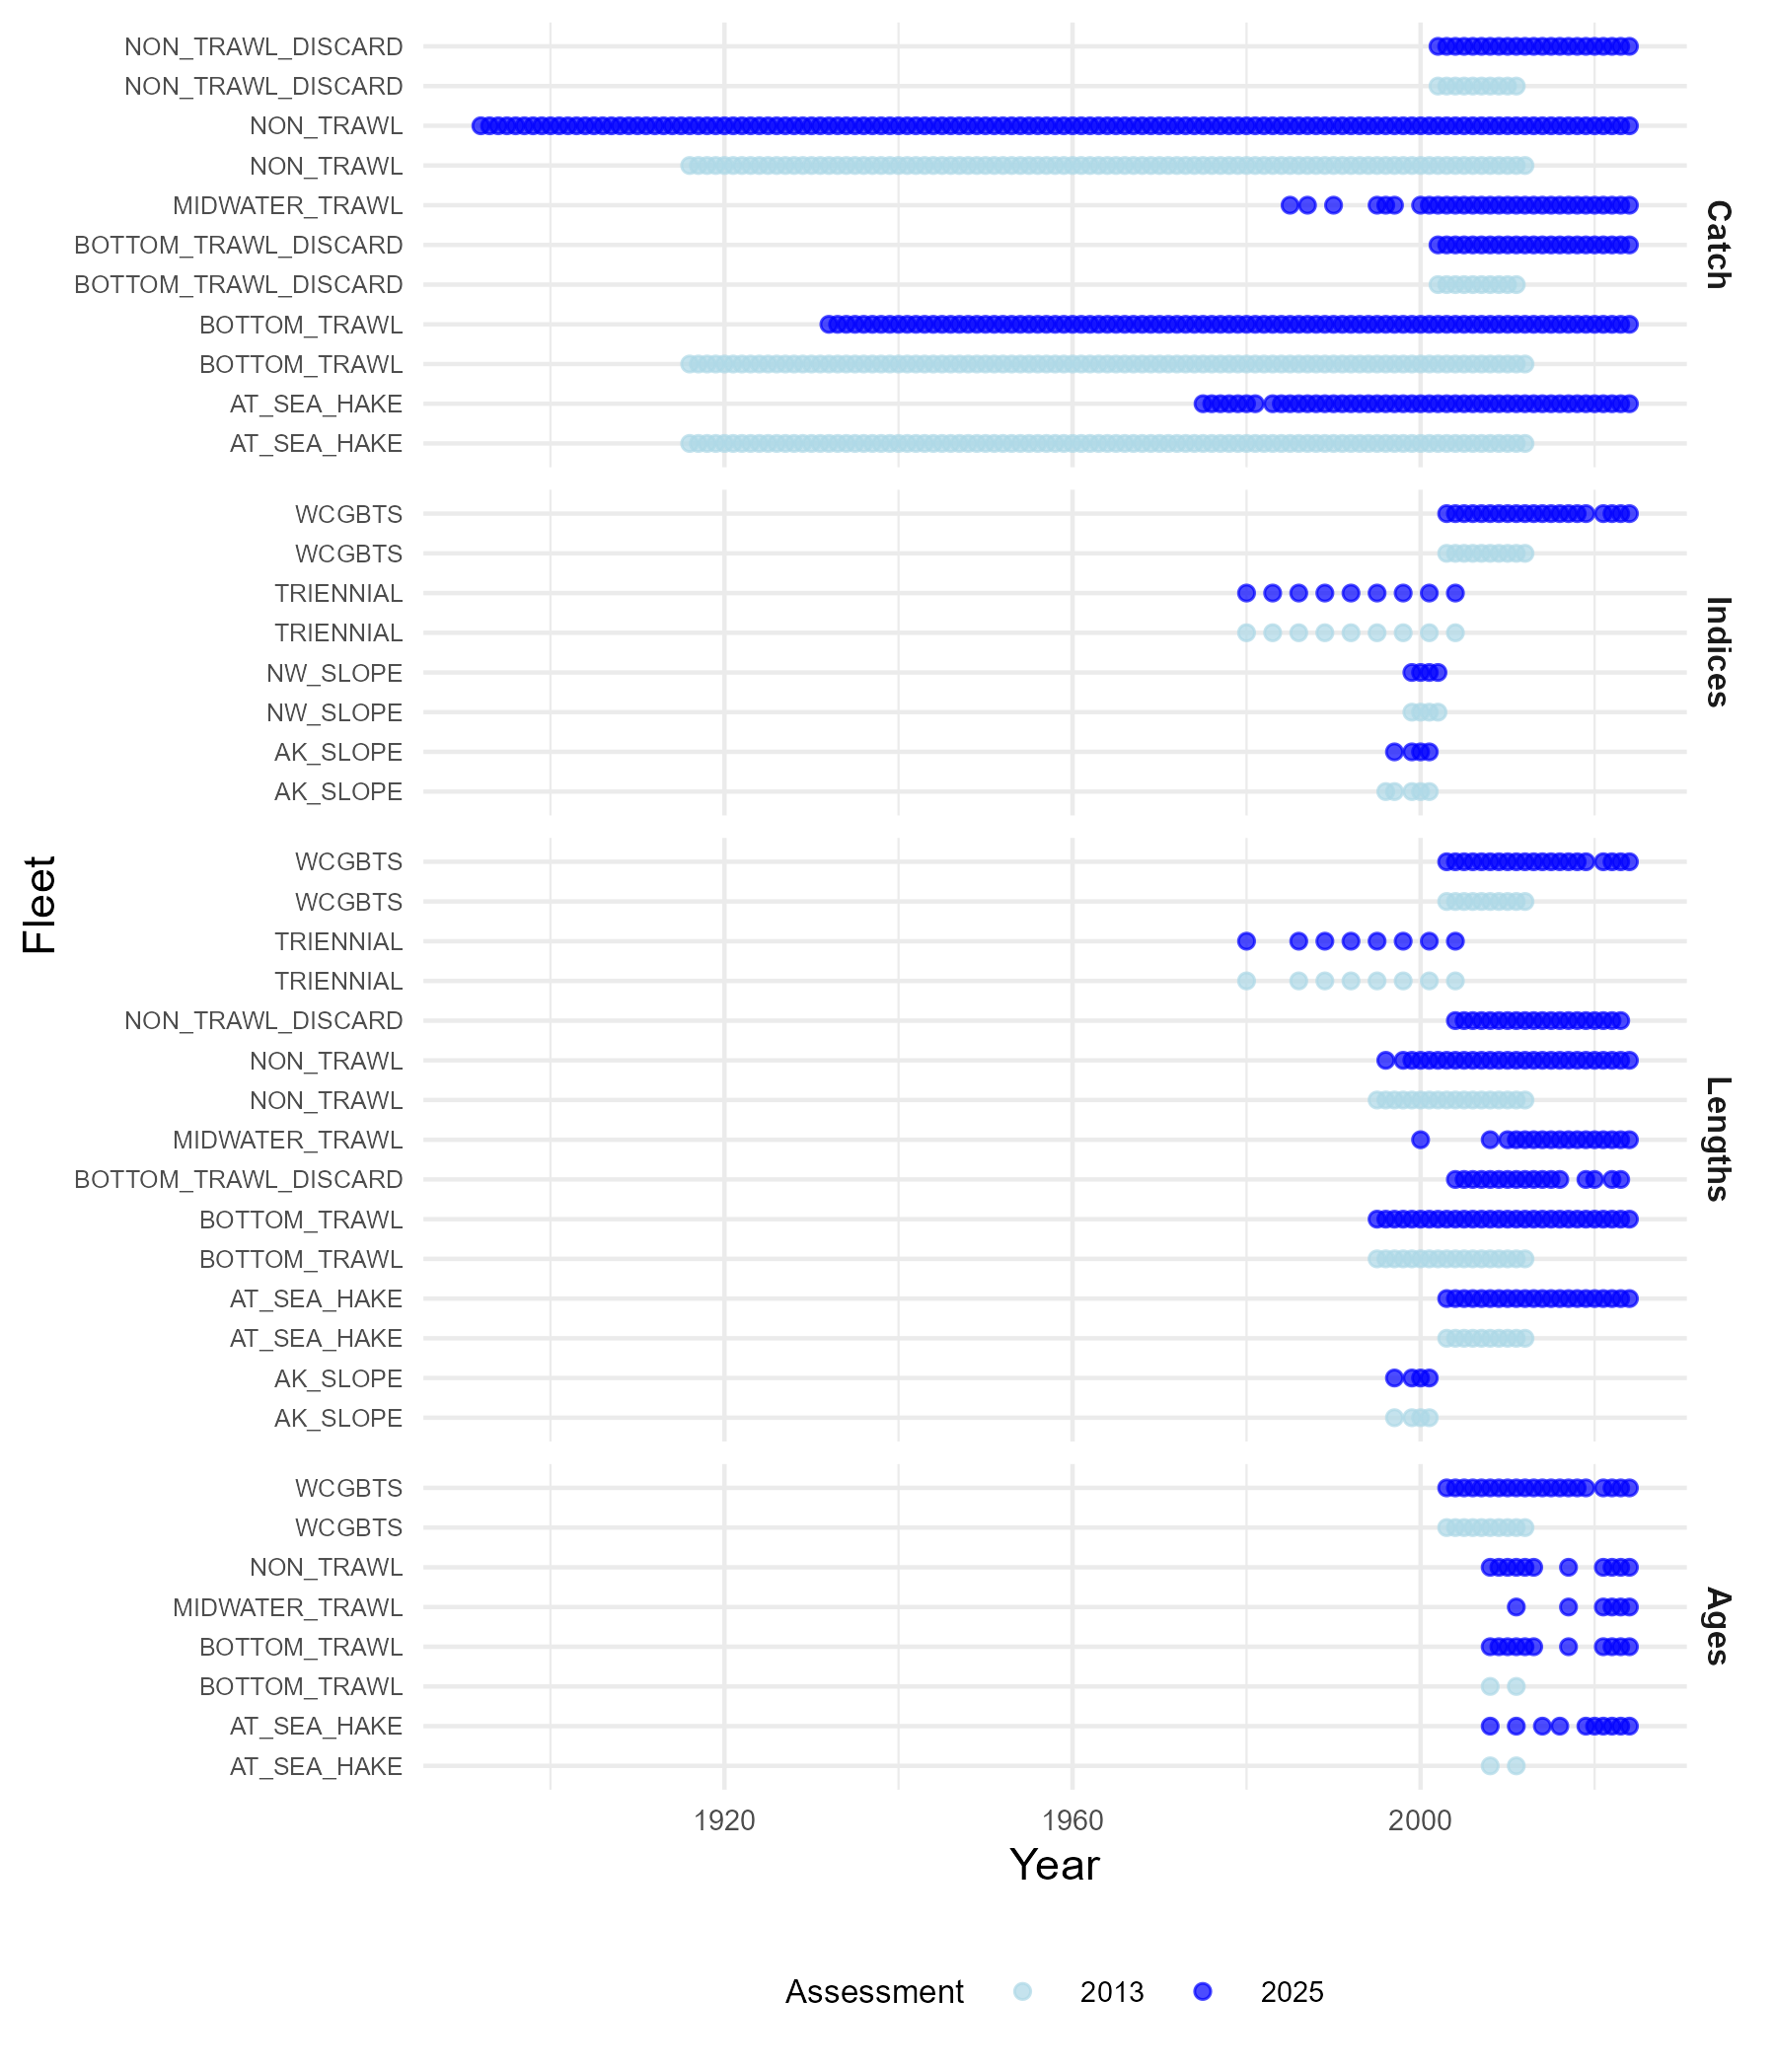
\includegraphics{plots_4_doc/data_comparison_2013_2025.png}

}

\caption{\label{fig-data-changes}Comparison of time series of the data
sources used in the 2025 Rougheye/Blackspotted rockfishes stock
assessment (current model, dark blue points) and the 2013 benchmark
assessment (light blue points). Bubble sizes represent relative total
catch standardized by the maximum total catch, relative sample size of
length data standardized by the maximum sample size of length data, and
relative sample size of age data standardized by the maximum sample size
of age data.}

\end{figure}%

\subsection{Model Output}\label{model-output}

\begin{figure}[H]

\centering{

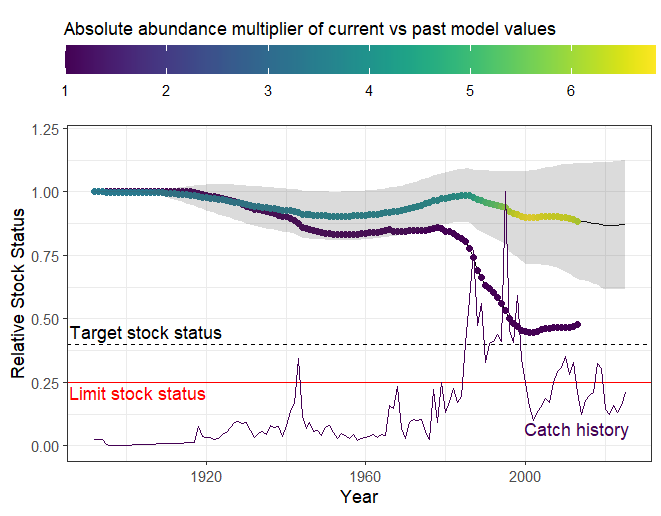
\includegraphics{plots_4_doc/Comp_2013_2025.png}

}

\caption{\label{fig-model-output-comp}Comparison of the 2025 (current
model) and the 2013 (last benchmark assessment) Rougheye/Blackspotted
rockfishes stock assessments using relative stock status (points) and
stock scale (color of the points). The gray envelope around the 2025
model are the 95\% uncertainty intervals for stock status. The catch
history (combined across fleets standardized to the largest value) is
given to compare the stock trajectory to the catch history. The OFL
sigma value from the stock assessment is 0.66, lower than the assumed
category 2 values of 1.0, but higher than what a category 1 stock would
be (0.5).}

\end{figure}%

\newpage

\subsection{Sources of Sensitivity}\label{sources-of-sensitivity}

\begingroup
\fontsize{9.0pt}{10.8pt}\selectfont

\begin{longtable}{lllll}

\caption{\label{tbl-uncertainty_summary_viz}Summary of uncertainty
sources and how they influence stock scale and relative status in the
Rougheye/Blackspotted rockfishes reference model.}

\tabularnewline

\toprule
Source & Source Option & Change & Scale & Status \\ 
\midrule\addlinespace[2.5pt]
Nautral mortlality &  & Increase & Up & Up \\ 
Bottom Trawl Selectivity &  &  &  &  \\ 
 & Logistic &  & Down & Down \\ 
 & Dome-shaped &  & Up & Up \\ 
Ageing Error &  & Less bias and imprecision & Down & Same \\ 
Data weighting &  &  &  &  \\ 
 & Lengths & Higher weight & Down & Down \\ 
 & Ages & Higher weight & Up & Up \\ 
 & WCGBTS Index & Removed & Down & Down \\ 
Recruitment estimation &  & Estimate fewer years & Up & Up \\ 
\bottomrule

\end{longtable}

\endgroup

\newpage{}

\section*{Executive Summary}\label{executive-summary}
\addcontentsline{toc}{section}{Executive Summary}

\subsection*{Stock}\label{stock}
\addcontentsline{toc}{subsection}{Stock}

This assessment reports the status of the Rougheye (\emph{Sebastes
aleutianus}) and Blackspotted (\emph{Sebastes melanostictus}) rockfishes
that reside in the waters off California, Oregon, and Washington from
the U.S.-Canadian border in the north to the U.S.-Mexico border in the
south.

These two species are difficult to differentiate visually in the catch,
thus they are commonly reported and treated as one management complex of
Rougheye/Blackspotted rockfishes (RE/BS). Despite recent advances in
genetic identification of Rougheye Rockfish and Blackspotted Rockfish,
there is still little ability to reliably separate historical fishery
data in order to differentiate these two species into two stocks.
Therefore, this assessment maintains a species complex approach, though
given Rougheye Rockfish tend to be encountered more often than
Blackspotted Rockfish off the U.S. West Coast, this may be considered
more of a Rougheye than Blackspotted Rockfish stock assessment. While we
treat these species as one stock complex, we recognize and are mindful
of the above species distinctions as we conduct our analyses.

\subsection*{Catches}\label{catches}
\addcontentsline{toc}{subsection}{Catches}

RE/BS are not targeted by a specific fishery, but are desirable and
marketable, thus are typically retained when caught.

The historical reconstruction of landings for RE/BS suggests that
non-trawl (largely hook-and-line gear) fisheries have caught RE/BS since
the end of the 19th century. The bottom trawl fishery developed in the
1930s and 1940s, and trawl landings for RE/BS first peaked in the 1960s
and 1970s, when the foreign trawl fleet was targeting Pacific Ocean
perch. The declaration of the Exclusive Economic Zone (established in
1977) resulted in the buildup of a domestic fleet and landings increased
rapidly into the late 1980s and early 1990s (generally \textgreater{}
300 mt with a peak of 745mt in 1995). Subsequently, landings declined in
the late 1990s, with catches under 250 metric tons in the last two
decades. The contribution of mid-water trawl catches gradually grew over
the past 15 years, and now they represent the majority of the trawl
removals.

Since RE/BS are marketable, discarding has been low historically.
However, management restrictions (e.g., trip limits) resulted in
increased discarding. Trawl rationalization was introduced in 2011, and
since then very little discarding of RE/BS has occurred.

RE/BS also has long been bycaught in the fishery for the coastal
population of Pacific Hake, which is almost exclusively conducted with
mid-water trawl.

Time series of landings are shown Figure~\ref{fig-es-landings}, with
recent landings detailed in Table~\ref{tbl-es-catches}.

\begingroup
\fontsize{7.5pt}{9.0pt}\selectfont

\begin{longtable}{ccccccccc}

\caption{\label{tbl-es-catches}Recent landings by fleet, total landings
summed across fleets, and the total dead catch including discards.}

\tabularnewline

\toprule
Year & Trawl & Trawl 
 discard & Non-trawl & Non-trawl 
 discard & Midwater 
 trawl & At-sea-hake & Total Landings & Total Dead \\ 
\midrule\addlinespace[2.5pt]
2015 & 30.67 & 0.01 & 46.56 & 13.79 & 19.26 & 21.80 & 132.09 & 132.09 \\ 
2016 & 30.79 & 0.11 & 60.27 & 12.61 & 15.53 & 29.63 & 148.95 & 148.95 \\ 
2017 & 21.93 & 0.00 & 59.03 & 34.42 & 2.48 & 38.15 & 156.02 & 156.02 \\ 
2018 & 16.49 & 0.00 & 46.67 & 14.55 & 2.58 & 161.24 & 241.52 & 241.52 \\ 
2019 & 22.06 & 0.04 & 38.75 & 31.13 & 9.25 & 125.37 & 226.59 & 226.59 \\ 
2020 & 9.86 & 0.03 & 24.35 & 1.03 & 28.92 & 41.88 & 106.07 & 106.07 \\ 
2021 & 10.33 & 0.01 & 21.06 & 2.36 & 21.39 & 37.62 & 92.76 & 92.76 \\ 
2022 & 11.54 & 0.02 & 19.06 & 2.72 & 18.63 & 65.46 & 117.43 & 117.43 \\ 
2023 & 13.29 & 0.48 & 18.67 & 0.48 & 26.22 & 38.50 & 97.63 & 97.63 \\ 
2024 & 9.97 & 0.12 & 9.90 & 0.48 & 69.15 & 29.32 & 118.94 & 118.94 \\ 
\bottomrule

\end{longtable}

\endgroup

\begin{figure}[H]

\centering{

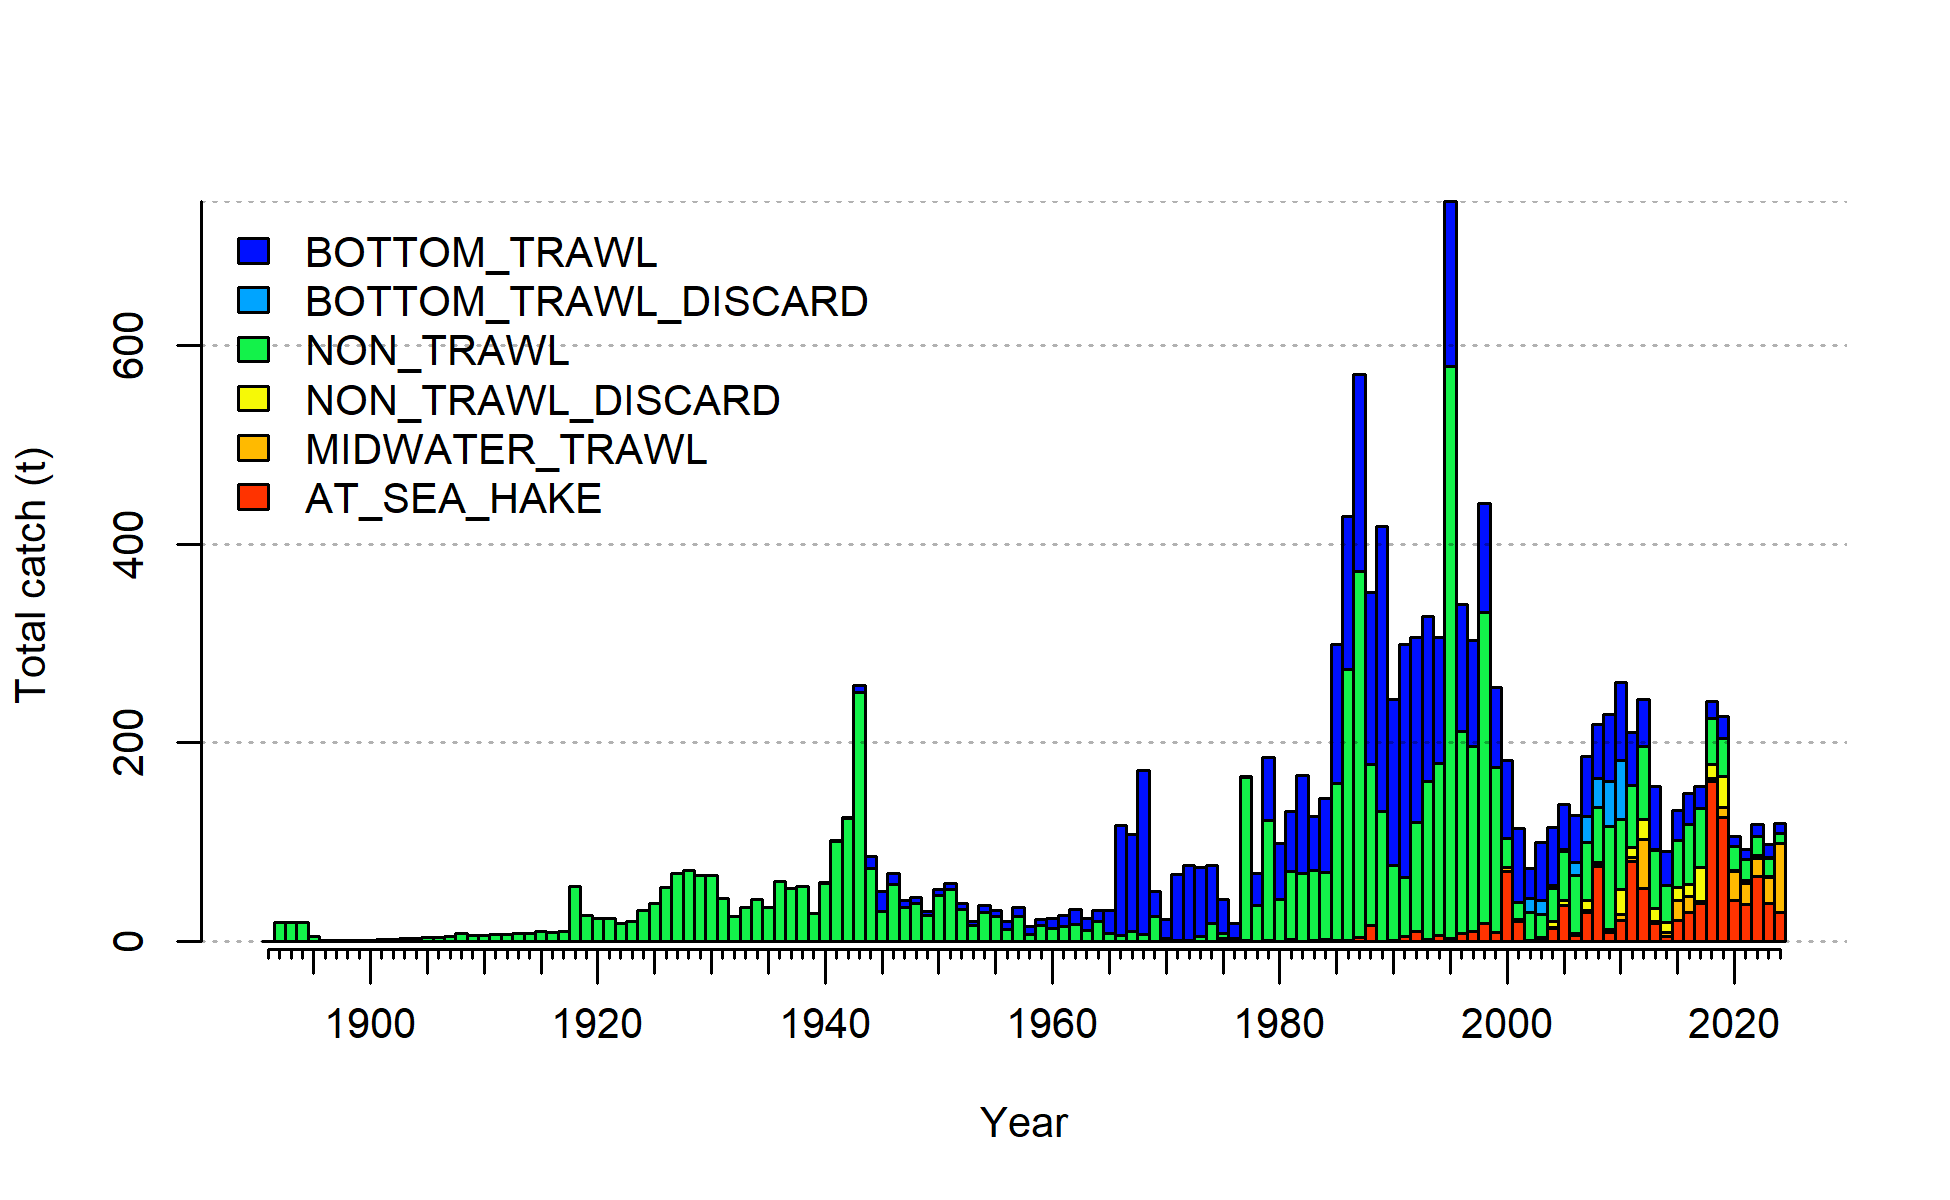
\includegraphics{ref_model/plots/catch2_landings_stacked.png}

}

\caption{\label{fig-es-landings}Landings in metric tons (mt) by year for
each fleet.}

\end{figure}%

\subsection*{Data and Assessments}\label{data-and-assessments}
\addcontentsline{toc}{subsection}{Data and Assessments}

The only previous RE/BS benchmark stock assessment for the U.S. West
Coast area was in 2013 (\citeproc{ref-hicks_status_2013}{Hicks et al.
2013}). It was conducted with the Stock Synthesis statistical
catch-at-age modelling framework (\citeproc{ref-MethotWetzel2013}{Methot
and Wetzel 2013}).

This 2025 assessment also uses Stock Synthesis, version 3.30.23.2. The
modeling period begins in 1892, and the stock prior to that is assumed
to be in an unfished equilibrium condition.

RE/BS fishery-dependent data in this assessment are divided among six
fleets, treating discard catches separately from the retained fisheries.
Following the 2013 assessment, it maintains the at-sea hake fishery as
its own fleet, and adds a mid-water fishery that has emerged in the last
decade. This stock assessment adds 10+ years of additional length data,
and several more years of age data (included as conditioned on length
data). The same four surveys (the West Coast Groundfish Bottom Trawl
Survey (WCGBTS), AFSC/NWFSC Triennial Shelf Survey, AFSC Slope Survey,
and NWFSC Slope Survey) as used in the last stock assessment are used
here, with the WCGBTS data extended to 2024. The index standardization
of all survey data uses the newer approach of applying spatiotemporal
generalized linear mixed models.

This is a sex-specific model. Females and males have separate growth
curves and sex-specific weight-at-length parameters. Growth is assumed
to follow the von Bertalanffy growth model, and the assessment
explicitly estimates all parameters describing somatic growth. The
natural mortality for females is estimated in the assessment and natural
mortality for males is fixed a the lowest value supported by the
likelihood profile, and is consistent with values associated with a
longevity of 150 years. Externally estimated life history parameters,
including those defining the length-weight relationship, female
fecundity and maturity schedule were revised for this assessment to
incorporate new information. Recruitment dynamics are assumed to follow
the Beverton-Holt stock-recruit function, and recruitment deviations are
estimated. Stock-recruitment steepness is fixed at the value generated
from a meta-analytical study on steepness in \emph{Sebastes} species
routinely used in West Coast groundfish assessments. The base model
estimates parameters for length-based selectivity, and estimated
selectivity curves are a mix of dome-shaped (for bottom trawl gears) and
logistic (for mid-water trawl).

\subsection*{Stock Output and Dynamics}\label{stock-output-and-dynamics}
\addcontentsline{toc}{subsection}{Stock Output and Dynamics}

The model estimates that the stock complex currently is in a healthy
state, well above management target (Figure~\ref{fig-es-sb},
Figure~\ref{fig-es-depl}). Approximate confidence intervals based on the
asymptotic variance estimates show that the uncertainty in the estimated
spawning output is high. Estimates of spawning output (in trillions of
eggs) in the most recent decade are shown in Table~\ref{tbl-es-sb}.

The fraction unfished shows a slight decline between the 1940s and the
1960s, and also a gradual decline since the early-1980s, which
correspond to the catch history.

\newpage

\begingroup
\fontsize{9.0pt}{10.8pt}\selectfont

\begin{longtable}{>{\centering\arraybackslash}p{\dimexpr 56.25pt -2\tabcolsep-1.5\arrayrulewidth}>{\centering\arraybackslash}p{\dimexpr 56.25pt -2\tabcolsep-1.5\arrayrulewidth}>{\centering\arraybackslash}p{\dimexpr 56.25pt -2\tabcolsep-1.5\arrayrulewidth}>{\centering\arraybackslash}p{\dimexpr 56.25pt -2\tabcolsep-1.5\arrayrulewidth}>{\centering\arraybackslash}p{\dimexpr 56.25pt -2\tabcolsep-1.5\arrayrulewidth}>{\centering\arraybackslash}p{\dimexpr 56.25pt -2\tabcolsep-1.5\arrayrulewidth}>{\centering\arraybackslash}p{\dimexpr 56.25pt -2\tabcolsep-1.5\arrayrulewidth}}

\caption{\label{tbl-es-sb}Estimated recent trend in spawning output and
the fraction unfished and the 95 percent confidence intervals.}

\tabularnewline

\toprule
Year & Spawning output (trillions of eggs) & Lower Interval (mt) & Upper Interval (mt) & Fraction Unfished & Lower Interval & Upper Interval \\ 
\midrule\addlinespace[2.5pt]
2015 & 4.912 & <0.001 & 12.096 & 0.881 & 0.650 & 1.113 \\ 
2016 & 4.900 & <0.001 & 12.085 & 0.879 & 0.645 & 1.113 \\ 
2017 & 4.886 & <0.001 & 12.071 & 0.877 & 0.640 & 1.113 \\ 
2018 & 4.871 & <0.001 & 12.056 & 0.874 & 0.635 & 1.114 \\ 
2019 & 4.846 & <0.001 & 12.031 & 0.870 & 0.625 & 1.114 \\ 
2020 & 4.825 & <0.001 & 12.013 & 0.866 & 0.617 & 1.115 \\ 
2021 & 4.823 & <0.001 & 12.016 & 0.865 & 0.615 & 1.116 \\ 
2022 & 4.827 & <0.001 & 12.029 & 0.866 & 0.615 & 1.117 \\ 
2023 & 4.832 & <0.001 & 12.050 & 0.867 & 0.614 & 1.120 \\ 
2024 & 4.845 & <0.001 & 12.083 & 0.869 & 0.615 & 1.123 \\ 
2025 & 4.860 & <0.001 & 12.124 & 0.872 & 0.617 & 1.127 \\ 
\bottomrule

\end{longtable}

\endgroup

\begin{figure}[H]

\centering{


\includegraphics{ref_model/plots/ts7_Spawning_output_with_95_intervals.png}

}

\caption{\label{fig-es-sb}Estimated time series of spawning output
(trillions of eggs) for the base model.}

\end{figure}%

\begin{figure}[H]

\centering{


\includegraphics{ref_model/plots/ts9_Relative_spawning_output_intervals.png}

}

\caption{\label{fig-es-depl}Estimated time series of fraction of
unfished spawning output for the base model.}

\end{figure}%

\subsection*{Recruitment}\label{recruitment}
\addcontentsline{toc}{subsection}{Recruitment}

Recruitment dynamics (Table~\ref{tbl-es-recr},
Figure~\ref{fig-es-recruits}) are assumed to follow the Beverton-Holt
stock-recruit function and the steepness parameter was fixed at the
value of 0.72, which is the mean of the steepness prior probability
distribution, derived from a meta-analysis of rockfish stocks. The level
of virgin recruitment (\(lnR_0\)) is estimated to inform the magnitude
of the initial stock size. Annual recruitment is treated as stochastic.
``Main'' recruitment deviations were estimated for modeled years between
1892 and 2023, with the forecast recruitment period starting in 2024
(Figure~\ref{fig-es-recdevs}).

\clearpage

\begingroup
\fontsize{9.0pt}{10.8pt}\selectfont

\begin{longtable}{>{\centering\arraybackslash}p{\dimexpr 56.25pt -2\tabcolsep-1.5\arrayrulewidth}>{\centering\arraybackslash}p{\dimexpr 56.25pt -2\tabcolsep-1.5\arrayrulewidth}>{\centering\arraybackslash}p{\dimexpr 56.25pt -2\tabcolsep-1.5\arrayrulewidth}>{\centering\arraybackslash}p{\dimexpr 56.25pt -2\tabcolsep-1.5\arrayrulewidth}>{\centering\arraybackslash}p{\dimexpr 56.25pt -2\tabcolsep-1.5\arrayrulewidth}>{\centering\arraybackslash}p{\dimexpr 56.25pt -2\tabcolsep-1.5\arrayrulewidth}>{\centering\arraybackslash}p{\dimexpr 56.25pt -2\tabcolsep-1.5\arrayrulewidth}}

\caption{\label{tbl-es-recr}Estimated recent trend in recruitment
(1,000s) and recruitment deviations and the 95 percent confidence
intervals.}

\tabularnewline

\toprule
Year & Recruitment (1,000s) & Lower Interval (1,000s) & Upper Interval (1,000s) & Recruitment Deviations & Lower Interval & Upper Interval \\ 
\midrule\addlinespace[2.5pt]
2015 & 652 & 173 & 2,459 & -0.445 & -1.271 & 0.382 \\ 
2016 & 861 & 228 & 3,253 & -0.172 & -1.012 & 0.668 \\ 
2017 & 2,147 & 585 & 7,885 & 0.737 & -0.010 & 1.484 \\ 
2018 & 1,326 & 354 & 4,972 & 0.250 & -0.565 & 1.066 \\ 
2019 & 1,184 & 317 & 4,415 & 0.132 & -0.678 & 0.943 \\ 
2020 & 837 & 221 & 3,170 & -0.220 & -1.083 & 0.643 \\ 
2021 & 913 & 236 & 3,529 & -0.138 & -1.050 & 0.773 \\ 
2022 & 1,006 & 254 & 3,979 & -0.046 & -1.008 & 0.916 \\ 
2023 & 1,056 & 266 & 4,195 & -0.003 & -0.982 & 0.975 \\ 
2024 & 1,064 & 268 & 4,230 & 0.000 & -0.980 & 0.980 \\ 
\bottomrule

\end{longtable}

\endgroup

\begin{figure}[H]

\centering{


\includegraphics{ref_model/plots/ts11_Age-0_recruits_(1000s)_with_95_asymptotic_intervals.png}

}

\caption{\label{fig-es-recruits}Estimated time series of age-0 recruits
for the base model.}

\end{figure}%

\begin{figure}[H]

\centering{


\includegraphics{ref_model/plots/recdevs2_withbars.png}

}

\caption{\label{fig-es-recdevs}Estimated time series of recruitment
deviations for the base model.}

\end{figure}%

\subsection*{Exploitation Status}\label{exploitation-status}
\addcontentsline{toc}{subsection}{Exploitation Status}

Two measures of exploitation are fishing intensity and exploitation
rate. Fishing intensity is defined here as 1 - \(SPR\), where \(SPR\)
(Spawning Potential Ratio) is the equilibrium spawning output at a given
combination of F and selectivity relative to spawning output at unfished
equilibrium. Using the units of 1-\(SPR\) means that more intense
fishing is associated with a higher value. The value of 1-\(SPR\) in the
absence of fishing is 0 and the maximum is 1.0 if all spawning fish are
killed before spawning. The Pacific Fishery Management Council (PFMC)
has chosen an \(SPR\) target of 0.5 for RE/BS, so harvest which leads to
\(SPR\) below 0.5 (or fishing intensity (1-\(SPR\)) greater than 0.5)
would be overfishing. Exploitation rate is defined as the catch relative
to age 26+ biomass, which refers to the age at functional maturity. This
metric is included to aid interpretation of stock status, but it is not
used as a basis for management.

Exploitation rates were below the management target of a fishing
intensity that leads to a \(SPR\) of 0.5 throughout most of the time
series except for 1995, when the catch peaked at 744 metric tons
(Table~\ref{tbl-es-spr}, Figure~\ref{fig-es-spr}).

\begingroup
\fontsize{9.0pt}{10.8pt}\selectfont

\begin{longtable}{>{\centering\arraybackslash}p{\dimexpr 60.00pt -2\tabcolsep-1.5\arrayrulewidth}>{\centering\arraybackslash}p{\dimexpr 60.00pt -2\tabcolsep-1.5\arrayrulewidth}>{\centering\arraybackslash}p{\dimexpr 60.00pt -2\tabcolsep-1.5\arrayrulewidth}>{\centering\arraybackslash}p{\dimexpr 60.00pt -2\tabcolsep-1.5\arrayrulewidth}>{\centering\arraybackslash}p{\dimexpr 60.00pt -2\tabcolsep-1.5\arrayrulewidth}>{\centering\arraybackslash}p{\dimexpr 60.00pt -2\tabcolsep-1.5\arrayrulewidth}>{\centering\arraybackslash}p{\dimexpr 60.00pt -2\tabcolsep-1.5\arrayrulewidth}}

\caption{\label{tbl-es-spr}Estimated recent trend in fishing intensity
1-SPR, where SPR is the spawning potential ratio, and the exploitation
rate, along with the 95 percent confidence intervals for both
quantities.}

\tabularnewline

\toprule
Year & 1-SPR & Lower Interval (SPR) & Upper Interval (SPR) & Exploitation Rate & Lower Interval (Rate) & Upper Interval (Rate) \\ 
\midrule\addlinespace[2.5pt]
2015 & 0.115 & <0.001 & 0.267 & 0.005 & <0.001 & 0.011 \\ 
2016 & 0.129 & <0.001 & 0.297 & 0.005 & <0.001 & 0.013 \\ 
2017 & 0.134 & <0.001 & 0.309 & 0.005 & <0.001 & 0.013 \\ 
2018 & 0.190 & <0.001 & 0.425 & 0.008 & <0.001 & 0.021 \\ 
2019 & 0.182 & <0.001 & 0.410 & 0.008 & <0.001 & 0.019 \\ 
2020 & 0.091 & <0.001 & 0.215 & 0.004 & <0.001 & 0.009 \\ 
2021 & 0.080 & <0.001 & 0.191 & 0.003 & <0.001 & 0.008 \\ 
2022 & 0.099 & <0.001 & 0.234 & 0.004 & <0.001 & 0.010 \\ 
2023 & 0.084 & <0.001 & 0.200 & 0.004 & <0.001 & 0.009 \\ 
2024 & 0.100 & <0.001 & 0.234 & 0.004 & <0.001 & 0.011 \\ 
\bottomrule

\end{longtable}

\endgroup

\begin{figure}[H]

\centering{

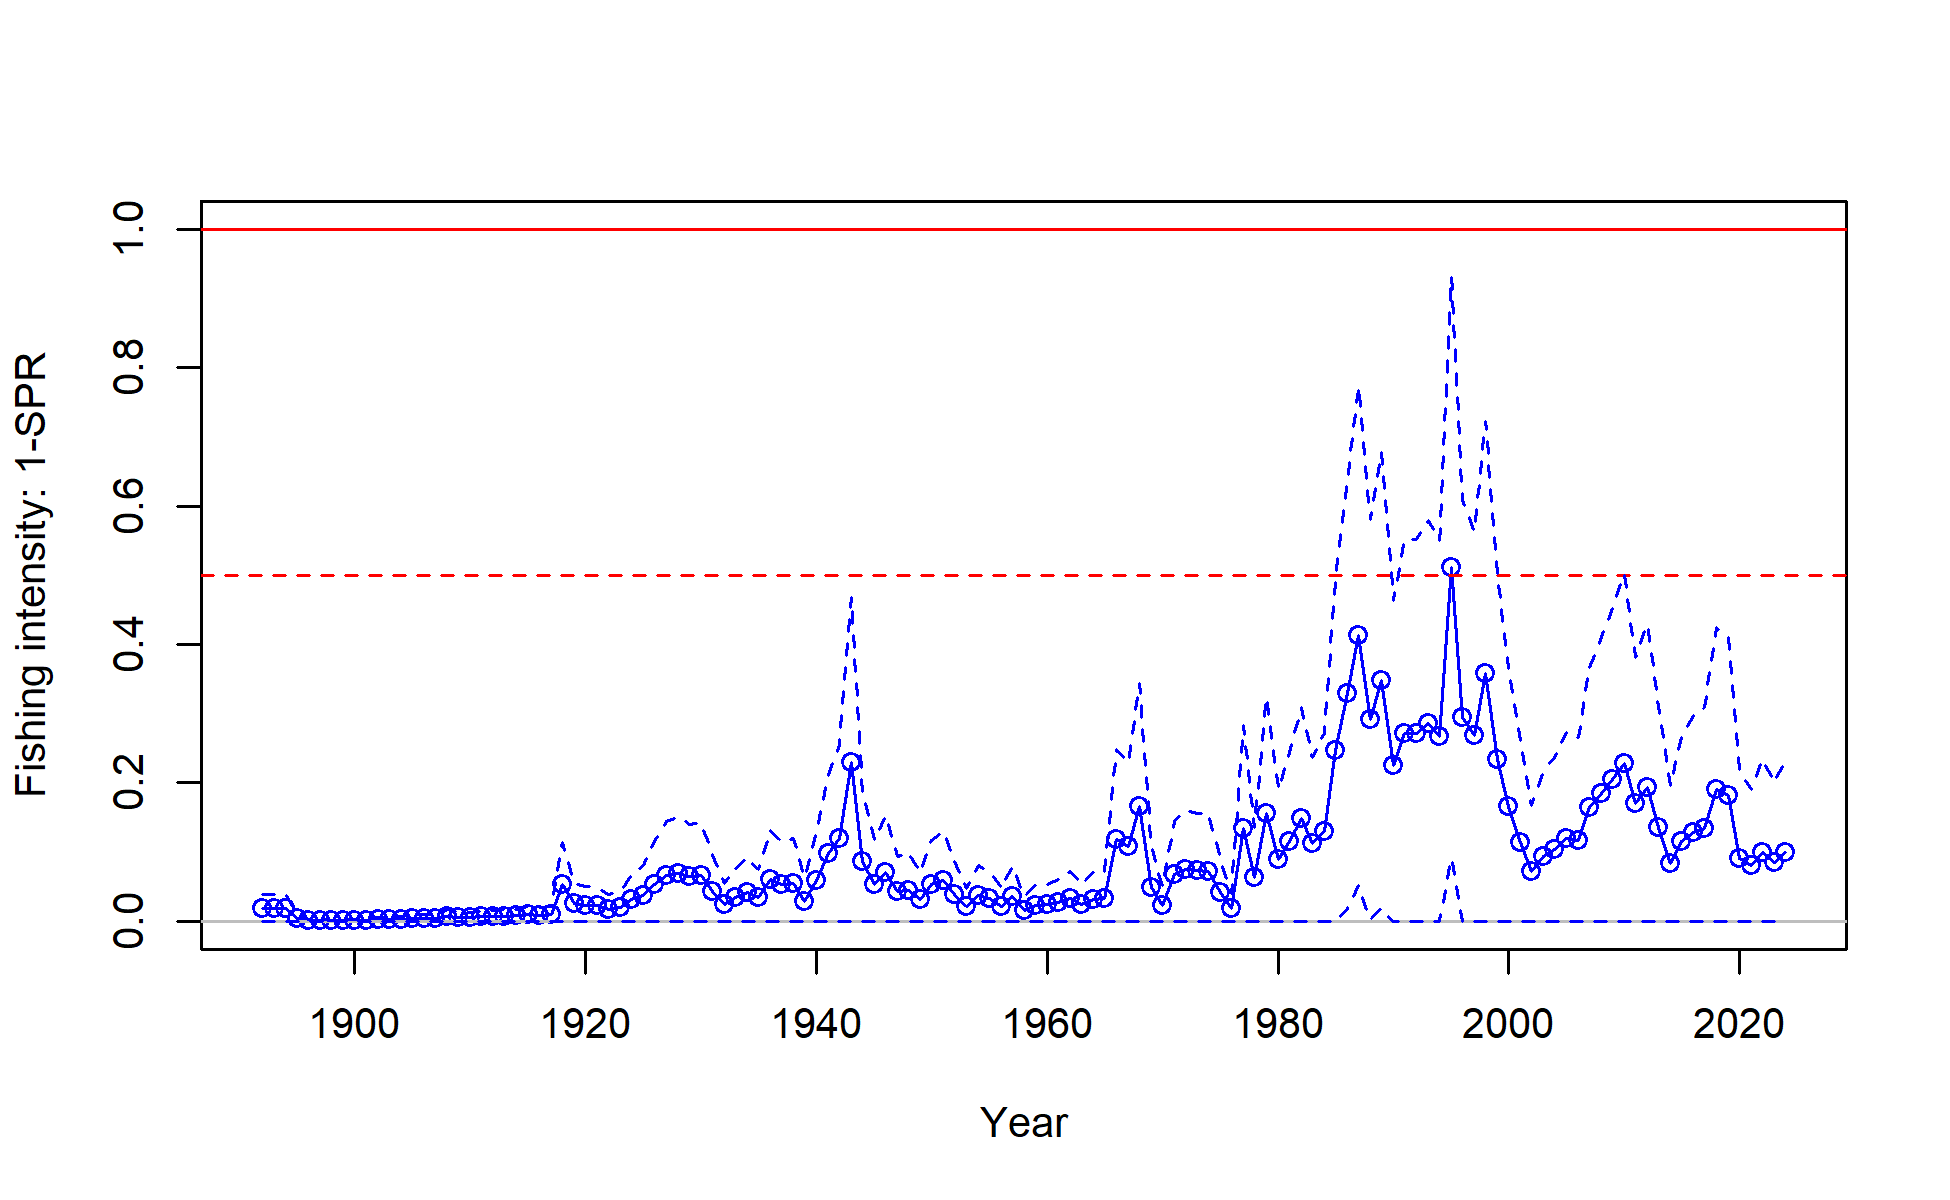
\includegraphics{ref_model/plots/SPR3_ratiointerval.png}

}

\caption{\label{fig-es-spr}Estimated time series of the fishing
intensity (1 - \(SPR\)), where \(SPR\) is the spawning potential ratio,
with approximate 95\% asymptotic intervals. The horizontal line at 0.5
corresponds to \(SPR\) = 0.5, the management reference point. The
horizontal line at 1.0 corresponds to \(SPR\) = 0 (all spawning fish
removed from the population).}

\end{figure}%

\subsection*{Ecosysystem
Considerations}\label{ecosysystem-considerations}
\addcontentsline{toc}{subsection}{Ecosysystem Considerations}

Rockfishes are an important component of the California Current
ecosystem along the U.S. West Coast, with its many dozens of species
filling various niches in both soft and hard bottom habitats from the
nearshore to the continental slope. RE/BS are one of the larger species
of rockfishes and occupy shelf areas when they are young and move into
deeper slope waters with age. As they age, they tend to become more
solitary, but may form aggregations during the spawning season. Due to a
paucity of life-history data for RE/BS, most ecosystem considerations
are implied from the understanding of rockfishes in general.

Recruitment is one mechanism by which the ecosystem may directly impact
the population dynamics of RE/BS. The specific pathways through which
environmental conditions exert influence on RE/BS dynamics are unclear.
However, changes in water temperature and currents, distribution of prey
and predators, and the amount and timing of upwelling are all possible
linkages. Changes in the environment may also result in changes in
age-at-maturity, fecundity, growth, and survival which can affect how
the status of the stock and its susceptibility to fishing are
determined. Unfortunately, there are no data for RE/BS that provide
insights into these effects.

\subsection*{Reference Points}\label{reference-points}
\addcontentsline{toc}{subsection}{Reference Points}

Reference points (Table~\ref{tbl-ref-points-es}) were calculated using
the estimated fishery selectivity and removals in the most recent year
of the model (2024). Reference points were based on the rockfish
\(\text{F}_{MSY\%}\) proxy (\(\text{SPR}_{50\%}\)), target relative
biomass (40\%), and estimated selectivity and catch for each fleet
(Table~\ref{tbl-ref-points-es}). The proxy MSY values of management
quantities are by definition more conservative compared to the estimated
MSY and MSY relative to 40\% of unfished spawning output because of the
assumed steepness value. Sustainable total yield, removals, using the
proxy \(\text{SPR}_{50\%}\) is 519.31 mt. The spawning output equivalent
to 40\% of the unfished spawning output (\(\text{SO}_{40\%}\))
calculated using the \(SPR\) target (\(\text{SPR}_{50\%}\)) was 2.48651
trillions of eggs.

The 2025 spawning output relative to unfished equilibrium spawning
output, based on the 2024 fishing year, is 87\%, above the management
target of 40\% of unfished spawning output (Figure~\ref{fig-es-depl}).
The fishing intensity, \(1-SPR\), was below to just slightly above
harvest rate limit (\(SPR_{50\%}\)) from the mid-1980s through the
1990s. Removals since 2000 have been below the point estimate of
potential long-term yields calculated using an \(\text{SPR}_{50\%}\)
reference point (Table~\ref{tbl-ts} and Figure~\ref{fig-es-spr}).

The relative biomass and the ratio of the estimated \(SPR\) to the
management target (\(\text{SPR}_{50\%}\)) across all model years are
shown in Figure~\ref{fig-es-kobe}. The stock status has not decreased
below the target relative biomass, and fishing intensity (except for in
1995) has been below the target fishing intensity based on
\(\text{SPR}_{50\%}\).

\begingroup
\fontsize{9.0pt}{10.8pt}\selectfont

\begin{longtable}{lrlr}

\caption{\label{tbl-ref-points-es}Summary of reference points and
management quantities, including estimates of the 95 percent confidence
intervals. SO is spawning output (in trillions of eggs), SPR is the
spawning potential ratio, and MSY is maximum sustainable yield.}

\tabularnewline

\toprule
Reference Point & Estimate & Lower Interval & Upper Interval \\ 
\midrule\addlinespace[2.5pt]
Unfished Spawning output & 5.573 & <1 & 12.328 \\ 
Unfished Age 26+ Biomass (mt) & 33,189 & <1 & 73,425 \\ 
Unfished Recruitment (R0) & 1,077 & <1 & 2,371 \\ 
2025 Spawning output & 4.860 & <1 & 12.124 \\ 
2025 Fraction Unfished & 0.872 & 0.617 & 1.127 \\ 
Reference Points Based SO40\% & — & — & — \\ 
Proxy Spawning output SO40\% & 2.229 & <1 & 4.931 \\ 
SPR Resulting in SO40\% & 0.458 & 0.458 & 0.458 \\ 
Exploitation Rate Resulting in SO40\% & 0.048 & 0.045 & 0.051 \\ 
Yield with SPR Based On SO40\% (mt) & 545 & <1 & 1,200 \\ 
Reference Points Based on SPR Proxy for MSY & — & — & — \\ 
Proxy Spawning output (SPR50) & 2.487 & <1 & 5.500 \\ 
SPR50 & 0.500 & — & — \\ 
Exploitation Rate Corresponding to SPR50 & 0.040 & 0.038 & 0.042 \\ 
Yield with SPR50 at SO SPR (mt) & 519 & <1 & 1,142 \\ 
Reference Points Based on Estimated MSY Values & — & — & — \\ 
Spawning output at MSY (SO MSY) & 1.477 & <1 & 3.270 \\ 
SPR MSY & 0.337 & 0.334 & 0.339 \\ 
Exploitation Rate Corresponding to SPR MSY & 0.085 & 0.079 & 0.090 \\ 
MSY (mt) & 585 & <1 & 1,285 \\ 
\bottomrule

\end{longtable}

\endgroup

\begin{figure}[H]

\centering{

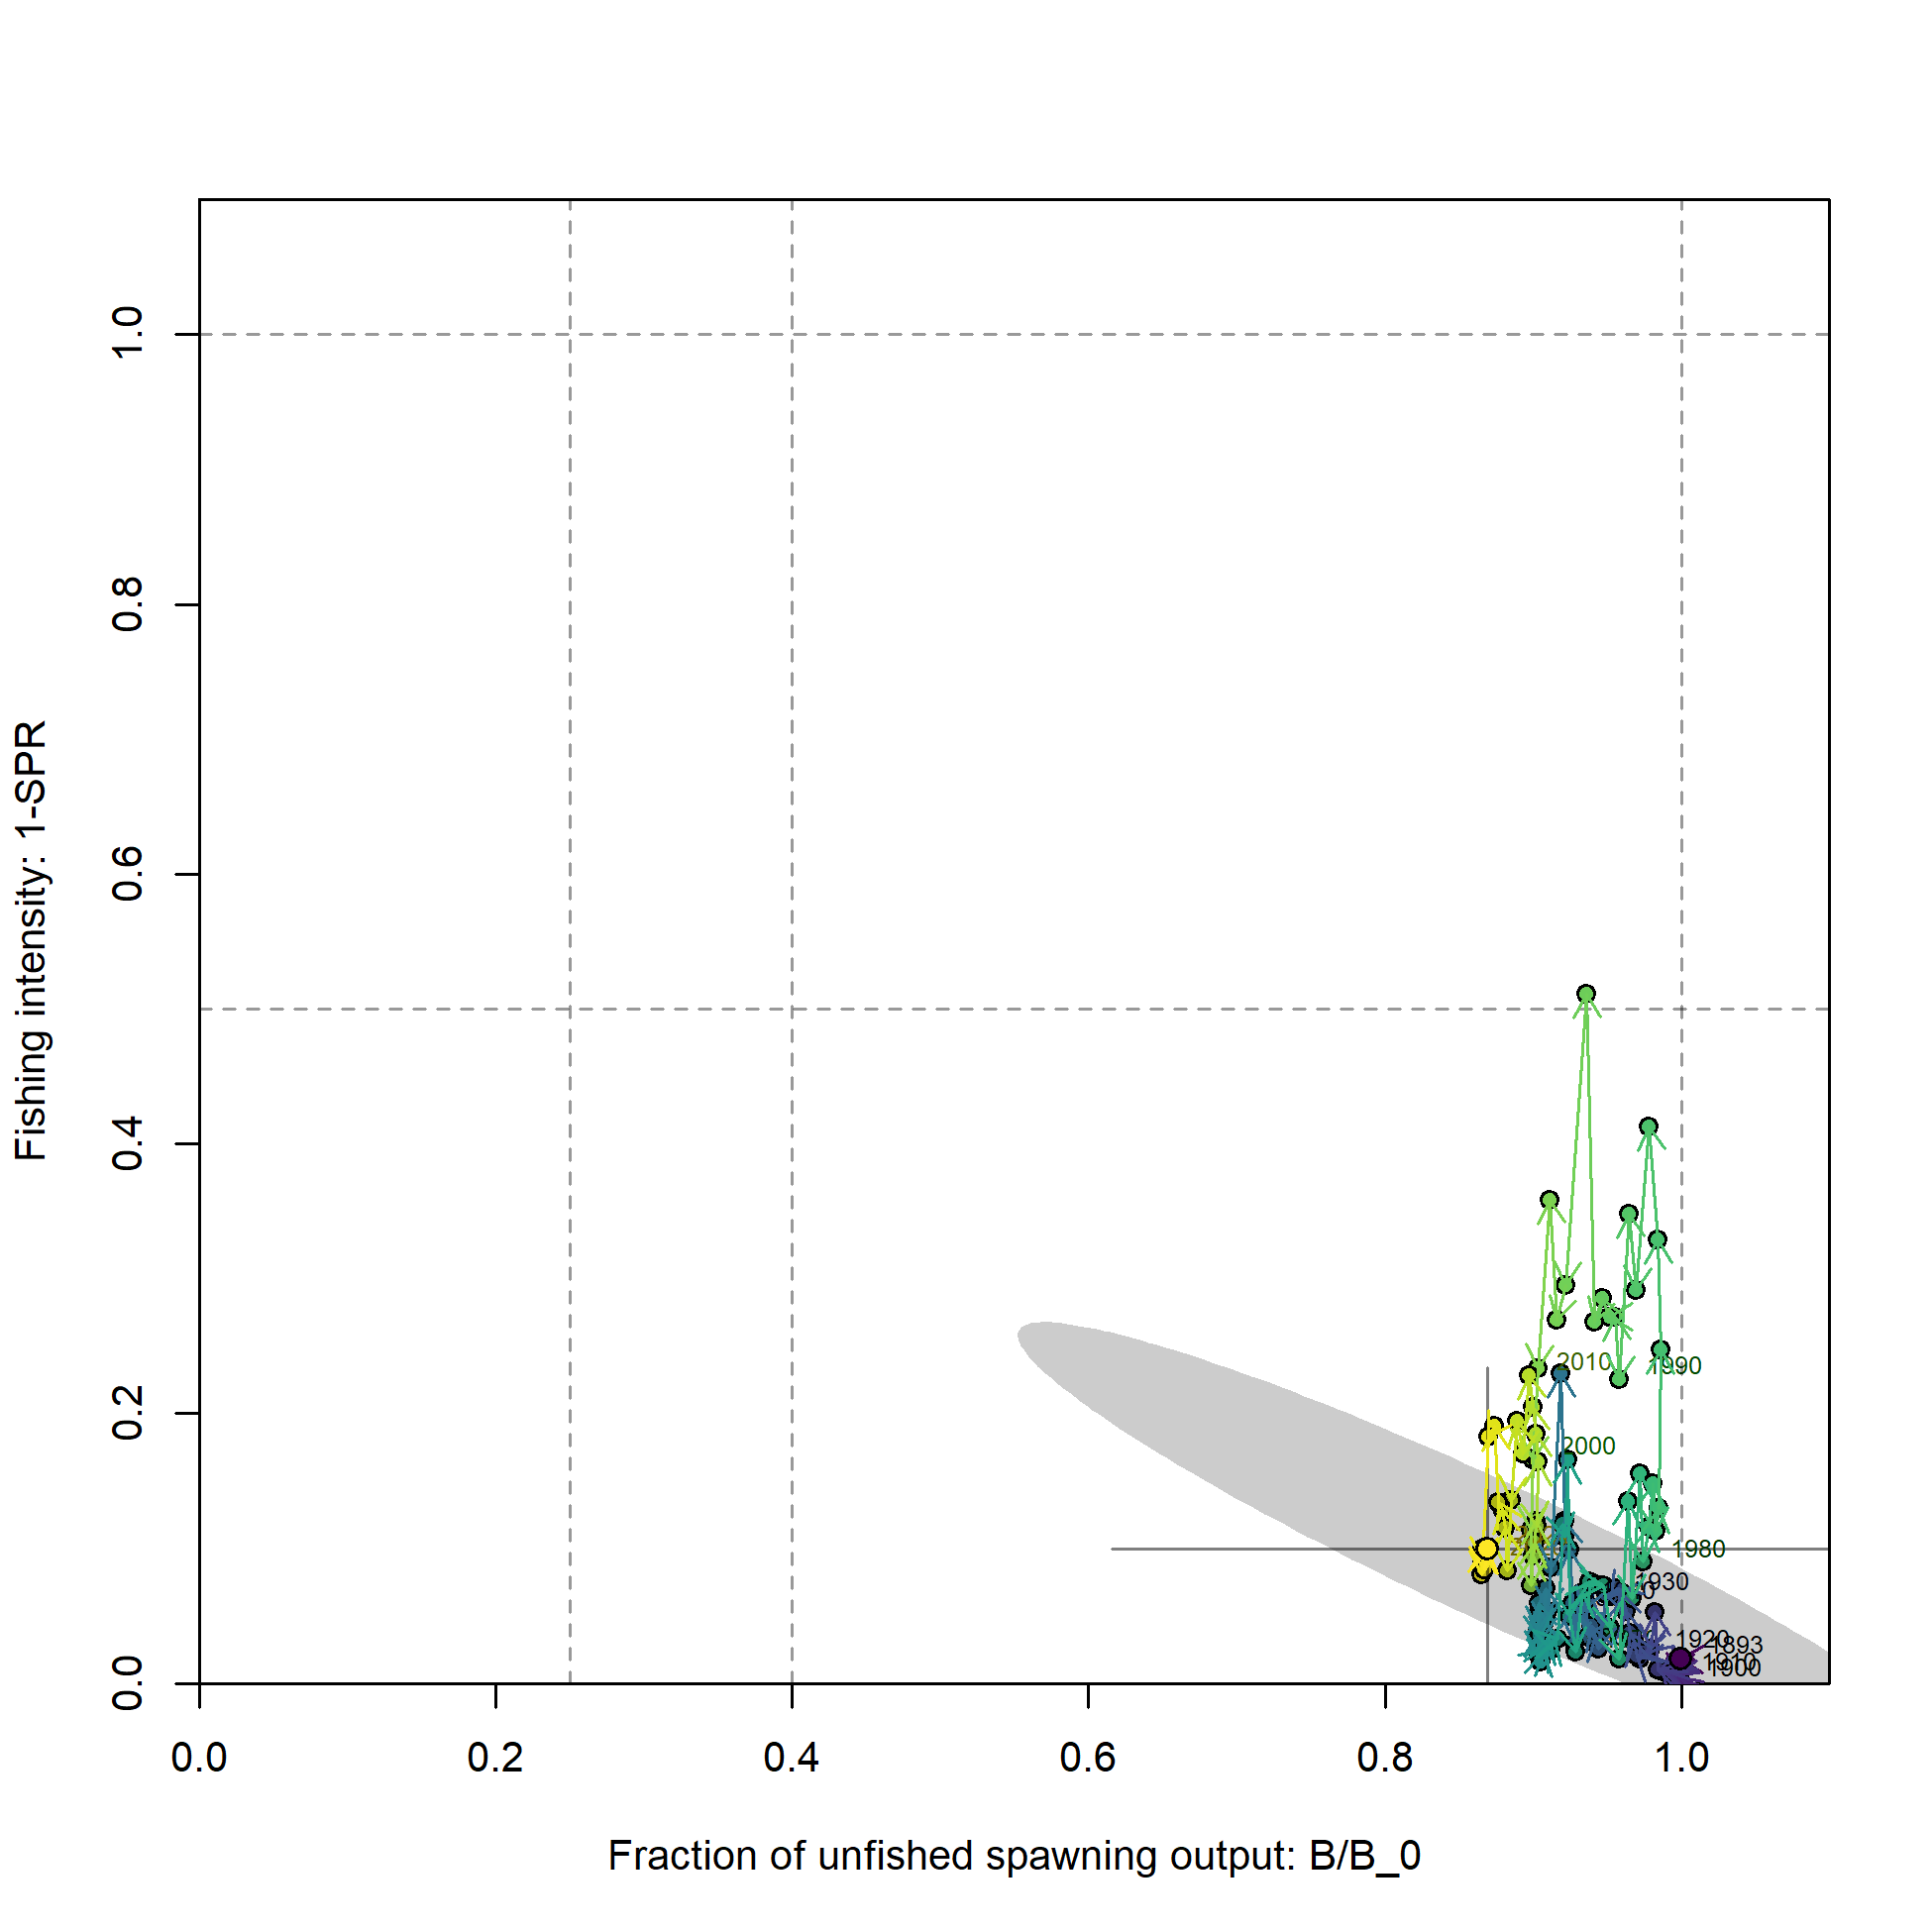
\includegraphics{ref_model/plots/SPR4_phase.png}

}

\caption{\label{fig-es-kobe}Phase plot of fishing intensity versus
fraction unfished. Each point represents the biomass ratio at the start
of the year and the relative fishing intensity in that same year. Cooler
colors (purple) represent early years and warmer colors (yellow)
represent recent years. Lines through the final point show 95\%
intervals based on the asymptotic uncertainty for each dimension. The
shaded ellipse is a 95\% region which accounts for the estimated
correlation between the two quantities.}

\end{figure}%

\subsection*{Management Performance}\label{management-performance}
\addcontentsline{toc}{subsection}{Management Performance}

The last ten years of total dead catches for RE/BS against the component
overfishing limits (OFLs), the acceptable biological catches (ABCs), the
annual catch limits (ACLs) are shown in Table~\ref{tbl-es-management}.
In the last ten years, total dead catches of RE/BS have been below the
component OFLs for most years, with exception of 2018 and 2019. However,
exceeding component OFLs does not indicate overfishing, since the stock
is managed as part of a complex.

\begingroup
\fontsize{9.0pt}{10.8pt}\selectfont

\begin{longtable}{rrrrr}

\caption{\label{tbl-es-management}Recent trend in the overfishing limits
(OFL), the acceptable biological catches (ABCs), the annual catch limits
(ACLs), and the total dead catch (landings + discards) all in metric
tons (mt). Specifications are combined across north and south of 40'10.}

\tabularnewline

\toprule
Year & OFL (mt) & ABC (mt) & ACL (mt) & Catch (mt) \\ 
\midrule\addlinespace[2.5pt]
2015 & 206 & 188 & 188 & 132 \\ 
2016 & 211 & 193 & 193 & 149 \\ 
2017 & 215 & 196 & 196 & 156 \\ 
2018 & 219 & 200 & 200 & 242 \\ 
2019 & 222 & 203 & 203 & 227 \\ 
2020 & 224 & 204 & 204 & 106 \\ 
2021 & 237 & 196 & 196 & 93 \\ 
2022 & 238 & 195 & 195 & 117 \\ 
2023 & 238 & 193 & 193 & 98 \\ 
2024 & 238 & 195 & 195 & 119 \\ 
\bottomrule

\end{longtable}

\endgroup

\subsection*{Unresolved Problems and Major
Uncertainties}\label{unresolved-problems-and-major-uncertainties}
\addcontentsline{toc}{subsection}{Unresolved Problems and Major
Uncertainties}

The absolute size of RE/BS populations are highly uncertain. Through
extensive explorations, we found that stock scale is sensitive to
assumptions about the shape of the selectivity curves, especially for
the bottom trawl. In the previous assessment, selectivity for all fleets
(except for the Triennial Survey) was assumed to be asymptotic. In this
assessment, we provided flexibility for the bottom trawl and non-trawl
fleets and bottom trawl surveys to estimate dome-shaped selectivity
curves. Changes in selectivity assumptions enabled substantially
improved fits to length and age composition data in fisheries and
surveys, but also resulted in a substantial increase of stock scale.

Stock scale was also sensitive to assumptions about natural mortality.
RE/BS is one of the longest lived species of rockfish on the West Coast,
with maximum ages of 169 years in this assessment. An individual in
Alaska was reported to be 205 years (Munk
(\citeproc{ref-munkMaximumAgesGroundfishes2001}{2001})), the oldest ever
aged rockfish. It is therefore likely that natural mortality for RE/BS
is lower than for other rockfish species. With length and age data
available only for years after 1994, there is limited ability to monitor
the long-term changes of aging cohorts. Therefore, estimates of natural
mortality are uncertain. This assessment attempts to capture uncertainty
in this parameter and integrate it into the derived biomass estimates by
estimating natural mortality for females, while fixing the male natural
mortality at the lowest value still supported by the likelihood profile.

\subsection*{Scientific Uncertainty}\label{scientific-uncertainty}
\addcontentsline{toc}{subsection}{Scientific Uncertainty}

The model estimated uncertainty (\(\sigma\)) around the 2025 spawning
output is 0.68. The uncertainty around the OFL is 0.66. These values
underestimate the overall uncertainty as they do not incorporate the
model structural uncertainty and do not account for any time-varying
dynamics other than recruitment. The estimated uncertainty values are
lower than the Category 2 default of 1, so all projections will use the
Category 2 default.

\subsection*{Decision Table and Harvest
Projections}\label{decision-table-and-harvest-projections}
\addcontentsline{toc}{subsection}{Decision Table and Harvest
Projections}

The primary axis of uncertainty used in the decision table is natural
mortality. Male natural mortality in the assessment model is fixed at
\(M = 0.036\), the value informed by likelihood profile and based on a
meta-analytical prior that corresponds to the maximum age of 150 years.
The natural mortality value for the low state of nature is \(M = 0.032\)
and for high state of nature is \(M = 0.039\).

For the low state of nature the value was selected based in
meta-analytic prior to correspond to maximum age of 169 years, which is
oldest fish observed in the dataset used in the assessment. For the high
state of nature, the value was selected based on the likelihood profile
to be higher than in the base model, but still reasonable given the
species biology; it corresponds to maximum age of 138 years based on
meta-analytic prior.

Twelve-year forecasts were calculated for each state of nature. The 2025
and 2026 catches are fixed at values provided by GMT. For the rest of
the years, we used base model forecast catches calculated using the
default harvest control rule P\(^*\) = 0.45, and Category 2 default
\(\sigma = 1\). The alternative states of nature (Low, Base, and High)
are provided in the columns of Table~\ref{tbl-es-decision-1}, with
Spawning Output and Fraction of unfished provided for each state. The
sigma value from the decision table for the low state of nature model is
0.83.

Projections of the overfishing limit, acceptable biological catch, and
annual catch limit, all based on a \(P^*\) of 0.45 and a log-space
standard deviation of the overfishing limit (\(\sigma\)) of 1 are
included in Table~\ref{tbl-es-projections}. Assumed catches for 2025 and
2026 for this projection were provided by the PFMC Groundfish Management
Team, and catches from 2027 onward assume full attainment of the
acceptable biological catch.

\begin{table}[H]

\caption{\label{tbl-es-decision-1}Decision table with 12-year
projections. The alternative states of nature (`Low', `Base', and `High'
as discussed in the text) are provided in the columns, with Spawning
Output (`Spawn', in trillions of eggs) and Fraction of unfished spawning
output (`Frac') provided for each state.}

\centering{

\centering\centering
\fontsize{9}{11}\selectfont
\begin{tabular}[t]{>{}llr>{\raggedleft\arraybackslash}p{3.5em}>{\raggedleft\arraybackslash}p{3.5em}>{\raggedleft\arraybackslash}p{3.5em}>{\raggedleft\arraybackslash}p{3.5em}>{\raggedleft\arraybackslash}p{3.5em}>{\raggedleft\arraybackslash}p{3.5em}}
\toprule
Mgmt & Year & Catch & Low Spawn & Low Frac & Base Spawn & Base Frac & High Spawn & High Frac\\
\midrule
\textbf{A} & 2025 & 155.1 & 1.98 & 0.733 & 4.86 & 0.872 & 13.08 & 0.933\\
\textbf{} & 2026 & 186.7 & 1.99 & 0.734 & 4.87 & 0.875 & 13.13 & 0.936\\
\textbf{} & 2027 & 843.9 & 1.99 & 0.735 & 4.89 & 0.877 & 13.18 & 0.939\\
\textbf{} & 2028 & 825.7 & 1.91 & 0.705 & 4.82 & 0.865 & 13.15 & 0.937\\
\textbf{} & 2029 & 808.8 & 1.83 & 0.677 & 4.76 & 0.854 & 13.12 & 0.936\\
\textbf{} & 2030 & 792.2 & 1.76 & 0.650 & 4.70 & 0.843 & 13.10 & 0.934\\
\textbf{} & 2031 & 776.0 & 1.69 & 0.624 & 4.64 & 0.833 & 13.09 & 0.933\\
\textbf{} & 2032 & 760.0 & 1.62 & 0.598 & 4.59 & 0.823 & 13.07 & 0.932\\
\textbf{} & 2033 & 745.2 & 1.55 & 0.574 & 4.53 & 0.813 & 13.06 & 0.931\\
\textbf{} & 2034 & 729.5 & 1.49 & 0.550 & 4.48 & 0.804 & 13.04 & 0.930\\
\textbf{} & 2035 & 713.9 & 1.42 & 0.527 & 4.43 & 0.795 & 13.02 & 0.928\\
\textbf{} & 2036 & 699.4 & 1.36 & 0.504 & 4.38 & 0.786 & 13.00 & 0.927\\
\bottomrule
\end{tabular}

}

\end{table}%

\clearpage

\begin{landscape}
\begingroup
\fontsize{9.0pt}{10.8pt}\selectfont

\begin{longtable}{>{\centering\arraybackslash}p{\dimexpr 56.25pt -2\tabcolsep-1.5\arrayrulewidth}>{\centering\arraybackslash}p{\dimexpr 56.25pt -2\tabcolsep-1.5\arrayrulewidth}>{\centering\arraybackslash}p{\dimexpr 56.25pt -2\tabcolsep-1.5\arrayrulewidth}>{\centering\arraybackslash}p{\dimexpr 56.25pt -2\tabcolsep-1.5\arrayrulewidth}>{\centering\arraybackslash}p{\dimexpr 56.25pt -2\tabcolsep-1.5\arrayrulewidth}>{\centering\arraybackslash}p{\dimexpr 56.25pt -2\tabcolsep-1.5\arrayrulewidth}>{\centering\arraybackslash}p{\dimexpr 56.25pt -2\tabcolsep-1.5\arrayrulewidth}>{\centering\arraybackslash}p{\dimexpr 56.25pt -2\tabcolsep-1.5\arrayrulewidth}>{\centering\arraybackslash}p{\dimexpr 56.25pt -2\tabcolsep-1.5\arrayrulewidth}>{\centering\arraybackslash}p{\dimexpr 56.25pt -2\tabcolsep-1.5\arrayrulewidth}}

\caption{\label{tbl-es-projections}Potential OFLs (mt), ABCs (mt), ACLs
(mt), the buffer between the OFL and ABC, estimated spawning output, and
fraction unfished with adopted OFLs and ACLs and assumed catch for the
first two years of the projection period.}

\tabularnewline

\toprule
Year & Adopted OFL (mt) & Adopted ACL (mt) & Assumed Catch (mt) & OFL (mt) & Buffer & ABC (mt) & ACL (mt) & Spawning output (trillions of eggs) & Fraction Unfished \\ 
\midrule\addlinespace[2.5pt]
2025 & 238 & 189 & 155 & — & — & — & — & 4.860 & 0.872 \\ 
2026 & 237 & 187 & 187 & — & — & — & — & 4.875 & 0.875 \\ 
2027 & — & — & — & 966 & 0.874 & 844 & 844 & 4.888 & 0.877 \\ 
2028 & — & — & — & 955 & 0.865 & 826 & 826 & 4.821 & 0.865 \\ 
2029 & — & — & — & 944 & 0.857 & 809 & 809 & 4.758 & 0.854 \\ 
2030 & — & — & — & 933 & 0.849 & 792 & 792 & 4.698 & 0.843 \\ 
2031 & — & — & — & 923 & 0.841 & 776 & 776 & 4.641 & 0.833 \\ 
2032 & — & — & — & 912 & 0.833 & 760 & 760 & 4.586 & 0.823 \\ 
2033 & — & — & — & 902 & 0.826 & 745 & 745 & 4.533 & 0.813 \\ 
2034 & — & — & — & 892 & 0.818 & 729 & 729 & 4.480 & 0.804 \\ 
2035 & — & — & — & 881 & 0.810 & 714 & 714 & 4.429 & 0.795 \\ 
2036 & — & — & — & 871 & 0.803 & 699 & 699 & 4.378 & 0.786 \\ 
\bottomrule

\end{longtable}

\endgroup

\end{landscape}

\subsection*{Research and Data Needs}\label{research-and-data-needs}
\addcontentsline{toc}{subsection}{Research and Data Needs}

There are many areas of research that would benefit the understanding
and assessment of RE/BS. Below, we identify several of them that we
consider particularly important.

\begin{itemize}
\item
  Continued research on distinguishing biology of Rougheye and
  Blackspotted rockfishes: This assessment reports the status of RE/BS
  as a pooled complex because it is extremely difficult to separate the
  catches of each species even in recent data, and attempting to do so
  would greatly increase the uncertainty in the predictions. Because
  little is known about the respective biology and catch histories of
  the two species, it is unclear whether managing them as a complex may
  place one species at disproportionate risk of overfishing relative to
  the other. New research presented in this document shows potential
  differences in maturity between the species. Additional research that
  will provide insight into the distribution, life history, biological
  characteristics, and catch and discard profiles of the two species is
  recommended. Such an endeavor would likely require the efforts of
  at-sea observers in all fleets, biologists aboard fishery-independent
  surveys, and port samplers along the entire West Coast, requiring
  broad, inter-agency collaboration.
\item
  Understanding of coastwide stock structure, connectivity, and
  distribution: This is a stock assessment for RE/BS off of the west
  coast of the U.S. and does not consider data from British Columbia or
  Alaska. Further investigating and comparing the data and predictions
  from British Columbia and Alaska to determine if there are
  similarities with the U.S. West Coast observations would help to
  define the connectivity between Rougheye/Blackspotted Rockfishes north
  of the U.S.-Canada border.
\item
  Natural mortality: Uncertainty in natural mortality translates into
  uncertain estimates of status and sustainable fishing levels for
  RE/BS. The assessment model was able to estimate female natural
  mortality, consistent with maximum age based meta-analytical prior,
  but male natural mortality was fixed in the model. Given what seems to
  be a current population with a deep age structure, the collection of
  additional age data and further research of the life-history of RE/BS
  may improve our understanding of RE/BS natural mortality.
\item
  Increasing the number of ageing samples. This assessment increased the
  number of available aged samples by the thousands, but many more are
  needed to resolve the age structure, as well as add to our
  understanding of how the age structure has and is changing over time.
  This will include the consideration of improving the ageing error of
  these species, with a consideration towards decreasing the number of
  ageing error matrices needed, or improving the imprecision of some of
  the current ageing error matrices. This would necessitate the
  re-reading of otoliths (in addition to reading new otoliths).
\item
  Developing and applying new age determination techniques, such as
  Fourier Transform Near-Infrared spectroscopy (FT-NIR): In recent
  years, progress has been made in using FT-NIR approach for fish age
  determination. At present, FT-NIR ages for RE/BS have low agreement
  with traditional age estimates, and further research is needed before
  they are incorporated into stock assessment. Given the longevity of
  these species, more age data is needed per year compared to other
  rockfishes in order to define the age structure. The longevity also
  makes ageing these species more difficult. More rapid ageing
  techniques may help achieve the numbers needed to track age structure
  changes.
\item
  Historical landings and discards, including investigation of fisheries
  selectivity: Substantial progress has been made in reconstructing
  historical landings of rockfishes on the U.S. West Coast, including
  those for RE/BS. This assessment highlighted the importance of
  understanding fishery selectivity assumptions associated with removals
  and how fishery selectivity changes throughout the years. Further
  understanding and discussion on likely selectivity forms over time
  would help reduce uncertainty in the estimated scale of the stock.
\item
  Otolith structure may prove to be a distinguishing feature to
  determine Rougheye from Blackspotted rockfishes
  (\citeproc{ref-harris_using_2019}{Harris et al. 2019}). We encourage
  more research into this, to assist achieving species-specific
  identification into the future, and potentially into the past.
\item
  Consider whether the International Pacific Halibut Commission survey
  may contribute biological samples and possibly an additional index to
  any future assessments.
\end{itemize}

\subsection*{Risk Table}\label{risk-table}
\addcontentsline{toc}{subsection}{Risk Table}

A risk table was constructed using the Category 1 stock rubric, but is
not included here given this stock assessment is considered Category 2.
The risk table can be found in the Appendix.

\newpage{}

\setlength{\parskip}{5mm plus1mm minus1mm}
\pagenumbering{arabic}
\setcounter{page}{1}
\setcounter{section}{0}
\renewcommand{\thefigure}{\arabic{figure}}
\setcounter{figure}{0}
\renewcommand{\thetable}{\arabic{table}}
\setcounter{table}{-1}

\section{Introduction}\label{introduction}

Rougheye (\emph{Sebastes aleutianus}) and Blackspotted (\emph{Sebastes
melanostictus}) rockfishes are two species that form one management
complex of Rougheye/Blackspotted rockfishes (RE/BS).

Rougheye Rockfish are a long-lived rockfish named after a series of 2-10
spines along the lower rim of their eyes. They have also been called
Blackthroat or Blacktip Rockfish
(\citeproc{ref-love_rockfishes_2002}{Love et al. 2002};
\citeproc{ref-love_certainly_2011}{Love 2011}). Blackspotted Rockfish
are distributed in similar locations as Rougheye Rockfish and it is very
difficult to visually distinguish the two species. These two species may
hybridize on occasion (\citeproc{ref-love_certainly_2011}{Love 2011}).

It has only been from recent genetic studies that these two separate
species have been identified
(\citeproc{ref-hawkins_genetic_2005}{Hawkins et al. 2005};
\citeproc{ref-gharrett_genetically_2006}{Gharrett et al. 2006}) and have
had phenotypic characteristics useful for distinguishing the species in
the field identified (\citeproc{ref-gharrett_genetically_2006}{Gharrett
et al. 2006}; \citeproc{ref-orr_species_2008}{Orr and Hawkins 2008}).
Before then, data were available for one species called Rougheye
Rockfish that included Rougheye Rockfish and Blackspotted Rockfish. Due
to the difficulty in distinguishing these two species and the lack of
historical separation of the species in all of the data, this assessment
combines any data for Blackspotted Rockfish with Rougheye Rockfish into
RE/BS and provides management advice for the two species combined. These
species are also closely related to Shortraker Rockfish (\emph{Sebastes
borealis}) and are sometimes difficult to distinguish from Shortraker
Rockfish without looking at the gill rakers.

\subsection{Stock Structure}\label{sec-stock_structure}

There are at least two questions to think about when considering stock
structure for RE/BS when doing a stock assessment.

\begin{itemize}
\tightlist
\item
  Since Rougheye and Blackspotted Rockfishes are two different species,
  can they be separated as two stocks and conduct separate assessments?
\end{itemize}

Rougheye Rockfish were first described in 1811 as \emph{Perca
variabilis} by German zoologist Peter Simon Pallas
(\citeproc{ref-jordan_fishes_1898}{Jordan and Evermann 1898}), and
assigned to various taxa at least 15 times since
(\citeproc{ref-love_rockfishes_2002}{Love et al. 2002}). Some
descriptions noted both light and dark color morphs, which, along with
possible confusion with several morphologically similar co-occurring
species (e.g., \emph{Sebastes borealis} and \emph{Sebastes
melanostomus}), have contributed to the persistent ambiguity in formal
descriptions of Rougheye Rockfish (\citeproc{ref-orr_species_2008}{Orr
and Hawkins 2008}). The first genetic studies conducted in the late
1960s and early 1970s (\citeproc{ref-tsuyuki_contribution_1968}{Tsuyuki
et al. 1968}; \citeproc{ref-tsuyuki_analyses_1970}{Tsuyuki and Westrheim
1970}) observed diversity suggestive of two genetic types within
specimens identified as Rougheye Rockfish. Allozyme studies conducted
over the next two decades (\citeproc{ref-seeb_biochemical_1986}{Seeb
1986}; \citeproc{ref-hawkins_genetic_1997}{Hawkins et al. 1997};
\citeproc{ref-hawkins_genetic_2005}{Hawkins et al. 2005}) provided
additional evidence suggesting two separate genetic types within
field-identified Rougheye Rockfish. Genetic variation between the two
types, supported by both nuclear and mitochondrial DNA, was determined
to be sufficiently conclusive to separate two species: ``Type I'' and
``Type II'' Rougheye Rockfish (\citeproc{ref-gharrett_two_2005}{Gharrett
et al. 2005}). Meristic and morphometric comparisons of the two species
suggested certain characters, such as gill raker counts and length,
snout length, anal base length, and pectoral fin base, were
significantly different, and in combination could reliably, though not
definitively, distinguish between the species
(\citeproc{ref-gharrett_genetically_2006}{Gharrett et al. 2006}). The
two separate species were formally re-described by Orr and Hawkins
(\citeproc{ref-orr_species_2008}{2008}) with the Type II group retaining
\emph{Sebastes aleutianus} and the common name Rougheye Rockfish.
Blackspotted Rockfish was proposed as the common name for the Type I
group along with the scientific name of \emph{Sebastes melanostictus},
re-establishing nomenclature from one of the species complex's earlier
descriptions (\citeproc{ref-matsubara_1934}{Matsubara 1934}).

These two species remain difficult to consistently differentiate
visually in the catch, thus are still commonly reported and treated as a
species complex. Otolith morphometrics (e.g., shape, size, weight) have
shown some promise in possibly identifying these species in Alaskan
waters (97.3\% Blackspotted and 86.2\% of Rougheye rockfishes were
accurately identified) and possibly using older otoliths to break out
historical information by species
(\citeproc{ref-harris_using_2019}{Harris et al. 2019}). Frey et al.~(in
prep.) provided insight into the ability of the Northwest Fisheries
Science Center West Coast Groundfish Bottom Trawl Survey biologists to
identify the two species, with 90\% of genetically identified Rougheye
Rockfish being correctly identified in the field. When
mis-identifications occurred, it was usually a Blackspotted rockfish
being mis-identified as a Rougheye Rockfish. There were few
mis-identifications when a fish was identified as a Blackspotted
rockfish. While this is promising for potential future species-specific
data coming from the survey, it does not alleviate the historical
problem of separating fishery data into the two species. Frey et al.~(in
prep.) therefore also considered whether ecological factors like depth
or latitude could help separate samples by species. They found that both
species occur within the range of this assessment's considered areas
(California to Washington), and heavily spatially overlap.
Interestingly, there seem to be relative hot spots for these species
where one species is more common than the other, and in general,
Rougheye Rockfish seems to be more common than Blackspotted Rockfish;
however, Blackspotted Rockfish may be the more common of the two in
parts of Alaska (\citeproc{ref-gharrett_two_2005}{Gharrett et al. 2005};
\citeproc{ref-hawkins_genetic_2005}{Hawkins et al. 2005};
\citeproc{ref-orr_species_2008}{Orr and Hawkins 2008}).

Despite recent advances in species identification of Rougheye Rockfish
and Blackspotted Rockfish as genetically distinct species, there is
little ability to separate current or historical fishery data reliably
in order to separate these two species into two stocks. Therefore, this
assessment maintains a species complex approach, though given absolute
presence off the U.S. West Coast, this may be considered more of a
Rougheye than a Blackspotted Rockfish stock assessment. We also note
that throughout the range of these stocks, all current assessments to
this point have maintained a species complex approach. While we treat
these species as one assessed stock complex, we recognize and are
mindful of the above species distinctions as we conduct our analyses.

\begin{itemize}
\tightlist
\item
  Both species range into Canada and Alaska -- are they one stock?
\end{itemize}

While genetics studies have focused mostly on identification of the two
species, little is known about the population structure of either
species. This assessment and the 2013 assessment
(\citeproc{ref-hicks_status_2013}{Hicks et al. 2013}) represent the most
southerly range of these species. Comparing the absolute abundance of
the 2013 assessment to the most current estimates of the Alaskan stocks,
the absolute number in this southerly range is much smaller than in the
Gulf of Alaska (GOA), but similar to the Bering Sea/Aleutian Island
(BSAI) stock (Figure~\ref{fig-SO_comp}). The two smaller stocks have
similar trends of decline and stabilization, whereas the higher biomass
GOA stock looks to have not dropped at all over the time period
considered (Figure~\ref{fig-RSS_comp}). In spite of uncertainty in the
stock structure, we assume here that the West Coast stocks of RE/BS are
distinct management units from those in Alaska.

\subsection{Distribution}\label{distribution}

RE/BS range from northern California up to and throughout Alaska and
into Japan (\citeproc{ref-gharrett_two_2005}{Gharrett et al. 2005};
\citeproc{ref-hawkins_genetic_2005}{Hawkins et al. 2005};
\citeproc{ref-orr_species_2008}{Orr and Hawkins 2008}). Both are
long-lived (\textgreater100 years), with Rougheye Rockfish having the
distinction of the oldest ever aged \emph{Sebastes} species at 205 years
old (\citeproc{ref-munkMaximumAgesGroundfishes2001}{Munk 2001}). They
both greatly overlap in latitude and depth (shallower than 100 m to at
least 439 m), and are generally considered slope rockfish, with an
ontogenetic shift from shallower to deeper, and adults commonly found at
360 m (around 200 fathoms). Rougheye seems to be proportionally more
abundant when survey samples are genetically identified, and
Blackspotted Rockfish tend to be found, on average, deeper than Rougheye
Rockfish (\citeproc{ref-hawkins_genetic_2005}{Hawkins et al. 2005};
\citeproc{ref-orr_species_2008}{Orr and Hawkins 2008}).

RE/BS are often associated with structure, such as hard, rocky bottoms
and steep habitats. They are rarely found on the deep flats. They can be
found alone or in aggregations (\citeproc{ref-love_rockfishes_2002}{Love
et al. 2002}), with aggregations often differentiated by age. Younger
fish may school and are often found in shallower waters on the shelf,
juveniles and sub-adults can be found together, and larger fish may form
larger aggregations during the autumn and winter.

This assessment treats the U.S. RE/BS resource from the Mexican border
to the Canadian border as a single coastwide stock
(Figure~\ref{fig-map}). The U.S.-Canadian border is the northern
boundary for the assessed stock, although the basis for this choice is
due to political and current management needs rather than the population
dynamics. The assessment excludes consideration of the Salish Sea. RE/BS
primarily occur in the the northern part of the assessed area
(Figure~\ref{fig-cpue-map}).

\subsection{Life History}\label{life-history}

Like all \emph{Sebastes} species, RE/BS give birth to live young.
Parturition has been documented between February and June with larvae
lengths at parturition are between 4.5-5.3 mm
(\citeproc{ref-love_rockfishes_2002}{Love et al. 2002}). Dick et al.
(\citeproc{ref-dick_meta-analysis_2017}{2017}) showed that rockfishes
exhibit a non-proportional relationship of fecundity to weight, with
larger individuals producing more eggs than expected only by weight.
Although neither Rougheye nor Blackspotted Rockfishes have a species- or
subfamily-specific estimate for this relationship, this stock assessment
uses the unobserved genus \emph{Sebastes} values to inform fecundity to
weight relationship for RE/BS.

A wide range of prey items make up the diet of RE/BS. Crangonid and
pandalid shrimps make up the majority of their diets, with larger
individuals, greater than 30 cm, feeding upon other fishes
(\citeproc{ref-love_certainly_2011}{Love 2011}). They are also known to
feed upon gammarid amphipods, mysids, crabs, polychaetes, and octopuses
(\citeproc{ref-love_rockfishes_2002}{Love et al. 2002};
\citeproc{ref-love_certainly_2011}{Love 2011}).

\subsection{Ecosystem Considerations}\label{ecosystem-considerations}

Rougheye Rockfish are one of the larger species of rockfish. They occupy
shelf areas when they are young and move into deeper slope waters with
age. As they age, they tend to become more solitary, but may form
aggregations during the spawning season
(\citeproc{ref-love_certainly_2011}{Love 2011}). Due to a paucity of
life-history data for Rougheye Rockfish, most ecosystem considerations
are implied from the understanding of rockfishes in general. Recruitment
drivers of RE/BS are not well understood. Patterns in abundance of
young-of-year rockfishes often covary through time across species of
rockfish (\citeproc{ref-field_2021}{Field et al. 2021}) indicating
shared responses to oceanographic and ecological conditions which could
inform patterns in recruitment for species that are rarely caught in
juvenile surveys, such as RE/BS. For species that are primarily located
north of Cape Mendocino, 2021 and 2023 indicate good recruitment years
(\citeproc{ref-gasbarro_2025}{Gasbarro et al. 2025}), although it is
uncertain how well this trend applies to RE/BS. The specific pathways
through which environmental conditions exert influence on RE/BS dynamics
are unclear; however, changes in water temperature and currents, the
amount and timing of upwelling, and source water variability are all
possible drivers.

The largest components of RE/BS diet in Alaska is pandalis and
hippolytid shrimp, but amphipods and krill are particularly important
for smaller fish (\citeproc{ref-love_certainly_2011}{Love 2011}). Based
on Ecopath foodweb modeling, the highest sources of predation mortality
on the functional group Slope Rockfish from greatest to least are:
Sablefish, skates, northern fur seals and California sea lions.

\subsection{Historical and Current Fishery
Information}\label{historical-and-current-fishery-information}

RE/BS are not targeted by a specific fishery, but are desirable and
marketable, thus are typically retained when captured. They are often
caught in bottom trawl, mid-water trawl, and longline fisheries. Small
numbers have been observed in pot, shrimp, and recreational fisheries.

Longline catches of RE/BS are present from the turn of the century and
continue in recent years, targeting Sablefish and halibut.

After many attempts to start trawl fisheries off the West Coast of the
U.S. in the late 1800s, the availability of the otter trawl and the
diesel engine in the mid-1920s helped the trawl fisheries expand
(\citeproc{ref-douglas_species_1998}{Douglas and Division 1998}). The
trawl fisheries became established during World War II when demand
increased for bottomfish. A mink food fishery also developed during
World War II (\citeproc{ref-jones_oregon_1961}{Jones and Harry 1961}),
and post-war catches for rockfishes, including RE/BS, increased
(\citeproc{ref-niska_species_1976}{Niska 1976}). Between the mid-1960s
and mid-1970s, foreign trawl fleets from the former Soviet Union, Japan,
Poland, Bulgaria, and East Germany targeted aggregations of Pacific
Ocean Perch in the Northeast Pacific Ocean, in the waters off the U.S.
West Coast (\citeproc{ref-love_rockfishes_2002}{Love et al. 2002}) until
the EEZ was implemented in 1977
(\citeproc{ref-rogers_species_2003}{Rogers 2003}).

Also, large-scale harvesting of Pacific Hake in the U.S. began in
late-1960s, when factory trawlers from the Soviet Union and other
countries began targeting this stock. RE/BS was commonly caught in this
fishery. After the 200 mile U.S. Exclusive Economic Zone was declared in
1977 and a joint-Venture fishery was initiated between U.S. trawlers and
Soviet factory trawlers acting as mother-ships (larger, slower ships for
fish processing and storage while at sea). By 1989, the U.S. fleet
capacity had grown to a level sufficient to harvest the entire quota and
no further foreign fishing was allowed.

Since 1977, landings of rockfish were higher until management
restrictions were implemented in 2000. RE/BS inhabit deeper water as
adults, which were fished less often historically. More detailed
information about the fisheries by state is given in
Section~\ref{sec-fishery_data}, where the reconstructed catches are
discussed. The catches fleet as well as for the Pacific whiting at-sea
fleet are shown in Figure~\ref{fig-landings}.

\subsection{Summary of Management History and Management
Performance}\label{summary-of-management-history-and-management-performance}

RE/BS has been a small component of groundfish fisheries and catches of
RE/BS have been governed by restrictions on assemblages of species, such
as Slope Rockfish, of which these species are a member. However, the
distribution of fishing effort in areas where RE/BS might be encountered
has also been affected by catch restrictions on co-occurring, rebuilding
species, as well as associated area closures instituted to promote
rebuilding. The first imposed landings limits on a coastwide Sebastes
complex (RE/BS being one of the 50 rockfishes in the complex) were
instituted in 1983.

This complex was divided in to two management areas north and south of
\(43^\circ 00'\) N in 1994. Ongoing concern that shelf and slope
rockfishes may be undergoing overfishing led the attempt by Rogers et
al. (\citeproc{ref-rogers_status_1996}{1996}) to describe the status of
most rockfishes in the Sebastes complex. RE/BS information content was
low. To estimate exploitation rates of Rougheye Rockfish Rogers et al.
(\citeproc{ref-rogers_status_1996}{1996}) assumed fishing mortality was
equal to natural mortality and used the AFSC/NWFSC Triennial Shelf
Survey to calculate an average biomass. The analysis found that the
stock was undergoing very high exploitation rates in both management
areas.

The dividing line between the northern and southern management areas was
shifted to \(40^\circ 00'\) N latitude in 1999 and the Sebastes complex
was subsequently divided into nearshore, shelf, and slope complexes in
2000. Rougheye Rockfish has been managed under trip limits for the minor
slope rockfish complex in both north and south management areas since
this time.

Table~\ref{tbl-management_summary} summarizes major management changes
since 2000. Some important changes include the implementation of
Rockfish Conservation Areas (RCA's) in 2002, the beginning of trawl
rationalization in 2011, and the lifting of the RCAs beginning in 2020
with the removal of the trawl RCA in Oregon and California and loosening
restrictions in the non-trawl RCAs in 2023 and 2024.

Though managed as part of a complex, OFL contributions for RE/BS were
calculated using DB-SRA in 2010 for the 2011-2012 management cycle.
DB-SRA results indicated that RE/BS catches had frequently exceeded the
OFL contribution estimated using data-poor, catch-only methods and
highlighted the need for a more thorough evaluation of RE/BS stock
status and sustainable harvest levels using all available data. A full
assessment of RE/BS was undertaken in 2013 and indicated the stock
complex was above management target levels
(\citeproc{ref-hicks_status_2013}{Hicks et al. 2013}). Recent management
performance for RE/BS is provided in
Table~\ref{tbl-management-performance} for north and south of
\(40^\circ 10'\). RE/BS is managed as a part of the minor slope rockfish
complex.

\subsection{Fisheries off Canada and
Alaska}\label{fisheries-off-canada-and-alaska}

RE/BS are distributed throughout Canada and Alaska and are commonly
caught in trawl and longline fisheries. Alaska conducts assessments
biennially for the Rougheye/Blackspotted complex, and two have been
recently done: one for the Bering Sea and Aluetian Islands
(\citeproc{ref-spencer_assessment_2023}{Spencer et al. 2003}) and the
other for the Gulf of Alaska
(\citeproc{ref-sullivan_assessment_2023}{Sullivan et al. 2023}). Canada
completed an assessment in 2020
(\citeproc{ref-starr_rougheyeblackspotted_2020}{Starr and Haigh 2020}).
The fisheries and assessments for each country are described below.

Rougheye Rockfish have been managed as a bycatch-only species in Alaska
since 1991 with catches ranging between 130 and 2,418 mt and peaking in
the late 1980s and early 1990s
(\citeproc{ref-sullivan_assessment_2023}{Sullivan et al. 2023}).
Generally, about 55-75\% of the catch are trawl-caught and 30-45\% from
hook-and-line (mainly, longline) fisheries. Since 2017, the move to pot
gear in the Sablefish fishery has decreased the longline catches.
Discards since 2013 have ranged from 11.6\% (in 2023) to 45\% (in 2018).
The Rougheye/Blackspotted complex catch levels generally are between
20\% and 60\% of the Total Allowable Catch since 2005 when the complex
began to be managed separately. The most recent age-structured
integrated stock assessments of this complex in the Bering Sea and
Aluetian Islands (\citeproc{ref-spencer_assessment_2023}{Spencer et al.
2003}) and for the Gulf of Alaska
(\citeproc{ref-sullivan_assessment_2023}{Sullivan et al. 2023}) do not
indicate either overfishing or the stocks being overfished.

Canada identified two species of Rougheye Rockfish (Type I and Type II)
in 2007 and designated both species of special concern, which means that
they may become threatened or endangered because of a combination of
biological characteristics and identified threats
(\citeproc{ref-cosewic_2007}{COSEWIC 2007}). This designation was given
because biomass estimates were uncertain and no strong trends were
observed, there is evidence of truncation of the age distribution and
overall mortality has doubled, it is a long-lived, low-fecundity
\emph{Sebastes} species, which is susceptible to population collapse and
slow recovery, and because of the difficulty in separating the two
species may result in potential impacts on one of the species going
unnoticed. Subsequently, the species were identified as Rougheye
Rockfish and Blackspotted Rockfish and a management plan was created in
2012 with a goal of sustaining the populations of Rougheye and
Blackspotted Rockfishes
(\citeproc{ref-fisheries_and_oceans_canada_management_2012}{Canada
2012}). Five high priority and seven low priority actions have been
identified to address the threats to the populations and support the
management goal.

The first Canadian stock assessment for these species, using a
integrated catch-at-age model, was conducted in 2020
(\citeproc{ref-starr_rougheyeblackspotted_2020}{Starr and Haigh 2020})
to estimate stock status of two management units of RE/BS (RE/BS north
and RE/BS south). The RE/BS north stock was estimated to be in the
healthy zone. The RE/BS south stock was likely in the healthy zone, but
with an elevated possibility of being in the cautious zone.

\newpage{}

\section{Data}\label{data}

Data from a wide range of sources were evaluated within this assessment.
Data sources included in the assessment model are summarized in
Figure~\ref{fig-data}. Description of each data source used in the model
is provided below.

\subsection{Fishery-Dependent Data}\label{sec-fishery_data}

RE/BS are not currently thought to be targeted by a specific fishery,
but are desirable and marketable, thus are typically retained when
caught. They are often captured in bottom trawl, mid-water trawl, and
longline fisheries. They are also commonly bycaught within the at-sea
hake fishery. Small numbers have been observed in pot and shrimp trawl.
Recreational catch is inconsequential and not accounted for in this
assessment.

RE/BS fishery-dependent data in this assessment are divided among six
fleets, which include:

\begin{itemize}
\tightlist
\item
  Fleet 1: Commercial bottom trawl fishery.
\item
  Fleet 2: Dead discard from bottom trawl fishery.
\item
  Fleet 3: Commercial non-trawl (mainly the long-line) fishery.
\item
  Fleet 4: Dead discard from non-trawl fishery.
\item
  Fleet 5: Contemporary mid-water trawl fishery.
\item
  Fleet 6: At-sea hake fishery bycatch.
\end{itemize}

For the explanation for the chosen fleets and further details on fleet
structure, please refer to Section~\ref{sec-fleet}.

\subsubsection{Commercial Fishery
Landings}\label{commercial-fishery-landings}

Recent and historical fisheries catches were compiled by state and then
combined into the fishing fleets used in the assessment. Time series of
catches by fleet are reported in Table~\ref{tbl-landings} and shown in
Figure~\ref{fig-landings}. The landings by state are given in
Table~\ref{tbl-BT_landings} for bottom trawl,
Table~\ref{tbl-NT_landings} for non-trawl, and
Table~\ref{tbl-MDT_landings} for mid-water trawl fleets.

\paragraph{Recent landings}\label{recent-landings}

Recent commercial landings of RE/BS (2000-2024 for Washington,
1987--2024 for Oregon and 1981--2024 for California,) were obtained from
\href{www.pacfin.psmfc.org}{\gls{pacfin}}, a regional fisheries database
that manages fishery-dependent information in cooperation with West
Coast state agencies and National Marine Fisheries Service (NMFS). Catch
data were extracted from PacFIN on April 24, 2025.

\paragraph{Historical Landings}\label{historical-landings}

Historical landings of RE/BS were reconstructed by state.

The Washington historical landings (1889--2000) of RE/BS were provided
by Washington Department of Fish and Wildlife (WDFW), who recently
conducted historical catch reconstruction for rockfish species,
including RE/BS (\citeproc{ref-tsou_reconstruction_in_prep}{Tsou et al.
in prep}). The three main sources used in this reconstruction included
the US Fish Commission Report (UFSC), Washington Bound Volumes, and
Washington Statistical Bulletin. The historical species composition was
based on the various historical reports and interviews of fishermen and
dockside samplers. The landings between 1981 and 2000 were also provided
by WDFW (rather than obtained from PacFIN), since WDFW developed and
used a improved method for apportioning unidentified rockfish (URCK)
category in fish tickets to the individual species landings. This
improved approach relaxed the borrowing rules for missing data used in
the WDFW species allocation algorithm that feeds into PacFIN
(\citeproc{ref-tsou_historical_2015}{Tsou et al. 2015}). New Washington
historical landings represent an improvement to the assessment.

The Oregon historical landings (1896--1986) were obtained from Oregon
historical catch reconstruction, conducted by Oregon Department of Fish
and Wildlife (ODFW) in collaboration with NWFSC
(\citeproc{ref-karnowski_historical_2014}{Karnowski et al. 2014}). The
Oregon landings for the period between 1987 and 1999 were also provided
by the ODFW. For that period, Oregon PacFIN landings were supplemented
with the additional estimates of RE/BS landings reported within
unspecified rockfish market categories (i.e., URCK and POP1;
(\citeproc{ref-ODFW_URCK_POP_recon}{Fish and Wildlife 2017})).

The California historical landings were informed by several sources.
Landings from the most recent ``historical'' period (between 1969 and
1980) were obtained from the California Cooperative Survey (CalCOM)
database. Earlier landing records (between 1931 and 1968) were informed
by the rockfish historical catch reconstruction conducted by the
Southwest Fisheries Science Center
(\citeproc{ref-ralston_documentation_2010}{Ralston et al. 2010}).

Comparison of RE/BS historical landings by state and fleet between this
and the 2013 assessment is provided in Figure~\ref{fig-Ct_All}. The
largest differences in this assessment from the 2013 model are in
Washington landings (Figure~\ref{fig-Ct_WA}), with newly estimated
landings being generally lower than those used in the previous
assessment. The new WDFW catch reconstruction completed by WDFW is
considered an improvement.

Historical California and Oregon landings did not change substantially
(Figure~\ref{fig-Ct_CA} and Figure~\ref{fig-Ct_OR}), with the exception
of a few years. Discrepancies in California and Oregon non-trawl
landings between the 2013 and 2025 assessments are caused by the fact
that the non-trawl fleet in the 2013 assessment was limited to only
fixed gear, when in 2025 assessment non-trawl fleet includes all
non-trawl gear groups. Slight discrepancies in Oregon trawl landings
between 1987 and 1999 are from adding previously non-reported landings
of RE/BS in the unspecified rockfish market categories (see details
above).

The update in historical changes shows only minor differences in model
outputs (Figure~\ref{fig-Ct_compsSO}; Figure~\ref{fig-Ct_compsRSS}).

\paragraph{Bycatch in the Foreign POP
Fishery}\label{bycatch-in-the-foreign-pop-fishery}

Between mid-1960s and mid-1970s, foreign trawl fleets from the former
Soviet Union, Japan, Poland, Bulgaria and East Germany targeted
aggregations of Pacific ocean perch in the Northeast Pacific Ocean, in
the waters off the U.S. West Coast
(\citeproc{ref-love_rockfishes_2002}{Love et al. 2002}). Rogers
(\citeproc{ref-rogers_species_2003}{2003}) estimated removals of
rockfish species caught within this foreign POP fishery, including
removals of RE/BS. In the assessment, RE/BS bycatch in the foreign POP
fishery between 1966 and 1976 as estimated by Rogers
(\citeproc{ref-rogers_species_2003}{2003}) were added to commercial
bottom trawl fleet (Table~\ref{tbl-BT_landings}).

\paragraph{At-Sea Hake Catches}\label{at-sea-hake-catches}

RE/BS has long been bycaught in the fishery for the coastal population
of Pacific Hake, which is almost exclusively conducted with mid-water
trawls. The Pacific Hake fishery is currently 100\% observed by the
at-sea hake observer program (A-SHOP) and data on bycatch species,
including RE/BS, is being routinely collected.

Annual amounts of RE/BS bycatch (retained and discarded) in the Pacific
Hake fishery were obtained from the North Pacific Database Program
(NORPAC). That time series covers the period between 1977 and 2024 and
include catches by foreign and domestic fisheries as well as removals
during the time of Joint Ventures. RE/BS catches within the at-sea hake
fishery were treated in the model as a separate fleet
(Table~\ref{tbl-BT_landings}).

\newpage

\subsubsection{Discards}\label{discards}

\paragraph{Historical Discards}\label{sec-historical_discard}

Historically, little to no discarding was observed for RE/BS.

The historical discard information comes from Pikitch et al.
(\citeproc{ref-pikitch_evaluation_1988}{1988}), often referred to as the
Pikitch study. The Pikitch study was conducted between 1985 and 1987
between 48°42' and 42°60' N. latitude
(\citeproc{ref-pikitch_evaluation_1988}{Pikitch et al. 1988}).
Participation in the study was voluntary and included vessels using
bottom, mid-water and shrimp trawl gears. Observers of normal fishing
operations on commercial vessels collected the data, estimated the total
weight of the catch by tow, and recorded the weight of species retained
and discarded in the sample.

There are no mid-water trawl records of RE/BSin the Pikitch et al.
(\citeproc{ref-pikitch_evaluation_1988}{1988}), and only few fish
records of bottom trawl catches, based on which discard rate (discard
weight over total weight) for bottom trawl was just 0.09\%. Therefore,
no historical discard was assumed in the model.

\paragraph{Recent Discards}\label{sec-recent_discard}

With the introduction of trip limits for rockfish in early 2000, limited
discarding has been observed for RE/BSin bottom trawl and non-trawl
fisheries.

In 2002, the West Coast Groundfish Observer Program (WCGOP) was
implemented on the West Coast of the United States, which began with
gathering bycatch and discard information for the limited entry trawl
and fixed gear fleets. Observer coverage has expanded to include the
California halibut trawl, the nearshore fixed gear and pink shrimp trawl
fisheries. Since 2011, trawl fisheries have been managed with catch
shares under a system of annual individual fishing quotas (IFQs) for the
shoreside sector (i.e., vessels delivering to shoreside processors) and
harvest cooperatives for the at-sea hake sectors (catcher-processors who
catch and process hake at sea; and motherships, factory processors that
take delivery of hake from catcher vessels at sea). Constant monitoring
of catch using observers or electronic monitoring (EM) is required to
participate in the trawl catch share fishery.

The discard amounts of RE/BS for the period between 2002 and 2023 were
obtained from WCGOP by year and fleet (bottom trawl, mid-water trawl and
non-trawl), for both the catch share and the non-catch share sector. The
discarding amounts of RE/BS within bottom trawl and non-trawl fleets
were included in the model as separate fleets.

Mid-water trawl discard was not present in the non-catch share sector
and was extremely minimal (virtually non-existant) in the catch-share
sector, with discard amounts averaging to 10 kg per year. Therefore, in
the model, no discard was assumed for mid-water trawl fleet.

\subparagraph{Bottom Trawl Discards}\label{bottom-trawl-discards}

Bottom trawl discard amounts by year are provided in
Table~\ref{tbl-landings} and shown in Figure~\ref{fig-landings}. Prior
to 2011, before the start of the IFQ program, the discard of RE/BS
ranged between 1 metric ton and 60 metric tons, averaging at 23 metric
tons a year. After 2011, the discard has been very low, not exceeding
0.5 metric ton a year. No discard data were available for 2024, and we
used the average discard amount for 2019 - 2023 period to approximate
2024 discards for bottom trawl discard fleet.

\subparagraph{Non-Trawl Discard}\label{non-trawl-discard}

Non-trawl discard amounts by year are provided in are provided in
Table~\ref{tbl-landings} and shown in Figure~\ref{fig-landings}.
Non-trawl discard of RE/BS were made in both catch share and non-catch
share sectors. Discard amounts in these sectors were combined by year to
represent total discard within the fleet. The discards within this fleet
ranged between 0.5 metric tons and 35 metric tons, with ten metric tons
as average per year. No discard data were available for 2024, and the
2023 discard amount was assumed for 2024 for non-trawl discard fleet.

\subsubsection{Fishery Length and Age
Data}\label{fishery-length-and-age-data}

Length bins from 10 to 80 cm in 2 cm increments were used to summarize
the length frequency of the catches in each year. The first length bin
includes all observations less than 10 cm and the last bin includes all
fish 80 cm and longer. Age distributions included bins from age 1 to age
100, with the last bin including all fish age 100 and above.

\paragraph{Commercial Landings Length and
Ages}\label{commercial-landings-length-and-ages}

The fishery length and age data for bottom trawl, non-trawl and
mid-water trawl fleets, based on samples collected by port samplers,
were obtained from the PacFIN Biological Data System (BDS) database and
extracted on April 24, 2025. The number of trips and fish sampled for
lengths and ages by state and year are summarized in
Table~\ref{tbl-BT_lengths_sample_sizes} through
Table~\ref{tbl-Fishery_age_sample_sizes}, by fishing fleet.

Commercial length-frequency distributions were developed for each fleet
and year, for which observations were available

Females and males distributions were treated separately, to track
sex-specific differences. For each fleet, the raw observations were
expanded to the trip level, to account for differences in samples sizes
relative catch weights among trips (first stage expansion). The expanded
length observations were then further expanded to state level, to
account for differences in sampling intensity of RE/BS landings among
states combined into a single fleet (second stage expansion). The
expansion algorithm can be illustrated with the following equation:

\begin{centering}

$N_{b,j,y} = \displaystyle\sum_{s=1}^{s=k}\displaystyle\sum_{t=1}^{t=n}L_{b,j,t} \cdot
\left(\frac{LC_t}{SC_t}\right) \cdot \left(\frac{LC_{s,y}}{SC_{s,y}}\right)$

\end{centering}

Where \(N_{b,j,y}\) is the number of lengths in each length bin (\(b\))
by sex (\(j\)) and year (\(y\)) within each fleet. \(L_{b,j,t}\)
represents an individual length sample by bin (\(b\)) and sex (\(j\))
within an individual fishing trip (\(t\)). In the first stage expansion,
\(L_{b,j,t}\) was multiplied by the ratio of landed catch (\(LC_t\))
within that trip (\(t\)) to a portion of catch sampled for lengths
(\(SC_t\)) within the same trip (\(t\)). In the second stage expansion,
the individual length sample (\(L_{b,j,t}\)) was multiplied by the ratio
of landed catch (\(LC_{s,y}\)) within individual state (\(s\)) and year
(\(y\)) to catch weights sampled for lengths (\(SC_{s,y}\)) within the
same state (\(s\)) and year (\(y\)). As the final step, the expanded
length samples from the same size bin and sex were summed across all
trips and states (combined into a single fleet) within a single year, to
obtain the total number of lengths in each length bin by sex, year and
fleet (\(N_{b,j,y}\)). The same calculations were repeated for each
length bin, to develop sex specific length frequencies for each fishing
fleet by year.

Age distributions were included in the model as
conditional-ages-at-length (CAAL) observations. The marginal age
compositions were also included, but only for evaluating the implied
fits, while the CAAL data were used in the likelihood. The CAAL data
were not expanded and were binned according to length, age, sex, and
year.

The filtering and processing of the PacFIN length and age composition
data were conducted using the pacfintools package in R. The filtering
steps included removing samples with missing vital information.

Figure~\ref{fig-length_flt1_1} through Figure~\ref{fig-length_flt5} show
length frequencies for bottom trawl, non-trawl and mid-water fleets by
year, and Figure~\ref{fig-caal_flt1_1} through
Figure~\ref{fig-caal_flt5} show the commercial CAAL distributions by
year for the same fleets.

The initial input values for length compositions in this assessment were
calculated as a function of the number of trips and number of fish via
the Stewart Method (pers. comm. I. Stewart, International Pacific
Halibut Commission (IPHC)). The method is based on analysis of the input
and model derived effective sample sizes from West Coast groundfish
stock assessments. A piece-wise linear regression was used to estimate
the increase in effective sample size per sample based on
fish-per-sample and the maximum effective sample size for large numbers
of individual fish. The resulting equations are:

\begin{centering}

Input N = $N_{\text{trips}} + 0.138 \cdot \ N_{\text{fish}}$ if $N_{\text{fish}}/N_{\text{trips}}$ is $<$ 44

Input N = $7.06 \cdot \ N_{\text{trips}}$ if $N_{\text{fish}}/N_{\text{trips}}$ is $\geq$ 44


\end{centering}

The input sample size of CAAL data was set at the number of fish at each
length by sex and by year.

\subparagraph{Commercial Discard
Lengths}\label{commercial-discard-lengths}

Discard length composition data for both bottom trawl and non-trawl
discard fleets were available from WCGOP. The number of trips, hauls and
fish sampled for lengths by year are summarized in
Table~\ref{tbl-discard_sample_sizes}, by discard fleet.

Discard length composition data were not sex-specific. Discard raw
length observations were expanded to the haul level, to account for
differences in catch among hauls (Figure~\ref{fig-length_flt2} and
Figure~\ref{fig-length_flt4}).

The initial input values for length compositions were calculated via the
Stewart Method (see above).

No age data were available for discarded fish.

\subparagraph{At-Sea Hake Fishery Length and Age
Compositions}\label{at-sea-hake-fishery-length-and-age-compositions}

The sex-specific length and age data for at-sea hake fleet were
collected by the At-Sea Hake Observer Program (ASHOP) and available
through NORPAC database (Figure~\ref{fig-length_flt2} and
Figure~\ref{fig-length_flt4}). Age distributions were included in the
model as CAAL observations, binned according to length, age, sex, and
year (Figure~\ref{fig-caal_flt6_1} through
Figure~\ref{fig-caal_flt6_2}).

The number of hauls and fish sampled by year and used to create length
frequency and CAAL distributions are summarized in
Table~\ref{tbl-ashop_sample_sizes}.

Input sample sizes for length compositions were based on the number of
hauls sampled by year. The input sample size of CAAL data was set at the
number of fish at each length by sex and by year.

The marginal age compositions were constructed, but only used in the
model for evaluating the implied fits, while the CAAL data were used in
the likelihood.

\subsection{Fishery-independent data}\label{sec-surveys}

Data from four fishery-independent surveys were used in this assessment:

\begin{itemize}
\tightlist
\item
  Survey 1: West Coast Groundfish Bottom Trawl Survey (WCGBTS;
  2003-2024).
\item
  Survey 2: Triennial (every three years) Survey (1980-2004).
\item
  Survey 3: Alaska Fisheries Science Center (AFSC) Slope Survey (1997,
  1999-2001).
\item
  Survey 4: Northwest Fisheries Science Center (NWFSC) Slope Survey
  (1999-2002).
\end{itemize}

The surveys temporal and spatial coverage is summarized in
Table~\ref{tbl-survey_coverage}.

Information produced by these surveys included indices of relative
abundance (all four surveys), length-frequency distributions (WCGBTS and
Triennial survey), and age frequency distributions (WCGBTS).

Only the WCGBTS has new data for this assessment, but new methods were
applied to all surveys to develop indices of abundance.

In this assessment, geostatistical models of biomass density were fit to
survey data using the R package \gls{sdmtmb}
(\citeproc{ref-Anderson:2022:SRP}{Anderson et al. 2022}). These models
can account for latent spatial factors with a constant spatial Gaussian
random field and spatiotemporal deviations to evolve as a random walk
Guassian random field
(\citeproc{ref-thorson_geostatistical_2015}{Thorson et al. 2015}).
Tweedie, delta-binomial, delta-gamma, and mixture distributions, which
allow for extreme catch events, were investigated. Results are only
shown for the distribution that led to the best model diagnostics, e.g.,
similar distributions of theoretical normal quantiles and model
quantiles, high precision, lack of extreme predictions that are
incompatible with the life history, and low \gls{aic}. Estimates of
biomass from this best model were predicted using a grid based on
available survey locations. The \{indexwc\} R package
(\citeproc{ref-johnson_indexwc_2025}{Johnson et al. 2025}) was used to
conduct the analysis and code to reproduce the analysis is available at
https://pfmc-assessments.github.io/indexwc/.

Standardized indices for all four surveys overlaid are shown in
Figure~\ref{fig-All_indices}, where each index is rescaled to have mean
observation = 1.0.

Description of each survey is provided below; details on methods used to
process the data are also discussed.

\newpage

\subsubsection{NWFSC West Coast Groundfish Bottom Trawl
Survey}\label{nwfsc-west-coast-groundfish-bottom-trawl-survey}

\paragraph{Survey Description}\label{survey-description}

The \gls{s-wcgbt} is conducted annually since 2003
Table~\ref{tbl-survey_coverage}. The survey's design and sampling
methods are most recently described in detail in Keller et al.
(\citeproc{ref-keller2017}{2017}). The survey is based on a random-grid
design, covering the coastal waters from a depth of 100 to 700 fm
(183-1280 m). This design generally uses four industry-chartered vessels
per year assigned to a roughly equal number of randomly selected grid
cells and divided into two `passes' of the coast. Two vessels fish from
north to south during each pass between late May to early October. This
design therefore incorporates both vessel-to-vessel differences in
catchability, as well as variance associated with selecting a relatively
small number (approximately 700) of possible cells from a very large set
of possible cells spread from the Mexican to the Canadian borders.

\paragraph{Abundance Index}\label{abundance-index}

The data were truncated to depths less than 875 m prior to modeling
given that there were zero positive encounters in depths deeper than 875
m. The prediction grid was also truncated to only include available
survey locations in depths between 55--875 m to limit extrapolating
beyond the data and edge effects.

The chosen model used a delta model with a lognormal distribution for
the catch-rate component. A logit-link was used for encounter
probability and a log-link for positive catch rates. The response
variable was catch (mt) with an offset of area (km\textsuperscript{2})
to account for differences in effort. Fixed effects were estimated for
each year. The following additional covariates were included: pass.
Vessel-year effects, which were historically used for index
standardization of this survey, were not included because the estimated
variance for the random effect was close to zero. Vessel-year effects
were more prominent when models did not include spatial effects and
instead vessel-year terms accounted for the random selection of
commercial vessels used during sampling
(\citeproc{ref-helser_generalized_2004}{Helser et al. 2004};
\citeproc{ref-thorson_accounting_2014}{Thorson and Ward 2014}).

Spatial variation, but not spatiotemporal variation, was included in
either the encounter probability nor the positive catch rate model.
Spatial variation was approximated using 200 knots, where more knots led
to non-estimable standard errors because the positive encounters are too
sparse to support the dense spatial structure.

The biomass estimates produced for this assessment using \gls{sdmtmb}
are comparable to the biomass estimates produced in the previous
benchmark assessment (Figure~\ref{fig-WCGBTS_comparison}). The index is
relatively flat with high variation (Figure~\ref{fig-WCGBTS_index}).

\paragraph{Length and Age
Compositions}\label{length-and-age-compositions}

Table~\ref{tbl-survey_length_samples} shows the number of lengths and
Table~\ref{tbl-survey_age_samples} shows the number of ages taken by the
survey.

Length compositions were separated into males and females. These length
compositions were expanded to account for difference in catch among
tows, with further expansion based upon the stratification by depth and
latitude using the \{nwfscSurvey\} package in R
(\citeproc{ref-nwfscSurvey_package_2025}{Wetzel et al. 2025}). The
stratification for length data expansions are provided in
Table~\ref{tbl-survey_strata}.

Age distributions were included in the model as CAAL observations. The
marginal age compositions were only used for comparing the implied fits,
while the CAAL data were used in the likelihood. The CAAL data were not
expanded and were binned according to length, age, sex, and year.

Figure~\ref{fig-length_flt10} shows WCGBTS length frequencies by year,
and Figure~\ref{fig-caal_flt10_1} through Figure~\ref{fig-caal_flt10_3}
show the WCGBTS length and CAAL distributions by year.

The input sample sizes for length composition data were calculated based
on Stewart and Hamel (\citeproc{ref-stewart_bootstrapping_2014}{2014})
as \(\text{Input N}_{y} = 2.43\cdot \ N_{tow}\) where the 2.43 value was
estimated for a group of shelf and slope rockfish species.

The input sample size of CAAL data was set at the number of fish at each
length by sex and by year.

\subsubsection{AFSC/NWFSC West Coast Triennial Shelf
Survey}\label{afscnwfsc-west-coast-triennial-shelf-survey}

\paragraph{Survey Description}\label{survey-description-1}

The Triennial Survey was first conducted by the AFSC in 1977 and
continued until 2004. The survey's design and sampling methods are most
recently described in Weinberg et al.
(\citeproc{ref-weinberg_estimation_2002}{2002}). Its basic design was a
series of equally-spaced transects from which searches for tows in a
specific depth range were initiated.

The survey spatial coverage and timing has changed over the period of
survey duration Table~\ref{tbl-survey_coverage}.

Haul depths ranged from 91--457 m during the 1977 survey with no hauls
shallower than 91 m. The surveys in 1980, 1983, and 1986 covered the
West Coast south to 36.8°N latitude and a depth range of 55--366 meters.
The surveys in 1989 and 1992 covered the same depth range but extended
the southern range to 34.5°N (near Point Conception). From 1995 through
2004, the surveys covered the consistent depth range 55--500 meters and
surveyed south to 34.5°N. In the final year of the triennial series
(2004), the NWFSC conducted the survey and followed very similar
protocols as the AFSC, which conducted surveys in all previous years.

All of the surveys were conducted in the mid-summer through early fall:
the 1977 survey was conducted from early July through late September;
the surveys from 1980 through 1989 ran from mid-July to late September;
the 1992 survey spanned from mid-July through early October; the 1995
survey was conducted from early June to late August; the 1998 survey ran
from early June through early August; and the 2001 and 2004 surveys were
conducted in May-July.

Water hauls (\citeproc{ref-zimmermann2001}{Zimmermann et al. 2001}) and
tows located in Canadian waters were also excluded from the analysis of
this survey. Given the different depths surveyed during 1977, the data
from that year were not included in this assessment.

\paragraph{Abundance Index}\label{abundance-index-1}

The Triennial Survey was analyzed as an early series (1980--1992) and a
late series (1995--2004) to account for change in spatial coverage and
survey timing, as RE/BS exhibit ontogenetic movements when individuals
gradually shift their distribution toward deeper waters as the grow and
mature. Separate catchability parameters were estimated for pre-1995
period and from 1995 forward. Separate selectivity curves were estimated
for early and late survey periods as well.

The data for the early series were truncated to depths less than 350 m,
and for late series to depths less than 500 m prior to modeling given
that there were zero positive encounters in depths deeper than 500 m.
The prediction grid was also truncated to only include available survey
locations in depths between 55--500 m to limit extrapolating beyond the
data and edge effects.

The chosen model used a delta model with a lognormal distribution for
the catch-rate component. A logit-link was used for encounter
probability and a log-link for positive catch rates. The response
variable was catch (mt) with an offset of area (km\textsuperscript{2})
to account for differences in effort. Fixed effects were estimated for
each year. No other covariates were modeled. Vessel-year effects, which
were historically used for index standardization of this survey, were
not included because the estimated variance for the random effect was
close to zero. Vessel-year effects were more prominent when models did
not include spatial effects and instead vessel-year terms accounted for
the random selection of commercial vessels used during sampling
(\citeproc{ref-helser_generalized_2004}{Helser et al. 2004};
\citeproc{ref-thorson_accounting_2014}{Thorson and Ward 2014}).

Spatial and spatiotemporal variation were included in the encounter
probability but not the positive catch rate model. Spatial variation was
approximated using 100 knots, where more knots led to non-estimable
standard errors because the positive encounters are too sparse to
support the dense spatiotemporal structure.

The estimated index is shown in Figure~\ref{fig-Triennial_index}. The
index exhibits an increase in biomass from 1995 forward, that
corresponds to a change in Triennial Survey depth coverage, when the
survey extended to the deeper area Table~\ref{tbl-survey_coverage}.

\paragraph{Length Compositions}\label{length-compositions}

Table~\ref{tbl-survey_length_samples} shows the number of lengths taken
by the survey.

Length compositions were separated into males and females. These length
compositions were expanded to account for difference in catch among
tows, with further expansion based upon the stratification by depth and
latitude using the \{nwfscSurvey\} package in R
(\citeproc{ref-nwfscSurvey_package_2025}{Wetzel et al. 2025}). The
stratification for length data expansions are provided in
Table~\ref{tbl-survey_strata}. Figure~\ref{fig-length_flt7} shows
Triennial Survey length frequencies by year,

The input sample sizes for length composition data for all
fishery-independent surveys were calculated based on Stewart and Hamel
(\citeproc{ref-stewart_bootstrapping_2014}{2014}) as
\(\text{Input N}_{y} = 2.43\cdot \ N_{tow}\) where the 2.43 value was
estimated for a group of shelf and slope rockfish species.

There are no RE/BS age data from the Triennial Survey.

\subsubsection{AFSC Slope Survey}\label{afsc-slope-survey}

\paragraph{Survey Description}\label{survey-description-2}

The AFSC slope survey was initiated in 1984. The survey methods are
described in Lauth (2000). Prior to 1997, the survey was conducted in
different latitudinal ranges each year. In this assessment, only data
from 1997, 1999, 2000 and 2001 were used -- these years were consistent
in latitudinal range (from 34°30' N. latitude to the U.S.-Canada border)
and depth coverage (183-1280 m; 100-700 fm).

\paragraph{Abundance Index}\label{abundance-index-2}

The prediction grid was truncated to only include available survey
locations in depths deeper than 183 to limit extrapolating beyond the
data and edge effects.

The chosen model used a delta model with a lognormal distribution for
the catch-rate component. A logit-link was used for encounter
probability and a log-link for positive catch rates. The response
variable was catch (mt) with an offset of area (km\textsuperscript{2})
to account for differences in effort. Fixed effects were estimated for
each year. No other covariates were modeled. Vessel-year effects, which
were historically used for index standardization of this survey, were
not included becausethe estimated variance for the random effect was
close to zero. Vessel-year effects were more prominent when models did
not include spatial effects and instead vessel-year terms accounted for
the random selection of commercial vessels used during sampling
(\citeproc{ref-helser_generalized_2004}{Helser et al. 2004};
\citeproc{ref-thorson_accounting_2014}{Thorson and Ward 2014}).

Spatial and spatiotemporal variation were not included in either the
encounter probability nor the positive catch rate model. Spatial
variation was approximated using 100 knots, where more knots led to
non-estimable standard errors because the positive encounters are too
sparse to support the dense spatiotemporal structure.

The AFSC Slope Survey index is shown in
Figure~\ref{fig-AFSC_Slope_index}. The index is short, and does not
exhibits significant change over the four year period.

\paragraph{Length Compositions}\label{length-compositions-1}

Table~\ref{tbl-survey_length_samples} shows the number of lengths taken
by the survey.

Length compositions were separated into males and females. These length
compositions were expanded to account for difference in catch among
tows, with further expansion based upon the stratification by depth and
latitude using the \{nwfscSurvey\} package in R
(\citeproc{ref-nwfscSurvey_package_2025}{Wetzel et al. 2025}). The
stratification for length data expansions are provided in
Table~\ref{tbl-survey_strata}. Figure~\ref{fig-length_flt8} shows AFSC
Slope Survey length frequencies by year.

The input sample sizes for length composition data for all
fishery-independent surveys were calculated based on Stewart and Hamel
(\citeproc{ref-stewart_bootstrapping_2014}{2014}) as
\(\text{Input N}_{y} = 2.43\cdot \ N_{tow}\) where the 2.43 value was
estimated for a group of shelf and slope rockfish species.

There are no RE/BS age data from the AFSC Slope Survey.

\subsubsection{NWFSC Slope Survey}\label{nwfsc-slope-survey}

\paragraph{Survey Description}\label{survey-description-3}

The NWFSC slope survey was conducted annually from 1999 to 2002. The
survey's design and sampling methods are described in Keller et
al.(2007). The surveyed area ranged between 34°50' and 48°07' N.
latitude, encompassing the U.S. Vancouver, Columbia, Eureka, Monterey
INPFC areas, and a portion of the Conception area, and consistently
covered depths from 100 to 700 fm (183-1280 m)
(Table~\ref{tbl-survey_strata}).

\paragraph{Abundance Index}\label{abundance-index-3}

The prediction grid was truncated to only include available survey
locations in depths deeper than 183 to limit extrapolating beyond the
data and edge effects.

The chosen model used a delta model with a lognormal distribution for
the catch-rate component. A logit-link was used for encounter
probability and a log-link for positive catch rates. The response
variable was catch (mt) with an offset of area (km\textsuperscript{2})
to account for differences in effort. Fixed effects were estimated for
each year. No other covariates were modeled. Vessel-year effects, which
were historically used for index standardization of this survey, were
not included because the estimated variance for the random effect was
close to zero. Vessel-year effects were more prominent when models did
not include spatial effects and instead vessel-year terms accounted for
the random selection of commercial vessels used during sampling
(\citeproc{ref-helser_generalized_2004}{Helser et al. 2004};
\citeproc{ref-thorson_accounting_2014}{Thorson and Ward 2014}).

Spatial and spatiotemporal variation were not included in either the
encounter probability nor the positive catch rate model. Spatial
variation was approximated using 100 knots, where more knots led to
non-estimable standard errors because the positive encounters are too
sparse to support the dense spatiotemporal structure.

The NWFSC Slope Survey index is shown in
Figure~\ref{fig-NWFSC_Slope_index}. The index is short, and, as in case
of AFSC SLope Survey, does not exhibits significant change over the four
year period.

There are no RE/BS length and age data from the NWFSC Slope Survey.
Given that spatial coverage of NWFSC Slope Survey is the same of AFSC
Slope Survey, selectivity of the NWFSC SLope Survey was assumed the same
as selectivity of AFSC Slope Survey (mirrored in the model).

\subsection{Biological Parameters}\label{biological-parameters}

The major biological inputs to the models are natural mortality, age and
growth parameters, weight-length, maturity and stock-recruitment
parameters. The following sections outline the treatment of each
section. One change from the previous assessment is moving to a two sex
from the one-sex specification from 2013. The 2013 stock assessment
one-sex specification was based on the observation that the biology of
females and males was very similar, thus justifying the simplifying
assumption of one sex. The following sections below demonstrates that
females and males do generally have similar growth, though there are
differences, but may have different natural mortality values. The
current assessment will use a two sex configuration that allows for
flexibility to set female and male parameters either equal (i.e.,
functionally equivalent to a one sex model) and or sex-specific.
Figure~\ref{fig-Sex1vs2_SO} and Figure~\ref{fig-Sex1vs2_Bratio} show
that using a two sex configuration with the same life history parameters
for females and males is equivalent to the one sex model. Note that the
one sex model sums up both female and male biomass, thus why it is twice
the size as the two sex female-only spawning output
(Figure~\ref{fig-Sex1vs2_Bratio}).

\subsubsection{Natural Mortality}\label{natural-mortality}

Natural mortality is a highly influential parameter in age-structured
stock assessments. It defines the rate of natural death by age, and thus
establishes a stable age-structure and expectation of longevity, and
interacts with growth and reproduction to determine stock productivity.
It is a very difficult parameter to directly measure, thus empirical
relationships based on life history parameters are often used to
indirectly determine its value or build prior distributions in belief of
what it is in the event we do attempt to estimate it in the model
(\citeproc{ref-cope_upgrading_2022}{Cope and Hamel 2022};
\citeproc{ref-hamel_development_2022}{Hamel and Cope 2022};
\citeproc{ref-maunder_review_2023}{Maunder et al. 2023}). If length and
age data are available, it may be possible to estimate it in the model.

An estimate of maximum age tends to be the most reliable life history
parameter related to natural mortality to inform its estimation. Cope
and Hamel (\citeproc{ref-cope_upgrading_2022}{2022})
(\href{https://connect.fisheries.noaa.gov/natural-mortality-tool/}{The
Natural Mortality Tool}) provide the most up-to-date examination of the
relationship between maximum age and natural mortality

\begin{centering}

$M=\frac{5.4}{A_{\text{max}}}$

\end{centering}

\vspace{0.5cm}

where \(M\) is natural mortality and \({A_{\text{max}}}\) is the assumed
maximum age. The prior is defined as a lognormal distribution with mean
\(ln(5.4/A_{\text{max}})\) and standard error = 0.31. This is the
equation typically used to estimate a natural mortality point estimate,
but is underpinned by the choice of the value of \({A_{\text{max}}}\).
This equation assumes that the proportion of the stable population at
this maximum age is 0.4517\%. If we take humans as an example, the
longest lived human is 122 years. This is not the maximum age, but the
oldest ever recorded age. The maximum age that corresponds to 0.4517\%
of the population is around 100 years. For Rougheye/Blackspotted, the
oldest ever aged individual is 205 years with unknown ageing error. We
did not consider this as a realistic maximum age.

The 2013 U.S. West Coast stock assessment was based on a single sex
model and used a prior built around a mean of 0.034 (corresponding to a
maximum age of 163), but estimated natural mortality at 0.042 for sexes
combined (maximum age between 128-129 years; Figure~\ref{fig-Mcurves}).
The 2023 Gulf of Alaska assessment built a prior conditional on a
estimate of natural mortality from their 5 oldest aged individuals that
ranged from 126-135 years. This resulted in a mean value of 0.042,
similar to the 2013 U.S. West Coast stock assessment. The 2023 Bering
Sea/Aleutian Islands assessment used M = 0.05 (assumed longevity of
108), and the recent Canadian assessments considered a range of M values
from 0.03 to 0.055 (assumed maximum ages of 180 to 98 years;
Figure~\ref{fig-Mcurves}).

Examining the available age data, the oldest 10 individuals range from
139 to 165 and were all males. For females, the 10 oldest individuals
range from 130 to 121 years. If those oldest ages were used in the Hamel
and Cope (\citeproc{ref-hamel_development_2022}{2022}) longevity
estimator, these ages would correspond to a range of natural mortality
values of 0.033 to 0.039 for males, which include the mean of the prior
used in the 2013 assessment. For females, it corresponds to natural
mortality values of 0.039 to 0.045. All these assume that the sampled
population has enough of an age structure still available for sampling,
as opposed to having some level of age truncation from the theoretical
unfished stable age distribution.

Related to this issue of possible age truncation, applying a catch curve
analysis (taking the log of the abundance of numbers of samples in
available age classes) on the aggregated ages across all age sources by
sex, the total mortality (Natural + Fishing mortality= Total mortality)
is 0.046 for females and 0.035 for males, which may indicate the natural
mortality could be lower than that estimated in the 2013 assessment, but
within the range of values considered in other areas
(Figure~\ref{fig-CC_Z}). This also indicates the possibility of
estimating sex-specific natural mortality, as natural mortality may
differ by sex. The two sex model allows for this type of model
specification exploration. Further exploration was done by truncating
the upper ages considered, with the assumption that the older ages may
also not be sampled fully (i.e., dome-shaped selectivity). We considered
both 100 (Figure~\ref{fig-CC_Z_100}) and 80 (Figure~\ref{fig-CC_Z_80})
as upper age cut-offs. The less older individuals included, the higher
the estimate of total mortality, and thus a higher natural mortality.
But we can see a general overestimate of how many older individuals are
expected using these higher Z values, thus dome-shapeness does not seem
to explain the sampling of these older individuals.

One challenge to estimating natural mortality within the model is the
interaction of estimating dome-shaped selectivity with estimating
natural mortality. If all fleets assume some level of dome-shaped
selectivity, it is difficult to determine if the unseen larger, older
individuals are due to natural death or fishing mortality. Typically, at
least one major fleet needs to achieve full selectivity for the larger,
older individuals. The 2013 assessment suggested some dome-shaped
selectivity in the two major fleets, thus any natural mortality
estimates are evaluated depending on the forms of fleet selectivity.

In this assessment, we estimate female natural mortality using the Hamel
and Cope (\citeproc{ref-hamel_development_2022}{2022}) prior, but fix
male natural mortality at the value of 0.036, the median of the Hamel
and Cope (\citeproc{ref-hamel_development_2022}{2022}) prior that
corresponds to maximum age of 150 years. In runs with natural mortality
estimated for both sexes, estimated values were substantially higher and
did not align with observed maximum ages and available information on
RE/BS life history.

\subsubsection{Growth (Length-at-Age)}\label{growth-length-at-age}

Age and length data are used to estimate important growth parameters.
Figure~\ref{fig-AL_1} shows the available age and length data and
externally estimated growth curves. Female and male sample sizes are
very similar. The WCGBTS clearly and importantly samples the smallest,
youngest individuals compared to the other two data sources. This allows
for a better estimate of the age at size 0 (t\textsubscript{0}) and
growth coefficient (k). The female asymptotic size
(L\textsubscript{\(\infty\)}) is estimated notably higher from the
PacFIN data, though male estimates of Linf are similar across the data
sets. The overall externally derived estimates of female and male RE/BS
are

\begin{centering}

Females $L_{\infty}$ = 59.03 cm; $k$ = 0.07; $t_0$ = -2.45

Males $L_{\infty}$ = 56.69 cm; $k$ = 0.08; $t_0$ = -2.03

\end{centering}

The coefficient of variation (CV) of length by age and sex are shown in
Figure~\ref{fig-AL_2}. This is a measure of the variation in length for
a given age class. Sample sizes are highest from the youngest ages up to
around 70 (females) to 80 (males) years. The smoothed line shows the
average response, and indicates similar CVs values for females and
males, with the highest at the youngest ages, but generally 0.1. The
amount and range of age samples, along with repeated length samples
within an age class, allows growth parameters
(L\textsubscript{\(\infty\)}, k, t\textsubscript{0}, and CVs at age) to
be estimated in the model. Ages are conditioned on lengths in the model
in order to estimate growth within the model. We also explore
sensitivity in growth values by pre-specifying growth to different
values.

We note that the growth values being estimated in our data are notably
different than those used in Alaska. For instance, the growth parameters
for the Bering Sea and Aluetian Islands stock is
L\textsubscript{\(\infty\)} = 51.43, k = 0.06 and t\textsubscript{0} =
-3.30 and for the the Gulf of Alaska population (both sexes combined)
L\textsubscript{\(\infty\)} = 54.2 cm, k = 0.07, t\textsubscript{0}=
-1.5. These growth parameters shows a larger size and faster growth of
the West Coast stock complex versus those in Alaska, though the West
Coast stock complex is more similar to the GOA complex.

\subsubsection{Ageing Bias and
Precision}\label{ageing-bias-and-precision}

Estimating ages from ageing structures in long-lived, temperate fishes
is challenging. Age estimates derived from these structures can be hard
to reproduce within and between readers (i.e., imprecision), and may not
contain the true age (i.e., bias). Stock assessment outputs can be
affected by bias and imprecision in ageing, thus it is important to
quantify and integrate this source of variability when fitting age data
in assessments. In Stock Synthesis, this is done by including ageing
error matrices that include the mean age (row 1) and standard deviation
in age (row 2). Ageing bias is implemented when the inputted mean age
deviates from the expected middle age for any given age bin (e.g., 1.75
inputted versus 1.5 being the true age for the age 1 bin); ageing
imprecision is given as the standard deviation for each age bin.

There are eight primary readers that provided the available ages, two of
which often split the ageing duties. Figure~\ref{fig-AE_matrices} shows
which reader assignments are given to each year of ages by data source.
Reader 7 is the mix of two readers that shared reading duties within
years.

Estimation of ageing error matrices used the approach of Punt et al.
(\citeproc{ref-punt_quantifying_2008}{2008}). The original package was
developed using AD Model Builder
(\href{https://github.com/pfmc-assessments/nwfscAgeingError}{nwfscAgeingError}
(\citeproc{ref-thorson_nwfscageingerror:_2012}{Thorson et al. 2012})),
and was later adapted to Template Model Builder framework
(\href{https://pfmc-assessments.github.io/AgeingError/articles/getting_started.html}{TMB}).

The ageing error matrix offers a way to calculate both bias and
imprecision in age reads. One of the readers (selected based on readers'
experience in age determination of the species) is always considered
unbiased, but may be imprecise. Bias relative to the primary reader is
given for the second reader. There were three age readers that were
assumed to be unbiased. In those cases, 12 model configurations based on
different assumptions of imprecision (constant CV, curvilinear standard
deviation, or curvilinear CV, along with an option to either share or
independently estimate imprecision between readers) were considered. For
the other four age readers that could be biased and/or imprecise,
thirty-six total model configurations were explored that included the
above imprecision models as well as an exploration of the functional
form of bias (e.g., no bias, constant coefficient of variation, or
non-linear bias) in the second reader.

Model selection criteria included AIC corrected for small sample size
(AICc), which converges to AIC when sample sizes are large, and Bayesian
Information Criterion (BIC). Both ADMB and TMB were run using an
(\href{https://github.com/shcaba/Ageing_Error_app}{ageing error shiny app}).
Model selection was then compared between ADMB and TMB, which did not
always agree, so model selection criteria was added across the two
modeling approaches to get an overall model selection criteria. Ageing
error matrices were also inspected for behavior in the best supported
models to make sure outrageously large precision or bias was not chosen
(effectively rendering the ages worthless, which is not an assumption of
the quality of the ages). Figure~\ref{fig-AE_bias} and
Figure~\ref{fig-AE_SD} show the bias and imprecision assumptions applied
for each ageing error (AE) matrix.

\subsubsection{Length-Weight
Relationship}\label{length-weight-relationship}

Female and male length-weight relationships were determined using data
from the PacFIN database, West Coast Groundfish Bottom Trawl Survey, and
ASHOP samples. Samples size by sex were: female (N=13839), males
(13625), and unknown sex (53). Each of the data sources estimated very
similar length-weight relationships (Figure~\ref{fig-LW1}).

The resultant sex-specific length-weight relationships are given in
Figure~\ref{fig-LW2}, with the following individual values:

\begin{itemize}
\tightlist
\item
  Females: W = 0.00000878L\textsuperscript{3.15}
\item
  Males: W = 0.000012L\textsuperscript{3.07}
\end{itemize}

These values are very similar to the previous assessment that used a
combine sex value of a=0.0000096 and b=3.12 (Figure~\ref{fig-LW2}).

\subsubsection{Maturity}\label{sec-maturity}

Maturity for the Rougheye/Blackspotted Rockfish complex was estimated
using 473 maturity samples collected from 2015 to 2024 by ODFW and WDFW,
as well as by the WCGBTS in California, Oregon, and Washington waters
(pers. comm. M. Head, NWFSC). The samples included 194 samples
genetically assigned as Rougheye Rockfish, 71 samples genetically
assigned as Blackspotted Rockfish, and 208 samples with no genetic
assignment. The maturity schedule was assumed to be length-based, as in
the 2013 benchmark assessment. This assessment used the functional
classification of maturity to describe the maturity schedule, which not
only identifies the individuals that are physiologically capable of
producing yolk (those that are biologically mature), but also accounts
for the occurrence of abortive maturation and skipped spawning, so the
functional maturity classification is a more accurate representation of
the individuals that may actually spawn in a given year. This is a
difference from the 2013 benchmark assessment, which did not explicitly
estimate functional maturity, and instead assumed the biological
classification of maturity.

Biological maturity and functional maturity observations were fitted in
separate models. Biological maturity and functional maturity status
observations (0 = immature and 1 = mature) were fitted in a logistic
regression model (glm R function, family = binomial, link = ``logit'').
The estimated model parameters were used to calculate length at 50\%
maturity (L50; Table~\ref{tbl-maturity_estimates}) and maturity ogives
(Figure~\ref{fig-maturity_bio_fxn}). The delta method was used to
calculate 95\% confidence intervals of L50 estimates. The estimated L50
(functional maturity; L50 fxn) was 46.53 cm and the estimated slope of
the maturity oogive was 0.25. Sensitivities were run using the estimate
of biological maturity and the maturity estimate used in the 2013
benchmark assessment. There was little evidence of skipped spawning, so
we did not explore fitting the data with a spline model.

Because there are known life history differences between Rougheye
Rockfish and Blackspotted Rockfish, maturity was also estimated for each
species, using the samples that were genetically assigned to Rougheye
Rockfish and Blackspotted Rockfish, respectively, using the same methods
as above (Table~\ref{tbl-maturity_estimates} and
Figure~\ref{fig-maturity_length_both}). Two sensitivities were run using
the functional maturity L50 (and slope) estimated for 1) Rougheye
Rockfish and 2) Blackspotted Rockfish (which mature at larger sizes on
average than Rougheye Rockfish).

Age at 50\% maturity was estimated using the same methods as for length
at 50\% maturity (Table~\ref{tbl-maturity_estimates} and
Figure~\ref{fig-maturity_age_both}). The differences in age at 50\%
maturity between species were not trivial, ranging from 12 to almost
13.5 year in both biological and functional maturity estimates.
Sensitivities were run using functional age at 50\% maturity estimate
for the species complex (n = 372) and for each species separately.

\subsubsection{Fecundity}\label{fecundity}

The 2013 U.S. West Coast stock assessment assumed that fecundity was
proportional to weight. Dick et al.
(\citeproc{ref-dick_meta-analysis_2017}{2017}) provided a study on
rockfishes showing that rockfishes routinely have a non-proportional
relationship of fecundity to weight, with larger individuals producing
more eggs than expected only by weight. Neither Rougheye or Blackspotted
rockfishes have a species- of subfamily-specific estimate for this
relationship, so this stock assessment uses the unobserved Genus
Sebastes values of \(a\) = 6.538e-06 and \(b\) = 4.043 using the
\(F = aL^b\) relationship. In order to adapt the \(a\) parameter for
SS3, the equation (a*10\^{}b)/1000000 was used to scale the \(a\)
parameter to trillions of eggs. This results in \(a\) = 7.21847e-11.

\subsubsection{Stock-Recruitment Function and
Compensation}\label{stock-recruitment-function-and-compensation}

The Beverton-Holt stock recruit relationship is assumed, as it was in
the 2013 assessment, to describe the relationship between spawning
biomass and recruitment. The steepness parameter may be considered for
estimation, but it is notoriously difficult to estimate in assessment
models. The 2013 stock assessment used the previous rockfish steepness
mean value of 0.77, but this has subsequently been updated to 0.72, to a
value that represents a stock with somewhat lower recruitment
compensation. Natural variation in recruitment (i.e., not
deterministically taken from the stock-recruit curve) is apparent in the
length and age data (as notable length or age classes growing/ageing
over time), so deviations in recruitment are estimated.

\subsubsection{Sex Ratio}\label{sex-ratio}

No information on the sex ratio at birth was available so it was assumed
to be 1:1.

\subsection{Environmental and Ecosystem
Data}\label{environmental-and-ecosystem-data}

This stock assessment does not explicitly incorporate trophic
interactions, habitat factors or environmental factors into the
assessment model. More predation, diet and habitat work, and mechanistic
linkages to environmental conditions would be needed to incorporate
these elements into the stock assessment and should remain a priority.
McClure et al. (\citeproc{ref-mcclure2023}{2023}) report the climate
vulnerability for several West Coast groundfishes, including RE/BS.
RE/BS demonstrated both high biological sensitivity and high climate
exposure risk, to give it an overall high vulnerability score to climate
change. This result should also be considered with the fact that, like
many rockfishes, periods of low productivity is not unusual to RE/BS and
their extended longevity (though admittedly this seems shorter than
previously believed and should be reconsidered) has historically allowed
them to wait for advantageous productivity periods. Stressors such as
habitat degradation and climate change could bring significant
challenges to population sustainability. Regardless, no environmental or
ecosystem data are directly incorporated into the stock assessment
model.

\newpage{}

\section{Assessment Model}\label{assessment-model}

\subsection{History of Modeling
Approaches}\label{history-of-modeling-approaches}

Rougheye Rockfish (not including Blackspotted Rockfish) on the U.S.
Pacific Coast was first evaluated in 2010 by Dick and MacCall
(\citeproc{ref-dick_estimates_2010}{2010}) using depletion-based stock
reduction analysis (DB-SRA), as Category 3 stock. That model estimated
the population had greater than a 50\% probability of exceeding the
estimated proxy overfishing level in 2010 if the harvest remained at the
observed levels. DB-SRA estimated a proxy OFL for Rougheye Rockfish of
78.7 mt with a 95\% confidence interval between 4.7-587 metric tons.

The first benchmark assessment forRE/BS was conducted in 2013
(\citeproc{ref-hicks_status_2013}{Hicks et al. 2013}). A 2013 benchmark
stock assessment used Stock Synthesis (version 3.24O) integrated
statistical catch-at-age model, which is different from the
delay-difference model with an assumed stock status prior DB-SRA
analysis used in 2010. The stock assessment has been used for management
as a Category 2 stock assessment. The 2013 assessment used a
substantially updated catch history, indices of abundance, and
biological compositions (lengths and ages). The natural mortality value
was also updated to be higher value than the one used in the DB-SRA
model. The 2013 assessment also assumed logistic selectivity for all
fleets and surveys, except for Triennial Shelf Survey, which was allowed
to be dome-shaped. With higher natural mortality and asymptotic
selectivity assumptions, the 2013 assessment estimated 2013 spawning
biomass to be at 47\% relative to unfished equilibrium spawning biomass,
with a 95\% confidence interval between 30.5\% - 64.2\%. The 2013
spawning biomass was estimated to be 2,552 metric tons, with a 95\%
confidence interval between 1,024 - 4,081 metric tons.

With this new benchmark assessment, we re-evaluate all the data sources
available for RE/BS, analyze new and re-analyze previously used data
with current statistical methods and best practices, and re-evaluate
modelling assumptions. Detailed description of changes made since 2013
benchmark assessment is provided in Section~\ref{sec-bridging}.

\subsection{Response to Most Recent STAR Panel
Recommendations}\label{response-to-most-recent-star-panel-recommendations}

There were several recommendations from the 2013 STAR panel, broken into
two categories

\subsubsection{General recommendations}\label{general-recommendations}

\begin{enumerate}
\def\labelenumi{\arabic{enumi}.}
\tightlist
\item
  \emph{Investigate data-weighting options.} This has been an ongoing
  research topic in stock assessments over the last several decades
  (\citeproc{ref-francis_data_2011}{Francis 2011};
  \citeproc{ref-thorson_model-based_2017}{Thorson et al. 2017};
  \citeproc{ref-puntInsightsDataWeighting2017a}{Punt 2017}). In this
  assessment, we use Francis (\citeproc{ref-francis_data_2011}{2011})
  method, and explore other methods of data weighting within sensitivity
  analysis described in Section~\ref{sec-assmt-sens}.
\item
  \emph{A workshop for constructing abundance indices from survey
  GLMMs.} This is another topic that has developed greatly since this
  time (\citeproc{ref-thorson_geostatistical_2015}{Thorson et al.
  2015}). Spatio-temporal models used in this assessment are described
  in Section~\ref{sec-surveys}.
\item
  \emph{Continue collection of ages.} This had been done, and this
  assessment benefits from several more years of age data.
\item
  \emph{Exploring historical catches.} This again has been an ongoing
  topic and addressed for many of our groundfishes. We use the latest
  estimates in this assessment.
\item
  \emph{SSC guidance on decision tables.} Decision table discussion
  evolve after every stock assessment cycle, and we are using the latest
  approaches to decision tables in this assessment.
\item
  \emph{Investigate fishery-independent slope surveys, such as
  submersibles.} These surveys are still not available for slope
  species.
\end{enumerate}

\subsubsection{Stock-specific
recommendations}\label{stock-specific-recommendations}

\begin{enumerate}
\def\labelenumi{\arabic{enumi}.}
\tightlist
\item
  \emph{Collecting additional age data.} This has been done and included
  in this stock assessment.
\item
  \emph{Collecting genetic material to explore distinguishing Rougheye
  and Blackspotted Rockfishes.} This work has been done as was presented
  earlier in the document when discussing stock structure decisions.
\item
  \emph{The cause of the re-occurring decrease in sizes around 40cm.}
  The data continue to exhibit a lack of 35-40cm fish in fleets that
  catch smaller fish (WCGBTS and Triennial Survey, and bottom trawl
  discard fleet), creating bimodal distributions of length data
  (Figure~\ref{fig-agg-len-fit}). We found that this pattern is not
  caused by the relative depth distribution of two stocks within the
  complex, with Rougheye Rockfish being shallower and Blackspotted
  Rockfish deeper. Figure~\ref{fig-bimodal-lengths} (pers. comm. P.
  Frey, NWFSC) shows the length distribution of Rougheye Rockfish and
  Blackspotted Rockfish identified to species using genetics, and the
  Rougheye Rockfish still shows a bimodal length distribution. Further
  analysis reveals that this bimodal length distribution is not limited
  to RE/BS, but is also evident in multiple other rockfish species. We
  continue to explore data to understand mechanisms behind this pattern,
  which are potentially related to accessibility of trawl gear to
  habitats specific to that size group. In this assessment we were able
  to fit the bimodal length distribution by allowing surveys'
  selectivity curves more flexibility, and not fixing it asymptotic as
  in the previous assessment.
\item
  \emph{Additional maturity and fecundity studies.} While no fecundity
  studies are available, updated maturity is presented in
  Section~\ref{sec-maturity}.
\item
  \emph{Age validation.} While no age validation study has been
  completed, the age readers are confident that annuli represent a
  year's worth of growth. Multiple ages are available and ageing error
  is characterized in this stock assessment.
\item
  \emph{Understanding stock structure.} Discussed in the
  Section~\ref{sec-stock_structure} of this document.
\item
  \emph{Connectivity of stocks across the species ranges.} This is also
  discussed in the Section~\ref{sec-stock_structure} of the document.
\end{enumerate}

\subsection{Model Changes from the Last Assessment and Bridging
Analysis}\label{sec-bridging}

The last full assessment of RE/BS was conducted in 2013. The 2013
assessment model was the starting point for this assessment. We included
a number of improvements related to use of data, model structure and
modeling techniques. Below, we describe the most important changes made
since the last assessment:

\begin{itemize}
\tightlist
\item
  Upgraded the model to Stock Synthesis 3.30.22.2 version. This is
  standard practice to capitalize on newly developed features and
  corrections to older versions as well as improvements in computational
  efficiency. The list of changes made to Stock Synthesis since 2013 can
  be found in the model
  \href{https://github.com/orgs/nmfs-ost/projects/11}{change log}. No
  discernible differences were produce by this change. The status
  (Figure~\ref{fig-RSS_2013}) and scale (Figure~\ref{fig-SO_2013}) of
  both models are exactly the same, as are the estimates of within model
  uncertainty.
\item
  Specified a two-sex model, instead of one-sex model, to allow
  sex-specific estimation of natural mortality and growth. No
  discernible differences were produce by this change either
  (Figure~\ref{fig-Sex1vs2_SO} and Figure~\ref{fig-Sex1vs2_Bratio}).
\item
  Included bottom trawl and non-trawl discards as separate fleets (see
  Section~\ref{sec-fleet} for details), instead of treating them as part
  of the same fleets as landings. Results did not impact the model
  output (Figure~\ref{fig-Discard_comp_SO} and
  Figure~\ref{fig-Discard_comp_RSS}).
\item
  Split mid-water trawl catches from bottom trawl landings and treat
  them as a separate fleet (see Section~\ref{sec-fleet} for details), to
  account for gradually increasing contribution of mid-water trawl
  catches. Results did not impact the model output.
\item
  Updated historical and current fishery removals, to include most up to
  date information. Since 2013 assessment, WDFW completed historical
  catch reconstruction of rockfish, and newly estimated landings
  represent improvement. For the period between 1987 and 1999, Oregon
  PacFIN landings were supplemented with the additional estimates of
  RE/BSlandings reported within unspecified rockfish market categories.
  Results did not impact the model output.
\item
  Recalculated survey abundance indices using sdmTMB geostatistical
  model. Results did not impact the model output.
\item
  Added more biological compositions, mainly in years since 2013, but
  also some historical ages. Adding more composition data resulted in
  sight increase in stock scale (Figure~\ref{fig-SO_Bridging}).
\item
  Updated input sample sizes associated with fisheries and survey length
  composition data to using a function of number of trips and number of
  fish (rather than number of trips and number of hauls, as in previous
  assessment), to follow current best practices and ensure a consistent
  treatment of fishery and survey input data.
\item
  Updated ageing error matrices.
\item
  Updated weight-length, maturity and fecundity parameters, to include
  most up to date and improved information.
\item
  Updated spawn-recruit parameters with Beverton-Holt steepness fixed at
  0.72, and recruitment variability at 0.5 for consistency with the
  calculated recruitment variability in the model.
\item
  Assumed natural mortality for males consistent with maximum ages of
  observed for RE/BS, while estimating female natural mortality using
  the Hamel and Cope (\citeproc{ref-hamel_development_2022}{2022})
  prior. Previously, natural mortality for both sexes combined was
  estimated within the model, but estimated value was higher than
  expected for maximum ages observed for this stock. This change reduced
  the natural mortality values for both sexes, which resulted in
  decreased scale of the stock.
\item
  Provided flexibility for the bottom trawl fleet and bottom trawl
  surveys to estimate dome-shaped selectivity
  (Figure~\ref{fig-sel-tv-fisheries} and
  Figure~\ref{fig-sel-tv-surveys}), previously assumed asymptotic. This
  change was prompted by the lack of fit to length compositions data.
  Also, the examination of mean fish lengths by fleet indicated that the
  bottom trawl fleet capture smaller fish than mid-water trawl and
  non-trawl gear. This change resulted in a substantial increase of
  stock scale, and is considered an improvement to the model structure.
  We also allowed estimated selectivity to vary with time in both the
  bottom trawl and non-trawl fleets, to account for management changes
  that can impact selectivity of these fleets.
\end{itemize}

Bridging analysis was conducted to illustrate the impacts of incremental
changes. With the new fecundity parameters, the 2025 model produces
spawning output (in trillions of eggs) rather than spawning biomass (in
mt as in 2013 model); so with different metrics, these outputs were no
longer comparable between the two models. However, we ran the 2013 model
with new fecundity parameters to allow for direct comparison of the
results from the bridging runs. The bridging analysis, with the most
influential steps done sequentially, is shown in
Figure~\ref{fig-SO_Bridging} and Figure~\ref{fig-Bratio_Bridging}.

This assessment (compared to 2013 assessment) estimates much higher
stock scale, primarily, as discussed above, due to changes in treatment
of selectivity parameters and relaxing asymptotic selectivity
assumptions for the bottom trawl fleet and bottom trawl surveys. Changes
in selectivity assumptions allow to substantially improve fits to length
and age composition data in fisheries and surveys. The stock scale was
also affected by the changes in treatment of natural mortality, bringing
the scale down to a lower level compared to the previously used natural
mortality assumption.

\subsection{General Model
Specifications}\label{general-model-specifications}

\subsubsection{Modelling Platform}\label{modelling-platform}

Stock Synthesis statistical catch-at-age modelling framework
(\citeproc{ref-MethotWetzel2013}{Methot and Wetzel 2013}), version
3.30.23.1, is used for this assessment. This framework allows the
integration of a variety of data types and model specifications. The
Stock Assessment Continuum tool (https://github.com/shcaba/SS-DL-tool)
was also used to explore model efficiency, likelihood profiling,
retrospective analyses, and plotting sensitivities. The companion R
package r4ss (version 1.51.0) along with R version 4.4.3 were used to
investigate and plot model fits.

\subsubsection{Model Structure}\label{model-structure}

This is a sex-specific model. The sex-ratio at birth is assumed to be
1:1. Females and males have separate growth curves (fully estimated
within the model) and sex-specific weight-at-length parameters. The
model assumes a constant natural mortality of 0.036 for males, while
natural mortality for females is estimated based on Hamel and Cope
(\citeproc{ref-hamel_development_2022}{2022}). The length frequency
distributions are represented as thirty six 2-cm bins ranging between 10
and 80 cm. Population length bins are defined at a wider 2-cm scale,
ranging between 4 and 84 cm. Age data is included as conditional age-at
length compositions with bins ranging between 1 and 100 years
(Table~\ref{tbl-model-config}).

The modeling period begins in 1892, and the stock prior to that is
assumed to be in an unfished equilibrium condition.

\subsubsection{Fleet Definitions}\label{sec-fleet}

The model is structured to track six fleets and include data from four
surveys.

Defining fleets is largely based on differing fleet selectivity (i.e.,
how the fishery captures fish by length and/or age). In the stock
assessment model, selectivity translates into how the removals are taken
via length and/or age out of the population. In this assessment, the
following fleet structure is being used to model commercial fishery
removals:

\begin{itemize}
\tightlist
\item
  Fleet 1: Commercial bottom trawl fishery.
\item
  Fleet 2: Dead discard from bottom trawl fishery.
\item
  Fleet 3: Commercial non-trawl (mainly the long-line) fishery.
\item
  Fleet 4: Dead discard from non-trawl fishery.
\item
  Fleet 5: Contemporary mid-water trawl fishery.
\item
  Fleet 6: At-sea hake fishery bycatch.
\end{itemize}

In 2013 assessment (\citeproc{ref-hicks_status_2013}{Hicks et al.
2013}), fisheries removals were split among three fleets - trawl,
hook-and-line and at-sea hake fishery bycatch. For the first two fleets
(trawl and hook-and-line), removals were divided between landings and
discards, with selectivity and retention curves estimated within the
model.

In this assessment, we treat discards in trawl and non-trawl fisheries
as separate fleets from landings fleets.

Treating discards as separates fleets from landings provides several
advantages, including:

\begin{itemize}
\tightlist
\item
  With separate discard fleets, we can easily track relative amounts of
  landings and discards within a fishery (they are not being combined
  into the total catch).
\item
  This approach provides more flexibility to explore different
  selectivity assumptions for both landed and discarded fish dome-shaped
  vs asymptotic, mirroring one to the other, etc.
\item
  This approach allows to avoid hard to diagnose issues that come from
  estimating retention curves (especially with limited amount of data).
\item
  The biological data for landings and discards are collected
  independently (port sampling vs on-board observers), and using
  different sampling approaches. Treating landings and discards as
  separate fleets in the model allows us to weight those data sources
  separately as well, to balance the representation of samples.
\end{itemize}

The drawback of treating discards as separate fleets is that it is
harder to extrapolate outside the range of data, but given that
historical discards are non existing for RE/BS
(Section~\ref{sec-historical_discard}), that is not an issue for this
stock. The change in treating discards as separate fleets does not
impact model results (Figure~\ref{fig-Discard_comp_SO} and
Figure~\ref{fig-Discard_comp_RSS}), regardless of the selectivity form
being assumed for the discard fleets. Historically, no discarding was
observed for RE/BS (\citeproc{ref-pikitch_evaluation_1988}{Pikitch et
al. 1988}), see Section~\ref{sec-historical_discard} for details. The
2013 assessment estimated zero historical discard for both trawl and
fixed gear fleets, based on the available data. In this assessment,
therefore, we assume no discard until early 2000, when the first RE/BS
was observed after the introduction of trip limits for rockfish.

We also split trawl fishery data into bottom trawl and mid-water trawl
fleets. Catch data indicates that contribution of mid-water trawl
catches gradually grew over the past 20 years, and now they represent
majority of the trawl removals (Figure~\ref{fig-landings}). Length
composition data also suggest that selectivity of mid-water trawl gear
is likely different from that of bottom trawl, with mid-water trawl
fleet selecting larger individuals. Historical information on mid-water
catches of RE/BS comes from Pikitch et al.
(\citeproc{ref-pikitch_evaluation_1988}{1988}), which has no records of
RE/BS mid-water trawl catches, neither retained nor discarded. Also,
Oregon historical catch reconstruction
(\citeproc{ref-karnowski_historical_2014}{Karnowski et al. 2014}) has
only one record of 0.0002 metric tons of RE/BS taken in 1985, even
though the mid-water trawl catches had their own market category in
Oregon since the early-1980s
(\citeproc{ref-karnowski_historical_2014}{Karnowski et al. 2014}), and
multiple rockfish species are reported as caught by this gear. This
information suggest that historically RE/BS mid-water catches were
negligible.

As reported in Section~\ref{sec-surveys}, the following surveys are
included in the model:

\begin{itemize}
\tightlist
\item
  Survey 1: West Coast Groundfish Bottom Trawl Survey (WCGBTS;
  2003-2024).
\item
  Survey 2: Triennial (every three years) Survey (1980-2004).
\item
  Survey 3: Alaska Fisheries Science Center (AFSC) Slope Survey (1997,
  1999-2001).
\item
  Survey 4: Northwest Fisheries Science Center (NWFSC) Slope Survey
  (1999-2002).
\end{itemize}

We use length-based selectivity curves for all fleets for this stock
assessment model (as was done in the 2013 assessment), as there is no
evidence that significant age-based selectivity is occurring. We
considered logistic and dome-shaped selectivity options for various
combinations of fleets and time periods during model development.

\subsubsection{Model Likelihood
Components}\label{model-likelihood-components}

There are five primary likelihood components for each assessment model:

\begin{enumerate}
\def\labelenumi{\arabic{enumi}.}
\tightlist
\item
  Fit to length composition samples.
\item
  Fit to age composition samples (all fit as conditional age-at-length).
\item
  Fit to survey indices of abundance.
\item
  Penalties on recruitment deviations (specified differently for each
  model).
\item
  Prior distribution penalties
\end{enumerate}

In addition, there is a catch component to the likelihood, but catches
are essentially fit without error. Additionally, there is a crash
penalty that is invoked if true catches would cause the stock to go
extinct. The penalty would alter catches to avoid extinction, but any
presence of a crash penalty is used as in indication that the model has
been mispecified, so this likelihood contribution should always be 0
(Table~\ref{tbl-likes}).

\subsection{Model Parameters}\label{model-parameters}

\subsubsection{Estimated and Fixed
Parameters}\label{estimated-and-fixed-parameters}

The full list of estimated and fixed parameters is provided in
Table~\ref{tbl-param}.

All growth parameters are estimated in the model. The estimated values
of growth parameters did not change across the vast majority of explored
model scenarios.

Natural mortality (\(M\)) is estimated for females and fixed for males.
If estimated for both females and males, \(M\) for both sexes is
estimated higher than expected for ages observed for RE/BS, causing the
scale of the population approach the higher end of reasonable values,
and thus not a risk-neutral option. In order to balance model fit and
reality, a likelihood profile was conducted on natural mortality for
males (females \(M\) being estimated) in order to find the lowest
supported (i.e., within 2 negative log likelhood units) by the data male
\(M\) value. The profile shows conflicting information in the data,
where lengths support higher natural mortality values and ages support
lower natural mortality (Figure~\ref{fig-M-profile-explore}). It is
expected that ages would be more informative to natural mortality, which
encourages considering just the age component likelihood. Most of the
age components are not well informed for natural mortality, though the
at-sea hake fishery sampled age data does seem to be informative. This
fishery has a logisitic selectivity, thus obtaining large and old
individuals. Using this component likelihood, the value of 0.036 for
male \(M\) is the lowest value supported. The model thus fixes male
\(M\) to this value and estimates female \(M\).

Length-at-maturity, fecundity-weight, and length-weight relationship
were all fixed, as is common practice in Stock Synthesis.

For spawner-recruit curve, steepness (\(h\)) is fixed to the rockfish
prior of 0.72. Recruitment variability is set at 0.5 and checked for
consistency with the calculated recruitment variability in the model.
Recruitment deviations were estimated (not constrained to sum to 0) for
the full time series. Given the longevity of these species, information
on recruitment going deeper into the time series is considered
reasonable, even if the actual years or periods of strong versus weak
recruitment are not well resolved. We explored numerous model
configurations with shorter time series of estimated recruitment
deviations prior and during the Stock Assessment Review (STAR) Panel
meeting.

\subsubsection{Selectivity Assumptions}\label{selectivity-assumptions}

The selectivity of all fisheries and surveys were estimated using either
a logistic or dome-shaped function. Blocks were also added to
selectivity curves for the bottom trawl, bottom trawl discard and
non-trawl fleets (Figure~\ref{fig-sel-tv-fisheries}), as well as the
Triennial Survey (Figure~\ref{fig-sel-tv-surveys}).

Bottom trawl fleet selectivity was allowed to change in 2002, when
discard of RE/BS first started, with the introduction of trip limits for
rockfish. Selectivity was also allowed to change in 2011 with the start
of the IFQ fishery, when bottom trawl discard dropped to minimal level
and was comprised of much smaller fish. The bottom trawl discard fleet
was also allowed to change in 2011, to reflect a change in size
composition of discarded fish with the start of the IFQ program
(Section~\ref{sec-recent_discard}).

The non-trawl fleet selectivity was allowed to change in 2011 (also to
account for a change associated with the start of the IFQ fishery, in
which there is some non-trawl catch), and also in 2020, since the mean
length of captured fish exhibited a noticeable increase from 2020
forward (Figure~\ref{fig-meanlt-nt}). We also explored adding a block to
non-trawl selectivity in 2002 (similar to bottom trawl fleet), although
this change was ultimately not made for the reference model, since
selectivity curves were estimated the same for pre-2002 and post-2002
periods. It should be noted that although we have limited pre-2002
length data for the non-trawl fleet, and mean fish size shows larger
uncertainty for that period, the data do not exhibit a clear change mean
fish size in 2002 (Figure~\ref{fig-meanlt-nt}). Also, comparison of
length composition data between non-trawl and non-trawl discard fleets
indicate that retained and discarded portion of the catch have similar
length distributions, which implies that discarding in non-trawl catches
that occurred since 2002 were not size-based
(Figure~\ref{fig-NT-lengths-for-blocks}). For comparison, we do see
difference in lengths compositions of retained and discarded fish in
bottom trawl catches (Figure~\ref{fig-BT-lengths-for-blocks}).

No blocks were added to the non-trawl discard fleet. A large portion of
non-trawl catches of RE/BS comes from non-IFQ program catches, and the
available length composition data for the non-trawl discard fleet does
not show a change associated with the start of the IFQ fishery in 2011
(Figure~\ref{fig-meanlt-ntdis}). Adding a block on non-trawl discard
selectivity in 2011 resulted in virtually identical selectivity curves
being estimated for both periods, and no block assumption for the
non-trawl discard fleet was retained for the reference model
(Figure~\ref{fig-sel-tv-fisheries}).

Finally, a block was added to selectivity of the Triennial Survey, to
account for change in survey depth coverage in 1995, when the survey
extended from 360 meters to 500 meters
(Table~\ref{tbl-survey_coverage}). RE/BS exhibit ontogenetic movements
to deeper waters as they age and mature. Therefore, the Triennial Survey
is expected to have different selectivity curves between early
(pre-1995) and late periods (Figure~\ref{fig-sel-tv-surveys}). Separate
catchability parameters were estimated for pre-1995 period and from 1995
forward as well.

In an attempt to fit the biological data for RE/BS, we found that the
model fits the data from bottom trawl fisheries as well as from bottom
trawl surveys substantially better if the selectivity curve was
dome-shaped. All fisheries that had final dome-shaped selectivity were
given the flexibility to be logistic if it produced a better fit. The
mid-water, at-sea hake and the final block of the non-trawl fisheries
all required logistic selectivity curve to fit the data. The use of
dome-shaped selectivity for the bottom trawl was a major difference from
the previous stock assessment. The choice of selectivity for the bottom
trawl survey changed the scale and status of the stock and therefore was
a major source of uncertainty.

\subsubsection{Data Weighting}\label{data-weighting}

The method of Francis (\citeproc{ref-francis_data_2011}{2011}) was used
to re-weight the length and conditional age-at-length composition data
against other inputs and likelihood components. The Francis method
treats mean length and age as indices, with adjusted input sample size
defining the variance around the mean. If the variability around the
mean does not encompass model predictions, the data should be
down-weighted until predictions fit within the intervals. This method
accounts for correlation in the data (i.e., the multinomial
distribution), but can be sensitive to years that are outliers, as the
amount of down-weighting is applied to all years within a data source,
and are not year-specific. Sensitivity runs were conducted to examine
different data-weighting treatments: 1) the Dirichlet-Multinomial
approach (\citeproc{ref-thorson_model-based_2017}{Thorson et al. 2017}),
2) the McAllister-Ianelli Harmonic Mean approach
(\citeproc{ref-mcallister_bayesian_1997}{McAllister and Ianelli 1997}),
or 3) no additional data-weighting.

The ability to estimate additional variance for indices was allowed to
the model to balance fit to indices while acknowledging that variances
may be underestimated in the index standardization. Given the large
inputted variances and the limited contrast in the index trends, the
model did not require further variance estimation. Removal of the index
data was explored within sensitivity analysis to demonstrate the limited
influence of this data in the model.

\subsection{Model Selection and Key
Assumptions}\label{model-selection-and-key-assumptions}

The reference model for RE/BS is developed to balance parsimony and
realism, and the goal is to estimate a risk-neutral spawning output
trajectory and relative stock status for the stocks of RE/BS in state
and federal waters off the U.S. West Coast. To achieve the above goals,
the model uses different data types and sources to estimate reality, but
relies on simplifying assumptions when the data are not informative to
parameters. A series of investigative model runs were done to achieve
the reference model. Constructing integrated models (i.e., those fitting
many data types) takes considerable model exploration using different
configurations of the following treatments:

\begin{itemize}
\tightlist
\item
  Data types and weighting;
\item
  Parameter treatments: which parameter can, cannot and do not need to
  be estimated;
\item
  Phasing of parameter estimation;
\item
  Exploration of local minima vs global minimum (see
  Section~\ref{sec-model-convergence}).
\end{itemize}

Regarding data types, different biological data (i.e., length and/or age
composition) without the catch time series (and no additional data
weighting) were first included to obtain an understanding of the signal
of stock status coming from the data. The length and age only models
assume fixed life history values (growth fixed to external estimates,
natural mortality assume the reference model values) and constant catch
over the entire time series, while estimating the selectivity (either
constant or time-varying) of each fleet. Under this constraint, the
lengths generally suggest a stock status lower than the reference model,
while the ages consider the stock is less depleted than the lengths, and
thus more similar to the reference model
(Figure~\ref{fig-LAO-mod-comps}). Adding selectivity blocks raised the
stock status when only lengths were considered, but had little effect
once ages were introduced.

Multiple models with alternative periods for estimating recruitment
deviations were explored before and during Stock Assessment Review
(STAR) Panel. The sensitivity ran presented here is for the model with
recruitment deviations estimated only in the recent period (1995
forward). Compared to the base model, this sensitivity ran produced a
lower stock status, though it is a much truncated recruitment time
series (starting in 1995) compared to the reference model (with
recruitment devations estimated thought the start of the modeling period
in 1892).

All models are within the uncertainty of the reference model (described
in detail below), except the length only model with no selectivity
blocks.

Numerous exploratory models that included all data types and a variety
of model specifications were subsequently explored and too numerous to
fully report. In summary, the estimation of which life history
parameters to estimate and fix was liberally explored.

A list of configurations explored, typically in combination with one
another, is provided below:

\begin{itemize}
\tightlist
\item
  Estimate or fix \(M\)
\item
  Estimate or fix any of the three growth parameters for each sex
\item
  Estimate or fix the stock-recruit relationship
\item
  Estimate or assume constant recruitment. If estimating recruitment,
  for what years?
\item
  Estimate additional survey variance, and for which survey?
\item
  Logistic or dome-shaped selectivity?
\item
  Estimate or fix selectivity parameters
\end{itemize}

The biggest uncertainty was in the treatment of sex-specific \(M\) and
the selectivity of the bottom trawl fishery. The combination of these
two sources covered the extent of all other sources of uncertainty
observed and presented in Section~\ref{sec-assmt-sens}. The parameters
uncertainty is different than the uncertainty derived from data
treatment, such as ageing error and data-weighting. While these issues
cause large uncertainty in stock scale and status estimates, the choice
of treatments are based on the common challenge of balancing information
content (i.e., what should the data be informing in the stock
assessment) in the data within an integrated statistical frameworks.
Those explorations are also provided in Section~\ref{sec-assmt-sens}.

General attributes of the reference model are that indices of abundance
are assumed to have lognormal measurement errors. Length compositions
and conditional age at length samples are all assumed to follow a
multinomial sampling distribution, where the sample size is fixed at the
input sample size calculated during compositional example, and where
this input sample size is subsequently reweighted to account for
additional sources of overdispersion (see below). Recruitment deviations
were also estimated are assumed to follow a lognormal distribution,
where the standard deviation of this distribution is tuned as noted
above.

Sensitivity scenarios and likelihood profiles (on \(lnR_0\), steepness,
and natural mortality) were used to explore uncertainty in the above
model specifications and are reported in Section~\ref{sec-assmt-sens}
and Section~\ref{sec-profiles}.

\newpage{}

\subsection{Model Diagnostics}\label{model-diagnostics}

\subsubsection{Model Convergence and
Acceptability}\label{sec-model-convergence}

While there is no definitive measure of model convergence, several
measures are routinely applied. These criteria include a low maximum
gradient (\ensuremath{9.54775\times 10^{-4}}), inversion of the Hessian
(passed), acceptable fits to data (passed), and reasonable parameter
values (passed).

Model efficiency was explored by doing a short run Bayesian analysis
using the Random Walk Metropolis with 2,000 draws, keeping all the draws
and examining the fast mixing parameters. Those estimated parameters
that do not move much from the initial values slow the model down and
are recommended to be fixed at the starting value
(\citeproc{ref-monnahan_overcoming_2019}{Monnahan et al. 2019}). No
additional parameters were fixed based on this analysis
(Figure~\ref{fig-pairs_plot_fast}).

An extra effort was given to ensure the model did not rest on a local
likelihood minimum. This was done by starting the minimization process
from dispersed parameter values away from the maximum likelihood
estimates to determine if the approach found a better model fit (i.e.,
minimum negative log-likelihood value). Starting parameters used a
jitter shift value of 0.01 and 0.05. Both jitter scenarios were repeated
100 times with 78 out of 100 (jitter 0.01) and 49 out of 100 (jitter
0.05) runs returned to the reference model likelihood
(Figure~\ref{fig-jitter001} and Figure~\ref{fig-jitter005}). Out of the
combined 200 jitter runs, a better fit, lower negative log-likelihood
model was not found in any of the remaining runs. The reference model
did not experience convergence issues when provided reasonable starting
values. Through the jittering and likelihood profiles, the present
reference model represents the best fit to the data given the
assumptions.

\subsubsection{Retrospective Analysis}\label{retrospective-analysis}

A five-year retrospective analysis was conducted by running the model
and sequentially removing one year of data up through minus 5
years(i.e., ``Data -1 Years'' corresponds to data through 2023 instead
of 2024). Retrospective spawning output (Figure~\ref{fig-retro-so}) and
relatives stock status (Figure~\ref{fig-retro-status}) show a distinct
sensitivity to the removal of the recent data. Both the scale and status
drop when data from most recent year is removed. Once two years are
removed, the model returns to something more similar to the reference
model. The large increase in scale is observed when 3 to 5 years of
recent data is removed. This general retrospective pattern is conserved
across parameter scenarios and data treatments, so it is not only a
feature of this particular base model specification. The retrospective
patterns do correspond to pattern observed in the fisheries mean age
data time series (Figure~\ref{fig-trawl-mean-caal} through
Figure~\ref{fig-ashop-mean-caal}), where all sources of age data from
different fleets show the consistent pattern of decreasing mean age from
2022 to 2023, and an increase in 2024.

These changes in scale and stock status, except for the large increase
in scale for the scenarios with 3 to 5 years removed, are within the
uncertainty of the reference model (Figure~\ref{fig-retro-scale-12}).
For those peels producing extreme estimates of \(lnR_0\), there is no
statistical difference in values of \(lnR_0\) from the base model to the
high values (Figure~\ref{fig-retro-minus3-scale}). Given low information
content on \(lnR_0\) as it gets larger, there is actually no
retrospective pattern in scale. The Mohn's rho evaluation of the degree
of retrospective pattern show the data peels are below significant
levels for stock status. Given the lack of information on stock status,
Mohn's rho is not a useful measure of the retrospective pattern for
scale.

The large change in scale in runs when 3 to 5 years of data removed is
affected by the presence of the recent block on non-trawl fleet
selectivity that spans from 2020 forward and assumes a logistic form, as
opposed to the dome-shaped selectivity that precedes it. As the
retrospective peel removes data, this can complicate the interpretation
of blocks that span the time series of the retrospective analysis. An
additional retrospective run was conducted that extended that recent
block in time, so it would start the logistic selectivity in 2011
instead of 2020. The model run with the recent block extended showed
substantially degrading fits to composition data, but also did not have
vast increase in scale in its retrospective runs when 3 to 5 years were
removed (Figure~\ref{fig-noblock_retro}).

Overall, the retrospective analysis highlighted the importance of the
recent data for the assessment as well as poorly informed higher
estimates of scale when the population is at or above unfished levels,
and the common sensitivity of retrospective analyses when newer blocks
span the peels of the retrospective analysis.

\subsubsection{Fits to the Data}\label{fits-to-the-data}

\paragraph{Indices of Abundance}\label{indices-of-abundance}

The fits to the 4 available indices of abundance demonstrate little
information content in the survey indices (Figure~\ref{fig-index-tri} to
Figure~\ref{fig-index-wcgbts}). The are all mostly flat with large
uncertainty. Such lack of contrast and high uncertainty in the abundance
measure indicate the indices contribute little influence to the model
(see data sensitivities section below for more details).

\paragraph{Lengths}\label{lengths}

Fits to the length data are examined based on the Pearson
residuals-at-length, the annual mean lengths, and aggregated length
composition data for the commercial and recreational fleets. The
aggregate fit to each length composition demonstrates acceptable fits to
each fleet and survey source (Figure~\ref{fig-agg-len-fit}). One
noticeable behavior is the trade-off in fit between the fit in the
bottom trawl fishery versus the fit in the at-sea hake fishery. This
current model specification was the best trade off of fits between the
two.

Fits to the annual length composition are provided for the following
fisheries and surveys:

Fishery

\begin{itemize}
\tightlist
\item
  Bottom trawl (Figure~\ref{fig-len-fit-bt-1} and
  Figure~\ref{fig-len-fit-bt-2})
\item
  Bottom trawl discard (Figure~\ref{fig-len-fit-btdis})
\item
  Non-trawl (Figure~\ref{fig-len-fit-nt-1} and
  Figure~\ref{fig-len-fit-nt-2})
\item
  Non-trawl discard (Figure~\ref{fig-len-fit-ntdis})
\item
  Midwater trawl (Figure~\ref{fig-len-fit-midt})
\item
  At-sea hake (Figure~\ref{fig-len-fit-ashop})
\end{itemize}

Surveys

\begin{itemize}
\tightlist
\item
  Triennial (Figure~\ref{fig-len-fit-tri})
\item
  Alaska slope (Figure~\ref{fig-len-fit-akslope})
\item
  West Coast Groundfish Bottom Trawl (Figure~\ref{fig-len-fit-wcgbts})
\end{itemize}

Pearson residuals of fits to the fishery
(Figure~\ref{fig-peasrson-resids-fishery}) and survey
(Figure~\ref{fig-peasrson-resids-survey}) length data are reasonably
small with no distinct patterns.

Model fits to the mean lengths, assuming Francis data-weighting of 1 and
blocking patterns, demonstrate fits within the error bars of most years
and no strong residual patterns (Figure~\ref{fig-meanlt-bt} to
Figure~\ref{fig-meanlt-wcgbts}). A notable observation in the means
lengths within blocks generally show a lack of trend, not surprising
given how many years an individual may be at its maximum size. This is
in contrast with the age data that do show more nuances in age structure
trend (see next section on age fits for more detail). This demonstrates
the general lack of contrast in the length data.

\paragraph{Ages}\label{ages}

\subparagraph{Conditional Age at
Length}\label{conditional-age-at-length}

Fits to the sex-specific conditional age at length data are examined
based on the age-at-length Pearson residuals, the annual mean ages, and
mean age at length by year for the four fishery and one survey source.
Pearson residuals were of reasonable size with no distinct patterns
(Figure~\ref{fig-peasrson-resids-age-bt1} to
Figure~\ref{fig-peasrson-resids-age-wcgbts3}), as most of the residuals
were small and not noteworthy and demonstrate the expected shape of the
growth curve. There is more contrast in the age data compared to the
length data (Figure~\ref{fig-trawl-mean-caal} to
Figure~\ref{fig-wcgbts-mean-caal}). While the mean age for fisheries
varied by gear selectivity (25-35 years for bottom trawl; 30-40 years
for non-trawl; \textasciitilde40 for midwater trawl; 40-50 years for the
at-sea hake fishery), one commonality was the increase in mean age in
the last year of the model. This consistent increase in mean age across
fisheries with different selectivities is important to remember when
interpreting the retrospective pattern of the model. Mean age for the
West Coast Groundfish Bottom Trawl survey, which catch much smaller and
less larger individuals, fluctuated around 20 and did not show an mean
age increase in the final year. Fits to the mean ages by length bins
show acceptable fits consistent with model expectations
(Figure~\ref{fig-call-plot-bt1} to Figure~\ref{fig-call-plot-wcgbts6}).

\subparagraph{Marginal Age}\label{marginal-age}

Marginal age compositions are not fit in the model, but they are
included in order to see how well they fit the reference model without
influencing the likelihood (Figure~\ref{fig-marage_bt} to
Figure~\ref{fig-marage_wcgbts}). Marginal length and age composition
cannot be used in the same model because of the overlap of fish in both
samples. This is why ages conditioned on lengths are often used with the
length compositions. But it still stands that age compositions, instead
of lengths, could be used. So adding the marginal age compositions
passively (i.e., not contributing to the overall likelihood of the
model) can offer insight into how consistent they are with the current
model fit. Overall the realized fits are good.

\subsection{Model Results}\label{model-results}

As a supplement to the model results figures included in this report and
described below, a full set of diagnostic plots created by the \{r4ss\}
package is available at
https://github.com/shcaba/REBS-2025/tree/main/Document/report/ref\_model
along with the Stock Synthesis input files.

\subsubsection{Parameter Estimates}\label{parameter-estimates}

Estimated parameters by category are given in Table~\ref{tbl-n-param}.
The reference model parameter estimates along with asymptotic standard
errors are shown in Table~\ref{tbl-param} and the likelihood components
are shown in Table~\ref{tbl-likes}. Estimates of derived outputs and
reference points and approximate 95 percent asymptotic confidence
intervals are provided in Table~\ref{tbl-ref-points}.

The estimate of female natural mortality is higher than the assumed
value for males, which fits the expectation given the oldest individuals
in the population are all males, and within reason (0.039) given the
oldest individual aged female sampled.

Estimated growth curves in this assessment is similar to the growth
curve estimated in 2013 assessment (Figure~\ref{fig-vbgf}), though with
some important difference. The estimated \(L_{\infty}\) and \(k\) for
both sexes were slightly greater and lower than the values estimated
externally, respectively. This is not surprising, given external fits
assume all variability is in the length at age, while the model
incorporates ageing error and selectivity effects. Both females and
males reach their maximum size at relatively young ages (\textless{}
half their presumed longevity), thus possibly limiting the information
content of lengths on the underlying age structure.

Estimated ending selectivity curves for each fleet and survey
(Figure~\ref{fig-sel-all}) are a mix of dome-shaped (for bottom trawl
gears) and logistic (for mid-water gears) and look plausible given the
biology (i.e., as a model convergence check for realism, the selectivity
curves must look plausible). The surveys show the greatest degree of
dome-shapeness, while the fisheries selectivities included sampling of
at least some of the larger individuals. Time-varying selectivity showed
mostly the same functional form for each fleet, despite changes in the
selectivity, except for the non-trawl fishery, which changed from
dome-shaped in the earlier blocks to logistic in the most recent time
period (Figure~\ref{fig-sel-tv-fisheries} and
Figure~\ref{fig-sel-tv-surveys}). The realized age selectivity based on
the length-based selectivity show even more truncated sampling of older
individuals in some of the dome-shaped fleets
(Figure~\ref{fig-sel-all-age}). Values for the estimated selectivity
parameters are in Table~\ref{tbl-param}.

The estimate of initial recruitment (\(lnR_0\)) is much higher than the
previous assessment (6.98 vs.~6.20). While this is a large increase in
the scale of the stock, a value of 6.98 is not unusual for shelf and/or
slope rockfish species. The estimate of (\(lnR_0\)) for RE/BS is well
within the range of other groundfishes in similar habitat
(Figure~\ref{fig-lnR0}). And given this assessment is for two species,
the estimate for (\(lnR_0\)) is reasonable. There is also a very large
variability estimated for this parameter (coefficient of variation =
0.61), thus scale is generally very poorly informed in this model.

\subsubsection{Population Trajectory}\label{population-trajectory}

The predicted spawning output (in trillions of eggs) is provided in
Table~\ref{tbl-ts} and plotted in Figure~\ref{fig-spawnout}. Estimated
spawning output shows a decline in the early part of the time series due
to poor recruitment, but rise before 1980 from offsetting recruitments
(all not well informed), followed by a slight decline during the
heaviest period of fishing, though moderated by recruitments in several
years over the past 4 decades. The uncertainty around the estimate of
spawning output is enormous, highlighting a major feature of the model
output.

Relative spawning output never declined below the management target
(\(SO_{40\%}\)) and currently is estimated well above the target
(Figure~\ref{fig-depl}; 0.87 in 2025). The uncertainty in stock status
also does not support the stock being below the management target of
\(SO_{40\%}\). This uncertainty is based only on the asymptotic
estimation of variance from the base model. Further uncertainty
exploration is needed to capture a fuller range of uncertainty (see
Sensitivity section).

The time series of estimated annual recruitment deviations are shown in
Figure~\ref{fig-recdevs}. The bias adjustment plot
(Figure~\ref{fig-biasramp}) indicates that the most informed recruitment
deviations occur after 1980. While post-1980 is the most informed, the
recruitment deviations before that time period, while less assure, are
important for the model to prepare the population structure for the
upcoming increase in fishing while reconciling weak, but still present,
signals in recruitment from the biological compositions that can contain
information on recruitment for decades given the long-liveness of these
species. Sensitivities to when recruitment estimation begins in the
model is shown in the Sensitivity section. Numbers of age-0 individuals
indicate those years of particularly strong recruitment
(Figure~\ref{fig-recruits}). Noticeable recruitment years are seen in
1988, 1993, 1999, 2008, 2010, 2012, and 2017 (Figure~\ref{fig-SR}). This
amounts to roughly two notable recruitments per decade. Given this
assessment is tracking two species, it is hard to tell whether the
species are synchronized or showing their own recruitment pulse in this
signal.

\newpage{}

\subsection{Characterizing
uncertainty}\label{characterizing-uncertainty}

\subsubsection{Sensitivity Analyses}\label{sec-assmt-sens}

Sensitivity analyses were conducted to evaluate model sensitivity to
alternative data treatment and model specifications.

\paragraph{Data treatment
sensitivities}\label{data-treatment-sensitivities}

Data treatments explored the removal of data types (indices and
biological compositions), data weighting options and ageing error
treatment.

\subparagraph{Removal of data sources}\label{removal-of-data-sources}

The following data source sensitivities were explored:

\begin{itemize}
\tightlist
\item
  Remove a single index of abundance (Triennial, Alaska slope, NW slope,
  WCGBTS, all indices)
\item
  For each fleet and index, including discard fleets, removal of length
  composition data
\item
  For each fleet and the WCGBTS, removal of age composition data
\end{itemize}

Likelihood values and estimates of key parameters and derived quantities
from each data source removal sensitivity are available in
Table~\ref{tbl-sensitivities-like-indices} to
Table~\ref{tbl-sensitivities-like-age}. Additionally, time series of
spawning output and relative spawning output are shown in
Figure~\ref{fig-sens_indices_spout} to Figure~\ref{fig-sens_age_relsp}.
Derived quantities relative of all data removal sensitivities to the
reference model are summarized in Figure~\ref{fig-sens_sum_data}.
Generally, the removal of indices of abundance decreased both the
spawning output and the relative spawning output as compared to the base
model (Figure~\ref{fig-sens_indices_spout} and
Figure~\ref{fig-sens_indices_relsp}). Of these, the WCGBTS appears to
have the most significant impact. Removal of the bottom trawl (bottom
trawl + discards) and non-trawl (non-trawl + discards) fishery length
compositions decreased the spawning output and the relative spawning
output, whereas removal of the mid-water trawl and the at-sea hake
length compositions increased the spawning output and relative spawning
output (Figure~\ref{fig-sens_lens1_spout} and
Figure~\ref{fig-sens_lens1_relsp}). Of the length composition removals,
the most influential data sources appear to be the fishery fleets and
removal of the survey length compositions had a limited impact on both
spawning output and relative spawning output compared to the base model
(Figure~\ref{fig-sens_lens2_spout} and
Figure~\ref{fig-sens_lens2_relsp}). Finally, the removal of any age
composition data source decreased the spawning output, with the
exception of the mid-water trawl ages, and decreased the relative
spawning output (Figure~\ref{fig-sens_age_spout} and
Figure~\ref{fig-sens_age_relsp}). Again, the WCGBTS appears to be the
most influential of the data sources with age composition information.

\subparagraph{Data weighting}\label{data-weighting-1}

The following data weighting sensitivities were explored:

\begin{itemize}
\tightlist
\item
  No data-weighting
\item
  Dirichlet data-weighting
\item
  McAllister-Ianelli data weighting
\end{itemize}

Likelihood values and estimates of key parameters and derived quantities
from each data weighting sensitivity are available in
Table~\ref{tbl-sensitivities-data-weighting}. Comparison plots for the
results relative to the reference model are in
Figure~\ref{fig-sensi-data-wt} and Figure~\ref{fig-sensi-RE-data-wt}.
Each data weighting scenario up-weighted the influence of the length
data relative to the age data. This resulted in a large drop in the
stock scale, but little change in the high stock status. These changes
were within the uncertainty of the base model, though at the low end for
the stock scale.

\subparagraph{Ageing error}\label{ageing-error}

The following ageing error sensitivities were explored:

\begin{itemize}
\tightlist
\item
  No Ageing error for all sources (unbiased and precise ages)
\item
  No ageing error for each source at a time
\end{itemize}

Likelihood values and estimates of key parameters and derived quantities
from each ageing error sensitivity are available in
Table~\ref{tbl-sensitivities-age-error}. Comparison plots for the
results relative to the reference model are in
Figure~\ref{fig-sensi-ageing-error} and
Figure~\ref{fig-sensi-RE-ageing-error}. A drop in both stock scale and
stock status is generally observed when the ageing error is removed. One
notable observation is that the recruitment events become less resolved
and variance increases in lengths at age when ages are assumed biased
and precise. When the ages are taken as true, all variation between
lengths and ages are interpreted in the lengths, while the recruitment
must interpret the age composition precisely, thus assigning positive
recruitment deviations to years adjacent to strong recruitment years
seen in the reference model. Having more positive recruitment can
compensate for a lower initial stock size, causing the initial stock
size to decrease. All stock scale and status changes were within the
uncertainty of the base model.

\paragraph{Sensitivities to Model Specification}\label{sec-senstivities}

Model specifications looked at the treatment of life history parameters
selectivity and the estimation of recruitment. All scenarios match the
reference model specifications in all other aspects unless otherwise
stated.

\begin{itemize}
\item
  Life history parameters

  \begin{itemize}
  \item
    Natural mortality (\(M\))

    \begin{enumerate}
    \def\labelenumi{\arabic{enumi}.}
    \tightlist
    \item
      Estimate male \(M\)
    \item
      Fix \(M\) to 2013 value
    \item
      Lorenzen age varying \(M\)
    \end{enumerate}
  \item
    Growth parameters

    \begin{enumerate}
    \def\labelenumi{\arabic{enumi}.}
    \setcounter{enumi}{3}
    \tightlist
    \item
      Fix all growth parameters to external values
    \end{enumerate}
  \item
    Reproductive Biology

    \begin{enumerate}
    \def\labelenumi{\arabic{enumi}.}
    \setcounter{enumi}{4}
    \tightlist
    \item
      Proportional fecundity to weight
    \item
      Functional maturity at age
    \item
      Functional maturity at length for Blackspotted Rockfish
    \item
      Functional maturity at length for Rougheye Rockfish
    \item
      Biological maturity at length
    \end{enumerate}
  \end{itemize}
\end{itemize}

Summaries of the model results for these sensitivities are presented in
Table~\ref{tbl-sensitivities-life-history_1} and
Table~\ref{tbl-sensitivities-life-history_2}, Figure~\ref{fig-sensi-LH}
and Figure~\ref{fig-sensi-RE-LH}. Additionally, the scale comparisons
minus the estimation of male \(M\) scenario is provided in
Figure~\ref{fig-sensi-LH-so} as that model scenario showed such higher
estimates of scale to obscure all other models. Note also that the
proportional fecundity scale measure is in metric tons, not trillions of
eggs, and thus are not comparable in scale to the other models.

None of the sensitivities were found to be outside of the reference
model uncertainty for scale or stock status
(Figure~\ref{fig-sensi-RE-LH}). In particular, the stock status was
highly conserved over these sensitivities, while both the initial and
final stock scales were more sensitive (but still within the uncertainty
of the reference model). In general, higher natural mortality
assumptions reduced the stock scale when the bottom trawl and non-trawl
fisheries were dome-shaped, as did the fixing of growth to the external
model estimates. For reproductive biology, scale decreased if either age
at maturity of functional length at maturity for Blackspotted Rockfish
only was used. But scale increased if either functional maturity for
Rougheye Rockfish only or biological maturity was used. The reference
model, a mix of both species maturity at length, settled the scale in
between each individual species-specific functional maturity model. For
this long-lived species and future consideration, age may be a more
precise determination of maturity (because there is a wide range of
lengths per age) than length; however, age data is more limited and
further information is encouraged to build this relationship.

\begin{itemize}
\item
  Recruitment estimation

  \begin{enumerate}
  \def\labelenumi{\arabic{enumi}.}
  \setcounter{enumi}{12}
  \tightlist
  \item
    No recruitment estimation
  \item
    Estimate from 1940 onward
  \item
    Estimate from 1980 onward
  \end{enumerate}
\end{itemize}

Likelihood values and estimates of key parameters and derived quantities
from each sensitivity are available in
Table~\ref{tbl-sensitivities-sel-rec_1} and
Table~\ref{tbl-sensitivities-sel-rec_2}. Comparison plots for the
results relative to the reference model are in
Figure~\ref{fig-sensi-SelRec} and Figure~\ref{fig-sensi-RE-SelRec}. Few
(starting in 1980) or no recruitment deviation estimation leads to
larger stock scale required to make up for the catch history and lack of
recruitment compensation. There is a drop in stocks status when starting
recruitment deviations in 1940, but more similar to the reference model.
Stock status is steady in these scenarios and all uncertainty is
included in the reference model uncertainty
(Figure~\ref{fig-sensi-RE-SelRec}).

\begin{itemize}
\item
  Selectivity

  \begin{enumerate}
  \def\labelenumi{\arabic{enumi}.}
  \setcounter{enumi}{15}
  \tightlist
  \item
    Logistic selectivity for all fisheries and time blocks
  \item
    Logistic selectivity for bottom trawl fishery
  \item
    Logistic selectivity for non-trawl fishery
  \end{enumerate}
\end{itemize}

The model is much more sensitive to the assumption that fishery
selectivity for the bottom trawl and/or non-trawl are logistic. These
produce the most sensitive of all the explored alternative models
scenarios in both scale (lower) and stock status. In all of these
instances, the uncertainty is outside that of the reference model
Figure~\ref{fig-sensi-RE-SelRec}. The reason these are less likely
scenarios can be seen in the notably degraded fits to the bottom trawl
and/or non-trawl length compositions
(Figure~\ref{fig-sensi-logsel_fits}). This supports the choice for the
change in the reference model from the previous stock assessment to
consider dome-shaped selectivity for those two fisheries. Given the only
scenarios to fall below the low uncertainty treat the bottom trawl as
logistic selectivity, it is a good candidate for a lower state of nature
(and not a risk neutral model).

\subsubsection{Likelihood profiles}\label{sec-profiles}

Likelihood profiles were conducted for the the log of initial
recruitment (ln(\(R_0\))), steepness (\(h\)), and female male natural
mortality (\(M\)) with female natural mortality estimated. Likelihood
profiles were conducted by fixing the featured parameter(s) at specific
values across a range of values and estimating all remaining parameters.
A likelihood profile offers insight into model sensitivity to changing
model parameter values, while providing an additional way to describe
uncertainty in the parameter by identifying the range of parameters
within 1.96 likelihood units of the reference model.

\paragraph{\texorpdfstring{Initial unfished recruitment
(\(lnR_0\))}{Initial unfished recruitment (lnR\_0)}}\label{initial-unfished-recruitment-lnr_0}

The profile on the assumption of \(lnR_0\) (that sets the initial scale
of the population) demonstrates the data and current model specification
support value of \(lnR_0\) greater than 6.25, with a steep increase in
likelihood difference as \(lnR_0\) goes lower
(Figure~\ref{fig-likeprof-lnR0-parm}). The is the expectant increase in
scale across increasing \(lnR_0\) values for both initial and ending
spawning output. The final spawning output goes down quicker than the
initial spawning output, leading to a lower stock status. Even at very
low \(lnR_0\) values, the stock does not drop below the target reference
stock status.

The component likelihoods show a clear conflict in the length and age
data, with lengths pulling for lower \(lnR_0\) values and ages for
higher \(lnR_0\) values (Figure~\ref{fig-likeprof-lnR0-components}).
While this is a consistent signal in the ages, the individual length
sources also show conflict, with the bottom trawl length data pulling
for higher \(lnR_0\) values.

\paragraph{\texorpdfstring{Steepness
(\(h\))}{Steepness (h)}}\label{steepness-h}

The profile on the assumption of \(h\) (defining productivity of the
stock) demonstrates the data and current model specification do not
demonstrate support for a particular steepness value
(Figure~\ref{fig-likeprof-h-parm}). The change in scale and stock status
is small and mostly flat through a large range of \(h\) values. The lack
of information on \(h\) is seen across the data likelihood components
(Figure~\ref{fig-likeprof-h-components}). Given the strong signal of a
health stock with little contrast in historical population trajectory,
these are expected results. This strongly supports the pre-specifying of
this value, but also demonstrates the low sensitivity to pre-specifying
this value.

\paragraph{\texorpdfstring{Male Natural Mortality
(\(M\))}{Male Natural Mortality (M)}}\label{male-natural-mortality-m}

The profile on the assumption of male \(M\) (while still estimating
female \(M\)) demonstrates the data and current model specification
support a higher value of male \(M\) than what is being used in the
reference model (Figure~\ref{fig-likeprof-M-parm}). This uncertainty has
a much larger expression in the scale than in the stock status, and one
major reason the model estimated uncertainty in scale is so large. It is
also a reason why only female \(M\) was estimated. Comparing the
sex-specific values of \(M\), females are always higher than males
(Figure~\ref{fig-likeprof-M-sex}). Regarding stock status, there were no
explored \(M\) values that caused the stock to go below the target
reference point.

The component likelihoods show a some conflict in the length and age
data, with lengths (mostly the non-trawl lengths; most of the other
length contain no information) pulling for higher \(M\) values and ages
for lower \(M\) values (Figure~\ref{fig-likeprof-M-components}). As
noted when building the reference model, ages are believed to contain
more information on natural mortality than lengths. Consider that
component likelihood profile, the reference model value for male \(M\)
is the lowest support by the age data, and was chosen to avoid the fast
increasing scale estimates. The integrated assessment approach does not
allow for ages only to define the estimation of \(M\), and thus the
choice to pre-specify one \(M\) value and estimate the other in order to
anchor to compensate for the incursion of the length data signal in the
estimation of \(M\).

\subsubsection{Summary of Sources of Uncertainty and States of
Nature}\label{summary-of-sources-of-uncertainty-and-states-of-nature}

Over the many different sources of potential uncertainty, patterns in
how these sources affect scale and status emerge
(Table~\ref{tbl-uncertainty_summary}). These sources highlight conflicts
in data and selectivity assumptions, while also emphasizing key
uncertainty in natural mortality. Specifically, there are many ways to
make the reference model at a higher or lower scale and/or stock status
(Table~\ref{tbl-uncertainty_summary}). In building states of nature and
around this risk neutral reference model, two key axes of uncertainty
are based around the treatment of natural mortality and selectivity.
Additionally, one could control states of nature via the \(lnR_0\)
parameter, as it is a direct measure of scale, which is highly
uncertain. When choosing among these option, modifying selectivities
ultimately compromised fits to the data. By changing the \(lnR_0\), the
model starts at a different stock scale, but uses the same productivity
assumptions. When using different pre-specified male \(M\) values (while
continuing to estimate female \(M\)), it changes both the scale, the
stable age structure, and the productivity of the stock into the future.
Given the multidimensional influence on the population by \(M\), we use
the following male \(M\) values to define high and low states of nature.
The high state uses 0.039 as the male \(M\) value (supported by the
\(M\) profile) which provided a reasonable coverage of the high scale
and stock status. For the low state of nature, the male \(M\) associated
with the oldest aged (169) sampled male was used (\(M\) = 0.032). These
produce a very wide set of uncertainties around both scale and stock
status (Figure~\ref{fig-states-of-nature}). If these are treated as an
ensemble, with high and low states of nature assuming a weight of 12.5\%
and the reference model the remaining 75\%, the uncertainty range can be
expressed as one model output (Figure~\ref{fig-ensemble} and
Figure~\ref{fig-ensemble-violin}).

\subsubsection{Unresolved Problems and Major
Uncertainties}\label{unresolved-problems-and-major-uncertainties-1}

The absolute size of RE/BS populations are highly uncertain. RE/BS is
relatively lightly exploited stock, most likely because RE/BS is
associated with steep slopes and boulder habitats, difficult to access
with bottom trawl gears. Plus, it occurs in the northern part of the
assessed area (off Oregon and Washington), and is only rarely taken by
fisheries in California. Given this relatively light exploitation, we
did not observe large contrasts in the stock dynamics. Such contrast
created by periods of notable depletion (i.e., ``one-way trip''),
followed by recovery (i.e., ``two-way trip'') provide more information
about population productivity and scale. The more the uncertainty in the
current stock status includes the probability of being at or above
unfished levels, the uncertainty in the scale greatly increases. This is
illustrated by reducing the male \(M\) value down to 0.033 from 0.036, a
change that reduces how much probability is at or above unfished
conditions in the current year (Figure~\ref{fig-uncert-decrease}). This
change also reduces the uncertainty (i.e., ``sigma'') in the OFL from
0.66 in the reference model to 0.45 in the model assuming 0.033 for male
\(M\). This tendency to have high uncertainty in scale is a common
feature of models with such high stock status estimates
(\citeproc{ref-thorsoncopeUniformUninformedMisinformed2017}{Thorson and
Cope 2017}).

This assessment increased the number of available ages greatly, but
given the deep age structure still existing in the population, the
number of age samples needed to reduce uncertainty in estimated stock
scale and status in much higher than most other groundfishes. Many more
ages are needed in the currently examined years, as well as additional
years, to reduce the inherent uncertainty in the stock assessment.
Additionally, the simple fact that the current within model uncertainty
includes population stocks status that may be at or exceed unfished
levels greatly inflates the uncertainty in the estimate of stock scale.
More ages may refine the estimate of stock scale, decreasing the chance
of including an unfished stock within uncertainty intervals, and thus
reducing over uncertainty in stock scale.

Through extensive explorations, we found that stock scale is sensitive
to assumptions about shape of the selectivity curves, especially for the
bottom trawl, as well as the choice of blocking selectivity. In the
previous assessment all fleets (except for Triennial Survey) were
assumed asymptotic. In this assessment, we provide flexibility for the
bottom trawl and non-trawl fleets and bottom trawl surveys to estimate
dome-shaped selectivity curves. Changes in selectivity assumptions
enabled substantially improved fits to length and age composition data
in fisheries and surveys, but also resulted in a substantial increase of
stock scale. The most recent selectivity block for the non-trawl fishery
also created aberrant retrospective patterns. Given the overall
non-target, but still valuable, nature of these species, selectivity
patterns may change for both regulatory and market reasons. This
increases uncertainty of projections, as current projections assume the
selectivity patterns in the final year of the model will hold for the
entirety of the projection period.

Stock scale is also sensitive to assumptions about natural mortality.
RE/BS is one of the longest lived species of rockfish on the West Coast,
with maximum ages of 169 years in this assessment. Individuals as old as
205 years are reported in literature. It is therefore likely that
natural mortality for RE/BS is lower than for other rockfish species.
With length and age data available only for years after 1994, there is
limited ability to monitor the long-term changes of aging cohorts.
Therefore, estimates of natural mortality are uncertain. This assessment
attempts to capture uncertainty in this parameter and integrate it into
the derived biomass estimates by estimating natural mortality for
females, while fixing the male natural mortality at the value from
meta-analytical study.

\newpage{}

\section{Management}\label{management}

\subsection{Reference Points}\label{reference-points-1}

Reference points were calculated using the estimated fishery selectivity
and removals in the most recent year of the model (2024,
Table~\ref{tbl-ref-points}). Reference points were based on the rockfish
\(\text{F}_{MSY\%}\) proxy (\(\text{SPR}_{50\%}\)), target relative
biomass (40\%), and estimated selectivity and catch for each fleet
(Table~\ref{tbl-ref-points}). The proxy MSY values of management
quantities are by definition more conservative compared to the estimated
MSY and MSY relative to 40\% of unfished spawning output because of the
assumed steepness value. Sustainable total yield, removals, using the
proxy \(\text{SPR}_{50\%}\) is 519.31 mt. The spawning output equivalent
to 40\% of the unfished spawning output (\(\text{SO}_{40\%}\))
calculated using the SPR target (\(\text{SPR}_{50\%}\)) was 2.48651
trillions of eggs.

The 2025 spawning output relative to unfished equilibrium spawning
output, based on the 2024 fishing year, is 87\%, above the management
target of 40\% of unfished spawning output (Figure~\ref{fig-depl}). The
fishing intensity, \(1-SPR\), was below or just slightly above harvest
rate limit (\(SPR_{50\%}\)) from the mid-1980s through the 1990s.
Removals since 2000 have been below the point estimate of potential
long-term yields calculated using an \(\text{SPR}_{50\%}\) reference
point (Table~\ref{tbl-ts} and Figure~\ref{fig-one-minus-spr}). The
equilibrium estimates of yield relative to biomass based on a steepness
value fixed at 0.72 are provided in Figure~\ref{fig-management-yield},
where vertical dashed lines indicate the estimate of fraction unfished
at the start of 2025 (current) and the estimated management targets
calculated based on the relative target biomass (B target), the SPR
target, and the maximum sustainable yield (MSY).

The relative biomass and the ratio of the estimated SPR to the
management target (\(\text{SPR}_{50\%}\)) across all model years are
shown in Figure~\ref{fig-management-phase} where cooler colors (purple)
represent early years and warmer colors (yellow) represent recent years.
The stock status has not decreased below the target relative biomass,
and fishing intensity (except for in 1995) has been below the target
fishing intensity based on \(\text{SPR}_{50\%}\).

\subsection{Management performance}\label{management-performance-1}

The last ten years total dead catches for RE/BS against the component
overfishing limits (OFLs), the acceptable biological catches (ABCs), the
annual catch limits (ACLs) are shown in Table~\ref{tbl-man-management}.
In the last ten years, total dead catches of RE/BS have been below the
component OFLs for most years, with exception of 2018 and 2019. However,
exceeding component OFLs does not indicate overfishing, since the stock
is managed as part of a complex.

\subsection{Decision Table and Harvest
Projections}\label{decision-table-and-harvest-projections-1}

The primary axis of uncertainty used in the decision table is natural
mortality (see Summary of Sources of Uncertainty and States of Nature
section for more details). Male natural mortality in the assessment
model is fixed at \(M = 0.036\), the value informed by likelihood
profile and based on a meta-analytic prior that corresponds to the
maximum age of 150 years. The male natural mortality for the low state
of nature is \(M = 0.032\) and for high state of nature is
\(M = 0.039\).

The male natural mortality value for the low state of nature was
selected based on the Hamel and Cope
(\citeproc{ref-hamel_development_2022}{2022}) \(M\) estimator to
correspond to maximum age of 169 years, which is oldest fish observed in
the dataset used in the assessment. The male natural mortality value for
the high state of nature was selected based on likelihood profile to be
higher than the value in the base model, but still reasonable givent the
species biology; it corresponds to maximum age of 138 years based on
Hamel and Cope (\citeproc{ref-hamel_development_2022}{2022}) \(M\)
estimator.

Twelve-year forecasts were calculated for each state of nature. The 2025
and 2026 catches are fixed at values provided by GMT. For the rest of
the years, we used base model forecast catches calculated using the
default harvest control rule P\(^*\) = 0.45, and Category 2 default
\(\sigma = 1\). The alternative states of nature (Low, Base, and High)
are provided in the columns of Table~\ref{tbl-es-decision-2}, with
Spawning Output and Fraction of unfished provided for each state. The
sigma value from the decision table for the low state of nature model is
0.83.

The RE/BS assessment is being considered as a Category 2 assessment with
a \(P^*\) = 0.45, \(\sigma\) = 1 and a time-varying buffer applied to
set the ABC below the OFL. These multipliers are also combined with the
rockfish MSY proxy of SPR\textsubscript{50} and the 40-10 harvest
control rule to calculate OFLs and ACLs. Projections of the overfishing
limit, acceptable biological catch, and annual catch limit, all based on
a \(P^*\) of 0.45 and a log-space standard deviation of the overfishing
limit (\(\sigma\)) of 1 are included in Table~\ref{tbl-man-projections}.
Assumed catches for 2025 and 2026 for this projection were provided by
the PFMC Groundfish Management Team, and catches from 2027 onward assume
full attainment of the acceptable biological catch.

\subsection{Evaluation of Scientific Uncertainty}\label{sec-uncertainty}

The model estimated uncertainty (\(\sigma\)) around the 2025 spawning
output is 0.68. The uncertainty around the OFL is 0.66. These values
underestimate the overall uncertainty as they do not incorporate the
model structural uncertainty and do not account for any time-varying
dynamics other than recruitment. The estimated uncertainty values are
lower than the Category 2 default of 1, so all projections will use
Category 2 default. The alternative states of nature used to bracket
uncertainty in the decision table assist with encapsulating model
structure uncertainty.

\newpage{}

\newpage{}

\section{Acknowledgements}\label{sec-acknowledgements}

We thank all of the individuals over the many years covered in this
stock assessment who have collected the various data on which this stock
assessment is built.

We thank all of those who have provided age reads for these VERY
long-lived fishes: Tyler Johnson, Betty Kamikawa, Liz Ortiz, Nikki
Paige, Sandy Rosenfield, Lance Sullivan, Mark Terwilliger, and Jenny
Topping (if we forgot someone-- thank you too!). We also thank the
Committee of Age Reading Experts who provided investigations into bias
and imprecision in otolith ageing across labs that help bring
perspective, improvement, and coordination in the reading of ageing
structures.

We are grateful to Melissa Head for provide an updated length-based
functional maturity measure for both of these species, as well as
age-based maturity.

Jeff Lackey and Harrison Ibach, and Mike Retherford provided valuable
information and detailed understanding of these species in regard to
their interaction with the fisheries that greatly helped interpret the
fisheries data.

We thank Isaac Kaplan, Abigail Golden, Megan Feddern, Nick Tolimieri,
Chris Harvey and others for discussing and assisting with the risk
tables.

Samantha Schiano and Sophie Breitbart helped develop the quarto package
``asar'' we used to create this document, and offered much assistance as
we found our way through it. Thank you for that help.

Ian Taylor, Owen Hamel, John Field, and Todd Phillips all provided
useful comments to improve the document. We also thank the members of
the STAR Panel (chaired by John Field and consisting of Matt Cieri,
Chris Free, and Geoff Tingley) for their thoughtful consideration and
feedback on this work. Whitney Roberts and Gerry Richter provided
additional critical insight during the STAR panel discussions.

\newpage{}

\section{References}\label{references}

\phantomsection\label{refs}
\begin{CSLReferences}{1}{0}
\bibitem[\citeproctext]{ref-Anderson:2022:SRP}
Anderson, S.C., Ward, E.J., Philina A. English, and, and Barnett, L.A.K.
2022. {sdmTMB}: An r package for fast, flexible, and user-friendly
generalized linear mixed effects models with spatial and spatiotemporal
random fields. bioRxiv \textbf{2022.03.24.485545}.
doi:\href{https://doi.org/10.1101/2022.03.24.485545}{10.1101/2022.03.24.485545}.

\bibitem[\citeproctext]{ref-fisheries_and_oceans_canada_management_2012}
Canada, F. and O. 2012. Management {Plan} for the
{Rougheye}/{Blackspotted} {Rockfish} {Complex} ({Sebastes} aleutianus
and {S}. Melanostictus) and {Longspine} {Thornyhead} ({Sebastolobus}
altivelis) in {Canada}.

\bibitem[\citeproctext]{ref-cope_upgrading_2022}
Cope, J.M., and Hamel, O.S. 2022. Upgrading from {M} version 0.2: {An}
application-based method for practical estimation, evaluation and
uncertainty characterization of natural mortality. Fisheries Research
\textbf{256}: 106493.
doi:\href{https://doi.org/10.1016/j.fishres.2022.106493}{10.1016/j.fishres.2022.106493}.

\bibitem[\citeproctext]{ref-cosewic_2007}
COSEWIC. 2007. COSEWIC assessment and status report on the rougheye
rockfish sebastes sp. Type i and sebastes sp. Type II in canada. Ottawa.

\bibitem[\citeproctext]{ref-dick_meta-analysis_2017}
Dick, E.J., Beyer, S., Mangel, M., and Ralston, S. 2017. A meta-analysis
of fecundity in rockfishes (genus \emph{sebastes}). Fisheries Research
\textbf{187}: 73--85.
doi:\href{https://doi.org/10.1016/j.fishres.2016.11.009}{10.1016/j.fishres.2016.11.009}.

\bibitem[\citeproctext]{ref-dick_estimates_2010}
Dick, E.J., and MacCall, A.D. 2010. Estimates of sustainable yield for
50 data-poor stocks in the {Pacifc} coast ground {Fishery} {Management}
{Plan}. NOAA Technical Memorandum NMFS \textbf{NOAA-TM-NMFS-SWFSC-460}.

\bibitem[\citeproctext]{ref-douglas_species_1998}
Douglas, D.A., and Division, O.F. 1998. Species composition of rockfish
in catches by {Oregon} trawlers, 1963-93. Marine Program Data Series
Report. Available from
\url{https://ir.library.oregonstate.edu/concern/technical_reports/sb397911m}.

\bibitem[\citeproctext]{ref-Field_etal_2006}
Field, J.C., Francis, R.C., and Aydin, K. 2006. Top-down modeling and
bottom-up dynamics: Linking a fisheries-based ecosystem model with
climate hypotheses in the northern california current. Progress in
Oceanography \textbf{68}(2-4): 238--270.

\bibitem[\citeproctext]{ref-field_2021}
Field, J.C., Miller, R.R., Santora, A.A., Tolimieri, T.N., Haltuch,
M.A., Brodeur, R.D., Auth, T.D., Dick, E.J., Monk, M.H., Sakuma, K.M.,
and Wells, B.K. 2021. Composition and functional diversity of juvenile
groundfish assemblages in the {C}alifornia {C}urrent. PLoS ONE
\textbf{16}: e0251638.
doi:\href{https://doi.org/10.1111/jbi.15108}{10.1111/jbi.15108}.

\bibitem[\citeproctext]{ref-ODFW_URCK_POP_recon}
Fish, O.D. of, and Wildlife. 2017. ODFW informational report regarding
speciation of unspecified rockfish landings in oregon for inclusion in
stock assessment time series of removals. Agenda Item I.2.a. Pacific
Fisheries Management Council Briefing Book.

\bibitem[\citeproctext]{ref-francis_data_2011}
Francis, R.I.C.C. 2011. Data weighting in statistical fisheries stock
assessment models. Canadian Journal of Fisheries and Aquatic Sciences
\textbf{68}(6): 1124--1138.
doi:\href{https://doi.org/10.1139/f2011-025}{10.1139/f2011-025}.

\bibitem[\citeproctext]{ref-gasbarro_2025}
Gasbarro, R., Santora, J.A., Cimino, M., Schonfeld, A., Bograd, S.J.,
Hazen, E.L., Wells, B.K., and Field, J.C. 2025. Spatiotemporal patterns
of variability in the abundance and distribution of winter-spawned
pelagic juvenile rockfish in the {C}alifornia {C}urrent. Journal of
Bioegeography \textbf{52}.
doi:\href{https://doi.org/10.1371/journal.pone.0251638}{10.1371/journal.pone.0251638}.

\bibitem[\citeproctext]{ref-gharrett_two_2005}
Gharrett, A.J., Matala, A.P., Peterson, E.L., Gray, A.K., Li, Z., and
Heifetz, J. 2005. Two {Genetically} {Distinct} {Forms} of {Rougheye}
{Rockfish} {Are} {Different} {Species}. Transactions of the American
Fisheries Society \textbf{134}(1): 242--260.
doi:\href{https://doi.org/10.1577/T04-055.1}{10.1577/T04-055.1}.

\bibitem[\citeproctext]{ref-gharrett_genetically_2006}
Gharrett, A.J., Mecklenburg, C.W., Seeb, L.W., Li, Z., Matala, A.P.,
Gray, A.K., and Heifetz, J. 2006. Do {Genetically} {Distinct} {Rougheye}
{Rockfish} {Sibling} {Species} {Differ} {Phenotypically}? Transactions
of the American Fisheries Society \textbf{135}(3): 792--800.
doi:\href{https://doi.org/10.1577/T05-136.1}{10.1577/T05-136.1}.

\bibitem[\citeproctext]{ref-Golden2024}
Golden, A., Hunsicker, M., Marshall, K., Oken, K., Samhouri, J.,
Beaudreau, A., Hazen, E., Thompson, A., Berger, A., Busch, S., Gertseva,
V., Kaplan, I., Moore, T., Tolimieri, N., Watson, J., and Wetzel, C.
2024. {CCIEA Team Report on FEP Initiative 4}.{Pacific Fishery
Management Council, Portland, Oregon. 34 p.}

\bibitem[\citeproctext]{ref-hamel_development_2022}
Hamel, O.S., and Cope, J.M. 2022. Development and considerations for
application of a longevity-based prior for the natural mortality rate.
Fisheries Research \textbf{256}: 106477.
doi:\href{https://doi.org/10.1016/j.fishres.2022.106477}{10.1016/j.fishres.2022.106477}.

\bibitem[\citeproctext]{ref-harris_using_2019}
Harris, J.P., Hutchinson, C., and Wildes, S. 2019. Using otolith
morphometric analysis to improve species discrimination of blackspotted
rockfish ({Sebastes} melanostictus) and rougheye rockfish ({S}.
aleutianus). Fishery Bulletin \textbf{117}(3): 234--245. Available from
\url{https://go.gale.com/ps/i.do?p=AONE&sw=w&issn=00900656&v=2.1&it=r&id=GALE\%7CA603632222&sid=googleScholar&linkaccess=abs}
{[}accessed 15 April 2025{]}.

\bibitem[\citeproctext]{ref-hawkins_genetic_1997}
Hawkins, S., Heifetz, J., and Pohl, J. 1997. Genetic population
structure of rougheye rockfish ({Sebastes} aleutianus) inferred from
allozyme variation. National Marine Fisheries Service, Alaska Fishery
Science Quarterly Report.

\bibitem[\citeproctext]{ref-hawkins_genetic_2005}
Hawkins, S.L., Heifetz, J., Kondzela, C.M., Pohl, J., Wilmot, R.L.,
Katugin, O.N., and Tuponogov, V.N. 2005. Genetic variation of rougheye
rockfish ({Sebastes} aleutianus) and shortraker rockfish ({S}. Borealis)
inferred from allozymes. Fishery Bulletin \textbf{103}(3): 524--535.

\bibitem[\citeproctext]{ref-helser_generalized_2004}
Helser, T.E., Punt, A.E., and Methot, R.D. 2004. A generalized linear
mixed model analysis of a multi-vessel fishery resouce survey. Fisheries
Research \textbf{70}: 251--264.

\bibitem[\citeproctext]{ref-hicks_status_2013}
Hicks, A.C., Wetzel, C., and Harms, J. 2013. The status of rougheye
rockfish ({Sebastes} aleutianus) and blackspotted rockfish ({S}.
Melanostictus) as a complex along the {U}.{S}. {West} {Coast} in 2013.
Pacific Fishery Management Council, 7700 Ambassador Place NE, Suite 200,
Portland, OR 97220.

\bibitem[\citeproctext]{ref-johnson_indexwc_2025}
Johnson, K.F., Anderson, S.C., Wetzel, C.R., Ward, E.J., and Taylor,
I.G. 2025. Indexwc: Run indices for west coast groundfish assessments.
Available from \url{https://github.com/pfmc-assessments/indexwc}.

\bibitem[\citeproctext]{ref-jones_oregon_1961}
Jones, W.A., and Harry, G.Y., Jr. 1961. The {Oregon} {Trawl} {Fishery}
for {Mink} {Food}-1948-1957.

\bibitem[\citeproctext]{ref-jordan_fishes_1898}
Jordan, D.S., and Evermann, B.W. 1898. The fishes of {North} and
{Middle} {America}: {A} descriptive catalogue of the species of
fish-like vertebrates found in the waters of {North} {America}, north of
the {Isthmus} of {Panama}, pt. {II}. Bulletin of the United States
National Museum \textbf{47}: 1241--2183.

\bibitem[\citeproctext]{ref-karnowski_historical_2014}
Karnowski, M., Gertseva, V.V., and Stephens, A. 2014. Historical
{Reconstruction} of {Oregon}'s {Commercial} {Fisheries} {Landings}.
Oregon Department of Fish; Wildlife, Salem, OR.

\bibitem[\citeproctext]{ref-keller2017}
Keller, A.A., Wallace, J.R., and Methot, R.D. 2017. The {N}orthwest
{F}isheries {S}cience {C}enter's west coast groundfish bottom trawl
survey: History, design, and description. Fishery Resource Analysis;
Monitoring Division, Northwest Fisheries Science Center, Seattle, WA.
doi:\href{https://doi.org/10.78289/V5/TM-NWFSC-126}{10.78289/V5/TM-NWFSC-126}.

\bibitem[\citeproctext]{ref-Koehn_etal_2016}
Koehn, L.E., Essington, T.E., Marshall, K.N., Kaplan, I.C., Sydeman,
W.J., Szoboszlai, A.I., and Thayer, J.A. 2016. Developing a high
taxonomic resolution food web model to assess the functional role of
forage fish in the california current ecosystem. Ecological Modelling
\textbf{335}: 87--100.

\bibitem[\citeproctext]{ref-love_certainly_2011}
Love, M.S. 2011. Certainly {More} {Than} {You} {Want} to {Know} {About}
the {Fishes} of the {Pacific} {Coast}. Really Big Press.

\bibitem[\citeproctext]{ref-love_rockfishes_2002}
Love, M.S., Yoklavich, M., and Thorsteinson, L. 2002. The {Rockfishes}
of the {Northeast} {Pacific}. \emph{In} 1st Edition. University of
California Press, Berkeley.

\bibitem[\citeproctext]{ref-matsubara_1934}
Matsubara, K. 1934. Studies on the scorpaenoid fishes of japan. I.
Descriptions of one new genus and five new species. Journal of the
Imperial Fishery Institute \textbf{30}: 199. Available from
\url{https://cir.nii.ac.jp/crid/1370283693151216527}.

\bibitem[\citeproctext]{ref-maunder_review_2023}
Maunder, M.N., Hamel, O.S., Lee, H.-H., Piner, K.R., Cope, J.M., Punt,
A.E., Ianelli, J.N., Castillo-Jordán, C., Kapur, M.S., and Methot, R.D.
2023. A review of estimation methods for natural mortality and their
performance in the context of fishery stock assessment. Fisheries
Research \textbf{257}: 106489.
doi:\href{https://doi.org/10.1016/j.fishres.2022.106489}{10.1016/j.fishres.2022.106489}.

\bibitem[\citeproctext]{ref-mcallister_bayesian_1997}
McAllister, M.K., and Ianelli, J.N. 1997. Bayesian stock assessment
using catch-age data and the sampling --- importance resampling
algorithm. Canadian Journal of Fisheries and Aquatic Sciences
\textbf{54}(2): 284--300.
doi:\href{https://doi.org/10.1139/f96-285}{10.1139/f96-285}.

\bibitem[\citeproctext]{ref-mcclure2023}
McClure, M.M., Haltuch, M.A., Willis-Norton, E., Huff, D.D., Hazen,
E.L., Crozier, L.G., Jacox, M.G., Nelson, M.W., Andrews, K.S., Barnett,
L.A., and others. 2023. Vulnerability to climate change of managed
stocks in the california current large marine ecosystem. Frontiers in
Marine Science \textbf{10}: 1103767. Frontiers Media SA.

\bibitem[\citeproctext]{ref-MethotWetzel2013}
Methot, R.D., and Wetzel, C.R. 2013. Stock synthesis: A biologial and
statistical framework for fish stock assessment and fishery management.
Fisheries Research \textbf{142}: 86--99.

\bibitem[\citeproctext]{ref-monnahan_overcoming_2019}
Monnahan, C.C., Branch, T.A., Thorson, J.T., Stewart, I.J., and
Szuwalski, C.S. 2019. Overcoming long bayesian run times in integrated
fisheries stock assessments. {ICES} Journal of Marine Science
\textbf{76}(6): 1477--1488.
doi:\href{https://doi.org/10.1093/icesjms/fsz059}{10.1093/icesjms/fsz059}.

\bibitem[\citeproctext]{ref-munkMaximumAgesGroundfishes2001}
Munk, K.M. 2001. Maximum {Ages} of {Groundfishes} in {Waters} off
{Alaska} and {British Columbia} and {Considerations} of {Age
Determination}. Alaska Fishery Research Bulletin \textbf{8}(1): 16.

\bibitem[\citeproctext]{ref-niska_species_1976}
Niska, E.L. 1976. Species composition of rockfish in catches by oregon
trawlers, 1963-71. Informational Report. Available from
\url{https://digitalcollections.library.oregon.gov/nodes/view/287508}.

\bibitem[\citeproctext]{ref-orr_species_2008}
Orr, J.W., and Hawkins, S. 2008. Species of the rougheye rockfish
complex: Resurrection of {Sebastes} melanostictus ({Matsubara}, 1934)
and a redescription of {Sebastes} aleutianus ({Jordan} and {Evermann},
1898)({Teleostei}: {Scorpaeniformes}). Fishery Bulletin \textbf{106}(2):
111--134. Available from \url{http://aquaticcommons.org/8844/}
{[}accessed 6 February 2015{]}.

\bibitem[\citeproctext]{ref-pikitch_evaluation_1988}
Pikitch, E.K., Erickson, D.L., and Wallace, J.R. 1988. An evaluation of
the effectiveness of trip limits as a management tool. Northwest; Alaska
Fisheries Center, National Marine Fisheries Service NWAFC Processed
Report. Available from
\url{https://www.afsc.noaa.gov/Publications/ProcRpt/PR1988-27.pdf}
{[}accessed 28 February 2017{]}.

\bibitem[\citeproctext]{ref-puntInsightsDataWeighting2017a}
Punt, A.E. 2017. Some insights into data weighting in integrated stock
assessments. Fisheries Research \textbf{192}: 52--65.
doi:\href{https://doi.org/10.1016/j.fishres.2015.12.006}{10.1016/j.fishres.2015.12.006}.

\bibitem[\citeproctext]{ref-punt_quantifying_2008}
Punt, A.E., Smith, D.C., KrusicGolub, K., and Robertson, S. 2008.
Quantifying age-reading error for use in fisheries stock assessments,
with application to species in {A}ustralia's southern and eastern
scalefish and shark fishery. Canadian Journal of Fisheries and Aquatic
Sciences \textbf{65}(9): 1991--2005.
doi:\href{https://doi.org/10.1139/F08-111}{10.1139/F08-111}.

\bibitem[\citeproctext]{ref-ralston_documentation_2010}
Ralston, S., Pearson, D.E., Field, J.C., and Key, M. 2010. Documentation
of the {California} catch reconstruction project. US Department of
Commerce, National Oceanic; Atmospheric Adminstration, National Marine.

\bibitem[\citeproctext]{ref-rogers_species_2003}
Rogers, J.B. 2003. Species allocation of \emph{sebastes} and
\emph{sebastolobus} species caught by foreign countries off
{Washington}, {Oregon}, and {California}, {U}.{S}.{A}. In 1965-1976.
Unpublished document.

\bibitem[\citeproctext]{ref-rogers_status_1996}
Rogers, J.S., Wilkins, M., Kamakawa, D., Wallace, F.R., Builder, T.,
Zimmerman, M., Kander, M., and Culver, B. 1996. Status of the
{Remaining} {Rockfish} in the {Sebastes} {Complex} in 1996 and
recommendations for management in 1997. Pacific Fishery Management
Council 2130 SW fifth Ave. Suite 224, Portland, Ore. 97210.

\bibitem[\citeproctext]{ref-Santora_etal_2021}
Santora, J.A., Schroeder, I.D., Bograd, S.J., Chavez, F.P., Cimino,
M.A., Fiechter, J., Hazen, E.L., Kavanaugh, M.T., Messié, M., Miller,
R.R., Sakuma, K.M., Sydeman, W.J., Wells, Brian K., and Field, J.C.
2021. Pelagic biodiversity, ecosystem function, and services: An
integrated observing and modeling approach. Oceanography \textbf{34}(2):
16--37. Available from \url{https://doi.org/10.5670/oceanog.2021.212}.

\bibitem[\citeproctext]{ref-schroeder2019source}
Schroeder, I.D., Santora, J.A., Bograd, S.J., Hazen, E.L., Sakuma, K.M.,
Moore, A.M., Edwards, C.A., Wells, B.K., and Field, J.C. 2019. Source
water variability as a driver of rockfish recruitment in the california
current ecosystem: Implications for climate change and fisheries
management. Canadian Journal of Fisheries and Aquatic Sciences
\textbf{76}(6): 950--960. NRC Research Press.

\bibitem[\citeproctext]{ref-seeb_biochemical_1986}
Seeb, L.W. 1986. Biochemical {Systematics} and {Evolution} of the
{Scorpaenid} {Genus} {Sebastes}. University of Washington. Available
from \url{https://books.google.com/books?id=CfJ6nQEACAAJ}.

\bibitem[\citeproctext]{ref-spencer_assessment_2023}
Spencer, P.D., Ianelli, J.N., and Laman, N. 2003. Assessment of the
{Blackspotted} and {Rougheye} {Rockfish} {Stock} {Complex} in the
{Bering} {Sea} and {Aleutian} {Islands}. NPFMC Bering Sea and Aleutian
Islands SAFE. Available from
\url{https://apps-afsc.fisheries.noaa.gov/Plan_Team/2023/BSAIrougheye.pdf}.

\bibitem[\citeproctext]{ref-starr_rougheyeblackspotted_2020}
Starr, P.J., and Haigh, R. 2020. Rougheye/{Blackspotted} {Rockfish}
({Sebastes} aleutianus/melanostictus) stock assessment for {British}
{Columbia} in 2020. DFO Can. Sci. Advis. Sec. Res. Doc.
\textbf{2020/020}: 384.

\bibitem[\citeproctext]{ref-stewart_bootstrapping_2014}
Stewart, I.J., and Hamel, O.S. 2014. Bootstrapping of sample sizes for
length- or age-composition data used in stock assessments. Canadian
Journal of Fisheries and Aquatic Sciences \textbf{71}(4): 581--588.
doi:\href{https://doi.org/10.1139/cjfas-2013-0289}{10.1139/cjfas-2013-0289}.

\bibitem[\citeproctext]{ref-sullivan_assessment_2023}
Sullivan, J.Y., Zahner, J.A., Siple, M.C., and Ferriss, B.E. 2023.
Assessment of the {Rougheye} and {Blackspotted} {Rockfish} stock complex
in the {Gulf} of {Alaska}. NPFMC Gulf of Alaska SAFE. Available from
\url{https://apps-afsc.fisheries.noaa.gov/Plan_Team/2023/GOArougheye.pdf}.

\bibitem[\citeproctext]{ref-thorsoncopeUniformUninformedMisinformed2017}
Thorson, J.T., and Cope, J.M. 2017. Uniform, uninformed or misinformed?:
{The} lingering challenge of minimally informative priors in
data-limited {Bayesian} stock assessments. Fisheries Research
\textbf{194}: 164--172.
doi:\href{https://doi.org/10.1016/j.fishres.2017.06.007}{10.1016/j.fishres.2017.06.007}.

\bibitem[\citeproctext]{ref-thorson_model-based_2017}
Thorson, J.T., Johnson, K.F., Methot, R.D., and Taylor, I.G. 2017.
Model-based estimates of effective sample size in stock assessment
models using the {Dirichlet}-multinomial distribution. Fisheries
Research \textbf{192}: 84--93.
doi:\href{https://doi.org/10.1016/j.fishres.2016.06.005}{10.1016/j.fishres.2016.06.005}.

\bibitem[\citeproctext]{ref-thorson_geostatistical_2015}
Thorson, J.T., Shelton, A.O., Ward, E.J., and Skaug, H.J. 2015.
Geostatistical delta-generalized linear mixed models improve precision
for estimated abundance indices for {West} {Coast} groundfishes. ICES
Journal of Marine Science \textbf{72}(5): 1297--1310.
doi:\href{https://doi.org/10.1093/icesjms/fsu243}{10.1093/icesjms/fsu243}.

\bibitem[\citeproctext]{ref-thorson_nwfscageingerror:_2012}
Thorson, J.T., Stewart, I.J., and Punt, A.E. 2012. {nwfscAgeingError}: A
user interface in {R} for the {P}unt \emph{et al}. (2008) method for
calculating ageing error and imprecision. Available from:
http://github.com/pfmc-assessments/nwfscAgeingError/.

\bibitem[\citeproctext]{ref-thorson_accounting_2014}
Thorson, J.T., and Ward, E.J. 2014. Accounting for vessel effects when
standardizing catch rates from cooperative surveys. Fisheries Research
\textbf{155}: 168--176.
doi:\href{https://doi.org/10.1016/j.fishres.2014.02.036}{10.1016/j.fishres.2014.02.036}.

\bibitem[\citeproctext]{ref-tsou_historical_2015}
Tsou, T.-Shui., Weyland, P.M., and Langness, M. 2015. Washington
commercial groundfish fisheries data collection and processing.
Washington Department of Fish; Wildlife, Fish Program Report Number FPT
15-07, Natural Resources Building 1111 Washington St. SE Olympia, WA
98501.

\bibitem[\citeproctext]{ref-tsou_reconstruction_in_prep}
Tsou, T.-Shui., Weyland, P.M., Lippert, G., and Caltabellotta, F.P. in
prep. Historical catch reconstruction of commercial groundfish catches
landed in washington state: Overview and data sources. Washington
Department of Fish; Wildlife, Natural Resources Building 1111 Washington
St. SE Olympia, WA 98501.

\bibitem[\citeproctext]{ref-tsuyuki_contribution_1968}
Tsuyuki, H., Roberts, E., Lowes, R.H., Hadaway, W., and Westrheim, S.J.
1968. Contribution of {Protein} {Electrophoresis} to {Rockfish}
({Scorpaenidae}) {Systematics}. Journal of the Fisheries Research Board
of Canada \textbf{25}(11): 2477--2501.
doi:\href{https://doi.org/10.1139/f68-216}{10.1139/f68-216}.

\bibitem[\citeproctext]{ref-tsuyuki_analyses_1970}
Tsuyuki, H., and Westrheim, S.J. 1970. Analyses of the {Sebastes}
aleutianus--{S}. Melanostomus {Complex}, and {Description} of a new
{Scorpaenid} {Species}, {Sebastes} caenaematicus, in the {Northeast}
{Pacific} {Ocean}. Journal of the Fisheries Research Board of Canada
\textbf{27}(12): 2233--2254.
doi:\href{https://doi.org/10.1139/f70-252}{10.1139/f70-252}.

\bibitem[\citeproctext]{ref-weinberg_estimation_2002}
Weinberg, J.R., Rago, P.J., Wakefield, W.W., and Keith, C. 2002.
Estimation of tow distance and spatial heterogeneity using data from
inclinometer sensors: An example using a clam survey dredge. Fisheries
Research \textbf{55}(1--3): 49--61.
doi:\href{https://doi.org/10.1016/S0165-7836(01)00292-2}{10.1016/S0165-7836(01)00292-2}.

\bibitem[\citeproctext]{ref-nwfscSurvey_package_2025}
Wetzel, C.R., Johnson, K.F., and Hicks, A.C. 2025. nwfscSurvey:
Northwest fisheries science center survey.

\bibitem[\citeproctext]{ref-zimmermann2001}
Zimmermann, M., Wilkins, M.E., Weinberg, K.L., Lauth, R.R., and Shaw,
F.R. 2001. Retrospective analysis of suspiciously small catches in the
{N}ational {M}arine {F}isheries {S}ervice west coast triennial bottom
trawl survey. {U}.{S}. Department of Commerce, Seattle, WA.

\end{CSLReferences}

\newpage{}

\section{Tables}\label{tables}

\begingroup
\fontsize{9.0pt}{10.8pt}\selectfont

\begin{longtable}{r>{\raggedright\arraybackslash}p{\dimexpr 300.00pt -2\tabcolsep-1.5\arrayrulewidth}}

\caption{\label{tbl-management_summary}Major management actions since
2000 that have impacted the management of the Rougheye/Blackspotted
complex.}

\tabularnewline

\toprule
Year & Management Action \\ 
\midrule\addlinespace[2.5pt]
2000 & Minor slope rockfish complex formed north and south of 40° 10’ N and is subject to bi-monthly vessel limits. New limited entry trawl gear restrictions implemented for large footrope trawl gear, small footrope trawl gear, and midwater trawl gear. \\ 
2002 & Rockfish Conservation Areas (RCA) established. Large footrope gear prohibited inside 275 m. Open access trip limits revised for the minor slope rockfish complex. \\ 
2005 & Selective flatfish trawl required shoreward of the RCA north of 40° 10’ N \\ 
2006 & Ammendment 19 established essential fish habitat (EFH) boundaries and conservation areas. \\ 
2007 & Seasonal changes of trawl RCA boundaries and periodic closures within certain latitude boundaries (e.g., north of Cape Alava at 48°10’ N. latitude to the U.S.- Canada border) started in 2007. \\ 
2011 & Trawl rationalization began, establishing the IFQ fishery. \\ 
2015 & Canary rockfish rebuilt; increased attainment of mid-water rockfishes when implemented in 2017.  \\ 
2020 & Trawl RCA off OR and CA removed (WA RCA remained in place) \\ 
2023 & Non-bottom contact hook and line gear allowed in non-trawl RCA south of WA-OR border. \\ 
2024 & Multiple non-trawl RCA south of WA-OR border rule updates, ultimately pushing fixed gear effort onto the shelf/slope.  \\ 
\bottomrule

\end{longtable}

\endgroup

\pagebreak

\begin{landscape}\begingroup
\fontsize{9.0pt}{10.8pt}\selectfont

\begin{longtable}{l|rrrrrrrrrr}

\caption{\label{tbl-management-performance}Recent trend in the
overfishing limits (OFL), the acceptable biological catches (ABCs), the
annual catch limits (ACLs), and the total dead catch (landings +
discards) all in metric tons (mt) for the Rougheye/Blackspotted complex
north and south of 40'10.}

\tabularnewline

\toprule
 & \multicolumn{3}{c}{North of 40'10'} & \multicolumn{3}{c}{South of 40'10'} & \multicolumn{3}{c}{Combined} &  \\ 
\cmidrule(lr){2-4} \cmidrule(lr){5-7} \cmidrule(lr){8-10}
 & OFL (mt) & ABC (mt) & ACL (mt) & OFL (mt) & ABC (mt) & ACL (mt) & OFL (mt) & ABC (mt) & ACL (mt) & Catch (mt) \\ 
\midrule\addlinespace[2.5pt]
2015 & 201.9 & 184.3 & 184.3 & 4.1 & 3.8 & 3.8 & 206 & 188.1 & 188.1 & 132.1 \\ 
2016 & 206.8 & 188.8 & 188.8 & 4.2 & 3.9 & 3.9 & 211 & 192.7 & 192.7 & 149.0 \\ 
2017 & 210.7 & 192.4 & 192.4 & 4.3 & 3.9 & 3.9 & 215 & 196.3 & 196.3 & 156.0 \\ 
2018 & 214.6 & 195.9 & 195.9 & 4.4 & 4.0 & 4.0 & 219 & 199.9 & 199.9 & 241.5 \\ 
2019 & 217.6 & 198.7 & 198.7 & 4.4 & 4.0 & 4.0 & 222 & 202.7 & 202.7 & 226.6 \\ 
2020 & 219.5 & 200.4 & 200.4 & 4.5 & 4.1 & 4.1 & 224 & 204.5 & 204.5 & 106.1 \\ 
2021 & 232.3 & 191.8 & 191.8 & 4.7 & 3.9 & 3.9 & 237 & 195.8 & 195.8 & 92.8 \\ 
2022 & 233.2 & 190.8 & 190.8 & 4.8 & 3.9 & 3.9 & 238 & 194.7 & 194.7 & 117.4 \\ 
2023 & 233.2 & 188.9 & 188.9 & 4.8 & 3.9 & 3.9 & 238 & 192.8 & 192.8 & 97.6 \\ 
2024 & 233.2 & 190.8 & 190.8 & 4.8 & 3.9 & 3.9 & 238 & 194.7 & 194.7 & 118.9 \\ 
\bottomrule

\end{longtable}

\endgroup
\end{landscape}

\pagebreak

\begingroup
\fontsize{9.0pt}{10.8pt}\selectfont

\begin{longtable}{>{\centering\arraybackslash}p{\dimexpr 56.25pt -2\tabcolsep-1.5\arrayrulewidth}>{\centering\arraybackslash}p{\dimexpr 56.25pt -2\tabcolsep-1.5\arrayrulewidth}>{\centering\arraybackslash}p{\dimexpr 56.25pt -2\tabcolsep-1.5\arrayrulewidth}>{\centering\arraybackslash}p{\dimexpr 56.25pt -2\tabcolsep-1.5\arrayrulewidth}>{\centering\arraybackslash}p{\dimexpr 56.25pt -2\tabcolsep-1.5\arrayrulewidth}>{\centering\arraybackslash}p{\dimexpr 56.25pt -2\tabcolsep-1.5\arrayrulewidth}>{\centering\arraybackslash}p{\dimexpr 56.25pt -2\tabcolsep-1.5\arrayrulewidth}>{\centering\arraybackslash}p{\dimexpr 56.25pt -2\tabcolsep-1.5\arrayrulewidth}}

\caption{\label{tbl-landings}Landings in metric tons (mt) by year for
each fleet.}

\tabularnewline

\toprule
Year & Total (mt) & Trawl (mt) & Trawl Discard (mt) & Non-trawl (mt) & Non-trawl discard (mt) & Midwater trawl (mt) & At-sea-Hake (mt) \\ 
\midrule\addlinespace[2.5pt]
1891 & 0 & 0 & 0 & 0 & 0 & 0 & 0 \\ 
1892 & 19 & 0 & 0 & 19 & 0 & 0 & 0 \\ 
1893 & 19 & 0 & 0 & 19 & 0 & 0 & 0 \\ 
1894 & 19 & 0 & 0 & 19 & 0 & 0 & 0 \\ 
1895 & 5 & 0 & 0 & 5 & 0 & 0 & 0 \\ 
1896 & 1 & 0 & 0 & 1 & 0 & 0 & 0 \\ 
1897 & 1 & 0 & 0 & 1 & 0 & 0 & 0 \\ 
1898 & 1 & 0 & 0 & 1 & 0 & 0 & 0 \\ 
1899 & 1 & 0 & 0 & 1 & 0 & 0 & 0 \\ 
1900 & 2 & 0 & 0 & 2 & 0 & 0 & 0 \\ 
1901 & 2 & 0 & 0 & 2 & 0 & 0 & 0 \\ 
1902 & 3 & 0 & 0 & 3 & 0 & 0 & 0 \\ 
1903 & 3 & 0 & 0 & 3 & 0 & 0 & 0 \\ 
1904 & 4 & 0 & 0 & 4 & 0 & 0 & 0 \\ 
1905 & 4 & 0 & 0 & 4 & 0 & 0 & 0 \\ 
1906 & 4 & 0 & 0 & 4 & 0 & 0 & 0 \\ 
1907 & 5 & 0 & 0 & 5 & 0 & 0 & 0 \\ 
1908 & 8 & 0 & 0 & 8 & 0 & 0 & 0 \\ 
1909 & 6 & 0 & 0 & 6 & 0 & 0 & 0 \\ 
1910 & 6 & 0 & 0 & 6 & 0 & 0 & 0 \\ 
1911 & 7 & 0 & 0 & 7 & 0 & 0 & 0 \\ 
1912 & 7 & 0 & 0 & 7 & 0 & 0 & 0 \\ 
1913 & 8 & 0 & 0 & 8 & 0 & 0 & 0 \\ 
1914 & 8 & 0 & 0 & 8 & 0 & 0 & 0 \\ 
1915 & 10 & 0 & 0 & 10 & 0 & 0 & 0 \\ 
1916 & 9 & 0 & 0 & 9 & 0 & 0 & 0 \\ 
1917 & 10 & 0 & 0 & 10 & 0 & 0 & 0 \\ 
1918 & 55 & 0 & 0 & 55 & 0 & 0 & 0 \\ 
1919 & 26 & 0 & 0 & 26 & 0 & 0 & 0 \\ 
1920 & 23 & 0 & 0 & 23 & 0 & 0 & 0 \\ 
1921 & 23 & 0 & 0 & 23 & 0 & 0 & 0 \\ 
1922 & 18 & 0 & 0 & 18 & 0 & 0 & 0 \\ 
1923 & 20 & 0 & 0 & 20 & 0 & 0 & 0 \\ 
1924 & 32 & 0 & 0 & 32 & 0 & 0 & 0 \\ 
1925 & 38 & 0 & 0 & 38 & 0 & 0 & 0 \\ 
1926 & 54 & 0 & 0 & 54 & 0 & 0 & 0 \\ 
1927 & 69 & 0 & 0 & 69 & 0 & 0 & 0 \\ 
1928 & 72 & 0 & 0 & 72 & 0 & 0 & 0 \\ 
1929 & 66 & 0 & 0 & 66 & 0 & 0 & 0 \\ 
1930 & 67 & 0 & 0 & 67 & 0 & 0 & 0 \\ 
1931 & 44 & 0 & 0 & 44 & 0 & 0 & 0 \\ 
1932 & 25 & 0 & 0 & 25 & 0 & 0 & 0 \\ 
1933 & 35 & 0 & 0 & 35 & 0 & 0 & 0 \\ 
1934 & 42 & 0 & 0 & 42 & 0 & 0 & 0 \\ 
1935 & 34 & 0 & 0 & 34 & 0 & 0 & 0 \\ 
1936 & 61 & 0 & 0 & 61 & 0 & 0 & 0 \\ 
1937 & 53 & 0 & 0 & 53 & 0 & 0 & 0 \\ 
1938 & 55 & 0 & 0 & 55 & 0 & 0 & 0 \\ 
1939 & 28 & 0 & 0 & 28 & 0 & 0 & 0 \\ 
1940 & 60 & 1 & 0 & 59 & 0 & 0 & 0 \\ 
1941 & 102 & 1 & 0 & 101 & 0 & 0 & 0 \\ 
1942 & 126 & 2 & 0 & 124 & 0 & 0 & 0 \\ 
1943 & 258 & 7 & 0 & 251 & 0 & 0 & 0 \\ 
1944 & 85 & 11 & 0 & 74 & 0 & 0 & 0 \\ 
1945 & 50 & 20 & 0 & 30 & 0 & 0 & 0 \\ 
1946 & 69 & 11 & 0 & 58 & 0 & 0 & 0 \\ 
1947 & 42 & 7 & 0 & 35 & 0 & 0 & 0 \\ 
1948 & 44 & 5 & 0 & 39 & 0 & 0 & 0 \\ 
1949 & 31 & 5 & 0 & 26 & 0 & 0 & 0 \\ 
1950 & 52 & 6 & 0 & 46 & 0 & 0 & 0 \\ 
1951 & 59 & 6 & 0 & 53 & 0 & 0 & 0 \\ 
1952 & 38 & 6 & 0 & 32 & 0 & 0 & 0 \\ 
1953 & 21 & 5 & 0 & 16 & 0 & 0 & 0 \\ 
1954 & 36 & 6 & 0 & 30 & 0 & 0 & 0 \\ 
1955 & 32 & 6 & 0 & 26 & 0 & 0 & 0 \\ 
1956 & 21 & 8 & 0 & 13 & 0 & 0 & 0 \\ 
1957 & 35 & 9 & 0 & 26 & 0 & 0 & 0 \\ 
1958 & 15 & 7 & 0 & 8 & 0 & 0 & 0 \\ 
1959 & 23 & 7 & 0 & 16 & 0 & 0 & 0 \\ 
1960 & 23 & 10 & 0 & 13 & 0 & 0 & 0 \\ 
1961 & 26 & 11 & 0 & 15 & 0 & 0 & 0 \\ 
1962 & 32 & 14 & 0 & 18 & 0 & 0 & 0 \\ 
1963 & 24 & 13 & 0 & 11 & 0 & 0 & 0 \\ 
1964 & 31 & 11 & 0 & 20 & 0 & 0 & 0 \\ 
1965 & 31 & 23 & 0 & 8 & 0 & 0 & 0 \\ 
1966 & 117 & 111 & 0 & 6 & 0 & 0 & 0 \\ 
1967 & 108 & 98 & 0 & 10 & 0 & 0 & 0 \\ 
1968 & 172 & 165 & 0 & 7 & 0 & 0 & 0 \\ 
1969 & 50 & 25 & 0 & 25 & 0 & 0 & 0 \\ 
1970 & 23 & 19 & 0 & 4 & 0 & 0 & 0 \\ 
1971 & 68 & 67 & 0 & 1 & 0 & 0 & 0 \\ 
1972 & 76 & 75 & 0 & 1 & 0 & 0 & 0 \\ 
1973 & 75 & 69 & 0 & 6 & 0 & 0 & 0 \\ 
1974 & 76 & 58 & 0 & 18 & 0 & 0 & 0 \\ 
1975 & 43 & 35 & 0 & 5 & 0 & 0 & 3 \\ 
1976 & 19 & 16 & 0 & 2 & 0 & 0 & 1 \\ 
1977 & 166 & 1 & 0 & 164 & 0 & 0 & 1 \\ 
1978 & 69 & 33 & 0 & 36 & 0 & 0 & 0 \\ 
1979 & 185 & 63 & 0 & 121 & 0 & 0 & 1 \\ 
1980 & 99 & 56 & 0 & 43 & 0 & 0 & 0 \\ 
1981 & 131 & 61 & 0 & 68 & 0 & 0 & 2 \\ 
1982 & 167 & 99 & 0 & 68 & 0 & 0 & 0 \\ 
1983 & 126 & 55 & 0 & 70 & 0 & 0 & 1 \\ 
1984 & 144 & 75 & 0 & 67 & 0 & 0 & 2 \\ 
1985 & 298 & 139 & 0 & 158 & 0 & 0 & 1 \\ 
1986 & 428 & 154 & 0 & 273 & 0 & 0 & 1 \\ 
1987 & 570 & 198 & 0 & 368 & 0 & 0 & 4 \\ 
1988 & 351 & 173 & 0 & 162 & 0 & 0 & 16 \\ 
1989 & 418 & 287 & 0 & 131 & 0 & 0 & 0 \\ 
1990 & 244 & 167 & 0 & 76 & 0 & 0 & 1 \\ 
1991 & 299 & 235 & 0 & 59 & 0 & 0 & 5 \\ 
1992 & 306 & 186 & 0 & 110 & 0 & 0 & 10 \\ 
1993 & 327 & 166 & 0 & 159 & 0 & 0 & 2 \\ 
1994 & 306 & 127 & 0 & 173 & 0 & 0 & 6 \\ 
1995 & 744 & 165 & 0 & 576 & 0 & 0 & 3 \\ 
1996 & 339 & 127 & 0 & 204 & 0 & 0 & 8 \\ 
1997 & 303 & 107 & 0 & 186 & 0 & 0 & 10 \\ 
1998 & 441 & 110 & 0 & 313 & 0 & 0 & 18 \\ 
1999 & 256 & 81 & 0 & 166 & 0 & 0 & 9 \\ 
2000 & 183 & 79 & 0 & 29 & 0 & 4 & 71 \\ 
2001 & 114 & 74 & 0 & 18 & 0 & 1 & 21 \\ 
2002 & 74 & 31 & 14 & 27 & 1 & 0 & 1 \\ 
2003 & 100 & 58 & 15 & 23 & 2 & 0 & 2 \\ 
2004 & 115 & 58 & 3 & 34 & 5 & 1 & 14 \\ 
2005 & 137 & 45 & 1 & 50 & 5 & 0 & 36 \\ 
2006 & 127 & 48 & 12 & 59 & 1 & 0 & 7 \\ 
2007 & 187 & 60 & 27 & 59 & 10 & 2 & 29 \\ 
2008 & 219 & 54 & 29 & 56 & 3 & 1 & 76 \\ 
2009 & 228 & 67 & 45 & 104 & 1 & 2 & 9 \\ 
2010 & 263 & 79 & 60 & 71 & 25 & 6 & 22 \\ 
2011 & 210 & 53 & 0 & 63 & 9 & 4 & 81 \\ 
2012 & 244 & 47 & 0 & 74 & 20 & 49 & 54 \\ 
2013 & 156 & 64 & 0 & 59 & 12 & 3 & 18 \\ 
2014 & 91 & 34 & 0 & 37 & 10 & 4 & 6 \\ 
2015 & 133 & 31 & 0 & 47 & 14 & 19 & 22 \\ 
2016 & 150 & 31 & 0 & 60 & 13 & 16 & 30 \\ 
2017 & 155 & 22 & 0 & 59 & 34 & 2 & 38 \\ 
2018 & 242 & 16 & 0 & 47 & 15 & 3 & 161 \\ 
2019 & 226 & 22 & 0 & 39 & 31 & 9 & 125 \\ 
2020 & 106 & 10 & 0 & 24 & 1 & 29 & 42 \\ 
2021 & 92 & 10 & 0 & 21 & 2 & 21 & 38 \\ 
2022 & 118 & 12 & 0 & 19 & 3 & 19 & 65 \\ 
2023 & 96 & 13 & 0 & 19 & 0 & 26 & 38 \\ 
2024 & 118 & 10 & 0 & 10 & 0 & 69 & 29 \\ 
\bottomrule

\end{longtable}

\endgroup

\pagebreak

\newpage{}

\subsection{Data}\label{data-1}

\begingroup
\fontsize{9.0pt}{10.8pt}\selectfont

\begin{longtable}{rrrrrr}

\caption{\label{tbl-BT_landings}Landings in metric tons for bottom trawl
fleet by state and bycatch within POP historical fishery.}

\tabularnewline

\toprule
Year & California & Oregon & Washington & POP Fishery Bycatch & Total \\ 
\midrule\addlinespace[2.5pt]
1932 & 0 & 0 & 0 & 0 & 0 \\ 
1933 & 0 & 0 & 0 & 0 & 0 \\ 
1934 & 0 & 0 & 0 & 0 & 0 \\ 
1935 & 0 & 0 & 0 & 0 & 0 \\ 
1936 & 0 & 0 & 0 & 0 & 0 \\ 
1937 & 0 & 0 & 0 & 0 & 0 \\ 
1938 & 0 & 0 & 0 & 0 & 0 \\ 
1939 & 0 & 0 & 0 & 0 & 0 \\ 
1940 & 0 & 0 & 0 & 0 & 1 \\ 
1941 & 0 & 1 & 0 & 0 & 1 \\ 
1942 & 0 & 1 & 0 & 0 & 2 \\ 
1943 & 0 & 5 & 2 & 0 & 7 \\ 
1944 & 0 & 9 & 3 & 0 & 11 \\ 
1945 & 0 & 14 & 6 & 0 & 20 \\ 
1946 & 0 & 8 & 3 & 0 & 11 \\ 
1947 & 0 & 5 & 1 & 0 & 7 \\ 
1948 & 0 & 3 & 2 & 0 & 5 \\ 
1949 & 0 & 3 & 1 & 0 & 5 \\ 
1950 & 0 & 4 & 2 & 0 & 6 \\ 
1951 & 0 & 4 & 2 & 0 & 6 \\ 
1952 & 0 & 5 & 1 & 0 & 6 \\ 
1953 & 0 & 3 & 1 & 0 & 5 \\ 
1954 & 0 & 4 & 2 & 0 & 6 \\ 
1955 & 0 & 4 & 2 & 0 & 6 \\ 
1956 & 0 & 6 & 2 & 0 & 8 \\ 
1957 & 0 & 7 & 2 & 0 & 9 \\ 
1958 & 0 & 6 & 2 & 0 & 7 \\ 
1959 & 0 & 5 & 1 & 0 & 7 \\ 
1960 & 0 & 7 & 3 & 0 & 10 \\ 
1961 & 0 & 7 & 4 & 0 & 11 \\ 
1962 & 0 & 8 & 6 & 0 & 14 \\ 
1963 & 0 & 6 & 7 & 0 & 13 \\ 
1964 & 0 & 6 & 6 & 0 & 11 \\ 
1965 & 0 & 17 & 7 & 0 & 23 \\ 
1966 & 0 & 7 & 6 & 98 & 111 \\ 
1967 & 0 & 7 & 6 & 85 & 98 \\ 
1968 & 0 & 4 & 114 & 47 & 165 \\ 
1969 & 0 & 9 & 2 & 15 & 25 \\ 
1970 & 0 & 0 & 1 & 17 & 19 \\ 
1971 & 0 & 11 & 7 & 49 & 67 \\ 
1972 & 0 & 6 & 1 & 68 & 75 \\ 
1973 & 0 & 3 & 4 & 63 & 69 \\ 
1974 & 0 & 2 & 11 & 45 & 58 \\ 
1975 & 0 & 4 & 4 & 27 & 35 \\ 
1976 & 0 & 0 & 3 & 12 & 16 \\ 
1977 & 0 & 0 & 0 & 0 & 1 \\ 
1978 & 0 & 28 & 6 & 0 & 33 \\ 
1979 & 0 & 16 & 47 & 0 & 63 \\ 
1980 & 0 & 30 & 26 & 0 & 56 \\ 
1981 & 0 & 45 & 16 & 0 & 61 \\ 
1982 & 0 & 52 & 47 & 0 & 99 \\ 
1983 & 0 & 44 & 11 & 0 & 55 \\ 
1984 & 0 & 45 & 30 & 0 & 75 \\ 
1985 & 0 & 96 & 44 & 0 & 139 \\ 
1986 & 0 & 137 & 17 & 0 & 154 \\ 
1987 & 1 & 132 & 66 & 0 & 198 \\ 
1988 & 0 & 144 & 29 & 0 & 173 \\ 
1989 & 0 & 240 & 46 & 0 & 287 \\ 
1990 & 2 & 154 & 11 & 0 & 167 \\ 
1991 & 1 & 213 & 21 & 0 & 235 \\ 
1992 & 2 & 155 & 29 & 0 & 186 \\ 
1993 & 0 & 164 & 3 & 0 & 166 \\ 
1994 & 7 & 115 & 5 & 0 & 127 \\ 
1995 & 5 & 113 & 48 & 0 & 165 \\ 
1996 & 2 & 97 & 29 & 0 & 127 \\ 
1997 & 0 & 71 & 36 & 0 & 107 \\ 
1998 & 1 & 89 & 21 & 0 & 110 \\ 
1999 & 0 & 60 & 21 & 0 & 81 \\ 
2000 & 2 & 56 & 21 & 0 & 79 \\ 
2001 & 0 & 64 & 10 & 0 & 74 \\ 
2002 & 0 & 22 & 8 & 0 & 31 \\ 
2003 & 1 & 47 & 10 & 0 & 58 \\ 
2004 & 0 & 51 & 8 & 0 & 58 \\ 
2005 & 0 & 38 & 7 & 0 & 45 \\ 
2006 & 0 & 35 & 13 & 0 & 48 \\ 
2007 & 1 & 50 & 10 & 0 & 60 \\ 
2008 & 0 & 45 & 8 & 0 & 54 \\ 
2009 & 0 & 51 & 15 & 0 & 67 \\ 
2010 & 0 & 63 & 16 & 0 & 79 \\ 
2011 & 0 & 43 & 10 & 0 & 53 \\ 
2012 & 0 & 32 & 15 & 0 & 47 \\ 
2013 & 1 & 54 & 8 & 0 & 64 \\ 
2014 & 0 & 27 & 7 & 0 & 34 \\ 
2015 & 0 & 30 & 1 & 0 & 31 \\ 
2016 & 0 & 28 & 3 & 0 & 31 \\ 
2017 & 0 & 20 & 2 & 0 & 22 \\ 
2018 & 1 & 15 & 1 & 0 & 16 \\ 
2019 & 1 & 21 & 1 & 0 & 22 \\ 
2020 & 0 & 10 & 0 & 0 & 10 \\ 
2021 & 0 & 9 & 1 & 0 & 10 \\ 
2022 & 0 & 10 & 1 & 0 & 12 \\ 
2023 & 0 & 13 & 0 & 0 & 13 \\ 
2024 & 0 & 10 & 0 & 0 & 10 \\ 
\bottomrule

\end{longtable}

\endgroup

\newpage{}

\begingroup
\fontsize{9.0pt}{10.8pt}\selectfont

\begin{longtable}{rrrrr}

\caption{\label{tbl-NT_landings}Landings in metric tons for non-trawl
fleet by state.}

\tabularnewline

\toprule
Year & California & Oregon & Washington & Total \\ 
\midrule\addlinespace[2.5pt]
1892 & 0 & 19 & 0 & 19 \\ 
1893 & 0 & 19 & 0 & 19 \\ 
1894 & 0 & 19 & 0 & 19 \\ 
1895 & 0 & 5 & 0 & 5 \\ 
1896 & 0 & 1 & 0 & 1 \\ 
1897 & 0 & 1 & 0 & 1 \\ 
1898 & 0 & 1 & 0 & 1 \\ 
1899 & 0 & 1 & 0 & 1 \\ 
1900 & 0 & 2 & 0 & 2 \\ 
1901 & 0 & 2 & 0 & 2 \\ 
1902 & 0 & 3 & 0 & 3 \\ 
1903 & 0 & 3 & 0 & 3 \\ 
1904 & 0 & 4 & 0 & 4 \\ 
1905 & 0 & 4 & 0 & 4 \\ 
1906 & 0 & 4 & 0 & 4 \\ 
1907 & 0 & 5 & 0 & 5 \\ 
1908 & 0 & 5 & 3 & 8 \\ 
1909 & 0 & 6 & 0 & 6 \\ 
1910 & 0 & 6 & 0 & 6 \\ 
1911 & 0 & 7 & 0 & 7 \\ 
1912 & 0 & 7 & 0 & 7 \\ 
1913 & 0 & 8 & 0 & 8 \\ 
1914 & 0 & 8 & 0 & 8 \\ 
1915 & 0 & 9 & 2 & 10 \\ 
1916 & 0 & 9 & 0 & 9 \\ 
1917 & 0 & 10 & 0 & 10 \\ 
1918 & 0 & 10 & 45 & 55 \\ 
1919 & 0 & 11 & 15 & 26 \\ 
1920 & 0 & 11 & 12 & 23 \\ 
1921 & 0 & 12 & 11 & 23 \\ 
1922 & 0 & 12 & 6 & 18 \\ 
1923 & 0 & 13 & 8 & 20 \\ 
1924 & 0 & 13 & 19 & 32 \\ 
1925 & 0 & 14 & 24 & 38 \\ 
1926 & 0 & 14 & 40 & 54 \\ 
1927 & 0 & 15 & 54 & 69 \\ 
1928 & 0 & 24 & 48 & 72 \\ 
1929 & 0 & 38 & 28 & 66 \\ 
1930 & 0 & 32 & 35 & 67 \\ 
1931 & 0 & 26 & 17 & 44 \\ 
1932 & 0 & 10 & 15 & 25 \\ 
1933 & 0 & 14 & 20 & 35 \\ 
1934 & 0 & 16 & 26 & 42 \\ 
1935 & 0 & 15 & 18 & 34 \\ 
1936 & 0 & 34 & 27 & 61 \\ 
1937 & 0 & 33 & 20 & 53 \\ 
1938 & 0 & 31 & 24 & 55 \\ 
1939 & 0 & 10 & 19 & 28 \\ 
1940 & 0 & 37 & 22 & 59 \\ 
1941 & 0 & 61 & 39 & 101 \\ 
1942 & 0 & 87 & 36 & 124 \\ 
1943 & 0 & 235 & 15 & 251 \\ 
1944 & 0 & 42 & 32 & 74 \\ 
1945 & 0 & 16 & 14 & 30 \\ 
1946 & 0 & 23 & 35 & 58 \\ 
1947 & 0 & 17 & 18 & 35 \\ 
1948 & 0 & 24 & 15 & 39 \\ 
1949 & 0 & 8 & 18 & 26 \\ 
1950 & 0 & 19 & 27 & 46 \\ 
1951 & 0 & 14 & 39 & 53 \\ 
1952 & 0 & 6 & 26 & 32 \\ 
1953 & 0 & 6 & 10 & 16 \\ 
1954 & 0 & 9 & 21 & 30 \\ 
1955 & 0 & 6 & 19 & 26 \\ 
1956 & 0 & 5 & 7 & 13 \\ 
1957 & 0 & 11 & 14 & 26 \\ 
1958 & 0 & 3 & 4 & 8 \\ 
1959 & 0 & 6 & 10 & 16 \\ 
1960 & 0 & 2 & 11 & 13 \\ 
1961 & 0 & 9 & 7 & 15 \\ 
1962 & 0 & 10 & 7 & 18 \\ 
1963 & 0 & 6 & 5 & 11 \\ 
1964 & 0 & 14 & 6 & 20 \\ 
1965 & 0 & 3 & 5 & 8 \\ 
1966 & 0 & 3 & 3 & 6 \\ 
1967 & 0 & 8 & 2 & 10 \\ 
1968 & 0 & 6 & 1 & 7 \\ 
1969 & 0 & 21 & 4 & 25 \\ 
1970 & 0 & 4 & 0 & 4 \\ 
1971 & 0 & 1 & 0 & 1 \\ 
1972 & 0 & 1 & 0 & 1 \\ 
1973 & 0 & 6 & 0 & 6 \\ 
1974 & 0 & 18 & 0 & 18 \\ 
1975 & 0 & 5 & 0 & 5 \\ 
1976 & 0 & 2 & 0 & 2 \\ 
1977 & 0 & 152 & 12 & 164 \\ 
1978 & 0 & 20 & 16 & 36 \\ 
1979 & 0 & 66 & 55 & 121 \\ 
1980 & 0 & 19 & 23 & 43 \\ 
1981 & 2 & 51 & 15 & 68 \\ 
1982 & 0 & 51 & 17 & 68 \\ 
1983 & 0 & 53 & 17 & 70 \\ 
1984 & 0 & 39 & 28 & 67 \\ 
1985 & 0 & 71 & 87 & 158 \\ 
1986 & 0 & 185 & 88 & 273 \\ 
1987 & 9 & 245 & 114 & 368 \\ 
1988 & 0 & 103 & 60 & 162 \\ 
1989 & 0 & 98 & 33 & 131 \\ 
1990 & 0 & 51 & 24 & 76 \\ 
1991 & 0 & 34 & 25 & 59 \\ 
1992 & 1 & 63 & 46 & 110 \\ 
1993 & 0 & 34 & 125 & 159 \\ 
1994 & 7 & 39 & 127 & 173 \\ 
1995 & 1 & 131 & 444 & 576 \\ 
1996 & 1 & 85 & 119 & 204 \\ 
1997 & 0 & 47 & 139 & 186 \\ 
1998 & 1 & 86 & 226 & 313 \\ 
1999 & 0 & 41 & 125 & 166 \\ 
2000 & 1 & 2 & 26 & 29 \\ 
2001 & 2 & 2 & 13 & 18 \\ 
2002 & 1 & 4 & 23 & 27 \\ 
2003 & 1 & 3 & 18 & 23 \\ 
2004 & 0 & 2 & 31 & 34 \\ 
2005 & 3 & 6 & 40 & 50 \\ 
2006 & 2 & 5 & 52 & 59 \\ 
2007 & 3 & 6 & 49 & 59 \\ 
2008 & 1 & 11 & 44 & 56 \\ 
2009 & 5 & 21 & 77 & 104 \\ 
2010 & 2 & 22 & 46 & 71 \\ 
2011 & 2 & 20 & 40 & 63 \\ 
2012 & 5 & 23 & 45 & 74 \\ 
2013 & 3 & 19 & 37 & 59 \\ 
2014 & 3 & 6 & 29 & 37 \\ 
2015 & 1 & 14 & 32 & 47 \\ 
2016 & 3 & 16 & 41 & 60 \\ 
2017 & 0 & 13 & 46 & 59 \\ 
2018 & 0 & 7 & 39 & 47 \\ 
2019 & 1 & 8 & 30 & 39 \\ 
2020 & 1 & 11 & 13 & 24 \\ 
2021 & 1 & 9 & 12 & 21 \\ 
2022 & 1 & 4 & 14 & 19 \\ 
2023 & 5 & 5 & 9 & 19 \\ 
2024 & 2 & 2 & 5 & 10 \\ 
\bottomrule

\end{longtable}

\endgroup

\newpage{}

\begingroup
\fontsize{9.0pt}{10.8pt}\selectfont

\begin{longtable}{rrrrr}

\caption{\label{tbl-MDT_landings}Landings in metric tons for mid-water
trawl fleet by state.}

\tabularnewline

\toprule
Year & California & Oregon & Washington & Total \\ 
\midrule\addlinespace[2.5pt]
1985 & 0 & 0 & 0 & 0 \\ 
1986 & 0 & 0 & 0 & 0 \\ 
1987 & 0 & 0 & 0 & 0 \\ 
1988 & 0 & 0 & 0 & 0 \\ 
1989 & 0 & 0 & 0 & 0 \\ 
1990 & 0 & 0 & 0 & 0 \\ 
1991 & 0 & 0 & 0 & 0 \\ 
1992 & 0 & 0 & 0 & 0 \\ 
1993 & 0 & 0 & 0 & 0 \\ 
1994 & 0 & 0 & 0 & 0 \\ 
1995 & 0 & 0 & 0 & 0 \\ 
1996 & 0 & 0 & 0 & 0 \\ 
1997 & 0 & 0 & 0 & 0 \\ 
1998 & 0 & 0 & 0 & 0 \\ 
1999 & 0 & 0 & 0 & 0 \\ 
2000 & 0 & 2 & 3 & 4 \\ 
2001 & 0 & 0 & 1 & 1 \\ 
2002 & 0 & 0 & 0 & 0 \\ 
2003 & 0 & 0 & 0 & 0 \\ 
2004 & 0 & 0 & 1 & 1 \\ 
2005 & 0 & 0 & 0 & 0 \\ 
2006 & 0 & 0 & 0 & 0 \\ 
2007 & 0 & 0 & 2 & 2 \\ 
2008 & 0 & 0 & 1 & 1 \\ 
2009 & 0 & 0 & 2 & 2 \\ 
2010 & 0 & 3 & 3 & 6 \\ 
2011 & 0 & 3 & 1 & 4 \\ 
2012 & 0 & 42 & 7 & 49 \\ 
2013 & 0 & 3 & 0 & 3 \\ 
2014 & 0 & 2 & 2 & 4 \\ 
2015 & 0 & 12 & 7 & 19 \\ 
2016 & 0 & 11 & 4 & 16 \\ 
2017 & 0 & 1 & 1 & 2 \\ 
2018 & 0 & 1 & 1 & 3 \\ 
2019 & 0 & 4 & 5 & 9 \\ 
2020 & 0 & 13 & 16 & 29 \\ 
2021 & 0 & 11 & 10 & 21 \\ 
2022 & 0 & 7 & 11 & 19 \\ 
2023 & 0 & 13 & 13 & 26 \\ 
2024 & 0 & 43 & 27 & 69 \\ 
\bottomrule

\end{longtable}

\endgroup

\newpage{}

\begingroup
\fontsize{9.0pt}{10.8pt}\selectfont

\begin{longtable}{rrrrrrrr}

\caption{\label{tbl-BT_lengths_sample_sizes}Summary of fishery sampling
effort (number of trips and fish sampled) by state used to create length
frequency distributions of the bottom trawl fleet.}

\tabularnewline

\toprule
Year & N Trips CA & N Fish CA & N Trips OR & N Fish OR & N Trips WA & N Fish WA & Input N \\ 
\midrule\addlinespace[2.5pt]
1995 & 3 & 4 & 1 & 22 & 0 & 0 & 8 \\ 
1996 & 6 & 15 & 2 & 44 & 0 & 0 & 16 \\ 
1997 & 1 & 1 & 1 & 24 & 0 & 0 & 5 \\ 
1998 & 0 & 0 & 0 & 0 & 24 & 509 & 94 \\ 
1999 & 2 & 3 & 1 & 33 & 19 & 404 & 83 \\ 
2000 & 4 & 11 & 1 & 12 & 28 & 573 & 115 \\ 
2001 & 1 & 1 & 5 & 111 & 18 & 334 & 86 \\ 
2002 & 3 & 3 & 1 & 5 & 26 & 378 & 83 \\ 
2003 & 4 & 6 & 8 & 46 & 31 & 794 & 160 \\ 
2004 & 1 & 1 & 20 & 318 & 13 & 300 & 119 \\ 
2005 & 1 & 1 & 20 & 258 & 9 & 184 & 91 \\ 
2006 & 5 & 5 & 29 & 254 & 9 & 297 & 120 \\ 
2007 & 13 & 17 & 53 & 815 & 21 & 722 & 301 \\ 
2008 & 15 & 32 & 42 & 659 & 14 & 673 & 259 \\ 
2009 & 11 & 16 & 65 & 891 & 14 & 448 & 277 \\ 
2010 & 8 & 12 & 60 & 711 & 8 & 354 & 225 \\ 
2011 & 9 & 12 & 37 & 386 & 16 & 263 & 153 \\ 
2012 & 15 & 25 & 46 & 409 & 18 & 612 & 223 \\ 
2013 & 11 & 15 & 45 & 515 & 7 & 195 & 163 \\ 
2014 & 11 & 15 & 61 & 507 & 7 & 113 & 167 \\ 
2015 & 12 & 20 & 63 & 778 & 15 & 382 & 253 \\ 
2016 & 19 & 28 & 42 & 631 & 8 & 144 & 180 \\ 
2017 & 19 & 38 & 76 & 728 & 8 & 87 & 221 \\ 
2018 & 14 & 19 & 61 & 650 & 12 & 169 & 203 \\ 
2019 & 21 & 59 & 81 & 730 & 7 & 92 & 231 \\ 
2020 & 3 & 3 & 51 & 381 & 9 & 101 & 130 \\ 
2021 & 15 & 33 & 53 & 353 & 11 & 135 & 151 \\ 
2022 & 6 & 19 & 33 & 373 & 11 & 230 & 136 \\ 
2023 & 6 & 6 & 20 & 254 & 8 & 296 & 111 \\ 
2024 & 21 & 38 & 23 & 357 & 22 & 569 & 199 \\ 
\bottomrule

\end{longtable}

\endgroup

\newpage{}

\begingroup
\fontsize{9.0pt}{10.8pt}\selectfont

\begin{longtable}{rrrrrrrr}

\caption{\label{tbl-NT_lengths_sample_sizes}Summary of fishery sampling
effort (number of trips and fish sampled) by state used to create length
frequency distributions of the non-trawl fleet.}

\tabularnewline

\toprule
Year & N Trips CA & N Fish CA & N Trips OR & N Fish OR & N Trips WA & N Fish WA & Input N \\ 
\midrule\addlinespace[2.5pt]
1996 & 0 & 0 & 5 & 123 & 0 & 0 & 22 \\ 
1998 & 0 & 0 & 2 & 44 & 11 & 678 & 92 \\ 
1999 & 0 & 0 & 3 & 69 & 10 & 392 & 77 \\ 
2000 & 1 & 9 & 1 & 23 & 0 & 0 & 6 \\ 
2001 & 0 & 0 & 1 & 24 & 5 & 62 & 18 \\ 
2002 & 2 & 13 & 0 & 0 & 17 & 268 & 58 \\ 
2003 & 2 & 7 & 1 & 2 & 50 & 967 & 188 \\ 
2004 & 0 & 0 & 0 & 0 & 33 & 741 & 135 \\ 
2005 & 13 & 57 & 5 & 22 & 42 & 1167 & 232 \\ 
2006 & 9 & 113 & 10 & 177 & 49 & 1323 & 291 \\ 
2007 & 4 & 9 & 5 & 88 & 27 & 747 & 152 \\ 
2008 & 8 & 47 & 7 & 121 & 34 & 953 & 204 \\ 
2009 & 11 & 92 & 17 & 257 & 27 & 1115 & 257 \\ 
2010 & 12 & 93 & 38 & 499 & 21 & 742 & 255 \\ 
2011 & 15 & 60 & 44 & 544 & 32 & 1034 & 317 \\ 
2012 & 4 & 17 & 34 & 318 & 27 & 847 & 228 \\ 
2013 & 4 & 26 & 27 & 488 & 29 & 919 & 258 \\ 
2014 & 1 & 2 & 24 & 176 & 31 & 882 & 202 \\ 
2015 & 0 & 0 & 47 & 342 & 33 & 927 & 255 \\ 
2016 & 3 & 15 & 49 & 459 & 53 & 1236 & 341 \\ 
2017 & 0 & 0 & 61 & 441 & 73 & 1061 & 341 \\ 
2018 & 0 & 0 & 88 & 477 & 93 & 1293 & 425 \\ 
2019 & 0 & 0 & 68 & 379 & 117 & 1456 & 438 \\ 
2020 & 1 & 1 & 40 & 242 & 33 & 489 & 175 \\ 
2021 & 1 & 10 & 34 & 232 & 83 & 931 & 280 \\ 
2022 & 0 & 0 & 53 & 344 & 90 & 881 & 312 \\ 
2023 & 3 & 10 & 25 & 190 & 73 & 871 & 249 \\ 
2024 & 27 & 102 & 29 & 162 & 65 & 731 & 258 \\ 
\bottomrule

\end{longtable}

\endgroup

\newpage{}

\begingroup
\fontsize{9.0pt}{10.8pt}\selectfont

\begin{longtable}{rrrr}

\caption{\label{tbl-MDT_lengths_sample_sizes}Summary of fishery sampling
effort (number of trips and fish sampled) by state used to create length
frequency distributions of the mid-water trawl fleet.}

\tabularnewline

\toprule
Year & N Trips OR & N Fish OR & Input N \\ 
\midrule\addlinespace[2.5pt]
2000 & 1 & 28 & 5 \\ 
2008 & 2 & 13 & 4 \\ 
2010 & 3 & 48 & 10 \\ 
2011 & 4 & 8 & 5 \\ 
2012 & 19 & 460 & 82 \\ 
2013 & 4 & 29 & 8 \\ 
2014 & 9 & 19 & 12 \\ 
2015 & 32 & 324 & 77 \\ 
2016 & 16 & 147 & 36 \\ 
2017 & 9 & 63 & 18 \\ 
2018 & 6 & 44 & 12 \\ 
2019 & 8 & 24 & 11 \\ 
2020 & 15 & 124 & 32 \\ 
2021 & 32 & 178 & 57 \\ 
2022 & 17 & 154 & 38 \\ 
2023 & 20 & 237 & 53 \\ 
2024 & 26 & 327 & 71 \\ 
\bottomrule

\end{longtable}

\endgroup

\newpage{}

\begingroup
\fontsize{9.0pt}{10.8pt}\selectfont

\begin{longtable}{rlrrrr}

\caption{\label{tbl-Fishery_age_sample_sizes}Summary of fishery sampling
effort (number of trips and fish sampled) by state used to create
conditional ages-at-length compositions.}

\tabularnewline

\toprule
Year & Fleet & N Trips OR & N Fish OR & N Trips WA & N Fish WA \\ 
\midrule\addlinespace[2.5pt]
2008 & Bottom Trawl & 38 & 630 & 0 & 0 \\ 
2009 & Bottom Trawl & 0 & 0 & 3 & 87 \\ 
2010 & Bottom Trawl & 0 & 0 & 7 & 217 \\ 
2011 & Bottom Trawl & 36 & 384 & 2 & 39 \\ 
2012 & Bottom Trawl & 0 & 0 & 9 & 191 \\ 
2013 & Bottom Trawl & 0 & 0 & 2 & 66 \\ 
2017 & Bottom Trawl & 49 & 257 & 0 & 0 \\ 
2021 & Bottom Trawl & 39 & 172 & 0 & 0 \\ 
2022 & Bottom Trawl & 26 & 174 & 0 & 0 \\ 
2023 & Bottom Trawl & 20 & 253 & 0 & 0 \\ 
2024 & Bottom Trawl & 22 & 182 & 6 & 202 \\ 
2008 & Non-trawl & 4 & 51 & 3 & 41 \\ 
2009 & Non-trawl & 0 & 0 & 10 & 406 \\ 
2010 & Non-trawl & 0 & 0 & 17 & 562 \\ 
2011 & Non-trawl & 1 & 3 & 9 & 234 \\ 
2012 & Non-trawl & 0 & 0 & 22 & 710 \\ 
2013 & Non-trawl & 0 & 0 & 6 & 179 \\ 
2017 & Non-trawl & 39 & 118 & 0 & 0 \\ 
2021 & Non-trawl & 31 & 132 & 0 & 0 \\ 
2022 & Non-trawl & 37 & 160 & 0 & 0 \\ 
2023 & Non-trawl & 25 & 190 & 0 & 0 \\ 
2024 & Non-trawl & 25 & 77 & 21 & 278 \\ 
2011 & Midwater Trawl & 4 & 8 & 0 & 0 \\ 
2017 & Midwater Trawl & 8 & 25 & 0 & 0 \\ 
2021 & Midwater Trawl & 25 & 95 & 0 & 0 \\ 
2022 & Midwater Trawl & 15 & 66 & 0 & 0 \\ 
2023 & Midwater Trawl & 20 & 235 & 0 & 0 \\ 
2024 & Midwater Trawl & 25 & 141 & 0 & 0 \\ 
\bottomrule

\end{longtable}

\endgroup

\newpage{}

\begingroup
\fontsize{9.0pt}{10.8pt}\selectfont

\begin{longtable}{rlrrrr}

\caption{\label{tbl-discard_sample_sizes}Summary of fishery sampling
effort (number of trips, number of hauls and fish sampled) used to
create length frequency distributions of discard fleets.}

\tabularnewline

\toprule
Year & Fleet & N Fish & N Hauls & N Trips & Input N \\ 
\midrule\addlinespace[2.5pt]
2004 & Bottom Trawl Discard & 51 & 10 & 7 & 14 \\ 
2005 & Bottom Trawl Discard & 36 & 20 & 16 & 21 \\ 
2006 & Bottom Trawl Discard & 88 & 26 & 18 & 30 \\ 
2007 & Bottom Trawl Discard & 456 & 123 & 40 & 103 \\ 
2008 & Bottom Trawl Discard & 1104 & 324 & 95 & 247 \\ 
2009 & Bottom Trawl Discard & 1026 & 295 & 101 & 243 \\ 
2010 & Bottom Trawl Discard & 655 & 166 & 49 & 139 \\ 
2011 & Bottom Trawl Discard & 27 & 14 & 14 & 18 \\ 
2012 & Bottom Trawl Discard & 92 & 39 & 24 & 37 \\ 
2013 & Bottom Trawl Discard & 115 & 46 & 27 & 43 \\ 
2014 & Bottom Trawl Discard & 60 & 30 & 23 & 31 \\ 
2015 & Bottom Trawl Discard & 5 & 4 & 4 & 5 \\ 
2016 & Bottom Trawl Discard & 18 & 8 & 7 & 9 \\ 
2019 & Bottom Trawl Discard & 14 & 4 & 3 & 5 \\ 
2020 & Bottom Trawl Discard & 10 & 4 & 4 & 5 \\ 
2022 & Bottom Trawl Discard & 13 & 6 & 6 & 8 \\ 
2023 & Bottom Trawl Discard & 24 & 5 & 5 & 8 \\ 
2004 & Non-trawl Discard & 22 & 5 & 3 & 6 \\ 
2005 & Non-trawl Discard & 202 & 21 & 7 & 35 \\ 
2006 & Non-trawl Discard & 34 & 10 & 4 & 9 \\ 
2007 & Non-trawl Discard & 92 & 26 & 9 & 22 \\ 
2008 & Non-trawl Discard & 33 & 18 & 9 & 14 \\ 
2009 & Non-trawl Discard & 19 & 11 & 9 & 12 \\ 
2010 & Non-trawl Discard & 180 & 49 & 16 & 41 \\ 
2011 & Non-trawl Discard & 400 & 100 & 12 & 67 \\ 
2012 & Non-trawl Discard & 395 & 114 & 18 & 73 \\ 
2013 & Non-trawl Discard & 112 & 26 & 5 & 20 \\ 
2014 & Non-trawl Discard & 108 & 26 & 8 & 23 \\ 
2015 & Non-trawl Discard & 254 & 52 & 15 & 50 \\ 
2016 & Non-trawl Discard & 154 & 39 & 16 & 37 \\ 
2017 & Non-trawl Discard & 340 & 55 & 17 & 64 \\ 
2018 & Non-trawl Discard & 320 & 60 & 19 & 63 \\ 
2019 & Non-trawl Discard & 753 & 123 & 21 & 125 \\ 
2020 & Non-trawl Discard & 21 & 6 & 5 & 8 \\ 
2021 & Non-trawl Discard & 49 & 11 & 9 & 16 \\ 
2022 & Non-trawl Discard & 76 & 22 & 8 & 18 \\ 
2023 & Non-trawl Discard & 39 & 11 & 8 & 13 \\ 
\bottomrule

\end{longtable}

\endgroup

\newpage{}

\begingroup
\fontsize{9.0pt}{10.8pt}\selectfont

\begin{longtable}{rrrr}

\caption{\label{tbl-ashop_sample_sizes}Summary of fishery sampling
effort (number of hauls and fish sampled) used to create length
frequency distributions and CAAL of At-sea Hake fleet.}

\tabularnewline

\toprule
Year & N Hauls & N Lengths & N Ages \\ 
\midrule\addlinespace[2.5pt]
2003 & 66 & 338 & 0 \\ 
2004 & 425 & 2132 & 0 \\ 
2005 & 461 & 3102 & 0 \\ 
2006 & 305 & 1029 & 0 \\ 
2007 & 572 & 5135 & 0 \\ 
2008 & 893 & 7547 & 555 \\ 
2009 & 284 & 1093 & 0 \\ 
2010 & 380 & 1956 & 0 \\ 
2011 & 1092 & 8672 & 508 \\ 
2012 & 591 & 5176 & 0 \\ 
2013 & 446 & 2233 & 0 \\ 
2014 & 278 & 744 & 283 \\ 
2015 & 424 & 2044 & 0 \\ 
2016 & 794 & 3092 & 507 \\ 
2017 & 507 & 2746 & 0 \\ 
2018 & 524 & 2900 & 0 \\ 
2019 & 317 & 2488 & 311 \\ 
2020 & 189 & 1213 & 185 \\ 
2021 & 282 & 1356 & 262 \\ 
2022 & 519 & 2363 & 450 \\ 
2023 & 260 & 776 & 373 \\ 
2024 & 306 & 898 & 221 \\ 
\bottomrule

\end{longtable}

\endgroup

\newpage{}

\begingroup
\fontsize{9.0pt}{10.8pt}\selectfont

\begin{longtable}{llrrrr}

\caption{\label{tbl-survey_strata}Stratifications used for generate
survey length compositions.}

\tabularnewline

\toprule
Survey & Stratum Name & Depth Low (m) & Depth High (m) & Latitude Low (° N) & Latitude High (° N) \\ 
\midrule\addlinespace[2.5pt]
WCGBTS & Shallow OR & 55 & 183 & 42 & 46 \\ 
 & Middle OR & 183 & 350 & 42 & 46 \\ 
 & Deep OR & 350 & 549 & 42 & 46 \\ 
 & Shallow WA & 55 & 183 & 46 & 49 \\ 
 & Middle WA & 183 & 350 & 46 & 49 \\ 
 & Deep WA & 350 & 549 & 46 & 49 \\ 
Triennial early & Shallow & 55 & 183 & 42 & 49 \\ 
 & Deep & 183 & 350 & 42 & 49 \\ 
Triennial late & Shallow & 55 & 183 & 42 & 49 \\ 
 & Deep & 183 & 500 & 42 & 49 \\ 
AFSC Slope & Shallow & 183 & 549 & 42 & 46 \\ 
 & Deep & 183 & 549 & 46 & 49 \\ 
\bottomrule

\end{longtable}

\endgroup

\newpage{}

\begingroup
\fontsize{9.0pt}{10.8pt}\selectfont

\begin{longtable}{lrllrr}

\caption{\label{tbl-survey_coverage}Spatial and temporal coverage of
surveys used in this assessment.}

\tabularnewline

\toprule
Survey & Year & Latitudes Low & Latitude High & Depths Low (m) & Depths High (m) \\ 
\midrule\addlinespace[2.5pt]
WCGBTS & 2003 &  32° 34' N & 48° 27' N & 55 & 1,280 \\ 
WCGBTS & 2004 &  32° 34' N & 48° 27' N & 55 & 1,280 \\ 
WCGBTS & 2005 &  32° 34' N & 48° 27' N & 55 & 1,280 \\ 
WCGBTS & 2006 &  32° 34' N & 48° 27' N & 55 & 1,280 \\ 
WCGBTS & 2007 &  32° 34' N & 48° 27' N & 55 & 1,280 \\ 
WCGBTS & 2008 &  32° 34' N & 48° 27' N & 55 & 1,280 \\ 
WCGBTS & 2009 &  32° 34' N & 48° 27' N & 55 & 1,280 \\ 
WCGBTS & 2010 &  32° 34' N & 48° 27' N & 55 & 1,280 \\ 
WCGBTS & 2011 &  32° 34' N & 48° 27' N & 55 & 1,280 \\ 
WCGBTS & 2012 &  32° 34' N & 48° 27' N & 55 & 1,280 \\ 
WCGBTS & 2013 &  32° 34' N & 48° 27' N & 55 & 1,280 \\ 
WCGBTS & 2014 &  32° 34' N & 48° 27' N & 55 & 1,280 \\ 
WCGBTS & 2015 &  32° 34' N & 48° 27' N & 55 & 1,280 \\ 
WCGBTS & 2016 &  32° 34' N & 48° 27' N & 55 & 1,280 \\ 
WCGBTS & 2017 &  32° 34' N & 48° 27' N & 55 & 1,280 \\ 
WCGBTS & 2018 &  32° 34' N & 48° 27' N & 55 & 1,280 \\ 
WCGBTS & 2019 &  32° 34' N & 48° 27' N & 55 & 1,280 \\ 
WCGBTS & 2021 &  32° 34' N & 48° 27' N & 55 & 1,280 \\ 
WCGBTS & 2022 &  32° 34' N & 48° 27' N & 55 & 1,280 \\ 
WCGBTS & 2023 &  32° 34' N & 48° 27' N & 55 & 1,280 \\ 
WCGBTS & 2024 &  32° 34' N & 48° 27' N & 55 & 1,280 \\ 
AFSC/NWFSC Triennial & 1977 &  34° 00' N & Canadian border & 91 & 457 \\ 
AFSC/NWFSC Triennial & 1980 &  36° 48' N & 49° 15' N  & 55 & 366 \\ 
AFSC/NWFSC Triennial & 1983 &  36° 48' N & 49° 15' N  & 55 & 366 \\ 
AFSC/NWFSC Triennial & 1986 &  36° 48' N & Canadian border & 55 & 366 \\ 
AFSC/NWFSC Triennial & 1989 &  36° 30' N &  49° 40' N  & 55 & 366 \\ 
AFSC/NWFSC Triennial & 1992 &  36° 30' N &  49° 40' N  & 55 & 366 \\ 
AFSC/NWFSC Triennial & 1995 &  36° 30' N &  49° 40' N  & 55 & 500 \\ 
AFSC/NWFSC Triennial & 1998 &  36° 30' N &  49° 40' N  & 55 & 500 \\ 
AFSC/NWFSC Triennial & 2001 &  36° 30' N &  49° 40' N  & 55 & 500 \\ 
AFSC/NWFSC Triennial & 2004 & 34° 30' N & Canadian border & 55 & 500 \\ 
AFSC Slope & 1988 &  44° 05' N &  45° 30' N & 182 & 1,280 \\ 
AFSC Slope & 1990 &  44° 30' N & 40° 30' N & 182 & 1,280 \\ 
AFSC Slope & 1991 &  38° 20' N & 40° 30' N  & 182 & 1,280 \\ 
AFSC Slope & 1992 &  45° 30' N & Canadian border & 182 & 1,280 \\ 
AFSC Slope & 1993 &  43° 00' N & 45° 30' N & 182 & 1,280 \\ 
AFSC Slope & 1995 &  40° 30' N & 43° 00' N & 182 & 1,280 \\ 
AFSC Slope & 1996 &  43° 00' N & Canadian border & 182 & 1,280 \\ 
AFSC Slope & 1997 &  34° 00' N & Canadian border & 182 & 1,280 \\ 
AFSC Slope & 1999 &  34° 00' N & Canadian border & 182 & 1,280 \\ 
AFSC Slope & 2000 &  34° 00' N & Canadian border & 182 & 1,280 \\ 
AFSC Slope & 2001 &  34° 00' N & Canadian border & 182 & 1,280 \\ 
NWFSC Slope & 1999 &  34° 50' N & 48° 10' N & 182 & 1,280 \\ 
NWFSC Slope & 2000 &  34° 50' N & 48° 10' N & 182 & 1,280 \\ 
NWFSC Slope & 2001 &  34° 50' N & 48° 10' N & 182 & 1,280 \\ 
NWFSC Slope & 2002 &  34° 50' N & 48° 10' N & 182 & 1,280 \\ 
\bottomrule

\end{longtable}

\endgroup

\newpage{}

\begingroup
\fontsize{9.0pt}{10.8pt}\selectfont

\begin{longtable}{rlrrr}

\caption{\label{tbl-survey_length_samples}Summary of surveys' sampling
effort (number of hauls and fish sampled) used to create length
frequency distributions.}

\tabularnewline

\toprule
Year & Survey & N Hauls & N Fish & Input N \\ 
\midrule\addlinespace[2.5pt]
2003 & WCGBTS & 33 & 111 & 80 \\ 
2004 & WCGBTS & 24 & 111 & 58 \\ 
2005 & WCGBTS & 27 & 259 & 65 \\ 
2006 & WCGBTS & 34 & 99 & 82 \\ 
2007 & WCGBTS & 35 & 106 & 85 \\ 
2008 & WCGBTS & 35 & 120 & 85 \\ 
2009 & WCGBTS & 26 & 125 & 63 \\ 
2010 & WCGBTS & 29 & 89 & 70 \\ 
2011 & WCGBTS & 29 & 113 & 70 \\ 
2012 & WCGBTS & 21 & 82 & 51 \\ 
2013 & WCGBTS & 21 & 67 & 51 \\ 
2014 & WCGBTS & 20 & 39 & 39 \\ 
2015 & WCGBTS & 35 & 181 & 85 \\ 
2016 & WCGBTS & 31 & 103 & 75 \\ 
2017 & WCGBTS & 26 & 173 & 63 \\ 
2018 & WCGBTS & 25 & 97 & 60 \\ 
2019 & WCGBTS & 10 & 57 & 24 \\ 
2021 & WCGBTS & 29 & 139 & 70 \\ 
2022 & WCGBTS & 19 & 41 & 41 \\ 
2023 & WCGBTS & 28 & 78 & 68 \\ 
2024 & WCGBTS & 28 & 59 & 59 \\ 
1980 & Triennial & 2 & 70 & 4 \\ 
1986 & Triennial & 10 & 94 & 24 \\ 
1989 & Triennial & 24 & 276 & 58 \\ 
1992 & Triennial & 17 & 290 & 41 \\ 
1995 & Triennial & 54 & 432 & 131 \\ 
1998 & Triennial & 49 & 240 & 119 \\ 
2001 & Triennial & 50 & 287 & 121 \\ 
2004 & Triennial & 46 & 315 & 111 \\ 
1997 & AFSC Slope & 10 & 32 & 24 \\ 
1999 & AFSC Slope & 11 & 25 & 25 \\ 
2000 & AFSC Slope & 13 & 128 & 31 \\ 
2001 & AFSC Slope & 10 & 99 & 24 \\ 
\bottomrule

\end{longtable}

\endgroup

\newpage{}

\begingroup
\fontsize{9.0pt}{10.8pt}\selectfont

\begin{longtable}{rlrrr}

\caption{\label{tbl-survey_age_samples}Summary of WCGBTS sampling effort
(number of hauls and fish sampled) used to create conditional
ages-at-length distributions.}

\tabularnewline

\toprule
Year & Survey & N Hauls & N Fish & Input N \\ 
\midrule\addlinespace[2.5pt]
2003 & WCGBTS & 17 & 56 & 56 \\ 
2004 & WCGBTS & 24 & 74 & 74 \\ 
2005 & WCGBTS & 27 & 139 & 139 \\ 
2006 & WCGBTS & 31 & 94 & 94 \\ 
2007 & WCGBTS & 35 & 105 & 105 \\ 
2008 & WCGBTS & 35 & 119 & 119 \\ 
2009 & WCGBTS & 24 & 93 & 93 \\ 
2010 & WCGBTS & 29 & 89 & 89 \\ 
2011 & WCGBTS & 27 & 110 & 110 \\ 
2012 & WCGBTS & 19 & 78 & 78 \\ 
2013 & WCGBTS & 21 & 67 & 67 \\ 
2014 & WCGBTS & 11 & 22 & 22 \\ 
2015 & WCGBTS & 34 & 169 & 169 \\ 
2016 & WCGBTS & 31 & 103 & 103 \\ 
2017 & WCGBTS & 25 & 128 & 128 \\ 
2018 & WCGBTS & 25 & 97 & 97 \\ 
2019 & WCGBTS & 10 & 57 & 57 \\ 
2021 & WCGBTS & 28 & 138 & 138 \\ 
2022 & WCGBTS & 19 & 41 & 41 \\ 
2023 & WCGBTS & 27 & 76 & 76 \\ 
2024 & WCGBTS & 28 & 59 & 59 \\ 
\bottomrule

\end{longtable}

\endgroup

\newpage{}

\begingroup
\fontsize{9.0pt}{10.8pt}\selectfont

\begin{longtable}{lrrrrrr}

\caption{\label{tbl-maturity_estimates}Length and age at biological (L50
bio, A50 bio) and functional maturity (L50 fxn, A50 fxn) for the
Rougheye and Blackspotted rockfish complex (RE/BS), and genetically
confirmed Rougheye and Blackspotted separately. Only certain maturity
determinations were used in this analysis.}

\tabularnewline

\toprule
Data used & n(length) & L50 bio & L50 fxn & n(age) & A50 bio & A50 fxn \\ 
\midrule\addlinespace[2.5pt]
RE/BS all data & 473 & 42.92 (1.28) & 46.53 (1.11) & 372 & 21.23 (2.05) & 26.02 (2.12) \\ 
RE/BS genetically confirmed & 265 & 43.98 (1.86) & 46.83 (1.64) & 258 & 19.45 (2.16) & 21.85 (2.14) \\ 
Rougheye Rockfish & 194 & 39.86 (2.18) & 43.57 (2.02) & 188 & 13.89 (1.77) & 15.80 (1.84) \\ 
Blackspotted Rockfish & 71 & 49.46 (2.09) & 51.45 (2.35) & 70 & 26.18 (4.40) & 29.27 (3.75) \\ 
\bottomrule

\end{longtable}

\endgroup

\newpage{}

\subsection{Model Details}\label{model-details}

\begingroup
\fontsize{9.0pt}{10.8pt}\selectfont

\begin{longtable}{ll}

\caption{\label{tbl-model-config}Specifications and structure of the
model.}

\tabularnewline

\toprule
Section & Configuration \\ 
\midrule\addlinespace[2.5pt]
Maximum model age & 140 \\ 
Sexes & Females, males \\ 
Population bins & 4-84 cm by 2 cm bins \\ 
Summary biomass (mt) age & 26+ \\ 
Number of areas & 1 \\ 
Number of seasons & 1 \\ 
Number of growth patterns & 1 \\ 
Start year & 1892 \\ 
End year & 2024 \\ 
Data length bins & 10-80 cm by 2 cm bins \\ 
Data age bins & 1-100 by 1 year \\ 
\bottomrule

\end{longtable}

\endgroup

\newpage{}

\begingroup
\fontsize{9.0pt}{10.8pt}\selectfont

\begin{longtable}{lr}

\caption{\label{tbl-n-param}Estimated parameters in the model.}

\tabularnewline

\toprule
Type & Count \\ 
\midrule\addlinespace[2.5pt]
Natural Mortality (M) & 1 \\ 
M time-variation & 0 \\ 
Growth mean & 6 \\ 
Growth variability & 4 \\ 
Growth time-variation & 0 \\ 
Stock-recruit & 1 \\ 
Stock-recruit variation & 0 \\ 
Rec. dev. time series & 133 \\ 
Rec. dev. initial age & 0 \\ 
Rec. dev. forecast & 12 \\ 
Index & 1 \\ 
Index time-variation & 1 \\ 
Size selectivity & 30 \\ 
Size selectivity time-variation & 24 \\ 
Retention & 0 \\ 
Retention time-variation & 0 \\ 
Age selectivity & 0 \\ 
Age selectivity time-variation & 0 \\ 
\bottomrule

\end{longtable}

\endgroup

\newpage{}

\begin{landscape}
\begingroup
\fontsize{9.0pt}{10.8pt}\selectfont

\begin{longtable}{>{\raggedright\arraybackslash}p{\dimexpr 150.00pt -2\tabcolsep-1.5\arrayrulewidth}>{\raggedright\arraybackslash}p{\dimexpr 56.25pt -2\tabcolsep-1.5\arrayrulewidth}>{\raggedright\arraybackslash}p{\dimexpr 56.25pt -2\tabcolsep-1.5\arrayrulewidth}>{\raggedright\arraybackslash}p{\dimexpr 56.25pt -2\tabcolsep-1.5\arrayrulewidth}>{\raggedright\arraybackslash}p{\dimexpr 56.25pt -2\tabcolsep-1.5\arrayrulewidth}>{\raggedright\arraybackslash}p{\dimexpr 56.25pt -2\tabcolsep-1.5\arrayrulewidth}>{\raggedright\arraybackslash}p{\dimexpr 112.50pt -2\tabcolsep-1.5\arrayrulewidth}}

\caption{\label{tbl-param}Parameter estimates, estimation phase,
parameter bounds, estimation status, estimated standard deviation (SD),
prior information {[}distribution(mean, SD){]} used in the base model.}

\tabularnewline

\toprule
Label & Value & Phase & Bounds & Status & SD & Prior \\ 
\midrule\addlinespace[2.5pt]
NatM\_uniform\_Fem\_GP\_1 & 0.0391 & 1 & (0.001, 0.2) & ok & 0.000834 & lognormal(0.034, 0.310) \\ 
L\_at\_Amin\_Fem\_GP\_1 & -3.1 & 2 & (-100, 25) & ok & 0.62 & none \\ 
L\_at\_Amax\_Fem\_GP\_1 & 60.1 & 2 & (40, 90) & ok & 0.351 & none \\ 
VonBert\_K\_Fem\_GP\_1 & 0.0785 & 2 & (0.01, 0.15) & ok & 0.00179 & none \\ 
CV\_young\_Fem\_GP\_1 & 0.0513 & 2 & (1e-06, 1) & ok & 0.0143 & none \\ 
CV\_old\_Fem\_GP\_1 & 0.0936 & 2 & (1e-06, 1) & ok & 0.00305 & none \\ 
Wtlen\_1\_Fem\_GP\_1 & 8.78e-06 & -3 & (-3, 3) & fixed & 0 & none \\ 
Wtlen\_2\_Fem\_GP\_1 & 3.15 & -3 & (-3, 4) & fixed & 0 & none \\ 
Mat50\%\_Fem\_GP\_1 & 46.5 & -3 & (1, 60) & fixed & 0 & none \\ 
Mat\_slope\_Fem\_GP\_1 & -0.254 & -3 & (-30, 3) & fixed & 0 & none \\ 
Eggs\_scalar\_Fem\_GP\_1 & 7.22e-11 & -3 & (-3, 3) & fixed & 0 & none \\ 
Eggs\_exp\_len\_Fem\_GP\_1 & 4.04 & -3 & (-3, 5) & fixed & 0 & none \\ 
NatM\_uniform\_Mal\_GP\_1 & 0.036 & -2 & (0.001, 0.2) & fixed & 0 & lognormal(0.034, 0.310) \\ 
L\_at\_Amin\_Mal\_GP\_1 & -2.67 & 2 & (-100, 25) & ok & 1.05 & none \\ 
L\_at\_Amax\_Mal\_GP\_1 & 57.8 & 2 & (40, 90) & ok & 0.315 & none \\ 
VonBert\_K\_Mal\_GP\_1 & 0.0837 & 2 & (0.01, 0.15) & ok & 0.00253 & none \\ 
CV\_young\_Mal\_GP\_1 & 0.0912 & 2 & (1e-06, 1) & ok & 0.0197 & none \\ 
CV\_old\_Mal\_GP\_1 & 0.085 & 2 & (1e-06, 1) & ok & 0.00296 & none \\ 
Wtlen\_1\_Mal\_GP\_1 & 1.18e-05 & -3 & (-3, 3) & fixed & 0 & none \\ 
Wtlen\_2\_Mal\_GP\_1 & 3.07 & -3 & (-3, 4) & fixed & 0 & none \\ 
CohortGrowDev & 1 & -4 & (0, 1) & fixed & 0 & none \\ 
FracFemale\_GP\_1 & 0.5 & -5 & (1e-06, 1) & fixed & 0 & none \\ 
SR\_LN(R0) & 6.98 & 1 & (1, 15) & ok & 0.613 & none \\ 
SR\_BH\_steep & 0.72 & -3 & (0.25, 0.99) & fixed & 0 & beta(0.718, 0.152) \\ 
SR\_sigmaR & 0.5 & -4 & (0, 2) & fixed & 0 & none \\ 
SR\_regime & 0 & -4 & (-5, 5) & fixed & 0 & none \\ 
SR\_autocorr & 0 & -99 & (0, 0) & fixed & 0 & none \\ 
Main\_RecrDev\_1892 & -0.0793 & 1 & (-5, 5) & dev & 0.481 & normal(0.00, 0.50) \\ 
Main\_RecrDev\_1893 & -0.081 & 1 & (-5, 5) & dev & 0.481 & normal(0.00, 0.50) \\ 
Main\_RecrDev\_1894 & -0.0827 & 1 & (-5, 5) & dev & 0.48 & normal(0.00, 0.50) \\ 
Main\_RecrDev\_1895 & -0.0844 & 1 & (-5, 5) & dev & 0.48 & normal(0.00, 0.50) \\ 
Main\_RecrDev\_1896 & -0.086 & 1 & (-5, 5) & dev & 0.479 & normal(0.00, 0.50) \\ 
Main\_RecrDev\_1897 & -0.0876 & 1 & (-5, 5) & dev & 0.479 & normal(0.00, 0.50) \\ 
Main\_RecrDev\_1898 & -0.0891 & 1 & (-5, 5) & dev & 0.479 & normal(0.00, 0.50) \\ 
Main\_RecrDev\_1899 & -0.0906 & 1 & (-5, 5) & dev & 0.478 & normal(0.00, 0.50) \\ 
Main\_RecrDev\_1900 & -0.092 & 1 & (-5, 5) & dev & 0.478 & normal(0.00, 0.50) \\ 
Main\_RecrDev\_1901 & -0.0933 & 1 & (-5, 5) & dev & 0.478 & normal(0.00, 0.50) \\ 
Main\_RecrDev\_1902 & -0.0945 & 1 & (-5, 5) & dev & 0.477 & normal(0.00, 0.50) \\ 
Main\_RecrDev\_1903 & -0.0956 & 1 & (-5, 5) & dev & 0.477 & normal(0.00, 0.50) \\ 
Main\_RecrDev\_1904 & -0.0965 & 1 & (-5, 5) & dev & 0.477 & normal(0.00, 0.50) \\ 
Main\_RecrDev\_1905 & -0.0974 & 1 & (-5, 5) & dev & 0.477 & normal(0.00, 0.50) \\ 
Main\_RecrDev\_1906 & -0.0981 & 1 & (-5, 5) & dev & 0.476 & normal(0.00, 0.50) \\ 
Main\_RecrDev\_1907 & -0.0986 & 1 & (-5, 5) & dev & 0.476 & normal(0.00, 0.50) \\ 
Main\_RecrDev\_1908 & -0.099 & 1 & (-5, 5) & dev & 0.476 & normal(0.00, 0.50) \\ 
Main\_RecrDev\_1909 & -0.0991 & 1 & (-5, 5) & dev & 0.476 & normal(0.00, 0.50) \\ 
Main\_RecrDev\_1910 & -0.0991 & 1 & (-5, 5) & dev & 0.476 & normal(0.00, 0.50) \\ 
Main\_RecrDev\_1911 & -0.0989 & 1 & (-5, 5) & dev & 0.476 & normal(0.00, 0.50) \\ 
Main\_RecrDev\_1912 & -0.0985 & 1 & (-5, 5) & dev & 0.476 & normal(0.00, 0.50) \\ 
Main\_RecrDev\_1913 & -0.0979 & 1 & (-5, 5) & dev & 0.476 & normal(0.00, 0.50) \\ 
Main\_RecrDev\_1914 & -0.097 & 1 & (-5, 5) & dev & 0.476 & normal(0.00, 0.50) \\ 
Main\_RecrDev\_1915 & -0.0958 & 1 & (-5, 5) & dev & 0.477 & normal(0.00, 0.50) \\ 
Main\_RecrDev\_1916 & -0.0944 & 1 & (-5, 5) & dev & 0.477 & normal(0.00, 0.50) \\ 
Main\_RecrDev\_1917 & -0.0927 & 1 & (-5, 5) & dev & 0.477 & normal(0.00, 0.50) \\ 
Main\_RecrDev\_1918 & -0.0906 & 1 & (-5, 5) & dev & 0.478 & normal(0.00, 0.50) \\ 
Main\_RecrDev\_1919 & -0.0883 & 1 & (-5, 5) & dev & 0.478 & normal(0.00, 0.50) \\ 
Main\_RecrDev\_1920 & -0.0857 & 1 & (-5, 5) & dev & 0.479 & normal(0.00, 0.50) \\ 
Main\_RecrDev\_1921 & -0.0828 & 1 & (-5, 5) & dev & 0.479 & normal(0.00, 0.50) \\ 
Main\_RecrDev\_1922 & -0.0796 & 1 & (-5, 5) & dev & 0.48 & normal(0.00, 0.50) \\ 
Main\_RecrDev\_1923 & -0.0761 & 1 & (-5, 5) & dev & 0.48 & normal(0.00, 0.50) \\ 
Main\_RecrDev\_1924 & -0.0725 & 1 & (-5, 5) & dev & 0.481 & normal(0.00, 0.50) \\ 
Main\_RecrDev\_1925 & -0.0688 & 1 & (-5, 5) & dev & 0.482 & normal(0.00, 0.50) \\ 
Main\_RecrDev\_1926 & -0.065 & 1 & (-5, 5) & dev & 0.482 & normal(0.00, 0.50) \\ 
Main\_RecrDev\_1927 & -0.0612 & 1 & (-5, 5) & dev & 0.483 & normal(0.00, 0.50) \\ 
Main\_RecrDev\_1928 & -0.0575 & 1 & (-5, 5) & dev & 0.484 & normal(0.00, 0.50) \\ 
Main\_RecrDev\_1929 & -0.054 & 1 & (-5, 5) & dev & 0.484 & normal(0.00, 0.50) \\ 
Main\_RecrDev\_1930 & -0.0508 & 1 & (-5, 5) & dev & 0.485 & normal(0.00, 0.50) \\ 
Main\_RecrDev\_1931 & -0.0479 & 1 & (-5, 5) & dev & 0.485 & normal(0.00, 0.50) \\ 
Main\_RecrDev\_1932 & -0.0454 & 1 & (-5, 5) & dev & 0.486 & normal(0.00, 0.50) \\ 
Main\_RecrDev\_1933 & -0.0432 & 1 & (-5, 5) & dev & 0.486 & normal(0.00, 0.50) \\ 
Main\_RecrDev\_1934 & -0.0414 & 1 & (-5, 5) & dev & 0.486 & normal(0.00, 0.50) \\ 
Main\_RecrDev\_1935 & -0.0397 & 1 & (-5, 5) & dev & 0.486 & normal(0.00, 0.50) \\ 
Main\_RecrDev\_1936 & -0.038 & 1 & (-5, 5) & dev & 0.487 & normal(0.00, 0.50) \\ 
Main\_RecrDev\_1937 & -0.0362 & 1 & (-5, 5) & dev & 0.487 & normal(0.00, 0.50) \\ 
Main\_RecrDev\_1938 & -0.034 & 1 & (-5, 5) & dev & 0.487 & normal(0.00, 0.50) \\ 
Main\_RecrDev\_1939 & -0.0312 & 1 & (-5, 5) & dev & 0.488 & normal(0.00, 0.50) \\ 
Main\_RecrDev\_1940 & -0.0275 & 1 & (-5, 5) & dev & 0.489 & normal(0.00, 0.50) \\ 
Main\_RecrDev\_1941 & -0.0228 & 1 & (-5, 5) & dev & 0.49 & normal(0.00, 0.50) \\ 
Main\_RecrDev\_1942 & -0.0166 & 1 & (-5, 5) & dev & 0.491 & normal(0.00, 0.50) \\ 
Main\_RecrDev\_1943 & -0.00879 & 1 & (-5, 5) & dev & 0.492 & normal(0.00, 0.50) \\ 
Main\_RecrDev\_1944 & 0.000913 & 1 & (-5, 5) & dev & 0.495 & normal(0.00, 0.50) \\ 
Main\_RecrDev\_1945 & 0.0127 & 1 & (-5, 5) & dev & 0.497 & normal(0.00, 0.50) \\ 
Main\_RecrDev\_1946 & 0.0269 & 1 & (-5, 5) & dev & 0.5 & normal(0.00, 0.50) \\ 
Main\_RecrDev\_1947 & 0.0435 & 1 & (-5, 5) & dev & 0.504 & normal(0.00, 0.50) \\ 
Main\_RecrDev\_1948 & 0.0626 & 1 & (-5, 5) & dev & 0.509 & normal(0.00, 0.50) \\ 
Main\_RecrDev\_1949 & 0.0841 & 1 & (-5, 5) & dev & 0.514 & normal(0.00, 0.50) \\ 
Main\_RecrDev\_1950 & 0.108 & 1 & (-5, 5) & dev & 0.521 & normal(0.00, 0.50) \\ 
Main\_RecrDev\_1951 & 0.133 & 1 & (-5, 5) & dev & 0.527 & normal(0.00, 0.50) \\ 
Main\_RecrDev\_1952 & 0.16 & 1 & (-5, 5) & dev & 0.535 & normal(0.00, 0.50) \\ 
Main\_RecrDev\_1953 & 0.186 & 1 & (-5, 5) & dev & 0.542 & normal(0.00, 0.50) \\ 
Main\_RecrDev\_1954 & 0.211 & 1 & (-5, 5) & dev & 0.549 & normal(0.00, 0.50) \\ 
Main\_RecrDev\_1955 & 0.232 & 1 & (-5, 5) & dev & 0.556 & normal(0.00, 0.50) \\ 
Main\_RecrDev\_1956 & 0.249 & 1 & (-5, 5) & dev & 0.561 & normal(0.00, 0.50) \\ 
Main\_RecrDev\_1957 & 0.259 & 1 & (-5, 5) & dev & 0.564 & normal(0.00, 0.50) \\ 
Main\_RecrDev\_1958 & 0.264 & 1 & (-5, 5) & dev & 0.566 & normal(0.00, 0.50) \\ 
Main\_RecrDev\_1959 & 0.263 & 1 & (-5, 5) & dev & 0.565 & normal(0.00, 0.50) \\ 
Main\_RecrDev\_1960 & 0.257 & 1 & (-5, 5) & dev & 0.563 & normal(0.00, 0.50) \\ 
Main\_RecrDev\_1961 & 0.247 & 1 & (-5, 5) & dev & 0.559 & normal(0.00, 0.50) \\ 
Main\_RecrDev\_1962 & 0.232 & 1 & (-5, 5) & dev & 0.554 & normal(0.00, 0.50) \\ 
Main\_RecrDev\_1963 & 0.212 & 1 & (-5, 5) & dev & 0.547 & normal(0.00, 0.50) \\ 
Main\_RecrDev\_1964 & 0.187 & 1 & (-5, 5) & dev & 0.539 & normal(0.00, 0.50) \\ 
Main\_RecrDev\_1965 & 0.157 & 1 & (-5, 5) & dev & 0.53 & normal(0.00, 0.50) \\ 
Main\_RecrDev\_1966 & 0.126 & 1 & (-5, 5) & dev & 0.522 & normal(0.00, 0.50) \\ 
Main\_RecrDev\_1967 & 0.0973 & 1 & (-5, 5) & dev & 0.514 & normal(0.00, 0.50) \\ 
Main\_RecrDev\_1968 & 0.075 & 1 & (-5, 5) & dev & 0.508 & normal(0.00, 0.50) \\ 
Main\_RecrDev\_1969 & 0.0598 & 1 & (-5, 5) & dev & 0.503 & normal(0.00, 0.50) \\ 
Main\_RecrDev\_1970 & 0.05 & 1 & (-5, 5) & dev & 0.5 & normal(0.00, 0.50) \\ 
Main\_RecrDev\_1971 & 0.0427 & 1 & (-5, 5) & dev & 0.497 & normal(0.00, 0.50) \\ 
Main\_RecrDev\_1972 & 0.0368 & 1 & (-5, 5) & dev & 0.495 & normal(0.00, 0.50) \\ 
Main\_RecrDev\_1973 & 0.0359 & 1 & (-5, 5) & dev & 0.493 & normal(0.00, 0.50) \\ 
Main\_RecrDev\_1974 & 0.041 & 1 & (-5, 5) & dev & 0.492 & normal(0.00, 0.50) \\ 
Main\_RecrDev\_1975 & 0.0428 & 1 & (-5, 5) & dev & 0.492 & normal(0.00, 0.50) \\ 
Main\_RecrDev\_1976 & 0.056 & 1 & (-5, 5) & dev & 0.492 & normal(0.00, 0.50) \\ 
Main\_RecrDev\_1977 & 0.0762 & 1 & (-5, 5) & dev & 0.493 & normal(0.00, 0.50) \\ 
Main\_RecrDev\_1978 & 0.107 & 1 & (-5, 5) & dev & 0.495 & normal(0.00, 0.50) \\ 
Main\_RecrDev\_1979 & 0.108 & 1 & (-5, 5) & dev & 0.492 & normal(0.00, 0.50) \\ 
Main\_RecrDev\_1980 & 0.0982 & 1 & (-5, 5) & dev & 0.484 & normal(0.00, 0.50) \\ 
Main\_RecrDev\_1981 & 0.0849 & 1 & (-5, 5) & dev & 0.476 & normal(0.00, 0.50) \\ 
Main\_RecrDev\_1982 & 0.0216 & 1 & (-5, 5) & dev & 0.466 & normal(0.00, 0.50) \\ 
Main\_RecrDev\_1983 & 0.0283 & 1 & (-5, 5) & dev & 0.459 & normal(0.00, 0.50) \\ 
Main\_RecrDev\_1984 & 0.18 & 1 & (-5, 5) & dev & 0.457 & normal(0.00, 0.50) \\ 
Main\_RecrDev\_1985 & 0.168 & 1 & (-5, 5) & dev & 0.436 & normal(0.00, 0.50) \\ 
Main\_RecrDev\_1986 & -0.0211 & 1 & (-5, 5) & dev & 0.438 & normal(0.00, 0.50) \\ 
Main\_RecrDev\_1987 & 0.124 & 1 & (-5, 5) & dev & 0.462 & normal(0.00, 0.50) \\ 
Main\_RecrDev\_1988 & 0.656 & 1 & (-5, 5) & dev & 0.388 & normal(0.00, 0.50) \\ 
Main\_RecrDev\_1989 & 0.221 & 1 & (-5, 5) & dev & 0.438 & normal(0.00, 0.50) \\ 
Main\_RecrDev\_1990 & -0.114 & 1 & (-5, 5) & dev & 0.416 & normal(0.00, 0.50) \\ 
Main\_RecrDev\_1991 & 0.0338 & 1 & (-5, 5) & dev & 0.394 & normal(0.00, 0.50) \\ 
Main\_RecrDev\_1992 & 0.152 & 1 & (-5, 5) & dev & 0.393 & normal(0.00, 0.50) \\ 
Main\_RecrDev\_1993 & 0.303 & 1 & (-5, 5) & dev & 0.365 & normal(0.00, 0.50) \\ 
Main\_RecrDev\_1994 & 0.0223 & 1 & (-5, 5) & dev & 0.353 & normal(0.00, 0.50) \\ 
Main\_RecrDev\_1995 & -0.49 & 1 & (-5, 5) & dev & 0.351 & normal(0.00, 0.50) \\ 
Main\_RecrDev\_1996 & -0.618 & 1 & (-5, 5) & dev & 0.342 & normal(0.00, 0.50) \\ 
Main\_RecrDev\_1997 & -0.606 & 1 & (-5, 5) & dev & 0.345 & normal(0.00, 0.50) \\ 
Main\_RecrDev\_1998 & -0.271 & 1 & (-5, 5) & dev & 0.35 & normal(0.00, 0.50) \\ 
Main\_RecrDev\_1999 & 0.546 & 1 & (-5, 5) & dev & 0.268 & normal(0.00, 0.50) \\ 
Main\_RecrDev\_2000 & 0.185 & 1 & (-5, 5) & dev & 0.34 & normal(0.00, 0.50) \\ 
Main\_RecrDev\_2001 & 0.108 & 1 & (-5, 5) & dev & 0.316 & normal(0.00, 0.50) \\ 
Main\_RecrDev\_2002 & -0.22 & 1 & (-5, 5) & dev & 0.338 & normal(0.00, 0.50) \\ 
Main\_RecrDev\_2003 & -0.526 & 1 & (-5, 5) & dev & 0.373 & normal(0.00, 0.50) \\ 
Main\_RecrDev\_2004 & -0.0514 & 1 & (-5, 5) & dev & 0.362 & normal(0.00, 0.50) \\ 
Main\_RecrDev\_2005 & 0.0358 & 1 & (-5, 5) & dev & 0.37 & normal(0.00, 0.50) \\ 
Main\_RecrDev\_2006 & -0.214 & 1 & (-5, 5) & dev & 0.411 & normal(0.00, 0.50) \\ 
Main\_RecrDev\_2007 & 0.221 & 1 & (-5, 5) & dev & 0.391 & normal(0.00, 0.50) \\ 
Main\_RecrDev\_2008 & 0.576 & 1 & (-5, 5) & dev & 0.356 & normal(0.00, 0.50) \\ 
Main\_RecrDev\_2009 & 0.0815 & 1 & (-5, 5) & dev & 0.427 & normal(0.00, 0.50) \\ 
Main\_RecrDev\_2010 & 0.646 & 1 & (-5, 5) & dev & 0.332 & normal(0.00, 0.50) \\ 
Main\_RecrDev\_2011 & 0.0451 & 1 & (-5, 5) & dev & 0.383 & normal(0.00, 0.50) \\ 
Main\_RecrDev\_2012 & 1.04 & 1 & (-5, 5) & dev & 0.273 & normal(0.00, 0.50) \\ 
Main\_RecrDev\_2013 & -0.0418 & 1 & (-5, 5) & dev & 0.371 & normal(0.00, 0.50) \\ 
Main\_RecrDev\_2014 & -0.365 & 1 & (-5, 5) & dev & 0.397 & normal(0.00, 0.50) \\ 
Main\_RecrDev\_2015 & -0.445 & 1 & (-5, 5) & dev & 0.422 & normal(0.00, 0.50) \\ 
Main\_RecrDev\_2016 & -0.172 & 1 & (-5, 5) & dev & 0.429 & normal(0.00, 0.50) \\ 
Main\_RecrDev\_2017 & 0.737 & 1 & (-5, 5) & dev & 0.381 & normal(0.00, 0.50) \\ 
Main\_RecrDev\_2018 & 0.25 & 1 & (-5, 5) & dev & 0.416 & normal(0.00, 0.50) \\ 
Main\_RecrDev\_2019 & 0.132 & 1 & (-5, 5) & dev & 0.413 & normal(0.00, 0.50) \\ 
Main\_RecrDev\_2020 & -0.22 & 1 & (-5, 5) & dev & 0.44 & normal(0.00, 0.50) \\ 
Main\_RecrDev\_2021 & -0.138 & 1 & (-5, 5) & dev & 0.465 & normal(0.00, 0.50) \\ 
Main\_RecrDev\_2022 & -0.0462 & 1 & (-5, 5) & dev & 0.491 & normal(0.00, 0.50) \\ 
Main\_RecrDev\_2023 & -0.00315 & 1 & (-5, 5) & dev & 0.499 & normal(0.00, 0.50) \\ 
Late\_RecrDev\_2024 & 0 & 5 & (-5, 5) & dev & 0.5 & normal(0.00, 0.50) \\ 
ForeRecr\_2025 & 0 & 5 & (-5, 5) & dev & 0.5 & normal(0.00, 0.50) \\ 
ForeRecr\_2026 & 0 & 5 & (-5, 5) & dev & 0.5 & normal(0.00, 0.50) \\ 
ForeRecr\_2027 & 0 & 5 & (-5, 5) & dev & 0.5 & normal(0.00, 0.50) \\ 
ForeRecr\_2028 & 0 & 5 & (-5, 5) & dev & 0.5 & normal(0.00, 0.50) \\ 
ForeRecr\_2029 & 0 & 5 & (-5, 5) & dev & 0.5 & normal(0.00, 0.50) \\ 
ForeRecr\_2030 & 0 & 5 & (-5, 5) & dev & 0.5 & normal(0.00, 0.50) \\ 
ForeRecr\_2031 & 0 & 5 & (-5, 5) & dev & 0.5 & normal(0.00, 0.50) \\ 
ForeRecr\_2032 & 0 & 5 & (-5, 5) & dev & 0.5 & normal(0.00, 0.50) \\ 
ForeRecr\_2033 & 0 & 5 & (-5, 5) & dev & 0.5 & normal(0.00, 0.50) \\ 
ForeRecr\_2034 & 0 & 5 & (-5, 5) & dev & 0.5 & normal(0.00, 0.50) \\ 
ForeRecr\_2035 & 0 & 5 & (-5, 5) & dev & 0.5 & normal(0.00, 0.50) \\ 
ForeRecr\_2036 & 0 & 5 & (-5, 5) & dev & 0.5 & normal(0.00, 0.50) \\ 
LnQ\_base\_TRIENNIAL(7) & -1.47 & 1 & (-10, 2) & ok & 0.734 & none \\ 
LnQ\_base\_AK\_SLOPE(8) & -3.1 & -1 & (-15, 15) & fixed & 0 & none \\ 
LnQ\_base\_NW\_SLOPE(9) & -2.03 & -1 & (-15, 15) & fixed & 0 & none \\ 
LnQ\_base\_WCGBTS(10) & -2.6 & -1 & (-15, 15) & fixed & 0 & none \\ 
LnQ\_base\_TRIENNIAL(7)\_BLK3repl\_1892 & -2.26 & 1 & (-10, 2) & ok & 0.763 & none \\ 
Size\_DblN\_peak\_BOTTOM\_TRAWL(1) & 49.3 & 3 & (15, 79) & ok & 1.02 & none \\ 
Size\_DblN\_top\_logit\_BOTTOM\_TRAWL(1) & -11.5 & -4 & (-15, 20) & fixed & 0 & none \\ 
Size\_DblN\_ascend\_se\_BOTTOM\_TRAWL(1) & 4.57 & 3 & (-15, 12) & ok & 0.207 & none \\ 
Size\_DblN\_descend\_se\_BOTTOM\_TRAWL(1) & 2.95 & 4 & (-15, 20) & ok & 0.695 & none \\ 
Size\_DblN\_start\_logit\_BOTTOM\_TRAWL(1) & -999 & -3 & (-1000, 20) & fixed & 0 & none \\ 
Size\_DblN\_end\_logit\_BOTTOM\_TRAWL(1) & -0.638 & 4 & (-15, 20) & ok & 0.345 & none \\ 
Size\_DblN\_peak\_BOTTOM\_TRAWL\_DISCARD(2) & 25.3 & 3 & (15, 79) & ok & 5.37 & none \\ 
Size\_DblN\_top\_logit\_BOTTOM\_TRAWL\_DISCARD(2) & -15 & -4 & (-15, 20) & fixed & 0 & none \\ 
Size\_DblN\_ascend\_se\_BOTTOM\_TRAWL\_DISCARD(2) & 4.89 & 3 & (-15, 12) & ok & 2.42 & none \\ 
Size\_DblN\_descend\_se\_BOTTOM\_TRAWL\_DISCARD(2) & 3.84 & 4 & (-15, 20) & ok & 1.49 & none \\ 
Size\_DblN\_start\_logit\_BOTTOM\_TRAWL\_DISCARD(2) & -15 & -3 & (-15, 20) & fixed & 0 & none \\ 
Size\_DblN\_end\_logit\_BOTTOM\_TRAWL\_DISCARD(2) & -3.81 & 4 & (-15, 20) & ok & 1.31 & none \\ 
Size\_DblN\_peak\_NON\_TRAWL(3) & 50.3 & 3 & (15, 70) & ok & 1.25 & none \\ 
Size\_DblN\_top\_logit\_NON\_TRAWL(3) & -15 & -4 & (-15, 20) & fixed & 0 & none \\ 
Size\_DblN\_ascend\_se\_NON\_TRAWL(3) & 3.86 & 3 & (-15, 12) & ok & 0.296 & none \\ 
Size\_DblN\_descend\_se\_NON\_TRAWL(3) & 20 & -4 & (-15, 20) & fixed & 0 & none \\ 
Size\_DblN\_start\_logit\_NON\_TRAWL(3) & -999 & -3 & (-1000, 20) & fixed & 0 & none \\ 
Size\_DblN\_end\_logit\_NON\_TRAWL(3) & 4.6 & -4 & (-15, 20) & fixed & 0 & none \\ 
Size\_DblN\_peak\_NON\_TRAWL\_DISCARD(4) & 49.9 & 3 & (15, 70) & ok & 1.5 & none \\ 
Size\_DblN\_top\_logit\_NON\_TRAWL\_DISCARD(4) & -15 & -4 & (-15, 20) & fixed & 0 & none \\ 
Size\_DblN\_ascend\_se\_NON\_TRAWL\_DISCARD(4) & 3.75 & 3 & (-15, 12) & ok & 0.44 & none \\ 
Size\_DblN\_descend\_se\_NON\_TRAWL\_DISCARD(4) & 2.66 & 4 & (-15, 20) & ok & 0.951 & none \\ 
Size\_DblN\_start\_logit\_NON\_TRAWL\_DISCARD(4) & -999 & -3 & (-1000, 20) & fixed & 0 & none \\ 
Size\_DblN\_end\_logit\_NON\_TRAWL\_DISCARD(4) & -0.191 & 4 & (-15, 20) & ok & 0.419 & none \\ 
Size\_DblN\_peak\_MIDWATER\_TRAWL(5) & 52.2 & 3 & (15, 79) & ok & 2.31 & none \\ 
Size\_DblN\_top\_logit\_MIDWATER\_TRAWL(5) & -15 & -4 & (-15, 20) & fixed & 0 & none \\ 
Size\_DblN\_ascend\_se\_MIDWATER\_TRAWL(5) & 4.57 & 3 & (-15, 12) & ok & 0.383 & none \\ 
Size\_DblN\_descend\_se\_MIDWATER\_TRAWL(5) & 20 & -4 & (-15, 20) & fixed & 0 & none \\ 
Size\_DblN\_start\_logit\_MIDWATER\_TRAWL(5) & -999 & -3 & (-1000, 20) & fixed & 0 & none \\ 
Size\_DblN\_end\_logit\_MIDWATER\_TRAWL(5) & -999 & -4 & (-1000, 20) & fixed & 0 & none \\ 
Size\_DblN\_peak\_AT\_SEA\_HAKE(6) & 49.7 & 3 & (15, 70) & ok & 1.41 & none \\ 
Size\_DblN\_top\_logit\_AT\_SEA\_HAKE(6) & -15 & -4 & (-15, 20) & fixed & 0 & none \\ 
Size\_DblN\_ascend\_se\_AT\_SEA\_HAKE(6) & 3.59 & 3 & (-15, 12) & ok & 0.419 & none \\ 
Size\_DblN\_descend\_se\_AT\_SEA\_HAKE(6) & 20 & -4 & (-15, 20) & fixed & 0 & none \\ 
Size\_DblN\_start\_logit\_AT\_SEA\_HAKE(6) & -999 & -2 & (-1000, 20) & fixed & 0 & none \\ 
Size\_DblN\_end\_logit\_AT\_SEA\_HAKE(6) & -999 & -4 & (-1000, 20) & fixed & 0 & none \\ 
Size\_DblN\_peak\_TRIENNIAL(7) & 21.8 & 3 & (13, 50) & ok & 1.94 & none \\ 
Size\_DblN\_top\_logit\_TRIENNIAL(7) & -8.6 & -4 & (-15, 20) & fixed & 0 & none \\ 
Size\_DblN\_ascend\_se\_TRIENNIAL(7) & 3.53 & 3 & (-15, 12) & ok & 0.587 & none \\ 
Size\_DblN\_descend\_se\_TRIENNIAL(7) & 3.95 & 4 & (-15, 20) & ok & 0.553 & none \\ 
Size\_DblN\_start\_logit\_TRIENNIAL(7) & -999 & -2 & (-1000, 20) & fixed & 0 & none \\ 
Size\_DblN\_end\_logit\_TRIENNIAL(7) & -2.58 & 4 & (-15, 20) & ok & 0.321 & none \\ 
Size\_DblN\_peak\_AK\_SLOPE(8) & 37.3 & 3 & (13, 50) & ok & 2.38 & none \\ 
Size\_DblN\_top\_logit\_AK\_SLOPE(8) & -15 & -4 & (-15, 20) & fixed & 0 & none \\ 
Size\_DblN\_ascend\_se\_AK\_SLOPE(8) & 4.94 & 3 & (-15, 12) & ok & 0.425 & none \\ 
Size\_DblN\_descend\_se\_AK\_SLOPE(8) & 4.63 & 4 & (-15, 20) & ok & 0.381 & none \\ 
Size\_DblN\_start\_logit\_AK\_SLOPE(8) & -999 & -2 & (-1000, 20) & fixed & 0 & none \\ 
Size\_DblN\_end\_logit\_AK\_SLOPE(8) & -10.5 & 4 & (-15, 20) & ok & 64.5 & none \\ 
Size\_DblN\_peak\_WCGBTS(10) & 21.1 & 3 & (13, 50) & ok & 3.75 & none \\ 
Size\_DblN\_top\_logit\_WCGBTS(10) & -15 & -4 & (-15, 20) & fixed & 0 & none \\ 
Size\_DblN\_ascend\_se\_WCGBTS(10) & 3.39 & 3 & (-15, 12) & ok & 1.07 & none \\ 
Size\_DblN\_descend\_se\_WCGBTS(10) & 4.64 & 4 & (-15, 20) & ok & 1.05 & none \\ 
Size\_DblN\_start\_logit\_WCGBTS(10) & -999 & -2 & (-1000, 20) & fixed & 0 & none \\ 
Size\_DblN\_end\_logit\_WCGBTS(10) & -0.832 & 4 & (-15, 20) & ok & 0.311 & none \\ 
Size\_DblN\_peak\_BOTTOM\_TRAWL(1)\_BLK4repl\_1892 & 44.7 & 3 & (15, 70) & ok & 2.95 & none \\ 
Size\_DblN\_peak\_BOTTOM\_TRAWL(1)\_BLK4repl\_2002 & 47.6 & 3 & (15, 70) & ok & 1.07 & none \\ 
Size\_DblN\_ascend\_se\_BOTTOM\_TRAWL(1)\_BLK4repl\_1892 & 5.03 & 3 & (-15, 12) & ok & 0.51 & none \\ 
Size\_DblN\_ascend\_se\_BOTTOM\_TRAWL(1)\_BLK4repl\_2002 & 4.1 & 3 & (-15, 12) & ok & 0.306 & none \\ 
Size\_DblN\_descend\_se\_BOTTOM\_TRAWL(1)\_BLK4repl\_1892 & 2.65 & 4 & (-15, 20) & ok & 1.7 & none \\ 
Size\_DblN\_descend\_se\_BOTTOM\_TRAWL(1)\_BLK4repl\_2002 & 2.75 & 4 & (-15, 20) & ok & 0.751 & none \\ 
Size\_DblN\_end\_logit\_BOTTOM\_TRAWL(1)\_BLK4repl\_1892 & -1.59 & 4 & (-15, 20) & ok & 0.584 & none \\ 
Size\_DblN\_end\_logit\_BOTTOM\_TRAWL(1)\_BLK4repl\_2002 & -0.933 & 4 & (-15, 20) & ok & 0.324 & none \\ 
Size\_DblN\_peak\_BOTTOM\_TRAWL\_DISCARD(2)\_BLK1repl\_1892 & 47.7 & 3 & (15, 79) & ok & 2.49 & none \\ 
Size\_DblN\_ascend\_se\_BOTTOM\_TRAWL\_DISCARD(2)\_BLK1repl\_1892 & 6.32 & 3 & (-15, 12) & ok & 0.626 & none \\ 
Size\_DblN\_descend\_se\_BOTTOM\_TRAWL\_DISCARD(2)\_BLK1repl\_1892 & 3.01 & 4 & (-15, 20) & ok & 1.19 & none \\ 
Size\_DblN\_end\_logit\_BOTTOM\_TRAWL\_DISCARD(2)\_BLK1repl\_1892 & -1.7 & 4 & (-15, 20) & ok & 0.77 & none \\ 
Size\_DblN\_peak\_NON\_TRAWL(3)\_BLK2repl\_1892 & 46.8 & 3 & (15, 70) & ok & 0.484 & none \\ 
Size\_DblN\_peak\_NON\_TRAWL(3)\_BLK2repl\_2011 & 49.5 & 3 & (15, 70) & ok & 0.556 & none \\ 
Size\_DblN\_ascend\_se\_NON\_TRAWL(3)\_BLK2repl\_1892 & 3.05 & 3 & (-15, 12) & ok & 0.207 & none \\ 
Size\_DblN\_ascend\_se\_NON\_TRAWL(3)\_BLK2repl\_2011 & 3.81 & 3 & (-15, 12) & ok & 0.154 & none \\ 
Size\_DblN\_descend\_se\_NON\_TRAWL(3)\_BLK2repl\_1892 & 3.17 & 4 & (-15, 20) & ok & 0.242 & none \\ 
Size\_DblN\_descend\_se\_NON\_TRAWL(3)\_BLK2repl\_2011 & 2.32 & 4 & (-15, 20) & ok & 0.52 & none \\ 
Size\_DblN\_end\_logit\_NON\_TRAWL(3)\_BLK2repl\_1892 & -2.28 & 4 & (-15, 20) & ok & 0.258 & none \\ 
Size\_DblN\_end\_logit\_NON\_TRAWL(3)\_BLK2repl\_2011 & -0.625 & 4 & (-15, 20) & ok & 0.194 & none \\ 
Size\_DblN\_peak\_TRIENNIAL(7)\_BLK3repl\_1892 & 17.4 & 3 & (13, 50) & ok & 2.64 & none \\ 
Size\_DblN\_ascend\_se\_TRIENNIAL(7)\_BLK3repl\_1892 & 2.09 & 3 & (-15, 12) & ok & 1.39 & none \\ 
Size\_DblN\_descend\_se\_TRIENNIAL(7)\_BLK3repl\_1892 & 5.1 & 4 & (-15, 20) & ok & 0.636 & none \\ 
Size\_DblN\_end\_logit\_TRIENNIAL(7)\_BLK3repl\_1892 & -4.28 & 4 & (-15, 20) & ok & 1.69 & none \\ 
\bottomrule

\end{longtable}

\endgroup

\end{landscape}

\newpage{}

\begingroup
\fontsize{9.0pt}{10.8pt}\selectfont

\begin{longtable}{lr}

\caption{\label{tbl-likes}Likelihood components by source.}

\tabularnewline

\toprule
Label & Total \\ 
\midrule\addlinespace[2.5pt]
TOTAL & 7,333.9 \\ 
Catch & 0.0 \\ 
Equil catch & 0.0 \\ 
Survey & -26.8 \\ 
Length comp & 574.8 \\ 
Age comp & 6,783.5 \\ 
Recruitment & 2.3 \\ 
InitEQ Regime & 0.0 \\ 
Forecast Recruitment & 0.0 \\ 
Parm priors & 0.1 \\ 
Parm softbounds & 0.0 \\ 
Parm devs & 0.0 \\ 
Crash Pen & 0.0 \\ 
\bottomrule

\end{longtable}

\endgroup

\newpage{}

\subsection{Model Outputs}\label{model-outputs}

\begingroup
\fontsize{9.0pt}{10.8pt}\selectfont

\begin{longtable}{lrlr}

\caption{\label{tbl-ref-points}Summary of reference points and
management quantities, including estimates of the 95 percent confidence
intervals. SO is spawning output (in trillions of eggs), SPR is the
spawning potential ratio, and MSY is maximum sustainable yield.}

\tabularnewline

\toprule
Reference Point & Estimate & Lower Interval & Upper Interval \\ 
\midrule\addlinespace[2.5pt]
Unfished Spawning output & 5.573 & <1 & 12.328 \\ 
Unfished Age 26+ Biomass (mt) & 33,189 & <1 & 73,425 \\ 
Unfished Recruitment (R0) & 1,077 & <1 & 2,371 \\ 
2025 Spawning output & 4.860 & <1 & 12.124 \\ 
2025 Fraction Unfished & 0.872 & 0.617 & 1.127 \\ 
Reference Points Based SO40\% & — & — & — \\ 
Proxy Spawning output SO40\% & 2.229 & <1 & 4.931 \\ 
SPR Resulting in SO40\% & 0.458 & 0.458 & 0.458 \\ 
Exploitation Rate Resulting in SO40\% & 0.048 & 0.045 & 0.051 \\ 
Yield with SPR Based On SO40\% (mt) & 545 & <1 & 1,200 \\ 
Reference Points Based on SPR Proxy for MSY & — & — & — \\ 
Proxy Spawning output (SPR50) & 2.487 & <1 & 5.500 \\ 
SPR50 & 0.500 & — & — \\ 
Exploitation Rate Corresponding to SPR50 & 0.040 & 0.038 & 0.042 \\ 
Yield with SPR50 at SO SPR (mt) & 519 & <1 & 1,142 \\ 
Reference Points Based on Estimated MSY Values & — & — & — \\ 
Spawning output at MSY (SO MSY) & 1.477 & <1 & 3.270 \\ 
SPR MSY & 0.337 & 0.334 & 0.339 \\ 
Exploitation Rate Corresponding to SPR MSY & 0.085 & 0.079 & 0.090 \\ 
MSY (mt) & 585 & <1 & 1,285 \\ 
\bottomrule

\end{longtable}

\endgroup

\newpage{}

\begin{landscape}
\begingroup
\fontsize{9.0pt}{10.8pt}\selectfont

\begin{longtable}{>{\raggedright\arraybackslash}p{\dimexpr 56.25pt -2\tabcolsep-1.5\arrayrulewidth}>{\raggedright\arraybackslash}p{\dimexpr 56.25pt -2\tabcolsep-1.5\arrayrulewidth}>{\raggedright\arraybackslash}p{\dimexpr 56.25pt -2\tabcolsep-1.5\arrayrulewidth}>{\raggedright\arraybackslash}p{\dimexpr 56.25pt -2\tabcolsep-1.5\arrayrulewidth}>{\raggedright\arraybackslash}p{\dimexpr 56.25pt -2\tabcolsep-1.5\arrayrulewidth}>{\raggedright\arraybackslash}p{\dimexpr 56.25pt -2\tabcolsep-1.5\arrayrulewidth}>{\raggedright\arraybackslash}p{\dimexpr 56.25pt -2\tabcolsep-1.5\arrayrulewidth}>{\raggedright\arraybackslash}p{\dimexpr 56.25pt -2\tabcolsep-1.5\arrayrulewidth}>{\raggedright\arraybackslash}p{\dimexpr 56.25pt -2\tabcolsep-1.5\arrayrulewidth}}

\caption{\label{tbl-ts}Time series of population estimates from the base
model.}

\tabularnewline

\toprule
Year & Total Biomass (mt) & Spawning output & Total Biomass 26+ (mt) & Fraction Unfished & Age-0 Recruits (1,000s) & Total Mortality (mt) & 1-SPR & Exploitation Rate \\ 
\midrule\addlinespace[2.5pt]
1892 & 47083.9 & 6.000 & 33189.4 & 1.000 & 997 & 19 & 0.018 & 0.001 \\ 
1893 & 47062.1 & 6.000 & 33176.0 & 1.000 & 995 & 19 & 0.018 & 0.001 \\ 
1894 & 47039.3 & 6.000 & 33162.3 & 0.999 & 993 & 19 & 0.018 & 0.001 \\ 
1895 & 47014.7 & 6.000 & 33148.1 & 0.999 & 992 & 5 & 0.005 & 0.000 \\ 
1896 & 47003.5 & 6.000 & 33143.4 & 0.999 & 990 & 1 & 0.001 & 0.000 \\ 
1897 & 46992.9 & 6.000 & 33141.1 & 0.999 & 989 & 1 & 0.001 & 0.000 \\ 
1898 & 46978.1 & 6.000 & 33138.8 & 0.999 & 987 & 1 & 0.001 & 0.000 \\ 
1899 & 46959.0 & 6.000 & 33136.7 & 0.998 & 986 & 1 & 0.001 & 0.000 \\ 
1900 & 46934.1 & 6.000 & 33134.3 & 0.998 & 984 & 2 & 0.002 & 0.000 \\ 
1901 & 46903.3 & 6.000 & 33131.6 & 0.998 & 983 & 2 & 0.002 & 0.000 \\ 
1902 & 46866.5 & 6.000 & 33128.8 & 0.998 & 982 & 3 & 0.002 & 0.000 \\ 
1903 & 46823.7 & 6.000 & 33125.9 & 0.998 & 981 & 3 & 0.003 & 0.000 \\ 
1904 & 46775.1 & 6.000 & 33122.9 & 0.998 & 980 & 4 & 0.003 & 0.000 \\ 
1905 & 46720.8 & 6.000 & 33120.1 & 0.998 & 979 & 4 & 0.004 & 0.000 \\ 
1906 & 46661.2 & 6.000 & 33117.2 & 0.997 & 978 & 4 & 0.004 & 0.000 \\ 
1907 & 46596.6 & 6.000 & 33114.5 & 0.997 & 978 & 5 & 0.005 & 0.000 \\ 
1908 & 46527.4 & 6.000 & 33111.6 & 0.996 & 977 & 8 & 0.008 & 0.000 \\ 
1909 & 46451.2 & 6.000 & 33106.7 & 0.996 & 977 & 6 & 0.006 & 0.000 \\ 
1910 & 46374.0 & 6.000 & 33103.2 & 0.995 & 977 & 6 & 0.006 & 0.000 \\ 
1911 & 46293.5 & 6.000 & 33099.3 & 0.994 & 977 & 7 & 0.007 & 0.000 \\ 
1912 & 46210.0 & 6.000 & 33095.0 & 0.992 & 977 & 7 & 0.007 & 0.000 \\ 
1913 & 46124.0 & 6.000 & 33090.2 & 0.991 & 978 & 8 & 0.008 & 0.000 \\ 
1914 & 46035.9 & 6.000 & 33085.0 & 0.989 & 978 & 8 & 0.008 & 0.000 \\ 
1915 & 45946.0 & 6.000 & 33079.3 & 0.988 & 979 & 10 & 0.010 & 0.000 \\ 
1916 & 45853.0 & 5.000 & 33072.1 & 0.986 & 981 & 9 & 0.009 & 0.000 \\ 
1917 & 45760.8 & 5.000 & 33065.5 & 0.984 & 982 & 10 & 0.010 & 0.000 \\ 
1918 & 45667.9 & 5.000 & 32988.9 & 0.982 & 984 & 55 & 0.053 & 0.002 \\ 
1919 & 45524.5 & 5.000 & 32878.6 & 0.979 & 986 & 26 & 0.025 & 0.001 \\ 
1920 & 45415.0 & 5.000 & 32787.6 & 0.977 & 988 & 23 & 0.023 & 0.001 \\ 
1921 & 45309.6 & 5.000 & 32697.5 & 0.975 & 991 & 23 & 0.023 & 0.001 \\ 
1922 & 45206.3 & 5.000 & 32606.9 & 0.972 & 994 & 18 & 0.018 & 0.001 \\ 
1923 & 45110.5 & 5.000 & 32519.4 & 0.970 & 997 & 20 & 0.020 & 0.001 \\ 
1924 & 45014.5 & 5.000 & 32430.0 & 0.968 & 1001 & 32 & 0.031 & 0.001 \\ 
1925 & 44907.9 & 5.000 & 32332.4 & 0.965 & 1004 & 38 & 0.037 & 0.001 \\ 
1926 & 44797.4 & 5.000 & 32230.3 & 0.963 & 1008 & 54 & 0.053 & 0.002 \\ 
1927 & 44671.7 & 5.000 & 32116.6 & 0.960 & 1011 & 69 & 0.067 & 0.002 \\ 
1928 & 44533.5 & 5.000 & 31992.6 & 0.956 & 1015 & 72 & 0.070 & 0.002 \\ 
1929 & 44396.1 & 5.000 & 31866.7 & 0.953 & 1018 & 66 & 0.065 & 0.002 \\ 
1930 & 44269.9 & 5.000 & 31745.2 & 0.950 & 1021 & 67 & 0.066 & 0.002 \\ 
1931 & 44147.5 & 5.000 & 31623.7 & 0.946 & 1023 & 44 & 0.044 & 0.001 \\ 
1932 & 44056.3 & 5.000 & 31519.4 & 0.944 & 1026 & 25 & 0.025 & 0.001 \\ 
1933 & 43991.2 & 5.000 & 31429.9 & 0.942 & 1028 & 35 & 0.035 & 0.001 \\ 
1934 & 43920.0 & 5.000 & 31335.3 & 0.939 & 1029 & 42 & 0.042 & 0.001 \\ 
1935 & 43845.7 & 5.000 & 31237.4 & 0.937 & 1031 & 34 & 0.034 & 0.001 \\ 
1936 & 43785.7 & 5.000 & 31147.6 & 0.935 & 1032 & 61 & 0.060 & 0.002 \\ 
1937 & 43700.7 & 5.000 & 31041.7 & 0.933 & 1034 & 53 & 0.053 & 0.002 \\ 
1938 & 43629.6 & 5.000 & 30944.1 & 0.930 & 1036 & 56 & 0.055 & 0.002 \\ 
1939 & 43561.2 & 5.000 & 30848.4 & 0.928 & 1038 & 28 & 0.029 & 0.001 \\ 
1940 & 43528.0 & 5.000 & 30775.1 & 0.927 & 1042 & 59 & 0.059 & 0.002 \\ 
1941 & 43465.3 & 5.000 & 30684.8 & 0.925 & 1047 & 102 & 0.099 & 0.003 \\ 
1942 & 43360.4 & 5.000 & 30569.0 & 0.922 & 1053 & 125 & 0.120 & 0.004 \\ 
1943 & 43234.3 & 5.000 & 30440.0 & 0.918 & 1061 & 257 & 0.229 & 0.008 \\ 
1944 & 42966.6 & 5.000 & 30222.7 & 0.912 & 1071 & 85 & 0.086 & 0.003 \\ 
1945 & 42897.6 & 5.000 & 30125.3 & 0.910 & 1083 & 50 & 0.054 & 0.002 \\ 
1946 & 42873.8 & 5.000 & 30056.5 & 0.909 & 1098 & 69 & 0.070 & 0.002 \\ 
1947 & 42834.5 & 5.000 & 29977.4 & 0.907 & 1116 & 41 & 0.043 & 0.001 \\ 
1948 & 42832.3 & 5.000 & 29920.5 & 0.906 & 1138 & 44 & 0.045 & 0.001 \\ 
1949 & 42833.4 & 5.000 & 29866.1 & 0.905 & 1163 & 31 & 0.032 & 0.001 \\ 
1950 & 42856.7 & 5.000 & 29826.0 & 0.905 & 1190 & 53 & 0.054 & 0.002 \\ 
1951 & 42863.4 & 5.000 & 29776.9 & 0.904 & 1221 & 59 & 0.059 & 0.002 \\ 
1952 & 42872.5 & 5.000 & 29729.8 & 0.903 & 1254 & 38 & 0.039 & 0.001 \\ 
1953 & 42914.6 & 5.000 & 29702.9 & 0.903 & 1287 & 20 & 0.021 & 0.001 \\ 
1954 & 42987.4 & 5.000 & 29694.6 & 0.904 & 1319 & 36 & 0.037 & 0.001 \\ 
1955 & 43055.7 & 5.000 & 29683.4 & 0.904 & 1348 & 32 & 0.033 & 0.001 \\ 
1956 & 43142.6 & 5.000 & 29681.7 & 0.904 & 1370 & 20 & 0.022 & 0.001 \\ 
1957 & 43257.6 & 5.000 & 29693.7 & 0.905 & 1385 & 35 & 0.036 & 0.001 \\ 
1958 & 43373.5 & 5.000 & 29701.5 & 0.905 & 1391 & 15 & 0.016 & 0.001 \\ 
1959 & 43529.1 & 5.000 & 29726.2 & 0.906 & 1390 & 22 & 0.023 & 0.001 \\ 
1960 & 43694.4 & 5.000 & 29748.9 & 0.908 & 1382 & 23 & 0.024 & 0.001 \\ 
1961 & 43877.5 & 5.000 & 29774.5 & 0.909 & 1369 & 26 & 0.027 & 0.001 \\ 
1962 & 44075.3 & 5.000 & 29800.6 & 0.911 & 1349 & 32 & 0.033 & 0.001 \\ 
1963 & 44284.0 & 5.000 & 29825.9 & 0.912 & 1323 & 23 & 0.024 & 0.001 \\ 
1964 & 44518.0 & 5.000 & 29859.2 & 0.915 & 1290 & 32 & 0.032 & 0.001 \\ 
1965 & 44756.5 & 5.000 & 29889.6 & 0.917 & 1252 & 31 & 0.033 & 0.001 \\ 
1966 & 45007.3 & 5.000 & 29925.6 & 0.920 & 1214 & 117 & 0.118 & 0.004 \\ 
1967 & 45172.5 & 5.000 & 29923.6 & 0.921 & 1180 & 108 & 0.108 & 0.004 \\ 
1968 & 45350.9 & 5.000 & 29929.2 & 0.923 & 1154 & 172 & 0.166 & 0.006 \\ 
1969 & 45459.8 & 5.000 & 29909.1 & 0.925 & 1137 & 51 & 0.049 & 0.002 \\ 
1970 & 45698.2 & 5.000 & 29950.5 & 0.929 & 1126 & 22 & 0.023 & 0.001 \\ 
1971 & 45963.2 & 5.000 & 30017.2 & 0.934 & 1119 & 68 & 0.067 & 0.002 \\ 
1972 & 46171.9 & 5.000 & 30073.8 & 0.938 & 1113 & 76 & 0.075 & 0.003 \\ 
1973 & 46360.5 & 5.000 & 30138.7 & 0.942 & 1112 & 75 & 0.073 & 0.002 \\ 
1974 & 46538.0 & 5.000 & 30218.4 & 0.947 & 1119 & 77 & 0.073 & 0.003 \\ 
1975 & 46699.6 & 5.000 & 30312.4 & 0.952 & 1121 & 43 & 0.041 & 0.001 \\ 
1976 & 46884.1 & 5.000 & 30442.8 & 0.958 & 1137 & 19 & 0.018 & 0.001 \\ 
1977 & 47079.9 & 5.000 & 30607.7 & 0.964 & 1161 & 166 & 0.135 & 0.005 \\ 
1978 & 47098.9 & 5.000 & 30702.9 & 0.967 & 1198 & 69 & 0.063 & 0.002 \\ 
1979 & 47211.6 & 5.000 & 30883.5 & 0.972 & 1199 & 185 & 0.155 & 0.006 \\ 
1980 & 47184.1 & 5.000 & 31017.5 & 0.974 & 1185 & 99 & 0.090 & 0.003 \\ 
1981 & 47240.3 & 5.000 & 31220.4 & 0.978 & 1165 & 131 & 0.116 & 0.004 \\ 
1982 & 47250.5 & 5.000 & 31415.7 & 0.981 & 1089 & 167 & 0.148 & 0.005 \\ 
1983 & 47212.0 & 5.000 & 31598.8 & 0.983 & 1092 & 126 & 0.112 & 0.004 \\ 
1984 & 47209.9 & 5.000 & 31799.8 & 0.985 & 1265 & 144 & 0.129 & 0.005 \\ 
1985 & 47180.5 & 5.000 & 31984.2 & 0.986 & 1245 & 299 & 0.247 & 0.009 \\ 
1986 & 46973.3 & 5.000 & 32061.1 & 0.984 & 1026 & 428 & 0.329 & 0.013 \\ 
1987 & 46618.4 & 5.000 & 32029.9 & 0.978 & 1180 & 571 & 0.413 & 0.018 \\ 
1988 & 46101.9 & 5.000 & 31874.4 & 0.969 & 1998 & 351 & 0.292 & 0.011 \\ 
1989 & 45831.5 & 5.000 & 31826.3 & 0.965 & 1288 & 418 & 0.348 & 0.013 \\ 
1990 & 45493.3 & 5.000 & 31712.6 & 0.958 & 916 & 244 & 0.225 & 0.008 \\ 
1991 & 45355.7 & 5.000 & 31661.4 & 0.955 & 1057 & 299 & 0.272 & 0.009 \\ 
1992 & 45166.2 & 5.000 & 31544.3 & 0.951 & 1185 & 306 & 0.272 & 0.010 \\ 
1993 & 44974.8 & 5.000 & 31380.7 & 0.946 & 1371 & 327 & 0.286 & 0.010 \\ 
1994 & 44765.0 & 5.000 & 31174.1 & 0.941 & 1031 & 306 & 0.268 & 0.010 \\ 
1995 & 44585.0 & 5.000 & 30956.8 & 0.936 & 617 & 745 & 0.511 & 0.024 \\ 
1996 & 43920.9 & 5.000 & 30429.1 & 0.922 & 542 & 339 & 0.295 & 0.011 \\ 
1997 & 43708.3 & 5.000 & 30161.5 & 0.916 & 549 & 303 & 0.269 & 0.010 \\ 
1998 & 43527.3 & 5.000 & 29910.1 & 0.911 & 766 & 441 & 0.358 & 0.015 \\ 
1999 & 43180.8 & 5.000 & 29565.4 & 0.904 & 1734 & 256 & 0.234 & 0.009 \\ 
2000 & 43021.5 & 5.000 & 29347.8 & 0.900 & 1208 & 183 & 0.166 & 0.006 \\ 
2001 & 42941.9 & 5.000 & 29177.1 & 0.898 & 1118 & 114 & 0.114 & 0.004 \\ 
2002 & 42922.2 & 5.000 & 29075.6 & 0.899 & 805 & 74 & 0.072 & 0.003 \\ 
2003 & 42937.0 & 5.000 & 29016.9 & 0.900 & 593 & 99 & 0.094 & 0.003 \\ 
2004 & 42918.1 & 5.000 & 28977.2 & 0.901 & 953 & 115 & 0.104 & 0.004 \\ 
2005 & 42874.2 & 5.000 & 28938.0 & 0.902 & 1040 & 138 & 0.120 & 0.005 \\ 
2006 & 42798.0 & 5.000 & 28886.3 & 0.903 & 810 & 127 & 0.117 & 0.004 \\ 
2007 & 42720.5 & 5.000 & 28848.1 & 0.903 & 1252 & 187 & 0.164 & 0.006 \\ 
2008 & 42573.4 & 5.000 & 28728.9 & 0.902 & 1785 & 218 & 0.185 & 0.008 \\ 
2009 & 42392.0 & 5.000 & 28602.2 & 0.900 & 1089 & 228 & 0.204 & 0.008 \\ 
2010 & 42196.0 & 5.000 & 28625.6 & 0.897 & 1915 & 261 & 0.229 & 0.009 \\ 
2011 & 41976.8 & 5.000 & 28617.8 & 0.893 & 1049 & 210 & 0.170 & 0.007 \\ 
2012 & 41845.5 & 5.000 & 28464.1 & 0.889 & 2824 & 244 & 0.194 & 0.009 \\ 
2013 & 41704.7 & 5.000 & 28413.6 & 0.885 & 966 & 156 & 0.136 & 0.005 \\ 
2014 & 41687.5 & 5.000 & 29079.4 & 0.883 & 703 & 91 & 0.083 & 0.003 \\ 
2015 & 41772.3 & 5.000 & 29234.8 & 0.881 & 652 & 132 & 0.115 & 0.005 \\ 
2016 & 41844.7 & 5.000 & 29064.7 & 0.879 & 861 & 149 & 0.129 & 0.005 \\ 
2017 & 41921.5 & 5.000 & 28997.5 & 0.877 & 2147 & 156 & 0.134 & 0.005 \\ 
2018 & 42005.4 & 5.000 & 29029.0 & 0.874 & 1326 & 242 & 0.190 & 0.008 \\ 
2019 & 42027.2 & 5.000 & 29142.7 & 0.870 & 1184 & 227 & 0.182 & 0.008 \\ 
2020 & 42080.1 & 5.000 & 28996.6 & 0.866 & 837 & 106 & 0.091 & 0.004 \\ 
2021 & 42269.7 & 5.000 & 28616.1 & 0.865 & 913 & 93 & 0.080 & 0.003 \\ 
2022 & 42478.7 & 5.000 & 28190.3 & 0.866 & 1006 & 117 & 0.099 & 0.004 \\ 
2023 & 42664.6 & 5.000 & 27757.0 & 0.867 & 1056 & 98 & 0.084 & 0.004 \\ 
2024 & 42866.0 & 5.000 & 27525.2 & 0.869 & 1064 & 119 & 0.100 & 0.004 \\ 
2025 & 43039.4 & 5.000 & 28081.0 & 0.872 & 1065 & 155 & 0.127 & 0.006 \\ 
2026 & 43166.1 & 5.000 & 28180.0 & 0.875 & 1065 & 187 & 0.148 & 0.007 \\ 
2027 & 43251.0 & 5.000 & 28183.7 & 0.877 & 1065 & 844 & 0.462 & 0.030 \\ 
2028 & 42687.5 & 5.000 & 27441.1 & 0.865 & 1064 & 826 & 0.459 & 0.030 \\ 
2029 & 42139.3 & 5.000 & 26557.1 & 0.854 & 1062 & 809 & 0.457 & 0.030 \\ 
2030 & 41605.4 & 5.000 & 25992.6 & 0.843 & 1061 & 792 & 0.454 & 0.030 \\ 
2031 & 41085.7 & 5.000 & 25518.1 & 0.833 & 1059 & 776 & 0.452 & 0.030 \\ 
2032 & 40580.6 & 5.000 & 24886.0 & 0.823 & 1058 & 760 & 0.449 & 0.031 \\ 
2033 & 40090.6 & 5.000 & 24613.1 & 0.813 & 1056 & 745 & 0.447 & 0.030 \\ 
2034 & 39615.3 & 4.000 & 24747.7 & 0.804 & 1055 & 729 & 0.444 & 0.029 \\ 
2035 & 39156.5 & 4.000 & 24365.6 & 0.795 & 1054 & 714 & 0.441 & 0.029 \\ 
2036 & 38714.6 & 4.000 & 24599.6 & 0.786 & 1052 & 699 & 0.439 & 0.028 \\ 
\bottomrule

\end{longtable}

\endgroup

\end{landscape}

\newpage{}

\subsection{Sensitivity Analyses}\label{sensitivity-analyses}

\begin{landscape}
\begingroup\fontsize{9}{11}\selectfont

\begin{longtable}[t]{ll>{\raggedright\arraybackslash}p{5em}>{\raggedright\arraybackslash}p{5em}>{\raggedright\arraybackslash}p{5em}>{\raggedright\arraybackslash}p{5em}>{\raggedright\arraybackslash}p{5em}}

\caption{\label{tbl-sensitivities-like-indices}Base model sensitivity to
the removal of data sources (indices).}

\tabularnewline

\toprule
Label & Base & - Triennial & - AK Slope & -NW slope & - WCGBTS & No indices\\
\midrule
\addlinespace[0.3em]
\multicolumn{7}{l}{\textbf{Diff. in likelihood from base model}}\\
\hspace{1em}Total & \textcolor{black}{0} & \textcolor{red}{-15.45} & \textcolor{red}{-52.03} & \textcolor{black}{1.04} & \textcolor{red}{-2058.16} & \textcolor{red}{-2161.34}\\
\hspace{1em}Index & \textcolor{black}{0} & \textcolor{black}{7.779} & \textcolor{black}{0.411} & \textcolor{black}{1.032} & \textcolor{black}{17.579} & \textcolor{red}{-8.01}\\
\hspace{1em}Length comp & \textcolor{black}{0} & \textcolor{red}{-21.986} & \textcolor{red}{-52.007} & \textcolor{black}{0} & \textcolor{red}{-92.25} & \textcolor{red}{-173.434}\\
\hspace{1em}Age comp & \textcolor{black}{0} & \textcolor{red}{-0.12} & \textcolor{red}{-0.24} & \textcolor{black}{0} & \textcolor{red}{-1976.52} & \textcolor{red}{-1973.38}\\
\hspace{1em}Recruitment & \textcolor{black}{0} & \textcolor{red}{-1.13} & \textcolor{red}{-0.21} & \textcolor{red}{-0.001} & \textcolor{red}{-6.997} & \textcolor{red}{-6.552}\\
\hspace{1em}Parm priors & \textcolor{black}{0} & \textcolor{black}{0.001} & \textcolor{black}{0.006} & \textcolor{black}{0} & \textcolor{black}{0.001} & \textcolor{black}{0.007}\\
\addlinespace[0.3em]
\multicolumn{7}{l}{\textbf{Estimates of key parameters}}\\
\hspace{1em}Recruitment unfished thousands & \textcolor{black}{1077.35} & \textcolor{black}{920.223} & \textcolor{black}{1055.03} & \textcolor{black}{1073.53} & \textcolor{black}{667.8} & \textcolor{black}{627.775}\\
\hspace{1em}log(R0) & \textcolor{black}{6.982} & \textcolor{black}{6.825} & \textcolor{black}{6.961} & \textcolor{black}{6.979} & \textcolor{black}{6.504} & \textcolor{black}{6.442}\\
\hspace{1em}NatM uniform Female & \textcolor{black}{0.039} & \textcolor{black}{0.039} & \textcolor{black}{0.039} & \textcolor{black}{0.039} & \textcolor{black}{0.039} & \textcolor{black}{0.039}\\
\hspace{1em}NatM uniform Male & \textcolor{black}{0.036} & \textcolor{black}{0.036} & \textcolor{black}{0.036} & \textcolor{black}{0.036} & \textcolor{black}{0.036} & \textcolor{black}{0.036}\\
\hspace{1em}L at Amax Female & \textcolor{black}{60.1} & \textcolor{black}{60.1} & \textcolor{black}{60.1} & \textcolor{black}{60.1} & \textcolor{black}{61.9} & \textcolor{black}{62.3}\\
\hspace{1em}L at Amax Male & \textcolor{black}{57.8} & \textcolor{black}{57.8} & \textcolor{black}{57.8} & \textcolor{black}{57.8} & \textcolor{black}{58.7} & \textcolor{black}{58.8}\\
\addlinespace[0.3em]
\multicolumn{7}{l}{\textbf{Estimates of derived quantities}}\\
\hspace{1em}Unfished age 26+ bio 1000 mt & \textcolor{black}{33.189} & \textcolor{black}{28.365} & \textcolor{black}{32.378} & \textcolor{black}{33.071} & \textcolor{black}{20.523} & \textcolor{black}{19.216}\\
\hspace{1em}B0 trillions of eggs & \textcolor{black}{5.573} & \textcolor{black}{4.764} & \textcolor{black}{5.421} & \textcolor{black}{5.553} & \textcolor{black}{3.434} & \textcolor{black}{3.218}\\
\hspace{1em}B2025 trillions of eggs & \textcolor{black}{4.86} & \textcolor{black}{3.967} & \textcolor{black}{4.693} & \textcolor{black}{4.838} & \textcolor{black}{2.551} & \textcolor{black}{2.304}\\
\hspace{1em}Fraction unfished 2025 & \textcolor{black}{0.872} & \textcolor{black}{0.833} & \textcolor{black}{0.866} & \textcolor{black}{0.871} & \textcolor{black}{0.743} & \textcolor{black}{0.716}\\
\hspace{1em}Fishing intensity 2024 & \textcolor{black}{0.1} & \textcolor{black}{0.12} & \textcolor{black}{0.102} & \textcolor{black}{0.1} & \textcolor{black}{0.183} & \textcolor{black}{0.2}\\
\hspace{1em}Catchability for WCGBTS & \textcolor{black}{0.075} & \textcolor{black}{0.09} & \textcolor{black}{0.076} & \textcolor{black}{0.075} & \textcolor{black}{NA} & \textcolor{black}{37.946}\\
\bottomrule

\end{longtable}

\endgroup{}


\end{landscape}

\newpage{}

\begin{landscape}
\begingroup\fontsize{9}{11}\selectfont

\begin{longtable}[t]{ll>{\raggedright\arraybackslash}p{4em}>{\raggedright\arraybackslash}p{4em}>{\raggedright\arraybackslash}p{4em}>{\raggedright\arraybackslash}p{4em}>{\raggedright\arraybackslash}p{4em}>{\raggedright\arraybackslash}p{4em}>{\raggedright\arraybackslash}p{4em}>{\raggedright\arraybackslash}p{4em}}

\caption{\label{tbl-sensitivities-like-lens1}Base model sensitivity to
the removal of data sources (length compositions by fleet).}

\tabularnewline

\toprule
Label & Base & - bottom trawl & - non-trawl & - mid-water trawl & - ASHOP & - Triennial & - AK slope & - NW slope & - WCGBTS\\
\midrule
\addlinespace[0.3em]
\multicolumn{10}{l}{\textbf{Diff. in likelihood from base model}}\\
\hspace{1em}Total & \textcolor{black}{0} & \textcolor{red}{-130.63} & \textcolor{red}{-251.33} & \textcolor{red}{-59.3} & \textcolor{red}{-26.55} & \textcolor{red}{-25.25} & \textcolor{red}{-52.49} & \textcolor{black}{0.01} & \textcolor{red}{-83.81}\\
\hspace{1em}Index & \textcolor{black}{0} & \textcolor{black}{1.268} & \textcolor{black}{0.219} & \textcolor{red}{-0.117} & \textcolor{black}{0.005} & \textcolor{red}{-2.616} & \textcolor{red}{-0.048} & \textcolor{black}{0} & \textcolor{black}{0.02}\\
\hspace{1em}Length comp & \textcolor{black}{0} & \textcolor{red}{-116.271} & \textcolor{red}{-222.756} & \textcolor{red}{-58.144} & \textcolor{red}{-25.248} & \textcolor{red}{-22.233} & \textcolor{red}{-51.94} & \textcolor{black}{0} & \textcolor{red}{-82.401}\\
\hspace{1em}Age comp & \textcolor{black}{0} & \textcolor{red}{-13} & \textcolor{red}{-26.82} & \textcolor{red}{-0.63} & \textcolor{red}{-1.39} & \textcolor{black}{0.26} & \textcolor{red}{-0.29} & \textcolor{black}{0} & \textcolor{red}{-1.49}\\
\hspace{1em}Recruitment & \textcolor{black}{0} & \textcolor{red}{-2.531} & \textcolor{red}{-1.933} & \textcolor{red}{-0.42} & \textcolor{black}{0.076} & \textcolor{red}{-0.673} & \textcolor{red}{-0.226} & \textcolor{black}{0} & \textcolor{black}{0.066}\\
\hspace{1em}Parm priors & \textcolor{black}{0} & \textcolor{red}{-0.111} & \textcolor{red}{-0.064} & \textcolor{black}{0.005} & \textcolor{red}{-0.004} & \textcolor{black}{0} & \textcolor{black}{0.005} & \textcolor{black}{0} & \textcolor{red}{-0.006}\\
\addlinespace[0.3em]
\multicolumn{10}{l}{\textbf{Estimates of key parameters}}\\
\hspace{1em}Recruitment unfished millions & \textcolor{black}{1.077} & \textcolor{black}{0.268} & \textcolor{black}{0.393} & \textcolor{black}{1.509} & \textcolor{black}{1.599} & \textcolor{black}{0.952} & \textcolor{black}{1.063} & \textcolor{black}{1.077} & \textcolor{black}{1.148}\\
\hspace{1em}log(R0) & \textcolor{black}{6.982} & \textcolor{black}{5.59} & \textcolor{black}{5.974} & \textcolor{black}{7.319} & \textcolor{black}{7.377} & \textcolor{black}{6.859} & \textcolor{black}{6.969} & \textcolor{black}{6.982} & \textcolor{black}{7.046}\\
\hspace{1em}NatM uniform Female & \textcolor{black}{0.039} & \textcolor{black}{0.034} & \textcolor{black}{0.037} & \textcolor{black}{0.039} & \textcolor{black}{0.039} & \textcolor{black}{0.039} & \textcolor{black}{0.039} & \textcolor{black}{0.039} & \textcolor{black}{0.039}\\
\hspace{1em}NatM uniform Male & \textcolor{black}{0.036} & \textcolor{black}{0.036} & \textcolor{black}{0.036} & \textcolor{black}{0.036} & \textcolor{black}{0.036} & \textcolor{black}{0.036} & \textcolor{black}{0.036} & \textcolor{black}{0.036} & \textcolor{black}{0.036}\\
\hspace{1em}L at Amax Female & \textcolor{black}{60.1} & \textcolor{black}{60.2} & \textcolor{black}{59.1} & \textcolor{black}{60.2} & \textcolor{black}{60.5} & \textcolor{black}{60.1} & \textcolor{black}{60.1} & \textcolor{black}{60.1} & \textcolor{black}{60.1}\\
\hspace{1em}L at Amax Male & \textcolor{black}{57.8} & \textcolor{black}{57.6} & \textcolor{black}{57.4} & \textcolor{black}{58} & \textcolor{black}{58.2} & \textcolor{black}{57.8} & \textcolor{black}{57.8} & \textcolor{black}{57.8} & \textcolor{black}{57.9}\\
\addlinespace[0.3em]
\multicolumn{10}{l}{\textbf{Estimates of derived quantities}}\\
\hspace{1em}Unfished age 26+ bio 1000 mt & \textcolor{black}{33.189} & \textcolor{black}{9.401} & \textcolor{black}{12.376} & \textcolor{black}{46.655} & \textcolor{black}{50.186} & \textcolor{black}{29.351} & \textcolor{black}{32.623} & \textcolor{black}{33.189} & \textcolor{black}{35.59}\\
\hspace{1em}B0 trillions of eggs & \textcolor{black}{5.573} & \textcolor{black}{1.757} & \textcolor{black}{2.108} & \textcolor{black}{7.821} & \textcolor{black}{8.504} & \textcolor{black}{4.931} & \textcolor{black}{5.462} & \textcolor{black}{5.573} & \textcolor{black}{6.005}\\
\hspace{1em}B2025 trillions of eggs & \textcolor{black}{4.86} & \textcolor{black}{0.609} & \textcolor{black}{1.172} & \textcolor{black}{7.217} & \textcolor{black}{7.838} & \textcolor{black}{4.152} & \textcolor{black}{4.737} & \textcolor{black}{4.86} & \textcolor{black}{5.328}\\
\hspace{1em}Fraction unfished 2025 & \textcolor{black}{0.872} & \textcolor{black}{0.347} & \textcolor{black}{0.556} & \textcolor{black}{0.923} & \textcolor{black}{0.922} & \textcolor{black}{0.842} & \textcolor{black}{0.867} & \textcolor{black}{0.872} & \textcolor{black}{0.887}\\
\hspace{1em}Fishing intensity 2024 & \textcolor{black}{0.1} & \textcolor{black}{0.544} & \textcolor{black}{0.321} & \textcolor{black}{0.073} & \textcolor{black}{0.064} & \textcolor{black}{0.115} & \textcolor{black}{0.101} & \textcolor{black}{0.1} & \textcolor{black}{0.092}\\
\hspace{1em}Catchability for WCGBTS & \textcolor{black}{0.075} & \textcolor{black}{0.34} & \textcolor{black}{0.237} & \textcolor{black}{0.052} & \textcolor{black}{0.048} & \textcolor{black}{0.086} & \textcolor{black}{0.076} & \textcolor{black}{0.075} & \textcolor{black}{0.069}\\
\bottomrule

\end{longtable}

\endgroup{}


\end{landscape}

\newpage{}

\begin{landscape}
\begingroup\fontsize{9}{11}\selectfont

\begin{longtable}[t]{ll>{\raggedright\arraybackslash}p{5em}>{\raggedright\arraybackslash}p{5em}>{\raggedright\arraybackslash}p{5em}}

\caption{\label{tbl-sensitivities-like-lens2}Base model sensitivity to
the removal of data sources (length compositions by source).}

\tabularnewline

\toprule
Label & Base & - fishery & - survey & no lengths\\
\midrule
\addlinespace[0.3em]
\multicolumn{5}{l}{\textbf{Diff. in likelihood from base model}}\\
\hspace{1em}Total & \textcolor{black}{0} & \textcolor{red}{-454.01} & \textcolor{red}{-162.74} & \textcolor{red}{-616.56}\\
\hspace{1em}Index & \textcolor{black}{0} & \textcolor{black}{1.07} & \textcolor{red}{-3.926} & \textcolor{red}{-1.946}\\
\hspace{1em}Length comp & \textcolor{black}{0} & \textcolor{red}{-415.38} & \textcolor{red}{-157.7} & \textcolor{red}{-574.802}\\
\hspace{1em}Age comp & \textcolor{black}{0} & \textcolor{red}{-37.09} & \textcolor{red}{-0.45} & \textcolor{red}{-37.83}\\
\hspace{1em}Recruitment & \textcolor{black}{0} & \textcolor{red}{-2.662} & \textcolor{red}{-0.674} & \textcolor{red}{-2.972}\\
\hspace{1em}Parm priors & \textcolor{black}{0} & \textcolor{black}{0.036} & \textcolor{red}{-0.001} & \textcolor{black}{0.975}\\
\addlinespace[0.3em]
\multicolumn{5}{l}{\textbf{Estimates of key parameters}}\\
\hspace{1em}Recruitment unfished thousands & \textcolor{black}{1077.35} & \textcolor{black}{361.632} & \textcolor{black}{1028.83} & \textcolor{black}{816.125}\\
\hspace{1em}log(R0) & \textcolor{black}{6.982} & \textcolor{black}{5.891} & \textcolor{black}{6.936} & \textcolor{black}{6.705}\\
\hspace{1em}NatM uniform Female & \textcolor{black}{0.039} & \textcolor{black}{0.04} & \textcolor{black}{0.039} & \textcolor{black}{0.053}\\
\hspace{1em}NatM uniform Male & \textcolor{black}{0.036} & \textcolor{black}{0.036} & \textcolor{black}{0.036} & \textcolor{black}{0.036}\\
\hspace{1em}L at Amax Female & \textcolor{black}{60.1} & \textcolor{black}{57.4} & \textcolor{black}{60.2} & \textcolor{black}{56.1}\\
\hspace{1em}L at Amax Male & \textcolor{black}{57.8} & \textcolor{black}{56.5} & \textcolor{black}{57.9} & \textcolor{black}{56.8}\\
\addlinespace[0.3em]
\multicolumn{5}{l}{\textbf{Estimates of derived quantities}}\\
\hspace{1em}Unfished age 26+ bio 1000 mt & \textcolor{black}{33.189} & \textcolor{black}{9.973} & \textcolor{black}{31.806} & \textcolor{black}{17.384}\\
\hspace{1em}B0 trillions of eggs & \textcolor{black}{5.573} & \textcolor{black}{1.518} & \textcolor{black}{5.355} & \textcolor{black}{1.77}\\
\hspace{1em}B2025 trillions of eggs & \textcolor{black}{4.86} & \textcolor{black}{0.714} & \textcolor{black}{4.61} & \textcolor{black}{1.311}\\
\hspace{1em}Fraction unfished 2025 & \textcolor{black}{0.872} & \textcolor{black}{0.47} & \textcolor{black}{0.861} & \textcolor{black}{0.741}\\
\hspace{1em}Fishing intensity 2024 & \textcolor{black}{0.1} & \textcolor{black}{0.404} & \textcolor{black}{0.105} & \textcolor{black}{0.161}\\
\hspace{1em}Catchability for WCGBTS & \textcolor{black}{0.075} & \textcolor{black}{0.293} & \textcolor{black}{6.495} & \textcolor{black}{0.224}\\
\bottomrule

\end{longtable}

\endgroup{}


\end{landscape}

\newpage{}

\begin{landscape}
\begingroup\fontsize{9}{11}\selectfont

\begin{longtable}[t]{ll>{\raggedright\arraybackslash}p{4em}>{\raggedright\arraybackslash}p{4em}>{\raggedright\arraybackslash}p{4em}>{\raggedright\arraybackslash}p{4em}>{\raggedright\arraybackslash}p{4em}>{\raggedright\arraybackslash}p{4em}>{\raggedright\arraybackslash}p{4em}}

\caption{\label{tbl-sensitivities-like-age}Base model sensitivity to the
removal of data sources (age compositions by fleet).}

\tabularnewline

\toprule
Label & Base & - bottom trawl & - non-trawl & - mid-water trawl & - ASHOP & - WGCBTS & - fishery & no ages\\
\midrule
\addlinespace[0.3em]
\multicolumn{9}{l}{\textbf{Diff. in likelihood from base model}}\\
\hspace{1em}Total & \textcolor{black}{0} & \textcolor{red}{-467.49} & \textcolor{red}{-332.86} & \textcolor{red}{-182.78} & \textcolor{red}{-3886.09} & \textcolor{red}{-1988.28} & \textcolor{red}{-4868.14} & \textcolor{red}{-6839.43}\\
\hspace{1em}Index & \textcolor{black}{0} & \textcolor{black}{0.219} & \textcolor{black}{0.016} & \textcolor{black}{0.09} & \textcolor{red}{-0.461} & \textcolor{black}{0.005} & \textcolor{red}{-0.207} & \textcolor{red}{-1.073}\\
\hspace{1em}Length comp & \textcolor{black}{0} & \textcolor{red}{-0.578} & \textcolor{red}{-2.264} & \textcolor{black}{0.085} & \textcolor{red}{-30.735} & \textcolor{red}{-5.666} & \textcolor{red}{-37.1} & \textcolor{red}{-48.777}\\
\hspace{1em}Age comp & \textcolor{black}{0} & \textcolor{red}{-467.57} & \textcolor{red}{-330.26} & \textcolor{red}{-183.29} & \textcolor{red}{-3854.05} & \textcolor{red}{-1975.71} & \textcolor{red}{-4829.47} & \textcolor{red}{-6783.5}\\
\hspace{1em}Recruitment & \textcolor{black}{0} & \textcolor{black}{0.43} & \textcolor{red}{-0.359} & \textcolor{black}{0.33} & \textcolor{red}{-0.821} & \textcolor{red}{-6.927} & \textcolor{red}{-1.329} & \textcolor{red}{-5.997}\\
\hspace{1em}Parm priors & \textcolor{black}{0} & \textcolor{red}{-0.001} & \textcolor{red}{-0.003} & \textcolor{red}{-0.003} & \textcolor{red}{-0.03} & \textcolor{black}{0.007} & \textcolor{red}{-0.045} & \textcolor{red}{-0.092}\\
\addlinespace[0.3em]
\multicolumn{9}{l}{\textbf{Estimates of key parameters}}\\
\hspace{1em}Recruitment unfished thousands & \textcolor{black}{1077.35} & \textcolor{black}{915.363} & \textcolor{black}{1137.35} & \textcolor{black}{1048.32} & \textcolor{black}{484.845} & \textcolor{black}{664.269} & \textcolor{black}{501.966} & \textcolor{black}{637.826}\\
\hspace{1em}log(R0) & \textcolor{black}{6.982} & \textcolor{black}{6.819} & \textcolor{black}{7.036} & \textcolor{black}{6.955} & \textcolor{black}{6.184} & \textcolor{black}{6.499} & \textcolor{black}{6.219} & \textcolor{black}{6.458}\\
\hspace{1em}NatM uniform Female & \textcolor{black}{0.039} & \textcolor{black}{0.039} & \textcolor{black}{0.039} & \textcolor{black}{0.039} & \textcolor{black}{0.038} & \textcolor{black}{0.039} & \textcolor{black}{0.038} & \textcolor{black}{0.036}\\
\hspace{1em}NatM uniform Male & \textcolor{black}{0.036} & \textcolor{black}{0.036} & \textcolor{black}{0.036} & \textcolor{black}{0.036} & \textcolor{black}{0.036} & \textcolor{black}{0.036} & \textcolor{black}{0.036} & \textcolor{black}{0.036}\\
\hspace{1em}L at Amax Female & \textcolor{black}{60.1} & \textcolor{black}{60} & \textcolor{black}{60} & \textcolor{black}{60.1} & \textcolor{black}{59.6} & \textcolor{black}{61.7} & \textcolor{black}{58.4} & \textcolor{black}{55.6}\\
\hspace{1em}L at Amax Male & \textcolor{black}{57.8} & \textcolor{black}{57.7} & \textcolor{black}{57.7} & \textcolor{black}{57.8} & \textcolor{black}{57.4} & \textcolor{black}{58.7} & \textcolor{black}{56.9} & \textcolor{black}{54.5}\\
\addlinespace[0.3em]
\multicolumn{9}{l}{\textbf{Estimates of derived quantities}}\\
\hspace{1em}Unfished age 26+ bio 1000 mt & \textcolor{black}{33.189} & \textcolor{black}{28.248} & \textcolor{black}{34.973} & \textcolor{black}{32.369} & \textcolor{black}{15.163} & \textcolor{black}{20.331} & \textcolor{black}{15.658} & \textcolor{black}{19.062}\\
\hspace{1em}B0 trillions of eggs & \textcolor{black}{5.573} & \textcolor{black}{4.765} & \textcolor{black}{5.881} & \textcolor{black}{5.454} & \textcolor{black}{2.619} & \textcolor{black}{3.385} & \textcolor{black}{3.913} & \textcolor{black}{3.3}\\
\hspace{1em}B2025 trillions of eggs & \textcolor{black}{4.86} & \textcolor{black}{3.921} & \textcolor{black}{5.114} & \textcolor{black}{4.706} & \textcolor{black}{1.849} & \textcolor{black}{2.489} & \textcolor{black}{1.72} & \textcolor{black}{2.432}\\
\hspace{1em}Fraction unfished 2025 & \textcolor{black}{0.872} & \textcolor{black}{0.823} & \textcolor{black}{0.87} & \textcolor{black}{0.863} & \textcolor{black}{0.706} & \textcolor{black}{0.735} & \textcolor{black}{0.44} & \textcolor{black}{0.737}\\
\hspace{1em}Fishing intensity 2024 & \textcolor{black}{0.1} & \textcolor{black}{0.12} & \textcolor{black}{0.095} & \textcolor{black}{0.103} & \textcolor{black}{0.231} & \textcolor{black}{0.185} & \textcolor{black}{0.169} & \textcolor{black}{0.167}\\
\hspace{1em}Catchability for WCGBTS & \textcolor{black}{0.075} & \textcolor{black}{0.09} & \textcolor{black}{0.071} & \textcolor{black}{0.077} & \textcolor{black}{0.204} & \textcolor{black}{0.094} & \textcolor{black}{0.213} & \textcolor{black}{0.179}\\
\bottomrule

\end{longtable}

\endgroup{}


\end{landscape}

\newpage{}

\begin{landscape}
\begingroup
\fontsize{9.0pt}{10.8pt}\selectfont

\begin{longtable}{>{\raggedright\arraybackslash}p{\dimexpr 56.25pt -2\tabcolsep-1.5\arrayrulewidth}>{\raggedright\arraybackslash}p{\dimexpr 202.50pt -2\tabcolsep-1.5\arrayrulewidth}>{\raggedright\arraybackslash}p{\dimexpr 56.25pt -2\tabcolsep-1.5\arrayrulewidth}>{\raggedright\arraybackslash}p{\dimexpr 56.25pt -2\tabcolsep-1.5\arrayrulewidth}>{\raggedright\arraybackslash}p{\dimexpr 56.25pt -2\tabcolsep-1.5\arrayrulewidth}>{\raggedright\arraybackslash}p{\dimexpr 56.25pt -2\tabcolsep-1.5\arrayrulewidth}}

\caption{\label{tbl-sensitivities-data-weighting}Likelihood values and
estimates of key parameters and derived quantities from each data
weighting sensitivity.}

\tabularnewline

\toprule
Label & Type & Reference & No data weighting & McAllister \& Ianelli & Dirichlet \\ 
\midrule\addlinespace[2.5pt]
AIC &  &  &  &  &  \\ 
 & AIC & 15,093.86 & 43,301.40 & 17,672.56 & 71,789.20 \\ 
 & deltaAIC & 0.00 & 28,207.54 & 2,578.70 & 56,695.34 \\ 
Survey likelihood &  &  &  &  &  \\ 
 & ALL & -26.81 & -27.29 & -27.44 & -27.28 \\ 
 & TRIENNIAL & -7.76 & -7.97 & -8.15 & -7.94 \\ 
 & AK\_SLOPE & -0.53 & -0.56 & -0.55 & -0.56 \\ 
 & NW\_SLOPE & -1.03 & -1.03 & -1.04 & -1.03 \\ 
 & WCGBTS & -17.49 & -17.73 & -17.70 & -17.74 \\ 
Lt likelihood &  &  &  &  &  \\ 
 & ALL & 574.80 & 3,390.67 & 1,911.44 & 9,927.86 \\ 
 & BOTTOM\_TRAWL & 79.11 & 603.67 & 316.55 & 2,082.76 \\ 
 & BOTTOM\_TRAWL\_DISCARD & 27.15 & 310.72 & 48.27 & 591.79 \\ 
 & NON\_TRAWL & 179.64 & 580.12 & 301.83 & 1,987.26 \\ 
 & NON\_TRAWL\_DISCARD & 46.63 & 188.12 & 116.18 & 462.50 \\ 
 & MIDWATER\_TRAWL & 58.94 & 147.40 & 118.79 & 492.65 \\ 
 & AT\_SEA\_HAKE & 25.42 & 670.51 & 323.76 & 2,156.43 \\ 
 & TRIENNIAL & 22.43 & 135.04 & 85.56 & 451.23 \\ 
 & AK\_SLOPE & 52.31 & 52.49 & 52.48 & 138.45 \\ 
 & NW\_SLOPE & 0.00 & 0.00 & 0.00 & 0.00 \\ 
 & WCGBTS & 83.19 & 702.60 & 548.01 & 1,564.78 \\ 
Age likelihood &  &  &  &  &  \\ 
 & ALL & 6,783.50 & 18,052.20 & 6,726.97 & 25,665.50 \\ 
 & BOTTOM\_TRAWL & 464.26 & 4,116.95 & 1,274.69 & 5,974.47 \\ 
 & BOTTOM\_TRAWL\_DISCARD & 0.00 & 0.00 & 0.00 & 0.00 \\ 
 & NON\_TRAWL & 331.37 & 4,013.67 & 1,089.13 & 5,922.91 \\ 
 & NON\_TRAWL\_DISCARD & 0.00 & 0.00 & 0.00 & 0.00 \\ 
 & MIDWATER\_TRAWL & 182.47 & 1,186.38 & 559.07 & 1,538.07 \\ 
 & AT\_SEA\_HAKE & 3,847.50 & 5,317.75 & 1,597.42 & 8,053.07 \\ 
 & TRIENNIAL & 0.00 & 0.00 & 0.00 & 0.00 \\ 
 & AK\_SLOPE & 0.00 & 0.00 & 0.00 & 0.00 \\ 
 & NW\_SLOPE & 0.00 & 0.00 & 0.00 & 0.00 \\ 
 & WCGBTS & 1,957.89 & 3,417.43 & 2,206.67 & 4,176.94 \\ 
Parameters &  &  &  &  &  \\ 
 & NatM\_uniform\_Fem\_GP\_1 & 0.04 & 0.04 & 0.04 & 0.04 \\ 
 & L\_at\_Amin\_Fem\_GP\_1 & -3.10 & -1.88 & -3.27 & -1.60 \\ 
 & L\_at\_Amax\_Fem\_GP\_1 & 60.08 & 59.82 & 59.23 & 59.76 \\ 
 & VonBert\_K\_Fem\_GP\_1 & 0.08 & 0.08 & 0.08 & 0.08 \\ 
 & CV\_young\_Fem\_GP\_1 & 0.05 & 0.08 & 0.04 & 0.08 \\ 
 & CV\_old\_Fem\_GP\_1 & 0.09 & 0.10 & 0.10 & 0.10 \\ 
 & Wtlen\_1\_Fem\_GP\_1 & 0.00 & 0.00 & 0.00 & 0.00 \\ 
 & Wtlen\_2\_Fem\_GP\_1 & 3.15 & 3.15 & 3.15 & 3.15 \\ 
 & Mat50\%\_Fem\_GP\_1 & 46.53 & 46.53 & 46.53 & 46.53 \\ 
 & Mat\_slope\_Fem\_GP\_1 & -0.25 & -0.25 & -0.25 & -0.25 \\ 
 & Eggs\_scalar\_Fem\_GP\_1 & 0.00 & 0.00 & 0.00 & 0.00 \\ 
 & Eggs\_exp\_len\_Fem\_GP\_1 & 4.04 & 4.04 & 4.04 & 4.04 \\ 
 & NatM\_uniform\_Mal\_GP\_1 & 0.04 & 0.04 & 0.04 & 0.04 \\ 
 & L\_at\_Amin\_Mal\_GP\_1 & -2.67 & -0.98 & -2.80 & -0.71 \\ 
 & L\_at\_Amax\_Mal\_GP\_1 & 57.83 & 57.81 & 57.35 & 57.73 \\ 
 & VonBert\_K\_Mal\_GP\_1 & 0.08 & 0.08 & 0.09 & 0.08 \\ 
 & CV\_young\_Mal\_GP\_1 & 0.09 & 0.11 & 0.07 & 0.11 \\ 
 & CV\_old\_Mal\_GP\_1 & 0.08 & 0.09 & 0.09 & 0.09 \\ 
 & Wtlen\_1\_Mal\_GP\_1 & 0.00 & 0.00 & 0.00 & 0.00 \\ 
 & Wtlen\_2\_Mal\_GP\_1 & 3.07 & 3.07 & 3.07 & 3.07 \\ 
 & CohortGrowDev & 1.00 & 1.00 & 1.00 & 1.00 \\ 
 & FracFemale\_GP\_1 & 0.50 & 0.50 & 0.50 & 0.50 \\ 
 & SR\_LN(R0) & 6.98 & 6.29 & 6.29 & 6.23 \\ 
 & SR\_BH\_steep & 0.72 & 0.72 & 0.72 & 0.72 \\ 
 & SR\_sigmaR & 0.50 & 0.50 & 0.50 & 0.50 \\ 
 & SR\_regime & 0.00 & 0.00 & 0.00 & 0.00 \\ 
 & SR\_autocorr & 0.00 & 0.00 & 0.00 & 0.00 \\ 
 & LnQ\_base\_TRIENNIAL(7) & -1.47 & -1.09 & -0.90 & -1.04 \\ 
 & LnQ\_base\_AK\_SLOPE(8) & -3.10 & -2.80 & -2.74 & -2.74 \\ 
 & LnQ\_base\_NW\_SLOPE(9) & -2.03 & -1.74 & -1.68 & -1.69 \\ 
 & LnQ\_base\_WCGBTS(10) & -2.60 & -1.84 & -1.73 & -1.79 \\ 
 & LnQ\_base\_TRIENNIAL(7)\_BLK3repl\_1892 & -2.26 & -2.06 & -1.94 & -2.02 \\ 
 & Size\_DblN\_peak\_BOTTOM\_TRAWL(1) & 49.34 & 49.49 & 49.62 & 49.76 \\ 
 & Size\_DblN\_top\_logit\_BOTTOM\_TRAWL(1) & -11.52 & -11.52 & -11.52 & -11.52 \\ 
 & Size\_DblN\_ascend\_se\_BOTTOM\_TRAWL(1) & 4.57 & 4.75 & 4.76 & 4.77 \\ 
 & Size\_DblN\_descend\_se\_BOTTOM\_TRAWL(1) & 2.95 & 2.87 & 2.93 & 2.84 \\ 
 & Size\_DblN\_start\_logit\_BOTTOM\_TRAWL(1) & -999.00 & -999.00 & -999.00 & -999.00 \\ 
 & Size\_DblN\_end\_logit\_BOTTOM\_TRAWL(1) & -0.64 & -0.22 & -0.16 & -0.13 \\ 
 & Size\_DblN\_peak\_BOTTOM\_TRAWL\_DISCARD(2) & 25.26 & 24.65 & 24.82 & 24.82 \\ 
 & Size\_DblN\_top\_logit\_BOTTOM\_TRAWL\_DISCARD(2) & -15.00 & -15.00 & -15.00 & -15.00 \\ 
 & Size\_DblN\_ascend\_se\_BOTTOM\_TRAWL\_DISCARD(2) & 4.89 & 4.75 & 4.78 & 4.60 \\ 
 & Size\_DblN\_descend\_se\_BOTTOM\_TRAWL\_DISCARD(2) & 3.84 & 3.80 & 3.80 & 3.71 \\ 
 & Size\_DblN\_start\_logit\_BOTTOM\_TRAWL\_DISCARD(2) & -15.00 & -15.00 & -15.00 & -15.00 \\ 
 & Size\_DblN\_end\_logit\_BOTTOM\_TRAWL\_DISCARD(2) & -3.81 & -4.13 & -4.09 & -3.44 \\ 
 & Size\_DblN\_peak\_NON\_TRAWL(3) & 50.28 & 50.26 & 50.73 & 50.66 \\ 
 & Size\_DblN\_top\_logit\_NON\_TRAWL(3) & -15.00 & -15.00 & -15.00 & -15.00 \\ 
 & Size\_DblN\_ascend\_se\_NON\_TRAWL(3) & 3.86 & 4.01 & 4.04 & 4.05 \\ 
 & Size\_DblN\_descend\_se\_NON\_TRAWL(3) & 20.00 & 20.00 & 20.00 & 20.00 \\ 
 & Size\_DblN\_start\_logit\_NON\_TRAWL(3) & -999.00 & -999.00 & -999.00 & -999.00 \\ 
 & Size\_DblN\_end\_logit\_NON\_TRAWL(3) & 4.60 & 4.60 & 4.60 & 4.60 \\ 
 & Size\_DblN\_peak\_NON\_TRAWL\_DISCARD(4) & 49.95 & 51.33 & 51.43 & 51.69 \\ 
 & Size\_DblN\_top\_logit\_NON\_TRAWL\_DISCARD(4) & -15.00 & -15.00 & -15.00 & -15.00 \\ 
 & Size\_DblN\_ascend\_se\_NON\_TRAWL\_DISCARD(4) & 3.75 & 4.08 & 4.10 & 4.15 \\ 
 & Size\_DblN\_descend\_se\_NON\_TRAWL\_DISCARD(4) & 2.66 & 1.88 & 1.86 & 1.59 \\ 
 & Size\_DblN\_start\_logit\_NON\_TRAWL\_DISCARD(4) & -999.00 & -999.00 & -999.00 & -999.00 \\ 
 & Size\_DblN\_end\_logit\_NON\_TRAWL\_DISCARD(4) & -0.19 & 0.34 & 0.45 & 0.44 \\ 
 & Size\_DblN\_peak\_MIDWATER\_TRAWL(5) & 52.18 & 54.04 & 54.72 & 54.85 \\ 
 & Size\_DblN\_top\_logit\_MIDWATER\_TRAWL(5) & -15.00 & -15.00 & -15.00 & -15.00 \\ 
 & Size\_DblN\_ascend\_se\_MIDWATER\_TRAWL(5) & 4.57 & 4.87 & 4.92 & 4.94 \\ 
 & Size\_DblN\_descend\_se\_MIDWATER\_TRAWL(5) & 20.00 & 20.00 & 20.00 & 20.00 \\ 
 & Size\_DblN\_start\_logit\_MIDWATER\_TRAWL(5) & -999.00 & -999.00 & -999.00 & -999.00 \\ 
 & Size\_DblN\_end\_logit\_MIDWATER\_TRAWL(5) & -999.00 & -999.00 & -999.00 & -999.00 \\ 
 & Size\_DblN\_peak\_AT\_SEA\_HAKE(6) & 49.71 & 51.29 & 51.71 & 51.62 \\ 
 & Size\_DblN\_top\_logit\_AT\_SEA\_HAKE(6) & -15.00 & -15.00 & -15.00 & -15.00 \\ 
 & Size\_DblN\_ascend\_se\_AT\_SEA\_HAKE(6) & 3.59 & 3.85 & 3.93 & 3.89 \\ 
 & Size\_DblN\_descend\_se\_AT\_SEA\_HAKE(6) & 20.00 & 20.00 & 20.00 & 20.00 \\ 
 & Size\_DblN\_start\_logit\_AT\_SEA\_HAKE(6) & -999.00 & -999.00 & -999.00 & -999.00 \\ 
 & Size\_DblN\_end\_logit\_AT\_SEA\_HAKE(6) & -999.00 & -999.00 & -999.00 & -999.00 \\ 
 & Size\_DblN\_peak\_TRIENNIAL(7) & 21.78 & 21.79 & 21.46 & 21.87 \\ 
 & Size\_DblN\_top\_logit\_TRIENNIAL(7) & -8.60 & -8.60 & -8.60 & -8.60 \\ 
 & Size\_DblN\_ascend\_se\_TRIENNIAL(7) & 3.53 & 3.56 & 3.46 & 3.58 \\ 
 & Size\_DblN\_descend\_se\_TRIENNIAL(7) & 3.95 & 3.79 & 3.82 & 3.76 \\ 
 & Size\_DblN\_start\_logit\_TRIENNIAL(7) & -999.00 & -999.00 & -999.00 & -999.00 \\ 
 & Size\_DblN\_end\_logit\_TRIENNIAL(7) & -2.58 & -2.27 & -2.38 & -2.21 \\ 
 & Size\_DblN\_peak\_AK\_SLOPE(8) & 37.29 & 38.04 & 37.40 & 38.40 \\ 
 & Size\_DblN\_top\_logit\_AK\_SLOPE(8) & -15.00 & -15.00 & -15.00 & -15.00 \\ 
 & Size\_DblN\_ascend\_se\_AK\_SLOPE(8) & 4.94 & 5.02 & 5.04 & 5.06 \\ 
 & Size\_DblN\_descend\_se\_AK\_SLOPE(8) & 4.63 & 4.75 & 4.87 & 4.69 \\ 
 & Size\_DblN\_start\_logit\_AK\_SLOPE(8) & -999.00 & -999.00 & -999.00 & -999.00 \\ 
 & Size\_DblN\_end\_logit\_AK\_SLOPE(8) & -10.48 & -10.15 & -10.06 & -4.05 \\ 
 & Size\_DblN\_peak\_WCGBTS(10) & 21.09 & 21.46 & 21.56 & 21.55 \\ 
 & Size\_DblN\_top\_logit\_WCGBTS(10) & -15.00 & -15.00 & -15.00 & -15.00 \\ 
 & Size\_DblN\_ascend\_se\_WCGBTS(10) & 3.39 & 3.56 & 3.55 & 3.59 \\ 
 & Size\_DblN\_descend\_se\_WCGBTS(10) & 4.64 & 4.42 & 4.41 & 4.35 \\ 
 & Size\_DblN\_start\_logit\_WCGBTS(10) & -999.00 & -999.00 & -999.00 & -999.00 \\ 
 & Size\_DblN\_end\_logit\_WCGBTS(10) & -0.83 & -1.01 & -1.01 & -0.94 \\ 
 & Size\_DblN\_peak\_BOTTOM\_TRAWL(1)\_BLK4repl\_1892 & 44.71 & 45.85 & 46.24 & 45.99 \\ 
 & Size\_DblN\_peak\_BOTTOM\_TRAWL(1)\_BLK4repl\_2002 & 47.64 & 48.70 & 50.06 & 48.95 \\ 
 & Size\_DblN\_ascend\_se\_BOTTOM\_TRAWL(1)\_BLK4repl\_1892 & 5.03 & 5.10 & 5.19 & 5.10 \\ 
 & Size\_DblN\_ascend\_se\_BOTTOM\_TRAWL(1)\_BLK4repl\_2002 & 4.10 & 4.22 & 4.49 & 4.24 \\ 
 & Size\_DblN\_descend\_se\_BOTTOM\_TRAWL(1)\_BLK4repl\_1892 & 2.65 & 2.15 & 1.84 & 2.05 \\ 
 & Size\_DblN\_descend\_se\_BOTTOM\_TRAWL(1)\_BLK4repl\_2002 & 2.75 & 2.30 & -0.18 & 2.16 \\ 
 & Size\_DblN\_end\_logit\_BOTTOM\_TRAWL(1)\_BLK4repl\_1892 & -1.59 & -1.07 & -0.89 & -1.01 \\ 
 & Size\_DblN\_end\_logit\_BOTTOM\_TRAWL(1)\_BLK4repl\_2002 & -0.93 & -0.34 & -0.15 & -0.26 \\ 
 & Size\_DblN\_peak\_BOTTOM\_TRAWL\_DISCARD(2)\_BLK1repl\_1892 & 47.68 & 48.66 & 48.48 & 47.32 \\ 
 & Size\_DblN\_ascend\_se\_BOTTOM\_TRAWL\_DISCARD(2)\_BLK1repl\_1892 & 6.32 & 6.76 & 6.93 & 7.17 \\ 
 & Size\_DblN\_descend\_se\_BOTTOM\_TRAWL\_DISCARD(2)\_BLK1repl\_1892 & 3.01 & 2.86 & 2.93 & 2.36 \\ 
 & Size\_DblN\_end\_logit\_BOTTOM\_TRAWL\_DISCARD(2)\_BLK1repl\_1892 & -1.70 & -1.16 & -1.08 & -0.26 \\ 
 & Size\_DblN\_peak\_NON\_TRAWL(3)\_BLK2repl\_1892 & 46.77 & 47.32 & 47.35 & 47.42 \\ 
 & Size\_DblN\_peak\_NON\_TRAWL(3)\_BLK2repl\_2011 & 49.49 & 50.04 & 50.10 & 50.23 \\ 
 & Size\_DblN\_ascend\_se\_NON\_TRAWL(3)\_BLK2repl\_1892 & 3.05 & 3.13 & 3.16 & 3.15 \\ 
 & Size\_DblN\_ascend\_se\_NON\_TRAWL(3)\_BLK2repl\_2011 & 3.81 & 3.97 & 3.99 & 3.99 \\ 
 & Size\_DblN\_descend\_se\_NON\_TRAWL(3)\_BLK2repl\_1892 & 3.17 & 3.15 & 3.19 & 3.13 \\ 
 & Size\_DblN\_descend\_se\_NON\_TRAWL(3)\_BLK2repl\_2011 & 2.32 & 1.88 & 1.85 & 1.77 \\ 
 & Size\_DblN\_end\_logit\_NON\_TRAWL(3)\_BLK2repl\_1892 & -2.28 & -1.84 & -1.75 & -1.79 \\ 
 & Size\_DblN\_end\_logit\_NON\_TRAWL(3)\_BLK2repl\_2011 & -0.62 & -0.16 & -0.08 & -0.07 \\ 
 & Size\_DblN\_peak\_TRIENNIAL(7)\_BLK3repl\_1892 & 17.36 & 17.27 & 17.03 & 17.32 \\ 
 & Size\_DblN\_ascend\_se\_TRIENNIAL(7)\_BLK3repl\_1892 & 2.09 & 2.13 & 2.01 & 2.16 \\ 
 & Size\_DblN\_descend\_se\_TRIENNIAL(7)\_BLK3repl\_1892 & 5.10 & 5.13 & 5.17 & 5.12 \\ 
 & Size\_DblN\_end\_logit\_TRIENNIAL(7)\_BLK3repl\_1892 & -4.28 & -3.50 & -3.58 & -3.41 \\ 
 & ln(DM\_theta)\_Len\_P1 &  &  &  & 5.98 \\ 
 & ln(DM\_theta)\_Len\_P2 &  &  &  & 1.12 \\ 
 & ln(DM\_theta)\_Len\_P3 &  &  &  & 5.19 \\ 
 & ln(DM\_theta)\_Len\_P4 &  &  &  & 5.63 \\ 
 & ln(DM\_theta)\_Len\_P5 &  &  &  & 5.78 \\ 
 & ln(DM\_theta)\_Len\_P6 &  &  &  & 5.41 \\ 
 & ln(DM\_theta)\_Len\_P7 &  &  &  & 4.77 \\ 
 & ln(DM\_theta)\_Len\_P8 &  &  &  & 4.24 \\ 
 & ln(DM\_theta)\_Len\_P9 &  &  &  & 4.59 \\ 
 & ln(DM\_theta)\_Age\_P10 &  &  &  & 7.80 \\ 
 & ln(DM\_theta)\_Age\_P11 &  &  &  & 7.64 \\ 
 & ln(DM\_theta)\_Age\_P12 &  &  &  & 6.86 \\ 
 & ln(DM\_theta)\_Age\_P13 &  &  &  & 7.50 \\ 
 & ln(DM\_theta)\_Age\_P14 &  &  &  & 8.98 \\ 
Derived quantities &  &  &  &  &  \\ 
 & SB0 & 5.57 & 2.73 & 2.70 & 2.53 \\ 
 & SSB\_2025 & 4.86 & 2.52 & 2.24 & 2.28 \\ 
 & Bratio\_2025 & 0.87 & 0.92 & 0.83 & 0.90 \\ 
 & MSY\_SPR & 519.31 & 258.17 & 260.76 & 242.60 \\ 
 & F\_SPR & 0.04 & 0.04 & 0.04 & 0.04 \\ 
\bottomrule

\end{longtable}

\endgroup

\end{landscape}

\newpage{}

\begin{landscape}
\begingroup
\fontsize{9.0pt}{10.8pt}\selectfont

\begin{longtable}{>{\raggedright\arraybackslash}p{\dimexpr 56.25pt -2\tabcolsep-1.5\arrayrulewidth}>{\raggedright\arraybackslash}p{\dimexpr 150.00pt -2\tabcolsep-1.5\arrayrulewidth}>{\raggedright\arraybackslash}p{\dimexpr 56.25pt -2\tabcolsep-1.5\arrayrulewidth}>{\raggedright\arraybackslash}p{\dimexpr 56.25pt -2\tabcolsep-1.5\arrayrulewidth}>{\raggedright\arraybackslash}p{\dimexpr 56.25pt -2\tabcolsep-1.5\arrayrulewidth}>{\raggedright\arraybackslash}p{\dimexpr 56.25pt -2\tabcolsep-1.5\arrayrulewidth}>{\raggedright\arraybackslash}p{\dimexpr 56.25pt -2\tabcolsep-1.5\arrayrulewidth}>{\raggedright\arraybackslash}p{\dimexpr 56.25pt -2\tabcolsep-1.5\arrayrulewidth}>{\raggedright\arraybackslash}p{\dimexpr 56.25pt -2\tabcolsep-1.5\arrayrulewidth}}

\caption{\label{tbl-sensitivities-age-error}Likelihood values and
estimates of key parameters and derived quantities from each ageing
error sensitivity.}

\tabularnewline

\toprule
Label & Type & Reference & No ageing error & No trawl AE & No non-trawl AE & No midwater AE & No ASHOP AE & No WCGBTS AE \\ 
\midrule\addlinespace[2.5pt]
AIC &  &  &  &  &  &  &  &  \\ 
 & AIC & 15,093.86 & 14,838.12 & 15,071.72 & 15,086.94 & 15,099.04 & 15,077.40 & 14,954.82 \\ 
 & deltaAIC & 0.00 & -255.74 & -22.14 & -6.92 & 5.18 & -16.46 & -139.04 \\ 
Survey likelihood &  &  &  &  &  &  &  &  \\ 
 & ALL & -26.81 & -25.49 & -26.60 & -26.74 & -26.76 & -26.05 & -26.00 \\ 
 & TRIENNIAL & -7.76 & -6.92 & -7.60 & -7.77 & -7.72 & -7.22 & -7.22 \\ 
 & AK\_SLOPE & -0.53 & -0.47 & -0.52 & -0.51 & -0.53 & -0.50 & -0.50 \\ 
 & NW\_SLOPE & -1.03 & -1.01 & -1.03 & -1.02 & -1.03 & -1.02 & -1.02 \\ 
 & WCGBTS & -17.49 & -17.10 & -17.46 & -17.44 & -17.48 & -17.31 & -17.26 \\ 
Survey lambda &  &  &  &  &  &  &  &  \\ 
Lt likelihood &  &  &  &  &  &  &  &  \\ 
 & ALL & 574.80 & 581.07 & 574.53 & 573.23 & 575.15 & 582.96 & 585.36 \\ 
 & BOTTOM\_TRAWL & 79.11 & 80.01 & 78.98 & 78.77 & 79.14 & 79.57 & 80.82 \\ 
 & BOTTOM\_TRAWL\_DISCARD & 27.15 & 27.19 & 27.12 & 27.08 & 27.14 & 27.08 & 27.14 \\ 
 & NON\_TRAWL & 179.64 & 177.06 & 177.86 & 178.30 & 179.84 & 179.99 & 181.51 \\ 
 & NON\_TRAWL\_DISCARD & 46.63 & 46.60 & 46.44 & 46.49 & 46.64 & 46.91 & 46.90 \\ 
 & MIDWATER\_TRAWL & 58.94 & 58.47 & 58.73 & 58.48 & 58.91 & 58.82 & 59.15 \\ 
 & AT\_SEA\_HAKE & 25.42 & 26.70 & 25.15 & 24.84 & 25.49 & 26.85 & 26.54 \\ 
 & TRIENNIAL & 22.43 & 25.78 & 24.01 & 23.16 & 22.42 & 25.73 & 25.14 \\ 
 & AK\_SLOPE & 52.31 & 53.38 & 53.01 & 53.06 & 52.29 & 53.04 & 53.29 \\ 
 & NW\_SLOPE & 0.00 & 0.00 & 0.00 & 0.00 & 0.00 & 0.00 & 0.00 \\ 
 & WCGBTS & 83.19 & 85.86 & 83.25 & 83.05 & 83.26 & 84.98 & 84.88 \\ 
Age likelihood &  &  &  &  &  &  &  &  \\ 
 & ALL & 6,783.50 & 6,641.80 & 6,773.06 & 6,781.02 & 6,785.56 & 6,764.30 & 6,696.84 \\ 
 & BOTTOM\_TRAWL & 464.26 & 450.06 & 447.39 & 463.75 & 464.92 & 469.80 & 460.46 \\ 
 & BOTTOM\_TRAWL\_DISCARD & 0.00 & 0.00 & 0.00 & 0.00 & 0.00 & 0.00 & 0.00 \\ 
 & NON\_TRAWL & 331.37 & 324.77 & 332.27 & 323.64 & 331.55 & 332.18 & 328.35 \\ 
 & NON\_TRAWL\_DISCARD & 0.00 & 0.00 & 0.00 & 0.00 & 0.00 & 0.00 & 0.00 \\ 
 & MIDWATER\_TRAWL & 182.47 & 186.06 & 181.89 & 181.81 & 185.22 & 186.59 & 183.16 \\ 
 & AT\_SEA\_HAKE & 3,847.50 & 3,794.07 & 3,848.03 & 3,847.43 & 3,846.76 & 3,796.19 & 3,852.55 \\ 
 & TRIENNIAL & 0.00 & 0.00 & 0.00 & 0.00 & 0.00 & 0.00 & 0.00 \\ 
 & AK\_SLOPE & 0.00 & 0.00 & 0.00 & 0.00 & 0.00 & 0.00 & 0.00 \\ 
 & NW\_SLOPE & 0.00 & 0.00 & 0.00 & 0.00 & 0.00 & 0.00 & 0.00 \\ 
 & WCGBTS & 1,957.89 & 1,886.85 & 1,963.47 & 1,964.40 & 1,957.12 & 1,979.54 & 1,872.32 \\ 
Parameters &  &  &  &  &  &  &  &  \\ 
 & NatM\_uniform\_Fem\_GP\_1 & 0.04 & 0.04 & 0.04 & 0.04 & 0.04 & 0.04 & 0.04 \\ 
 & L\_at\_Amin\_Fem\_GP\_1 & -3.10 & -2.29 & -2.66 & -2.51 & -3.14 & -3.29 & -1.98 \\ 
 & L\_at\_Amax\_Fem\_GP\_1 & 60.08 & 59.94 & 60.10 & 60.07 & 60.08 & 59.77 & 60.27 \\ 
 & VonBert\_K\_Fem\_GP\_1 & 0.08 & 0.08 & 0.08 & 0.08 & 0.08 & 0.08 & 0.08 \\ 
 & CV\_young\_Fem\_GP\_1 & 0.05 & 0.16 & 0.05 & 0.05 & 0.05 & 0.12 & 0.14 \\ 
 & CV\_old\_Fem\_GP\_1 & 0.09 & 0.10 & 0.09 & 0.10 & 0.09 & 0.09 & 0.09 \\ 
 & Wtlen\_1\_Fem\_GP\_1 & 0.00 & 0.00 & 0.00 & 0.00 & 0.00 & 0.00 & 0.00 \\ 
 & Wtlen\_2\_Fem\_GP\_1 & 3.15 & 3.15 & 3.15 & 3.15 & 3.15 & 3.15 & 3.15 \\ 
 & Mat50\%\_Fem\_GP\_1 & 46.53 & 46.53 & 46.53 & 46.53 & 46.53 & 46.53 & 46.53 \\ 
 & Mat\_slope\_Fem\_GP\_1 & -0.25 & -0.25 & -0.25 & -0.25 & -0.25 & -0.25 & -0.25 \\ 
 & Eggs\_scalar\_Fem\_GP\_1 & 0.00 & 0.00 & 0.00 & 0.00 & 0.00 & 0.00 & 0.00 \\ 
 & Eggs\_exp\_len\_Fem\_GP\_1 & 4.04 & 4.04 & 4.04 & 4.04 & 4.04 & 4.04 & 4.04 \\ 
 & NatM\_uniform\_Mal\_GP\_1 & 0.04 & 0.04 & 0.04 & 0.04 & 0.04 & 0.04 & 0.04 \\ 
 & L\_at\_Amin\_Mal\_GP\_1 & -2.67 & -2.03 & -1.84 & -1.70 & -2.78 & -2.82 & -1.67 \\ 
 & L\_at\_Amax\_Mal\_GP\_1 & 57.83 & 57.78 & 57.87 & 57.84 & 57.82 & 57.72 & 58.02 \\ 
 & VonBert\_K\_Mal\_GP\_1 & 0.08 & 0.08 & 0.08 & 0.08 & 0.08 & 0.09 & 0.08 \\ 
 & CV\_young\_Mal\_GP\_1 & 0.09 & 0.19 & 0.10 & 0.10 & 0.09 & 0.16 & 0.17 \\ 
 & CV\_old\_Mal\_GP\_1 & 0.08 & 0.09 & 0.09 & 0.09 & 0.08 & 0.09 & 0.08 \\ 
 & Wtlen\_1\_Mal\_GP\_1 & 0.00 & 0.00 & 0.00 & 0.00 & 0.00 & 0.00 & 0.00 \\ 
 & Wtlen\_2\_Mal\_GP\_1 & 3.07 & 3.07 & 3.07 & 3.07 & 3.07 & 3.07 & 3.07 \\ 
 & CohortGrowDev & 1.00 & 1.00 & 1.00 & 1.00 & 1.00 & 1.00 & 1.00 \\ 
 & FracFemale\_GP\_1 & 0.50 & 0.50 & 0.50 & 0.50 & 0.50 & 0.50 & 0.50 \\ 
 & SR\_LN(R0) & 6.98 & 6.41 & 6.78 & 6.72 & 6.96 & 6.91 & 6.55 \\ 
 & SR\_BH\_steep & 0.72 & 0.72 & 0.72 & 0.72 & 0.72 & 0.72 & 0.72 \\ 
 & SR\_sigmaR & 0.50 & 0.50 & 0.50 & 0.50 & 0.50 & 0.50 & 0.50 \\ 
 & SR\_regime & 0.00 & 0.00 & 0.00 & 0.00 & 0.00 & 0.00 & 0.00 \\ 
 & SR\_autocorr & 0.00 & 0.00 & 0.00 & 0.00 & 0.00 & 0.00 & 0.00 \\ 
 & LnQ\_base\_TRIENNIAL(7) & -1.47 & -0.76 & -1.26 & -1.14 & -1.44 & -1.35 & -1.03 \\ 
 & LnQ\_base\_AK\_SLOPE(8) & -3.10 & -2.35 & -2.89 & -2.84 & -3.07 & -2.92 & -2.57 \\ 
 & LnQ\_base\_NW\_SLOPE(9) & -2.03 & -1.26 & -1.82 & -1.76 & -2.00 & -1.84 & -1.49 \\ 
 & LnQ\_base\_WCGBTS(10) & -2.60 & -2.02 & -2.40 & -2.36 & -2.58 & -2.53 & -2.18 \\ 
 & LnQ\_base\_TRIENNIAL(7)\_BLK3repl\_1892 & -2.26 & -1.75 & -2.09 & -2.05 & -2.24 & -2.19 & -1.87 \\ 
 & Size\_DblN\_peak\_BOTTOM\_TRAWL(1) & 49.34 & 49.64 & 49.49 & 49.54 & 49.34 & 49.33 & 49.46 \\ 
 & Size\_DblN\_top\_logit\_BOTTOM\_TRAWL(1) & -11.52 & -11.52 & -11.52 & -11.52 & -11.52 & -11.52 & -11.52 \\ 
 & Size\_DblN\_ascend\_se\_BOTTOM\_TRAWL(1) & 4.57 & 4.49 & 4.55 & 4.54 & 4.56 & 4.53 & 4.51 \\ 
 & Size\_DblN\_descend\_se\_BOTTOM\_TRAWL(1) & 2.95 & 2.97 & 2.95 & 2.92 & 2.95 & 2.97 & 2.95 \\ 
 & Size\_DblN\_start\_logit\_BOTTOM\_TRAWL(1) & -999.00 & -999.00 & -999.00 & -999.00 & -999.00 & -999.00 & -999.00 \\ 
 & Size\_DblN\_end\_logit\_BOTTOM\_TRAWL(1) & -0.64 & -0.68 & -0.61 & -0.59 & -0.64 & -0.71 & -0.69 \\ 
 & Size\_DblN\_peak\_BOTTOM\_TRAWL\_DISCARD(2) & 25.26 & 25.81 & 25.31 & 25.36 & 25.33 & 25.61 & 25.77 \\ 
 & Size\_DblN\_top\_logit\_BOTTOM\_TRAWL\_DISCARD(2) & -15.00 & -15.00 & -15.00 & -15.00 & -15.00 & -15.00 & -15.00 \\ 
 & Size\_DblN\_ascend\_se\_BOTTOM\_TRAWL\_DISCARD(2) & 4.89 & 4.57 & 4.84 & 4.86 & 4.89 & 4.70 & 4.58 \\ 
 & Size\_DblN\_descend\_se\_BOTTOM\_TRAWL\_DISCARD(2) & 3.84 & 3.76 & 3.83 & 3.82 & 3.83 & 3.80 & 3.72 \\ 
 & Size\_DblN\_start\_logit\_BOTTOM\_TRAWL\_DISCARD(2) & -15.00 & -15.00 & -15.00 & -15.00 & -15.00 & -15.00 & -15.00 \\ 
 & Size\_DblN\_end\_logit\_BOTTOM\_TRAWL\_DISCARD(2) & -3.81 & -3.62 & -3.73 & -3.68 & -3.81 & -3.78 & -3.75 \\ 
 & Size\_DblN\_peak\_NON\_TRAWL(3) & 50.28 & 50.72 & 50.49 & 50.63 & 50.28 & 50.36 & 50.18 \\ 
 & Size\_DblN\_top\_logit\_NON\_TRAWL(3) & -15.00 & -15.00 & -15.00 & -15.00 & -15.00 & -15.00 & -15.00 \\ 
 & Size\_DblN\_ascend\_se\_NON\_TRAWL(3) & 3.86 & 3.80 & 3.86 & 3.86 & 3.85 & 3.82 & 3.77 \\ 
 & Size\_DblN\_descend\_se\_NON\_TRAWL(3) & 20.00 & 20.00 & 20.00 & 20.00 & 20.00 & 20.00 & 20.00 \\ 
 & Size\_DblN\_start\_logit\_NON\_TRAWL(3) & -999.00 & -999.00 & -999.00 & -999.00 & -999.00 & -999.00 & -999.00 \\ 
 & Size\_DblN\_end\_logit\_NON\_TRAWL(3) & 4.60 & 4.60 & 4.60 & 4.60 & 4.60 & 4.60 & 4.60 \\ 
 & Size\_DblN\_peak\_NON\_TRAWL\_DISCARD(4) & 49.95 & 50.04 & 50.07 & 50.06 & 49.93 & 49.78 & 50.01 \\ 
 & Size\_DblN\_top\_logit\_NON\_TRAWL\_DISCARD(4) & -15.00 & -15.00 & -15.00 & -15.00 & -15.00 & -15.00 & -15.00 \\ 
 & Size\_DblN\_ascend\_se\_NON\_TRAWL\_DISCARD(4) & 3.75 & 3.72 & 3.76 & 3.75 & 3.74 & 3.70 & 3.74 \\ 
 & Size\_DblN\_descend\_se\_NON\_TRAWL\_DISCARD(4) & 2.66 & 2.69 & 2.64 & 2.64 & 2.67 & 2.72 & 2.66 \\ 
 & Size\_DblN\_start\_logit\_NON\_TRAWL\_DISCARD(4) & -999.00 & -999.00 & -999.00 & -999.00 & -999.00 & -999.00 & -999.00 \\ 
 & Size\_DblN\_end\_logit\_NON\_TRAWL\_DISCARD(4) & -0.19 & -0.24 & -0.16 & -0.14 & -0.20 & -0.29 & -0.26 \\ 
 & Size\_DblN\_peak\_MIDWATER\_TRAWL(5) & 52.18 & 52.47 & 52.46 & 52.53 & 52.16 & 52.02 & 52.07 \\ 
 & Size\_DblN\_top\_logit\_MIDWATER\_TRAWL(5) & -15.00 & -15.00 & -15.00 & -15.00 & -15.00 & -15.00 & -15.00 \\ 
 & Size\_DblN\_ascend\_se\_MIDWATER\_TRAWL(5) & 4.57 & 4.49 & 4.57 & 4.56 & 4.56 & 4.52 & 4.48 \\ 
 & Size\_DblN\_descend\_se\_MIDWATER\_TRAWL(5) & 20.00 & 20.00 & 20.00 & 20.00 & 20.00 & 20.00 & 20.00 \\ 
 & Size\_DblN\_start\_logit\_MIDWATER\_TRAWL(5) & -999.00 & -999.00 & -999.00 & -999.00 & -999.00 & -999.00 & -999.00 \\ 
 & Size\_DblN\_end\_logit\_MIDWATER\_TRAWL(5) & -999.00 & -999.00 & -999.00 & -999.00 & -999.00 & -999.00 & -999.00 \\ 
 & Size\_DblN\_peak\_AT\_SEA\_HAKE(6) & 49.71 & 49.75 & 49.88 & 49.92 & 49.69 & 49.46 & 49.65 \\ 
 & Size\_DblN\_top\_logit\_AT\_SEA\_HAKE(6) & -15.00 & -15.00 & -15.00 & -15.00 & -15.00 & -15.00 & -15.00 \\ 
 & Size\_DblN\_ascend\_se\_AT\_SEA\_HAKE(6) & 3.59 & 3.55 & 3.61 & 3.61 & 3.59 & 3.55 & 3.55 \\ 
 & Size\_DblN\_descend\_se\_AT\_SEA\_HAKE(6) & 20.00 & 20.00 & 20.00 & 20.00 & 20.00 & 20.00 & 20.00 \\ 
 & Size\_DblN\_start\_logit\_AT\_SEA\_HAKE(6) & -999.00 & -999.00 & -999.00 & -999.00 & -999.00 & -999.00 & -999.00 \\ 
 & Size\_DblN\_end\_logit\_AT\_SEA\_HAKE(6) & -999.00 & -999.00 & -999.00 & -999.00 & -999.00 & -999.00 & -999.00 \\ 
 & Size\_DblN\_peak\_TRIENNIAL(7) & 21.78 & 21.95 & 21.96 & 21.91 & 21.78 & 21.97 & 22.01 \\ 
 & Size\_DblN\_top\_logit\_TRIENNIAL(7) & -8.60 & -8.60 & -8.60 & -8.60 & -8.60 & -8.60 & -8.60 \\ 
 & Size\_DblN\_ascend\_se\_TRIENNIAL(7) & 3.53 & 3.61 & 3.60 & 3.58 & 3.52 & 3.61 & 3.61 \\ 
 & Size\_DblN\_descend\_se\_TRIENNIAL(7) & 3.95 & 3.93 & 3.90 & 3.88 & 3.95 & 3.97 & 3.93 \\ 
 & Size\_DblN\_start\_logit\_TRIENNIAL(7) & -999.00 & -999.00 & -999.00 & -999.00 & -999.00 & -999.00 & -999.00 \\ 
 & Size\_DblN\_end\_logit\_TRIENNIAL(7) & -2.58 & -2.56 & -2.55 & -2.59 & -2.59 & -2.62 & -2.49 \\ 
 & Size\_DblN\_peak\_AK\_SLOPE(8) & 37.29 & 36.69 & 37.31 & 36.85 & 37.26 & 36.73 & 37.30 \\ 
 & Size\_DblN\_top\_logit\_AK\_SLOPE(8) & -15.00 & -15.00 & -15.00 & -15.00 & -15.00 & -15.00 & -15.00 \\ 
 & Size\_DblN\_ascend\_se\_AK\_SLOPE(8) & 4.94 & 4.85 & 4.97 & 4.97 & 4.94 & 4.84 & 4.90 \\ 
 & Size\_DblN\_descend\_se\_AK\_SLOPE(8) & 4.63 & 4.70 & 4.65 & 4.73 & 4.63 & 4.65 & 4.64 \\ 
 & Size\_DblN\_start\_logit\_AK\_SLOPE(8) & -999.00 & -999.00 & -999.00 & -999.00 & -999.00 & -999.00 & -999.00 \\ 
 & Size\_DblN\_end\_logit\_AK\_SLOPE(8) & -10.48 & -10.28 & -10.39 & -10.54 & -10.48 & -10.34 & -10.47 \\ 
 & Size\_DblN\_peak\_WCGBTS(10) & 21.09 & 21.57 & 21.34 & 21.38 & 21.08 & 20.79 & 21.39 \\ 
 & Size\_DblN\_top\_logit\_WCGBTS(10) & -15.00 & -15.00 & -15.00 & -15.00 & -15.00 & -15.00 & -15.00 \\ 
 & Size\_DblN\_ascend\_se\_WCGBTS(10) & 3.39 & 3.48 & 3.46 & 3.47 & 3.39 & 3.31 & 3.46 \\ 
 & Size\_DblN\_descend\_se\_WCGBTS(10) & 4.64 & 4.44 & 4.55 & 4.55 & 4.65 & 4.74 & 4.49 \\ 
 & Size\_DblN\_start\_logit\_WCGBTS(10) & -999.00 & -999.00 & -999.00 & -999.00 & -999.00 & -999.00 & -999.00 \\ 
 & Size\_DblN\_end\_logit\_WCGBTS(10) & -0.83 & -0.48 & -0.73 & -0.68 & -0.83 & -0.78 & -0.59 \\ 
 & Size\_DblN\_peak\_BOTTOM\_TRAWL(1)\_BLK4repl\_1892 & 44.71 & 44.60 & 44.88 & 45.18 & 44.69 & 44.11 & 44.77 \\ 
 & Size\_DblN\_peak\_BOTTOM\_TRAWL(1)\_BLK4repl\_2002 & 47.64 & 47.61 & 47.72 & 47.65 & 47.62 & 47.45 & 47.70 \\ 
 & Size\_DblN\_ascend\_se\_BOTTOM\_TRAWL(1)\_BLK4repl\_1892 & 5.03 & 5.06 & 5.05 & 5.13 & 5.03 & 4.99 & 5.03 \\ 
 & Size\_DblN\_ascend\_se\_BOTTOM\_TRAWL(1)\_BLK4repl\_2002 & 4.10 & 4.06 & 4.11 & 4.13 & 4.10 & 4.06 & 4.05 \\ 
 & Size\_DblN\_descend\_se\_BOTTOM\_TRAWL(1)\_BLK4repl\_1892 & 2.65 & 2.63 & 2.55 & 2.40 & 2.65 & 2.88 & 2.59 \\ 
 & Size\_DblN\_descend\_se\_BOTTOM\_TRAWL(1)\_BLK4repl\_2002 & 2.75 & 2.76 & 2.74 & 2.76 & 2.75 & 2.76 & 2.74 \\ 
 & Size\_DblN\_end\_logit\_BOTTOM\_TRAWL(1)\_BLK4repl\_1892 & -1.59 & -1.36 & -1.46 & -1.37 & -1.59 & -1.68 & -1.45 \\ 
 & Size\_DblN\_end\_logit\_BOTTOM\_TRAWL(1)\_BLK4repl\_2002 & -0.93 & -0.96 & -0.89 & -0.86 & -0.94 & -1.03 & -0.98 \\ 
 & Size\_DblN\_peak\_BOTTOM\_TRAWL\_DISCARD(2)\_BLK1repl\_1892 & 47.68 & 47.79 & 47.75 & 47.61 & 47.65 & 47.52 & 48.04 \\ 
 & Size\_DblN\_ascend\_se\_BOTTOM\_TRAWL\_DISCARD(2)\_BLK1repl\_1892 & 6.32 & 6.33 & 6.29 & 6.23 & 6.32 & 6.35 & 6.39 \\ 
 & Size\_DblN\_descend\_se\_BOTTOM\_TRAWL\_DISCARD(2)\_BLK1repl\_1892 & 3.01 & 2.99 & 3.00 & 3.03 & 3.02 & 3.02 & 2.92 \\ 
 & Size\_DblN\_end\_logit\_BOTTOM\_TRAWL\_DISCARD(2)\_BLK1repl\_1892 & -1.70 & -1.72 & -1.66 & -1.66 & -1.71 & -1.79 & -1.70 \\ 
 & Size\_DblN\_peak\_NON\_TRAWL(3)\_BLK2repl\_1892 & 46.77 & 46.74 & 46.83 & 46.81 & 46.76 & 46.61 & 46.81 \\ 
 & Size\_DblN\_peak\_NON\_TRAWL(3)\_BLK2repl\_2011 & 49.49 & 49.57 & 49.57 & 49.57 & 49.48 & 49.40 & 49.57 \\ 
 & Size\_DblN\_ascend\_se\_NON\_TRAWL(3)\_BLK2repl\_1892 & 3.05 & 3.02 & 3.06 & 3.07 & 3.05 & 3.01 & 3.02 \\ 
 & Size\_DblN\_ascend\_se\_NON\_TRAWL(3)\_BLK2repl\_2011 & 3.81 & 3.79 & 3.80 & 3.79 & 3.81 & 3.79 & 3.81 \\ 
 & Size\_DblN\_descend\_se\_NON\_TRAWL(3)\_BLK2repl\_1892 & 3.17 & 3.19 & 3.18 & 3.19 & 3.17 & 3.18 & 3.16 \\ 
 & Size\_DblN\_descend\_se\_NON\_TRAWL(3)\_BLK2repl\_2011 & 2.32 & 2.39 & 2.31 & 2.29 & 2.33 & 2.39 & 2.35 \\ 
 & Size\_DblN\_end\_logit\_NON\_TRAWL(3)\_BLK2repl\_1892 & -2.28 & -2.29 & -2.25 & -2.22 & -2.29 & -2.35 & -2.31 \\ 
 & Size\_DblN\_end\_logit\_NON\_TRAWL(3)\_BLK2repl\_2011 & -0.62 & -0.66 & -0.60 & -0.59 & -0.63 & -0.71 & -0.67 \\ 
 & Size\_DblN\_peak\_TRIENNIAL(7)\_BLK3repl\_1892 & 17.36 & 17.69 & 17.69 & 17.68 & 17.33 & 17.71 & 17.72 \\ 
 & Size\_DblN\_ascend\_se\_TRIENNIAL(7)\_BLK3repl\_1892 & 2.09 & 2.15 & 2.16 & 2.18 & 2.08 & 2.14 & 2.14 \\ 
 & Size\_DblN\_descend\_se\_TRIENNIAL(7)\_BLK3repl\_1892 & 5.10 & 4.86 & 5.01 & 5.04 & 5.10 & 4.92 & 4.94 \\ 
 & Size\_DblN\_end\_logit\_TRIENNIAL(7)\_BLK3repl\_1892 & -4.28 & -3.70 & -4.06 & -4.10 & -4.27 & -3.94 & -3.89 \\ 
Derived quantities &  &  &  &  &  &  &  &  \\ 
 & SB0 & 5.57 & 3.05 & 4.48 & 4.20 & 5.48 & 5.19 & 3.56 \\ 
 & SSB\_2025 & 4.86 & 2.08 & 3.69 & 3.39 & 4.75 & 4.34 & 2.67 \\ 
 & Bratio\_2025 & 0.87 & 0.68 & 0.82 & 0.81 & 0.87 & 0.84 & 0.75 \\ 
 & MSY\_SPR & 519.31 & 297.00 & 420.44 & 395.51 & 510.27 & 496.29 & 336.93 \\ 
 & F\_SPR & 0.04 & 0.04 & 0.04 & 0.04 & 0.04 & 0.04 & 0.04 \\ 
\bottomrule

\end{longtable}

\endgroup

\end{landscape}

\newpage{}

\begin{landscape}
\begingroup
\fontsize{9.0pt}{10.8pt}\selectfont

\begin{longtable}{>{\raggedright\arraybackslash}p{\dimexpr 56.25pt -2\tabcolsep-1.5\arrayrulewidth}>{\raggedright\arraybackslash}p{\dimexpr 150.00pt -2\tabcolsep-1.5\arrayrulewidth}>{\raggedright\arraybackslash}p{\dimexpr 56.25pt -2\tabcolsep-1.5\arrayrulewidth}>{\raggedright\arraybackslash}p{\dimexpr 56.25pt -2\tabcolsep-1.5\arrayrulewidth}>{\raggedright\arraybackslash}p{\dimexpr 56.25pt -2\tabcolsep-1.5\arrayrulewidth}>{\raggedright\arraybackslash}p{\dimexpr 56.25pt -2\tabcolsep-1.5\arrayrulewidth}>{\raggedright\arraybackslash}p{\dimexpr 56.25pt -2\tabcolsep-1.5\arrayrulewidth}}

\caption{\label{tbl-sensitivities-life-history_1}Likelihood values and
estimates of key parameters and derived quantities from each life
history parameter sensitivity (natural mortality and growth).}

\tabularnewline

\toprule
Label & Type & Reference & Est male M & Fixed M 2013 & Lorenzen M & Fixed growth ext \\ 
\midrule\addlinespace[2.5pt]
AIC &  &  &  &  &  &  \\ 
 & AIC & 15,093.86 & 15,086.58 & 15,103.66 & 15,123.28 & 15,580.02 \\ 
 & deltaAIC & 0.00 & -7.28 & 9.80 & 29.42 & 486.16 \\ 
Survey likelihood &  &  &  &  &  &  \\ 
 & ALL & -26.81 & -27.07 & -26.66 & -26.73 & -27.02 \\ 
 & TRIENNIAL & -7.76 & -8.05 & -7.64 & -7.64 & -7.98 \\ 
 & AK\_SLOPE & -0.53 & -0.54 & -0.52 & -0.52 & -0.53 \\ 
 & NW\_SLOPE & -1.03 & -1.03 & -1.03 & -1.03 & -1.03 \\ 
 & WCGBTS & -17.49 & -17.45 & -17.47 & -17.54 & -17.48 \\ 
Lt likelihood &  &  &  &  &  &  \\ 
 & ALL & 574.80 & 573.19 & 585.01 & 573.77 & 605.79 \\ 
 & BOTTOM\_TRAWL & 79.11 & 79.75 & 78.31 & 79.70 & 82.67 \\ 
 & BOTTOM\_TRAWL\_DISCARD & 27.15 & 27.18 & 27.24 & 27.09 & 28.35 \\ 
 & NON\_TRAWL & 179.64 & 178.16 & 188.32 & 179.56 & 194.51 \\ 
 & NON\_TRAWL\_DISCARD & 46.63 & 46.71 & 47.17 & 46.47 & 48.93 \\ 
 & MIDWATER\_TRAWL & 58.94 & 58.49 & 59.97 & 58.80 & 59.11 \\ 
 & AT\_SEA\_HAKE & 25.42 & 25.03 & 25.98 & 24.56 & 23.50 \\ 
 & TRIENNIAL & 22.43 & 22.40 & 22.40 & 22.38 & 25.37 \\ 
 & AK\_SLOPE & 52.31 & 52.19 & 52.92 & 51.87 & 52.86 \\ 
 & NW\_SLOPE & 0.00 & 0.00 & 0.00 & 0.00 & 0.00 \\ 
 & WCGBTS & 83.19 & 83.29 & 82.70 & 83.35 & 90.48 \\ 
Age likelihood &  &  &  &  &  &  \\ 
 & ALL & 6,783.50 & 6,781.99 & 6,779.34 & 6,795.57 & 6,981.02 \\ 
 & BOTTOM\_TRAWL & 464.26 & 463.72 & 464.13 & 466.53 & 462.65 \\ 
 & BOTTOM\_TRAWL\_DISCARD & 0.00 & 0.00 & 0.00 & 0.00 & 0.00 \\ 
 & NON\_TRAWL & 331.37 & 330.63 & 331.04 & 332.26 & 331.60 \\ 
 & NON\_TRAWL\_DISCARD & 0.00 & 0.00 & 0.00 & 0.00 & 0.00 \\ 
 & MIDWATER\_TRAWL & 182.47 & 182.42 & 182.21 & 183.33 & 183.77 \\ 
 & AT\_SEA\_HAKE & 3,847.50 & 3,848.16 & 3,843.85 & 3,853.81 & 3,862.55 \\ 
 & TRIENNIAL & 0.00 & 0.00 & 0.00 & 0.00 & 0.00 \\ 
 & AK\_SLOPE & 0.00 & 0.00 & 0.00 & 0.00 & 0.00 \\ 
 & NW\_SLOPE & 0.00 & 0.00 & 0.00 & 0.00 & 0.00 \\ 
 & WCGBTS & 1,957.89 & 1,957.05 & 1,958.11 & 1,959.63 & 2,140.45 \\ 
Parameters &  &  &  &  &  &  \\ 
 & NatM\_uniform\_Fem\_GP\_1 & 0.04 & 0.04 & 0.04 &  & 0.04 \\ 
 & L\_at\_Amin\_Fem\_GP\_1 & -3.10 & -3.03 & -3.19 & -2.63 & 0.00 \\ 
 & L\_at\_Amax\_Fem\_GP\_1 & 60.08 & 60.08 & 59.84 & 60.03 & 59.03 \\ 
 & VonBert\_K\_Fem\_GP\_1 & 0.08 & 0.08 & 0.08 & 0.08 & 0.07 \\ 
 & CV\_young\_Fem\_GP\_1 & 0.05 & 0.05 & 0.05 & 0.05 & 0.13 \\ 
 & CV\_old\_Fem\_GP\_1 & 0.09 & 0.09 & 0.09 & 0.09 & 0.09 \\ 
 & Wtlen\_1\_Fem\_GP\_1 & 0.00 & 0.00 & 0.00 & 0.00 & 0.00 \\ 
 & Wtlen\_2\_Fem\_GP\_1 & 3.15 & 3.15 & 3.15 & 3.15 & 3.15 \\ 
 & Mat50\%\_Fem\_GP\_1 & 46.53 & 46.53 & 46.53 & 46.53 & 46.53 \\ 
 & Mat\_slope\_Fem\_GP\_1 & -0.25 & -0.25 & -0.25 & -0.25 & -0.25 \\ 
 & Eggs\_scalar\_Fem\_GP\_1 & 0.00 & 0.00 & 0.00 & 0.00 & 0.00 \\ 
 & Eggs\_exp\_len\_Fem\_GP\_1 & 4.04 & 4.04 & 4.04 & 4.04 & 4.04 \\ 
 & NatM\_uniform\_Mal\_GP\_1 & 0.04 & 0.04 & 0.04 &  & 0.04 \\ 
 & L\_at\_Amin\_Mal\_GP\_1 & -2.67 & -2.67 & -2.38 & -5.08 & 1.71 \\ 
 & L\_at\_Amax\_Mal\_GP\_1 & 57.83 & 57.76 & 57.87 & 57.52 & 56.69 \\ 
 & VonBert\_K\_Mal\_GP\_1 & 0.08 & 0.08 & 0.08 & 0.09 & 0.08 \\ 
 & CV\_young\_Mal\_GP\_1 & 0.09 & 0.09 & 0.09 & 0.09 & 0.19 \\ 
 & CV\_old\_Mal\_GP\_1 & 0.08 & 0.08 & 0.09 & 0.08 & 0.08 \\ 
 & Wtlen\_1\_Mal\_GP\_1 & 0.00 & 0.00 & 0.00 & 0.00 & 0.00 \\ 
 & Wtlen\_2\_Mal\_GP\_1 & 3.07 & 3.07 & 3.07 & 3.07 & 3.07 \\ 
 & CohortGrowDev & 1.00 & 1.00 & 1.00 & 1.00 & 1.00 \\ 
 & FracFemale\_GP\_1 & 0.50 & 0.50 & 0.50 & 0.50 & 0.50 \\ 
 & SR\_LN(R0) & 6.98 & 10.82 & 6.85 & 7.37 & 6.77 \\ 
 & SR\_BH\_steep & 0.72 & 0.72 & 0.72 & 0.72 & 0.72 \\ 
 & SR\_sigmaR & 0.50 & 0.50 & 0.50 & 0.50 & 0.50 \\ 
 & SR\_regime & 0.00 & 0.00 & 0.00 & 0.00 & 0.00 \\ 
 & SR\_autocorr & 0.00 & 0.00 & 0.00 & 0.00 & 0.00 \\ 
 & LnQ\_base\_TRIENNIAL(7) & -1.47 & -5.24 & -1.27 & -1.20 & -1.57 \\ 
 & LnQ\_base\_AK\_SLOPE(8) & -3.10 & -6.82 & -2.89 & -2.71 & -3.12 \\ 
 & LnQ\_base\_NW\_SLOPE(9) & -2.03 & -5.76 & -1.83 & -1.64 & -2.06 \\ 
 & LnQ\_base\_WCGBTS(10) & -2.60 & -6.39 & -2.40 & -2.26 & -2.57 \\ 
 & LnQ\_base\_TRIENNIAL(7)\_BLK3repl\_1892 & -2.26 & -5.93 & -2.08 & -2.09 & -2.27 \\ 
 & Size\_DblN\_peak\_BOTTOM\_TRAWL(1) & 49.34 & 49.42 & 49.50 & 49.31 & 50.17 \\ 
 & Size\_DblN\_top\_logit\_BOTTOM\_TRAWL(1) & -11.52 & -11.52 & -11.52 & -11.52 & -11.52 \\ 
 & Size\_DblN\_ascend\_se\_BOTTOM\_TRAWL(1) & 4.57 & 4.56 & 4.56 & 4.55 & 4.65 \\ 
 & Size\_DblN\_descend\_se\_BOTTOM\_TRAWL(1) & 2.95 & 2.93 & 2.86 & 2.93 & 1.86 \\ 
 & Size\_DblN\_start\_logit\_BOTTOM\_TRAWL(1) & -999.00 & -999.00 & -999.00 & -999.00 & -999.00 \\ 
 & Size\_DblN\_end\_logit\_BOTTOM\_TRAWL(1) & -0.64 & -0.60 & -0.53 & -0.60 & 0.28 \\ 
 & Size\_DblN\_peak\_BOTTOM\_TRAWL\_DISCARD(2) & 25.26 & 25.39 & 25.38 & 25.73 & 26.10 \\ 
 & Size\_DblN\_top\_logit\_BOTTOM\_TRAWL\_DISCARD(2) & -15.00 & -15.00 & -15.00 & -15.00 & -15.00 \\ 
 & Size\_DblN\_ascend\_se\_BOTTOM\_TRAWL\_DISCARD(2) & 4.89 & 4.88 & 4.88 & 4.75 & 7.86 \\ 
 & Size\_DblN\_descend\_se\_BOTTOM\_TRAWL\_DISCARD(2) & 3.84 & 3.82 & 3.82 & 3.78 & 3.70 \\ 
 & Size\_DblN\_start\_logit\_BOTTOM\_TRAWL\_DISCARD(2) & -15.00 & -15.00 & -15.00 & -15.00 & -15.00 \\ 
 & Size\_DblN\_end\_logit\_BOTTOM\_TRAWL\_DISCARD(2) & -3.81 & -3.74 & -3.74 & -3.69 & -3.47 \\ 
 & Size\_DblN\_peak\_NON\_TRAWL(3) & 50.28 & 50.39 & 50.56 & 50.24 & 51.68 \\ 
 & Size\_DblN\_top\_logit\_NON\_TRAWL(3) & -15.00 & -15.00 & -15.00 & -15.00 & -15.00 \\ 
 & Size\_DblN\_ascend\_se\_NON\_TRAWL(3) & 3.86 & 3.86 & 3.87 & 3.86 & 4.02 \\ 
 & Size\_DblN\_descend\_se\_NON\_TRAWL(3) & 20.00 & 20.00 & 20.00 & 20.00 & 20.00 \\ 
 & Size\_DblN\_start\_logit\_NON\_TRAWL(3) & -999.00 & -999.00 & -999.00 & -999.00 & -999.00 \\ 
 & Size\_DblN\_end\_logit\_NON\_TRAWL(3) & 4.60 & 4.60 & 4.60 & 4.60 & 4.60 \\ 
 & Size\_DblN\_peak\_NON\_TRAWL\_DISCARD(4) & 49.95 & 49.99 & 50.05 & 49.94 & 51.10 \\ 
 & Size\_DblN\_top\_logit\_NON\_TRAWL\_DISCARD(4) & -15.00 & -15.00 & -15.00 & -15.00 & -15.00 \\ 
 & Size\_DblN\_ascend\_se\_NON\_TRAWL\_DISCARD(4) & 3.75 & 3.75 & 3.75 & 3.74 & 3.95 \\ 
 & Size\_DblN\_descend\_se\_NON\_TRAWL\_DISCARD(4) & 2.66 & 2.64 & 2.59 & 2.64 & 1.71 \\ 
 & Size\_DblN\_start\_logit\_NON\_TRAWL\_DISCARD(4) & -999.00 & -999.00 & -999.00 & -999.00 & -999.00 \\ 
 & Size\_DblN\_end\_logit\_NON\_TRAWL\_DISCARD(4) & -0.19 & -0.15 & -0.10 & -0.14 & 0.70 \\ 
 & Size\_DblN\_peak\_MIDWATER\_TRAWL(5) & 52.18 & 52.36 & 52.64 & 52.19 & 55.82 \\ 
 & Size\_DblN\_top\_logit\_MIDWATER\_TRAWL(5) & -15.00 & -15.00 & -15.00 & -15.00 & -15.00 \\ 
 & Size\_DblN\_ascend\_se\_MIDWATER\_TRAWL(5) & 4.57 & 4.57 & 4.59 & 4.56 & 4.89 \\ 
 & Size\_DblN\_descend\_se\_MIDWATER\_TRAWL(5) & 20.00 & 20.00 & 20.00 & 20.00 & 20.00 \\ 
 & Size\_DblN\_start\_logit\_MIDWATER\_TRAWL(5) & -999.00 & -999.00 & -999.00 & -999.00 & -999.00 \\ 
 & Size\_DblN\_end\_logit\_MIDWATER\_TRAWL(5) & -999.00 & -999.00 & -999.00 & -999.00 & -999.00 \\ 
 & Size\_DblN\_peak\_AT\_SEA\_HAKE(6) & 49.71 & 49.78 & 49.92 & 49.81 & 51.50 \\ 
 & Size\_DblN\_top\_logit\_AT\_SEA\_HAKE(6) & -15.00 & -15.00 & -15.00 & -15.00 & -15.00 \\ 
 & Size\_DblN\_ascend\_se\_AT\_SEA\_HAKE(6) & 3.59 & 3.60 & 3.61 & 3.60 & 3.84 \\ 
 & Size\_DblN\_descend\_se\_AT\_SEA\_HAKE(6) & 20.00 & 20.00 & 20.00 & 20.00 & 20.00 \\ 
 & Size\_DblN\_start\_logit\_AT\_SEA\_HAKE(6) & -999.00 & -999.00 & -999.00 & -999.00 & -999.00 \\ 
 & Size\_DblN\_end\_logit\_AT\_SEA\_HAKE(6) & -999.00 & -999.00 & -999.00 & -999.00 & -999.00 \\ 
 & Size\_DblN\_peak\_TRIENNIAL(7) & 21.78 & 21.89 & 21.83 & 22.14 & 22.70 \\ 
 & Size\_DblN\_top\_logit\_TRIENNIAL(7) & -8.60 & -8.60 & -8.60 & -8.60 & -8.60 \\ 
 & Size\_DblN\_ascend\_se\_TRIENNIAL(7) & 3.53 & 3.54 & 3.54 & 3.52 & 4.09 \\ 
 & Size\_DblN\_descend\_se\_TRIENNIAL(7) & 3.95 & 3.95 & 3.93 & 3.90 & 3.72 \\ 
 & Size\_DblN\_start\_logit\_TRIENNIAL(7) & -999.00 & -999.00 & -999.00 & -999.00 & -999.00 \\ 
 & Size\_DblN\_end\_logit\_TRIENNIAL(7) & -2.58 & -2.54 & -2.55 & -2.37 & -2.23 \\ 
 & Size\_DblN\_peak\_AK\_SLOPE(8) & 37.29 & 37.34 & 37.35 & 37.79 & 37.43 \\ 
 & Size\_DblN\_top\_logit\_AK\_SLOPE(8) & -15.00 & -15.00 & -15.00 & -15.00 & -15.00 \\ 
 & Size\_DblN\_ascend\_se\_AK\_SLOPE(8) & 4.94 & 4.92 & 4.95 & 4.92 & 4.97 \\ 
 & Size\_DblN\_descend\_se\_AK\_SLOPE(8) & 4.63 & 4.62 & 4.64 & 4.61 & 4.71 \\ 
 & Size\_DblN\_start\_logit\_AK\_SLOPE(8) & -999.00 & -999.00 & -999.00 & -999.00 & -999.00 \\ 
 & Size\_DblN\_end\_logit\_AK\_SLOPE(8) & -10.48 & -10.52 & -10.15 & -10.49 & -10.60 \\ 
 & Size\_DblN\_peak\_WCGBTS(10) & 21.09 & 21.29 & 21.34 & 21.92 & 22.02 \\ 
 & Size\_DblN\_top\_logit\_WCGBTS(10) & -15.00 & -15.00 & -15.00 & -15.00 & -15.00 \\ 
 & Size\_DblN\_ascend\_se\_WCGBTS(10) & 3.39 & 3.43 & 3.45 & 3.50 & 4.28 \\ 
 & Size\_DblN\_descend\_se\_WCGBTS(10) & 4.64 & 4.60 & 4.54 & 4.54 & 4.10 \\ 
 & Size\_DblN\_start\_logit\_WCGBTS(10) & -999.00 & -999.00 & -999.00 & -999.00 & -999.00 \\ 
 & Size\_DblN\_end\_logit\_WCGBTS(10) & -0.83 & -0.73 & -0.74 & -0.61 & -0.57 \\ 
 & Size\_DblN\_peak\_BOTTOM\_TRAWL(1)\_BLK4repl\_1892 & 44.71 & 44.39 & 44.74 & 45.24 & 45.42 \\ 
 & Size\_DblN\_peak\_BOTTOM\_TRAWL(1)\_BLK4repl\_2002 & 47.64 & 47.64 & 47.73 & 47.72 & 48.25 \\ 
 & Size\_DblN\_ascend\_se\_BOTTOM\_TRAWL(1)\_BLK4repl\_1892 & 5.03 & 4.98 & 5.03 & 5.03 & 5.08 \\ 
 & Size\_DblN\_ascend\_se\_BOTTOM\_TRAWL(1)\_BLK4repl\_2002 & 4.10 & 4.09 & 4.11 & 4.10 & 4.11 \\ 
 & Size\_DblN\_descend\_se\_BOTTOM\_TRAWL(1)\_BLK4repl\_1892 & 2.65 & 2.84 & 2.67 & 2.23 & 2.13 \\ 
 & Size\_DblN\_descend\_se\_BOTTOM\_TRAWL(1)\_BLK4repl\_2002 & 2.75 & 2.73 & 2.68 & 2.69 & 1.92 \\ 
 & Size\_DblN\_end\_logit\_BOTTOM\_TRAWL(1)\_BLK4repl\_1892 & -1.59 & -1.79 & -1.59 & -1.13 & -1.11 \\ 
 & Size\_DblN\_end\_logit\_BOTTOM\_TRAWL(1)\_BLK4repl\_2002 & -0.93 & -0.92 & -0.86 & -0.86 & -0.33 \\ 
 & Size\_DblN\_peak\_BOTTOM\_TRAWL\_DISCARD(2)\_BLK1repl\_1892 & 47.68 & 47.74 & 47.79 & 47.78 & 48.58 \\ 
 & Size\_DblN\_ascend\_se\_BOTTOM\_TRAWL\_DISCARD(2)\_BLK1repl\_1892 & 6.32 & 6.25 & 6.30 & 6.16 & 6.34 \\ 
 & Size\_DblN\_descend\_se\_BOTTOM\_TRAWL\_DISCARD(2)\_BLK1repl\_1892 & 3.01 & 2.98 & 2.98 & 2.97 & 2.63 \\ 
 & Size\_DblN\_end\_logit\_BOTTOM\_TRAWL\_DISCARD(2)\_BLK1repl\_1892 & -1.70 & -1.68 & -1.65 & -1.63 & -1.08 \\ 
 & Size\_DblN\_peak\_NON\_TRAWL(3)\_BLK2repl\_1892 & 46.77 & 46.76 & 46.82 & 46.84 & 47.08 \\ 
 & Size\_DblN\_peak\_NON\_TRAWL(3)\_BLK2repl\_2011 & 49.49 & 49.54 & 49.60 & 49.49 & 51.00 \\ 
 & Size\_DblN\_ascend\_se\_NON\_TRAWL(3)\_BLK2repl\_1892 & 3.05 & 3.04 & 3.05 & 3.05 & 3.08 \\ 
 & Size\_DblN\_ascend\_se\_NON\_TRAWL(3)\_BLK2repl\_2011 & 3.81 & 3.81 & 3.81 & 3.80 & 4.02 \\ 
 & Size\_DblN\_descend\_se\_NON\_TRAWL(3)\_BLK2repl\_1892 & 3.17 & 3.18 & 3.16 & 3.16 & 3.01 \\ 
 & Size\_DblN\_descend\_se\_NON\_TRAWL(3)\_BLK2repl\_2011 & 2.32 & 2.29 & 2.21 & 2.28 & -13.02 \\ 
 & Size\_DblN\_end\_logit\_NON\_TRAWL(3)\_BLK2repl\_1892 & -2.28 & -2.29 & -2.23 & -2.19 & -1.75 \\ 
 & Size\_DblN\_end\_logit\_NON\_TRAWL(3)\_BLK2repl\_2011 & -0.62 & -0.59 & -0.54 & -0.59 & 0.03 \\ 
 & Size\_DblN\_peak\_TRIENNIAL(7)\_BLK3repl\_1892 & 17.36 & 17.50 & 17.40 & 17.66 & 17.19 \\ 
 & Size\_DblN\_ascend\_se\_TRIENNIAL(7)\_BLK3repl\_1892 & 2.09 & 2.13 & 2.10 & 2.16 & 2.02 \\ 
 & Size\_DblN\_descend\_se\_TRIENNIAL(7)\_BLK3repl\_1892 & 5.10 & 5.16 & 5.08 & 5.19 & 5.12 \\ 
 & Size\_DblN\_end\_logit\_TRIENNIAL(7)\_BLK3repl\_1892 & -4.28 & -4.46 & -4.20 & -4.04 & -4.04 \\ 
 & NatM\_Lorenzen\_Fem\_GP\_1 &  &  &  & 0.04 &  \\ 
 & NatM\_Lorenzen\_Mal\_GP\_1 &  &  &  & 0.04 &  \\ 
 & Eggs/kg\_inter\_Fem\_GP\_1 &  &  &  &  &  \\ 
 & Eggs/kg\_slope\_wt\_Fem\_GP\_1 &  &  &  &  &  \\ 
Derived quantities &  &  &  &  &  &  \\ 
 & SB0 & 5.57 & 212.82 & 4.17 & 3.60 & 3.99 \\ 
 & SSB\_2025 & 4.86 & 205.46 & 3.39 & 2.99 & 3.69 \\ 
 & Bratio\_2025 & 0.87 & 0.97 & 0.81 & 0.83 & 0.93 \\ 
 & MSY\_SPR & 519.31 & 21,656.80 & 446.67 & 306.86 & 416.46 \\ 
 & F\_SPR & 0.04 & 0.05 & 0.04 & 0.04 & 0.04 \\ 
\bottomrule

\end{longtable}

\endgroup

\end{landscape}

\newpage{}

\begin{landscape}
\begingroup
\fontsize{9.0pt}{10.8pt}\selectfont

\begin{longtable}{>{\raggedright\arraybackslash}p{\dimexpr 56.25pt -2\tabcolsep-1.5\arrayrulewidth}>{\raggedright\arraybackslash}p{\dimexpr 150.00pt -2\tabcolsep-1.5\arrayrulewidth}>{\raggedright\arraybackslash}p{\dimexpr 56.25pt -2\tabcolsep-1.5\arrayrulewidth}>{\raggedright\arraybackslash}p{\dimexpr 56.25pt -2\tabcolsep-1.5\arrayrulewidth}>{\raggedright\arraybackslash}p{\dimexpr 56.25pt -2\tabcolsep-1.5\arrayrulewidth}>{\raggedright\arraybackslash}p{\dimexpr 56.25pt -2\tabcolsep-1.5\arrayrulewidth}>{\raggedright\arraybackslash}p{\dimexpr 56.25pt -2\tabcolsep-1.5\arrayrulewidth}>{\raggedright\arraybackslash}p{\dimexpr 56.25pt -2\tabcolsep-1.5\arrayrulewidth}}

\caption{\label{tbl-sensitivities-life-history_2}Likelihood values and
estimates of key parameters and derived quantities from each life
history parameter sensitivity (reproductive biology).}

\tabularnewline

\toprule
Label & Type & Reference & Prop fecund & Fxn mat age & Fxn mat Bspot & Fxn mat Reye & Biological mat \\ 
\midrule\addlinespace[2.5pt]
AIC &  &  &  &  &  &  &  \\ 
 & AIC & 15,093.86 & 15,093.90 & 15,093.94 & 15,093.90 & 15,093.86 & 15,093.86 \\ 
 & deltaAIC & 0.00 & 0.04 & 0.08 & 0.04 & 0.00 & 0.00 \\ 
Survey likelihood &  &  &  &  &  &  &  \\ 
 & ALL & -26.81 & -26.81 & -26.81 & -26.81 & -26.81 & -26.81 \\ 
 & TRIENNIAL & -7.76 & -7.76 & -7.76 & -7.76 & -7.76 & -7.76 \\ 
 & AK\_SLOPE & -0.53 & -0.53 & -0.53 & -0.53 & -0.53 & -0.53 \\ 
 & NW\_SLOPE & -1.03 & -1.03 & -1.03 & -1.03 & -1.03 & -1.03 \\ 
 & WCGBTS & -17.49 & -17.49 & -17.49 & -17.49 & -17.49 & -17.49 \\ 
Lt likelihood &  &  &  &  &  &  &  \\ 
 & ALL & 574.80 & 574.83 & 574.82 & 574.81 & 574.80 & 574.80 \\ 
 & BOTTOM\_TRAWL & 79.11 & 79.10 & 79.11 & 79.11 & 79.11 & 79.11 \\ 
 & BOTTOM\_TRAWL\_DISCARD & 27.15 & 27.15 & 27.15 & 27.15 & 27.15 & 27.15 \\ 
 & NON\_TRAWL & 179.64 & 179.66 & 179.65 & 179.65 & 179.64 & 179.64 \\ 
 & NON\_TRAWL\_DISCARD & 46.63 & 46.62 & 46.62 & 46.62 & 46.63 & 46.63 \\ 
 & MIDWATER\_TRAWL & 58.94 & 58.95 & 58.95 & 58.94 & 58.94 & 58.94 \\ 
 & AT\_SEA\_HAKE & 25.42 & 25.42 & 25.42 & 25.42 & 25.41 & 25.41 \\ 
 & TRIENNIAL & 22.43 & 22.42 & 22.42 & 22.43 & 22.43 & 22.42 \\ 
 & AK\_SLOPE & 52.31 & 52.30 & 52.30 & 52.31 & 52.31 & 52.30 \\ 
 & NW\_SLOPE & 0.00 & 0.00 & 0.00 & 0.00 & 0.00 & 0.00 \\ 
 & WCGBTS & 83.19 & 83.19 & 83.19 & 83.19 & 83.19 & 83.19 \\ 
Age likelihood &  &  &  &  &  &  &  \\ 
 & ALL & 6,783.50 & 6,783.49 & 6,783.50 & 6,783.50 & 6,783.49 & 6,783.49 \\ 
 & BOTTOM\_TRAWL & 464.26 & 464.25 & 464.26 & 464.26 & 464.26 & 464.26 \\ 
 & BOTTOM\_TRAWL\_DISCARD & 0.00 & 0.00 & 0.00 & 0.00 & 0.00 & 0.00 \\ 
 & NON\_TRAWL & 331.37 & 331.38 & 331.38 & 331.38 & 331.37 & 331.37 \\ 
 & NON\_TRAWL\_DISCARD & 0.00 & 0.00 & 0.00 & 0.00 & 0.00 & 0.00 \\ 
 & MIDWATER\_TRAWL & 182.47 & 182.47 & 182.47 & 182.47 & 182.47 & 182.47 \\ 
 & AT\_SEA\_HAKE & 3,847.50 & 3,847.50 & 3,847.49 & 3,847.49 & 3,847.50 & 3,847.50 \\ 
 & TRIENNIAL & 0.00 & 0.00 & 0.00 & 0.00 & 0.00 & 0.00 \\ 
 & AK\_SLOPE & 0.00 & 0.00 & 0.00 & 0.00 & 0.00 & 0.00 \\ 
 & NW\_SLOPE & 0.00 & 0.00 & 0.00 & 0.00 & 0.00 & 0.00 \\ 
 & WCGBTS & 1,957.89 & 1,957.88 & 1,957.90 & 1,957.90 & 1,957.89 & 1,957.90 \\ 
Parameters &  &  &  &  &  &  &  \\ 
 & NatM\_uniform\_Fem\_GP\_1 & 0.04 & 0.04 & 0.04 & 0.04 & 0.04 & 0.04 \\ 
 & L\_at\_Amin\_Fem\_GP\_1 & -3.10 & -3.10 & -3.10 & -3.10 & -3.10 & -3.10 \\ 
 & L\_at\_Amax\_Fem\_GP\_1 & 60.08 & 60.08 & 60.08 & 60.08 & 60.08 & 60.08 \\ 
 & VonBert\_K\_Fem\_GP\_1 & 0.08 & 0.08 & 0.08 & 0.08 & 0.08 & 0.08 \\ 
 & CV\_young\_Fem\_GP\_1 & 0.05 & 0.05 & 0.05 & 0.05 & 0.05 & 0.05 \\ 
 & CV\_old\_Fem\_GP\_1 & 0.09 & 0.09 & 0.09 & 0.09 & 0.09 & 0.09 \\ 
 & Wtlen\_1\_Fem\_GP\_1 & 0.00 & 0.00 & 0.00 & 0.00 & 0.00 & 0.00 \\ 
 & Wtlen\_2\_Fem\_GP\_1 & 3.15 & 3.15 & 3.15 & 3.15 & 3.15 & 3.15 \\ 
 & Mat50\%\_Fem\_GP\_1 & 46.53 & 46.53 & 26.02 & 51.45 & 43.57 & 42.92 \\ 
 & Mat\_slope\_Fem\_GP\_1 & -0.25 & -0.25 & -0.13 & -0.29 & -0.43 & -0.26 \\ 
 & Eggs\_scalar\_Fem\_GP\_1 & 0.00 &  & 0.00 & 0.00 & 0.00 & 0.00 \\ 
 & Eggs\_exp\_len\_Fem\_GP\_1 & 4.04 &  & 4.04 & 4.04 & 4.04 & 4.04 \\ 
 & NatM\_uniform\_Mal\_GP\_1 & 0.04 & 0.04 & 0.04 & 0.04 & 0.04 & 0.04 \\ 
 & L\_at\_Amin\_Mal\_GP\_1 & -2.67 & -2.68 & -2.67 & -2.67 & -2.67 & -2.67 \\ 
 & L\_at\_Amax\_Mal\_GP\_1 & 57.83 & 57.83 & 57.83 & 57.83 & 57.83 & 57.83 \\ 
 & VonBert\_K\_Mal\_GP\_1 & 0.08 & 0.08 & 0.08 & 0.08 & 0.08 & 0.08 \\ 
 & CV\_young\_Mal\_GP\_1 & 0.09 & 0.09 & 0.09 & 0.09 & 0.09 & 0.09 \\ 
 & CV\_old\_Mal\_GP\_1 & 0.08 & 0.08 & 0.08 & 0.08 & 0.08 & 0.08 \\ 
 & Wtlen\_1\_Mal\_GP\_1 & 0.00 & 0.00 & 0.00 & 0.00 & 0.00 & 0.00 \\ 
 & Wtlen\_2\_Mal\_GP\_1 & 3.07 & 3.07 & 3.07 & 3.07 & 3.07 & 3.07 \\ 
 & CohortGrowDev & 1.00 & 1.00 & 1.00 & 1.00 & 1.00 & 1.00 \\ 
 & FracFemale\_GP\_1 & 0.50 & 0.50 & 0.50 & 0.50 & 0.50 & 0.50 \\ 
 & SR\_LN(R0) & 6.98 & 6.99 & 6.98 & 6.98 & 6.98 & 6.98 \\ 
 & SR\_BH\_steep & 0.72 & 0.72 & 0.72 & 0.72 & 0.72 & 0.72 \\ 
 & SR\_sigmaR & 0.50 & 0.50 & 0.50 & 0.50 & 0.50 & 0.50 \\ 
 & SR\_regime & 0.00 & 0.00 & 0.00 & 0.00 & 0.00 & 0.00 \\ 
 & SR\_autocorr & 0.00 & 0.00 & 0.00 & 0.00 & 0.00 & 0.00 \\ 
 & LnQ\_base\_TRIENNIAL(7) & -1.47 & -1.48 & -1.48 & -1.47 & -1.47 & -1.47 \\ 
 & LnQ\_base\_AK\_SLOPE(8) & -3.10 & -3.11 & -3.10 & -3.10 & -3.10 & -3.10 \\ 
 & LnQ\_base\_NW\_SLOPE(9) & -2.03 & -2.04 & -2.03 & -2.03 & -2.03 & -2.03 \\ 
 & LnQ\_base\_WCGBTS(10) & -2.60 & -2.61 & -2.60 & -2.60 & -2.60 & -2.60 \\ 
 & LnQ\_base\_TRIENNIAL(7)\_BLK3repl\_1892 & -2.26 & -2.27 & -2.26 & -2.26 & -2.26 & -2.26 \\ 
 & Size\_DblN\_peak\_BOTTOM\_TRAWL(1) & 49.34 & 49.34 & 49.34 & 49.34 & 49.34 & 49.34 \\ 
 & Size\_DblN\_top\_logit\_BOTTOM\_TRAWL(1) & -11.52 & -11.52 & -11.52 & -11.52 & -11.52 & -11.52 \\ 
 & Size\_DblN\_ascend\_se\_BOTTOM\_TRAWL(1) & 4.57 & 4.57 & 4.57 & 4.57 & 4.57 & 4.57 \\ 
 & Size\_DblN\_descend\_se\_BOTTOM\_TRAWL(1) & 2.95 & 2.95 & 2.95 & 2.95 & 2.95 & 2.95 \\ 
 & Size\_DblN\_start\_logit\_BOTTOM\_TRAWL(1) & -999.00 & -999.00 & -999.00 & -999.00 & -999.00 & -999.00 \\ 
 & Size\_DblN\_end\_logit\_BOTTOM\_TRAWL(1) & -0.64 & -0.64 & -0.64 & -0.64 & -0.64 & -0.64 \\ 
 & Size\_DblN\_peak\_BOTTOM\_TRAWL\_DISCARD(2) & 25.26 & 25.26 & 25.26 & 25.26 & 25.26 & 25.26 \\ 
 & Size\_DblN\_top\_logit\_BOTTOM\_TRAWL\_DISCARD(2) & -15.00 & -15.00 & -15.00 & -15.00 & -15.00 & -15.00 \\ 
 & Size\_DblN\_ascend\_se\_BOTTOM\_TRAWL\_DISCARD(2) & 4.89 & 4.89 & 4.89 & 4.89 & 4.89 & 4.89 \\ 
 & Size\_DblN\_descend\_se\_BOTTOM\_TRAWL\_DISCARD(2) & 3.84 & 3.84 & 3.84 & 3.84 & 3.84 & 3.84 \\ 
 & Size\_DblN\_start\_logit\_BOTTOM\_TRAWL\_DISCARD(2) & -15.00 & -15.00 & -15.00 & -15.00 & -15.00 & -15.00 \\ 
 & Size\_DblN\_end\_logit\_BOTTOM\_TRAWL\_DISCARD(2) & -3.81 & -3.82 & -3.81 & -3.81 & -3.81 & -3.81 \\ 
 & Size\_DblN\_peak\_NON\_TRAWL(3) & 50.28 & 50.27 & 50.28 & 50.28 & 50.28 & 50.28 \\ 
 & Size\_DblN\_top\_logit\_NON\_TRAWL(3) & -15.00 & -15.00 & -15.00 & -15.00 & -15.00 & -15.00 \\ 
 & Size\_DblN\_ascend\_se\_NON\_TRAWL(3) & 3.86 & 3.86 & 3.86 & 3.86 & 3.86 & 3.86 \\ 
 & Size\_DblN\_descend\_se\_NON\_TRAWL(3) & 20.00 & 20.00 & 20.00 & 20.00 & 20.00 & 20.00 \\ 
 & Size\_DblN\_start\_logit\_NON\_TRAWL(3) & -999.00 & -999.00 & -999.00 & -999.00 & -999.00 & -999.00 \\ 
 & Size\_DblN\_end\_logit\_NON\_TRAWL(3) & 4.60 & 4.60 & 4.60 & 4.60 & 4.60 & 4.60 \\ 
 & Size\_DblN\_peak\_NON\_TRAWL\_DISCARD(4) & 49.95 & 49.95 & 49.95 & 49.95 & 49.95 & 49.95 \\ 
 & Size\_DblN\_top\_logit\_NON\_TRAWL\_DISCARD(4) & -15.00 & -15.00 & -15.00 & -15.00 & -15.00 & -15.00 \\ 
 & Size\_DblN\_ascend\_se\_NON\_TRAWL\_DISCARD(4) & 3.75 & 3.75 & 3.75 & 3.75 & 3.75 & 3.75 \\ 
 & Size\_DblN\_descend\_se\_NON\_TRAWL\_DISCARD(4) & 2.66 & 2.66 & 2.66 & 2.66 & 2.66 & 2.66 \\ 
 & Size\_DblN\_start\_logit\_NON\_TRAWL\_DISCARD(4) & -999.00 & -999.00 & -999.00 & -999.00 & -999.00 & -999.00 \\ 
 & Size\_DblN\_end\_logit\_NON\_TRAWL\_DISCARD(4) & -0.19 & -0.19 & -0.19 & -0.19 & -0.19 & -0.19 \\ 
 & Size\_DblN\_peak\_MIDWATER\_TRAWL(5) & 52.18 & 52.17 & 52.18 & 52.18 & 52.18 & 52.18 \\ 
 & Size\_DblN\_top\_logit\_MIDWATER\_TRAWL(5) & -15.00 & -15.00 & -15.00 & -15.00 & -15.00 & -15.00 \\ 
 & Size\_DblN\_ascend\_se\_MIDWATER\_TRAWL(5) & 4.57 & 4.57 & 4.57 & 4.57 & 4.57 & 4.57 \\ 
 & Size\_DblN\_descend\_se\_MIDWATER\_TRAWL(5) & 20.00 & 20.00 & 20.00 & 20.00 & 20.00 & 20.00 \\ 
 & Size\_DblN\_start\_logit\_MIDWATER\_TRAWL(5) & -999.00 & -999.00 & -999.00 & -999.00 & -999.00 & -999.00 \\ 
 & Size\_DblN\_end\_logit\_MIDWATER\_TRAWL(5) & -999.00 & -999.00 & -999.00 & -999.00 & -999.00 & -999.00 \\ 
 & Size\_DblN\_peak\_AT\_SEA\_HAKE(6) & 49.71 & 49.71 & 49.71 & 49.71 & 49.71 & 49.71 \\ 
 & Size\_DblN\_top\_logit\_AT\_SEA\_HAKE(6) & -15.00 & -15.00 & -15.00 & -15.00 & -15.00 & -15.00 \\ 
 & Size\_DblN\_ascend\_se\_AT\_SEA\_HAKE(6) & 3.59 & 3.59 & 3.59 & 3.59 & 3.59 & 3.59 \\ 
 & Size\_DblN\_descend\_se\_AT\_SEA\_HAKE(6) & 20.00 & 20.00 & 20.00 & 20.00 & 20.00 & 20.00 \\ 
 & Size\_DblN\_start\_logit\_AT\_SEA\_HAKE(6) & -999.00 & -999.00 & -999.00 & -999.00 & -999.00 & -999.00 \\ 
 & Size\_DblN\_end\_logit\_AT\_SEA\_HAKE(6) & -999.00 & -999.00 & -999.00 & -999.00 & -999.00 & -999.00 \\ 
 & Size\_DblN\_peak\_TRIENNIAL(7) & 21.78 & 21.78 & 21.78 & 21.78 & 21.79 & 21.79 \\ 
 & Size\_DblN\_top\_logit\_TRIENNIAL(7) & -8.60 & -8.60 & -8.60 & -8.60 & -8.60 & -8.60 \\ 
 & Size\_DblN\_ascend\_se\_TRIENNIAL(7) & 3.53 & 3.52 & 3.53 & 3.53 & 3.53 & 3.53 \\ 
 & Size\_DblN\_descend\_se\_TRIENNIAL(7) & 3.95 & 3.95 & 3.95 & 3.95 & 3.95 & 3.95 \\ 
 & Size\_DblN\_start\_logit\_TRIENNIAL(7) & -999.00 & -999.00 & -999.00 & -999.00 & -999.00 & -999.00 \\ 
 & Size\_DblN\_end\_logit\_TRIENNIAL(7) & -2.58 & -2.58 & -2.58 & -2.58 & -2.58 & -2.58 \\ 
 & Size\_DblN\_peak\_AK\_SLOPE(8) & 37.29 & 37.29 & 37.29 & 37.29 & 37.29 & 37.29 \\ 
 & Size\_DblN\_top\_logit\_AK\_SLOPE(8) & -15.00 & -15.00 & -15.00 & -15.00 & -15.00 & -15.00 \\ 
 & Size\_DblN\_ascend\_se\_AK\_SLOPE(8) & 4.94 & 4.94 & 4.94 & 4.94 & 4.94 & 4.94 \\ 
 & Size\_DblN\_descend\_se\_AK\_SLOPE(8) & 4.63 & 4.63 & 4.63 & 4.63 & 4.63 & 4.63 \\ 
 & Size\_DblN\_start\_logit\_AK\_SLOPE(8) & -999.00 & -999.00 & -999.00 & -999.00 & -999.00 & -999.00 \\ 
 & Size\_DblN\_end\_logit\_AK\_SLOPE(8) & -10.48 & -10.48 & -10.48 & -10.48 & -10.48 & -10.48 \\ 
 & Size\_DblN\_peak\_WCGBTS(10) & 21.09 & 21.09 & 21.09 & 21.09 & 21.09 & 21.09 \\ 
 & Size\_DblN\_top\_logit\_WCGBTS(10) & -15.00 & -15.00 & -15.00 & -15.00 & -15.00 & -15.00 \\ 
 & Size\_DblN\_ascend\_se\_WCGBTS(10) & 3.39 & 3.39 & 3.39 & 3.39 & 3.39 & 3.39 \\ 
 & Size\_DblN\_descend\_se\_WCGBTS(10) & 4.64 & 4.65 & 4.64 & 4.64 & 4.64 & 4.64 \\ 
 & Size\_DblN\_start\_logit\_WCGBTS(10) & -999.00 & -999.00 & -999.00 & -999.00 & -999.00 & -999.00 \\ 
 & Size\_DblN\_end\_logit\_WCGBTS(10) & -0.83 & -0.83 & -0.83 & -0.83 & -0.83 & -0.83 \\ 
 & Size\_DblN\_peak\_BOTTOM\_TRAWL(1)\_BLK4repl\_1892 & 44.71 & 44.70 & 44.71 & 44.71 & 44.71 & 44.71 \\ 
 & Size\_DblN\_peak\_BOTTOM\_TRAWL(1)\_BLK4repl\_2002 & 47.64 & 47.64 & 47.64 & 47.64 & 47.64 & 47.64 \\ 
 & Size\_DblN\_ascend\_se\_BOTTOM\_TRAWL(1)\_BLK4repl\_1892 & 5.03 & 5.03 & 5.03 & 5.03 & 5.03 & 5.03 \\ 
 & Size\_DblN\_ascend\_se\_BOTTOM\_TRAWL(1)\_BLK4repl\_2002 & 4.10 & 4.10 & 4.10 & 4.10 & 4.10 & 4.10 \\ 
 & Size\_DblN\_descend\_se\_BOTTOM\_TRAWL(1)\_BLK4repl\_1892 & 2.65 & 2.65 & 2.65 & 2.65 & 2.65 & 2.65 \\ 
 & Size\_DblN\_descend\_se\_BOTTOM\_TRAWL(1)\_BLK4repl\_2002 & 2.75 & 2.75 & 2.75 & 2.75 & 2.75 & 2.75 \\ 
 & Size\_DblN\_end\_logit\_BOTTOM\_TRAWL(1)\_BLK4repl\_1892 & -1.59 & -1.59 & -1.59 & -1.59 & -1.59 & -1.59 \\ 
 & Size\_DblN\_end\_logit\_BOTTOM\_TRAWL(1)\_BLK4repl\_2002 & -0.93 & -0.93 & -0.93 & -0.93 & -0.93 & -0.93 \\ 
 & Size\_DblN\_peak\_BOTTOM\_TRAWL\_DISCARD(2)\_BLK1repl\_1892 & 47.68 & 47.67 & 47.67 & 47.67 & 47.68 & 47.68 \\ 
 & Size\_DblN\_ascend\_se\_BOTTOM\_TRAWL\_DISCARD(2)\_BLK1repl\_1892 & 6.32 & 6.32 & 6.32 & 6.32 & 6.32 & 6.32 \\ 
 & Size\_DblN\_descend\_se\_BOTTOM\_TRAWL\_DISCARD(2)\_BLK1repl\_1892 & 3.01 & 3.01 & 3.01 & 3.01 & 3.01 & 3.01 \\ 
 & Size\_DblN\_end\_logit\_BOTTOM\_TRAWL\_DISCARD(2)\_BLK1repl\_1892 & -1.70 & -1.70 & -1.70 & -1.70 & -1.70 & -1.70 \\ 
 & Size\_DblN\_peak\_NON\_TRAWL(3)\_BLK2repl\_1892 & 46.77 & 46.77 & 46.77 & 46.77 & 46.77 & 46.77 \\ 
 & Size\_DblN\_peak\_NON\_TRAWL(3)\_BLK2repl\_2011 & 49.49 & 49.49 & 49.49 & 49.49 & 49.49 & 49.49 \\ 
 & Size\_DblN\_ascend\_se\_NON\_TRAWL(3)\_BLK2repl\_1892 & 3.05 & 3.05 & 3.05 & 3.05 & 3.05 & 3.05 \\ 
 & Size\_DblN\_ascend\_se\_NON\_TRAWL(3)\_BLK2repl\_2011 & 3.81 & 3.81 & 3.81 & 3.81 & 3.81 & 3.81 \\ 
 & Size\_DblN\_descend\_se\_NON\_TRAWL(3)\_BLK2repl\_1892 & 3.17 & 3.17 & 3.17 & 3.17 & 3.17 & 3.17 \\ 
 & Size\_DblN\_descend\_se\_NON\_TRAWL(3)\_BLK2repl\_2011 & 2.32 & 2.32 & 2.32 & 2.32 & 2.32 & 2.32 \\ 
 & Size\_DblN\_end\_logit\_NON\_TRAWL(3)\_BLK2repl\_1892 & -2.28 & -2.28 & -2.28 & -2.28 & -2.28 & -2.28 \\ 
 & Size\_DblN\_end\_logit\_NON\_TRAWL(3)\_BLK2repl\_2011 & -0.62 & -0.63 & -0.63 & -0.63 & -0.62 & -0.62 \\ 
 & Size\_DblN\_peak\_TRIENNIAL(7)\_BLK3repl\_1892 & 17.36 & 17.36 & 17.36 & 17.35 & 17.36 & 17.36 \\ 
 & Size\_DblN\_ascend\_se\_TRIENNIAL(7)\_BLK3repl\_1892 & 2.09 & 2.09 & 2.09 & 2.09 & 2.09 & 2.09 \\ 
 & Size\_DblN\_descend\_se\_TRIENNIAL(7)\_BLK3repl\_1892 & 5.10 & 5.11 & 5.10 & 5.11 & 5.10 & 5.10 \\ 
 & Size\_DblN\_end\_logit\_TRIENNIAL(7)\_BLK3repl\_1892 & -4.28 & -4.29 & -4.28 & -4.28 & -4.28 & -4.28 \\ 
 & NatM\_Lorenzen\_Fem\_GP\_1 &  &  &  &  &  &  \\ 
 & NatM\_Lorenzen\_Mal\_GP\_1 &  &  &  &  &  &  \\ 
 & Eggs/kg\_inter\_Fem\_GP\_1 &  & 1.00 &  &  &  &  \\ 
 & Eggs/kg\_slope\_wt\_Fem\_GP\_1 &  & 0.00 &  &  &  &  \\ 
Derived quantities &  &  &  &  &  &  &  \\ 
 & SB0 & 5.57 & 18,434.60 & 4.87 & 4.81 & 6.10 & 6.00 \\ 
 & SSB\_2025 & 4.86 & 16,181.90 & 4.21 & 4.14 & 5.36 & 5.28 \\ 
 & Bratio\_2025 & 0.87 & 0.88 & 0.86 & 0.86 & 0.88 & 0.88 \\ 
 & MSY\_SPR & 519.31 & 539.52 & 477.13 & 493.99 & 533.83 & 534.04 \\ 
 & F\_SPR & 0.04 & 0.04 & 0.03 & 0.04 & 0.04 & 0.04 \\ 
\bottomrule

\end{longtable}

\endgroup

\end{landscape}

\newpage{}

\begin{landscape}
\begingroup
\fontsize{9.0pt}{10.8pt}\selectfont

\begin{longtable}{>{\raggedright\arraybackslash}p{\dimexpr 56.25pt -2\tabcolsep-1.5\arrayrulewidth}>{\raggedright\arraybackslash}p{\dimexpr 150.00pt -2\tabcolsep-1.5\arrayrulewidth}>{\raggedright\arraybackslash}p{\dimexpr 56.25pt -2\tabcolsep-1.5\arrayrulewidth}>{\raggedright\arraybackslash}p{\dimexpr 56.25pt -2\tabcolsep-1.5\arrayrulewidth}>{\raggedright\arraybackslash}p{\dimexpr 56.25pt -2\tabcolsep-1.5\arrayrulewidth}>{\raggedright\arraybackslash}p{\dimexpr 56.25pt -2\tabcolsep-1.5\arrayrulewidth}>{\raggedright\arraybackslash}p{\dimexpr 56.25pt -2\tabcolsep-1.5\arrayrulewidth}>{\raggedright\arraybackslash}p{\dimexpr 56.25pt -2\tabcolsep-1.5\arrayrulewidth}>{\raggedright\arraybackslash}p{\dimexpr 56.25pt -2\tabcolsep-1.5\arrayrulewidth}}

\caption{\label{tbl-sensitivities-sel-rec_1}Likelihood values and
estimates of key parameters and derived quantities from each recruitment
and selectivity sensitivity (recruitment deviations).}

\tabularnewline

\toprule
Label & Type & Reference & No recdevs & 1920 recdevs & 1930 recdevs & 1940 recdevs & 1950 recdevs & 1960 recdevs \\ 
\midrule\addlinespace[2.5pt]
AIC &  &  &  &  &  &  &  &  \\ 
 & AIC & 15,093.86 & 14,899.80 & 15,039.02 & 15,019.32 & 14,999.42 & 14,979.52 & 14,962.52 \\ 
 & deltaAIC & 0.00 & -194.06 & -54.84 & -74.54 & -94.44 & -114.34 & -131.34 \\ 
Survey likelihood &  &  &  &  &  &  &  &  \\ 
 & ALL & -26.81 & -26.63 & -26.80 & -26.79 & -26.79 & -26.79 & -26.88 \\ 
 & TRIENNIAL & -7.76 & -7.45 & -7.74 & -7.73 & -7.73 & -7.73 & -7.83 \\ 
 & AK\_SLOPE & -0.53 & -0.52 & -0.53 & -0.53 & -0.53 & -0.53 & -0.53 \\ 
 & NW\_SLOPE & -1.03 & -1.02 & -1.03 & -1.03 & -1.03 & -1.03 & -1.03 \\ 
 & WCGBTS & -17.49 & -17.63 & -17.50 & -17.50 & -17.50 & -17.50 & -17.49 \\ 
Lt likelihood &  &  &  &  &  &  &  &  \\ 
 & ALL & 574.80 & 590.54 & 574.96 & 575.00 & 575.02 & 575.03 & 575.34 \\ 
 & BOTTOM\_TRAWL & 79.11 & 80.14 & 79.07 & 79.06 & 79.06 & 79.06 & 78.99 \\ 
 & BOTTOM\_TRAWL\_DISCARD & 27.15 & 28.13 & 27.15 & 27.14 & 27.14 & 27.14 & 27.14 \\ 
 & NON\_TRAWL & 179.64 & 179.73 & 179.77 & 179.81 & 179.81 & 179.82 & 180.09 \\ 
 & NON\_TRAWL\_DISCARD & 46.63 & 47.02 & 46.62 & 46.61 & 46.61 & 46.61 & 46.64 \\ 
 & MIDWATER\_TRAWL & 58.94 & 60.49 & 58.98 & 58.99 & 59.00 & 59.00 & 59.06 \\ 
 & AT\_SEA\_HAKE & 25.42 & 27.05 & 25.45 & 25.47 & 25.48 & 25.48 & 25.50 \\ 
 & TRIENNIAL & 22.43 & 28.29 & 22.42 & 22.42 & 22.42 & 22.42 & 22.41 \\ 
 & AK\_SLOPE & 52.31 & 53.05 & 52.31 & 52.32 & 52.32 & 52.32 & 52.33 \\ 
 & NW\_SLOPE & 0.00 & 0.00 & 0.00 & 0.00 & 0.00 & 0.00 & 0.00 \\ 
 & WCGBTS & 83.19 & 86.66 & 83.18 & 83.17 & 83.17 & 83.17 & 83.17 \\ 
Lt lambda &  &  &  &  &  &  &  &  \\ 
 & ALL &  &  &  &  &  &  &  \\ 
Age likelihood &  &  &  &  &  &  &  &  \\ 
 & ALL & 6,783.50 & 6,817.83 & 6,783.97 & 6,784.01 & 6,783.99 & 6,784.02 & 6,785.82 \\ 
 & BOTTOM\_TRAWL & 464.26 & 464.96 & 464.34 & 464.35 & 464.35 & 464.35 & 464.34 \\ 
 & BOTTOM\_TRAWL\_DISCARD & 0.00 & 0.00 & 0.00 & 0.00 & 0.00 & 0.00 & 0.00 \\ 
 & NON\_TRAWL & 331.37 & 335.01 & 331.48 & 331.50 & 331.52 & 331.53 & 331.71 \\ 
 & NON\_TRAWL\_DISCARD & 0.00 & 0.00 & 0.00 & 0.00 & 0.00 & 0.00 & 0.00 \\ 
 & MIDWATER\_TRAWL & 182.47 & 182.04 & 182.50 & 182.50 & 182.48 & 182.47 & 182.30 \\ 
 & AT\_SEA\_HAKE & 3,847.50 & 3,860.10 & 3,847.68 & 3,847.63 & 3,847.58 & 3,847.63 & 3,849.67 \\ 
 & TRIENNIAL & 0.00 & 0.00 & 0.00 & 0.00 & 0.00 & 0.00 & 0.00 \\ 
 & AK\_SLOPE & 0.00 & 0.00 & 0.00 & 0.00 & 0.00 & 0.00 & 0.00 \\ 
 & NW\_SLOPE & 0.00 & 0.00 & 0.00 & 0.00 & 0.00 & 0.00 & 0.00 \\ 
 & WCGBTS & 1,957.89 & 1,975.72 & 1,957.97 & 1,958.02 & 1,958.07 & 1,958.05 & 1,957.80 \\ 
Age lambda &  &  &  &  &  &  &  &  \\ 
 & ALL &  &  &  &  &  &  &  \\ 
Parameters &  &  &  &  &  &  &  &  \\ 
 & NatM\_uniform\_Fem\_GP\_1 & 0.04 & 0.04 & 0.04 & 0.04 & 0.04 & 0.04 & 0.04 \\ 
 & L\_at\_Amin\_Fem\_GP\_1 & -3.10 & -3.34 & -3.10 & -3.10 & -3.10 & -3.10 & -3.11 \\ 
 & L\_at\_Amax\_Fem\_GP\_1 & 60.08 & 60.11 & 60.08 & 60.08 & 60.08 & 60.08 & 60.08 \\ 
 & VonBert\_K\_Fem\_GP\_1 & 0.08 & 0.08 & 0.08 & 0.08 & 0.08 & 0.08 & 0.08 \\ 
 & CV\_young\_Fem\_GP\_1 & 0.05 & 0.04 & 0.05 & 0.05 & 0.05 & 0.05 & 0.05 \\ 
 & CV\_old\_Fem\_GP\_1 & 0.09 & 0.09 & 0.09 & 0.09 & 0.09 & 0.09 & 0.09 \\ 
 & Wtlen\_1\_Fem\_GP\_1 & 0.00 & 0.00 & 0.00 & 0.00 & 0.00 & 0.00 & 0.00 \\ 
 & Wtlen\_2\_Fem\_GP\_1 & 3.15 & 3.15 & 3.15 & 3.15 & 3.15 & 3.15 & 3.15 \\ 
 & Mat50\%\_Fem\_GP\_1 & 46.53 & 46.53 & 46.53 & 46.53 & 46.53 & 46.53 & 46.53 \\ 
 & Mat\_slope\_Fem\_GP\_1 & -0.25 & -0.25 & -0.25 & -0.25 & -0.25 & -0.25 & -0.25 \\ 
 & Eggs\_scalar\_Fem\_GP\_1 & 0.00 & 0.00 & 0.00 & 0.00 & 0.00 & 0.00 & 0.00 \\ 
 & Eggs\_exp\_len\_Fem\_GP\_1 & 4.04 & 4.04 & 4.04 & 4.04 & 4.04 & 4.04 & 4.04 \\ 
 & NatM\_uniform\_Mal\_GP\_1 & 0.04 & 0.04 & 0.04 & 0.04 & 0.04 & 0.04 & 0.04 \\ 
 & L\_at\_Amin\_Mal\_GP\_1 & -2.67 & -3.63 & -2.68 & -2.68 & -2.68 & -2.68 & -2.70 \\ 
 & L\_at\_Amax\_Mal\_GP\_1 & 57.83 & 57.82 & 57.83 & 57.83 & 57.83 & 57.83 & 57.84 \\ 
 & VonBert\_K\_Mal\_GP\_1 & 0.08 & 0.09 & 0.08 & 0.08 & 0.08 & 0.08 & 0.08 \\ 
 & CV\_young\_Mal\_GP\_1 & 0.09 & 0.06 & 0.09 & 0.09 & 0.09 & 0.09 & 0.09 \\ 
 & CV\_old\_Mal\_GP\_1 & 0.08 & 0.09 & 0.09 & 0.09 & 0.09 & 0.09 & 0.09 \\ 
 & Wtlen\_1\_Mal\_GP\_1 & 0.00 & 0.00 & 0.00 & 0.00 & 0.00 & 0.00 & 0.00 \\ 
 & Wtlen\_2\_Mal\_GP\_1 & 3.07 & 3.07 & 3.07 & 3.07 & 3.07 & 3.07 & 3.07 \\ 
 & CohortGrowDev & 1.00 & 1.00 & 1.00 & 1.00 & 1.00 & 1.00 & 1.00 \\ 
 & FracFemale\_GP\_1 & 0.50 & 0.50 & 0.50 & 0.50 & 0.50 & 0.50 & 0.50 \\ 
 & SR\_LN(R0) & 6.98 & 8.27 & 6.92 & 6.90 & 6.89 & 6.89 & 7.09 \\ 
 & SR\_BH\_steep & 0.72 & 0.72 & 0.72 & 0.72 & 0.72 & 0.72 & 0.72 \\ 
 & SR\_sigmaR & 0.50 & 0.50 & 0.50 & 0.50 & 0.50 & 0.50 & 0.50 \\ 
 & SR\_regime & 0.00 & 0.00 & 0.00 & 0.00 & 0.00 & 0.00 & 0.00 \\ 
 & SR\_autocorr & 0.00 & 0.00 & 0.00 & 0.00 & 0.00 & 0.00 & 0.00 \\ 
 & LnQ\_base\_TRIENNIAL(7) & -1.47 & -2.82 & -1.42 & -1.41 & -1.39 & -1.40 & -1.59 \\ 
 & LnQ\_base\_AK\_SLOPE(8) & -3.10 & -4.26 & -3.05 & -3.03 & -3.02 & -3.03 & -3.21 \\ 
 & LnQ\_base\_NW\_SLOPE(9) & -2.03 & -3.20 & -1.98 & -1.97 & -1.95 & -1.96 & -2.14 \\ 
 & LnQ\_base\_WCGBTS(10) & -2.60 & -3.80 & -2.54 & -2.52 & -2.51 & -2.51 & -2.71 \\ 
 & LnQ\_base\_TRIENNIAL(7)\_BLK3repl\_1892 & -2.26 & -3.46 & -2.22 & -2.20 & -2.19 & -2.19 & -2.36 \\ 
 & Size\_DblN\_peak\_BOTTOM\_TRAWL(1) & 49.34 & 49.32 & 49.34 & 49.33 & 49.33 & 49.33 & 49.32 \\ 
 & Size\_DblN\_top\_logit\_BOTTOM\_TRAWL(1) & -11.52 & -11.52 & -11.52 & -11.52 & -11.52 & -11.52 & -11.52 \\ 
 & Size\_DblN\_ascend\_se\_BOTTOM\_TRAWL(1) & 4.57 & 4.66 & 4.57 & 4.57 & 4.57 & 4.57 & 4.57 \\ 
 & Size\_DblN\_descend\_se\_BOTTOM\_TRAWL(1) & 2.95 & 3.04 & 2.95 & 2.95 & 2.95 & 2.95 & 2.95 \\ 
 & Size\_DblN\_start\_logit\_BOTTOM\_TRAWL(1) & -999.00 & -999.00 & -999.00 & -999.00 & -999.00 & -999.00 & -999.00 \\ 
 & Size\_DblN\_end\_logit\_BOTTOM\_TRAWL(1) & -0.64 & -0.68 & -0.64 & -0.64 & -0.64 & -0.64 & -0.64 \\ 
 & Size\_DblN\_peak\_BOTTOM\_TRAWL\_DISCARD(2) & 25.26 & 23.61 & 25.26 & 25.25 & 25.25 & 25.25 & 25.25 \\ 
 & Size\_DblN\_top\_logit\_BOTTOM\_TRAWL\_DISCARD(2) & -15.00 & -15.00 & -15.00 & -15.00 & -15.00 & -15.00 & -15.00 \\ 
 & Size\_DblN\_ascend\_se\_BOTTOM\_TRAWL\_DISCARD(2) & 4.89 & 4.82 & 4.89 & 4.89 & 4.89 & 4.89 & 4.89 \\ 
 & Size\_DblN\_descend\_se\_BOTTOM\_TRAWL\_DISCARD(2) & 3.84 & 4.07 & 3.84 & 3.84 & 3.84 & 3.84 & 3.84 \\ 
 & Size\_DblN\_start\_logit\_BOTTOM\_TRAWL\_DISCARD(2) & -15.00 & -15.00 & -15.00 & -15.00 & -15.00 & -15.00 & -15.00 \\ 
 & Size\_DblN\_end\_logit\_BOTTOM\_TRAWL\_DISCARD(2) & -3.81 & -4.06 & -3.82 & -3.82 & -3.82 & -3.82 & -3.83 \\ 
 & Size\_DblN\_peak\_NON\_TRAWL(3) & 50.28 & 50.20 & 50.27 & 50.27 & 50.26 & 50.26 & 50.24 \\ 
 & Size\_DblN\_top\_logit\_NON\_TRAWL(3) & -15.00 & -15.00 & -15.00 & -15.00 & -15.00 & -15.00 & -15.00 \\ 
 & Size\_DblN\_ascend\_se\_NON\_TRAWL(3) & 3.86 & 4.00 & 3.86 & 3.86 & 3.86 & 3.86 & 3.86 \\ 
 & Size\_DblN\_descend\_se\_NON\_TRAWL(3) & 20.00 & 20.00 & 20.00 & 20.00 & 20.00 & 20.00 & 20.00 \\ 
 & Size\_DblN\_start\_logit\_NON\_TRAWL(3) & -999.00 & -999.00 & -999.00 & -999.00 & -999.00 & -999.00 & -999.00 \\ 
 & Size\_DblN\_end\_logit\_NON\_TRAWL(3) & 4.60 & 4.60 & 4.60 & 4.60 & 4.60 & 4.60 & 4.60 \\ 
 & Size\_DblN\_peak\_NON\_TRAWL\_DISCARD(4) & 49.95 & 50.08 & 49.94 & 49.94 & 49.94 & 49.94 & 49.93 \\ 
 & Size\_DblN\_top\_logit\_NON\_TRAWL\_DISCARD(4) & -15.00 & -15.00 & -15.00 & -15.00 & -15.00 & -15.00 & -15.00 \\ 
 & Size\_DblN\_ascend\_se\_NON\_TRAWL\_DISCARD(4) & 3.75 & 3.79 & 3.75 & 3.75 & 3.75 & 3.75 & 3.75 \\ 
 & Size\_DblN\_descend\_se\_NON\_TRAWL\_DISCARD(4) & 2.66 & 2.65 & 2.66 & 2.66 & 2.66 & 2.66 & 2.67 \\ 
 & Size\_DblN\_start\_logit\_NON\_TRAWL\_DISCARD(4) & -999.00 & -999.00 & -999.00 & -999.00 & -999.00 & -999.00 & -999.00 \\ 
 & Size\_DblN\_end\_logit\_NON\_TRAWL\_DISCARD(4) & -0.19 & -0.24 & -0.19 & -0.19 & -0.20 & -0.20 & -0.20 \\ 
 & Size\_DblN\_peak\_MIDWATER\_TRAWL(5) & 52.18 & 52.17 & 52.17 & 52.16 & 52.16 & 52.16 & 52.13 \\ 
 & Size\_DblN\_top\_logit\_MIDWATER\_TRAWL(5) & -15.00 & -15.00 & -15.00 & -15.00 & -15.00 & -15.00 & -15.00 \\ 
 & Size\_DblN\_ascend\_se\_MIDWATER\_TRAWL(5) & 4.57 & 4.66 & 4.57 & 4.57 & 4.57 & 4.57 & 4.57 \\ 
 & Size\_DblN\_descend\_se\_MIDWATER\_TRAWL(5) & 20.00 & 20.00 & 20.00 & 20.00 & 20.00 & 20.00 & 20.00 \\ 
 & Size\_DblN\_start\_logit\_MIDWATER\_TRAWL(5) & -999.00 & -999.00 & -999.00 & -999.00 & -999.00 & -999.00 & -999.00 \\ 
 & Size\_DblN\_end\_logit\_MIDWATER\_TRAWL(5) & -999.00 & -999.00 & -999.00 & -999.00 & -999.00 & -999.00 & -999.00 \\ 
 & Size\_DblN\_peak\_AT\_SEA\_HAKE(6) & 49.71 & 49.57 & 49.71 & 49.71 & 49.70 & 49.70 & 49.69 \\ 
 & Size\_DblN\_top\_logit\_AT\_SEA\_HAKE(6) & -15.00 & -15.00 & -15.00 & -15.00 & -15.00 & -15.00 & -15.00 \\ 
 & Size\_DblN\_ascend\_se\_AT\_SEA\_HAKE(6) & 3.59 & 3.58 & 3.59 & 3.59 & 3.59 & 3.59 & 3.59 \\ 
 & Size\_DblN\_descend\_se\_AT\_SEA\_HAKE(6) & 20.00 & 20.00 & 20.00 & 20.00 & 20.00 & 20.00 & 20.00 \\ 
 & Size\_DblN\_start\_logit\_AT\_SEA\_HAKE(6) & -999.00 & -999.00 & -999.00 & -999.00 & -999.00 & -999.00 & -999.00 \\ 
 & Size\_DblN\_end\_logit\_AT\_SEA\_HAKE(6) & -999.00 & -999.00 & -999.00 & -999.00 & -999.00 & -999.00 & -999.00 \\ 
 & Size\_DblN\_peak\_TRIENNIAL(7) & 21.78 & 22.07 & 21.78 & 21.77 & 21.77 & 21.77 & 21.78 \\ 
 & Size\_DblN\_top\_logit\_TRIENNIAL(7) & -8.60 & -8.60 & -8.60 & -8.60 & -8.60 & -8.60 & -8.60 \\ 
 & Size\_DblN\_ascend\_se\_TRIENNIAL(7) & 3.53 & 3.58 & 3.52 & 3.52 & 3.52 & 3.52 & 3.52 \\ 
 & Size\_DblN\_descend\_se\_TRIENNIAL(7) & 3.95 & 3.99 & 3.95 & 3.95 & 3.95 & 3.95 & 3.95 \\ 
 & Size\_DblN\_start\_logit\_TRIENNIAL(7) & -999.00 & -999.00 & -999.00 & -999.00 & -999.00 & -999.00 & -999.00 \\ 
 & Size\_DblN\_end\_logit\_TRIENNIAL(7) & -2.58 & -2.56 & -2.59 & -2.59 & -2.59 & -2.59 & -2.59 \\ 
 & Size\_DblN\_peak\_AK\_SLOPE(8) & 37.29 & 36.47 & 37.29 & 37.29 & 37.29 & 37.29 & 37.29 \\ 
 & Size\_DblN\_top\_logit\_AK\_SLOPE(8) & -15.00 & -15.00 & -15.00 & -15.00 & -15.00 & -15.00 & -15.00 \\ 
 & Size\_DblN\_ascend\_se\_AK\_SLOPE(8) & 4.94 & 4.68 & 4.94 & 4.94 & 4.95 & 4.95 & 4.94 \\ 
 & Size\_DblN\_descend\_se\_AK\_SLOPE(8) & 4.63 & 4.65 & 4.63 & 4.63 & 4.63 & 4.63 & 4.63 \\ 
 & Size\_DblN\_start\_logit\_AK\_SLOPE(8) & -999.00 & -999.00 & -999.00 & -999.00 & -999.00 & -999.00 & -999.00 \\ 
 & Size\_DblN\_end\_logit\_AK\_SLOPE(8) & -10.48 & -10.08 & -10.48 & -10.48 & -10.48 & -10.48 & -10.48 \\ 
 & Size\_DblN\_peak\_WCGBTS(10) & 21.09 & 20.65 & 21.08 & 21.07 & 21.07 & 21.07 & 21.05 \\ 
 & Size\_DblN\_top\_logit\_WCGBTS(10) & -15.00 & -15.00 & -15.00 & -15.00 & -15.00 & -15.00 & -15.00 \\ 
 & Size\_DblN\_ascend\_se\_WCGBTS(10) & 3.39 & 3.24 & 3.39 & 3.39 & 3.39 & 3.39 & 3.38 \\ 
 & Size\_DblN\_descend\_se\_WCGBTS(10) & 4.64 & 4.69 & 4.65 & 4.65 & 4.65 & 4.65 & 4.66 \\ 
 & Size\_DblN\_start\_logit\_WCGBTS(10) & -999.00 & -999.00 & -999.00 & -999.00 & -999.00 & -999.00 & -999.00 \\ 
 & Size\_DblN\_end\_logit\_WCGBTS(10) & -0.83 & -1.05 & -0.84 & -0.84 & -0.84 & -0.84 & -0.84 \\ 
 & Size\_DblN\_peak\_BOTTOM\_TRAWL(1)\_BLK4repl\_1892 & 44.71 & 42.95 & 44.74 & 44.75 & 44.76 & 44.76 & 44.69 \\ 
 & Size\_DblN\_peak\_BOTTOM\_TRAWL(1)\_BLK4repl\_2002 & 47.64 & 47.51 & 47.64 & 47.64 & 47.64 & 47.64 & 47.63 \\ 
 & Size\_DblN\_ascend\_se\_BOTTOM\_TRAWL(1)\_BLK4repl\_1892 & 5.03 & 4.77 & 5.03 & 5.04 & 5.04 & 5.04 & 5.03 \\ 
 & Size\_DblN\_ascend\_se\_BOTTOM\_TRAWL(1)\_BLK4repl\_2002 & 4.10 & 4.01 & 4.10 & 4.11 & 4.11 & 4.11 & 4.10 \\ 
 & Size\_DblN\_descend\_se\_BOTTOM\_TRAWL(1)\_BLK4repl\_1892 & 2.65 & 3.35 & 2.63 & 2.62 & 2.62 & 2.62 & 2.64 \\ 
 & Size\_DblN\_descend\_se\_BOTTOM\_TRAWL(1)\_BLK4repl\_2002 & 2.75 & 2.75 & 2.75 & 2.75 & 2.75 & 2.75 & 2.75 \\ 
 & Size\_DblN\_end\_logit\_BOTTOM\_TRAWL(1)\_BLK4repl\_1892 & -1.59 & -1.86 & -1.56 & -1.54 & -1.54 & -1.54 & -1.57 \\ 
 & Size\_DblN\_end\_logit\_BOTTOM\_TRAWL(1)\_BLK4repl\_2002 & -0.93 & -1.05 & -0.93 & -0.94 & -0.94 & -0.94 & -0.94 \\ 
 & Size\_DblN\_peak\_BOTTOM\_TRAWL\_DISCARD(2)\_BLK1repl\_1892 & 47.68 & 47.89 & 47.67 & 47.67 & 47.67 & 47.67 & 47.66 \\ 
 & Size\_DblN\_ascend\_se\_BOTTOM\_TRAWL\_DISCARD(2)\_BLK1repl\_1892 & 6.32 & 6.24 & 6.32 & 6.32 & 6.33 & 6.32 & 6.32 \\ 
 & Size\_DblN\_descend\_se\_BOTTOM\_TRAWL\_DISCARD(2)\_BLK1repl\_1892 & 3.01 & 2.93 & 3.01 & 3.01 & 3.02 & 3.02 & 3.02 \\ 
 & Size\_DblN\_end\_logit\_BOTTOM\_TRAWL\_DISCARD(2)\_BLK1repl\_1892 & -1.70 & -1.76 & -1.70 & -1.70 & -1.70 & -1.70 & -1.71 \\ 
 & Size\_DblN\_peak\_NON\_TRAWL(3)\_BLK2repl\_1892 & 46.77 & 46.61 & 46.77 & 46.77 & 46.77 & 46.77 & 46.76 \\ 
 & Size\_DblN\_peak\_NON\_TRAWL(3)\_BLK2repl\_2011 & 49.49 & 49.62 & 49.49 & 49.49 & 49.49 & 49.49 & 49.48 \\ 
 & Size\_DblN\_ascend\_se\_NON\_TRAWL(3)\_BLK2repl\_1892 & 3.05 & 2.98 & 3.05 & 3.05 & 3.05 & 3.05 & 3.05 \\ 
 & Size\_DblN\_ascend\_se\_NON\_TRAWL(3)\_BLK2repl\_2011 & 3.81 & 3.83 & 3.81 & 3.81 & 3.81 & 3.81 & 3.81 \\ 
 & Size\_DblN\_descend\_se\_NON\_TRAWL(3)\_BLK2repl\_1892 & 3.17 & 3.18 & 3.17 & 3.17 & 3.17 & 3.17 & 3.17 \\ 
 & Size\_DblN\_descend\_se\_NON\_TRAWL(3)\_BLK2repl\_2011 & 2.32 & 2.35 & 2.32 & 2.33 & 2.33 & 2.33 & 2.33 \\ 
 & Size\_DblN\_end\_logit\_NON\_TRAWL(3)\_BLK2repl\_1892 & -2.28 & -2.39 & -2.28 & -2.28 & -2.28 & -2.28 & -2.29 \\ 
 & Size\_DblN\_end\_logit\_NON\_TRAWL(3)\_BLK2repl\_2011 & -0.62 & -0.64 & -0.63 & -0.63 & -0.63 & -0.63 & -0.63 \\ 
 & Size\_DblN\_peak\_TRIENNIAL(7)\_BLK3repl\_1892 & 17.36 & 17.15 & 17.34 & 17.34 & 17.34 & 17.34 & 17.37 \\ 
 & Size\_DblN\_ascend\_se\_TRIENNIAL(7)\_BLK3repl\_1892 & 2.09 & 1.94 & 2.08 & 2.08 & 2.08 & 2.08 & 2.09 \\ 
 & Size\_DblN\_descend\_se\_TRIENNIAL(7)\_BLK3repl\_1892 & 5.10 & 5.07 & 5.10 & 5.11 & 5.11 & 5.11 & 5.11 \\ 
 & Size\_DblN\_end\_logit\_TRIENNIAL(7)\_BLK3repl\_1892 & -4.28 & -4.20 & -4.28 & -4.29 & -4.29 & -4.29 & -4.33 \\ 
 & Size\_DblN\_peak\_BOTTOM\_TRAWL(1)\_BLK2repl\_1892 &  &  &  &  &  &  &  \\ 
 & Size\_DblN\_peak\_BOTTOM\_TRAWL(1)\_BLK2repl\_2011 &  &  &  &  &  &  &  \\ 
 & Size\_DblN\_ascend\_se\_BOTTOM\_TRAWL(1)\_BLK2repl\_1892 &  &  &  &  &  &  &  \\ 
 & Size\_DblN\_ascend\_se\_BOTTOM\_TRAWL(1)\_BLK2repl\_2011 &  &  &  &  &  &  &  \\ 
Derived quantities &  &  &  &  &  &  &  &  \\ 
 & SB0 & 5.57 & 20.04 & 5.24 & 5.12 & 5.04 & 5.07 & 6.15 \\ 
 & SSB\_2025 & 4.86 & 19.03 & 4.60 & 4.50 & 4.44 & 4.47 & 5.49 \\ 
 & Bratio\_2025 & 0.87 & 0.95 & 0.88 & 0.88 & 0.88 & 0.88 & 0.89 \\ 
 & MSY\_SPR & 519.31 & 1,878.45 & 489.66 & 478.55 & 471.32 & 474.66 & 575.86 \\ 
 & F\_SPR & 0.04 & 0.04 & 0.04 & 0.04 & 0.04 & 0.04 & 0.04 \\ 
\bottomrule

\end{longtable}

\endgroup

\end{landscape}

\newpage{}

\begin{landscape}
\begingroup
\fontsize{9.0pt}{10.8pt}\selectfont

\begin{longtable}{>{\raggedright\arraybackslash}p{\dimexpr 56.25pt -2\tabcolsep-1.5\arrayrulewidth}>{\raggedright\arraybackslash}p{\dimexpr 150.00pt -2\tabcolsep-1.5\arrayrulewidth}>{\raggedright\arraybackslash}p{\dimexpr 56.25pt -2\tabcolsep-1.5\arrayrulewidth}>{\raggedright\arraybackslash}p{\dimexpr 56.25pt -2\tabcolsep-1.5\arrayrulewidth}>{\raggedright\arraybackslash}p{\dimexpr 56.25pt -2\tabcolsep-1.5\arrayrulewidth}>{\raggedright\arraybackslash}p{\dimexpr 56.25pt -2\tabcolsep-1.5\arrayrulewidth}>{\raggedright\arraybackslash}p{\dimexpr 56.25pt -2\tabcolsep-1.5\arrayrulewidth}>{\raggedright\arraybackslash}p{\dimexpr 56.25pt -2\tabcolsep-1.5\arrayrulewidth}}

\caption{\label{tbl-sensitivities-sel-rec_2}Likelihood values and
estimates of key parameters and derived quantities from each recruitment
and selectivity sensitivity (recruitment deviations and fishery
selectivity).}

\tabularnewline

\toprule
Label & Type & Reference & 1970 recdevs & 1980 recdevs & Logistic fisheries & Logistic btrawl & Logistic nontrawl \\ 
\midrule\addlinespace[2.5pt]
AIC &  &  &  &  &  &  &  \\ 
 & AIC & 15,093.86 & 14,947.26 & 14,927.38 & 15,393.42 & 15,185.00 & 15,357.78 \\ 
 & deltaAIC & 0.00 & -146.60 & -166.48 & 299.56 & 91.14 & 263.92 \\ 
Survey likelihood &  &  &  &  &  &  &  \\ 
 & ALL & -26.81 & -27.06 & -27.07 & -27.18 & -26.73 & -26.74 \\ 
 & TRIENNIAL & -7.76 & -8.00 & -8.01 & -8.22 & -7.75 & -7.80 \\ 
 & AK\_SLOPE & -0.53 & -0.55 & -0.55 & -0.54 & -0.52 & -0.52 \\ 
 & NW\_SLOPE & -1.03 & -1.04 & -1.04 & -1.03 & -1.03 & -1.02 \\ 
 & WCGBTS & -17.49 & -17.47 & -17.47 & -17.39 & -17.43 & -17.39 \\ 
Lt likelihood &  &  &  &  &  &  &  \\ 
 & ALL & 574.80 & 576.90 & 577.15 & 702.11 & 617.52 & 684.17 \\ 
 & BOTTOM\_TRAWL & 79.11 & 78.69 & 78.65 & 106.01 & 123.64 & 82.67 \\ 
 & BOTTOM\_TRAWL\_DISCARD & 27.15 & 27.12 & 27.12 & 27.68 & 27.31 & 27.65 \\ 
 & NON\_TRAWL & 179.64 & 181.18 & 181.32 & 275.95 & 181.87 & 283.07 \\ 
 & NON\_TRAWL\_DISCARD & 46.63 & 46.67 & 46.67 & 49.95 & 47.56 & 49.53 \\ 
 & MIDWATER\_TRAWL & 58.94 & 59.46 & 59.52 & 58.58 & 57.36 & 58.39 \\ 
 & AT\_SEA\_HAKE & 25.42 & 25.87 & 25.93 & 24.94 & 22.45 & 24.43 \\ 
 & TRIENNIAL & 22.43 & 22.37 & 22.39 & 21.72 & 21.97 & 21.71 \\ 
 & AK\_SLOPE & 52.31 & 52.32 & 52.32 & 52.57 & 52.39 & 52.54 \\ 
 & NW\_SLOPE & 0.00 & 0.00 & 0.00 & 0.00 & 0.00 & 0.00 \\ 
 & WCGBTS & 83.19 & 83.22 & 83.23 & 84.69 & 82.96 & 84.17 \\ 
Lt lambda &  &  &  &  &  &  &  \\ 
 & ALL &  &  &  &  &  &  \\ 
Age likelihood &  &  &  &  &  &  &  \\ 
 & ALL & 6,783.50 & 6,788.24 & 6,788.05 & 6,818.04 & 6,793.09 & 6,811.75 \\ 
 & BOTTOM\_TRAWL & 464.26 & 464.16 & 464.14 & 462.88 & 463.81 & 462.88 \\ 
 & BOTTOM\_TRAWL\_DISCARD & 0.00 & 0.00 & 0.00 & 0.00 & 0.00 & 0.00 \\ 
 & NON\_TRAWL & 331.37 & 331.74 & 331.73 & 333.46 & 331.62 & 333.12 \\ 
 & NON\_TRAWL\_DISCARD & 0.00 & 0.00 & 0.00 & 0.00 & 0.00 & 0.00 \\ 
 & MIDWATER\_TRAWL & 182.47 & 182.24 & 182.24 & 180.88 & 181.84 & 181.00 \\ 
 & AT\_SEA\_HAKE & 3,847.50 & 3,852.18 & 3,851.98 & 3,884.77 & 3,858.45 & 3,878.34 \\ 
 & TRIENNIAL & 0.00 & 0.00 & 0.00 & 0.00 & 0.00 & 0.00 \\ 
 & AK\_SLOPE & 0.00 & 0.00 & 0.00 & 0.00 & 0.00 & 0.00 \\ 
 & NW\_SLOPE & 0.00 & 0.00 & 0.00 & 0.00 & 0.00 & 0.00 \\ 
 & WCGBTS & 1,957.89 & 1,957.92 & 1,957.96 & 1,956.05 & 1,957.36 & 1,956.40 \\ 
Age lambda &  &  &  &  &  &  &  \\ 
 & ALL &  &  &  &  &  &  \\ 
Parameters &  &  &  &  &  &  &  \\ 
 & NatM\_uniform\_Fem\_GP\_1 & 0.04 & 0.04 & 0.04 & 0.04 & 0.04 & 0.04 \\ 
 & L\_at\_Amin\_Fem\_GP\_1 & -3.10 & -3.15 & -3.15 & -3.43 & -3.13 & -3.37 \\ 
 & L\_at\_Amax\_Fem\_GP\_1 & 60.08 & 60.10 & 60.11 & 57.59 & 59.16 & 57.83 \\ 
 & VonBert\_K\_Fem\_GP\_1 & 0.08 & 0.08 & 0.08 & 0.08 & 0.08 & 0.08 \\ 
 & CV\_young\_Fem\_GP\_1 & 0.05 & 0.05 & 0.05 & 0.03 & 0.04 & 0.03 \\ 
 & CV\_old\_Fem\_GP\_1 & 0.09 & 0.09 & 0.09 & 0.10 & 0.10 & 0.10 \\ 
 & Wtlen\_1\_Fem\_GP\_1 & 0.00 & 0.00 & 0.00 & 0.00 & 0.00 & 0.00 \\ 
 & Wtlen\_2\_Fem\_GP\_1 & 3.15 & 3.15 & 3.15 & 3.15 & 3.15 & 3.15 \\ 
 & Mat50\%\_Fem\_GP\_1 & 46.53 & 46.53 & 46.53 & 46.53 & 46.53 & 46.53 \\ 
 & Mat\_slope\_Fem\_GP\_1 & -0.25 & -0.25 & -0.25 & -0.25 & -0.25 & -0.25 \\ 
 & Eggs\_scalar\_Fem\_GP\_1 & 0.00 & 0.00 & 0.00 & 0.00 & 0.00 & 0.00 \\ 
 & Eggs\_exp\_len\_Fem\_GP\_1 & 4.04 & 4.04 & 4.04 & 4.04 & 4.04 & 4.04 \\ 
 & NatM\_uniform\_Mal\_GP\_1 & 0.04 & 0.04 & 0.04 & 0.04 & 0.04 & 0.04 \\ 
 & L\_at\_Amin\_Mal\_GP\_1 & -2.67 & -2.76 & -2.76 & -4.06 & -2.95 & -3.86 \\ 
 & L\_at\_Amax\_Mal\_GP\_1 & 57.83 & 57.90 & 57.91 & 55.23 & 56.91 & 55.49 \\ 
 & VonBert\_K\_Mal\_GP\_1 & 0.08 & 0.08 & 0.08 & 0.09 & 0.09 & 0.09 \\ 
 & CV\_young\_Mal\_GP\_1 & 0.09 & 0.09 & 0.09 & 0.05 & 0.08 & 0.05 \\ 
 & CV\_old\_Mal\_GP\_1 & 0.08 & 0.08 & 0.08 & 0.09 & 0.09 & 0.09 \\ 
 & Wtlen\_1\_Mal\_GP\_1 & 0.00 & 0.00 & 0.00 & 0.00 & 0.00 & 0.00 \\ 
 & Wtlen\_2\_Mal\_GP\_1 & 3.07 & 3.07 & 3.07 & 3.07 & 3.07 & 3.07 \\ 
 & CohortGrowDev & 1.00 & 1.00 & 1.00 & 1.00 & 1.00 & 1.00 \\ 
 & FracFemale\_GP\_1 & 0.50 & 0.50 & 0.50 & 0.50 & 0.50 & 0.50 \\ 
 & SR\_LN(R0) & 6.98 & 8.28 & 8.59 & 6.07 & 6.20 & 6.05 \\ 
 & SR\_BH\_steep & 0.72 & 0.72 & 0.72 & 0.72 & 0.72 & 0.72 \\ 
 & SR\_sigmaR & 0.50 & 0.50 & 0.50 & 0.50 & 0.50 & 0.50 \\ 
 & SR\_regime & 0.00 & 0.00 & 0.00 & 0.00 & 0.00 & 0.00 \\ 
 & SR\_autocorr & 0.00 & 0.00 & 0.00 & 0.00 & 0.00 & 0.00 \\ 
 & LnQ\_base\_TRIENNIAL(7) & -1.47 & -2.81 & -3.14 & -0.35 & -0.55 & -0.35 \\ 
 & LnQ\_base\_AK\_SLOPE(8) & -3.10 & -4.42 & -4.74 & -2.15 & -2.25 & -2.12 \\ 
 & LnQ\_base\_NW\_SLOPE(9) & -2.03 & -3.36 & -3.68 & -1.09 & -1.18 & -1.05 \\ 
 & LnQ\_base\_WCGBTS(10) & -2.60 & -3.95 & -4.27 & -1.47 & -1.68 & -1.45 \\ 
 & LnQ\_base\_TRIENNIAL(7)\_BLK3repl\_1892 & -2.26 & -3.51 & -3.83 & -1.09 & -1.35 & -1.17 \\ 
 & Size\_DblN\_peak\_BOTTOM\_TRAWL(1) & 49.34 & 49.21 & 49.20 & 50.79 & 49.15 & 52.27 \\ 
 & Size\_DblN\_top\_logit\_BOTTOM\_TRAWL(1) & -11.52 & -11.52 & -11.52 & -15.00 & -15.00 & -11.52 \\ 
 & Size\_DblN\_ascend\_se\_BOTTOM\_TRAWL(1) & 4.57 & 4.57 & 4.57 & 4.64 & 4.52 & 4.84 \\ 
 & Size\_DblN\_descend\_se\_BOTTOM\_TRAWL(1) & 2.95 & 2.97 & 2.97 & 20.00 & 20.00 & -1.21 \\ 
 & Size\_DblN\_start\_logit\_BOTTOM\_TRAWL(1) & -999.00 & -999.00 & -999.00 & -999.00 & -999.00 & -999.00 \\ 
 & Size\_DblN\_end\_logit\_BOTTOM\_TRAWL(1) & -0.64 & -0.69 & -0.69 & -999.00 & -999.00 & 0.96 \\ 
 & Size\_DblN\_peak\_BOTTOM\_TRAWL\_DISCARD(2) & 25.26 & 25.19 & 25.18 & 25.46 & 25.45 & 25.51 \\ 
 & Size\_DblN\_top\_logit\_BOTTOM\_TRAWL\_DISCARD(2) & -15.00 & -15.00 & -15.00 & -15.00 & -15.00 & -15.00 \\ 
 & Size\_DblN\_ascend\_se\_BOTTOM\_TRAWL\_DISCARD(2) & 4.89 & 4.90 & 4.90 & 5.04 & 4.92 & 5.03 \\ 
 & Size\_DblN\_descend\_se\_BOTTOM\_TRAWL\_DISCARD(2) & 3.84 & 3.86 & 3.86 & 3.73 & 3.78 & 3.72 \\ 
 & Size\_DblN\_start\_logit\_BOTTOM\_TRAWL\_DISCARD(2) & -15.00 & -15.00 & -15.00 & -15.00 & -15.00 & -15.00 \\ 
 & Size\_DblN\_end\_logit\_BOTTOM\_TRAWL\_DISCARD(2) & -3.81 & -3.87 & -3.88 & -3.40 & -3.57 & -3.41 \\ 
 & Size\_DblN\_peak\_NON\_TRAWL(3) & 50.28 & 50.06 & 50.03 & 54.17 & 51.61 & 53.76 \\ 
 & Size\_DblN\_top\_logit\_NON\_TRAWL(3) & -15.00 & -15.00 & -15.00 & -15.00 & -15.00 & -15.00 \\ 
 & Size\_DblN\_ascend\_se\_NON\_TRAWL(3) & 3.86 & 3.85 & 3.85 & 4.25 & 3.96 & 4.20 \\ 
 & Size\_DblN\_descend\_se\_NON\_TRAWL(3) & 20.00 & 20.00 & 20.00 & 20.00 & 20.00 & 20.00 \\ 
 & Size\_DblN\_start\_logit\_NON\_TRAWL(3) & -999.00 & -999.00 & -999.00 & -999.00 & -999.00 & -999.00 \\ 
 & Size\_DblN\_end\_logit\_NON\_TRAWL(3) & 4.60 & 4.60 & 4.60 & -999.00 & 4.60 & -999.00 \\ 
 & Size\_DblN\_peak\_NON\_TRAWL\_DISCARD(4) & 49.95 & 49.85 & 49.83 & 51.62 & 51.08 & 51.58 \\ 
 & Size\_DblN\_top\_logit\_NON\_TRAWL\_DISCARD(4) & -15.00 & -15.00 & -15.00 & -15.00 & -15.00 & -15.00 \\ 
 & Size\_DblN\_ascend\_se\_NON\_TRAWL\_DISCARD(4) & 3.75 & 3.74 & 3.74 & 3.98 & 3.94 & 3.98 \\ 
 & Size\_DblN\_descend\_se\_NON\_TRAWL\_DISCARD(4) & 2.66 & 2.69 & 2.69 & 1.25 & 1.94 & 1.32 \\ 
 & Size\_DblN\_start\_logit\_NON\_TRAWL\_DISCARD(4) & -999.00 & -999.00 & -999.00 & -999.00 & -999.00 & -999.00 \\ 
 & Size\_DblN\_end\_logit\_NON\_TRAWL\_DISCARD(4) & -0.19 & -0.24 & -0.24 & 2.24 & 0.42 & 1.76 \\ 
 & Size\_DblN\_peak\_MIDWATER\_TRAWL(5) & 52.18 & 51.86 & 51.82 & 62.40 & 55.02 & 60.55 \\ 
 & Size\_DblN\_top\_logit\_MIDWATER\_TRAWL(5) & -15.00 & -15.00 & -15.00 & -15.00 & -15.00 & -15.00 \\ 
 & Size\_DblN\_ascend\_se\_MIDWATER\_TRAWL(5) & 4.57 & 4.55 & 4.55 & 5.33 & 4.79 & 5.20 \\ 
 & Size\_DblN\_descend\_se\_MIDWATER\_TRAWL(5) & 20.00 & 20.00 & 20.00 & 20.00 & 20.00 & 20.00 \\ 
 & Size\_DblN\_start\_logit\_MIDWATER\_TRAWL(5) & -999.00 & -999.00 & -999.00 & -999.00 & -999.00 & -999.00 \\ 
 & Size\_DblN\_end\_logit\_MIDWATER\_TRAWL(5) & -999.00 & -999.00 & -999.00 & -999.00 & -999.00 & -999.00 \\ 
 & Size\_DblN\_peak\_AT\_SEA\_HAKE(6) & 49.71 & 49.56 & 49.54 & 54.30 & 51.18 & 53.68 \\ 
 & Size\_DblN\_top\_logit\_AT\_SEA\_HAKE(6) & -15.00 & -15.00 & -15.00 & -15.00 & -15.00 & -15.00 \\ 
 & Size\_DblN\_ascend\_se\_AT\_SEA\_HAKE(6) & 3.59 & 3.58 & 3.58 & 4.22 & 3.79 & 4.13 \\ 
 & Size\_DblN\_descend\_se\_AT\_SEA\_HAKE(6) & 20.00 & 20.00 & 20.00 & 20.00 & 20.00 & 20.00 \\ 
 & Size\_DblN\_start\_logit\_AT\_SEA\_HAKE(6) & -999.00 & -999.00 & -999.00 & -999.00 & -999.00 & -999.00 \\ 
 & Size\_DblN\_end\_logit\_AT\_SEA\_HAKE(6) & -999.00 & -999.00 & -999.00 & -999.00 & -999.00 & -999.00 \\ 
 & Size\_DblN\_peak\_TRIENNIAL(7) & 21.78 & 21.79 & 21.79 & 21.82 & 21.82 & 21.83 \\ 
 & Size\_DblN\_top\_logit\_TRIENNIAL(7) & -8.60 & -8.60 & -8.60 & -8.60 & -8.60 & -8.60 \\ 
 & Size\_DblN\_ascend\_se\_TRIENNIAL(7) & 3.53 & 3.52 & 3.52 & 3.53 & 3.54 & 3.54 \\ 
 & Size\_DblN\_descend\_se\_TRIENNIAL(7) & 3.95 & 3.97 & 3.97 & 3.80 & 3.87 & 3.81 \\ 
 & Size\_DblN\_start\_logit\_TRIENNIAL(7) & -999.00 & -999.00 & -999.00 & -999.00 & -999.00 & -999.00 \\ 
 & Size\_DblN\_end\_logit\_TRIENNIAL(7) & -2.58 & -2.60 & -2.60 & -2.34 & -2.47 & -2.34 \\ 
 & Size\_DblN\_peak\_AK\_SLOPE(8) & 37.29 & 37.27 & 37.26 & 37.03 & 37.30 & 37.16 \\ 
 & Size\_DblN\_top\_logit\_AK\_SLOPE(8) & -15.00 & -15.00 & -15.00 & -15.00 & -15.00 & -15.00 \\ 
 & Size\_DblN\_ascend\_se\_AK\_SLOPE(8) & 4.94 & 4.93 & 4.93 & 4.96 & 4.97 & 4.96 \\ 
 & Size\_DblN\_descend\_se\_AK\_SLOPE(8) & 4.63 & 4.62 & 4.62 & 4.85 & 4.71 & 4.82 \\ 
 & Size\_DblN\_start\_logit\_AK\_SLOPE(8) & -999.00 & -999.00 & -999.00 & -999.00 & -999.00 & -999.00 \\ 
 & Size\_DblN\_end\_logit\_AK\_SLOPE(8) & -10.48 & -10.37 & -10.38 & -10.30 & -10.51 & -10.34 \\ 
 & Size\_DblN\_peak\_WCGBTS(10) & 21.09 & 20.89 & 20.87 & 21.50 & 21.61 & 21.51 \\ 
 & Size\_DblN\_top\_logit\_WCGBTS(10) & -15.00 & -15.00 & -15.00 & -15.00 & -15.00 & -15.00 \\ 
 & Size\_DblN\_ascend\_se\_WCGBTS(10) & 3.39 & 3.34 & 3.34 & 3.49 & 3.52 & 3.49 \\ 
 & Size\_DblN\_descend\_se\_WCGBTS(10) & 4.64 & 4.74 & 4.75 & 4.14 & 4.31 & 4.15 \\ 
 & Size\_DblN\_start\_logit\_WCGBTS(10) & -999.00 & -999.00 & -999.00 & -999.00 & -999.00 & -999.00 \\ 
 & Size\_DblN\_end\_logit\_WCGBTS(10) & -0.83 & -0.89 & -0.90 & -0.44 & -0.59 & -0.43 \\ 
 & Size\_DblN\_peak\_BOTTOM\_TRAWL(1)\_BLK4repl\_1892 & 44.71 & 44.41 & 44.37 &  &  & 45.69 \\ 
 & Size\_DblN\_peak\_BOTTOM\_TRAWL(1)\_BLK4repl\_2002 & 47.64 & 47.56 & 47.55 &  &  & 49.00 \\ 
 & Size\_DblN\_ascend\_se\_BOTTOM\_TRAWL(1)\_BLK4repl\_1892 & 5.03 & 4.99 & 4.99 &  &  & 5.13 \\ 
 & Size\_DblN\_ascend\_se\_BOTTOM\_TRAWL(1)\_BLK4repl\_2002 & 4.10 & 4.10 & 4.10 &  &  & 4.24 \\ 
 & Size\_DblN\_descend\_se\_BOTTOM\_TRAWL(1)\_BLK4repl\_1892 & 2.65 & 2.81 & 2.83 &  &  & 1.72 \\ 
 & Size\_DblN\_descend\_se\_BOTTOM\_TRAWL(1)\_BLK4repl\_2002 & 2.75 & 2.77 & 2.78 &  &  & -12.73 \\ 
 & Size\_DblN\_end\_logit\_BOTTOM\_TRAWL(1)\_BLK4repl\_1892 & -1.59 & -1.74 & -1.77 &  &  & -0.76 \\ 
 & Size\_DblN\_end\_logit\_BOTTOM\_TRAWL(1)\_BLK4repl\_2002 & -0.93 & -0.98 & -0.98 &  &  & 0.21 \\ 
 & Size\_DblN\_peak\_BOTTOM\_TRAWL\_DISCARD(2)\_BLK1repl\_1892 & 47.68 & 47.58 & 47.57 & 48.71 & 48.12 & 48.69 \\ 
 & Size\_DblN\_ascend\_se\_BOTTOM\_TRAWL\_DISCARD(2)\_BLK1repl\_1892 & 6.32 & 6.31 & 6.31 & 6.36 & 6.33 & 6.36 \\ 
 & Size\_DblN\_descend\_se\_BOTTOM\_TRAWL\_DISCARD(2)\_BLK1repl\_1892 & 3.01 & 3.03 & 3.03 & 2.60 & 2.87 & 2.63 \\ 
 & Size\_DblN\_end\_logit\_BOTTOM\_TRAWL\_DISCARD(2)\_BLK1repl\_1892 & -1.70 & -1.75 & -1.75 & -0.65 & -1.30 & -0.75 \\ 
 & Size\_DblN\_peak\_NON\_TRAWL(3)\_BLK2repl\_1892 & 46.77 & 46.71 & 46.71 & 45.83 & 47.05 & 45.74 \\ 
 & Size\_DblN\_peak\_NON\_TRAWL(3)\_BLK2repl\_2011 & 49.49 & 49.42 & 49.41 & 50.02 & 50.02 & 49.84 \\ 
 & Size\_DblN\_ascend\_se\_NON\_TRAWL(3)\_BLK2repl\_1892 & 3.05 & 3.04 & 3.04 & 2.98 & 3.11 & 2.96 \\ 
 & Size\_DblN\_ascend\_se\_NON\_TRAWL(3)\_BLK2repl\_2011 & 3.81 & 3.81 & 3.81 & 3.91 & 3.86 & 3.88 \\ 
 & Size\_DblN\_descend\_se\_NON\_TRAWL(3)\_BLK2repl\_1892 & 3.17 & 3.18 & 3.18 &  & 3.10 &  \\ 
 & Size\_DblN\_descend\_se\_NON\_TRAWL(3)\_BLK2repl\_2011 & 2.32 & 2.36 & 2.36 &  & 1.73 &  \\ 
 & Size\_DblN\_end\_logit\_NON\_TRAWL(3)\_BLK2repl\_1892 & -2.28 & -2.33 & -2.34 &  & -1.88 &  \\ 
 & Size\_DblN\_end\_logit\_NON\_TRAWL(3)\_BLK2repl\_2011 & -0.62 & -0.67 & -0.67 &  & -0.10 &  \\ 
 & Size\_DblN\_peak\_TRIENNIAL(7)\_BLK3repl\_1892 & 17.36 & 17.44 & 17.42 & 16.94 & 17.32 & 16.95 \\ 
 & Size\_DblN\_ascend\_se\_TRIENNIAL(7)\_BLK3repl\_1892 & 2.09 & 2.11 & 2.10 & 1.88 & 2.06 & 1.90 \\ 
 & Size\_DblN\_descend\_se\_TRIENNIAL(7)\_BLK3repl\_1892 & 5.10 & 5.11 & 5.13 & 5.17 & 5.09 & 5.13 \\ 
 & Size\_DblN\_end\_logit\_TRIENNIAL(7)\_BLK3repl\_1892 & -4.28 & -4.39 & -4.41 & -4.73 & -4.43 & -4.42 \\ 
 & Size\_DblN\_peak\_BOTTOM\_TRAWL(1)\_BLK2repl\_1892 &  &  &  & 47.94 & 46.60 &  \\ 
 & Size\_DblN\_peak\_BOTTOM\_TRAWL(1)\_BLK2repl\_2011 &  &  &  & 51.07 & 49.15 &  \\ 
 & Size\_DblN\_ascend\_se\_BOTTOM\_TRAWL(1)\_BLK2repl\_1892 &  &  &  & 4.89 & 4.84 &  \\ 
 & Size\_DblN\_ascend\_se\_BOTTOM\_TRAWL(1)\_BLK2repl\_2011 &  &  &  & 4.79 & 4.68 &  \\ 
Derived quantities &  &  &  &  &  &  &  \\ 
 & SB0 & 5.57 & 20.25 & 27.84 & 1.81 & 2.36 & 1.80 \\ 
 & SSB\_2025 & 4.86 & 19.89 & 27.72 & 1.04 & 1.51 & 1.01 \\ 
 & Bratio\_2025 & 0.87 & 0.98 & 1.00 & 0.57 & 0.64 & 0.56 \\ 
 & MSY\_SPR & 519.31 & 1,890.37 & 2,597.69 & 205.97 & 238.45 & 202.59 \\ 
 & F\_SPR & 0.04 & 0.04 & 0.04 & 0.05 & 0.04 & 0.05 \\ 
\bottomrule

\end{longtable}

\endgroup

\end{landscape}

\newpage{}

\begingroup
\fontsize{9.0pt}{10.8pt}\selectfont

\begin{longtable}{lllll}

\caption{\label{tbl-uncertainty_summary}Summary of uncertainty sources
and how they influence stock scale and relative status.}

\tabularnewline

\toprule
Source & Source.option & Change & Scale & Status \\ 
\midrule\addlinespace[2.5pt]
Nautral mortlality &  & Increase & Up & Up \\ 
Bottom Trawl Selectivity &  &  &  &  \\ 
 & Logistic &  & Down & Down \\ 
 & Dome-shaped &  & Up & Up \\ 
Ageing Error &  & Less bias and imprecision & Down & Same \\ 
Data weighting &  &  &  &  \\ 
 & Lengths & Higher weight & Down & Down \\ 
 & Ages & Higher weight & Up & Up \\ 
 & WCGBTS Index & Removed & Down & Down \\ 
Recruitment estimation &  & Estimate fewer years & Up & Up \\ 
\bottomrule

\end{longtable}

\endgroup

\newpage{}

\subsection{Management Quantities}\label{management-quantities}

\begingroup
\fontsize{9.0pt}{10.8pt}\selectfont

\begin{longtable}{rrrrr}

\caption{\label{tbl-man-management}Recent trend in the overfishing
limits (OFL), the acceptable biological catches (ABCs), the annual catch
limits (ACLs), and the total dead catch (landings + discards) all in
metric tons (mt). Specifications are combined across north and south of
40'10.}

\tabularnewline

\toprule
Year & OFL (mt) & ABC (mt) & ACL (mt) & Catch (mt) \\ 
\midrule\addlinespace[2.5pt]
2015 & 206 & 188.1 & 188.1 & 132.1 \\ 
2016 & 211 & 192.7 & 192.7 & 149.0 \\ 
2017 & 215 & 196.3 & 196.3 & 156.0 \\ 
2018 & 219 & 199.9 & 199.9 & 241.5 \\ 
2019 & 222 & 202.7 & 202.7 & 226.6 \\ 
2020 & 224 & 204.5 & 204.5 & 106.1 \\ 
2021 & 237 & 195.8 & 195.8 & 92.8 \\ 
2022 & 238 & 194.7 & 194.7 & 117.4 \\ 
2023 & 238 & 192.8 & 192.8 & 97.6 \\ 
2024 & 238 & 194.7 & 194.7 & 118.9 \\ 
\bottomrule

\end{longtable}

\endgroup

\newpage{}

\begin{table}[H]

\caption{\label{tbl-es-decision-2}Decision table with 12-year
projections. The alternative states of nature (`Low', `Base', and `High'
as discussed in the text) are provided in the columns, with Spawning
Output (`Spawn', in trillions of eggs) and Fraction of unfished spawning
output (`Frac') provided for each state.}

\centering{

\centering\centering
\fontsize{9}{11}\selectfont
\begin{tabular}[t]{>{}llr>{\raggedleft\arraybackslash}p{3.5em}>{\raggedleft\arraybackslash}p{3.5em}>{\raggedleft\arraybackslash}p{3.5em}>{\raggedleft\arraybackslash}p{3.5em}>{\raggedleft\arraybackslash}p{3.5em}>{\raggedleft\arraybackslash}p{3.5em}}
\toprule
Mgmt & Year & Catch & Low Spawn & Low Frac & Base Spawn & Base Frac & High Spawn & High Frac\\
\midrule
\textbf{A} & 2025 & 155.1 & 1.98 & 0.733 & 4.86 & 0.872 & 13.08 & 0.933\\
\textbf{} & 2026 & 186.7 & 1.99 & 0.734 & 4.87 & 0.875 & 13.13 & 0.936\\
\textbf{} & 2027 & 843.9 & 1.99 & 0.735 & 4.89 & 0.877 & 13.18 & 0.939\\
\textbf{} & 2028 & 825.7 & 1.91 & 0.705 & 4.82 & 0.865 & 13.15 & 0.937\\
\textbf{} & 2029 & 808.8 & 1.83 & 0.677 & 4.76 & 0.854 & 13.12 & 0.936\\
\textbf{} & 2030 & 792.2 & 1.76 & 0.650 & 4.70 & 0.843 & 13.10 & 0.934\\
\textbf{} & 2031 & 776.0 & 1.69 & 0.624 & 4.64 & 0.833 & 13.09 & 0.933\\
\textbf{} & 2032 & 760.0 & 1.62 & 0.598 & 4.59 & 0.823 & 13.07 & 0.932\\
\textbf{} & 2033 & 745.2 & 1.55 & 0.574 & 4.53 & 0.813 & 13.06 & 0.931\\
\textbf{} & 2034 & 729.5 & 1.49 & 0.550 & 4.48 & 0.804 & 13.04 & 0.930\\
\textbf{} & 2035 & 713.9 & 1.42 & 0.527 & 4.43 & 0.795 & 13.02 & 0.928\\
\textbf{} & 2036 & 699.4 & 1.36 & 0.504 & 4.38 & 0.786 & 13.00 & 0.927\\
\bottomrule
\end{tabular}

}

\end{table}%

\newpage{}

\begin{landscape}
\begingroup
\fontsize{9.0pt}{10.8pt}\selectfont

\begin{longtable}{>{\centering\arraybackslash}p{\dimexpr 56.25pt -2\tabcolsep-1.5\arrayrulewidth}>{\centering\arraybackslash}p{\dimexpr 56.25pt -2\tabcolsep-1.5\arrayrulewidth}>{\centering\arraybackslash}p{\dimexpr 56.25pt -2\tabcolsep-1.5\arrayrulewidth}>{\centering\arraybackslash}p{\dimexpr 56.25pt -2\tabcolsep-1.5\arrayrulewidth}>{\centering\arraybackslash}p{\dimexpr 56.25pt -2\tabcolsep-1.5\arrayrulewidth}>{\centering\arraybackslash}p{\dimexpr 56.25pt -2\tabcolsep-1.5\arrayrulewidth}>{\centering\arraybackslash}p{\dimexpr 56.25pt -2\tabcolsep-1.5\arrayrulewidth}>{\centering\arraybackslash}p{\dimexpr 56.25pt -2\tabcolsep-1.5\arrayrulewidth}>{\centering\arraybackslash}p{\dimexpr 56.25pt -2\tabcolsep-1.5\arrayrulewidth}>{\centering\arraybackslash}p{\dimexpr 56.25pt -2\tabcolsep-1.5\arrayrulewidth}}

\caption{\label{tbl-man-projections}Potential OFLs (mt), ABCs (mt), ACLs
(mt), the buffer between the OFL and ABC, estimated spawning output, and
fraction unfished with adopted OFLs and ACLs and assumed catch for the
first two years of the projection period.}

\tabularnewline

\toprule
Year & Adopted OFL (mt) & Adopted ACL (mt) & Assumed Catch (mt) & OFL (mt) & Buffer & ABC (mt) & ACL (mt) & Spawning output (trillions of eggs) & Fraction Unfished \\ 
\midrule\addlinespace[2.5pt]
2025 & 238 & 189 & 155 & — & — & — & — & 4.860 & 0.872 \\ 
2026 & 237 & 187 & 187 & — & — & — & — & 4.875 & 0.875 \\ 
2027 & — & — & — & 966 & 0.874 & 844 & 844 & 4.888 & 0.877 \\ 
2028 & — & — & — & 955 & 0.865 & 826 & 826 & 4.821 & 0.865 \\ 
2029 & — & — & — & 944 & 0.857 & 809 & 809 & 4.758 & 0.854 \\ 
2030 & — & — & — & 933 & 0.849 & 792 & 792 & 4.698 & 0.843 \\ 
2031 & — & — & — & 923 & 0.841 & 776 & 776 & 4.641 & 0.833 \\ 
2032 & — & — & — & 912 & 0.833 & 760 & 760 & 4.586 & 0.823 \\ 
2033 & — & — & — & 902 & 0.826 & 745 & 745 & 4.533 & 0.813 \\ 
2034 & — & — & — & 892 & 0.818 & 729 & 729 & 4.480 & 0.804 \\ 
2035 & — & — & — & 881 & 0.810 & 714 & 714 & 4.429 & 0.795 \\ 
2036 & — & — & — & 871 & 0.803 & 699 & 699 & 4.378 & 0.786 \\ 
\bottomrule

\end{longtable}

\endgroup

\end{landscape}

\newpage{}

\newpage{}

\section{Figures}\label{figures}

\begin{figure}[H]

\centering{

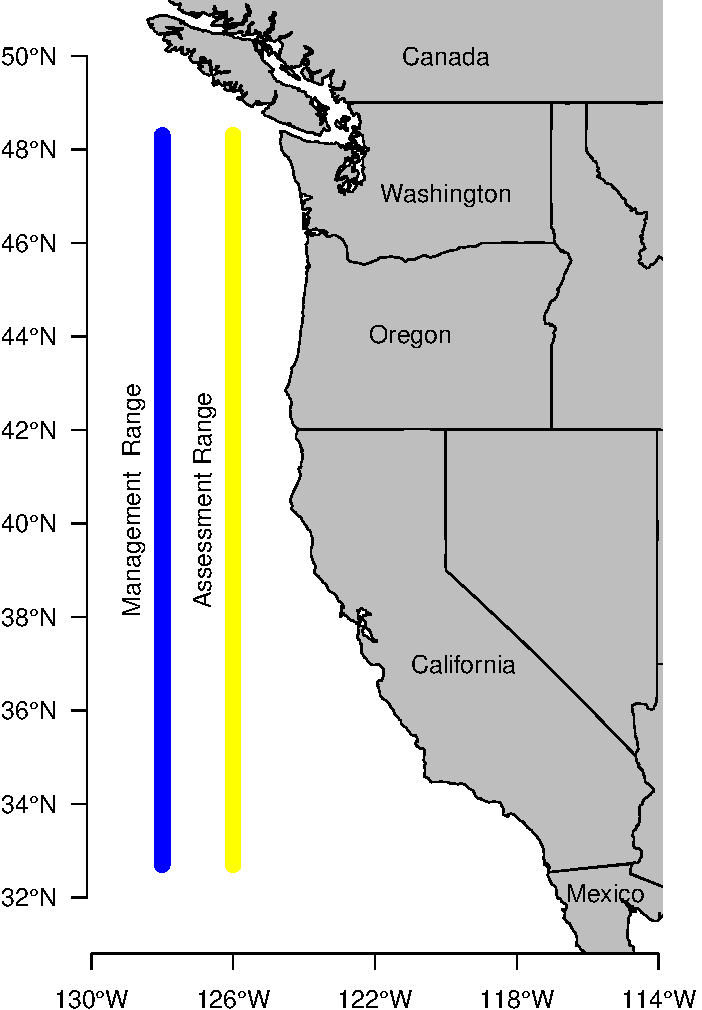
\includegraphics{SAR_USWC_Rougheye_and_Blackspotted_Rockfishes_skeleton_files/figure-pdf/fig-map-1.pdf}

}

\caption{\label{fig-map}Map of the assessment area.}

\end{figure}%

\begin{figure}[H]

\centering{

\includegraphics{plots_4_doc/cpue_map.png}

}

\caption{\label{fig-cpue-map}Rougheye/Blackspotted Rockfishes 2003-2024
WCGBTS CPUE map.}

\end{figure}%

\begin{figure}[H]

\centering{

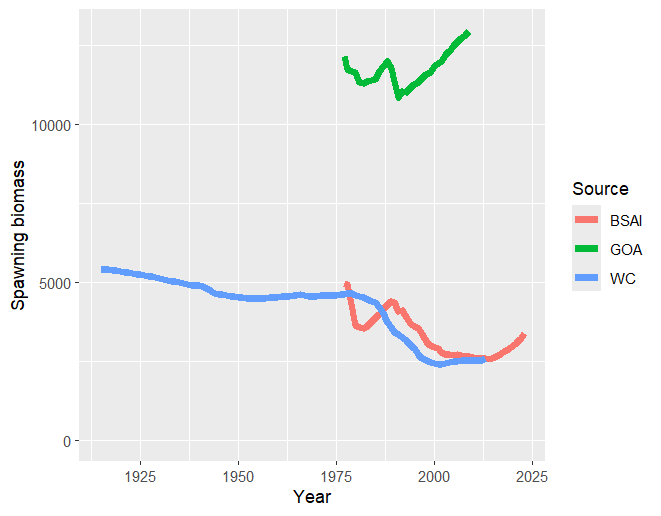
\includegraphics{plots_4_doc/SB_comps.png}

}

\caption{\label{fig-SO_comp}Estimates of biomass for the
Rougheye/Blackspotted rockfish complex from the two most recent Alaska
(Bering Sea/Aleutian Islands (BSAI) and Gulf of Alaska (GOA)) and the
2013 U.S. West Coast stock assessment.}

\end{figure}%

\begin{figure}[H]

\centering{

\includegraphics{plots_4_doc/Status_comp.png}

}

\caption{\label{fig-RSS_comp}Estimates of fraction unfished relative to
1977 (the common year in all stock assessments compared) for the
Rougheye/Blackspotted rockfish complex from the two most recent Alaska
(Bering Sea/Aleutian Islands (BSAI) and Gulf of Alaska (GOA)) and the
2013 U.S. West Coast stock assessment.}

\end{figure}%

\newpage

\subsection{Data}\label{data-2}

\begin{figure}[H]

\centering{


\includegraphics{ref_model/plots/data_plot.png}

}

\caption{\label{fig-data}Data sources by year used in the assessment.}

\end{figure}%

\begin{figure}[H]

\centering{

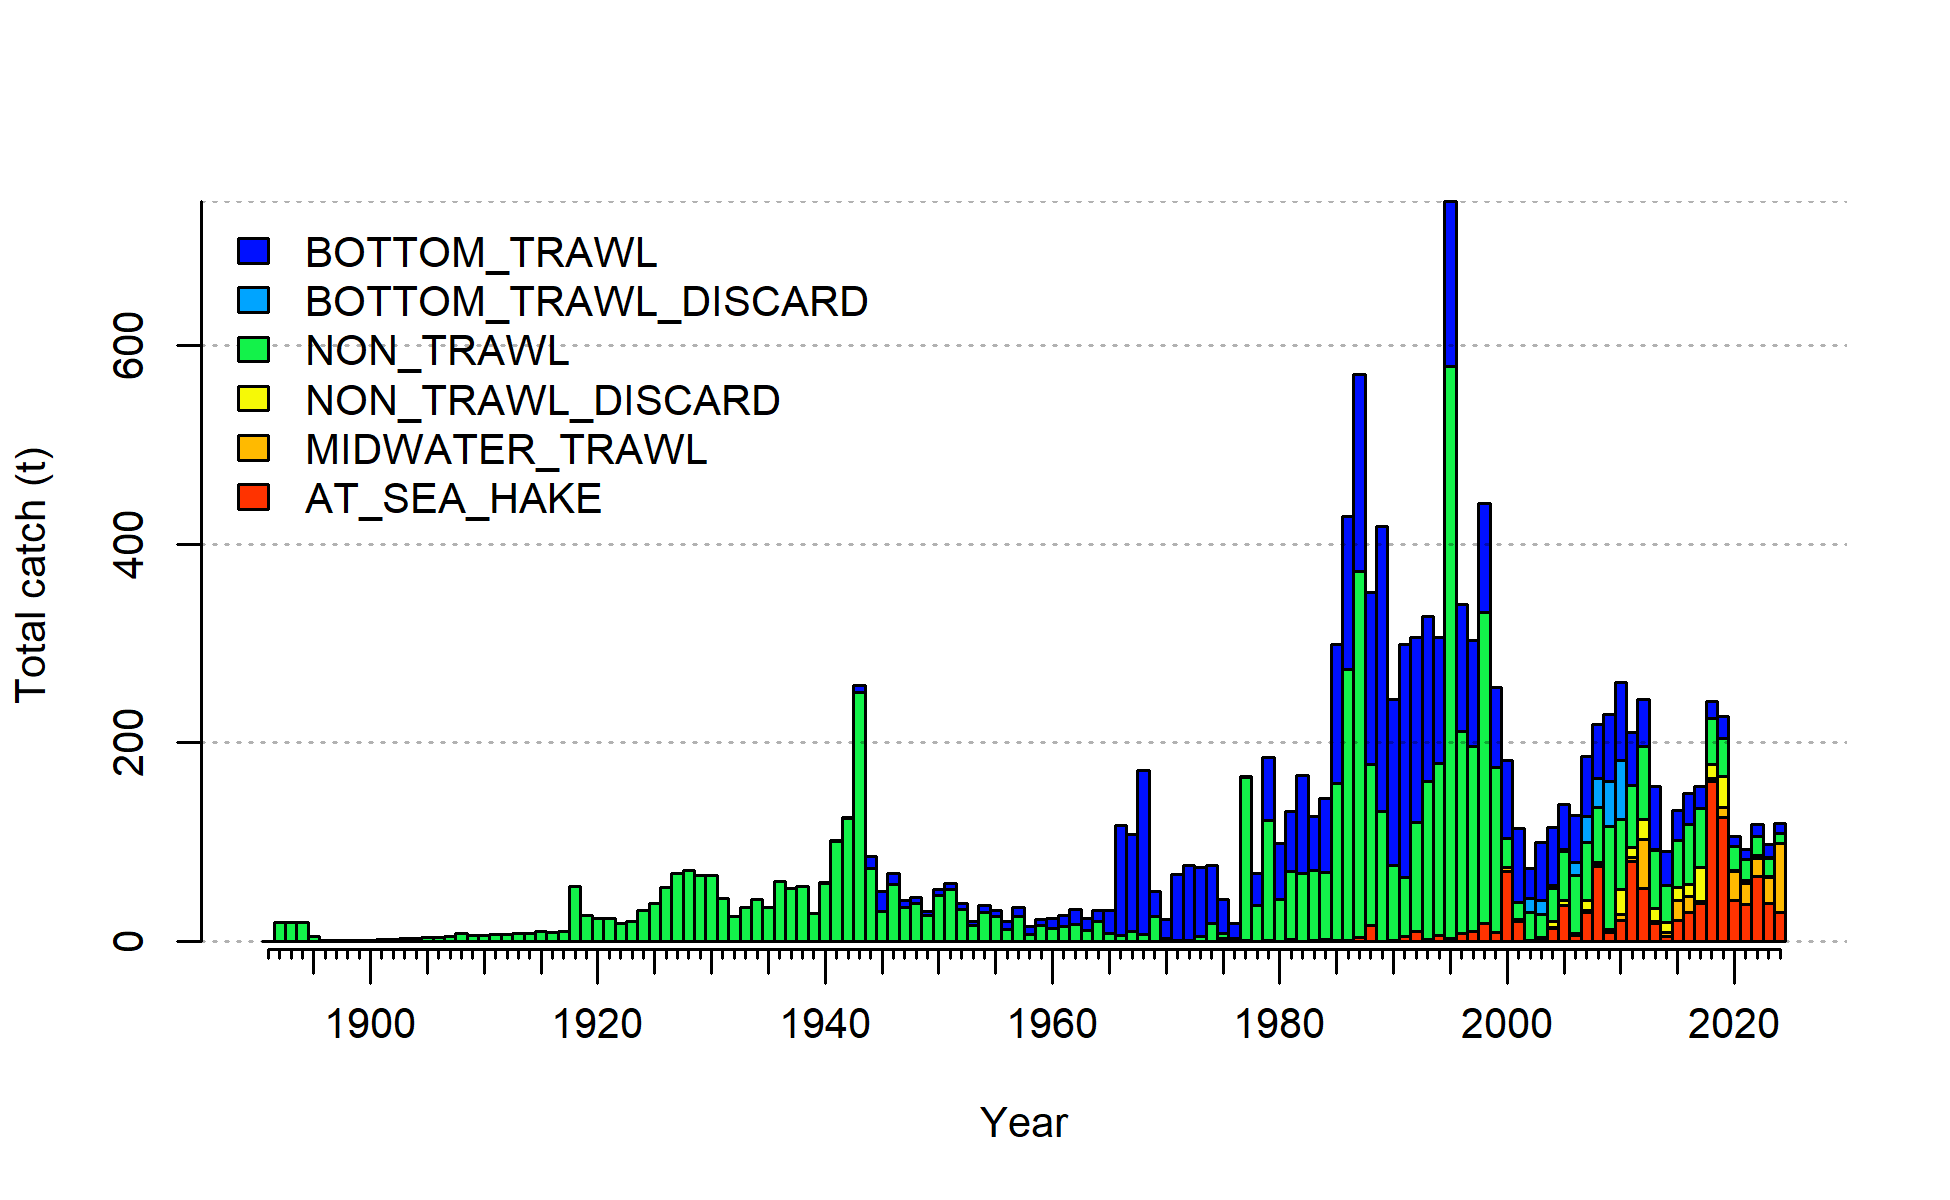
\includegraphics{ref_model/plots/catch2_landings_stacked.png}

}

\caption{\label{fig-landings}Time series of catches by fleet.}

\end{figure}%

\begin{figure}[H]

\centering{

\includegraphics{plots_4_doc/Catch_comp_all.png}

}

\caption{\label{fig-Ct_All}Landings (metric tons) across all states for
non-trawl and trawl fisheries compared between the 2013 assessment and
updated landings for the 2025 stock assessment model.}

\end{figure}%

\begin{figure}[H]

\centering{

\includegraphics{plots_4_doc/Catch_comp_CA.png}

}

\caption{\label{fig-Ct_CA}California state landings (metric tons) for
non-trawl and trawl fisheries compared between the 2013 assessment and
updated landings for the 2025 stock assessment model.}

\end{figure}%

\begin{figure}[H]

\centering{

\includegraphics{plots_4_doc/Catch_comp_OR.png}

}

\caption{\label{fig-Ct_OR}Oregon state landings (metric tons) for
non-trawl and trawl fisheries compared between the 2013 assessment and
updated landings for the 2025 stock assessment model.}

\end{figure}%

\begin{figure}[H]

\centering{

\includegraphics{plots_4_doc/Catch_comp_WA.png}

}

\caption{\label{fig-Ct_WA}Washington state landings (metric tons) for
non-trawl and trawl fisheries compared between the 2013 assessment and
updated landings for the 2025 stock assessment model.}

\end{figure}%

\begin{figure}[H]

\centering{


\includegraphics{ref_model/plots/comp_lendat_flt1mkt0_page1.png}

}

\caption{\label{fig-length_flt1_1}Length composition data for bottom
trawl fleet.}

\end{figure}%

\begin{figure}[H]

\centering{


\includegraphics{ref_model/plots/comp_lendat_flt1mkt0_page2.png}

}

\caption{\label{fig-length_flt1_2}Length composition data for bottom
trawl fleet, continued.}

\end{figure}%

\begin{figure}[H]

\centering{


\includegraphics{ref_model/plots/comp_lendat_flt2mkt0.png}

}

\caption{\label{fig-length_flt2}Length composition data for bottom trawl
discard fleet.}

\end{figure}%

\begin{figure}[H]

\centering{


\includegraphics{ref_model/plots/comp_lendat_flt3mkt0_page1.png}

}

\caption{\label{fig-length_flt3_1}Length composition data for non-trawl
fleet.}

\end{figure}%

\begin{figure}[H]

\centering{


\includegraphics{ref_model/plots/comp_lendat_flt3mkt0_page2.png}

}

\caption{\label{fig-length_flt3_2}Length composition data for non-trawl
fleet, continued.}

\end{figure}%

\begin{figure}[H]

\centering{


\includegraphics{ref_model/plots/comp_lendat_flt4mkt0.png}

}

\caption{\label{fig-length_flt4}Length composition data for non-trawl
discard fleet.}

\end{figure}%

\begin{figure}[H]

\centering{


\includegraphics{ref_model/plots/comp_lendat_flt5mkt0.png}

}

\caption{\label{fig-length_flt5}Length composition data for mid-water
trawl fleet.}

\end{figure}%

\begin{figure}[H]

\centering{


\includegraphics{ref_model/plots/comp_lendat_flt6mkt0.png}

}

\caption{\label{fig-length_flt6}Length composition data for at-sea hake
fleet.}

\end{figure}%

\begin{figure}[H]

\centering{


\includegraphics{ref_model/plots/comp_lendat_flt10mkt0.png}

}

\caption{\label{fig-length_flt10}Length composition data for the West
Coast Groundfish Bottom Trawl Survey (WCGBTS).}

\end{figure}%

\begin{figure}[H]

\centering{


\includegraphics{ref_model/plots/comp_lendat_flt7mkt0.png}

}

\caption{\label{fig-length_flt7}Length composition data for Triennial
Survey.}

\end{figure}%

\begin{figure}[H]

\centering{


\includegraphics{ref_model/plots/comp_lendat_flt8mkt0.png}

}

\caption{\label{fig-length_flt8}Length composition data for AFSC Slope
Survey.}

\end{figure}%

\begin{figure}[H]

\centering{


\includegraphics{ref_model/plots/comp_condAALdat_bubflt1mkt0_page1.png}

}

\caption{\label{fig-caal_flt1_1}Length composition data for bottom trawl
fleet.}

\end{figure}%

\begin{figure}[H]

\centering{


\includegraphics{ref_model/plots/comp_condAALdat_bubflt1mkt0_page2.png}

}

\caption{\label{fig-caal_flt1_2}Length composition data for bottom trawl
fleet, continued.}

\end{figure}%

\begin{figure}[H]

\centering{


\includegraphics{ref_model/plots/comp_condAALdat_bubflt3mkt0_page1.png}

}

\caption{\label{fig-caal_flt3_1}Conditional ages-at-length composition
data for non-trawl fleet.}

\end{figure}%

\begin{figure}[H]

\centering{


\includegraphics{ref_model/plots/comp_condAALdat_bubflt3mkt0_page2.png}

}

\caption{\label{fig-caal_flt3_2}Conditional ages-at-length composition
data for non-trawl fleet, continued.}

\end{figure}%

\begin{figure}[H]

\centering{


\includegraphics{ref_model/plots/comp_condAALdat_bubflt5mkt0.png}

}

\caption{\label{fig-caal_flt5}Conditional ages-at-length composition
data for Midwater trawl fleet.}

\end{figure}%

\begin{figure}[H]

\centering{


\includegraphics{ref_model/plots/comp_condAALdat_bubflt6mkt0_page1.png}

}

\caption{\label{fig-caal_flt6_1}Conditional ages-at-length composition
data for at-sea hake fleet.}

\end{figure}%

\begin{figure}[H]

\centering{


\includegraphics{ref_model/plots/comp_condAALdat_bubflt6mkt0_page2.png}

}

\caption{\label{fig-caal_flt6_2}Conditional ages-at-length composition
data for at-sea hake fleet, continued.}

\end{figure}%

\begin{figure}[H]

\centering{


\includegraphics{ref_model/plots/comp_condAALdat_bubflt10mkt0_page1.png}

}

\caption{\label{fig-caal_flt10_1}Conditional ages-at-length composition
data for the West Coast Groundfish Bottom Trawl Survey (WCGBTS).}

\end{figure}%

\begin{figure}[H]

\centering{


\includegraphics{ref_model/plots/comp_condAALdat_bubflt10mkt0_page2.png}

}

\caption{\label{fig-caal_flt10_2}Conditional ages-at-length composition
data for the West Coast Groundfish Bottom Trawl Survey (WCGBTS),
continued.}

\end{figure}%

\begin{figure}[H]

\centering{


\includegraphics{ref_model/plots/comp_condAALdat_bubflt10mkt0_page3.png}

}

\caption{\label{fig-caal_flt10_3}Conditional ages-at-length composition
data for the West Coast Groundfish Bottom Trawl Survey (WCGBTS),
continued.}

\end{figure}%

\begin{figure}[H]

\centering{


\includegraphics{ref_model/plots/index9_standcpueall.png}

}

\caption{\label{fig-All_indices}Standardized survey indices used in the
assessment.}

\end{figure}%

\begin{figure}[H]

\centering{

\includegraphics{plots_4_doc/WCGBTS_comps.png}

}

\caption{\label{fig-WCGBTS_comparison}Comparison of the West Coast
Groundfish Bottom Trawl Survey (WCGBTS) index from the previous
assessment (GLMM) and the WCGBTS index of abundance used in this
assessment (sdmTMB, lognormal distribution).}

\end{figure}%

\begin{figure}[H]

\centering{


\includegraphics{ref_model/plots/index1_cpuedata_WCGBTS.png}

}

\caption{\label{fig-WCGBTS_index}West Coast Groundfish Bottom Trawl
Survey (WCGBTS) index.}

\end{figure}%

\begin{figure}[H]

\centering{


\includegraphics{ref_model/plots/index1_cpuedata_TRIENNIAL.png}

}

\caption{\label{fig-Triennial_index}Triennial Survey index.}

\end{figure}%

\begin{figure}[H]

\centering{


\includegraphics{ref_model/plots/index1_cpuedata_AK_SLOPE.png}

}

\caption{\label{fig-AFSC_Slope_index}AFSC Slope Survey index.}

\end{figure}%

\begin{figure}[H]

\centering{


\includegraphics{ref_model/plots/index1_cpuedata_NW_SLOPE.png}

}

\caption{\label{fig-NWFSC_Slope_index}NWFSC Slope Survey index.}

\end{figure}%

\begin{figure}[H]

\centering{

\includegraphics{plots_4_doc/compare1_spawnbio_updatedCt.png}

}

\caption{\label{fig-Ct_compsSO}Comparison of spawning biomass between
2013 Rougheye/Blackspotted Rockfishes assessment model and model with
updated/extended catches used in 2025 assessment.}

\end{figure}%

\begin{figure}[H]

\centering{

\includegraphics{plots_4_doc/compare3_Bratio_updatedCt.png}

}

\caption{\label{fig-Ct_compsRSS}Comparison of fraction unfished between
2013 Rougheye/Blackspotted Rockfishes assessment model and model with
updated/extended catches used in 2025 assessment.}

\end{figure}%

\newpage

\subsection{Biology}\label{biology}

\begin{figure}[H]

\centering{

\includegraphics{plots_4_doc/1v2sex_spawnbio.png}

}

\caption{\label{fig-Sex1vs2_SO}Comparison of spawning biomass using the
1 sex and 2 sexes set to equal values models based on the 2013
Rougheye/Blackspotted Rockfishes assessment data. The 1 sex model has
double the biomass because it includes both females and males.}

\end{figure}%

\begin{figure}[H]

\centering{

\includegraphics{plots_4_doc/1v2sex_Bratio_uncertainty.png}

}

\caption{\label{fig-Sex1vs2_Bratio}Comparison of fraction unfished using
the 1 sex and 2 sexes set to equal values models based on the 2013
Rougheye/Blackspotted Rockfishes assessment data.}

\end{figure}%

\begin{figure}[H]

\centering{

\includegraphics{plots_4_doc/M_values.png}

}

\caption{\label{fig-Mcurves}Natural mortality curves by age in years for
values of natural mortality used in various Rougheye/Blackspotted
Rockfish stock assessments. Dots indicate the range of assumed maximum
ages using the equation from Hamel and Cope 2022.}

\end{figure}%

\begin{figure}[H]

\centering{

\includegraphics{plots_4_doc/Catch_curve_plot_FM.png}

}

\caption{\label{fig-CC_Z}Catch curve (log abundance by age) analysis on
aggregated ages over all age sources by sex (black points). The peak
selected age was 21 for both sexes, so the linear model was run from age
21 until the oldest age (red points). The slope of the linear model is
equal to the estimate of an aggregate total mortality (Z).}

\end{figure}%

\begin{figure}[H]

\centering{

\includegraphics{plots_4_doc/Catch_curve_plot_FM_21_100.png}

}

\caption{\label{fig-CC_Z_100}Catch curve (log abundance by age) analysis
on aggregated ages over all age sources by sex (black points). The peak
selected age was 21 for both sexes with a max age of 100, so the linear
model was run from age 21 until age 100 (red points). The slope of the
linear model is equal to the estimate of an aggregate total mortality
(Z).}

\end{figure}%

\begin{figure}[H]

\centering{

\includegraphics{plots_4_doc/Catch_curve_plot_FM_21_80.png}

}

\caption{\label{fig-CC_Z_80}Catch curve (log abundance by age) analysis
on aggregated ages over all age sources by sex (black points). The peak
selected age was 21 for both sexes with a max age of 80, so the linear
model was run from age 21 until age 80 (red points). The slope of the
linear model is equal to the estimate of an aggregate total mortality
(Z).}

\end{figure}%

\begin{figure}[H]

\centering{

\includegraphics{plots_4_doc/Age_length_plot.png}

}

\caption{\label{fig-AL_1}Age and length data, with fitted von
Bertalanffy growth curves, by sex and data source for the
Rougheye/Blackspotted rockfish complex. Sample sizes (N) are also
provided.}

\end{figure}%

\begin{figure}[H]

\centering{

\includegraphics{plots_4_doc/Lt_age_CV_FM.png}

}

\caption{\label{fig-AL_2}Coefficient of variation by age and sex for all
sources of Rougheye/Blackspotted rockfishes ages. Sample sizes (N) are
also indicated by size of the point. The line is a smoothed loess
(polynomial) line that gives a moving average of CV by age and sex.}

\end{figure}%

\begin{figure}[H]

\centering{

\includegraphics{plots_4_doc/AE_matrix_plot.png}

}

\caption{\label{fig-AE_matrices}Ageing error matrix assignments by year
and data source. The number indicates which ageing error matrix was used
for conditional ages within those years and data sources. `Commercial'
is a combination of all commercial fleets.}

\end{figure}%

\begin{figure}[H]

\centering{

\includegraphics{plots_4_doc/AE_Bias.png}

}

\caption{\label{fig-AE_bias}Estimated bias used for each of the seven
ageing error matrices.}

\end{figure}%

\begin{figure}[H]

\centering{

\includegraphics{plots_4_doc/AE_SD.png}

}

\caption{\label{fig-AE_SD}Estimated imprecision (as a standard
deviation) used for each of the seven ageing error matrices.}

\end{figure}%

\newpage

\begin{figure}[H]

\centering{

\includegraphics{plots_4_doc/L_W_plots.png}

}

\caption{\label{fig-LW1}Length and weight samples by sex and data
source. Lines are the power function fits by data source.}

\end{figure}%

\begin{figure}[H]

\centering{

\includegraphics{plots_4_doc/F_M_ltwt_plot.png}

}

\caption{\label{fig-LW2}Realized length and weight relationships for
female and male Rougheye/Blackspotted Rockfishes.}

\end{figure}%

\newpage

\begin{figure}[H]

\centering{

\includegraphics{plots_4_doc/bio_fxn_maturity.png}

}

\caption{\label{fig-maturity_bio_fxn}Proportion of mature fish by length
when using biological versus functional maturity criteria.}

\end{figure}%

\begin{figure}[H]

\centering{

\includegraphics{plots_4_doc/l50_both_species.png}

}

\caption{\label{fig-maturity_length_both}Proportion of mature fish by
length for the Rougheye/Blackspotted rockfishes complex and by species.}

\end{figure}%

\begin{figure}[H]

\centering{

\includegraphics{plots_4_doc/a50_both_species.png}

}

\caption{\label{fig-maturity_age_both}Proportion of mature fish by age
for the Rougheye/Blackspotted rockfishes complex and by species.}

\end{figure}%

\newpage

\begin{figure}[H]

\centering{

\includegraphics{plots_4_doc/Bimodal_lengths_Peter_Frey.png}

}

\caption{\label{fig-bimodal-lengths}Length distribution of Rougheye
Rockfish and Blackspotted Rockfish identified to species using genetics
(pers. comm. P. Frey, NWFSC).}

\end{figure}%

\subsection{Model Bridging}\label{model-bridging}

\begin{figure}[H]

\centering{


\includegraphics{plots_4_doc/compare4_Bratio_uncertainty.png}

}

\caption{\label{fig-RSS_2013}Estimates of relative stock size (current
spawning output/unfished spawning output) for the Rougheye/Blackspotted
rockfish complex in U.S. west coast waters from the 2013 assessment, and
compared to the using the same data in the newest version of SS3
(3.30.22.2).}

\end{figure}%

\begin{figure}[H]

\centering{


\includegraphics{plots_4_doc/compare2_spawnbio_uncertainty.png}

}

\caption{\label{fig-SO_2013}Estimates of spawning biomass for the
Rougheye/Blackspotted rockfish complex in U.S. west coast waters from
the 2013 assessment, and compared to the same data in the newest version
of SS3 (3.30.22.2). Shading denotes 95\% confidence intervals. Shading
denotes 95\% confidence intervals.}

\end{figure}%

\begin{figure}[H]

\centering{

\includegraphics{plots_4_doc/compare1_spawnbio__discard_fleets.png}

}

\caption{\label{fig-Discard_comp_SO}Comparison of spawning biomass using
retention curves or discard fleets using the 2013 Rougheye/Blackspotted
Rockfishes assessment.}

\end{figure}%

\begin{figure}[H]

\centering{

\includegraphics{plots_4_doc/compare3_Bratio_discard_fleets.png}

}

\caption{\label{fig-Discard_comp_RSS}Comparison of fraction unfished
(relative spawning biomass) using retention curves or discard fleets
using the 2013 Rougheye/Blackspotted Rockfishes assessment.}

\end{figure}%

\begin{figure}[H]

\centering{

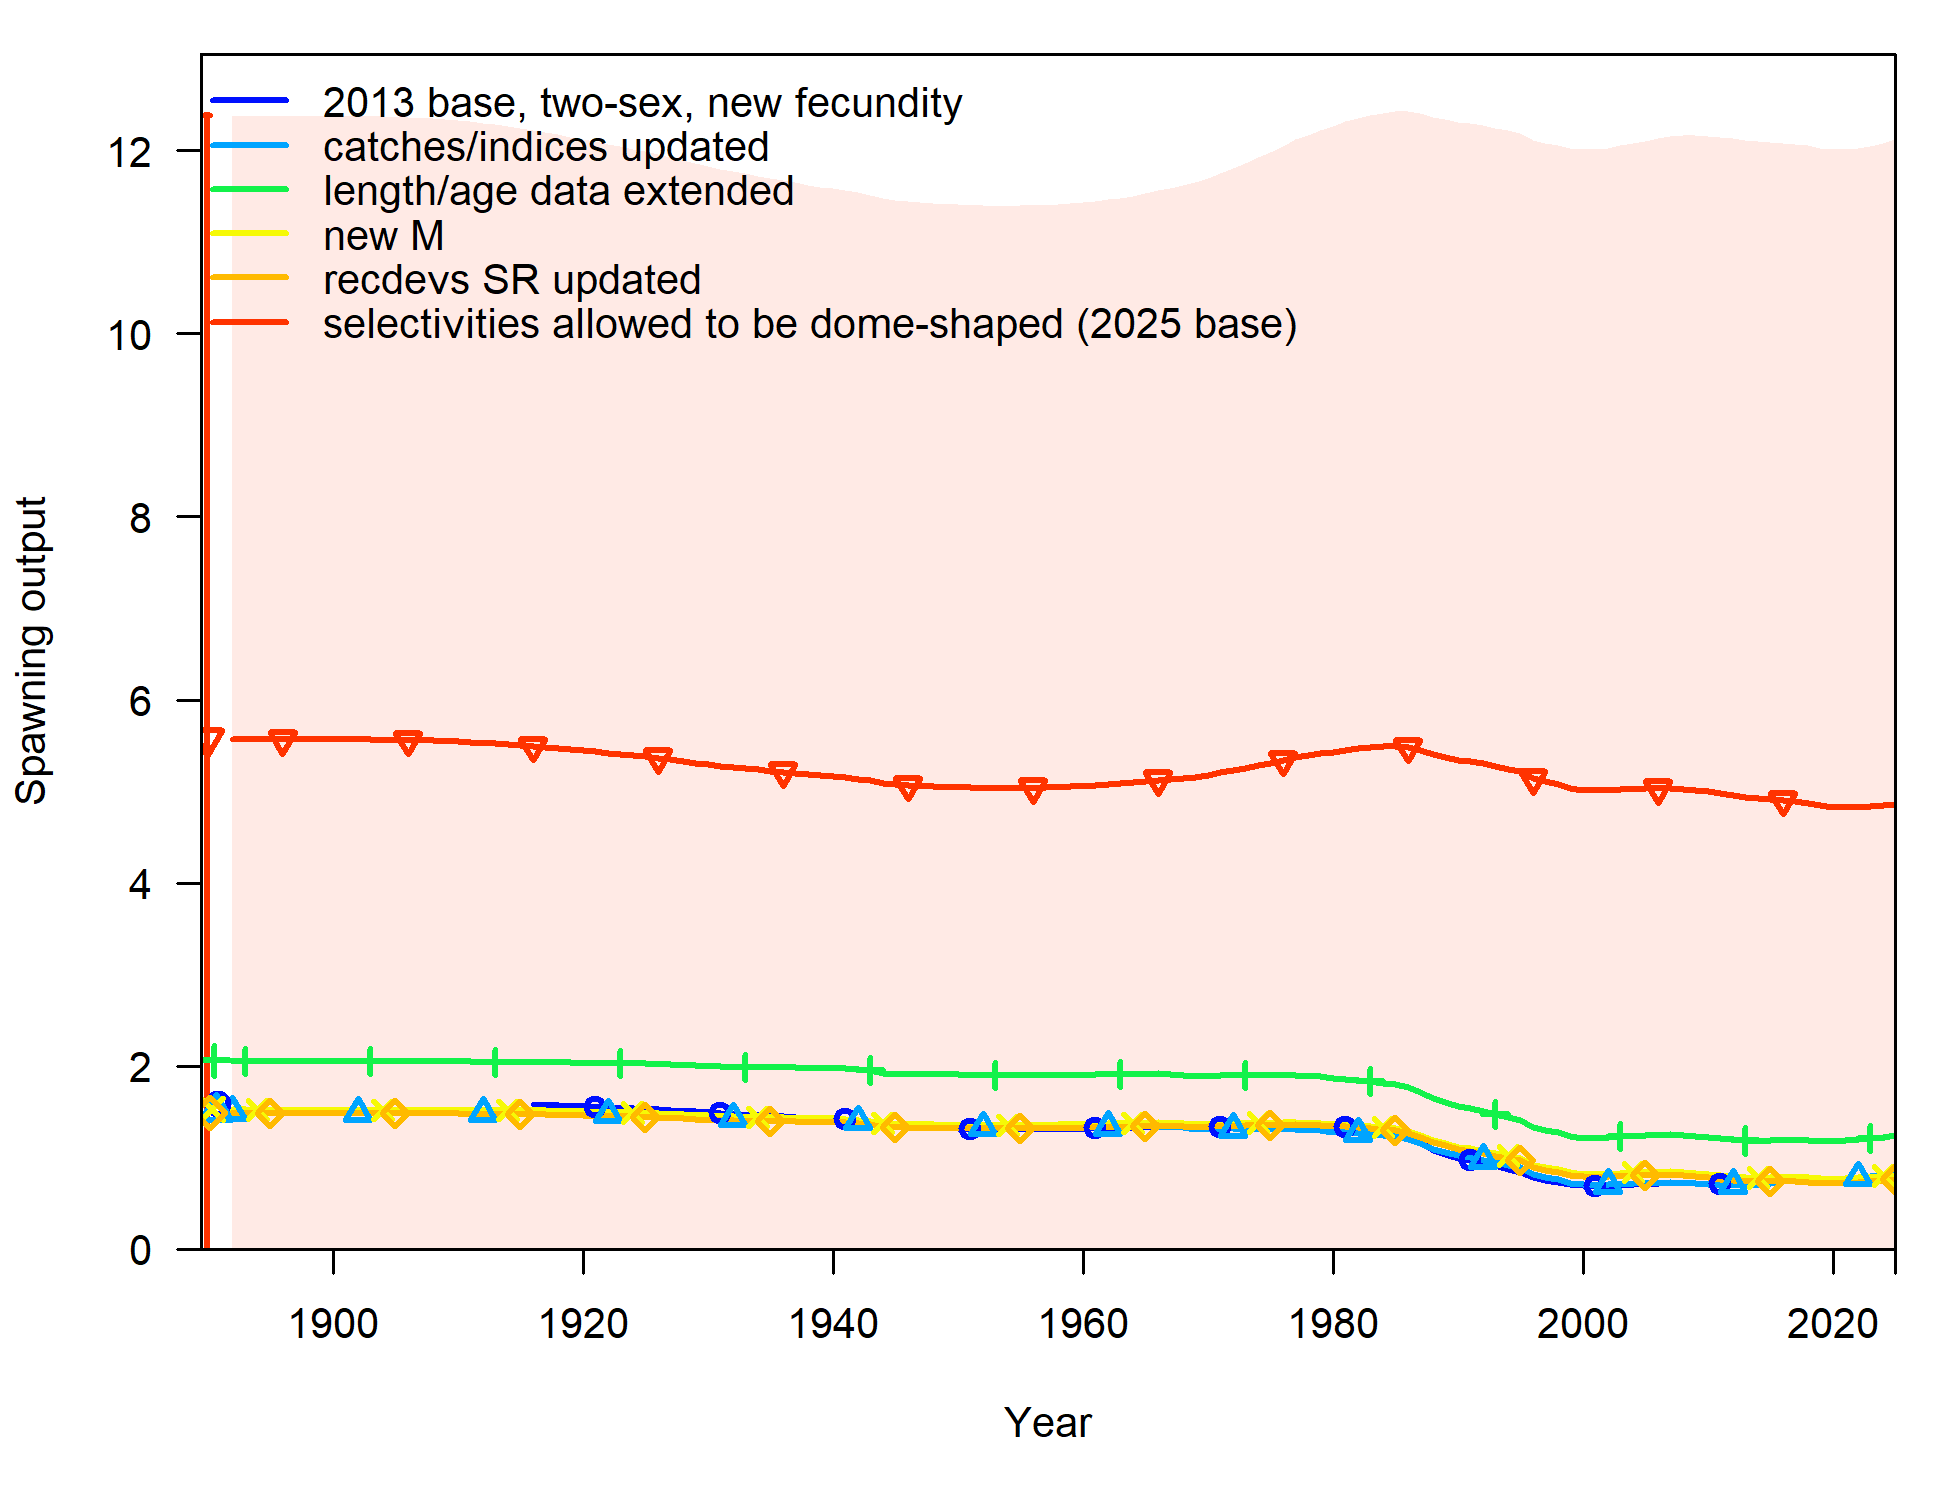
\includegraphics{plots_4_doc/bridging_compare2_spawnbio_uncertainty.png}

}

\caption{\label{fig-SO_Bridging}Time series of estimated spawning output
(trillions of eggs) for bridging analysis.}

\end{figure}%

\begin{figure}[H]

\centering{

\includegraphics{plots_4_doc/bridging_compare4_Bratio_uncertainty.png}

}

\caption{\label{fig-Bratio_Bridging}Time series of fraction of unfished
spawning output for bridging analysis.}

\end{figure}%

\begin{figure}[H]

\centering{

\includegraphics{plots_4_doc/NT_length_vs_discard.png}

}

\caption{\label{fig-NT-lengths-for-blocks}Comparison of length
compositions (lengths in cm) between non-trawl and non-trawl discard
fleets, sexes combined.}

\end{figure}%

\begin{figure}[H]

\centering{

\includegraphics{plots_4_doc/Trawl_landings_discard_comparisons.png}

}

\caption{\label{fig-BT-lengths-for-blocks}Comparison of length
compositions (lengths in cm) between trawl and trawl discard fleets,
sexes combined.}

\end{figure}%

\newpage

\subsection{Model Diagnostics}\label{model-diagnostics-1}

\begin{figure}[H]

\centering{

\includegraphics{plots_4_doc/piner_panel_NatM_uniform_Mal_GP_1.png}

}

\caption{\label{fig-M-profile-explore}Likelihood profile and component
likelihoods used to establish a fixed value for male natural mortality.}

\end{figure}%

\newpage

\begin{figure}[H]

\centering{

\includegraphics{plots_4_doc/Sensi_logREplot_status_LAO.png}

}

\caption{\label{fig-LAO-mod-comps}Log relative change
(log((Model\_sensi-Model\_ref)/Model\_ref)) in length and/or age only
scenarios for relative stock status. Box indicates 95 percent confidence
interval of the reference model.}

\end{figure}%

\newpage

\subsection{Model Convergence}\label{model-convergence}

\begin{figure}[H]

\centering{

\includegraphics{plots_4_doc/pairs_plot_fast.png}

}

\caption{\label{fig-pairs_plot_fast}Pairs plots of the fastest mixing
parameters from running 2000 posterior draws (keeping every draw) using
the random walk Metropolis algorithm. Parameters that show little to no
movement are recommended to be fixed to improve model speed and
efficiency.}

\end{figure}%

\begin{figure}[H]

\centering{


\includegraphics{ref_model/Jitter Results_0.01/jitterplot.png}

}

\caption{\label{fig-jitter001}Jitter runs (using a value of 0.01) for
the reference model, with jitter run number on the x-axis and -log
likelihood value on the y-axis. Blue dot are models that match the
likelihood value of the reference model, while red dots deviate from the
reference model. All red dots are above the blue dots, indicating no
better fit to the reference model was found.}

\end{figure}%

\begin{figure}[H]

\centering{


\includegraphics{ref_model/Jitter Results_0.05/jitterplot.png}

}

\caption{\label{fig-jitter005}Jitter runs (using a value of 0.05) for
the reference model, with jitter run number on the x-axis and -log
likelihood value on the y-axis. Blue dot are models that match the
likelihood value of the reference model, while red dots deviate from the
reference model. All red dots are above the blue dots, indicating no
better fit to the reference model was found.}

\end{figure}%

\newpage

\subsection{Retrospecitve Analysis}\label{retrospecitve-analysis}

\begin{figure}[H]

\centering{


\includegraphics{Retros/compare2_spawnbio_uncertainty.png}

}

\caption{\label{fig-retro-so}Change in the estimate of spawning output
(quadrillions of eggs) when the five most recent years of data area
removed sequentially.}

\end{figure}%

\begin{figure}[H]

\centering{


\includegraphics{Retros/compare4_Bratio_uncertainty.png}

}

\caption{\label{fig-retro-status}Change in the estimate of relative
stock status (fraction unfished) when the five most recent years of data
area removed sequentially.}

\end{figure}%

\begin{figure}[H]

\centering{


\includegraphics{Like_profiles/ref_model_retro_2_yr_peel/compare2_spawnbio_uncertainty.png}

}

\caption{\label{fig-retro-scale-12}Change in the estimate of spawning
output (quadrillions of eggs) when the two most recent years of data
area removed sequentially. Uncertainty envelopes are also provided for
the reference model.}

\end{figure}%

\begin{figure}[H]

\centering{

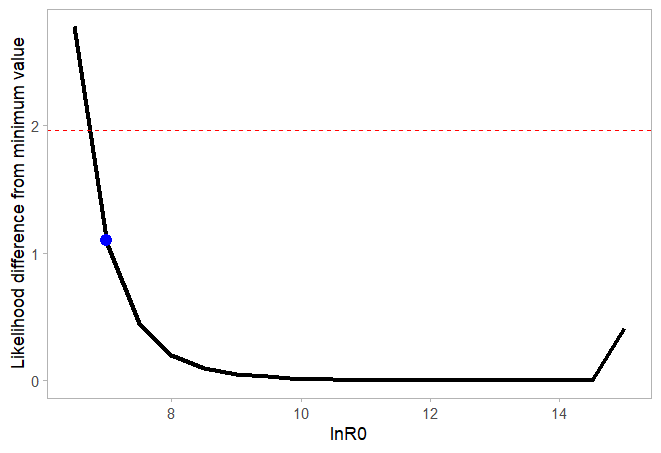
\includegraphics{Like_profiles/Retro3_like_diff.png}

}

\caption{\label{fig-retro-minus3-scale}Initial recruitment (\(lnR_0\))
likelihood profile (change in the negative log-likelihood across a range
of \(lnR0\) values) and derived quantities for the retrospective -3
years model. Red line in the top left figure indicates the significance
level in likelihood difference. Blue dot is the reference model value.}

\end{figure}%

\begin{figure}[H]

\centering{

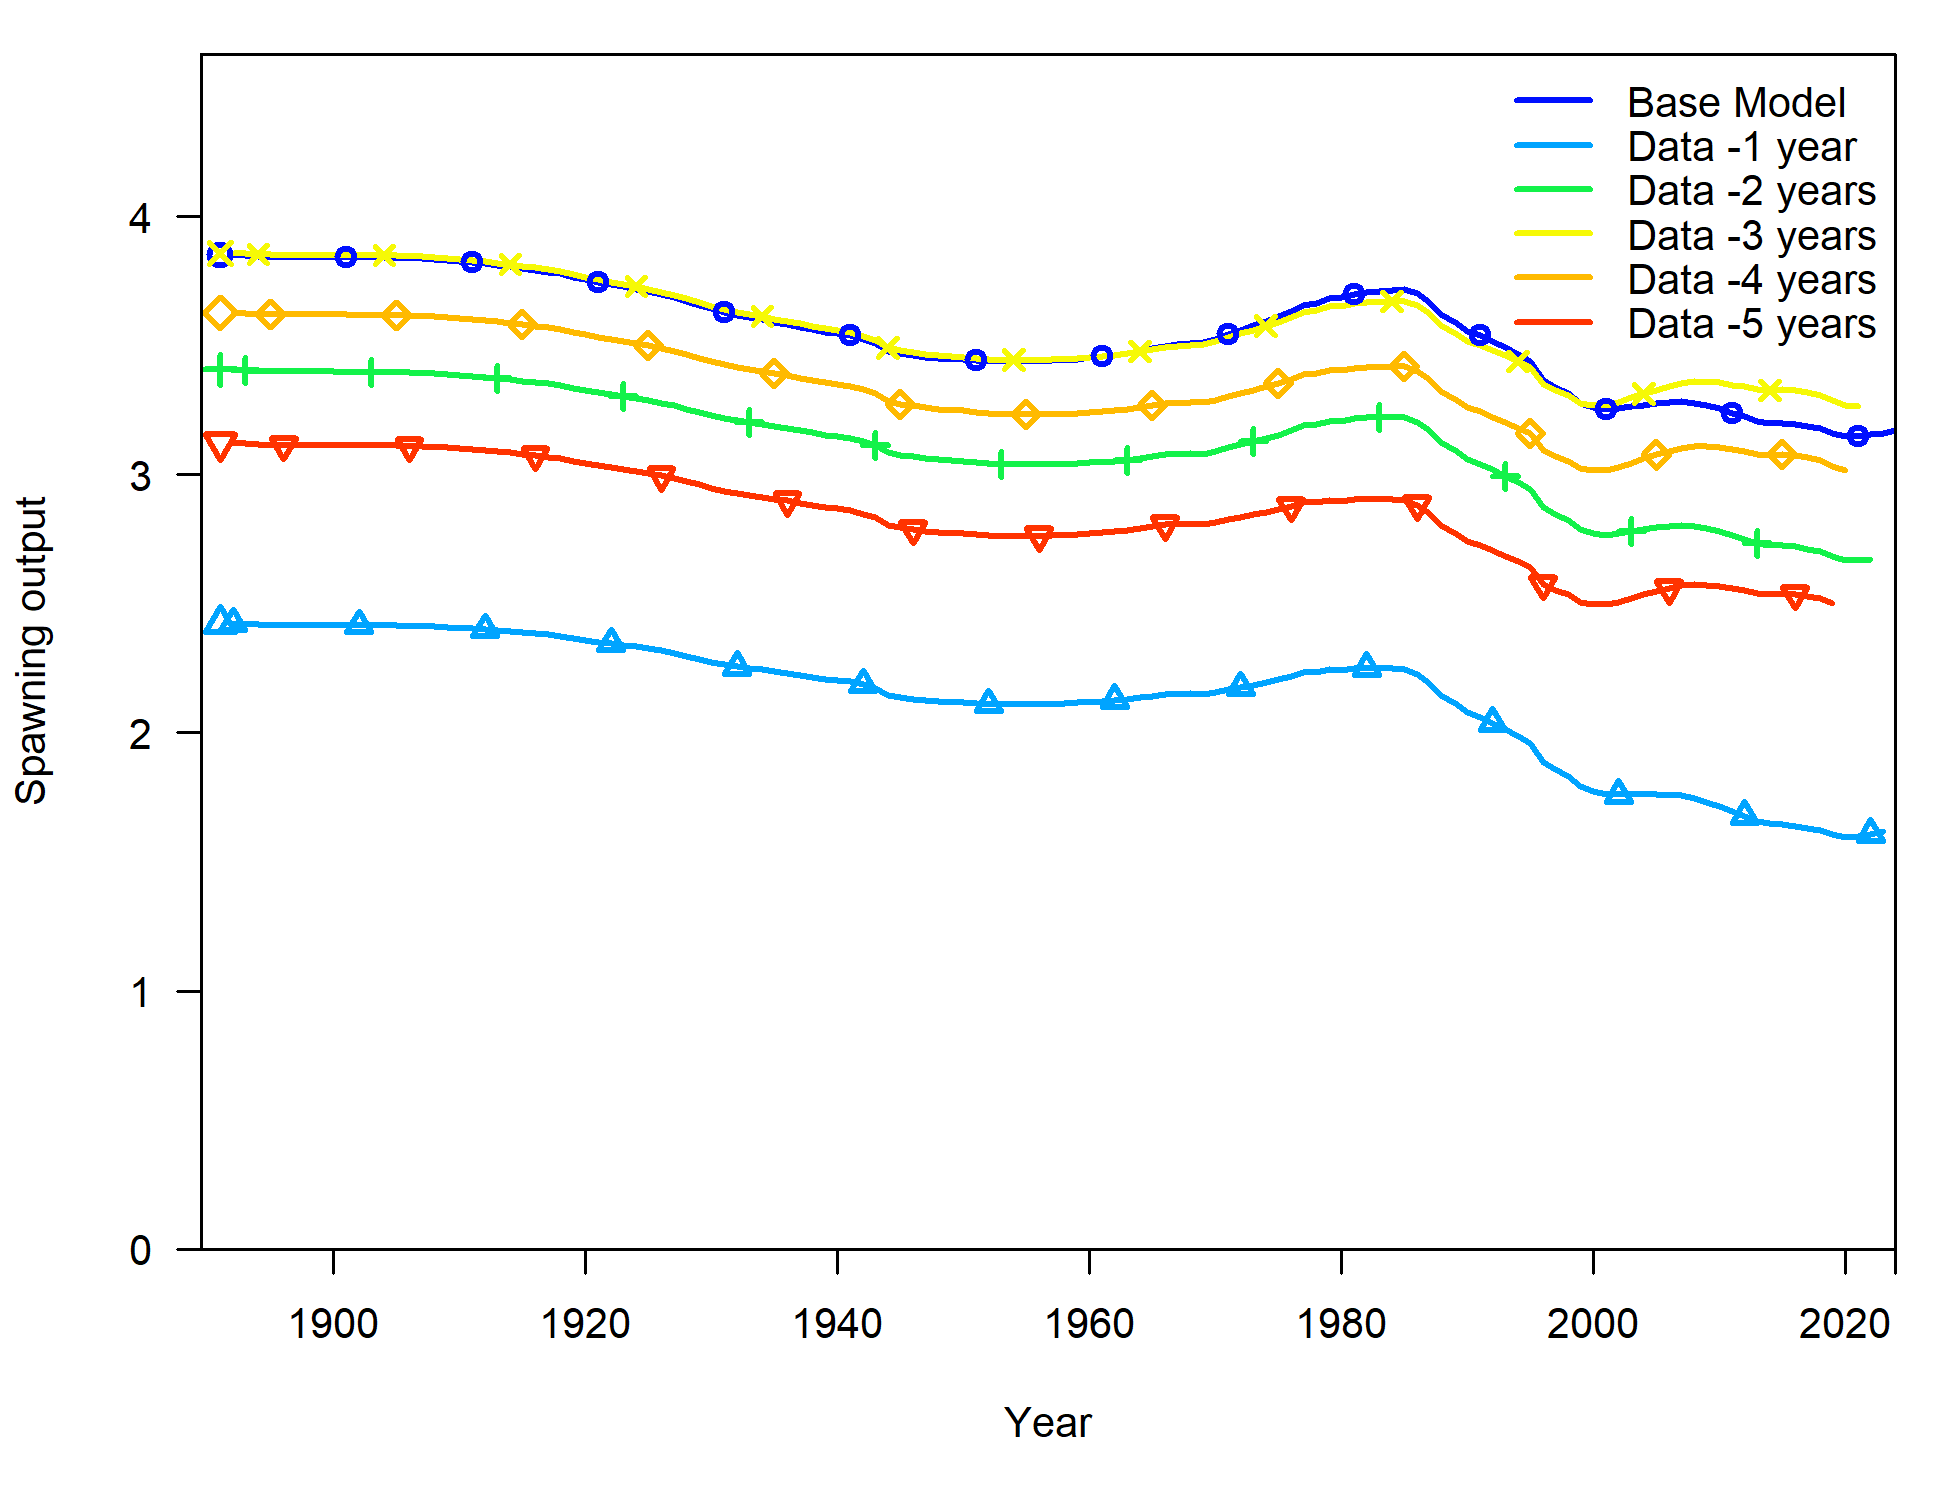
\includegraphics{plots_4_doc/No_block_retro_compare1_spawnbio.png}

}

\caption{\label{fig-noblock_retro}Change in the estimate of spawning
output (trillions of eggs) when the five most recent years of data area
removed sequentially in the model with the most recent block on
non-trawl fleet selelctivity extended to start in 2011 (instead of
2020). Base model in this plot labels the model with modified block, not
the assessment base model.}

\end{figure}%

\newpage

\subsection{Model Fits to Data}\label{model-fits-to-data}

\subsubsection{Lengths}\label{lengths-1}

\begin{figure}[H]

\centering{


\includegraphics{ref_model/plots/comp_lenfit__aggregated_across_time.png}

}

\caption{\label{fig-agg-len-fit}Model fit to aggregated length (cm)
compositions over all years.}

\end{figure}%

\begin{figure}[H]

\centering{


\includegraphics{ref_model/plots/comp_lenfit_flt1mkt0_page1.png}

}

\caption{\label{fig-len-fit-bt-1}Observed (gray density plot) and
expected (density lines by sex) length compositions by year for the
bottom trawl fishery in years available between 1995-2018.'N adj.' is
the input sample size after data-weighting adjustment. N eff. is the
calculated effective sample size used in the McAllister-Ianelli tuning
method.}

\end{figure}%

\begin{figure}[H]

\centering{


\includegraphics{ref_model/plots/comp_lenfit_flt1mkt0_page2.png}

}

\caption{\label{fig-len-fit-bt-2}Observed (gray density plot) and
expected (density lines by sex) length compositions by year for the
bottom trawl fishery in years available between 2019-2024.'N adj.' is
the input sample size after data-weighting adjustment. N eff. is the
calculated effective sample size used in the McAllister-Ianelli tuning
method.}

\end{figure}%

\begin{figure}[H]

\centering{


\includegraphics{ref_model/plots/comp_lenfit_flt2mkt0.png}

}

\caption{\label{fig-len-fit-btdis}Observed (gray density plot) and
expected (density lines) length compositions by year for the bottom
trawl discard fishery in years available between 2004-2023.'N adj.' is
the input sample size after data-weighting adjustment. N eff. is the
calculated effective sample size used in the McAllister-Ianelli tuning
method.}

\end{figure}%

\begin{figure}[H]

\centering{


\includegraphics{ref_model/plots/comp_lenfit_flt3mkt0_page1.png}

}

\caption{\label{fig-len-fit-nt-1}Observed (gray density plot) and
expected (density lines by sex) length compositions by year for the
non-trawl fishery in years available between 1996-2020.'N adj.' is the
input sample size after data-weighting adjustment. N eff. is the
calculated effective sample size used in the McAllister-Ianelli tuning
method.}

\end{figure}%

\begin{figure}[H]

\centering{


\includegraphics{ref_model/plots/comp_lenfit_flt3mkt0_page2.png}

}

\caption{\label{fig-len-fit-nt-2}Observed (gray density plot) and
expected (density lines by sex) length compositions by year for the
non-trawl fishery in years available between 2021-2024.'N adj.' is the
input sample size after data-weighting adjustment. N eff. is the
calculated effective sample size used in the McAllister-Ianelli tuning
method.}

\end{figure}%

\begin{figure}[H]

\centering{


\includegraphics{ref_model/plots/comp_lenfit_flt4mkt0.png}

}

\caption{\label{fig-len-fit-ntdis}Observed (gray density plot) and
expected (density lines) length compositions by year for the midwater
trawl fishery in years available between 2004-2024.'N adj.' is the input
sample size after data-weighting adjustment. N eff. is the calculated
effective sample size used in the McAllister-Ianelli tuning method.}

\end{figure}%

\begin{figure}[H]

\centering{


\includegraphics{ref_model/plots/comp_lenfit_flt5mkt0.png}

}

\caption{\label{fig-len-fit-midt}Observed (gray density plot) and
expected (density lines by sex) length compositions by year for the
non-trawl discard fishery in years available between 2000-2023.'N adj.'
is the input sample size after data-weighting adjustment. N eff. is the
calculated effective sample size used in the McAllister-Ianelli tuning
method.}

\end{figure}%

\begin{figure}[H]

\centering{


\includegraphics{ref_model/plots/comp_lenfit_flt6mkt0.png}

}

\caption{\label{fig-len-fit-ashop}Observed (gray density plot) and
expected (density lines by sex) length compositions by year for the
at-sea-hake fishery in years available between 2003-2024.'N adj.' is the
input sample size after data-weighting adjustment. N eff. is the
calculated effective sample size used in the McAllister-Ianelli tuning
method.}

\end{figure}%

\begin{figure}[H]

\centering{


\includegraphics{ref_model/plots/comp_lenfit_flt7mkt0.png}

}

\caption{\label{fig-len-fit-tri}Observed (gray density plot) and
expected (density lines by sex) length compositions by year for the
Triennial Bottom Trawl Survey in years available between 1980-2004.'N
adj.' is the input sample size after data-weighting adjustment. N eff.
is the calculated effective sample size used in the McAllister-Ianelli
tuning method.}

\end{figure}%

\begin{figure}[H]

\centering{


\includegraphics{ref_model/plots/comp_lenfit_flt8mkt0.png}

}

\caption{\label{fig-len-fit-akslope}Observed (gray density plot) and
expected (density lines by sex) length compositions by year for the
Alaskan Slope Bottom Trawl Survey in years available between
1997-2001.'N adj.' is the input sample size after data-weighting
adjustment. N eff. is the calculated effective sample size used in the
McAllister-Ianelli tuning method.}

\end{figure}%

\begin{figure}[H]

\centering{


\includegraphics{ref_model/plots/comp_lenfit_flt10mkt0.png}

}

\caption{\label{fig-len-fit-wcgbts}Observed (gray density plot) and
expected (density lines by sex) length compositions by year for the West
Coast Groundfish Bottom Trawl Survey in years available between
1980-2004.'N adj.' is the input sample size after data-weighting
adjustment. N eff. is the calculated effective sample size used in the
McAllister-Ianelli tuning method.}

\end{figure}%

\begin{figure}[H]

\centering{


\includegraphics{ref_model/plots/comp_lenfit__page1_multi-fleet_comparison.png}

}

\caption{\label{fig-peasrson-resids-fishery}Pearson residuals of length
fits for each fishing fleet. Closed bubble are positive residuals
(observed \textgreater{} expected) and open bubbles are negative
residuals (observed \textless{} expected).}

\end{figure}%

\begin{figure}[H]

\centering{


\includegraphics{ref_model/plots/comp_lenfit__page2_multi-fleet_comparison.png}

}

\caption{\label{fig-peasrson-resids-survey}Pearson residuals of length
fits for each survey. Closed bubble are positive residuals (observed
\textgreater{} expected) and open bubbles are negative residuals
(observed \textless{} expected).}

\end{figure}%

\begin{figure}[H]

\centering{


\includegraphics{ref_model/plots/comp_lenfit_data_weighting_TA1-8_BOTTOM_TRAWL.png}

}

\caption{\label{fig-meanlt-bt}Mean length (cm) index from the bottom
trawl fishery with 95 percent confidence intervals based on sample sizes
and data weighting.}

\end{figure}%

\begin{figure}[H]

\centering{


\includegraphics{ref_model/plots/comp_lenfit_data_weighting_TA1-8_BOTTOM_TRAWL_DISCARD.png}

}

\caption{\label{fig-meanlt-btdis}Mean length (cm) index from the bottom
trawl discard fishery with 95 percent confidence intervals based on
sample sizes and data weighting.}

\end{figure}%

\begin{figure}[H]

\centering{


\includegraphics{ref_model/plots/comp_lenfit_data_weighting_TA1-8_NON_TRAWL.png}

}

\caption{\label{fig-meanlt-nt}Mean length (cm) index from the non-trawl
fishery with 95 percent confidence intervals based on sample sizes and
data weighting.}

\end{figure}%

\begin{figure}[H]

\centering{


\includegraphics{ref_model/plots/comp_lenfit_data_weighting_TA1-8_NON_TRAWL_DISCARD.png}

}

\caption{\label{fig-meanlt-ntdis}Mean length (cm) index from the
non-trawl discard fishery with 95 percent confidence intervals based on
sample sizes and data weighting.}

\end{figure}%

\begin{figure}[H]

\centering{


\includegraphics{ref_model/plots/comp_lenfit_data_weighting_TA1-8_MIDWATER_TRAWL.png}

}

\caption{\label{fig-meanlt-midt}Mean length (cm) index from the midwater
trawl fishery with 95 percent confidence intervals based on sample sizes
and data weighting.}

\end{figure}%

\begin{figure}[H]

\centering{


\includegraphics{ref_model/plots/comp_lenfit_data_weighting_TA1-8_AT_SEA_HAKE.png}

}

\caption{\label{fig-meanlt-ashop}Mean length (cm) index from the
at-sea-hake fishery with 95 percent confidence intervals based on sample
sizes and data weighting.}

\end{figure}%

\begin{figure}[H]

\centering{


\includegraphics{ref_model/plots/comp_lenfit_data_weighting_TA1-8_TRIENNIAL.png}

}

\caption{\label{fig-meanlt-tri}Mean length (cm) index from the Triennial
survey with 95 percent confidence intervals based on sample sizes and
data weighting.}

\end{figure}%

\begin{figure}[H]

\centering{


\includegraphics{ref_model/plots/comp_lenfit_data_weighting_TA1-8_AK_SLOPE.png}

}

\caption{\label{fig-meanlt-akslope}Mean length (cm) index from the
Alaskan slope survey with 95 percent confidence intervals based on
sample sizes and data weighting.}

\end{figure}%

\begin{figure}[H]

\centering{


\includegraphics{ref_model/plots/comp_lenfit_data_weighting_TA1-8_WCGBTS.png}

}

\caption{\label{fig-meanlt-wcgbts}Mean length (cm) index from the West
Coast Groundfish Bottom Trawl survey with 95 percent confidence
intervals based on sample sizes and data weighting.}

\end{figure}%

\newpage

\subsubsection{Ages}\label{ages-1}

\begin{figure}[H]

\centering{


\includegraphics{ref_model/plots/comp_condAALdat_bubflt1mkt0_page1.png}

}

\caption{\label{fig-peasrson-resids-age-bt1}Pearson residuals of
conditional age at length fits for the bottom trawl fishery in the years
2008-2021. Closed bubble are positive residuals (observed \textgreater{}
expected) and open bubbles are negative residuals (observed \textless{}
expected).}

\end{figure}%

\begin{figure}[H]

\centering{


\includegraphics{ref_model/plots/comp_condAALdat_bubflt1mkt0_page2.png}

}

\caption{\label{fig-peasrson-resids-age-bt2}Pearson residuals of
conditional age at length fits for the bottom trawl fishery in the years
2022-2024. Closed bubble are positive residuals (observed \textgreater{}
expected) and open bubbles are negative residuals (observed \textless{}
expected).}

\end{figure}%

\begin{figure}[H]

\centering{


\includegraphics{ref_model/plots/comp_condAALfit_residsflt3mkt0_page1.png}

}

\caption{\label{fig-peasrson-resids-age-nt1}Pearson residuals of
conditional age at length fits for the non-trawl fishery in the years
2008-2021. Closed bubble are positive residuals (observed \textgreater{}
expected) and open bubbles are negative residuals (observed \textless{}
expected).}

\end{figure}%

\begin{figure}[H]

\centering{


\includegraphics{ref_model/plots/comp_condAALfit_residsflt3mkt0_page2.png}

}

\caption{\label{fig-peasrson-resids-age-nt2}Pearson residuals of
conditional age at length fits for the non-trawl fishery in the years
2022-2024. Closed bubble are positive residuals (observed \textgreater{}
expected) and open bubbles are negative residuals (observed \textless{}
expected).}

\end{figure}%

\begin{figure}[H]

\centering{


\includegraphics{ref_model/plots/comp_condAALfit_residsflt5mkt0.png}

}

\caption{\label{fig-peasrson-resids-age-midt}Pearson residuals of
conditional age at length fits for the midwater trawl fishery. Closed
bubble are positive residuals (observed \textgreater{} expected) and
open bubbles are negative residuals (observed \textless{} expected).}

\end{figure}%

\begin{figure}[H]

\centering{


\includegraphics{ref_model/plots/comp_condAALfit_residsflt6mkt0_page1.png}

}

\caption{\label{fig-peasrson-resids-age-ashop1}Pearson residuals of
conditional age at length fits for the at-sea-hake fishery in the years
2008-2022. Closed bubble are positive residuals (observed \textgreater{}
expected) and open bubbles are negative residuals (observed \textless{}
expected).}

\end{figure}%

\begin{figure}[H]

\centering{


\includegraphics{ref_model/plots/comp_condAALfit_residsflt6mkt0_page2.png}

}

\caption{\label{fig-peasrson-resids-age-ashop2}Pearson residuals of
conditional age at length fits for the at-sea-hake fishery in the years
2023-2024. Closed bubble are positive residuals (observed \textgreater{}
expected) and open bubbles are negative residuals (observed \textless{}
expected).}

\end{figure}%

\begin{figure}[H]

\centering{


\includegraphics{ref_model/plots/comp_condAALfit_residsflt10mkt0_page1.png}

}

\caption{\label{fig-peasrson-resids-age-wcgbts1}Pearson residuals of
conditional age at length fits for the West Coast Groundfish Bottom
Trawl survey in the years 2003-2010. Closed bubble are positive
residuals (observed \textgreater{} expected) and open bubbles are
negative residuals (observed \textless{} expected).}

\end{figure}%

\begin{figure}[H]

\centering{


\includegraphics{ref_model/plots/comp_condAALfit_residsflt10mkt0_page2.png}

}

\caption{\label{fig-peasrson-resids-age-wcgbts2}Pearson residuals of
conditional age at length fits for the West Coast Groundfish Bottom
Trawl survey in the years 2011-2018. Closed bubble are positive
residuals (observed \textgreater{} expected) and open bubbles are
negative residuals (observed \textless{} expected).}

\end{figure}%

\begin{figure}[H]

\centering{


\includegraphics{ref_model/plots/comp_condAALfit_residsflt10mkt0_page3.png}

}

\caption{\label{fig-peasrson-resids-age-wcgbts3}Pearson residuals of
conditional age at length fits for the West Coast Groundfish Bottom
Trawl survey in the years 2019-2024. Closed bubble are positive
residuals (observed \textgreater{} expected) and open bubbles are
negative residuals (observed \textless{} expected).}

\end{figure}%

\begin{figure}[H]

\centering{


\includegraphics{ref_model/plots/comp_condAALfit_data_weighting_TA1-8_condAgeBOTTOM_TRAWL.png}

}

\caption{\label{fig-trawl-mean-caal}Mean age from conditional
age-at-length data for the bottom trawl fishery with 95\% confidence
intervals based on current samples sizes and data weighting.}

\end{figure}%

\begin{figure}[H]

\centering{


\includegraphics{ref_model/plots/comp_condAALfit_data_weighting_TA1-8_condAgeNON_TRAWL.png}

}

\caption{\label{fig-nontrawl-mean-caal}Mean age from conditional
age-at-length data for the non-trawl fishery with 95\% confidence
intervals based on current samples sizes and data weighting.}

\end{figure}%

\begin{figure}[H]

\centering{


\includegraphics{ref_model/plots/comp_condAALfit_data_weighting_TA1-8_condAgeMIDWATER_TRAWL.png}

}

\caption{\label{fig-midwater-mean-caal}Mean age from conditional
age-at-length data for the midwater trawl fishery with 95\% confidence
intervals based on current samples sizes and data weighting.}

\end{figure}%

\begin{figure}[H]

\centering{


\includegraphics{ref_model/plots/comp_condAALfit_data_weighting_TA1-8_condAgeAT_SEA_HAKE.png}

}

\caption{\label{fig-ashop-mean-caal}Mean age from conditional
age-at-length data for the at-sea-hake fishery with 95\% confidence
intervals based on current samples sizes and data weighting.}

\end{figure}%

\begin{figure}[H]

\centering{


\includegraphics{ref_model/plots/comp_condAALfit_data_weighting_TA1-8_condAgeWCGBTS.png}

}

\caption{\label{fig-wcgbts-mean-caal}Mean age from conditional
age-at-length data for the West Coast Groundfish Bottom Trawl survey
with 95\% confidence intervals based on current samples sizes and data
weighting.}

\end{figure}%

\begin{figure}[H]

\centering{


\includegraphics{ref_model/plots/comp_condAALfit_Andre_plotsflt1mkt0_page1.png}

}

\caption{\label{fig-call-plot-bt1}Conditional age at length plot showing
mean age (left panels) and standard deviation (right panels) for the
bottom trawl fishery in years 2008-2011. The CIs are 90\% based on
adding 1.64 SE of mean to the data for the left panels and the standard
error of mean age at length (obs. and exp.) with 90\% CIs based on the
chi-square distribution.}

\end{figure}%

\begin{figure}[H]

\centering{


\includegraphics{ref_model/plots/comp_condAALfit_Andre_plotsflt1mkt0_page2.png}

}

\caption{\label{fig-call-plot-bt2}Conditional age at length plot showing
mean age (left panels) and standard deviation (right panels) for the
bottom trawl fishery in years 2012-2021. The CIs are 90\% based on
adding 1.64 SE of mean to the data for the left panels and the standard
error of mean age at length (obs. and exp.) with 90\% CIs based on the
chi-square distribution.}

\end{figure}%

\begin{figure}[H]

\centering{


\includegraphics{ref_model/plots/comp_condAALfit_Andre_plotsflt1mkt0_page3.png}

}

\caption{\label{fig-call-plot-bt3}Conditional age at length plot showing
mean age (left panels) and standard deviation (right panels) for the
bottom trawl fishery in years 2022-2024. The CIs are 90\% based on
adding 1.64 SE of mean to the data for the left panels and the standard
error of mean age at length (obs. and exp.) with 90\% CIs based on the
chi-square distribution.}

\end{figure}%

\begin{figure}[H]

\centering{


\includegraphics{ref_model/plots/comp_condAALfit_Andre_plotsflt3mkt0_page1.png}

}

\caption{\label{fig-call-plot-nt1}Conditional age at length plot showing
mean age (left panels) and standard deviation (right panels) for the
non-trawl fishery in years 2008-2011. The CIs are 90\% based on adding
1.64 SE of mean to the data for the left panels and the standard error
of mean age at length (obs. and exp.) with 90\% CIs based on the
chi-square distribution.}

\end{figure}%

\begin{figure}[H]

\centering{


\includegraphics{ref_model/plots/comp_condAALfit_Andre_plotsflt3mkt0_page2.png}

}

\caption{\label{fig-call-plot-nt2}Conditional age at length plot showing
mean age (left panels) and standard deviation (right panels) for the
non-trawl fishery in years 2012-2021. The CIs are 90\% based on adding
1.64 SE of mean to the data for the left panels and the standard error
of mean age at length (obs. and exp.) with 90\% CIs based on the
chi-square distribution.}

\end{figure}%

\begin{figure}[H]

\centering{


\includegraphics{ref_model/plots/comp_condAALfit_Andre_plotsflt3mkt0_page3.png}

}

\caption{\label{fig-call-plot-nt3}Conditional age at length plot showing
mean age (left panels) and standard deviation (right panels) for the
non-trawl fishery in years 2022-2024. The CIs are 90\% based on adding
1.64 SE of mean to the data for the left panels and the standard error
of mean age at length (obs. and exp.) with 90\% CIs based on the
chi-square distribution.}

\end{figure}%

\begin{figure}[H]

\centering{


\includegraphics{ref_model/plots/comp_condAALfit_Andre_plotsflt5mkt0_page1.png}

}

\caption{\label{fig-call-plot-midt1}Conditional age at length plot
showing mean age (left panels) and standard deviation (right panels) for
the midwater trawl fishery in years 2011-2022. The CIs are 90\% based on
adding 1.64 SE of mean to the data for the left panels and the standard
error of mean age at length (obs. and exp.) with 90\% CIs based on the
chi-square distribution.}

\end{figure}%

\begin{figure}[H]

\centering{


\includegraphics{ref_model/plots/comp_condAALfit_Andre_plotsflt5mkt0_page2.png}

}

\caption{\label{fig-call-plot-midt2}Conditional age at length plot
showing mean age (left panels) and standard deviation (right panels) for
the non-trawl fishery in years 2023-2024. The CIs are 90\% based on
adding 1.64 SE of mean to the data for the left panels and the standard
error of mean age at length (obs. and exp.) with 90\% CIs based on the
chi-square distribution.}

\end{figure}%

\begin{figure}[H]

\centering{


\includegraphics{ref_model/plots/comp_condAALfit_Andre_plotsflt6mkt0_page1.png}

}

\caption{\label{fig-call-plot-ashop1}Conditional age at length plot
showing mean age (left panels) and standard deviation (right panels) for
the at-sea-hake fishery in years 2008-2016. The CIs are 90\% based on
adding 1.64 SE of mean to the data for the left panels and the standard
error of mean age at length (obs. and exp.) with 90\% CIs based on the
chi-square distribution.}

\end{figure}%

\begin{figure}[H]

\centering{


\includegraphics{ref_model/plots/comp_condAALfit_Andre_plotsflt6mkt0_page2.png}

}

\caption{\label{fig-call-plot-ashop2}Conditional age at length plot
showing mean age (left panels) and standard deviation (right panels) for
the at-sea-hake fishery in years 2019-2022. The CIs are 90\% based on
adding 1.64 SE of mean to the data for the left panels and the standard
error of mean age at length (obs. and exp.) with 90\% CIs based on the
chi-square distribution.}

\end{figure}%

\begin{figure}[H]

\centering{


\includegraphics{ref_model/plots/comp_condAALfit_Andre_plotsflt6mkt0_page3.png}

}

\caption{\label{fig-call-plot-ashop3}Conditional age at length plot
showing mean age (left panels) and standard deviation (right panels) for
the at-sea-hake fishery in years 2023-2024. The CIs are 90\% based on
adding 1.64 SE of mean to the data for the left panels and the standard
error of mean age at length (obs. and exp.) with 90\% CIs based on the
chi-square distribution.}

\end{figure}%

\begin{figure}[H]

\centering{


\includegraphics{ref_model/plots/comp_condAALfit_Andre_plotsflt10mkt0_page1.png}

}

\caption{\label{fig-call-plot-wcgbts1}Conditional age at length plot
showing mean age (left panels) and standard deviation (right panels) for
the West Coast Groundfish Bottom Trawl survey in years 2003-2006. The
CIs are 90\% based on adding 1.64 SE of mean to the data for the left
panels and the standard error of mean age at length (obs. and exp.) with
90\% CIs based on the chi-square distribution.}

\end{figure}%

\begin{figure}[H]

\centering{


\includegraphics{ref_model/plots/comp_condAALfit_Andre_plotsflt10mkt0_page2.png}

}

\caption{\label{fig-call-plot-wcgbts2}Conditional age at length plot
showing mean age (left panels) and standard deviation (right panels) for
the West Coast Groundfish Bottom Trawl survey in years 2007-2010. The
CIs are 90\% based on adding 1.64 SE of mean to the data for the left
panels and the standard error of mean age at length (obs. and exp.) with
90\% CIs based on the chi-square distribution.}

\end{figure}%

\begin{figure}[H]

\centering{


\includegraphics{ref_model/plots/comp_condAALfit_Andre_plotsflt10mkt0_page3.png}

}

\caption{\label{fig-call-plot-wcgbts3}Conditional age at length plot
showing mean age (left panels) and standard deviation (right panels) for
the West Coast Groundfish Bottom Trawl survey in years 2011-2014. The
CIs are 90\% based on adding 1.64 SE of mean to the data for the left
panels and the standard error of mean age at length (obs. and exp.) with
90\% CIs based on the chi-square distribution.}

\end{figure}%

\begin{figure}[H]

\centering{


\includegraphics{ref_model/plots/comp_condAALfit_Andre_plotsflt10mkt0_page4.png}

}

\caption{\label{fig-call-plot-wcgbts4}Conditional age at length plot
showing mean age (left panels) and standard deviation (right panels) for
the West Coast Groundfish Bottom Trawl survey in years 2015-2018. The
CIs are 90\% based on adding 1.64 SE of mean to the data for the left
panels and the standard error of mean age at length (obs. and exp.) with
90\% CIs based on the chi-square distribution.}

\end{figure}%

\begin{figure}[H]

\centering{


\includegraphics{ref_model/plots/comp_condAALfit_Andre_plotsflt10mkt0_page5.png}

}

\caption{\label{fig-call-plot-wcgbts5}Conditional age at length plot
showing mean age (left panels) and standard deviation (right panels) for
the West Coast Groundfish Bottom Trawl survey in years 2019-2023. The
CIs are 90\% based on adding 1.64 SE of mean to the data for the left
panels and the standard error of mean age at length (obs. and exp.) with
90\% CIs based on the chi-square distribution.}

\end{figure}%

\begin{figure}[H]

\centering{


\includegraphics{ref_model/plots/comp_condAALfit_Andre_plotsflt10mkt0_page6.png}

}

\caption{\label{fig-call-plot-wcgbts6}Conditional age at length plot
showing mean age (left panels) and standard deviation (right panels) for
the West Coast Groundfish Bottom Trawl survey in 2024. The CIs are 90\%
based on adding 1.64 SE of mean to the data for the left panels and the
standard error of mean age at length (obs. and exp.) with 90\% CIs based
on the chi-square distribution.}

\end{figure}%

\begin{figure}[H]

\centering{


\includegraphics{ref_model/plots/comp_gstagefit_flt1mkt0.png}

}

\caption{\label{fig-marage_bt}Realized fits (lines) to the marginal age
composition data (density) for the bottom trawl fishery.}

\end{figure}%

\begin{figure}[H]

\centering{


\includegraphics{ref_model/plots/comp_gstagefit_flt3mkt0.png}

}

\caption{\label{fig-marage_nt}Realized fits (lines) to the marginal age
composition data (density) for the non-trawl fishery.}

\end{figure}%

\begin{figure}[H]

\centering{


\includegraphics{ref_model/plots/comp_gstagefit_flt5mkt0.png}

}

\caption{\label{fig-marage_midt}Realized fits (lines) to the marginal
age composition data (density) for the midwater trawl fishery.}

\end{figure}%

\begin{figure}[H]

\centering{


\includegraphics{ref_model/plots/comp_gstagefit_flt6mkt0.png}

}

\caption{\label{fig-marage_ashop}Realized fits (lines) to the marginal
age composition data (density) for the at-sea-hake fishery.}

\end{figure}%

\begin{figure}[H]

\centering{


\includegraphics{ref_model/plots/comp_gstagefit_flt10mkt0.png}

}

\caption{\label{fig-marage_wcgbts}Realized fits (lines) to the marginal
age composition data (density) for the West Coast Groundfish Bottom
Trawl survey.}

\end{figure}%

\subsubsection{Indices of Abundance}\label{indices-of-abundance-1}

\begin{figure}[H]

\centering{


\includegraphics{ref_model/plots/index2_cpuefit_TRIENNIAL.png}

}

\caption{\label{fig-index-tri}Fit to index data for Triennial survey.
Lines indicate 95\% uncertainty interval around index values based on
the assumption of lognormal error.}

\end{figure}%

\begin{figure}[H]

\centering{


\includegraphics{ref_model/plots/index2_cpuefit_AK_SLOPE.png}

}

\caption{\label{fig-index-akslope}Fit to index data for the Alaska Slope
survey. Lines indicate 95\% uncertainty interval around index values
based on the assumption of lognormal error.}

\end{figure}%

\begin{figure}[H]

\centering{


\includegraphics{ref_model/plots/index2_cpuefit_NW_SLOPE.png}

}

\caption{\label{fig-index-nwslope}Fit to index data for Northwest
Fisheries Science Center Slope survey. Lines indicate 95\% uncertainty
interval around index values based on the assumption of lognormal
error.}

\end{figure}%

\begin{figure}[H]

\centering{


\includegraphics{ref_model/plots/index2_cpuefit_WCGBTS.png}

}

\caption{\label{fig-index-wcgbts}Fit to index data for West Coast
Groundfish Bottom Trawl survey. Lines indicate 95\% uncertainty interval
around index values based on the assumption of lognormal error.}

\end{figure}%

\subsection{Parameter Estimates}\label{parameter-estimates-1}

\begin{figure}[H]

\centering{

\includegraphics{plots_4_doc/Growth_curve_comparison.png}

}

\caption{\label{fig-vbgf}Estimated age and growth relatioship in the
reference model. Shaded area indicates 95\% distribution of length at
age around estimated growth curve. Black curve is the estimated growth
curve from the 2013 model.}

\end{figure}%

\begin{figure}[H]

\centering{


\includegraphics{ref_model/plots/sel01_multiple_fleets_length1.png}

}

\caption{\label{fig-sel-all}Ending selectivity at length for each
fishery and survey.}

\end{figure}%

\begin{figure}[H]

\centering{

\includegraphics{plots_4_doc/selectivityPlot_fisheries.png}

}

\caption{\label{fig-sel-tv-fisheries}Time-varying selectivity for
fishery fleets with time blocks.}

\end{figure}%

\begin{figure}[H]

\centering{

\includegraphics{plots_4_doc/selectivityPlot_surveys.png}

}

\caption{\label{fig-sel-tv-surveys}Time-varying selectivity for surveys
with time blocks.}

\end{figure}%

\begin{figure}[H]

\centering{


\includegraphics{ref_model/plots/sel02_multiple_fleets_age2.png}

}

\caption{\label{fig-sel-all-age}Ending selectivity at age derived from
lengths for each fishery and survey.}

\end{figure}%

\begin{figure}[H]

\centering{

\includegraphics{plots_4_doc/lnR0.png}

}

\caption{\label{fig-lnR0}Estimated unfished recruitment (lnR0) for
several assessed shelf and slope rockfishes.}

\end{figure}%

\subsection{Model Derived Outputs}\label{model-derived-outputs}

\begin{figure}[H]

\centering{


\includegraphics{ref_model/plots/ts7_Spawning_output_with_95_intervals.png}

}

\caption{\label{fig-spawnout}Estimated time series of spawning output
(in millions of eggs) for the reference model.}

\end{figure}%

\begin{figure}[H]

\centering{


\includegraphics{ref_model/plots/ts9_Relative_spawning_output_intervals.png}

}

\caption{\label{fig-depl}Estimated time series of fraction of unfished
spawning output for the reference model.}

\end{figure}%

\begin{figure}[H]

\centering{


\includegraphics{ref_model/plots/recdevs2_withbars.png}

}

\caption{\label{fig-recdevs}Estimated time series of recruitment
deviations for the reference model.}

\end{figure}%

\begin{figure}[H]

\centering{


\includegraphics{ref_model/plots/recruit_fit_bias_adjust.png}

}

\caption{\label{fig-biasramp}Bias adjustment applied to the recruitment
deviations (red line). Points are transformed variances relative to the
assumed variance of recruitment.}

\end{figure}%

\begin{figure}[H]

\centering{


\includegraphics{ref_model/plots/ts11_Age-0_recruits_(1000s)_with_95_asymptotic_intervals.png}

}

\caption{\label{fig-recruits}Estimated time series of age-0 recruits for
the reference model.}

\end{figure}%

\begin{figure}[H]

\centering{


\includegraphics{ref_model/plots/SR_curve2.png}

}

\caption{\label{fig-SR}Stock-recruit curve with labels on first, last,
and years with (log) deviations \textgreater{} 0.5. Point colors
indicate year, with warmer colors indicating earlier years and cooler
colors in showing later years.}

\end{figure}%

\pagebreak

\subsection{Sensitivity Analyses}\label{sensitivity-analyses-1}

\begin{figure}[H]

\centering{

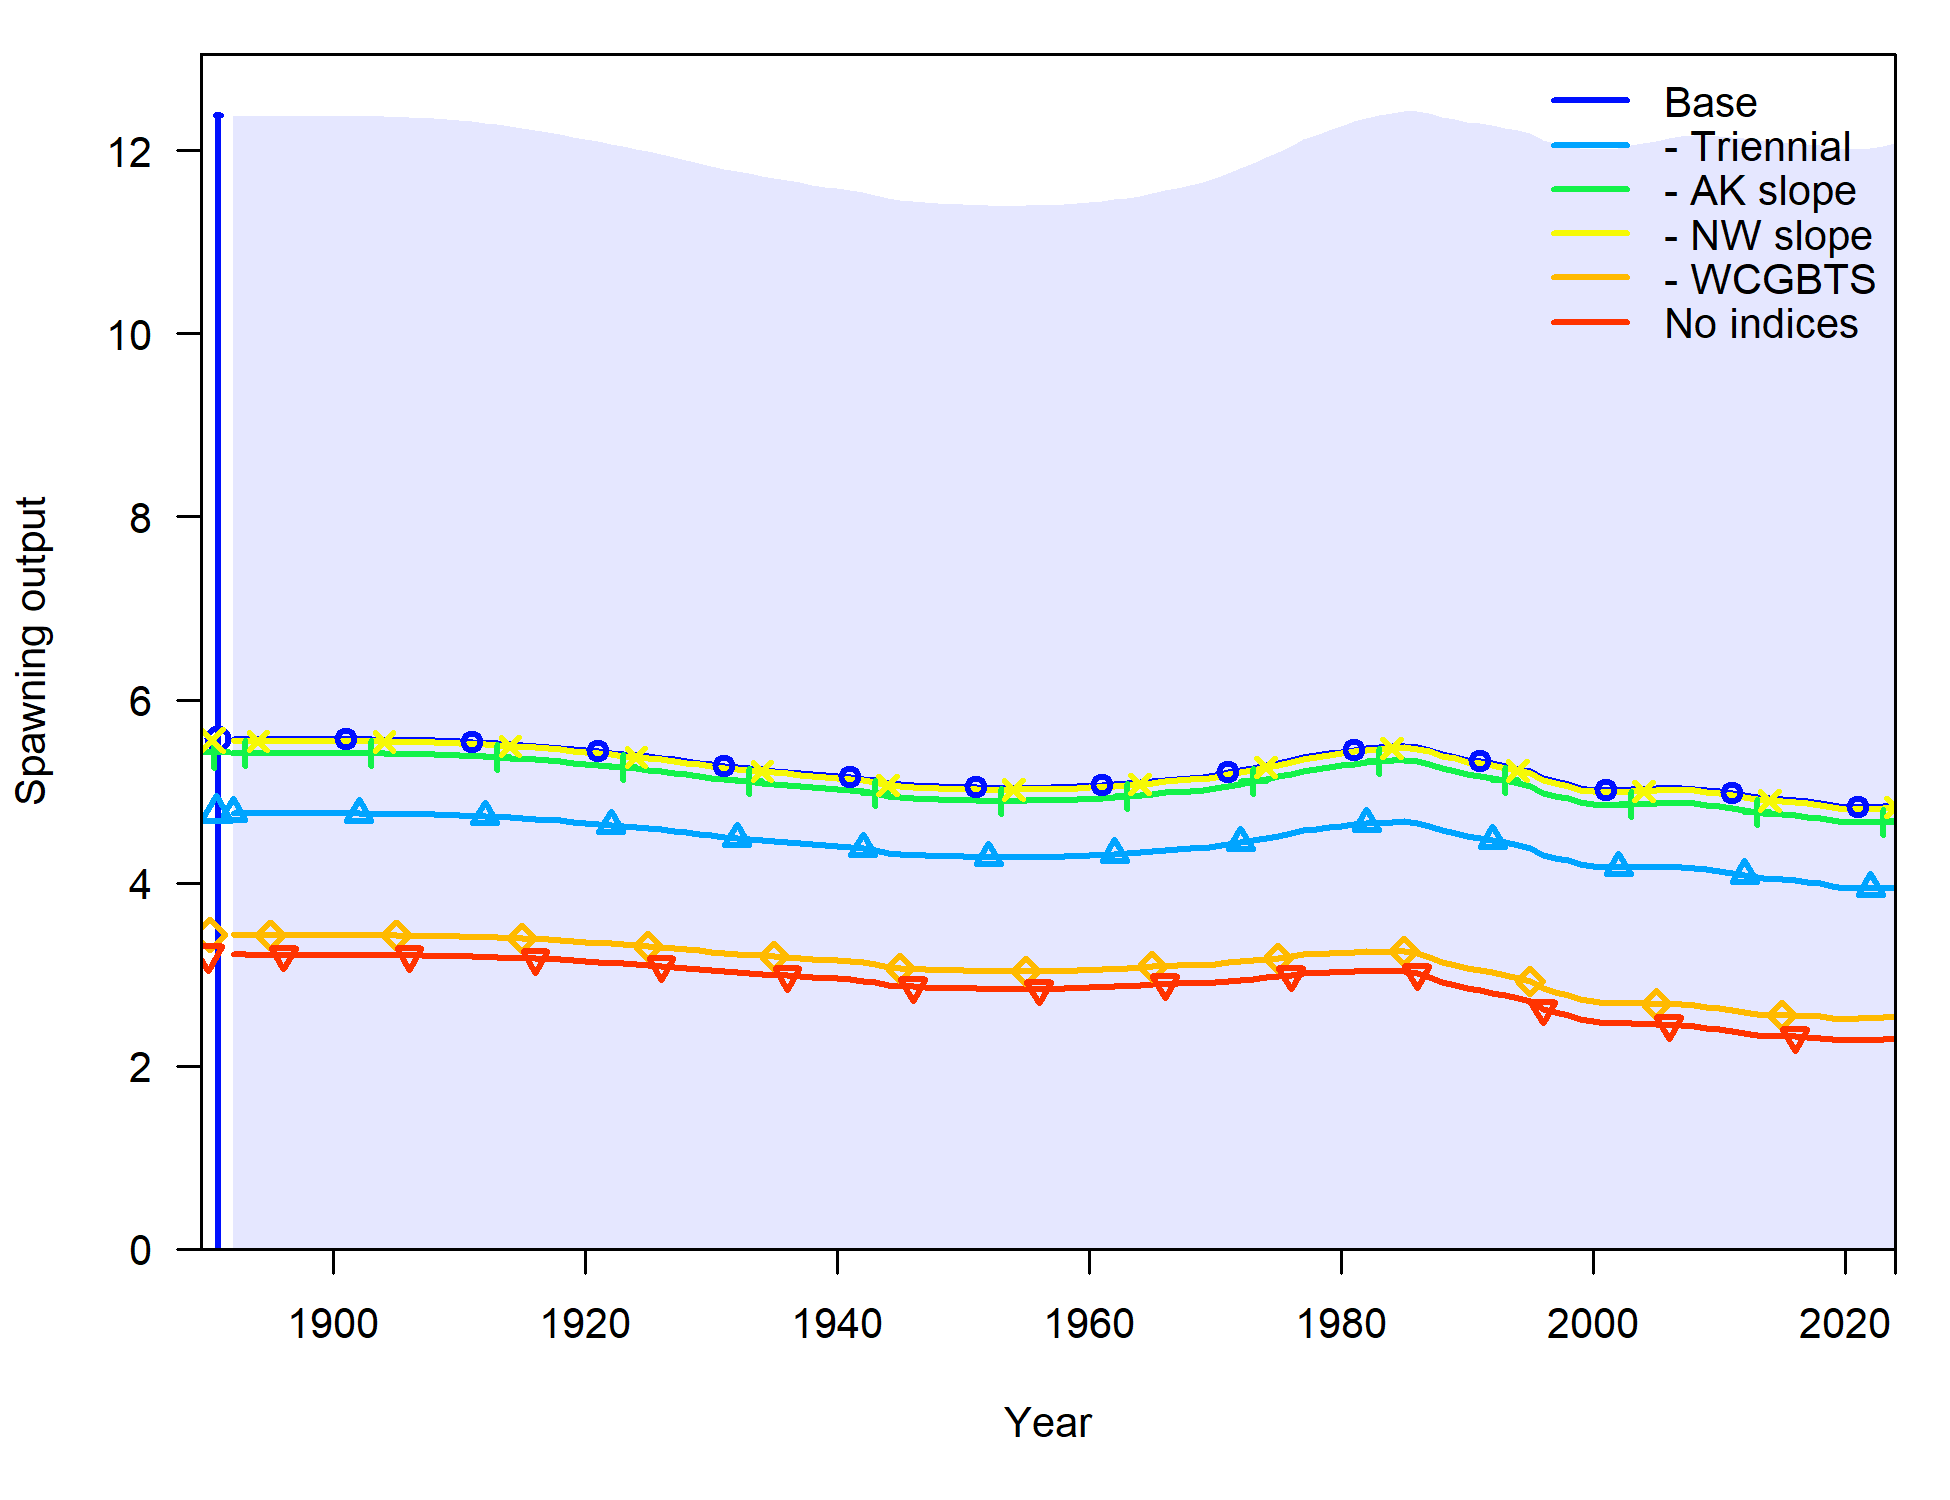
\includegraphics{Sensis/output/indicescompare2_spawnbio_uncertainty.png}

}

\caption{\label{fig-sens_indices_spout}Spawning output (trillions of
eggs) across data removal sensitivities (indices).}

\end{figure}%

\begin{figure}[H]

\centering{

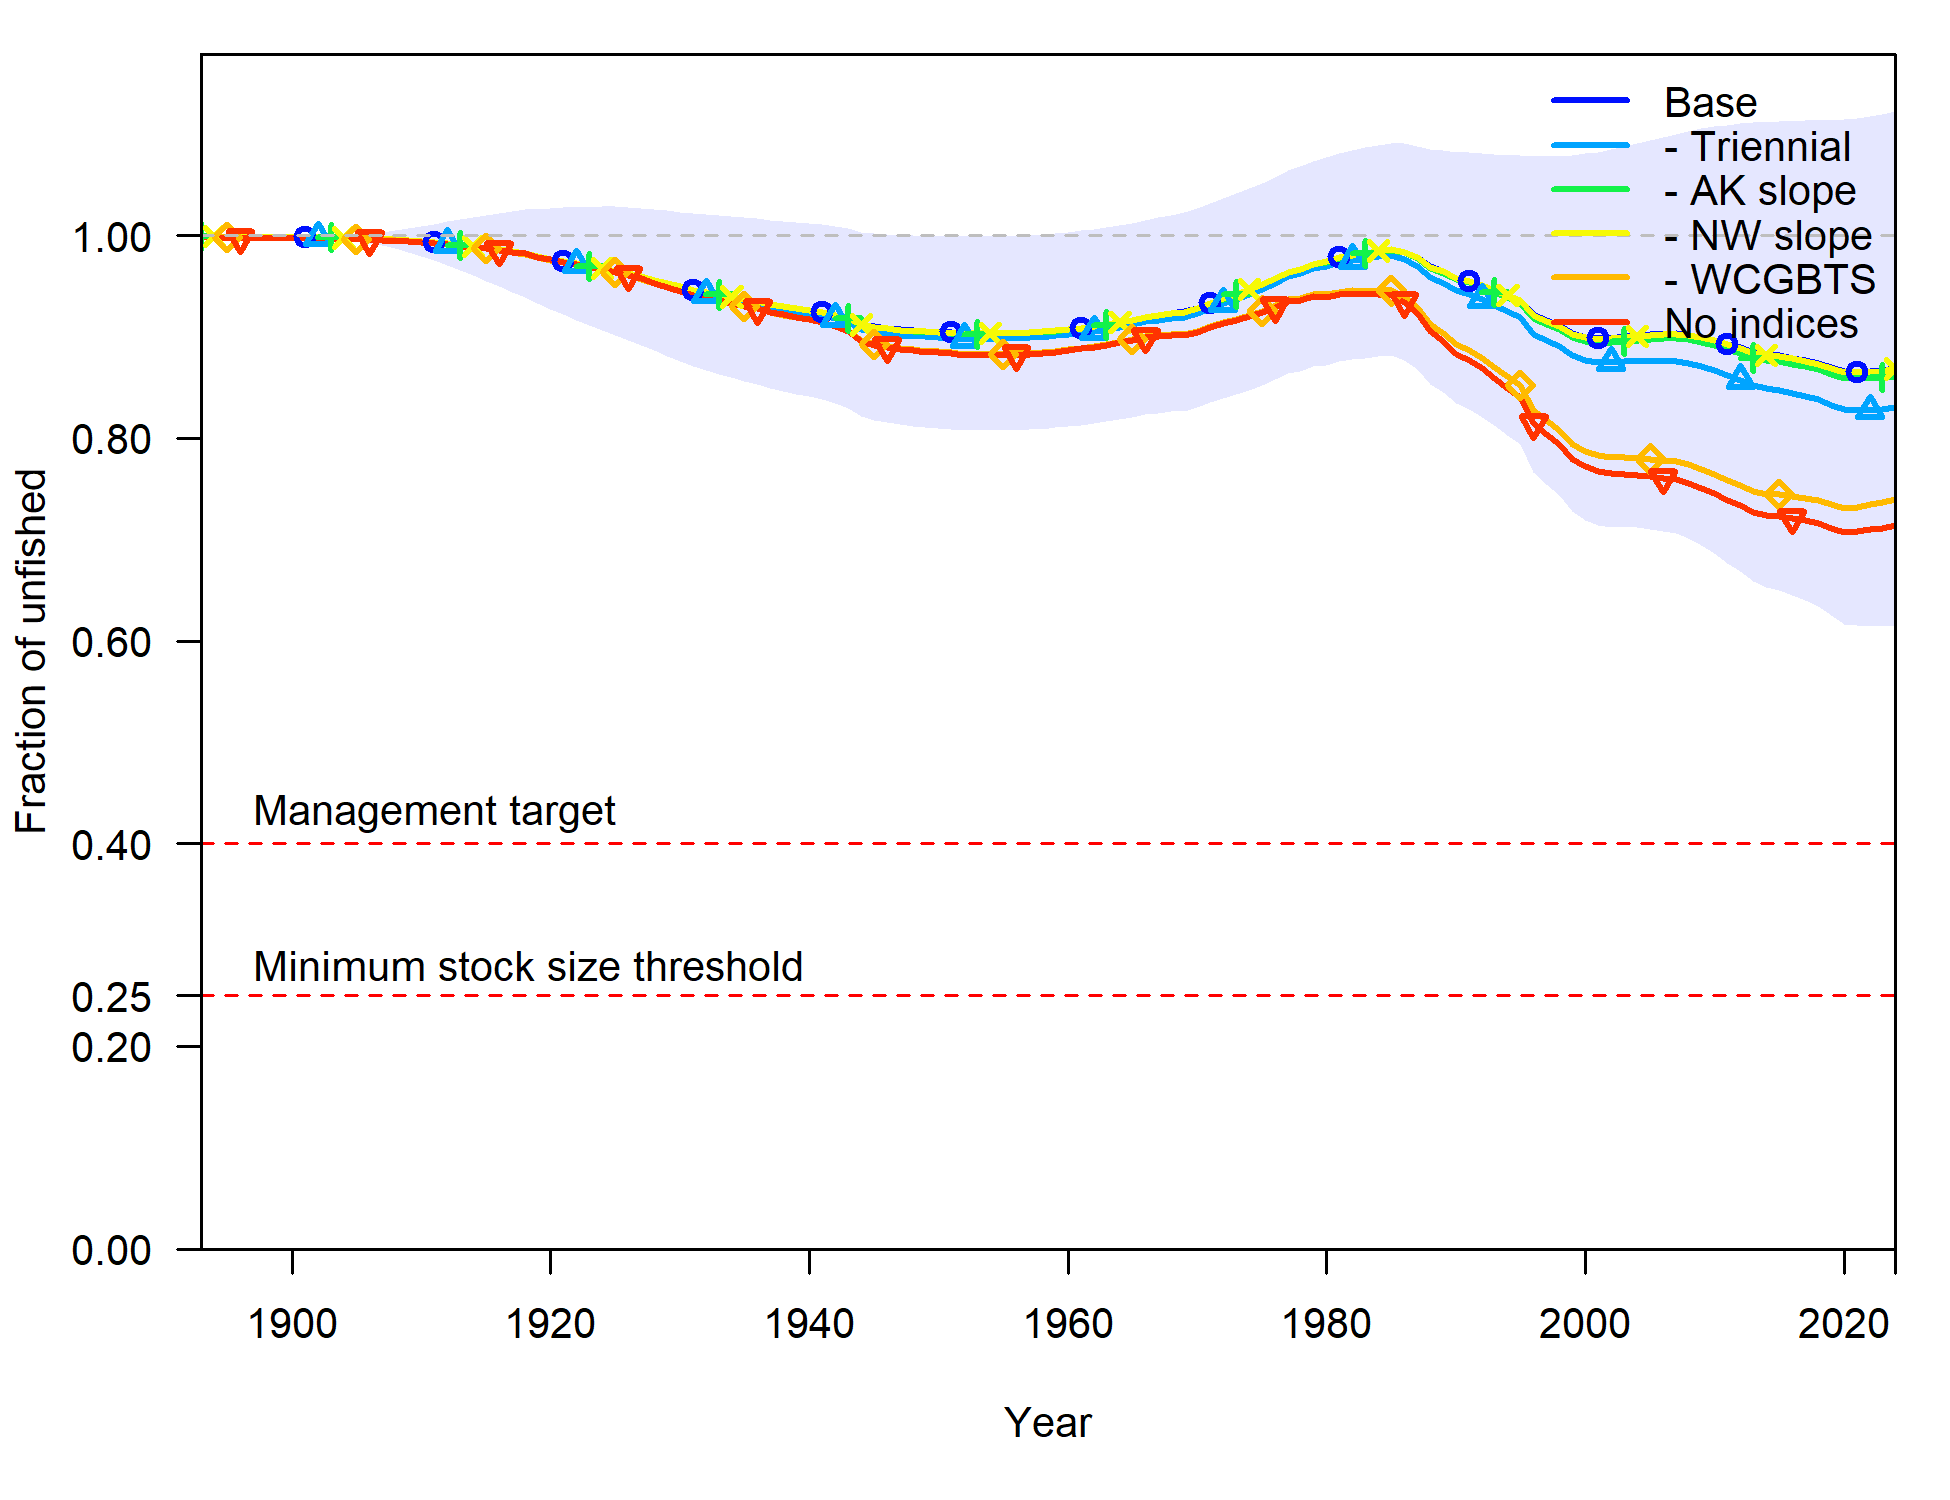
\includegraphics{Sensis/output/indicescompare4_Bratio_uncertainty.png}

}

\caption{\label{fig-sens_indices_relsp}Relative spawning output
(fraction unfished) across data removal sensitivities (indices).}

\end{figure}%

\begin{figure}[H]

\centering{

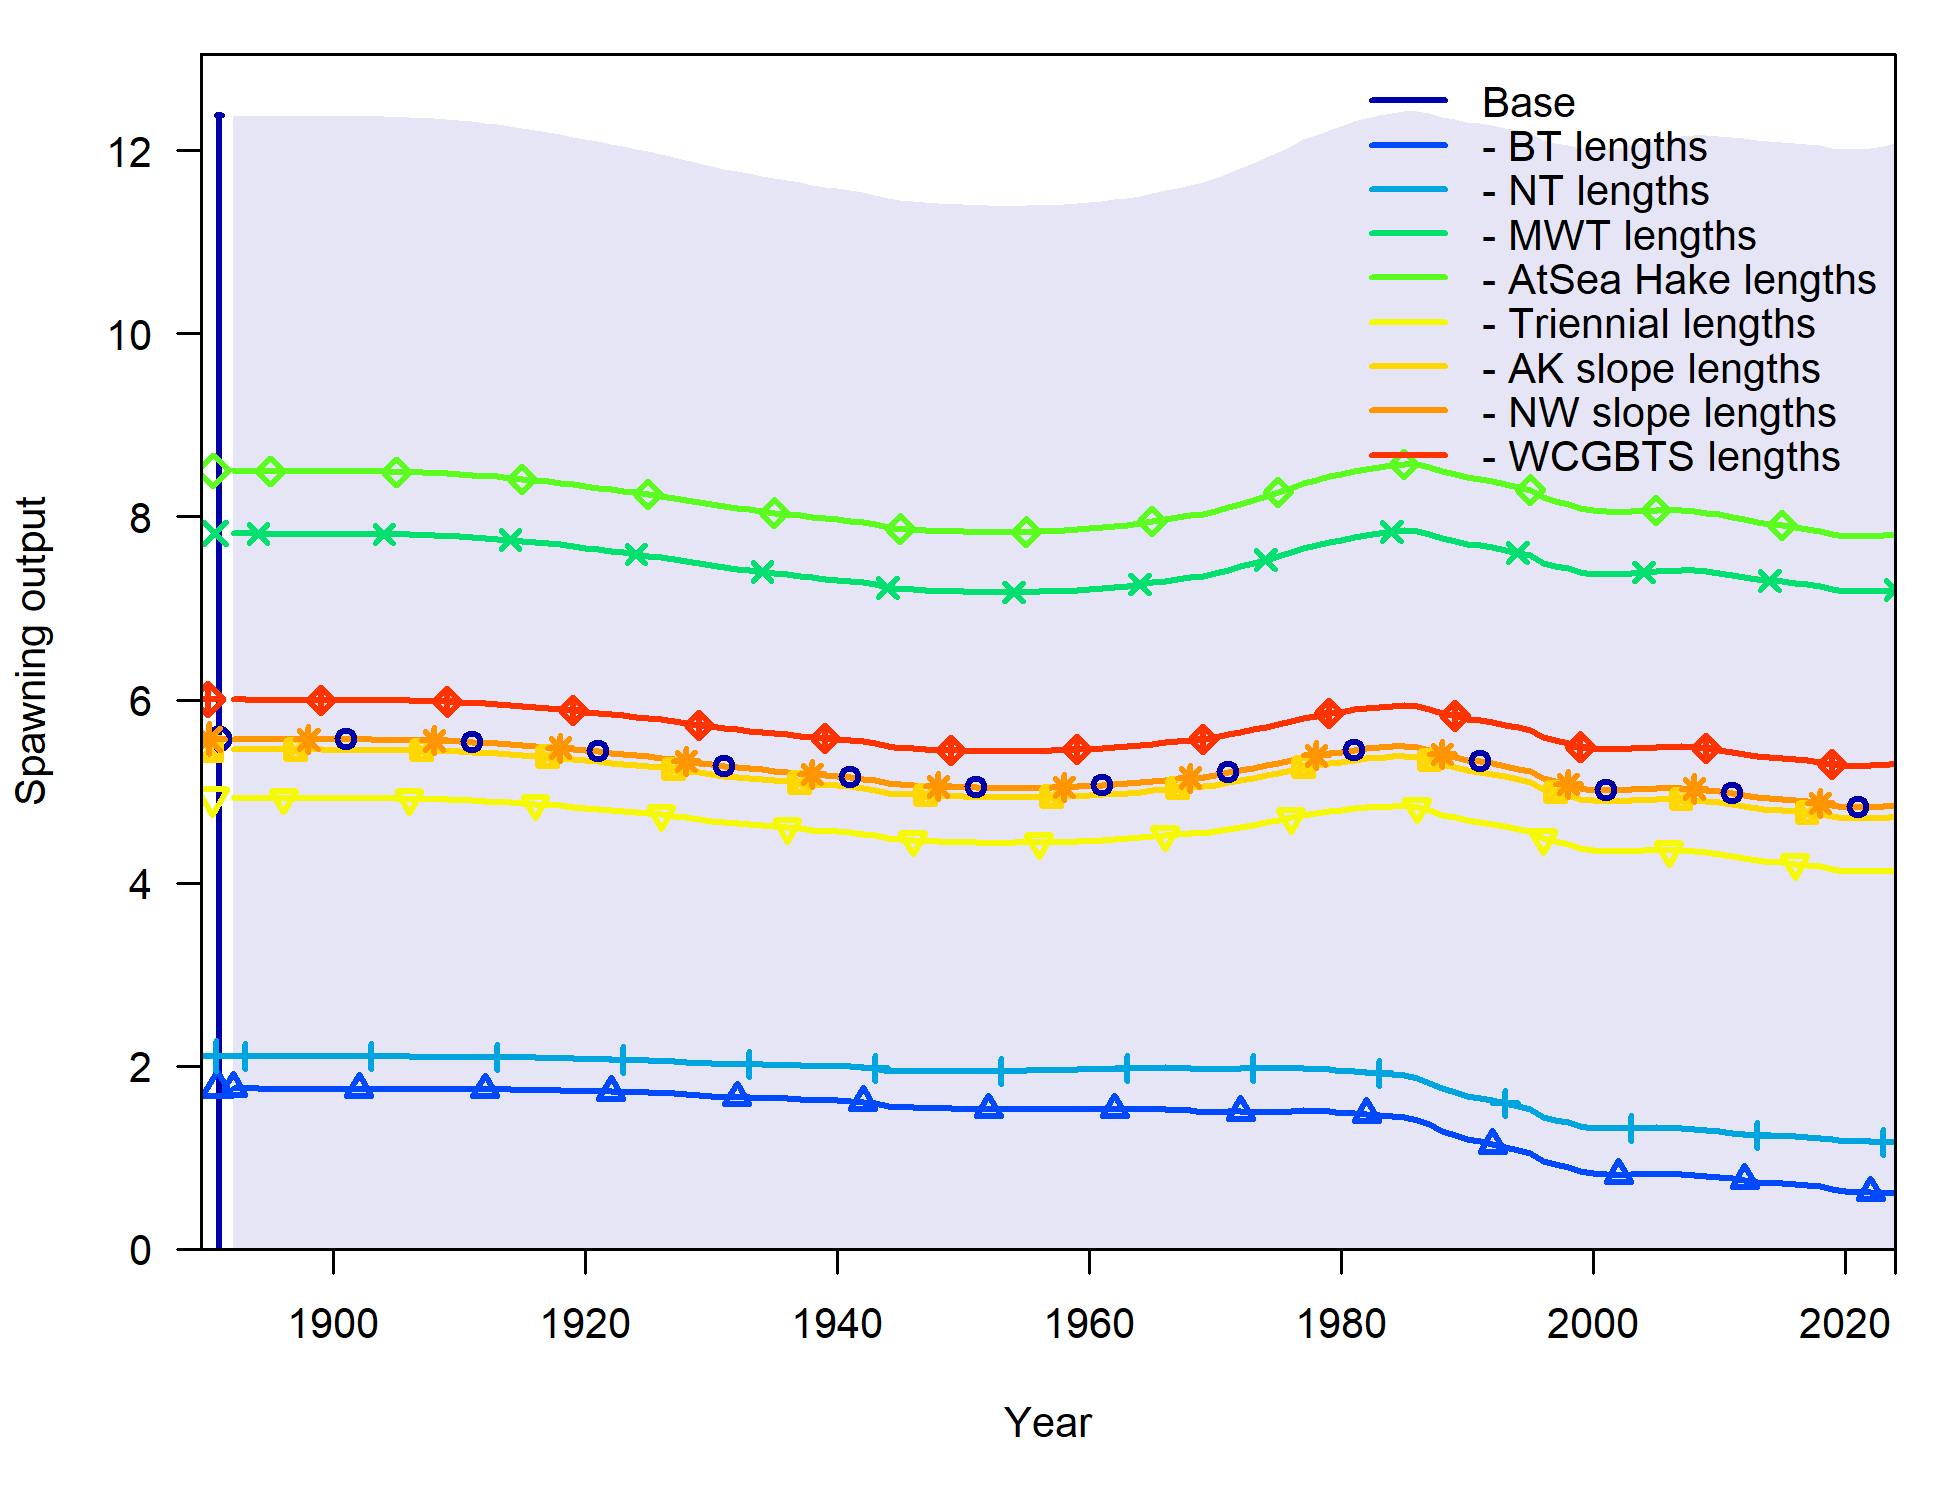
\includegraphics{Sensis/output/length_comps_fleetcompare2_spawnbio_uncertainty.png}

}

\caption{\label{fig-sens_lens1_spout}Spawning output (trillions of eggs)
across data removal sensitivities (length compositions by fleet).}

\end{figure}%

\begin{figure}[H]

\centering{

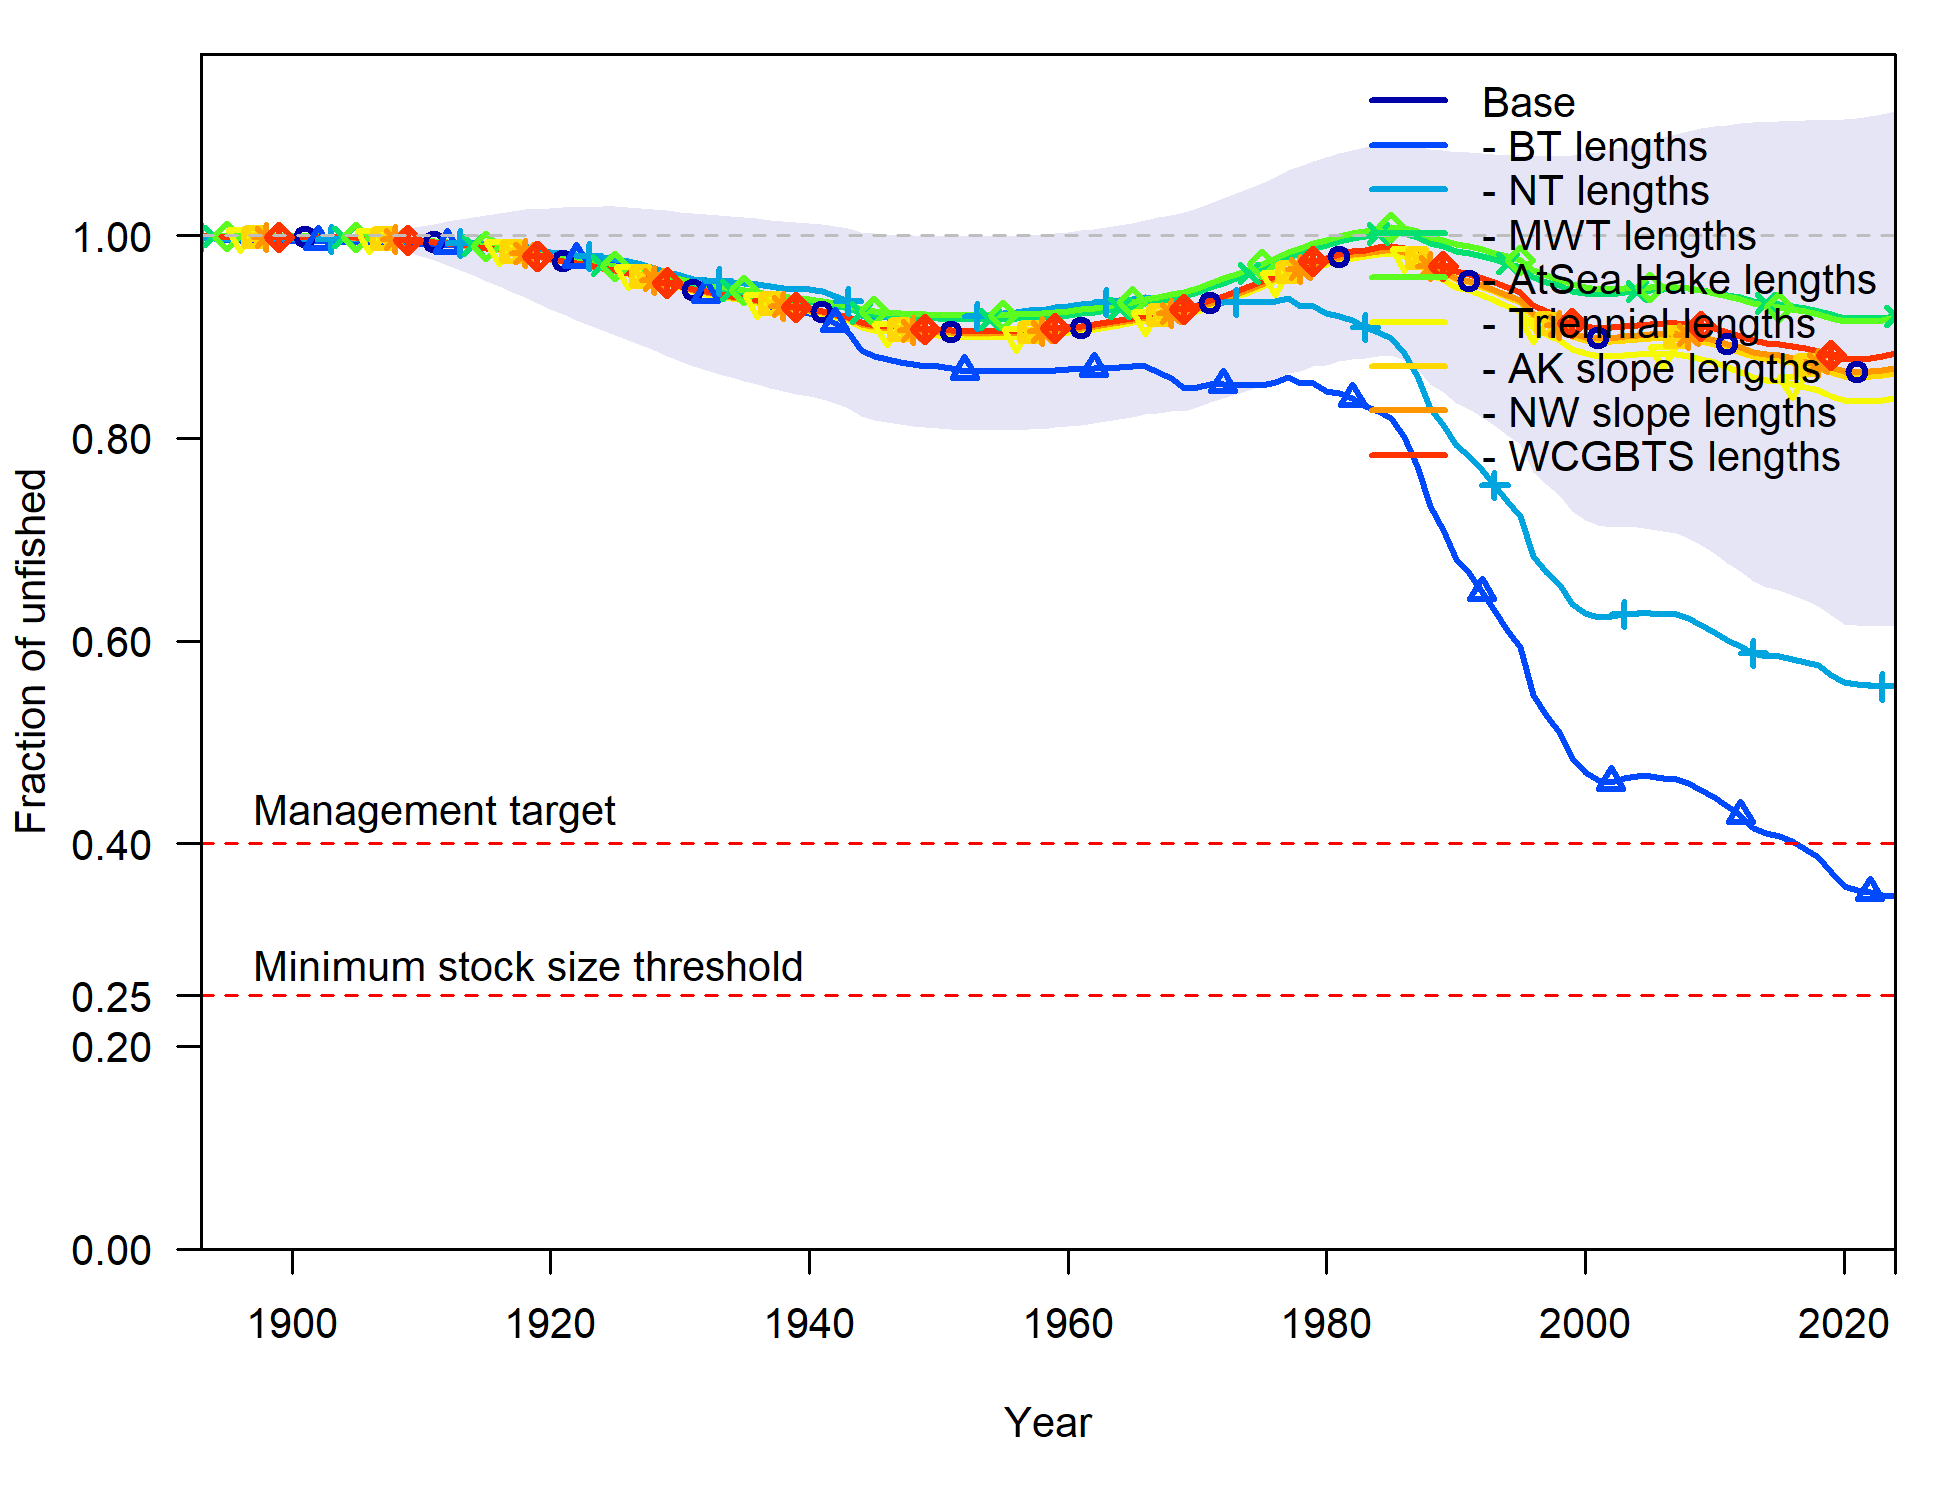
\includegraphics{Sensis/output/length_comps_fleetcompare4_Bratio_uncertainty.png}

}

\caption{\label{fig-sens_lens1_relsp}Relative spawning output (fraction
unfished) across data removal sensitivities (length compositions by
fleet).}

\end{figure}%

\begin{figure}[H]

\centering{

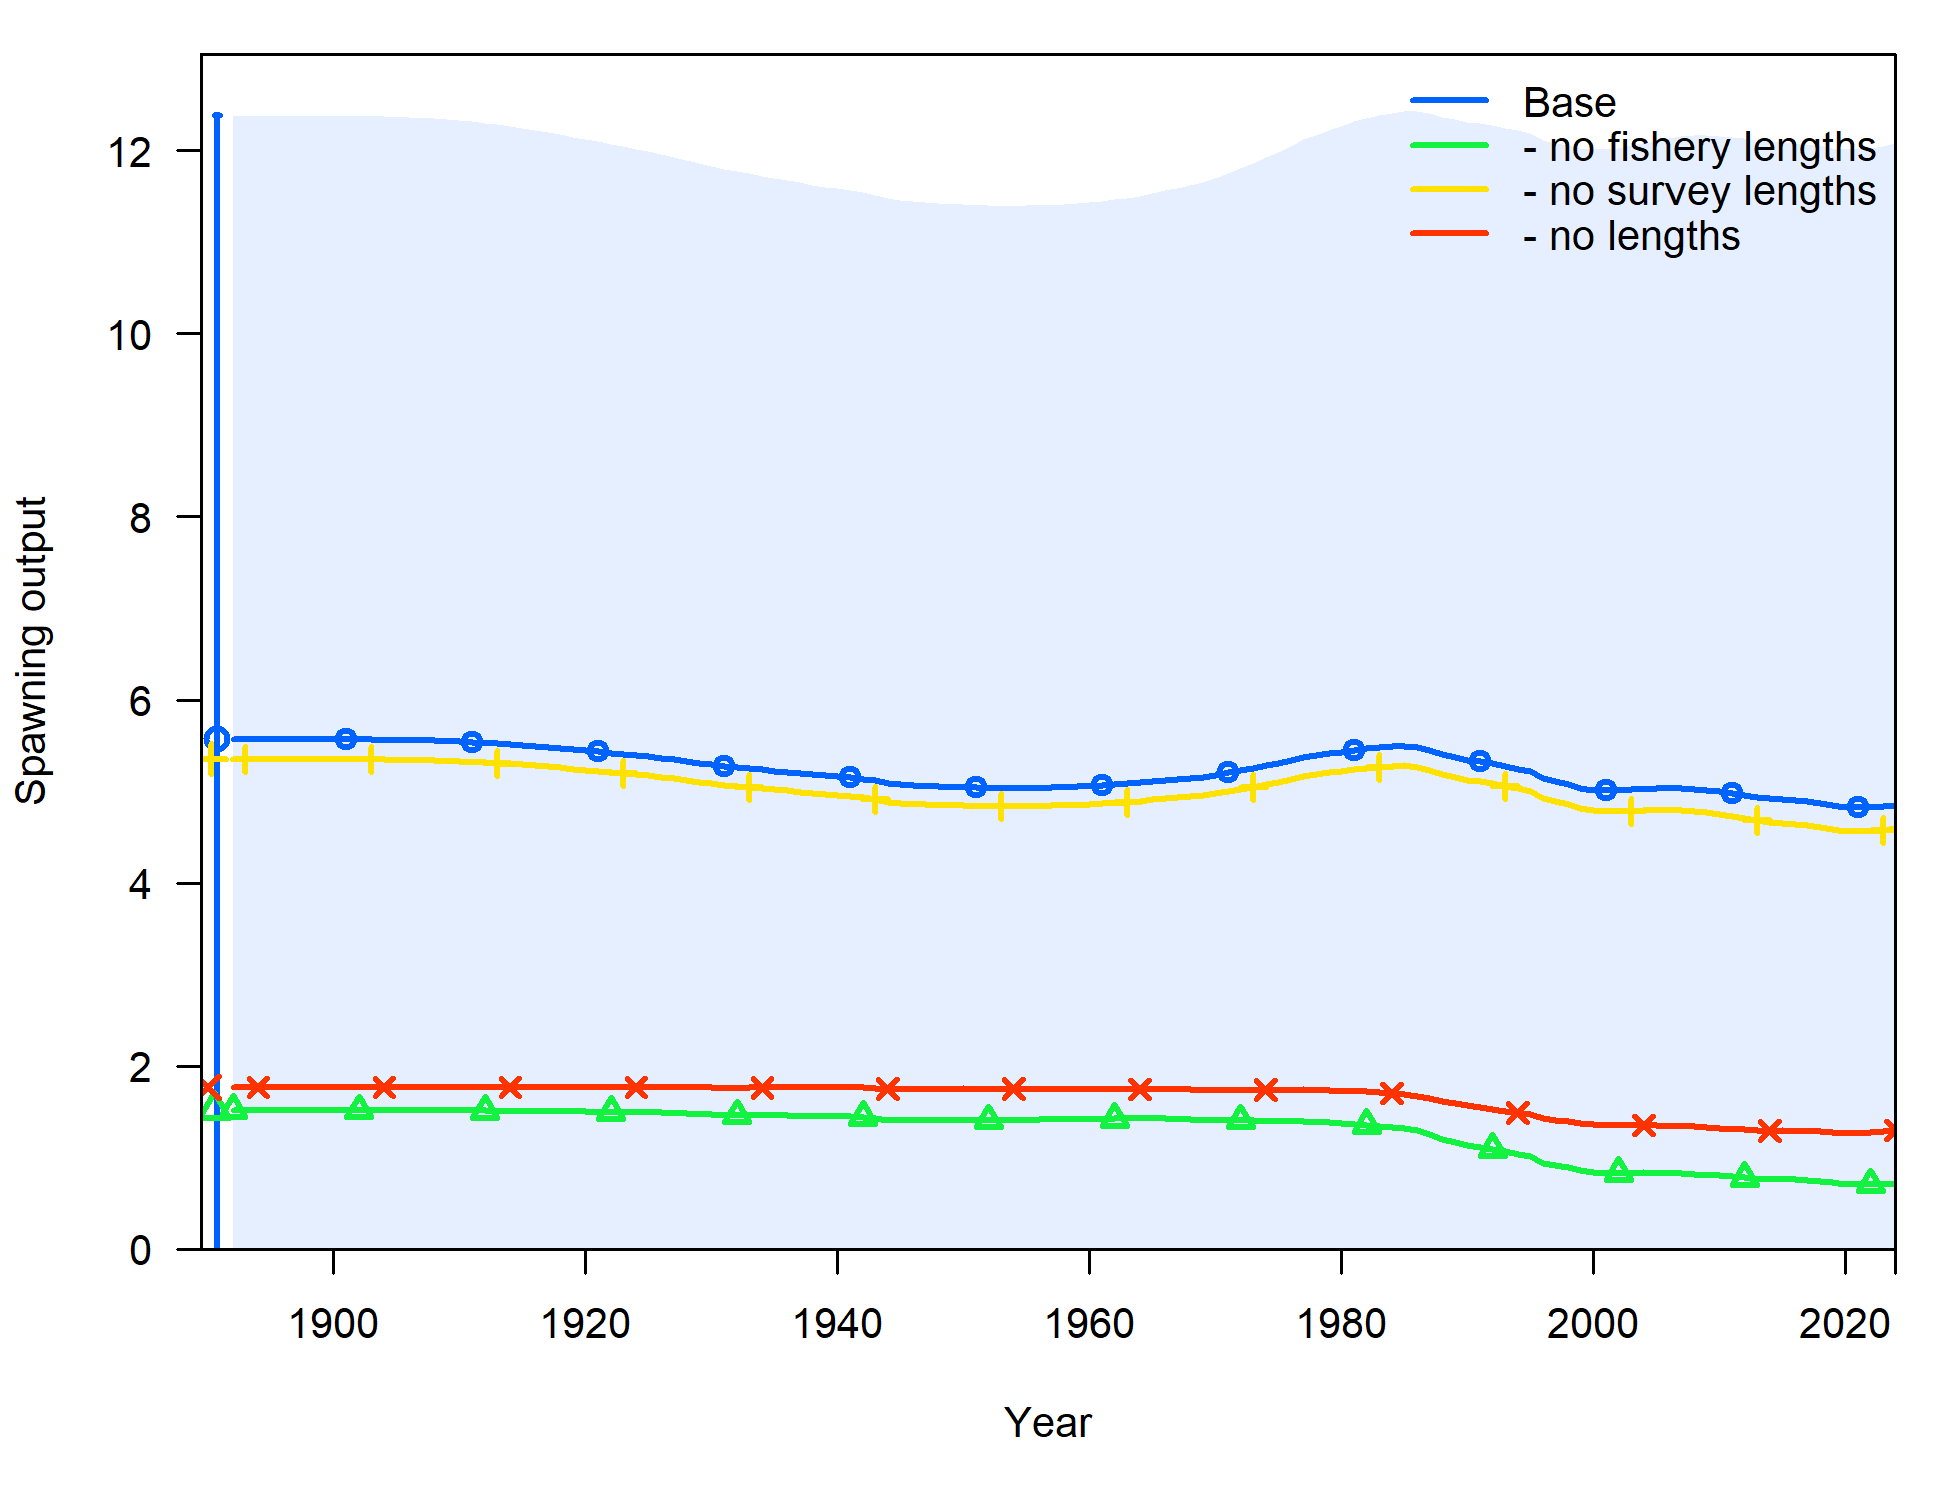
\includegraphics{Sensis/output/length_comps_allcompare2_spawnbio_uncertainty.png}

}

\caption{\label{fig-sens_lens2_spout}Spawning output (trillions of eggs)
across data removal sensitivities (length compositions by source).}

\end{figure}%

\begin{figure}[H]

\centering{

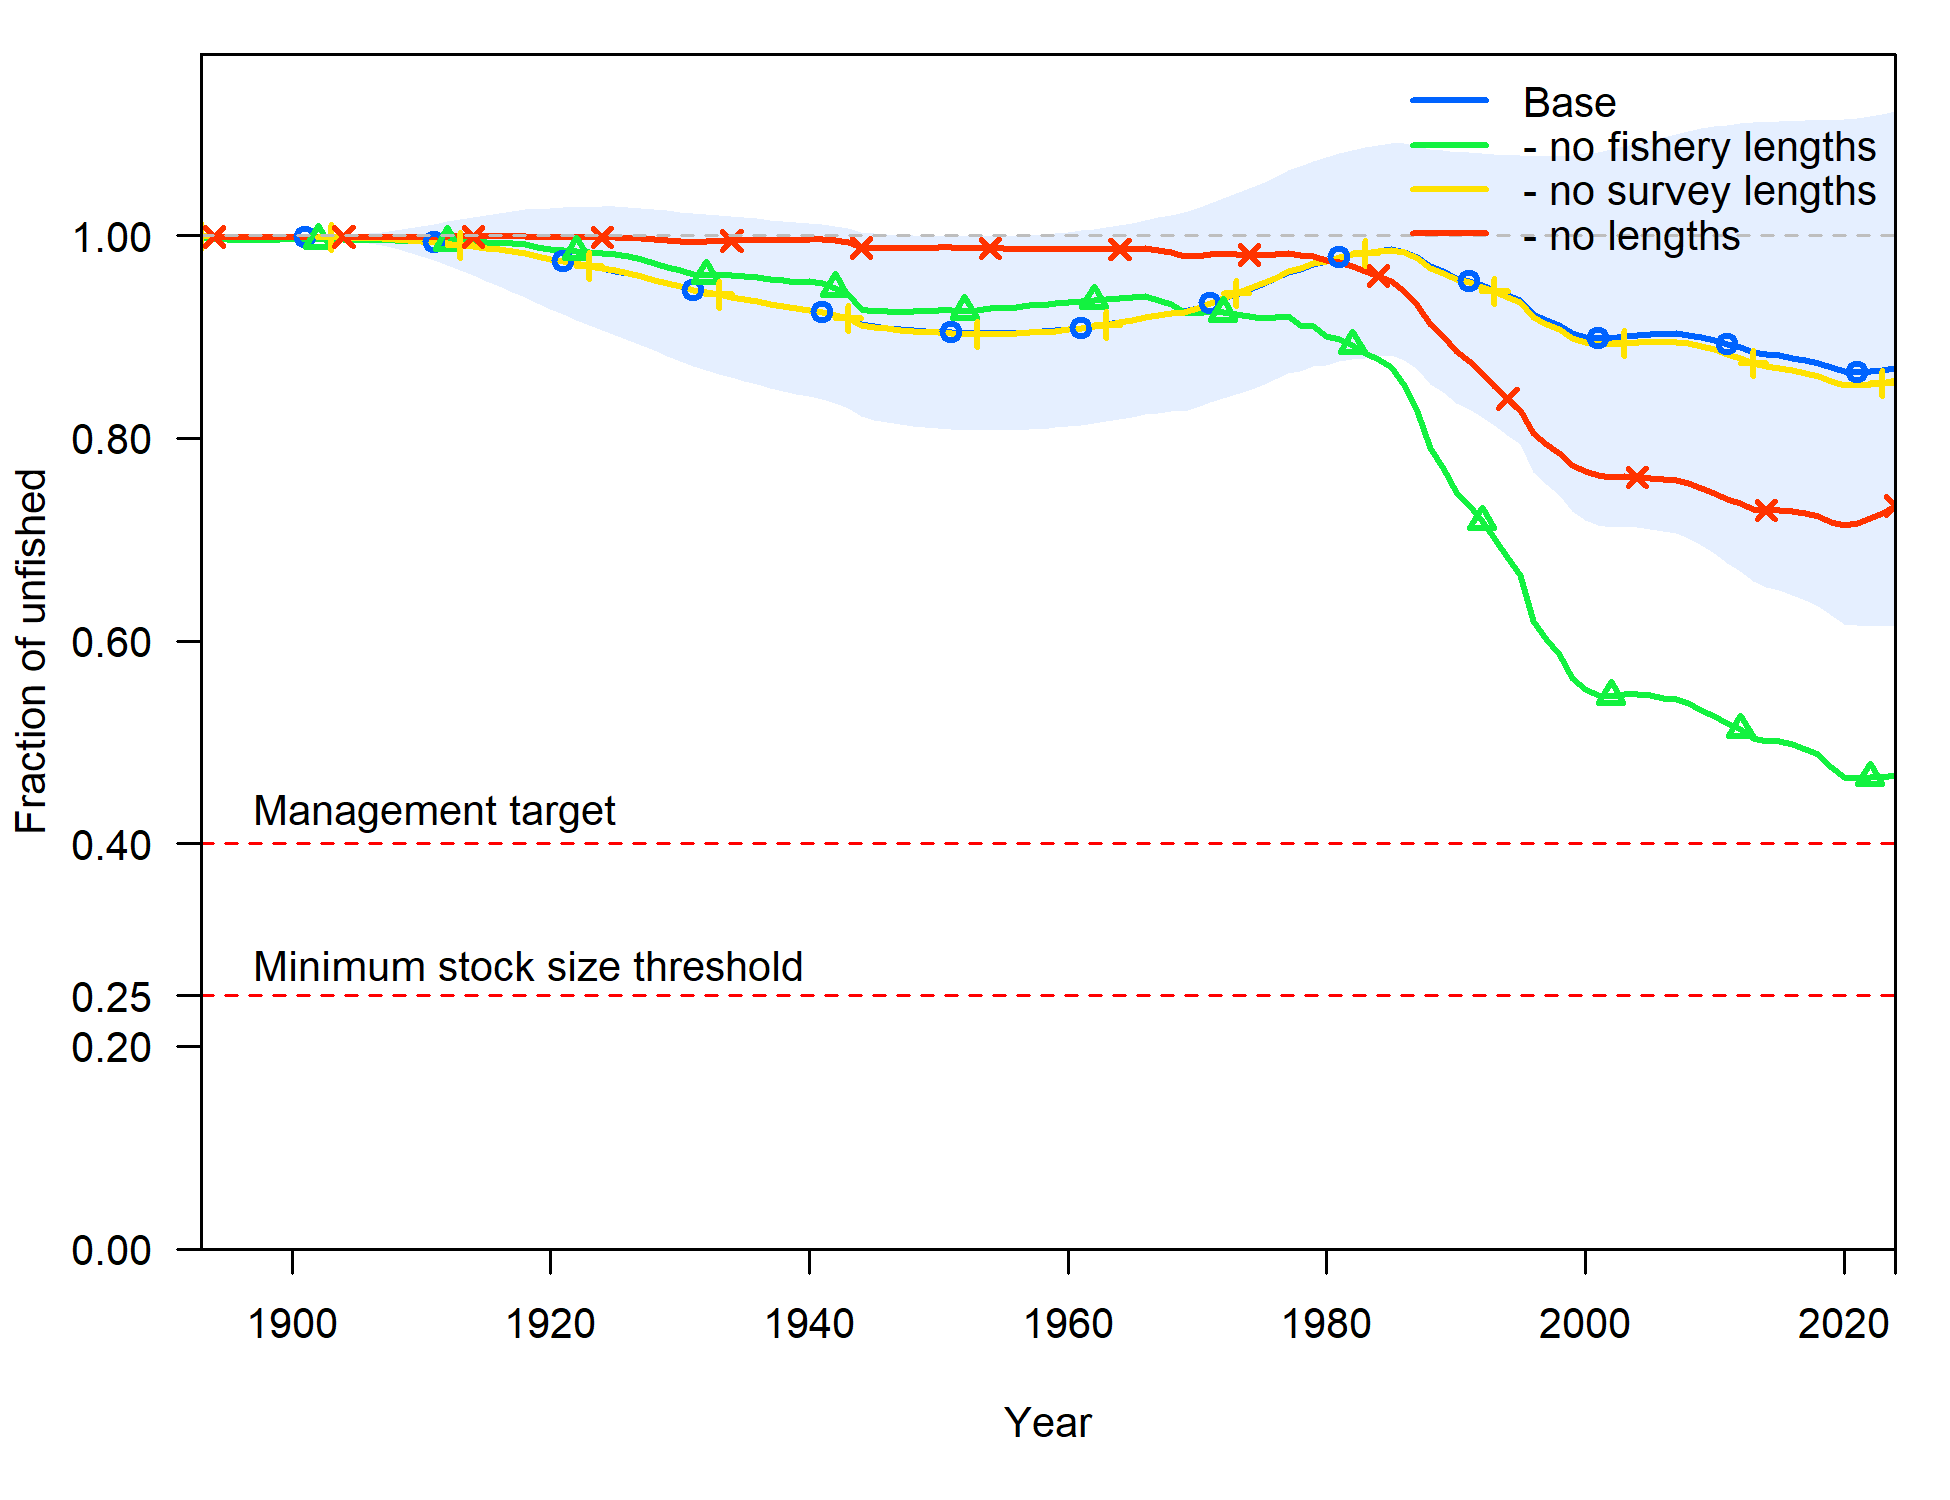
\includegraphics{Sensis/output/length_comps_allcompare4_Bratio_uncertainty.png}

}

\caption{\label{fig-sens_lens2_relsp}Relative spawning output (fraction
unfished) across data removal sensitivities (length compositions by
source).}

\end{figure}%

\begin{figure}[H]

\centering{

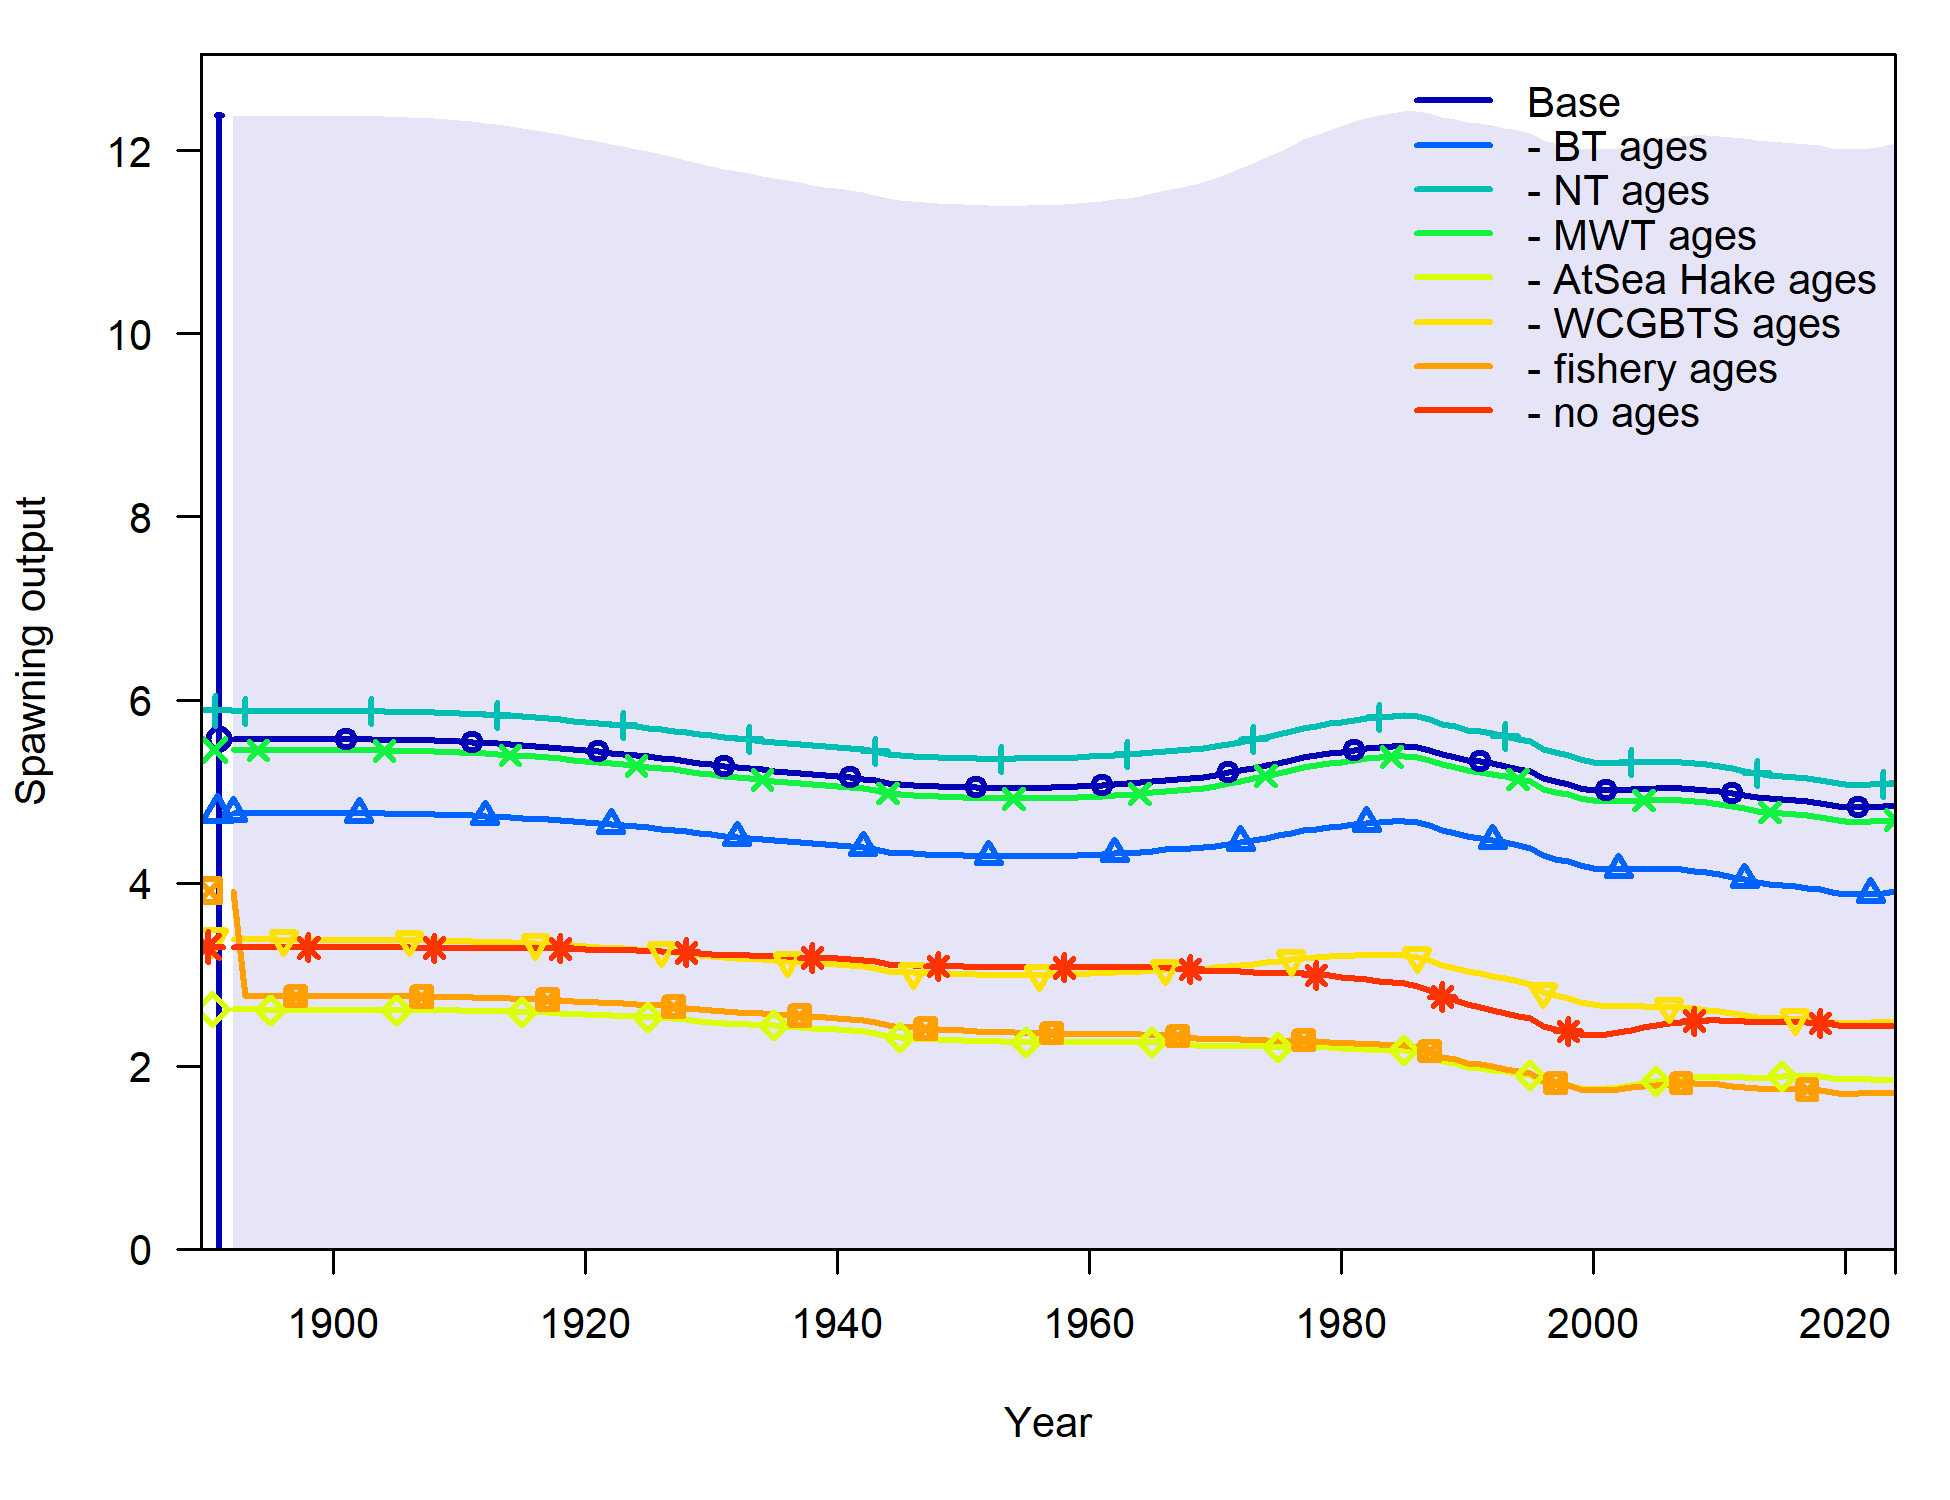
\includegraphics{Sensis/output/age_compscompare2_spawnbio_uncertainty.png}

}

\caption{\label{fig-sens_age_spout}Spawning output (trillions of eggs)
across data removal sensitivities (age compositions by fleet).}

\end{figure}%

\begin{figure}[H]

\centering{

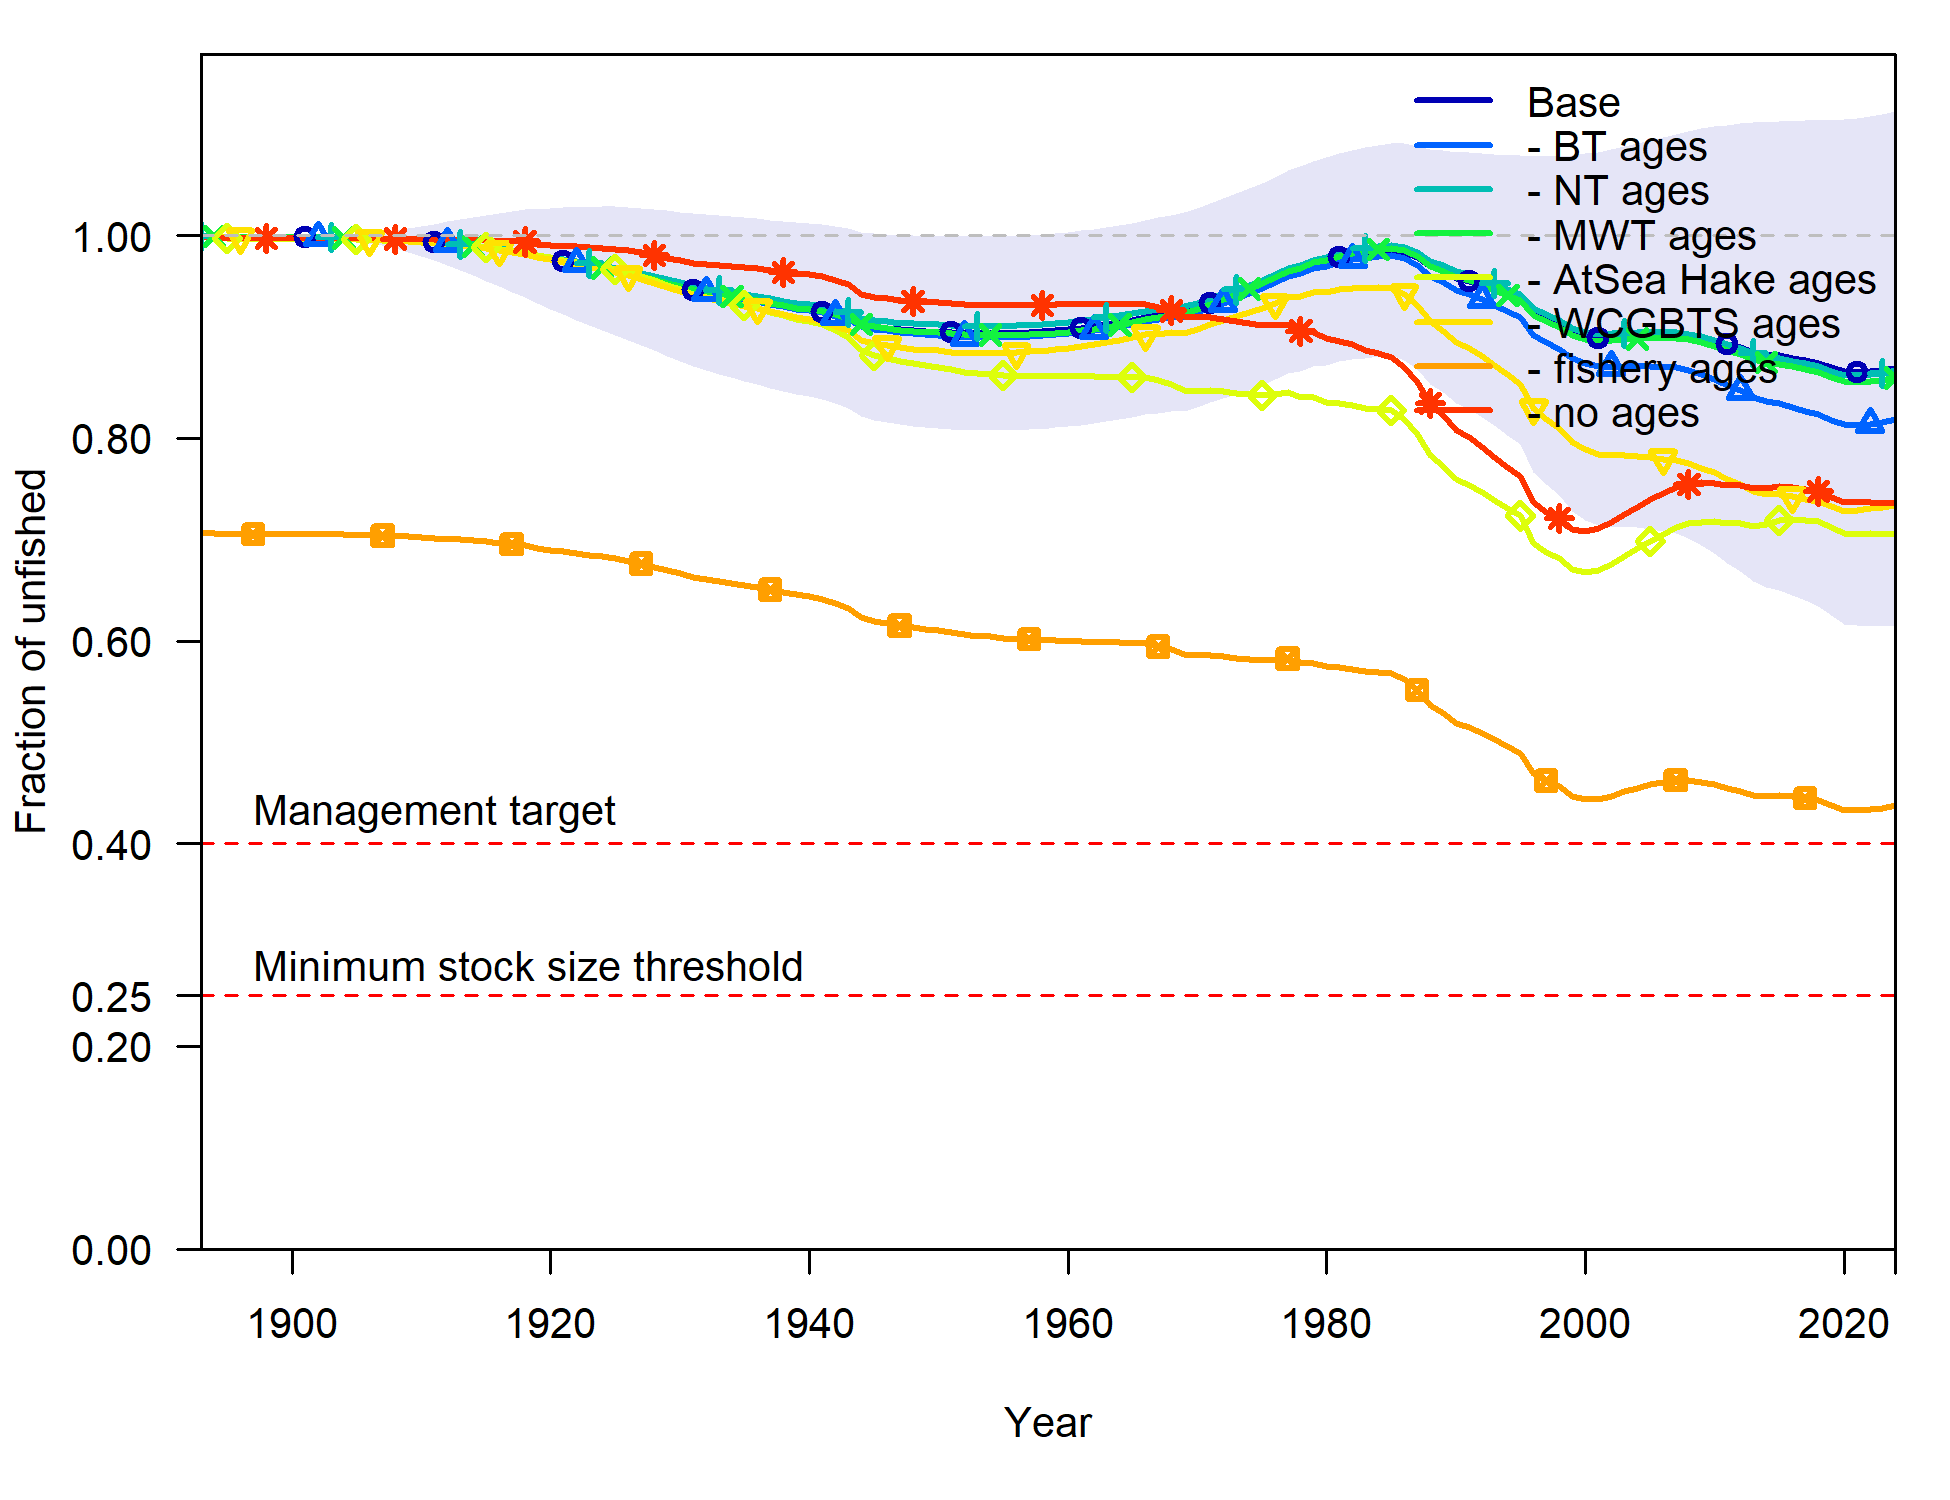
\includegraphics{Sensis/output/age_compscompare4_Bratio_uncertainty.png}

}

\caption{\label{fig-sens_age_relsp}Relative spawning output (fraction
unfished) across data removal sensitivities (age compositions by
fleet).}

\end{figure}%

\begin{figure}[H]

\centering{

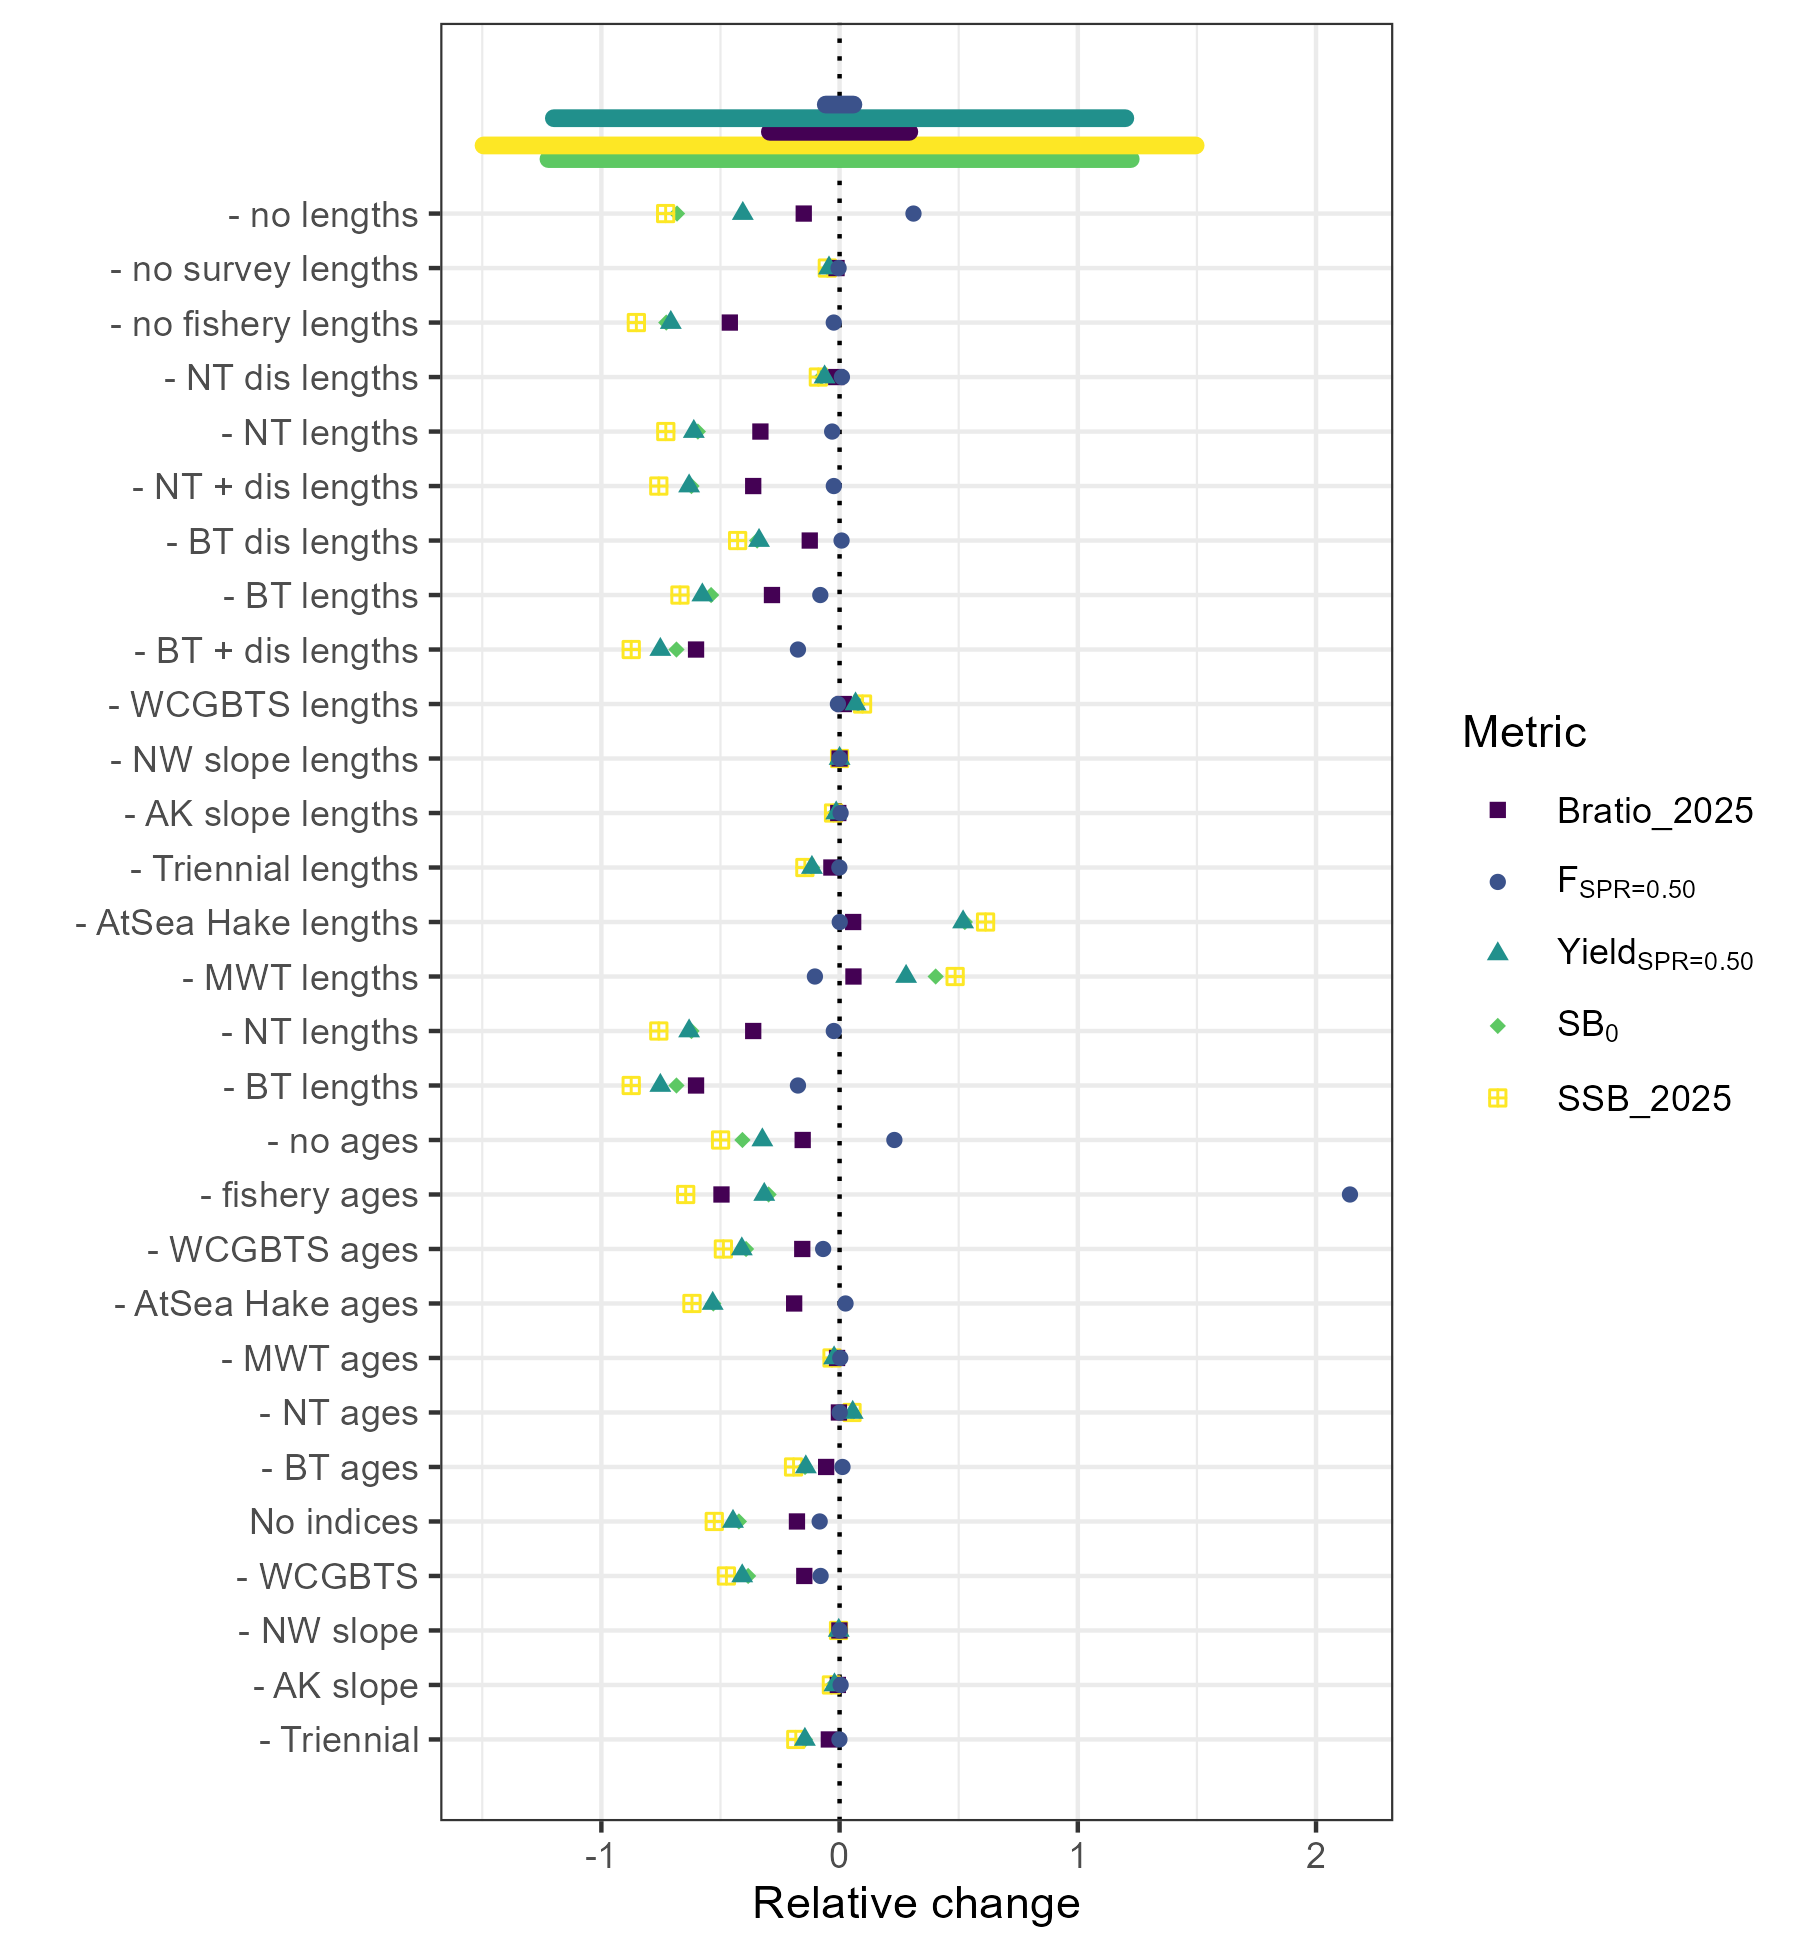
\includegraphics{Sensis/output/sens_summary.png}

}

\caption{\label{fig-sens_sum_data}Relative change in management
quantities across models conducted as sensitivities (removal of data
sources).}

\end{figure}%

\begin{figure}[H]

\centering{

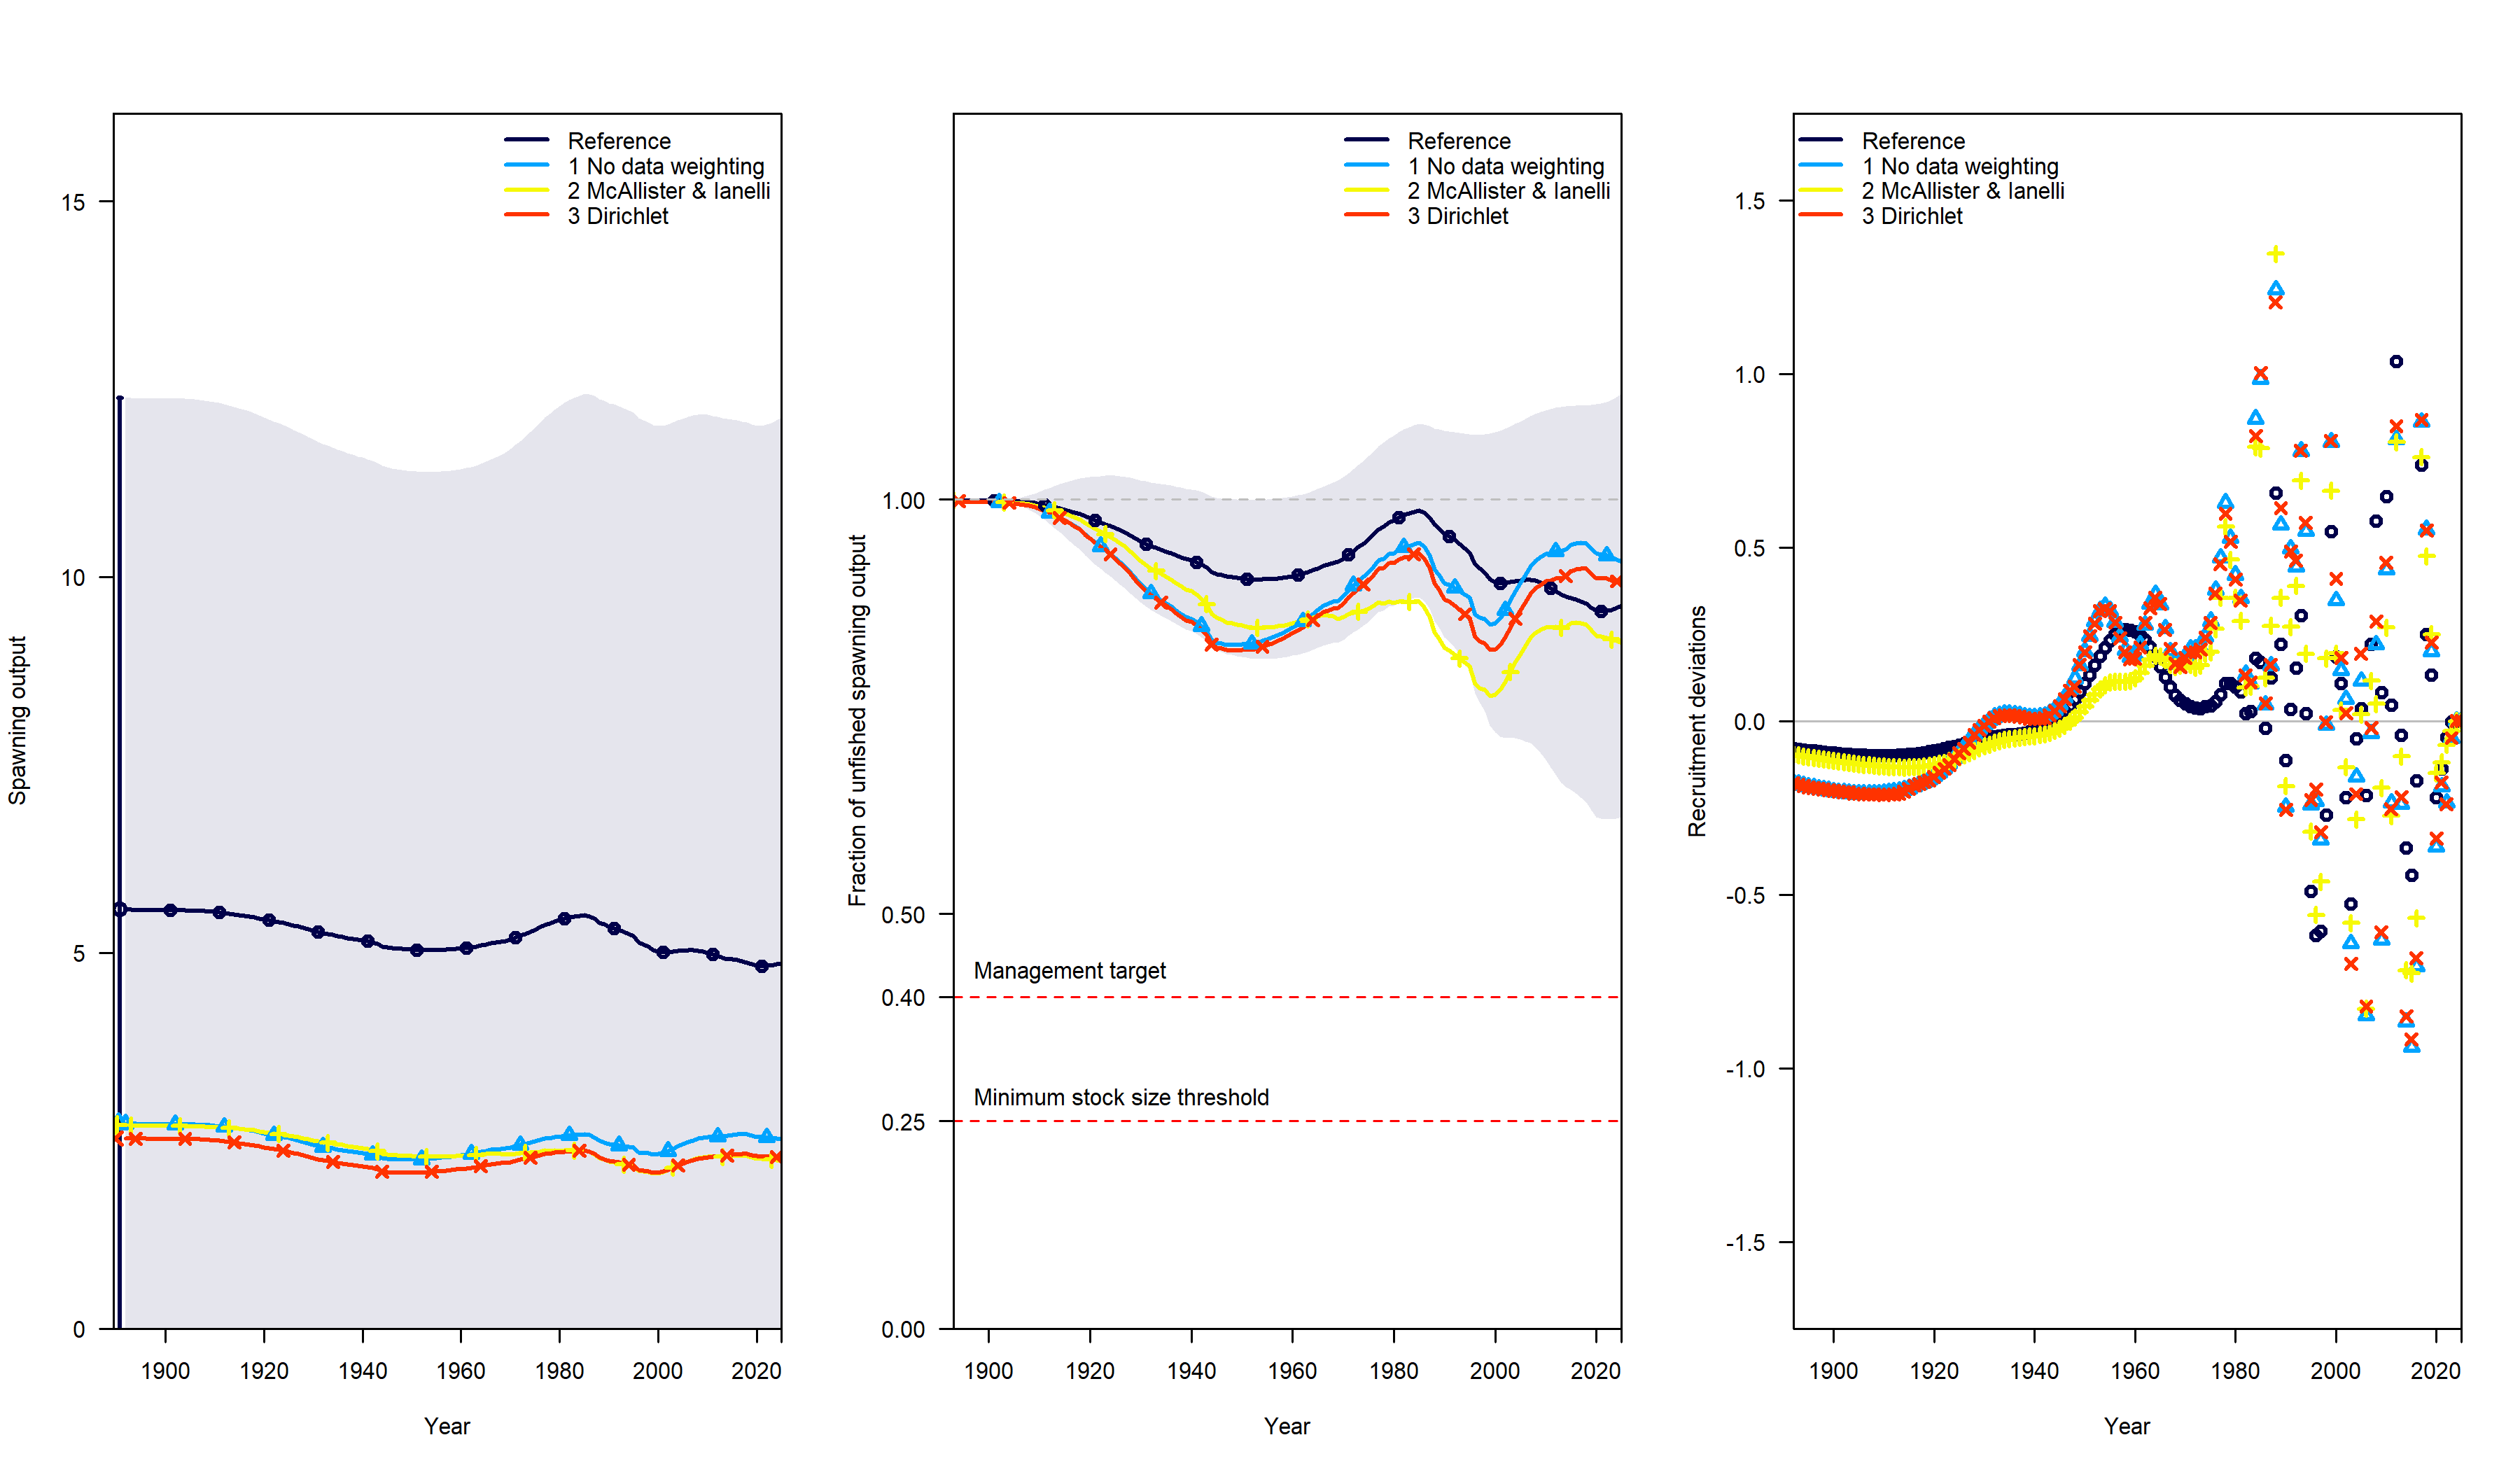
\includegraphics{Sensis/data_sensitivities/Data weighting.png}

}

\caption{\label{fig-sensi-data-wt}Comparison of spawning output
(trillions of eggs; left panel), relative stock status (middle panel)
and recruitment estimation (right panel) for models under different data
weighting scenarios. The reference model uses the Francis method.}

\end{figure}%

\begin{figure}[H]

\centering{

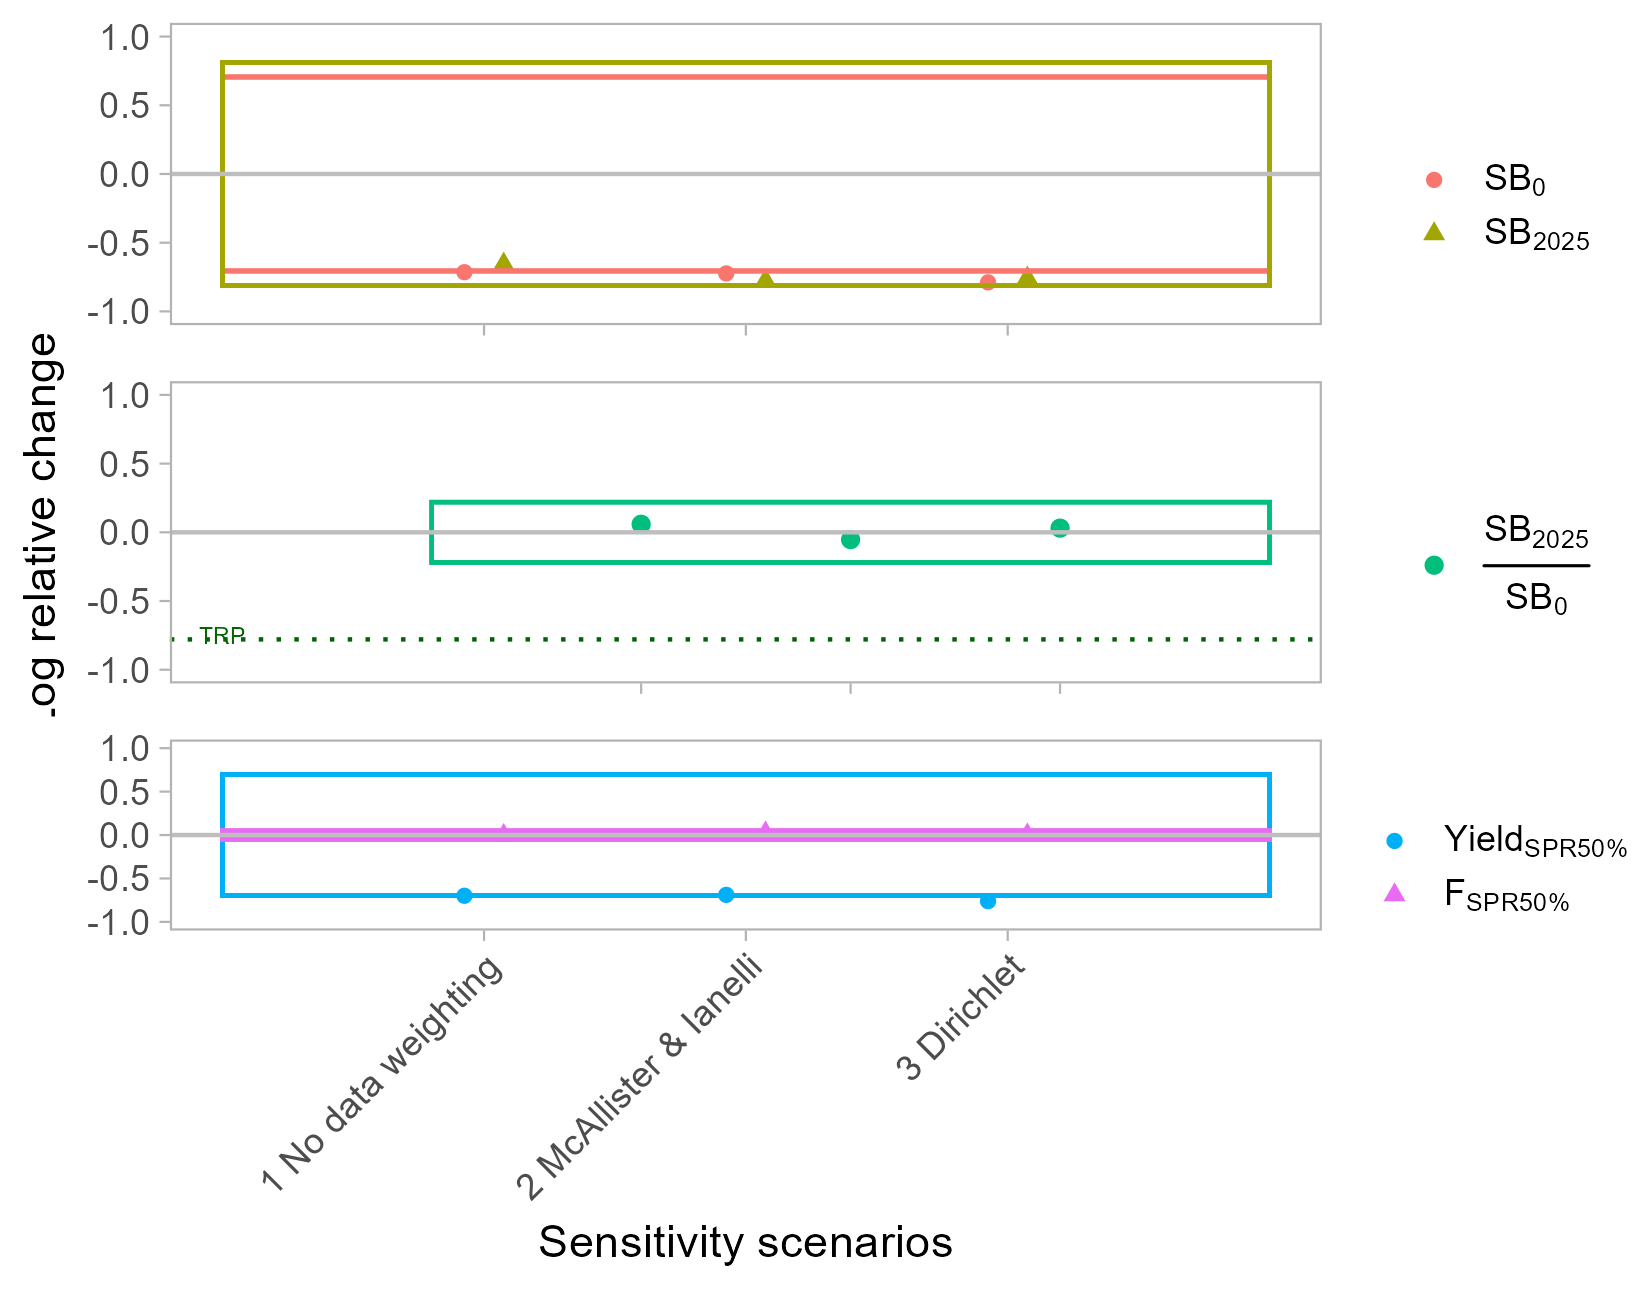
\includegraphics{Sensis/data_sensitivities/Sensi_logREplot_SB_Dep_F_Yield_DataWt.png}

}

\caption{\label{fig-sensi-RE-data-wt}Log relative change
(log((Model\_sensi-Model\_ref)/Model\_ref)) in data weighting treatment
for 5 derived quantities. Colored boxes indicate 95 percent confidence
interval of the reference model. See `Sensitivity Analysis' section for
more details on each scenario.}

\end{figure}%

\begin{figure}[H]

\centering{

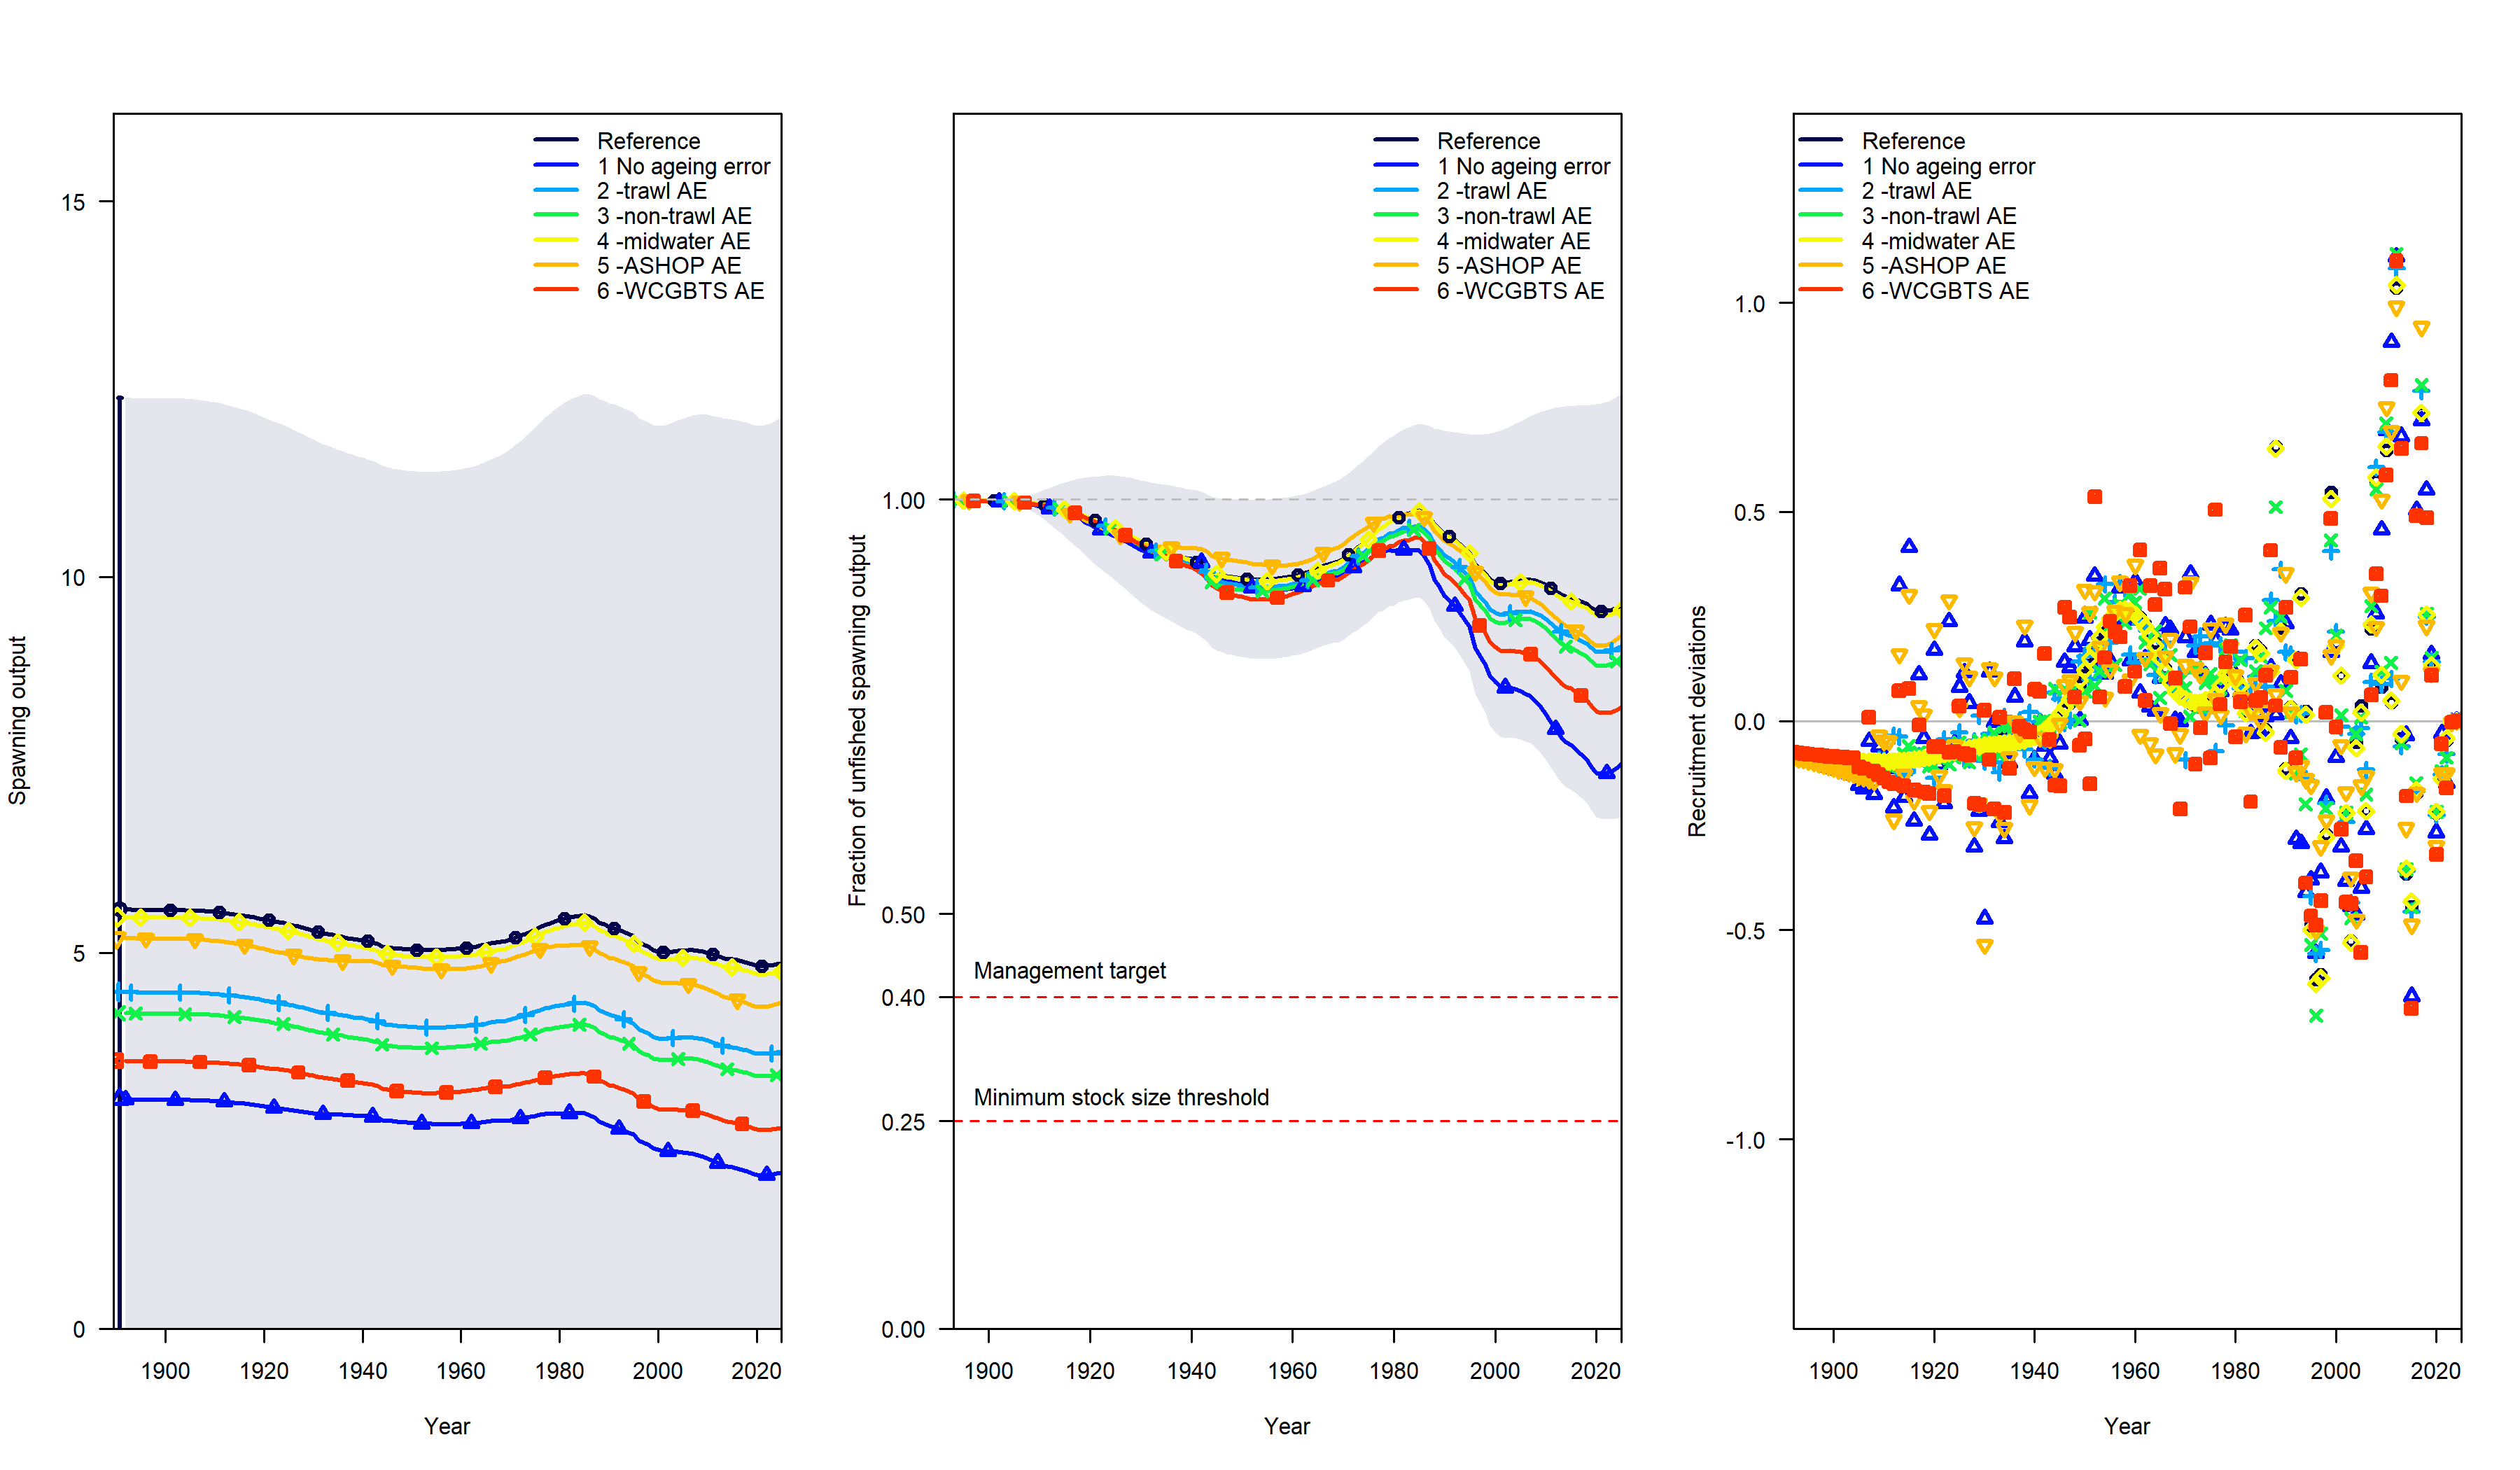
\includegraphics{Sensis/data_sensitivities/Ageing error_uncertainty.png}

}

\caption{\label{fig-sensi-ageing-error}Comparison of spawning output
(trillions of eggs; left panel), relative stock status (middle panel)
and recruitment estimation (right panel) for models under different
ageing error scenarios. The reference model uses ageing error matrices
for all age sources.}

\end{figure}%

\begin{figure}[H]

\centering{

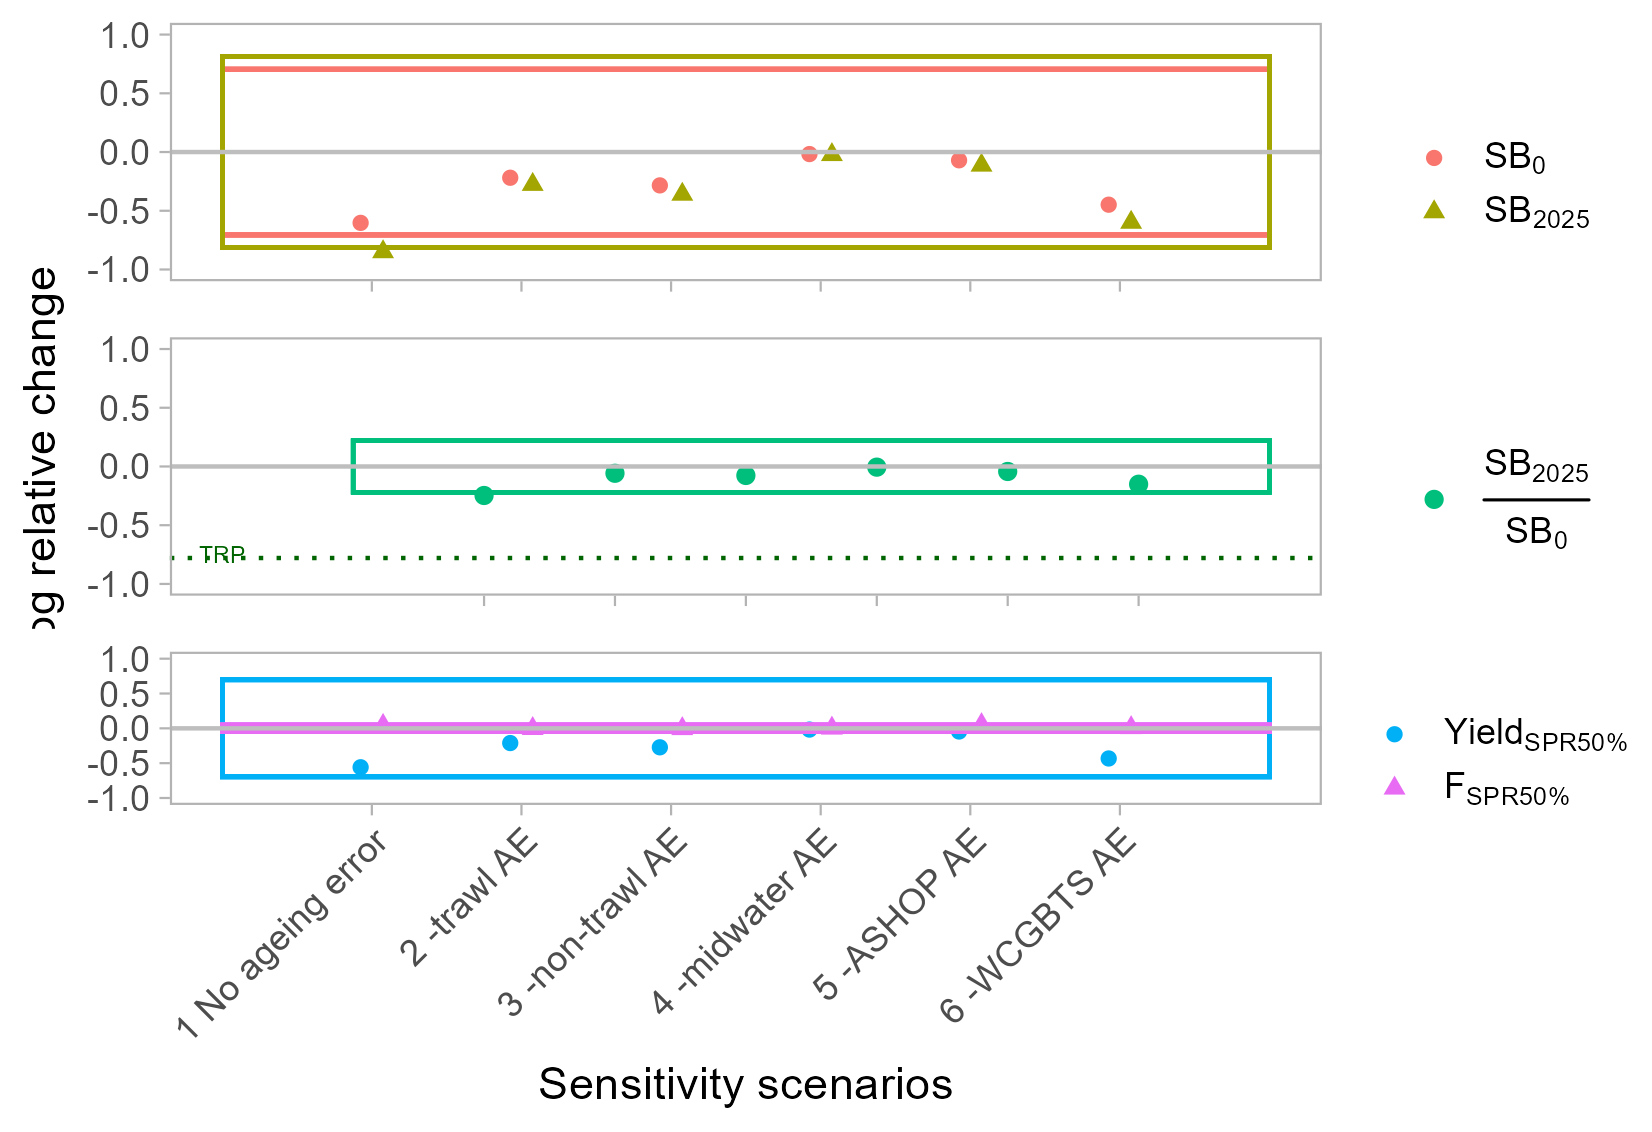
\includegraphics{Sensis/data_sensitivities/Sensi_logREplot_SB_Dep_F_Yield_AE.png}

}

\caption{\label{fig-sensi-RE-ageing-error}Log relative change
(log((Model\_sensi-Model\_ref)/Model\_ref)) in ageing error scenarios
for 5 derived quantities. Colored boxes indicate 95 percent confidence
interval of the reference model. See `Sensitivity Analysis' section for
more details on each scenario.}

\end{figure}%

\begin{figure}[H]

\centering{

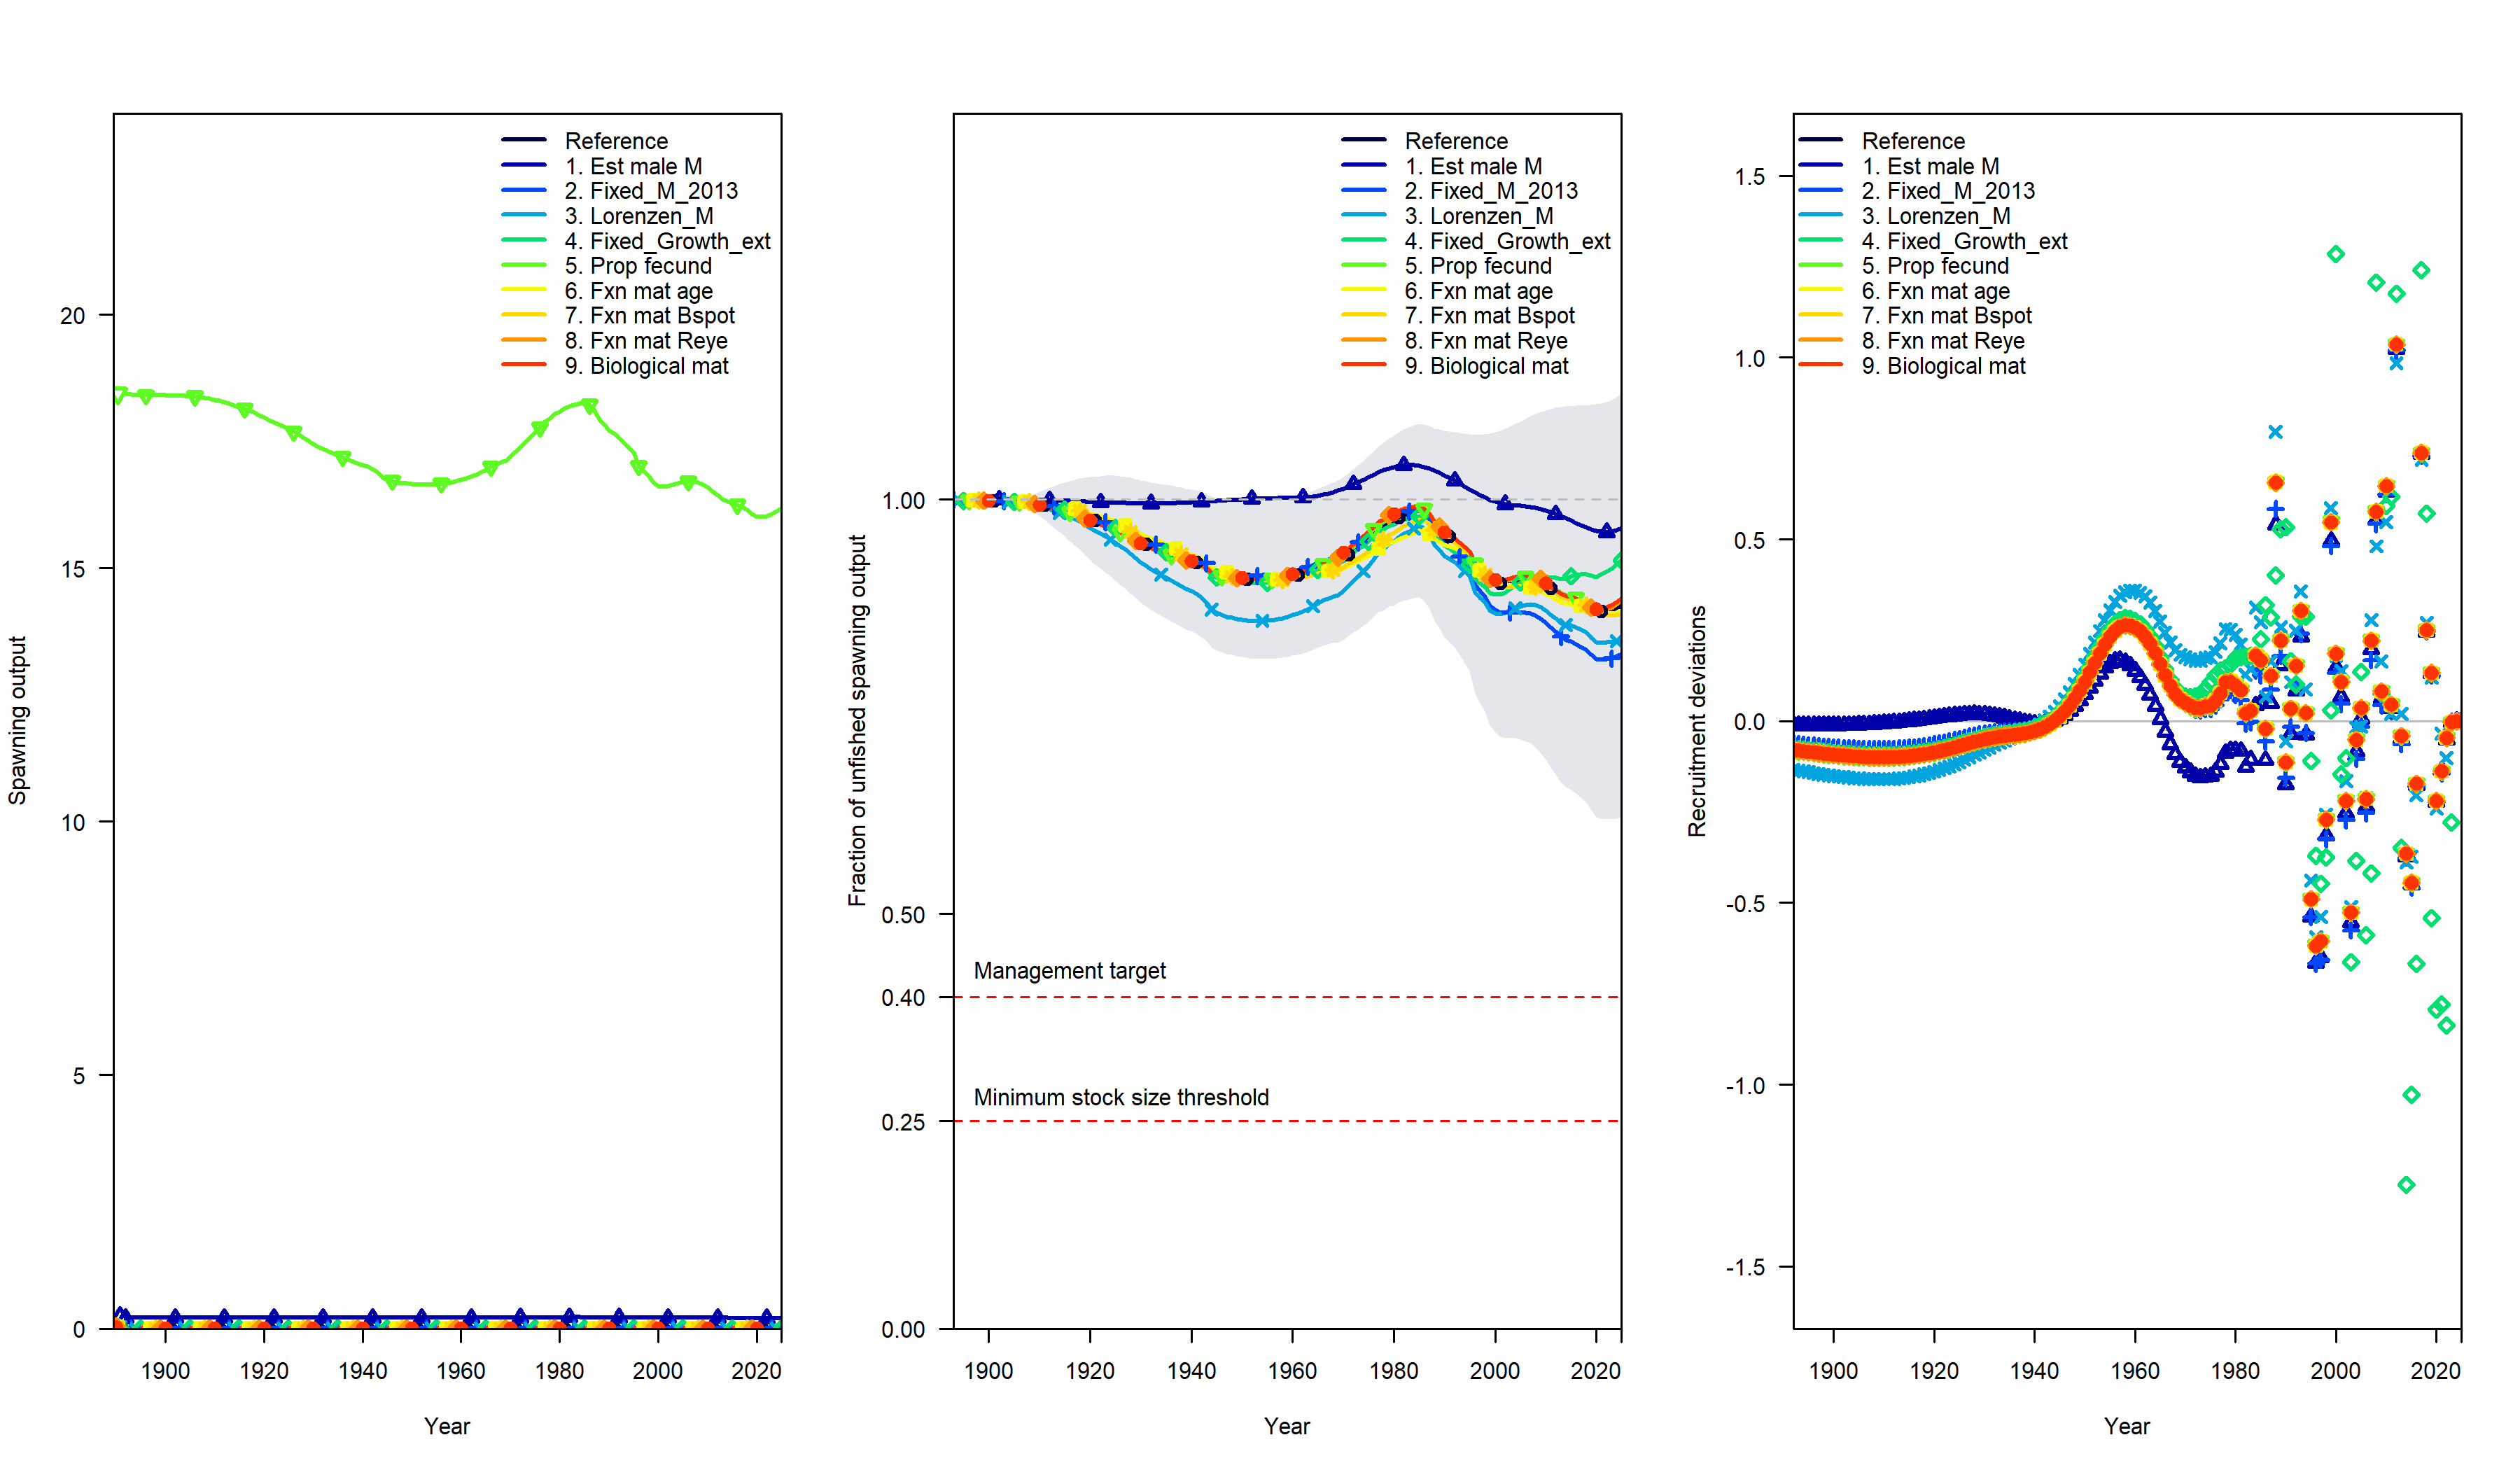
\includegraphics{Sensis/model_specs/M_Gr_Reproduction.png}

}

\caption{\label{fig-sensi-LH}Comparison of spawning output (trillions of
eggs; left panel), relative stock status (middle panel) and recruitment
estimation (right panel) for models under different natural mortality,
growth and reproductive biology scenarios.}

\end{figure}%

\begin{figure}[H]

\centering{

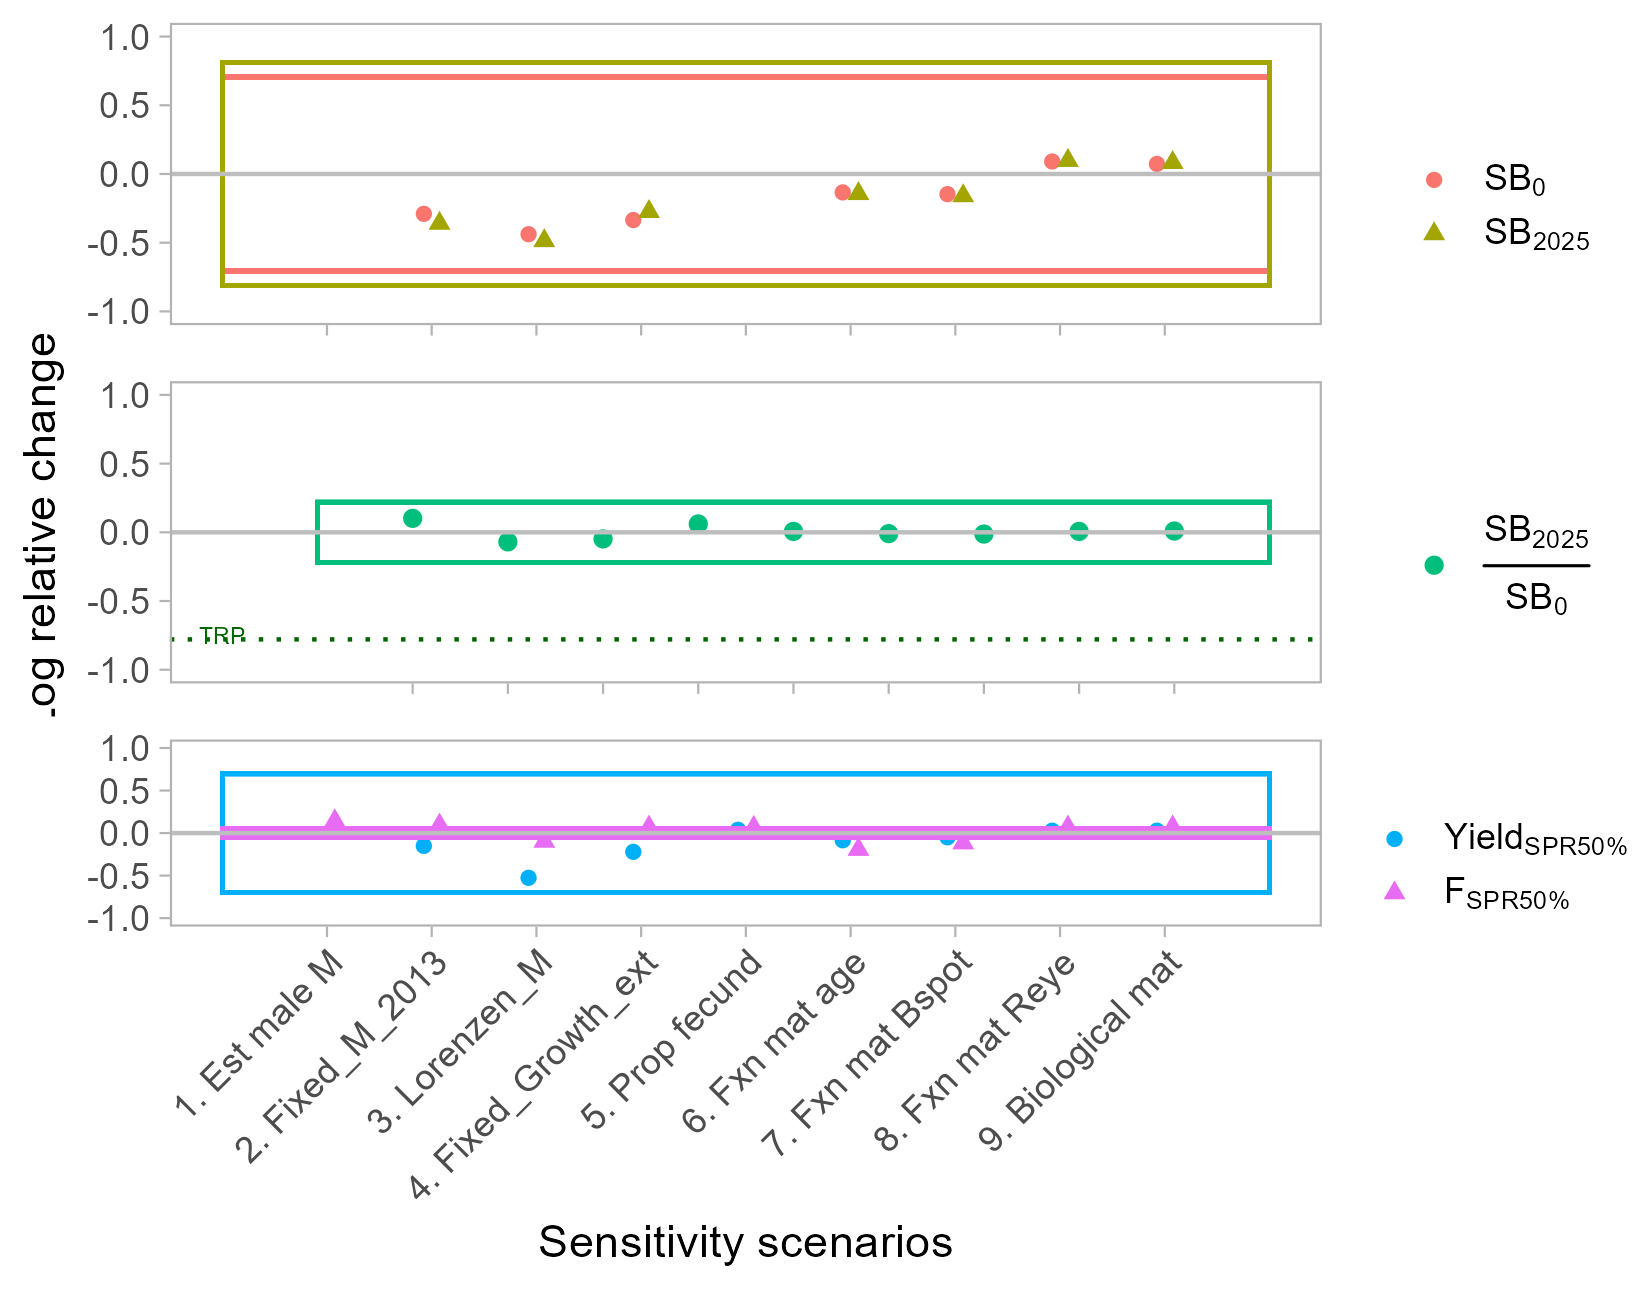
\includegraphics{Sensis/model_specs/Sensi_logREplot_SB_Dep_F_Yield_MGrRep.png}

}

\caption{\label{fig-sensi-RE-LH}Log relative change
(log((Model\_sensi-Model\_ref)/Model\_ref)) in natural mortality, growth
and reproductive biology scenarios for 5 derived quantities. Colored
boxes indicate 95 percent confidence interval of the reference model.
See `Sensitivity Analysis' section for more details on each scenario.}

\end{figure}%

\begin{figure}[H]

\centering{


\includegraphics{Sensis/model_specs/compare1_spawnbio.png}

}

\caption{\label{fig-sensi-LH-so}Comparison of spawning output (trillions
of eggs) for models under different natural mortality, growth and
reproductive biology scenarios. This comparison excludes the model
estimating natural mortality, as the scale goes extremely high, and the
weight proportional to fecundity scenario, as it is on a different scale
than the other models.}

\end{figure}%

\begin{figure}[H]

\centering{

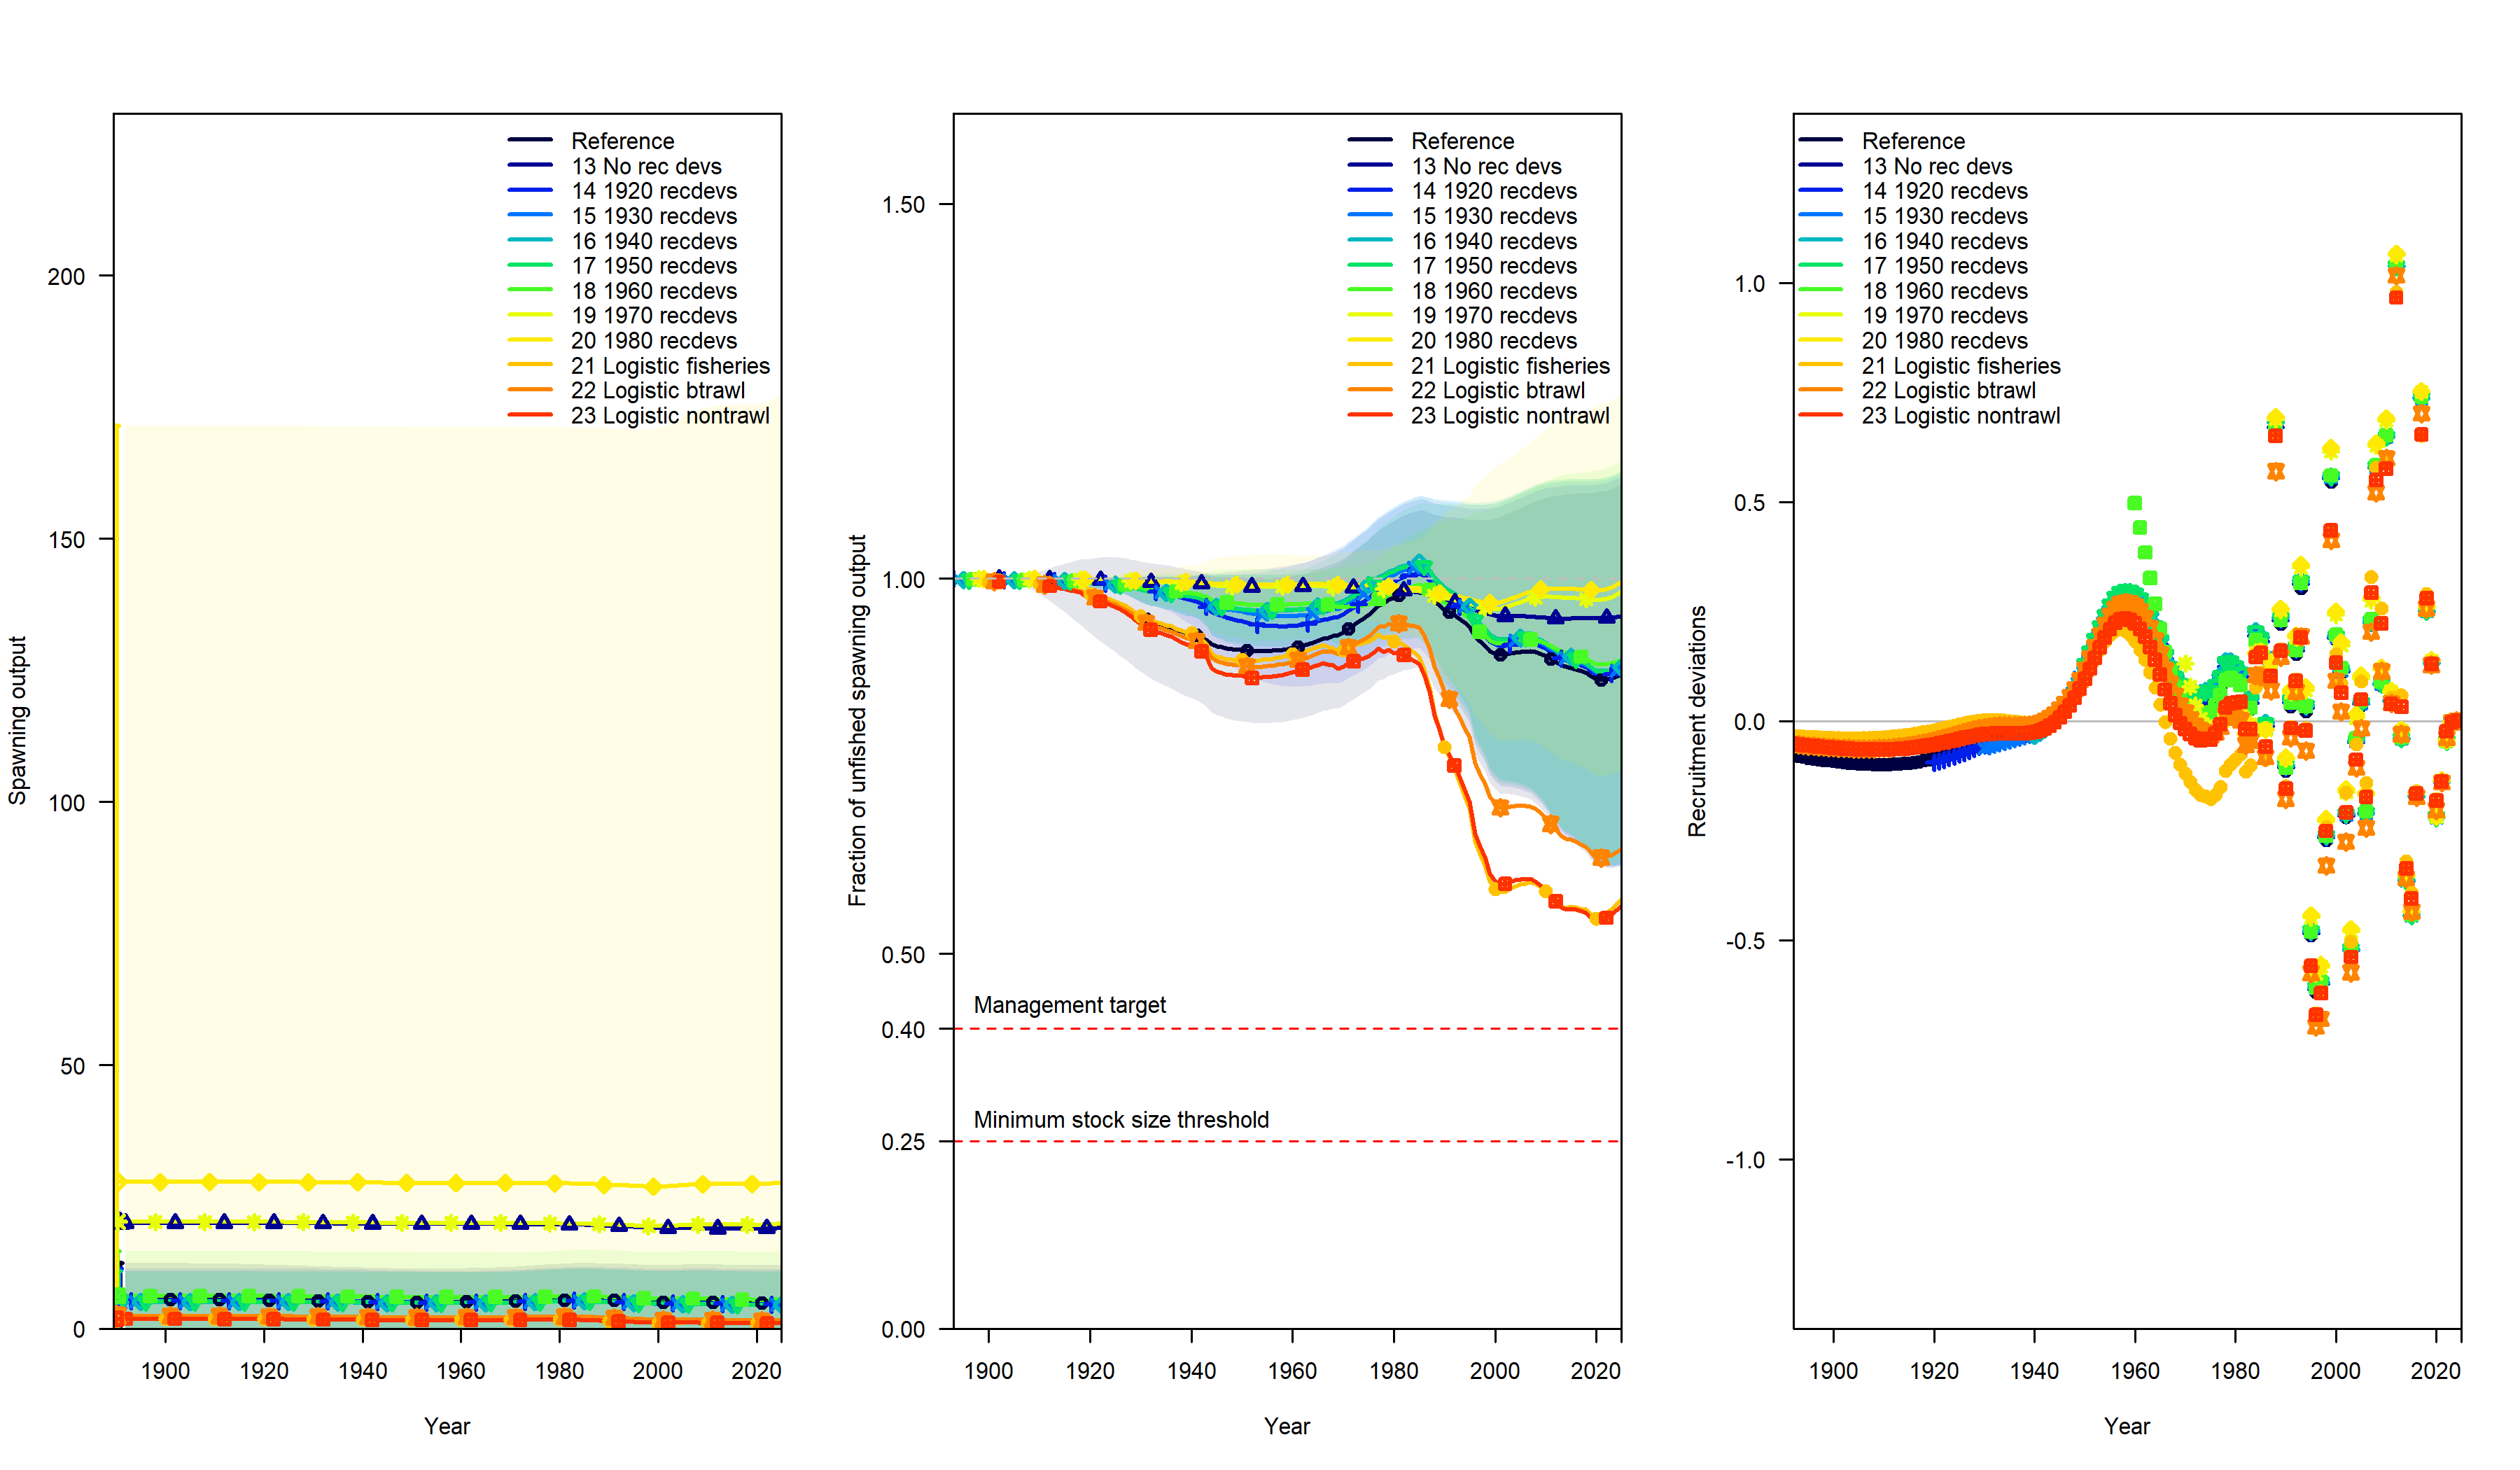
\includegraphics{Sensis/model_specs/Sel_Rec.png}

}

\caption{\label{fig-sensi-SelRec}Comparison of spawning output
(trillions of eggs; left panel), relative stock status (middle panel)
and recruitment estimation (right panel) for models under different
recruitment and selectivity scenarios.}

\end{figure}%

\begin{figure}[H]

\centering{

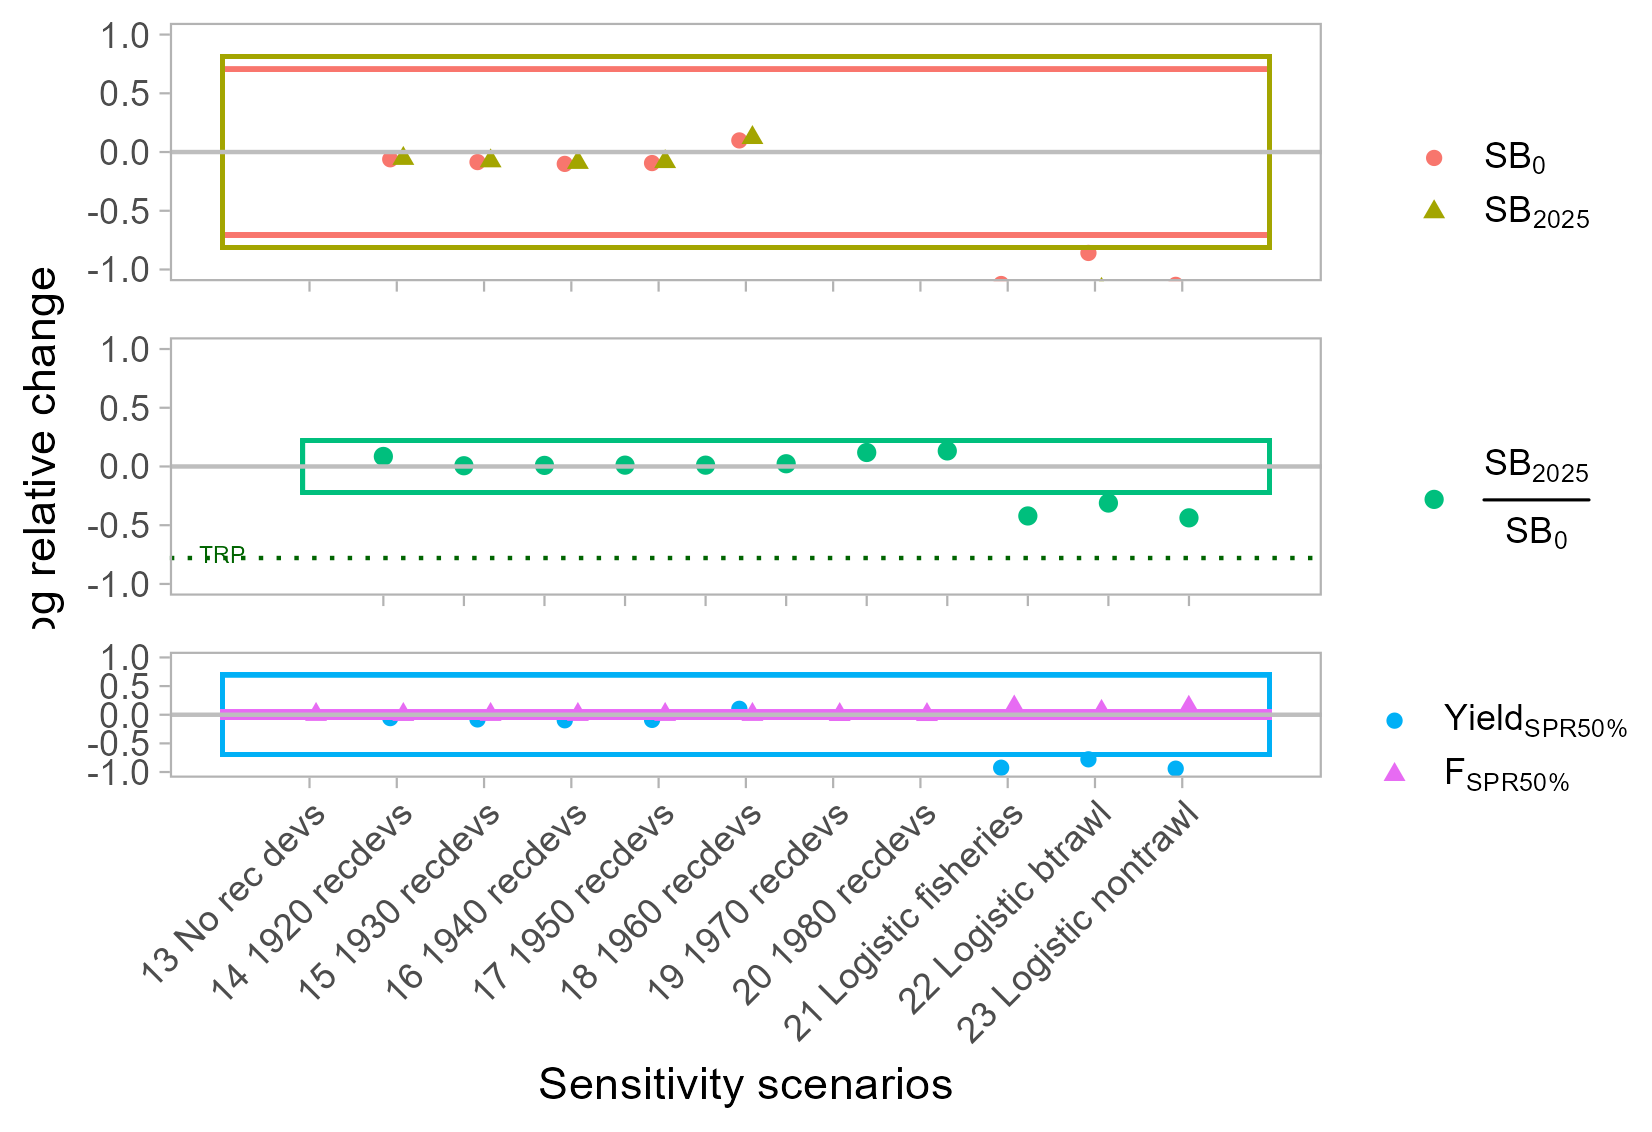
\includegraphics{Sensis/model_specs/Sensi_logREplot_SB_Dep_F_Yield_Sel_Rec.png}

}

\caption{\label{fig-sensi-RE-SelRec}Log relative change
(log((Model\_sensi-Model\_ref)/Model\_ref)) in recruitment and
selectivity scenarios for 5 derived quantities. Colored boxes indicate
95 percent confidence interval of the reference model. See `Sensitivity
Analysis' section for more details on each scenario.}

\end{figure}%

\begin{figure}[H]

\centering{

\includegraphics{Sensis/model_specs/comp_lenfit__aggregated_across_time_logsel.png}

}

\caption{\label{fig-sensi-logsel_fits}Aggregate fit to length
compositions for the scenario that assume logistic selectivity for all
fisheries and time blocks.}

\end{figure}%

\newpage

\subsection{Likelihood Profiles}\label{likelihood-profiles}

\begin{figure}[H]

\centering{

\includegraphics{Like_profiles/lnR0/parameter_panel_SR_LN(R0).png}

}

\caption{\label{fig-likeprof-lnR0-parm}Initial recruitment (\(lnR_0\))
likelihood profile (change in the negative log-likelihood across a range
of \(ln(R0)\) values) and derived quantities. Red line in the top left
figure indicates the significance level in likelihood difference.}

\end{figure}%

\begin{figure}[H]

\centering{

\includegraphics{Like_profiles/lnR0/piner_panel_SR_LN(R0).png}

}

\caption{\label{fig-likeprof-lnR0-components}Initial recruitment
(\(ln(R0)\)) likelihood profile for each of the likelihood components.}

\end{figure}%

\begin{figure}[H]

\centering{

\includegraphics{Like_profiles/Steepness/parameter_panel_SR_BH_steep.png}

}

\caption{\label{fig-likeprof-h-parm}Steepness (\(h\)) likelihood profile
(change in the negative log-likelihood across a range of \(h\) values)
and derived quantities. Red line in the top left figure indicates the
significance level in likelihood difference.}

\end{figure}%

\begin{figure}[H]

\centering{

\includegraphics{Like_profiles/Steepness/piner_panel_SR_BH_steep.png}

}

\caption{\label{fig-likeprof-h-components}Steepness (\(h\)) likelihood
profile for each of the likelihood components.}

\end{figure}%

\begin{figure}[H]

\centering{

\includegraphics{Like_profiles/Male_M/parameter_panel_NatM_uniform_Mal_GP_1.png}

}

\caption{\label{fig-likeprof-M-parm}Male natural mortality (\(M\))
likelihood profile (change in the negative log-likelihood across a range
of male \(M\) values) and derived quantities. Red line in the top left
figure indicates the significance level in likelihood difference.}

\end{figure}%

\begin{figure}[H]

\centering{

\includegraphics{Like_profiles/Male_M/M_sex.png}

}

\caption{\label{fig-likeprof-M-sex}Likelihood differences by natural
mortality (\(M\)) by sex.}

\end{figure}%

\begin{figure}[H]

\centering{

\includegraphics{Like_profiles/Male_M/piner_panel_NatM_uniform_Mal_GP_1.png}

}

\caption{\label{fig-likeprof-M-components}Male natural mortality (\(M\))
likelihood profile for each of the likelihood components.}

\end{figure}%

\subsection{States of Nature}\label{states-of-nature}

\begin{figure}[H]

\centering{

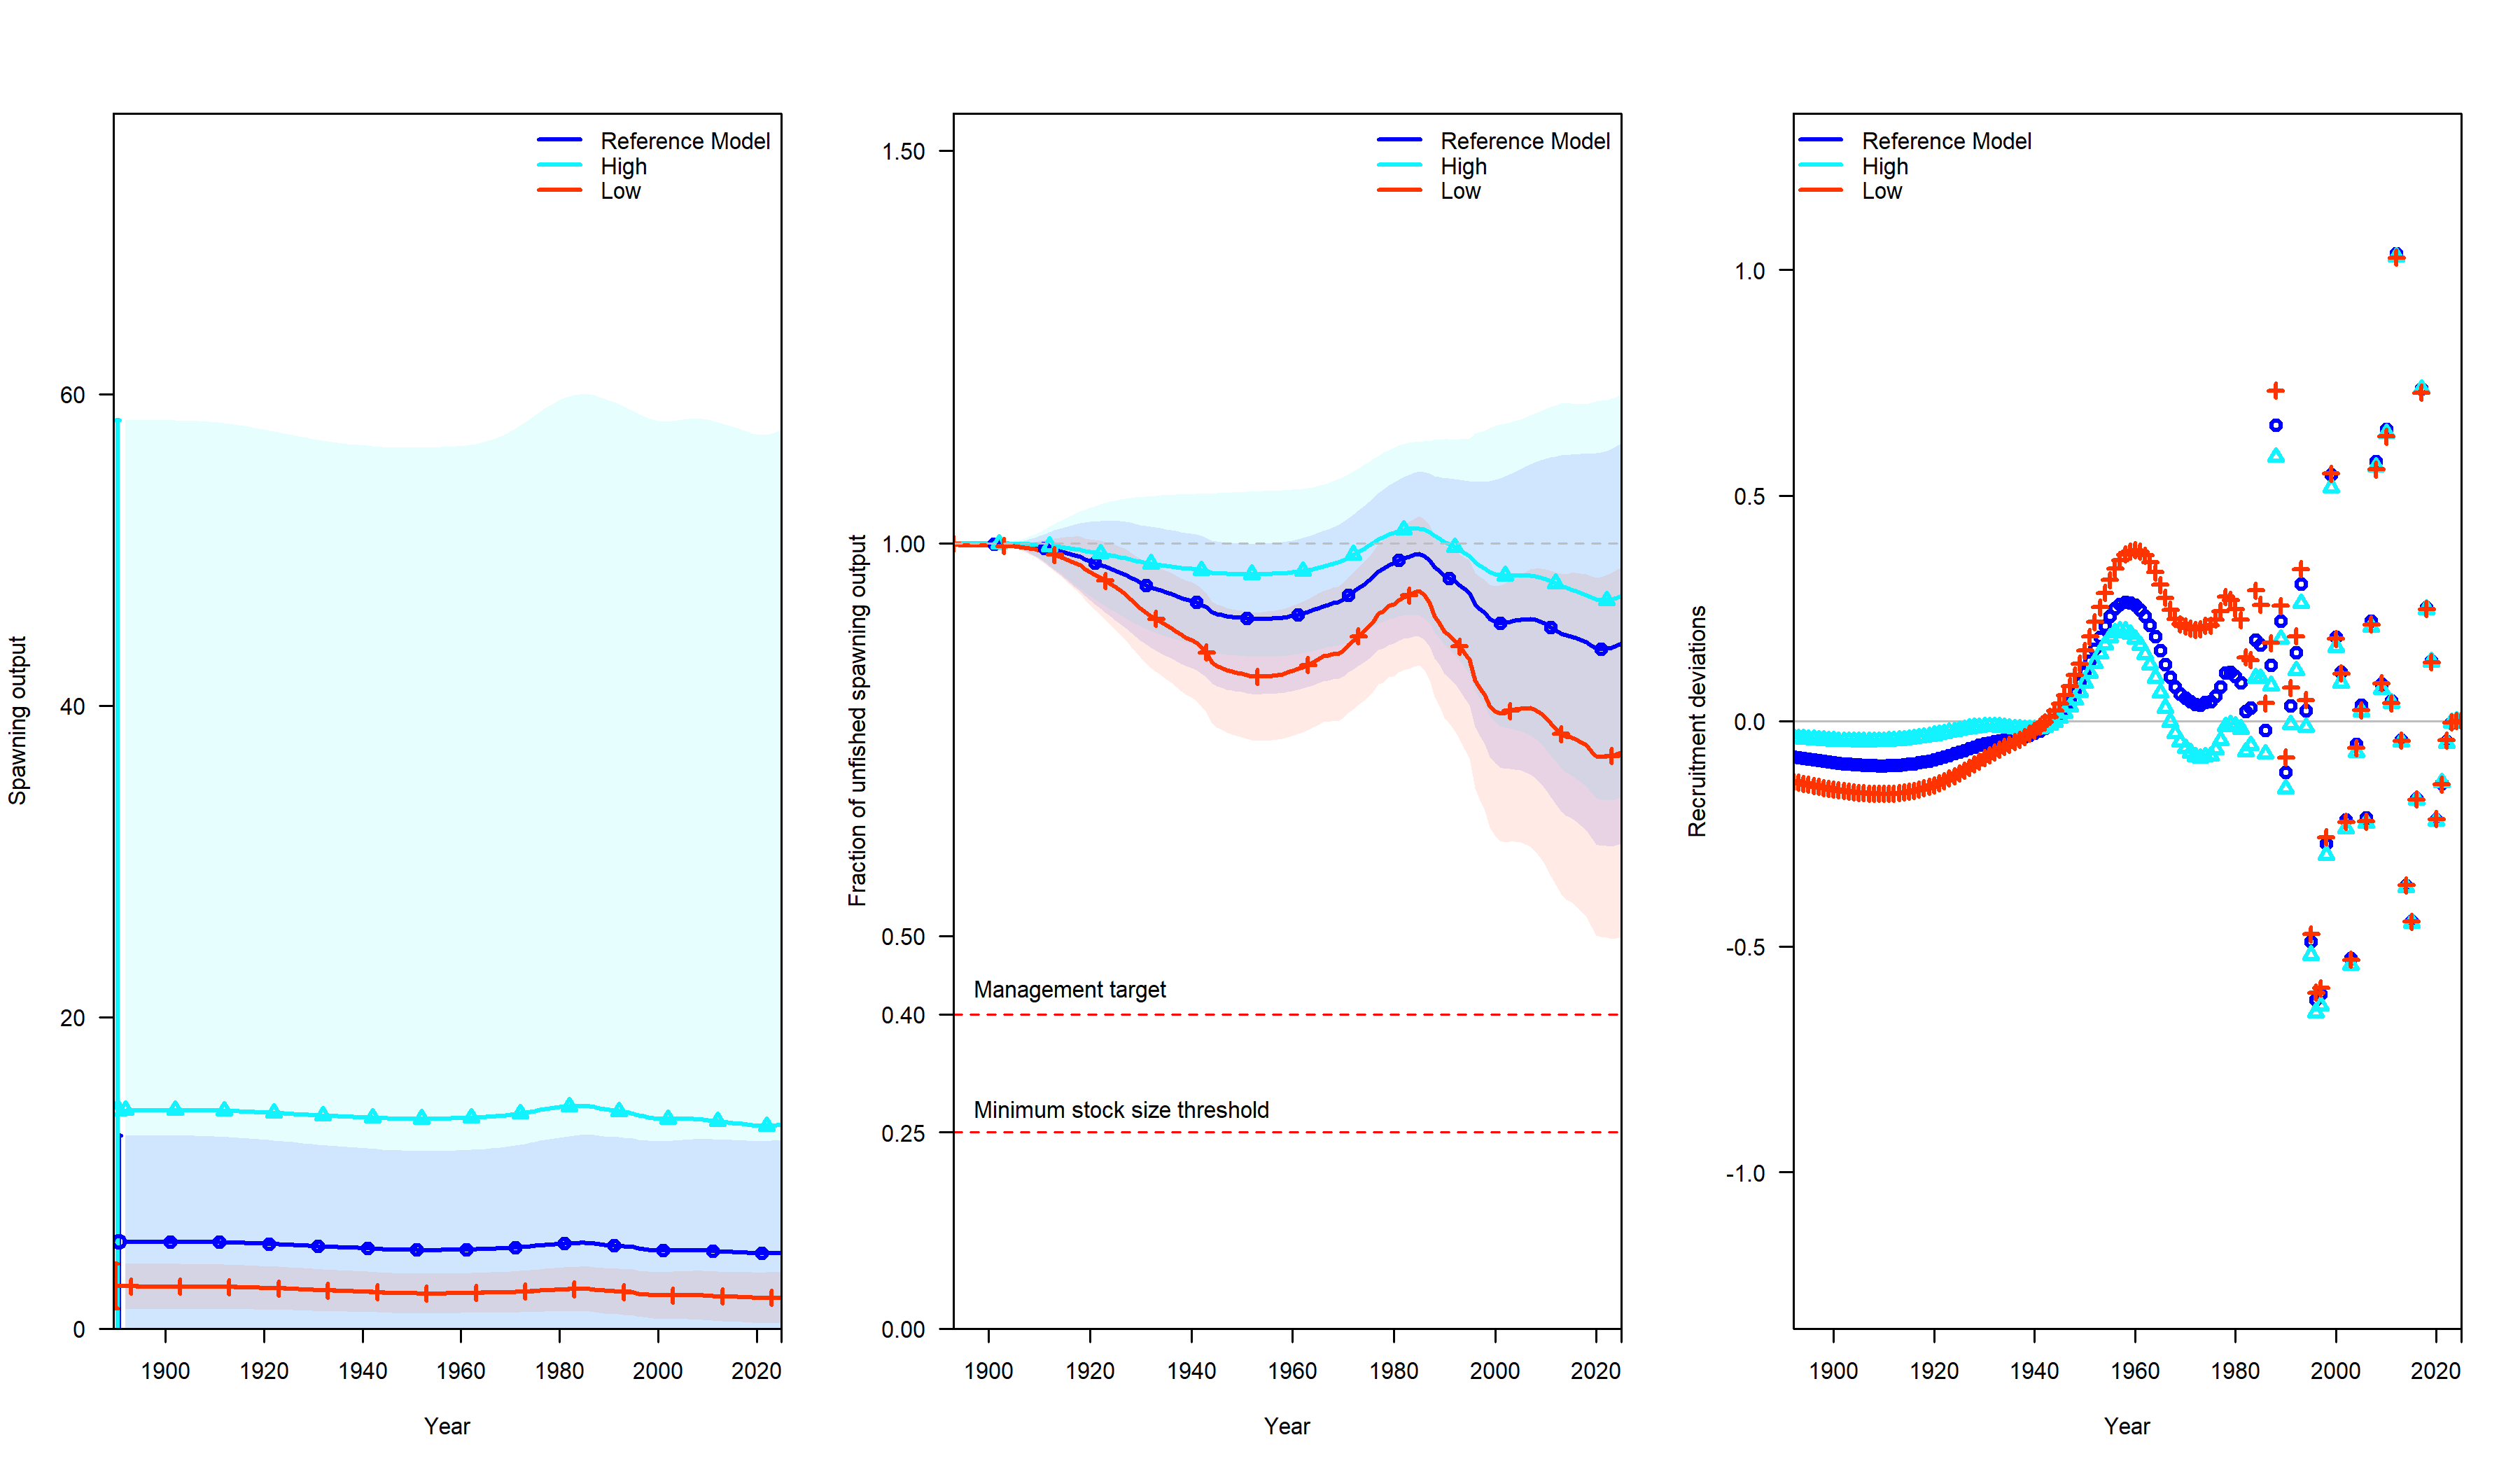
\includegraphics{Sensis/statesofnature/StatesofNature.png}

}

\caption{\label{fig-states-of-nature}Comparison of spawning output
(trillions of eggs; left panel), relative stock status (middle panel)
and recruitment estimation (right panel) for the reference model and
high and low states of nature.}

\end{figure}%

\newpage

\begin{figure}[H]

\centering{

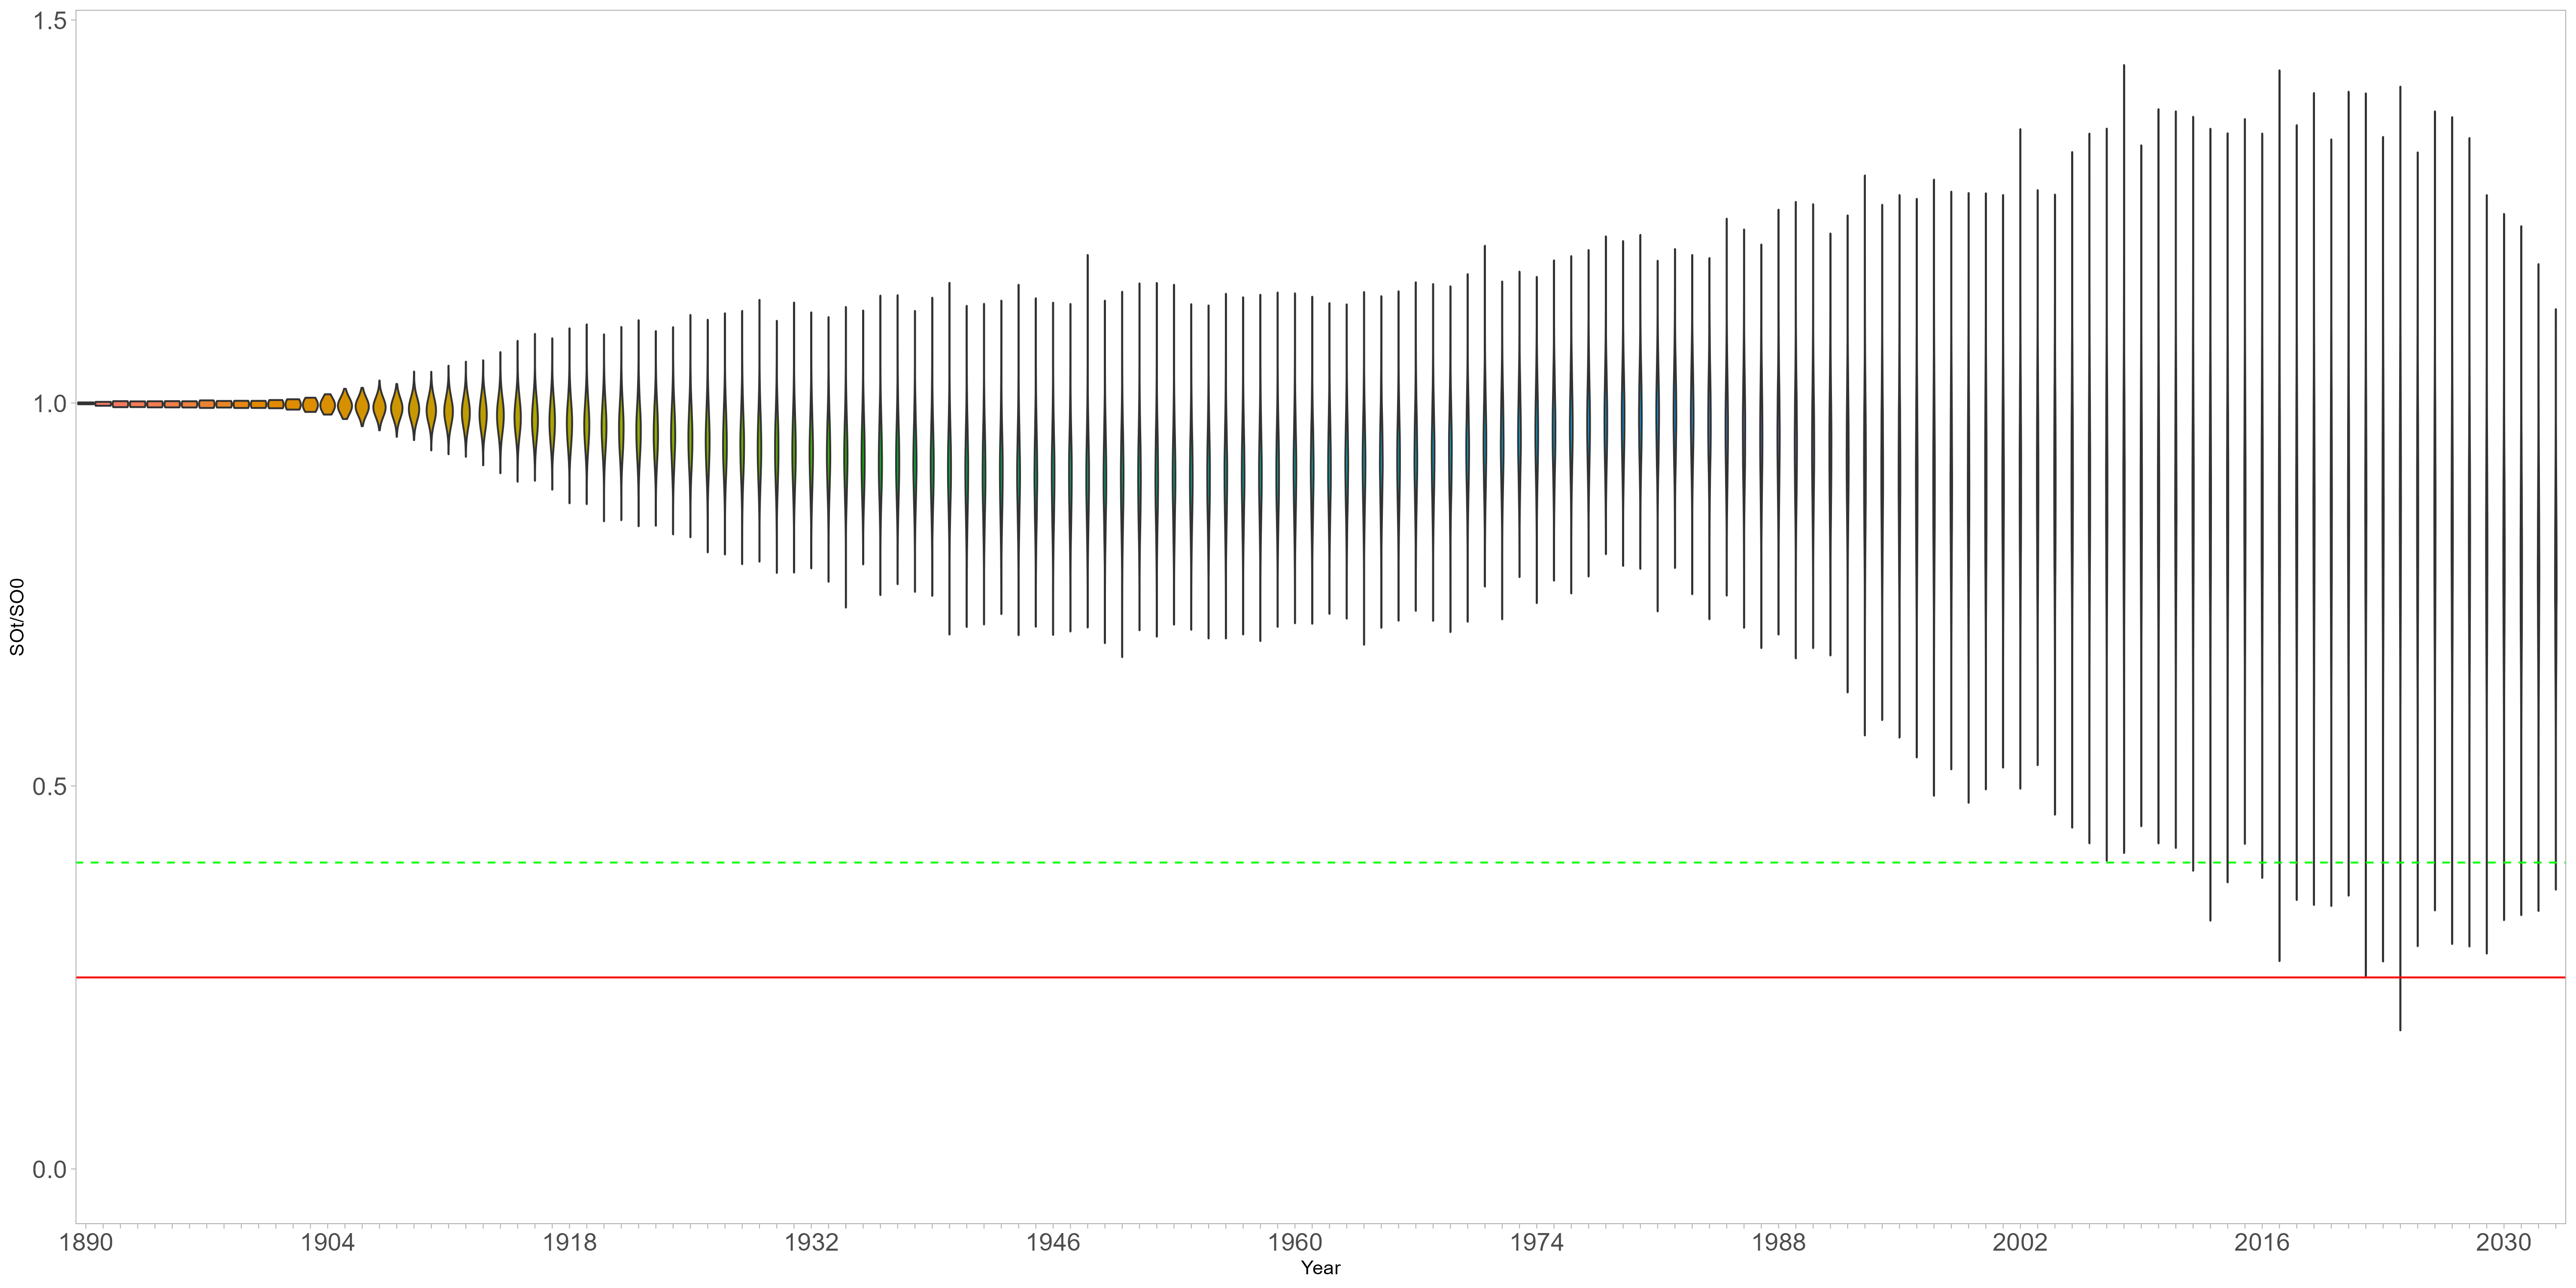
\includegraphics{Sensis/statesofnature/Ensemble_Bratio.png}

}

\caption{\label{fig-ensemble}Ensemble relative stock status for the
reference model and two states of nature.}

\end{figure}%

\begin{figure}[H]

\centering{

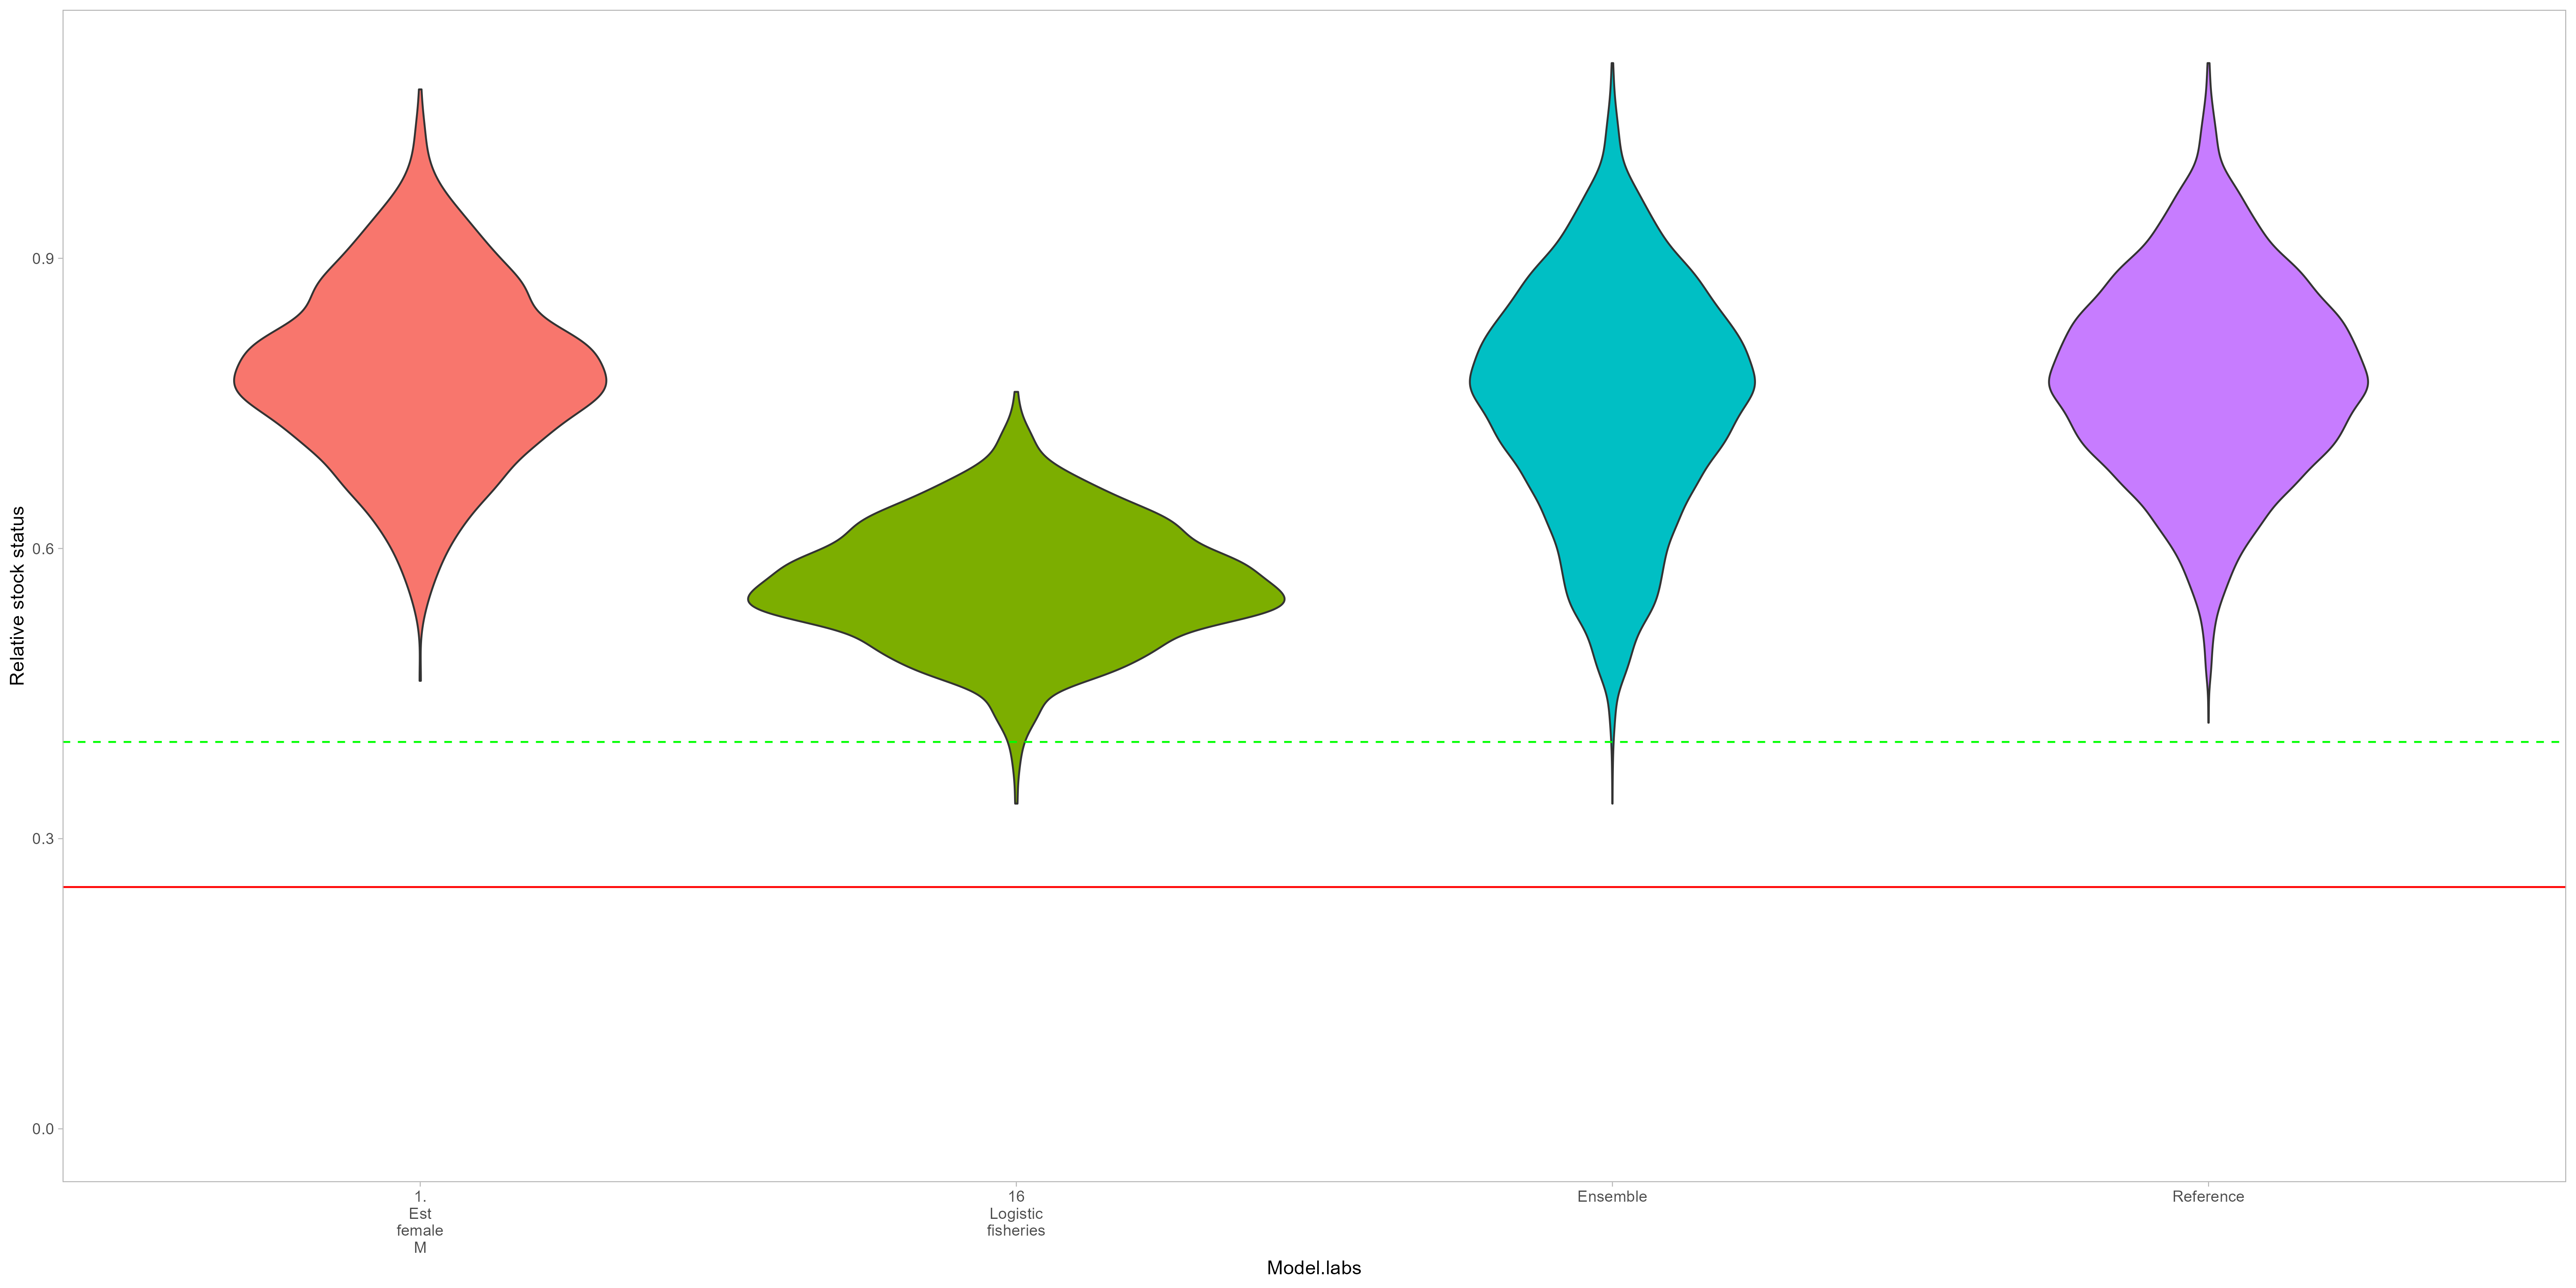
\includegraphics{Sensis/statesofnature/Ensemble_comp_plots_RSS.png}

}

\caption{\label{fig-ensemble-violin}Ensemble terminal year relative
stock status for the reference model and two states of nature.}

\end{figure}%

\newpage

\begin{figure}[H]

\centering{

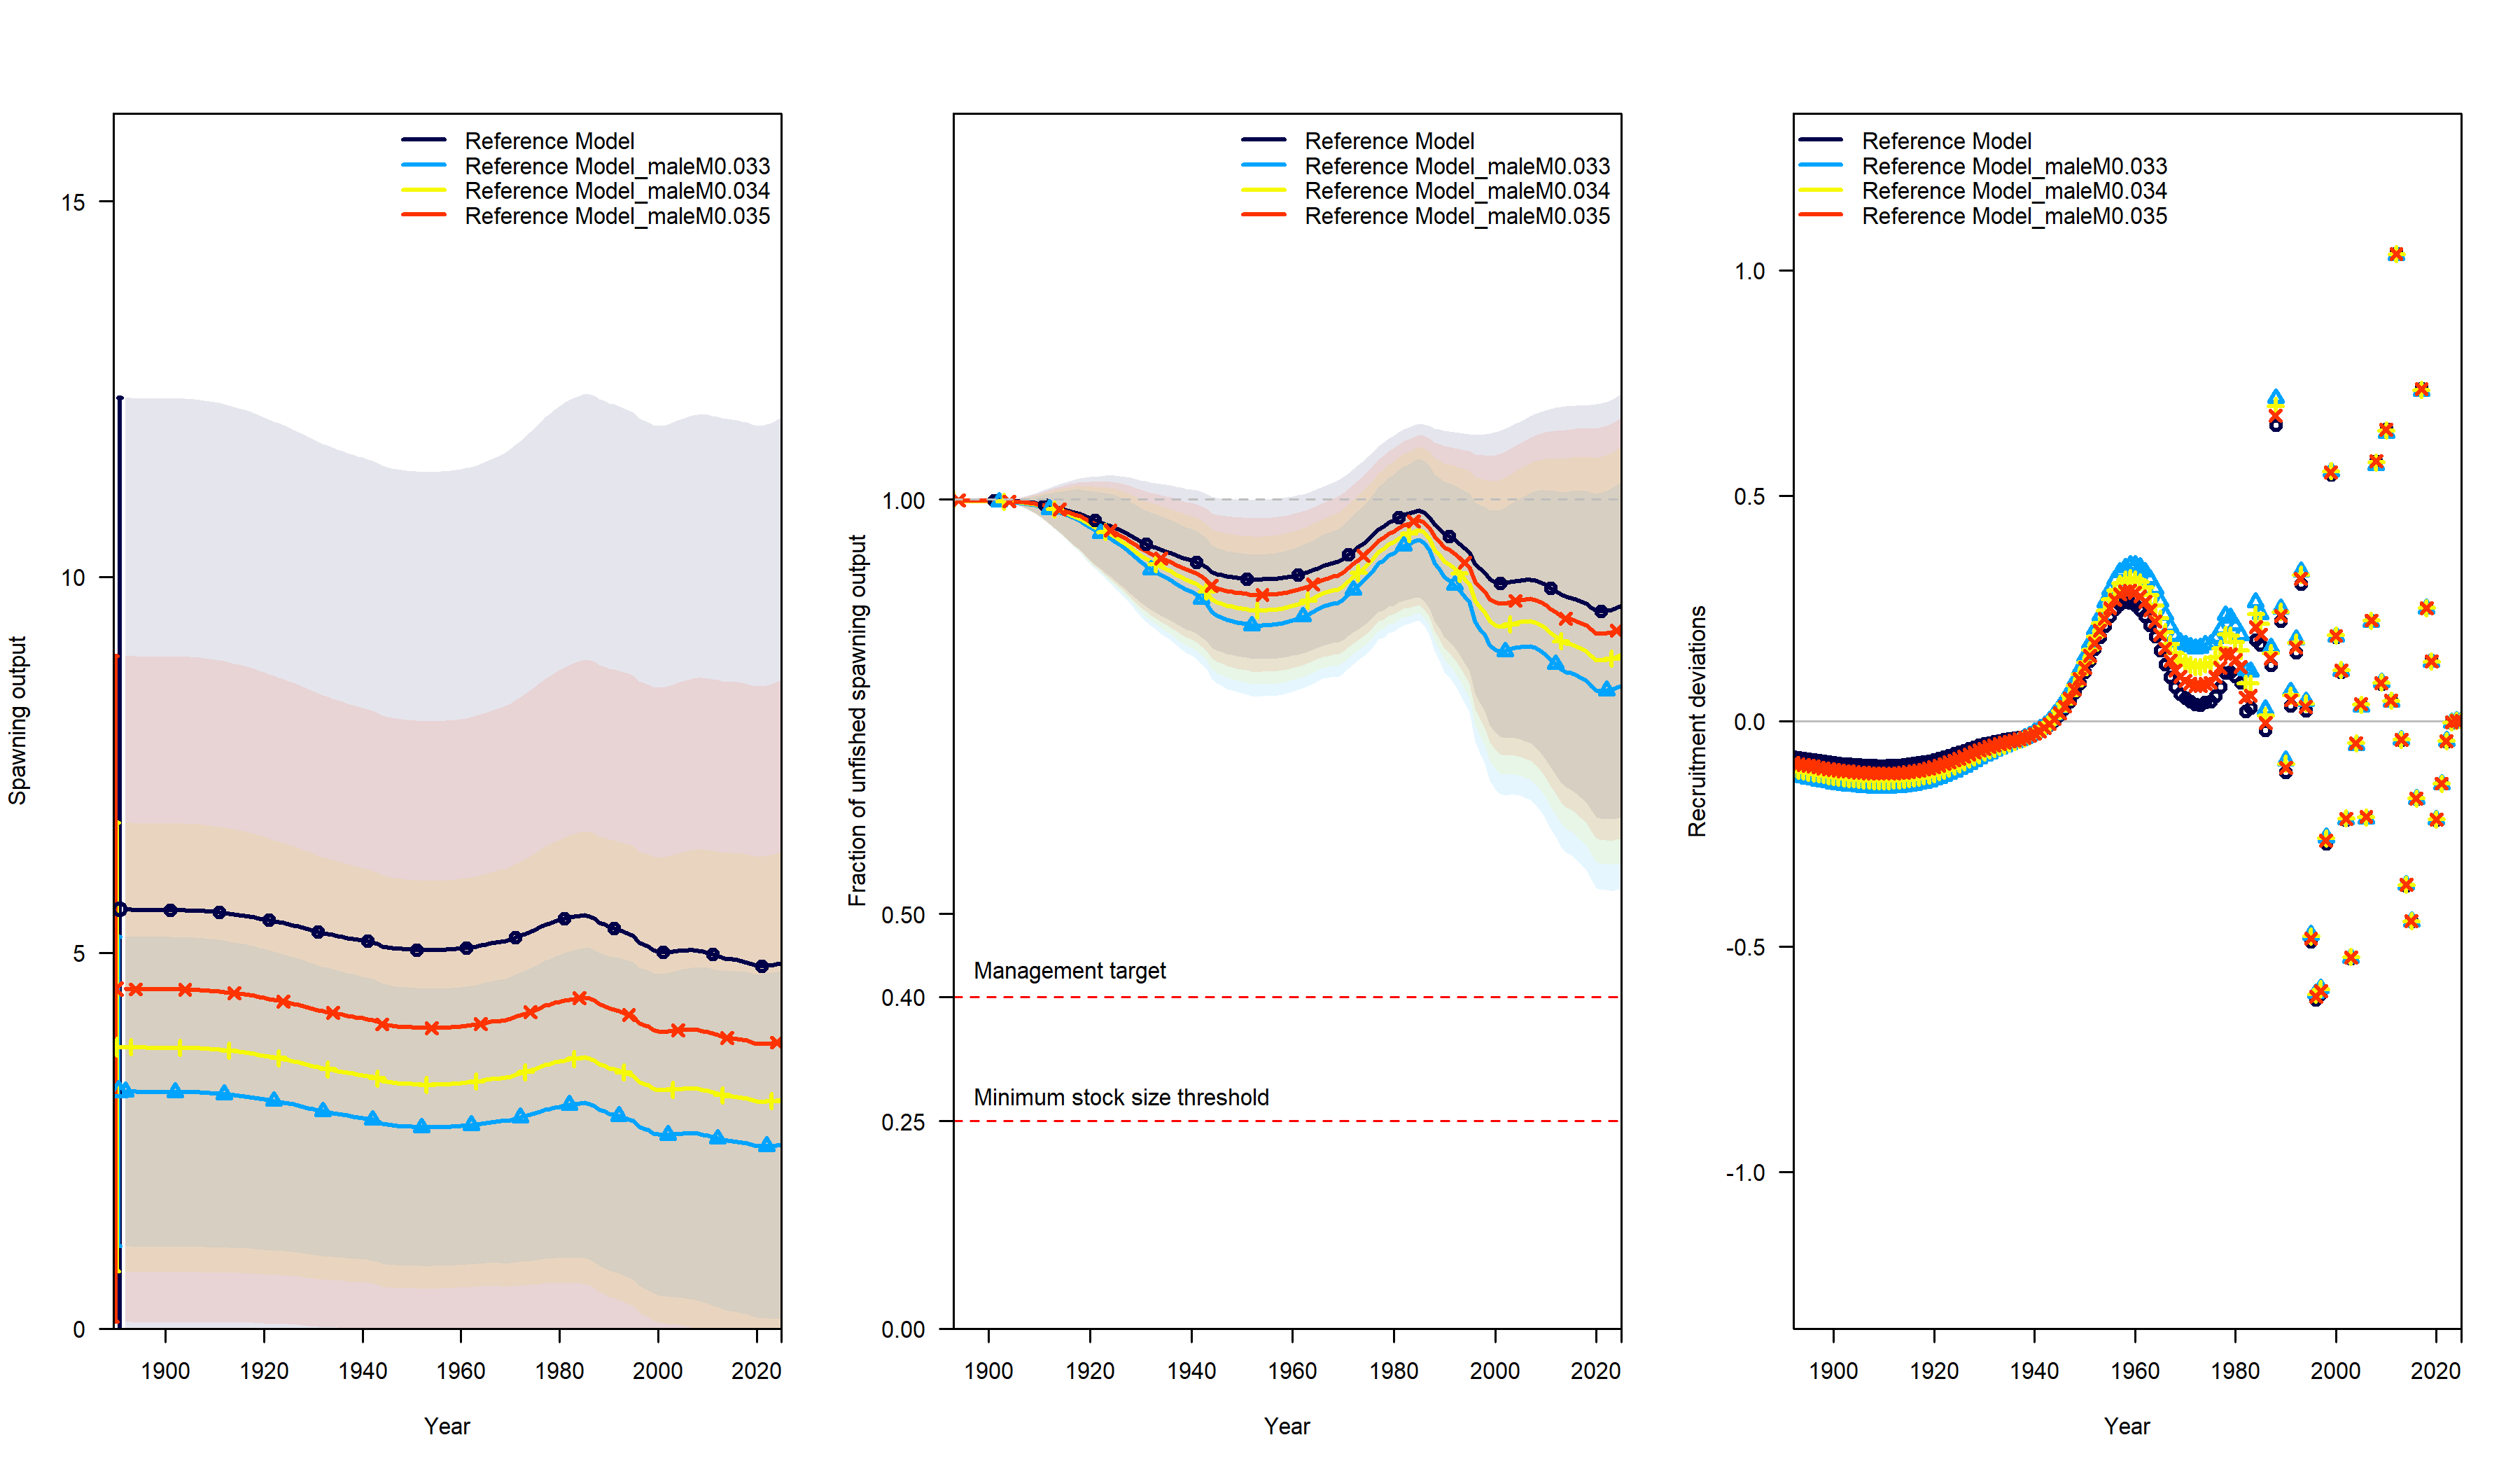
\includegraphics{Sensis/model_specs/Reduced uncertainty comparison.png}

}

\caption{\label{fig-uncert-decrease}Comparison of spawning output
(trillions of eggs; left panel), relative stock status (middle panel)
and recruitment estimation (right panel) for the reference model and
models that decrease the pre-specified male natural mortality value.
Note the decreasing uncertainty in scale as the population reduces the
amount of expectation in stock status at or above unfished.}

\end{figure}%

\newpage

\newpage

\subsection{Management}\label{management-1}

\begin{figure}[H]

\centering{


\includegraphics{ref_model/plots/ts9_Relative_spawning_output_intervals.png}

}

\caption{\label{fig-management-depletion}Estimated time series of
fraction of unfished spawning output for the reference model.}

\end{figure}%

\begin{figure}[H]

\centering{

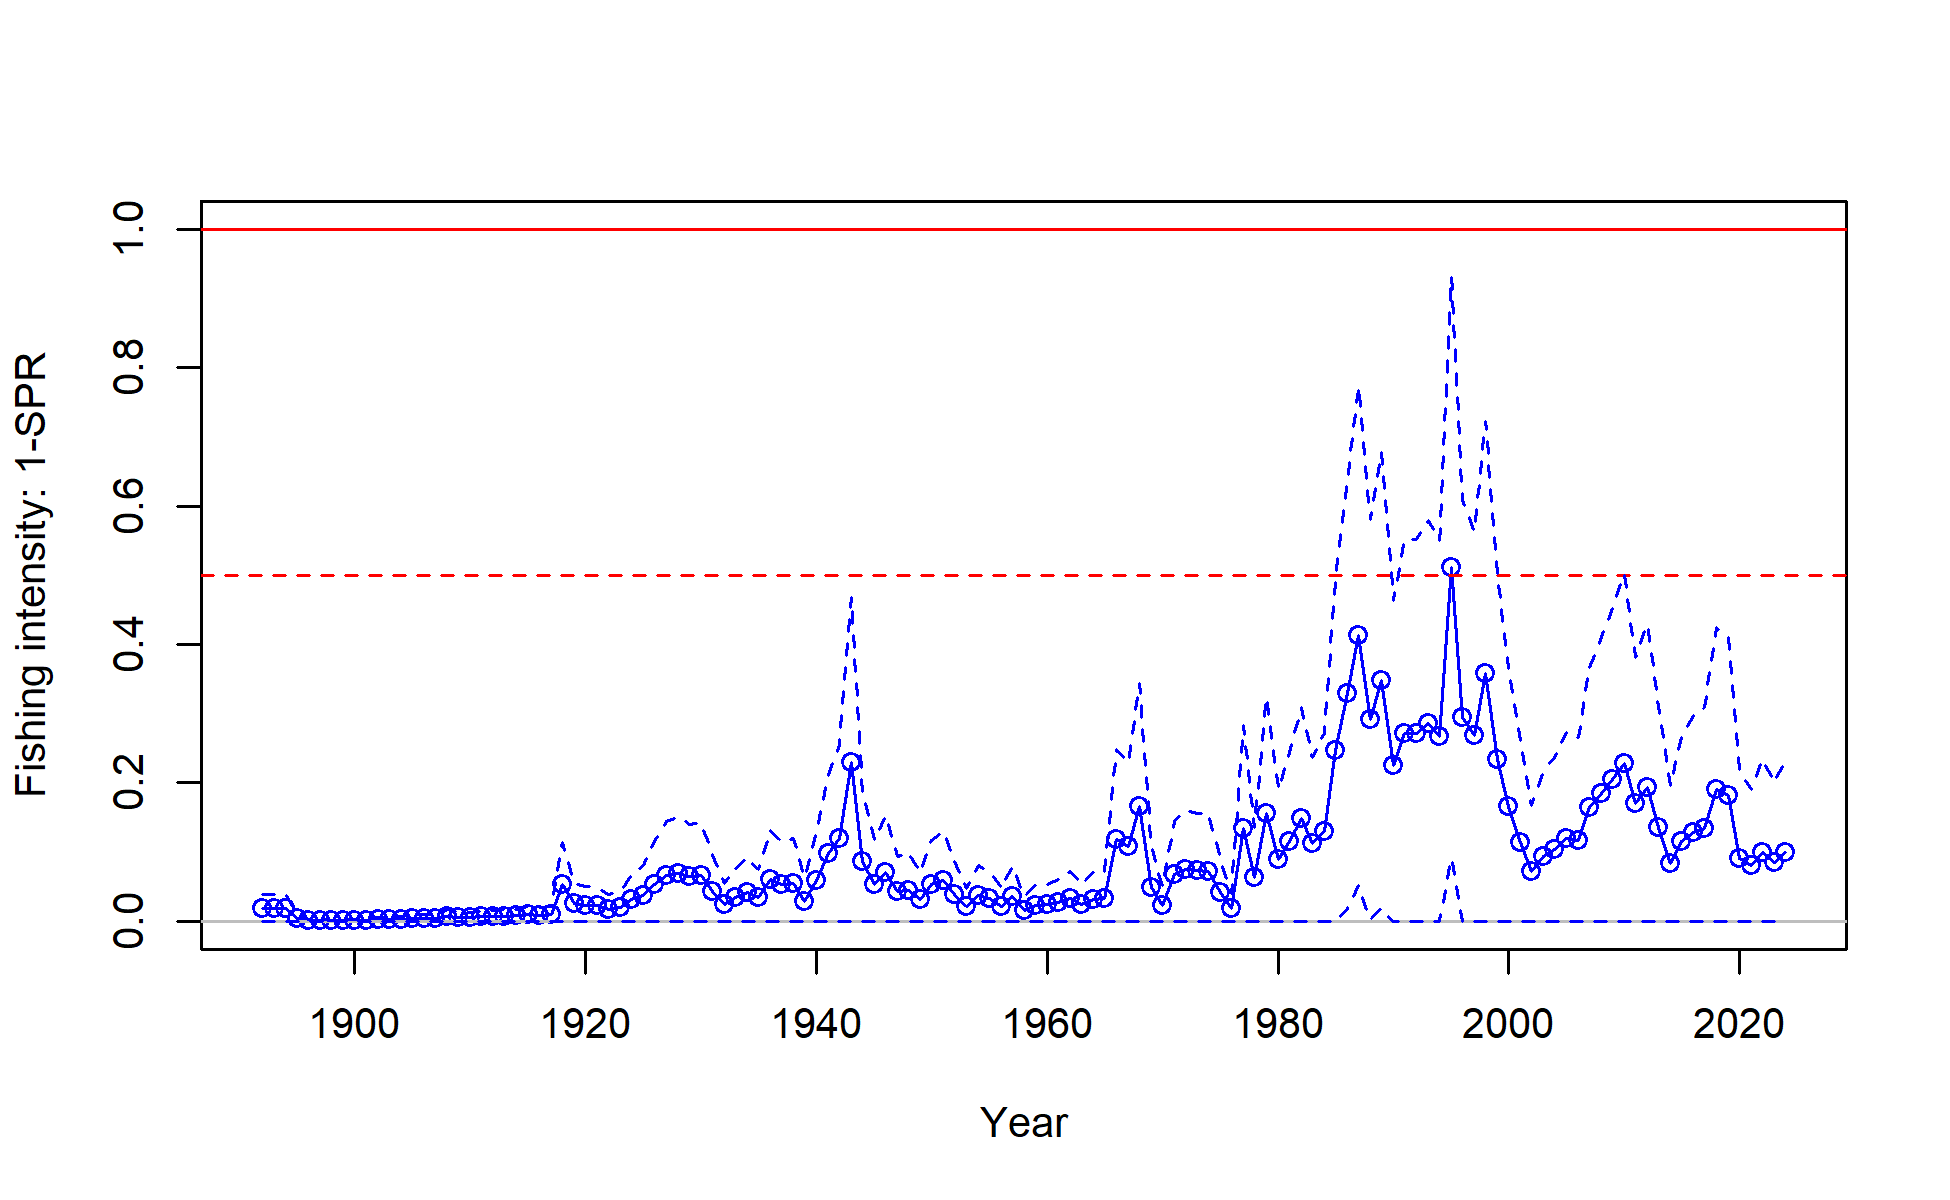
\includegraphics{ref_model/plots/SPR3_ratiointerval.png}

}

\caption{\label{fig-one-minus-spr}Estimated time series of the fishing
intensity (1 - SPR), where SPR is the spawning potential ratio, with
approximate 95\% asymptotic intervals. The horizontal line at 0.5
corresponds to SPR = 0.5, the management reference point. The horizontal
line at 1.0 corresponds to SPR = 0 (all spawning fish removed from the
population).}

\end{figure}%

\begin{figure}[H]

\centering{

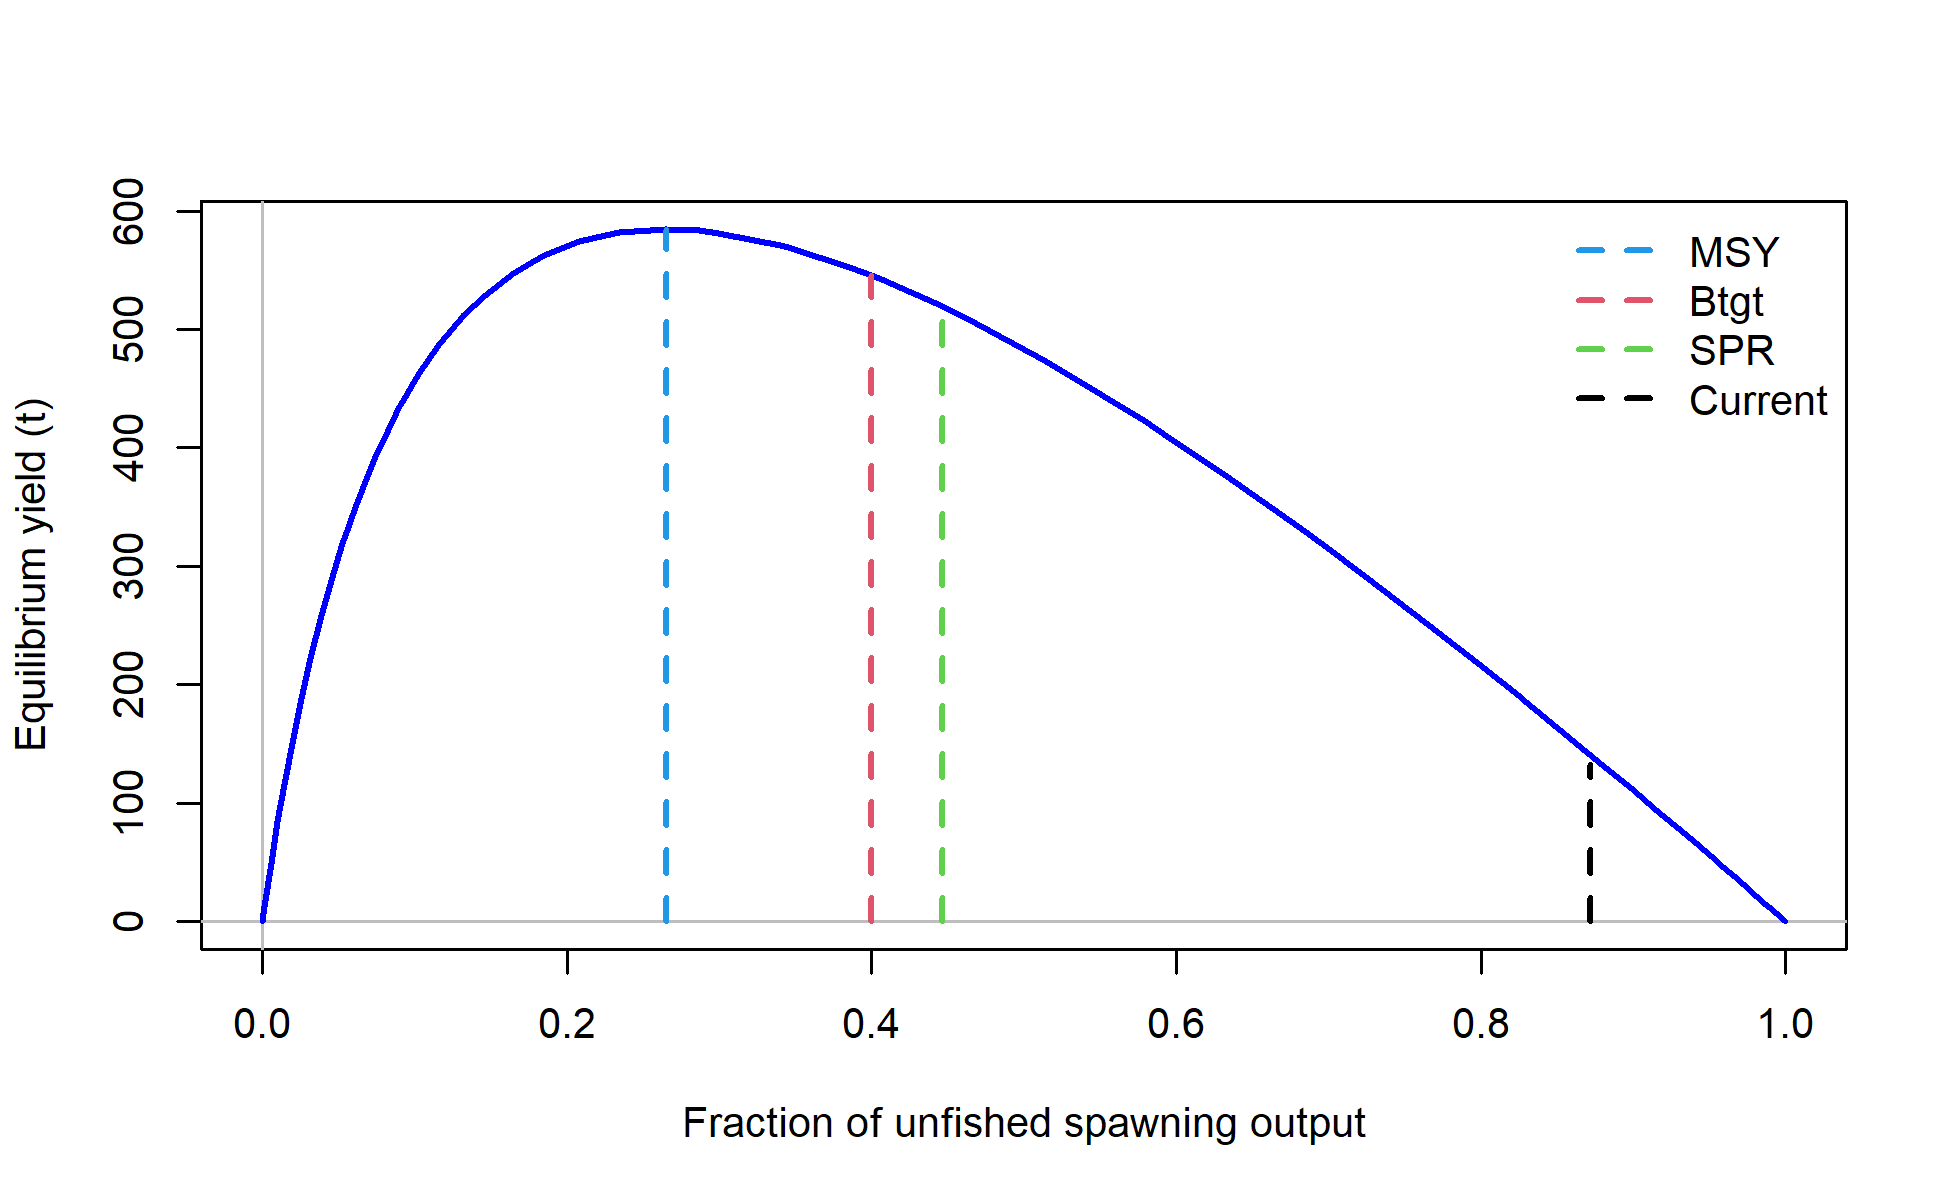
\includegraphics{ref_model/plots/yield2_yield_curve_with_refpoints.png}

}

\caption{\label{fig-management-yield}Equilibrium yield curve for the
reference model. Values are based on the most recent fishery
selectivities and retention curves and with steepness fixed at 0.72.}

\end{figure}%

\begin{figure}[H]

\centering{

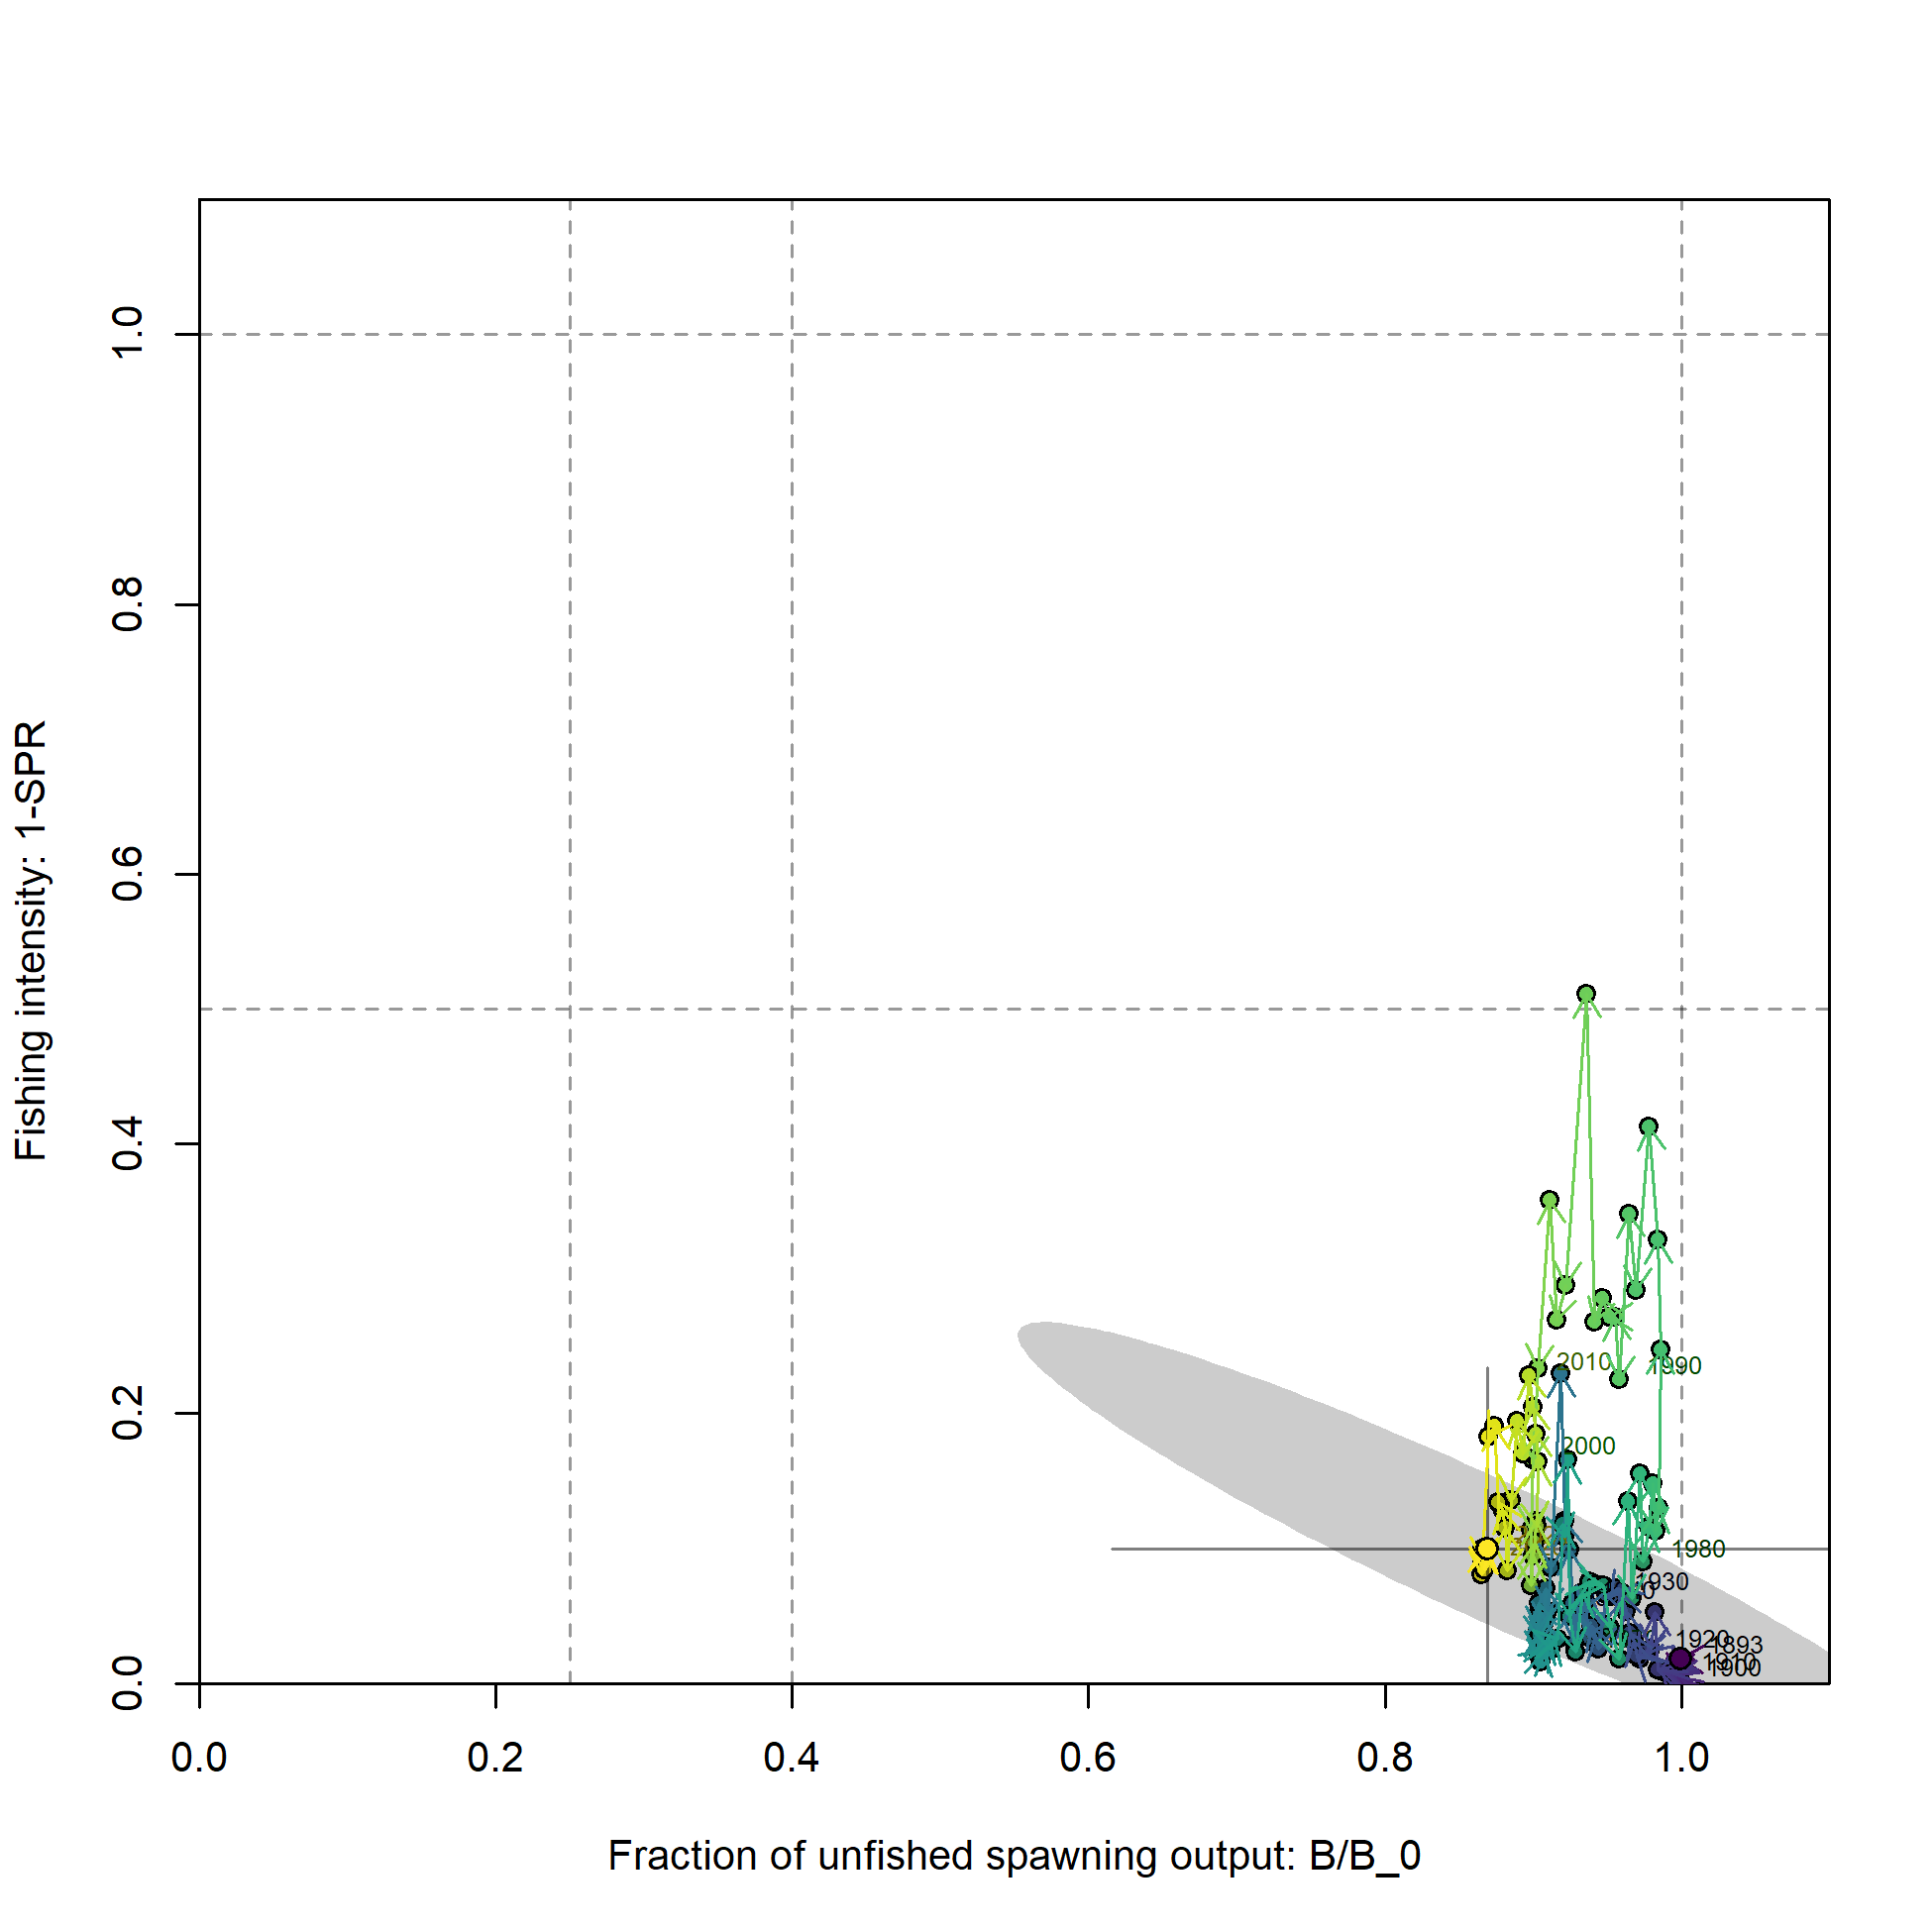
\includegraphics{ref_model/plots/SPR4_phase.png}

}

\caption{\label{fig-management-phase}Phase plot of fishing intensity
versus fraction unfished. Each point represents the biomass ratio at the
start of the year and the relative fishing intensity in that same year.
Cooler colors (purple) represent early years and warmer colors (yellow)
represent recent years. Lines through the final point show 95\%
intervals based on the asymptotic uncertainty for each dimension. The
shaded ellipse is a 95\% region which accounts for the estimated
correlation between the two quantities.}

\end{figure}%

\newpage{}

\newpage{}

\section{Appendix}\label{sec-appendix}

\subsection{Risk Table}\label{risk-table-1}

Below is a risk table for RE/BS to document 1) ecosystem and
environmental factors, 2) stock assessment data inputs, and 3)
assessment model fits and structural factors that could potentially
affect stock productivity and/or uncertainty arising from the stock
assessment (see text). Level 1 is favorable/less uncertain, Level 2
neutral, and Level 3 unfavorable/more uncertain. The risk table rubric
has currently been developed only for Category 1 species, not for
Category 2. The below risk table was constructed as if the Rougheye and
Blackspotted Rockfishes stock assessment was a Category 1 assessment.
For this reason the risk table is included in this appendix, not in the
main document, but retained for its information content and future
consideration and development of future risk table rubrics.

\begingroup
\fontsize{9.0pt}{10.8pt}\selectfont
\begin{longtable*}{>{\raggedright\arraybackslash}p{\dimexpr 150.00pt -2\tabcolsep-1.5\arrayrulewidth}>{\raggedright\arraybackslash}p{\dimexpr 150.00pt -2\tabcolsep-1.5\arrayrulewidth}>{\raggedright\arraybackslash}p{\dimexpr 150.00pt -2\tabcolsep-1.5\arrayrulewidth}}
\toprule
Ecosystem and environmental conditions & Assessment data inputs & Assessment model fits and structural uncertainty \\ 
\midrule\addlinespace[2.5pt]
• Recruitment: Moderate abundance of fish less than 6.5 years old. Slightly lower abundance in 2024, but slightly more biomass than in 2010. High uncertainty in estimate [Neutral]. & • Catch, indices of abundance, lengths and ages are available [Neutral]. & • The model expresses a large amount of uncertainty and sensitivity in both scale and status [Unfavorable]. \\ 
• Habitat: No obvious changes in spatial distribution. Juvenile distributions have been fairly stable through time but with interannual fluctuations [Neutral]. & • Catch data are not disaggregated by species. Combined species catch reconstruction is based on reviewed sources and methods, with uncertainty in historical years when rockfish were not always sorted to species. Additional uncertainty in catches may be due to the fact that this complex is a minor portion of the catch. There is also uncertainty in rougheye versus blackspotted contribution to the catch history of the complex [Unfavorable]. & • The model captures the appropriate amount of uncertainty [Favorable]. \\ 
• Prey: Stable or slightly increasing forage (euphausiid and pink shrimp) [Neutral]. & • Indices of abundance are generally uninformative [Unfavorable]. & • Scale uncertainty is high primarily on the upper end. No evidence the stock is being below or close to the target relative spawning output [Neutral]. \\ 
• Predators: Predation by skates, fur seals, and California sea lions is unlikely to have changed much in recent years. Potential increase in predation by sablefish, but very uncertain [Neutral]. & • Many samples and years of sex-specific length data are available from the surveys and commercial fisheries [Favorable]. & • Model scale is sensitive to retrospective peels, indicating a lack of stability and a dependence on recent age data [Unfavorable]. \\ 
• Competitors: Some potential for hake competition for krill and pandalid shrimp but highly uncertain [Neutral]. & • Some age data are available, but more samples are needed to fill out the age structure [Unfavorable].  & • The model fits data generally well with realistic selectivity assumptions [Favorable]. \\ 
 & • Species specific growth and maturity estimates for both species and species combined available. No species-specific information on fecundity, the unobserved genus Sebastes values are used [Neutral]. & • The parameter estimates are robust across a variety of model specifications [Favorable]. \\ 
 &  & • Natural mortality is fixed for males, while being estimated for females [Neutral].  \\ 
 &  & • The assessed area covers the lower end of the species complex distribution range. Stock structure is not well understood. Dispersal patterns and connectivity beyond the assessment area are also not well understood [Unfavorable]. \\ 
Level 2: Neutral  & Level 2: Neutral  & Level 2: Neutral  \\ 
\bottomrule
\end{longtable*}
\endgroup

\subsubsection{Rating the Ecosystem and Environmental
Conditions}\label{rating-the-ecosystem-and-environmental-conditions}

To understand the impact of ecosystem and environmental conditions on
RE/BS, we evaluated recent trends in drivers of recruitment, predators,
and prey, along with context from the climate vulnerability assessment
(CVA) of McClure et al. (\citeproc{ref-mcclure2023}{2023}). We did not
consider non-fisheries human activities during this evaluation. In
considering ecosystem and environmental conditions (column 1), we focus
on recent trends over the last 5 years; we assume that long term trends
are implicitly represented in the stock assessment and do not represent
notable changes that warrant inclusion in the risk table.

Overall we consider ecosystem and environmental conditions to be neutral
(Level 2) with medium confidence based on high agreement among
indicators and medium evidence, and no apparent concerns. We use this,
plus information related to the stock assessment, to fill out the `risk
table' above, based on the framework outlined by the California Current
Integrated Ecosystem Assessment (CCIEA) team
(\citeproc{ref-Golden2024}{Golden et al. 2024}).

\subsubsection{Environmental Influences on Demographic
Rates}\label{environmental-influences-on-demographic-rates}

\paragraph{Recruitment}\label{recruitment-1}

Recruitment drivers of Rougheye and Blackspotted rockfishes are not well
understood. Direct links between oceanographic conditions and RE/BS
young-of-the-year (YOY) have not been made, but a few conditions have
been linked to YOY abundance across rockfish species in the California
Current. Specifically, winter source water variability was linked to
observed spring pelagic YOY abundance for ten species of winter spawning
rockfish in the CCE. Cool/fresh conditions (minty) are indicative of
subarctic conditions and are consistent with greater pelagic juvenile
abundance of some rockfish species
(\citeproc{ref-schroeder2019source}{Schroeder et al. 2019};
\citeproc{ref-Santora_etal_2021}{Santora et al. 2021}). Further work
focused on conditions north of Cape Mendocino would be required to
assess the relevance of these studies for RE/BS. In general, there may
also be value in considering other more common rockfishes as `proxies'
that signal good recruitment for rarer RE/BS. Gasbarro et al.
(\citeproc{ref-gasbarro_2025}{2025}) found common trends in
young-of-the-year rockfish within assemblages of similar species.
However, it is unclear what other species might be used as proxies for
Rougheye Rockfish, or might exhibit similar recruitment patterns.

Annual variation in the abundance and distribution of RE/BS north of 42
°N was estimated from species distribution models fit to the WCGBTS.
Fish ≤∙26 cm TL and approximately 6.5 years old were included as
juveniles. Juvenile abundance appears to have declined slightly over
time from higher levels in the 2003-2008 period, although the
uncertainty around the estimates for each year are fairly large.
Abundance has increased compared to a low-mark in 2011, but again there
is a lot of uncertainty around the estimates. At present, juvenile
abundance is moderate and slightly higher than the 2009-2014 period.

\subsubsection{Distribution and Habitat
Considerations}\label{distribution-and-habitat-considerations}

\paragraph{Stock Distribution}\label{stock-distribution}

The distribution of RE/BS biomass was examined using data from the
WCGBTS and species distribution modeling (sdm) using sdmTMB. The sdmTMB
model included spatial autocorrelation and a spatiotemporal field
modeled as a random walk. The model did not include depth, and was fit
as a delta-lognormal model and fit to data north of 42 °N. We did not
see obvious changes in spatial distribution in RE/BS biomass. Consistent
with this lack of variability in the spatial distribution of Rougheye
Rockfish, the center of gravity of RE/BS biomass north of 42 °N showed
little variation, increasing by less than 0.5 °N from 2003 to 2024.
Juvenile RE/BS distributions (\textless26 cm and 6.5 years old) have
been fairly stable through time but with interannual fluctuations.

\paragraph{Predators and Prey}\label{predators-and-prey}

Given the diet importance of euphausiids (krill) and pandalid shrimp
(including pink shrimp) for RE/BS, recent trends in abundance of these
invertebrate prey groups are relevant. The Rockfish Recruitment and
Ecosystem Assessment Survey (RREAS) suggests average to above-average
abundance of most forage groups, including krill, for Central
California, and typical conditions for krill at the northern sites.
Krill abundance at the Newport hydrographic line (J. Fisher and K.
Jacobson, pers.comm. 4/25/2025) suggest that krill was at typical levels
over the last five years, but with high abundance of juvenile \emph{E.
pacifica} in October 2023 and of juvenile \emph{T. spinifera} in July
2023. Additionally, krill length and biomass indices from the Trinidad
Head survey line were near average for most of 2024. The coastwide krill
abundance index, derived from acoustic data, was not available in 2024,
but the 2023 values for this index in the relevant INPFC Vancouver and
Columbia areas was moderate, and for example not as low as 2015. Though
shrimp are important prey of RE/BS, survey time series of shrimp
abundance in US waters are lacking. However, commercial pink shrimp
landings increased by 17\% in 2024, though with no clear trend over the
last 5 years. Overall, there is evidence for stable or slightly
increasing forage (euphausiid and pink shrimp) in the last year.

Predators that impose the largest amounts of predation mortality on
RE/BS can be identified from Ecopath food web modeling. The Ecopath
models of Field et al. (\citeproc{ref-Field_etal_2006}{2006}) and Koehn
et al. (\citeproc{ref-Koehn_etal_2016}{2016}) were recently revised (C.
Best-Otubu, P.Y. Hernvann, N. Lezama Ochoa, I. Kaplan, pers. comm.). The
Ecopath model includes the functional group Slope Rockfish, which
includes RE/BS. The highest sources of predation mortality on Slope
Rockfish, from greatest to least, derive from Sablefish, skates,
northern fur seals, and California sea lions. Recent population
increases (in the last 5 years) of Sablefish may impose some increased
predation pressure on RE/BS, but the linkage to RE/BS is uncertain and
can can only be inferred from `unidentified rockfish' found in Sablefish
stomachs. Predation by the other three predators (skates, fur seals, and
California sea lions) is unlikely to have changed much in recent years,
based on stable recent population dynamics (at least through recent
assessments in 2019, 2013, and 2014 for these species, respectively).

\paragraph{Trophic Overlap with
Competitors}\label{trophic-overlap-with-competitors}

Major predators on krill (euphausiids) and pandalid shrimp can be
identified via Ecopath modeling, to point to potential competitors for
Rougheye and Blackspotted rockfishes. The recently revised Ecopath model
suggests that the highest sources of predation mortality (from greatest
to less) on euphausiids are Carnivorous zooplankton, Pacific Hake, Large
jellyfish, and Mesopelagic fish. Similarly, the highest sources of
predation on pandalid shrimp are juvenile rockfish, Pacific Hake, Other
cephalopods, Greenstriped Rockish, and Benthic fish. Though we cannot
quantitatively determine that forage abundance is limiting for Rougheye
and Blackspotted rockfishes, there is some potential for competition by
Pacific Hake and RE/BS for prey (euphausiids and pandalid shrimp). Based
on the 2025 Pacific Hake stock assessment, Pacific Hake total biomass in
2025 is 72\% higher in 2025 than in 2006, which was the base year for
the Ecopath calculations. Further research could identify if such
trophic overlap with Pacific Hake limits Rougheye and Blackspotted
rockfishes and other species.

\subsubsection{Climate Vulnerability Assessment
Rank}\label{climate-vulnerability-assessment-rank}

The Rougheye Rockfish climate vulnerability assessment (CVA) of McClure
et al. (\citeproc{ref-mcclure2023}{2023}) can provide context for this
Risk Table. McClure et al. (\citeproc{ref-mcclure2023}{2023}) found that
Rougheye had a climate vulnerability of moderate, based on consideration
of both exposure and sensitivity. Climate exposure was high, due largely
to potential impacts on these species (and many others) from ocean
acidification, mean sea surface temperature, and declines in subsurface
oxygen. Biological sensitivity was ranked moderate, due to slow
population growth rate and complicated reproductive physiology (live
young). We consider effects of climate exposure to be included in other
sections of this risk table regarding distribution and prey abundance,
and as a result the CVA ranking was not included in our final scoring of
the ecosystem and environmental considerations.

\subsection{Research and Data Needs}\label{research-and-data-needs-1}

There are many areas of research that could be improved to benefit the
understanding and assessment of RE/BS. Below, we identify several of
them that we consider particularly important.

\begin{itemize}
\item
  Continued research on distinguishing biology of Rougheye and
  Blackspotted rockfishes: This assessment reports the status of RE/BS
  as a pooled complex because it is extremely difficult to separate the
  catches of each species even in recent data, and attempting to do so
  would greatly increase the uncertainty in the predictions. Because
  little is known about the respective biology and catch histories of
  the two species, it is unclear whether managing them as a complex may
  place one species at disproportionate risk of overfishing relative to
  the other. New research presented in this document shows potential
  differences in maturity between the species. Additional research that
  will provide insight into the distribution, life history, biological
  characteristics, and catch and discard profiles of the two species is
  recommended. Such an endeavor would likely require the efforts of
  at-sea observers in all fleets, biologists aboard fishery-independent
  surveys, and port samplers along the entire West Coast, requiring
  broad, inter-agency collaboration.
\item
  Understanding of coastwide stock structure, connectivity, and
  distribution: This is a stock assessment for RE/BS off of the west
  coast of the U.S. and does not consider data from British Columbia or
  Alaska. Further investigating and comparing the data and predictions
  from British Columbia and Alaska to determine if there are
  similarities with the U.S. West Coast observations would help to
  define the connectivity between Rougheye/Blackspotted Rockfishes north
  of the U.S.-Canada border.
\item
  Natural mortality: Uncertainty in natural mortality translates into
  uncertain estimates of status and sustainable fishing levels for
  RE/BS. The assessment model was able to estimate female natural
  mortality, consistent with maximum age based meta-analytical prior,
  but male natural mortality was fixed in the model. Given what seems to
  be a current population with a deep age structure, the collection of
  additional age data and further research of the life-history of RE/BS
  may improve our understanding of RE/BS natural mortality.
\item
  Increasing the number of ageing samples. This assessment increased the
  number of available aged samples by the thousands, but many more are
  needed to resolve the age structure, as well as add to our
  understanding of how the age structure has and is changing over time.
  This will include the consideration of improving the ageing error of
  these species, with a consideration towards decreasing the number of
  ageing error matrices needed, or improving the imprecision of some of
  the current ageing error matrices. This would necessitate the
  re-reading of otoliths (in addition to reading new otoliths).
\item
  Developing and applying new age determination techniques, such as
  Fourier Transform Near-Infrared spectroscopy (FT-NIR): In recent
  years, progress has been made in using FT-NIR approach for fish age
  determination. At present, FT-NIR ages for RE/BS have low agreement
  with traditional age estimates, and further research is needed before
  they are incorporated into stock assessment. Given the longevity of
  these species, more age data is needed per year compared to other
  rockfishes in order to define the age structure. The longevity also
  makes ageing these species more difficult. More rapid ageing
  techniques may help achieve the numbers needed to track age structure
  changes.
\item
  Historical landings and discards, including investigation of fisheries
  selectivity: Substantial progress has been made in reconstructing
  historical landings of rockfishes on the U.S. West Coast, including
  those for RE/BS. This assessment highlighted the importance of
  understanding fishery selectivity assumptions associated with removals
  and how fishery selectivity changes throughout the years. Further
  understanding and discussion on likely selectivity forms over time
  would help reduce uncertainty in the estimated scale of the stock.
\item
  Otolith structure may prove to be a distinguishing feature to
  determine Rougheye from Blackspotted rockfishes
  (\citeproc{ref-harris_using_2019}{Harris et al. 2019}). We encourage
  more research into this, to assist achieving species-specific
  identification into the future, and potentially into the past.
\item
  Consider whether the International Pacific Halibut Commission survey
  may contribute biological samples and possibly an additional index to
  any future assessments.
\end{itemize}




\end{document}
